\documentclass[twoside]{book}

% Packages required by doxygen
\usepackage{fixltx2e}
\usepackage{calc}
\usepackage{doxygen}
\usepackage[export]{adjustbox} % also loads graphicx
\usepackage{graphicx}
\usepackage[utf8]{inputenc}
\usepackage{makeidx}
\usepackage{multicol}
\usepackage{multirow}
\PassOptionsToPackage{warn}{textcomp}
\usepackage{textcomp}
\usepackage[nointegrals]{wasysym}
\usepackage[table]{xcolor}

% Font selection
\usepackage[T1]{fontenc}
\usepackage[scaled=.90]{helvet}
\usepackage{courier}
\usepackage{amssymb}
\usepackage{sectsty}
\renewcommand{\familydefault}{\sfdefault}
\allsectionsfont{%
  \fontseries{bc}\selectfont%
  \color{darkgray}%
}
\renewcommand{\DoxyLabelFont}{%
  \fontseries{bc}\selectfont%
  \color{darkgray}%
}
\newcommand{\+}{\discretionary{\mbox{\scriptsize$\hookleftarrow$}}{}{}}

% Page & text layout
\usepackage{geometry}
\geometry{%
  a4paper,%
  top=2.5cm,%
  bottom=2.5cm,%
  left=2.5cm,%
  right=2.5cm%
}
\tolerance=750
\hfuzz=15pt
\hbadness=750
\setlength{\emergencystretch}{15pt}
\setlength{\parindent}{0cm}
\setlength{\parskip}{0.2cm}
\makeatletter
\renewcommand{\paragraph}{%
  \@startsection{paragraph}{4}{0ex}{-1.0ex}{1.0ex}{%
    \normalfont\normalsize\bfseries\SS@parafont%
  }%
}
\renewcommand{\subparagraph}{%
  \@startsection{subparagraph}{5}{0ex}{-1.0ex}{1.0ex}{%
    \normalfont\normalsize\bfseries\SS@subparafont%
  }%
}
\makeatother

% Headers & footers
\usepackage{fancyhdr}
\pagestyle{fancyplain}
\fancyhead[LE]{\fancyplain{}{\bfseries\thepage}}
\fancyhead[CE]{\fancyplain{}{}}
\fancyhead[RE]{\fancyplain{}{\bfseries\leftmark}}
\fancyhead[LO]{\fancyplain{}{\bfseries\rightmark}}
\fancyhead[CO]{\fancyplain{}{}}
\fancyhead[RO]{\fancyplain{}{\bfseries\thepage}}
\fancyfoot[LE]{\fancyplain{}{}}
\fancyfoot[CE]{\fancyplain{}{}}
\fancyfoot[RE]{\fancyplain{}{\bfseries\scriptsize Generated on Wed Nov 18 2015 14\+:59\+:19 for C\+P\+U-\/\+O\+S Simulator by Doxygen }}
\fancyfoot[LO]{\fancyplain{}{\bfseries\scriptsize Generated on Wed Nov 18 2015 14\+:59\+:19 for C\+P\+U-\/\+O\+S Simulator by Doxygen }}
\fancyfoot[CO]{\fancyplain{}{}}
\fancyfoot[RO]{\fancyplain{}{}}
\renewcommand{\footrulewidth}{0.4pt}
\renewcommand{\chaptermark}[1]{%
  \markboth{#1}{}%
}
\renewcommand{\sectionmark}[1]{%
  \markright{\thesection\ #1}%
}

% Indices & bibliography
\usepackage{natbib}
\usepackage[titles]{tocloft}
\setcounter{tocdepth}{3}
\setcounter{secnumdepth}{5}
\makeindex

% Hyperlinks (required, but should be loaded last)
\usepackage{ifpdf}
\ifpdf
  \usepackage[pdftex,pagebackref=true]{hyperref}
\else
  \usepackage[ps2pdf,pagebackref=true]{hyperref}
\fi
\hypersetup{%
  colorlinks=true,%
  linkcolor=blue,%
  citecolor=blue,%
  unicode%
}

% Custom commands
\newcommand{\clearemptydoublepage}{%
  \newpage{\pagestyle{empty}\cleardoublepage}%
}


%===== C O N T E N T S =====

\begin{document}

% Titlepage & ToC
\hypersetup{pageanchor=false,
             bookmarks=true,
             bookmarksnumbered=true,
             pdfencoding=unicode
            }
\pagenumbering{roman}
\begin{titlepage}
\vspace*{7cm}
\begin{center}%
{\Large C\+P\+U-\/\+O\+S Simulator }\\
\vspace*{1cm}
{\large Generated by Doxygen 1.8.10}\\
\vspace*{0.5cm}
{\small Wed Nov 18 2015 14:59:19}\\
\end{center}
\end{titlepage}
\clearemptydoublepage
\tableofcontents
\clearemptydoublepage
\pagenumbering{arabic}
\hypersetup{pageanchor=true}

%--- Begin generated contents ---
\chapter{Namespace Index}
\section{Packages}
Here are the packages with brief descriptions (if available)\+:\begin{DoxyCompactList}
\item\contentsline{section}{\hyperlink{namespace_c_p_u___o_s___simulator}{C\+P\+U\+\_\+\+O\+S\+\_\+\+Simulator} }{\pageref{namespace_c_p_u___o_s___simulator}}{}
\item\contentsline{section}{\hyperlink{namespace_c_p_u___o_s___simulator_1_1_annotations}{C\+P\+U\+\_\+\+O\+S\+\_\+\+Simulator.\+Annotations} }{\pageref{namespace_c_p_u___o_s___simulator_1_1_annotations}}{}
\item\contentsline{section}{\hyperlink{namespace_c_p_u___o_s___simulator_1_1_compiler}{C\+P\+U\+\_\+\+O\+S\+\_\+\+Simulator.\+Compiler} }{\pageref{namespace_c_p_u___o_s___simulator_1_1_compiler}}{}
\item\contentsline{section}{\hyperlink{namespace_c_p_u___o_s___simulator_1_1_compiler_1_1_backend}{C\+P\+U\+\_\+\+O\+S\+\_\+\+Simulator.\+Compiler.\+Backend} }{\pageref{namespace_c_p_u___o_s___simulator_1_1_compiler_1_1_backend}}{}
\item\contentsline{section}{\hyperlink{namespace_c_p_u___o_s___simulator_1_1_compiler_1_1_frontend}{C\+P\+U\+\_\+\+O\+S\+\_\+\+Simulator.\+Compiler.\+Frontend} }{\pageref{namespace_c_p_u___o_s___simulator_1_1_compiler_1_1_frontend}}{}
\item\contentsline{section}{\hyperlink{namespace_c_p_u___o_s___simulator_1_1_compiler_1_1_frontend_1_1_symbols}{C\+P\+U\+\_\+\+O\+S\+\_\+\+Simulator.\+Compiler.\+Frontend.\+Symbols} }{\pageref{namespace_c_p_u___o_s___simulator_1_1_compiler_1_1_frontend_1_1_symbols}}{}
\item\contentsline{section}{\hyperlink{namespace_c_p_u___o_s___simulator_1_1_compiler_1_1_frontend_1_1_syntax_tree}{C\+P\+U\+\_\+\+O\+S\+\_\+\+Simulator.\+Compiler.\+Frontend.\+Syntax\+Tree} }{\pageref{namespace_c_p_u___o_s___simulator_1_1_compiler_1_1_frontend_1_1_syntax_tree}}{}
\item\contentsline{section}{\hyperlink{namespace_c_p_u___o_s___simulator_1_1_compiler_1_1_frontend_1_1_tokens}{C\+P\+U\+\_\+\+O\+S\+\_\+\+Simulator.\+Compiler.\+Frontend.\+Tokens} }{\pageref{namespace_c_p_u___o_s___simulator_1_1_compiler_1_1_frontend_1_1_tokens}}{}
\item\contentsline{section}{\hyperlink{namespace_c_p_u___o_s___simulator_1_1_compiler_tester}{C\+P\+U\+\_\+\+O\+S\+\_\+\+Simulator.\+Compiler\+Tester} }{\pageref{namespace_c_p_u___o_s___simulator_1_1_compiler_tester}}{}
\item\contentsline{section}{\hyperlink{namespace_c_p_u___o_s___simulator_1_1_compiler_tester_1_1_properties}{C\+P\+U\+\_\+\+O\+S\+\_\+\+Simulator.\+Compiler\+Tester.\+Properties} }{\pageref{namespace_c_p_u___o_s___simulator_1_1_compiler_tester_1_1_properties}}{}
\item\contentsline{section}{\hyperlink{namespace_c_p_u___o_s___simulator_1_1_console}{C\+P\+U\+\_\+\+O\+S\+\_\+\+Simulator.\+Console} }{\pageref{namespace_c_p_u___o_s___simulator_1_1_console}}{}
\item\contentsline{section}{\hyperlink{namespace_c_p_u___o_s___simulator_1_1_console_1_1_tests}{C\+P\+U\+\_\+\+O\+S\+\_\+\+Simulator.\+Console.\+Tests} }{\pageref{namespace_c_p_u___o_s___simulator_1_1_console_1_1_tests}}{}
\item\contentsline{section}{\hyperlink{namespace_c_p_u___o_s___simulator_1_1_controls}{C\+P\+U\+\_\+\+O\+S\+\_\+\+Simulator.\+Controls} }{\pageref{namespace_c_p_u___o_s___simulator_1_1_controls}}{}
\item\contentsline{section}{\hyperlink{namespace_c_p_u___o_s___simulator_1_1_controls_1_1_graphs}{C\+P\+U\+\_\+\+O\+S\+\_\+\+Simulator.\+Controls.\+Graphs} }{\pageref{namespace_c_p_u___o_s___simulator_1_1_controls_1_1_graphs}}{}
\item\contentsline{section}{\hyperlink{namespace_c_p_u___o_s___simulator_1_1_controls_1_1_graphs_1_1_view_models}{C\+P\+U\+\_\+\+O\+S\+\_\+\+Simulator.\+Controls.\+Graphs.\+View\+Models} }{\pageref{namespace_c_p_u___o_s___simulator_1_1_controls_1_1_graphs_1_1_view_models}}{}
\item\contentsline{section}{\hyperlink{namespace_c_p_u___o_s___simulator_1_1_controls_1_1_resource___controls}{C\+P\+U\+\_\+\+O\+S\+\_\+\+Simulator.\+Controls.\+Resource\+\_\+\+Controls} }{\pageref{namespace_c_p_u___o_s___simulator_1_1_controls_1_1_resource___controls}}{}
\item\contentsline{section}{\hyperlink{namespace_c_p_u___o_s___simulator_1_1_controls_1_1_resource___controls_1_1_shapes}{C\+P\+U\+\_\+\+O\+S\+\_\+\+Simulator.\+Controls.\+Resource\+\_\+\+Controls.\+Shapes} }{\pageref{namespace_c_p_u___o_s___simulator_1_1_controls_1_1_resource___controls_1_1_shapes}}{}
\item\contentsline{section}{\hyperlink{namespace_c_p_u___o_s___simulator_1_1_c_p_u}{C\+P\+U\+\_\+\+O\+S\+\_\+\+Simulator.\+C\+P\+U} }{\pageref{namespace_c_p_u___o_s___simulator_1_1_c_p_u}}{}
\item\contentsline{section}{\hyperlink{namespace_c_p_u___o_s___simulator_1_1_c_p_u_1_1_interrupts}{C\+P\+U\+\_\+\+O\+S\+\_\+\+Simulator.\+C\+P\+U.\+Interrupts} }{\pageref{namespace_c_p_u___o_s___simulator_1_1_c_p_u_1_1_interrupts}}{}
\item\contentsline{section}{\hyperlink{namespace_c_p_u___o_s___simulator_1_1_c_p_u_1_1_tests}{C\+P\+U\+\_\+\+O\+S\+\_\+\+Simulator.\+C\+P\+U.\+Tests} }{\pageref{namespace_c_p_u___o_s___simulator_1_1_c_p_u_1_1_tests}}{}
\item\contentsline{section}{\hyperlink{namespace_c_p_u___o_s___simulator_1_1_memory}{C\+P\+U\+\_\+\+O\+S\+\_\+\+Simulator.\+Memory} }{\pageref{namespace_c_p_u___o_s___simulator_1_1_memory}}{}
\item\contentsline{section}{\hyperlink{namespace_c_p_u___o_s___simulator_1_1_memory_1_1_tests}{C\+P\+U\+\_\+\+O\+S\+\_\+\+Simulator.\+Memory.\+Tests} }{\pageref{namespace_c_p_u___o_s___simulator_1_1_memory_1_1_tests}}{}
\item\contentsline{section}{\hyperlink{namespace_c_p_u___o_s___simulator_1_1_operating___system}{C\+P\+U\+\_\+\+O\+S\+\_\+\+Simulator.\+Operating\+\_\+\+System} }{\pageref{namespace_c_p_u___o_s___simulator_1_1_operating___system}}{}
\item\contentsline{section}{\hyperlink{namespace_c_p_u___o_s___simulator_1_1_operating___system_1_1_threading}{C\+P\+U\+\_\+\+O\+S\+\_\+\+Simulator.\+Operating\+\_\+\+System.\+Threading} }{\pageref{namespace_c_p_u___o_s___simulator_1_1_operating___system_1_1_threading}}{}
\item\contentsline{section}{\hyperlink{namespace_c_p_u___o_s___simulator_1_1_properties}{C\+P\+U\+\_\+\+O\+S\+\_\+\+Simulator.\+Properties} }{\pageref{namespace_c_p_u___o_s___simulator_1_1_properties}}{}
\item\contentsline{section}{\hyperlink{namespace_c_p_u___o_s___simulator_1_1_save___file___editor}{C\+P\+U\+\_\+\+O\+S\+\_\+\+Simulator.\+Save\+\_\+\+File\+\_\+\+Editor} }{\pageref{namespace_c_p_u___o_s___simulator_1_1_save___file___editor}}{}
\item\contentsline{section}{\hyperlink{namespace_c_p_u___o_s___simulator_1_1_save___file___editor_1_1_properties}{C\+P\+U\+\_\+\+O\+S\+\_\+\+Simulator.\+Save\+\_\+\+File\+\_\+\+Editor.\+Properties} }{\pageref{namespace_c_p_u___o_s___simulator_1_1_save___file___editor_1_1_properties}}{}
\item\contentsline{section}{\hyperlink{namespace_c_p_u___o_s___simulator_1_1_tests}{C\+P\+U\+\_\+\+O\+S\+\_\+\+Simulator.\+Tests} }{\pageref{namespace_c_p_u___o_s___simulator_1_1_tests}}{}
\item\contentsline{section}{\hyperlink{namespace_c_p_u___o_s___simulator_1_1_window_bridge}{C\+P\+U\+\_\+\+O\+S\+\_\+\+Simulator.\+Window\+Bridge} }{\pageref{namespace_c_p_u___o_s___simulator_1_1_window_bridge}}{}
\item\contentsline{section}{\hyperlink{namespace_save_file_editor}{Save\+File\+Editor} }{\pageref{namespace_save_file_editor}}{}
\item\contentsline{section}{\hyperlink{namespace_xaml_generated_namespace}{Xaml\+Generated\+Namespace} }{\pageref{namespace_xaml_generated_namespace}}{}
\end{DoxyCompactList}

\chapter{Hierarchical Index}
\section{Class Hierarchy}
This inheritance list is sorted roughly, but not completely, alphabetically\+:\begin{DoxyCompactList}
\item \contentsline{section}{Xaml\+Static\+Helper\+Namespace.\+\_\+\+Xaml\+Static\+Helper}{\pageref{class_xaml_static_helper_namespace_1_1___xaml_static_helper}}{}
\item Activity\begin{DoxyCompactList}
\item \contentsline{section}{C\+P\+U\+\_\+\+O\+S\+\_\+\+Simulator.\+C\+P\+U.\+Activity1}{\pageref{class_c_p_u___o_s___simulator_1_1_c_p_u_1_1_activity1}}{}
\end{DoxyCompactList}
\item Application\begin{DoxyCompactList}
\item \contentsline{section}{C\+P\+U\+\_\+\+O\+S\+\_\+\+Simulator.\+App}{\pageref{class_c_p_u___o_s___simulator_1_1_app}}{}
\item \contentsline{section}{C\+P\+U\+\_\+\+O\+S\+\_\+\+Simulator.\+App}{\pageref{class_c_p_u___o_s___simulator_1_1_app}}{}
\item \contentsline{section}{C\+P\+U\+\_\+\+O\+S\+\_\+\+Simulator.\+App}{\pageref{class_c_p_u___o_s___simulator_1_1_app}}{}
\item \contentsline{section}{C\+P\+U\+\_\+\+O\+S\+\_\+\+Simulator.\+App}{\pageref{class_c_p_u___o_s___simulator_1_1_app}}{}
\item \contentsline{section}{C\+P\+U\+\_\+\+O\+S\+\_\+\+Simulator.\+App}{\pageref{class_c_p_u___o_s___simulator_1_1_app}}{}
\end{DoxyCompactList}
\item Application\+Settings\+Base\begin{DoxyCompactList}
\item \contentsline{section}{C\+P\+U\+\_\+\+O\+S\+\_\+\+Simulator.\+Properties.\+Settings}{\pageref{class_c_p_u___o_s___simulator_1_1_properties_1_1_settings}}{}
\end{DoxyCompactList}
\item Attribute\begin{DoxyCompactList}
\item \contentsline{section}{C\+P\+U\+\_\+\+O\+S\+\_\+\+Simulator.\+C\+P\+U.\+Number\+Of\+Operands\+Attribute}{\pageref{class_c_p_u___o_s___simulator_1_1_c_p_u_1_1_number_of_operands_attribute}}{}
\end{DoxyCompactList}
\item \contentsline{section}{C\+P\+U\+\_\+\+O\+S\+\_\+\+Simulator.\+C\+P\+U.\+Execution\+Unit}{\pageref{class_c_p_u___o_s___simulator_1_1_c_p_u_1_1_execution_unit}}{}
\item \contentsline{section}{C\+P\+U\+\_\+\+O\+S\+\_\+\+Simulator.\+C\+P\+U.\+Extentions}{\pageref{class_c_p_u___o_s___simulator_1_1_c_p_u_1_1_extentions}}{}
\item \contentsline{section}{C\+P\+U\+\_\+\+O\+S\+\_\+\+Simulator.\+C\+P\+U.\+I\+Attribute$<$ T $>$}{\pageref{interface_c_p_u___o_s___simulator_1_1_c_p_u_1_1_i_attribute}}{}
\item \contentsline{section}{C\+P\+U\+\_\+\+O\+S\+\_\+\+Simulator.\+C\+P\+U.\+I\+Attribute$<$ int $>$}{\pageref{interface_c_p_u___o_s___simulator_1_1_c_p_u_1_1_i_attribute}}{}
\begin{DoxyCompactList}
\item \contentsline{section}{C\+P\+U\+\_\+\+O\+S\+\_\+\+Simulator.\+C\+P\+U.\+Number\+Of\+Operands\+Attribute}{\pageref{class_c_p_u___o_s___simulator_1_1_c_p_u_1_1_number_of_operands_attribute}}{}
\end{DoxyCompactList}
\item I\+Component\+Connector\begin{DoxyCompactList}
\item \contentsline{section}{C\+P\+U\+\_\+\+O\+S\+\_\+\+Simulator.\+Instructions\+Window}{\pageref{class_c_p_u___o_s___simulator_1_1_instructions_window}}{}
\item \contentsline{section}{C\+P\+U\+\_\+\+O\+S\+\_\+\+Simulator.\+Instructions\+Window}{\pageref{class_c_p_u___o_s___simulator_1_1_instructions_window}}{}
\item \contentsline{section}{C\+P\+U\+\_\+\+O\+S\+\_\+\+Simulator.\+Instructions\+Window}{\pageref{class_c_p_u___o_s___simulator_1_1_instructions_window}}{}
\item \contentsline{section}{C\+P\+U\+\_\+\+O\+S\+\_\+\+Simulator.\+Instructions\+Window}{\pageref{class_c_p_u___o_s___simulator_1_1_instructions_window}}{}
\item \contentsline{section}{C\+P\+U\+\_\+\+O\+S\+\_\+\+Simulator.\+Main\+Window}{\pageref{class_c_p_u___o_s___simulator_1_1_main_window}}{}
\item \contentsline{section}{C\+P\+U\+\_\+\+O\+S\+\_\+\+Simulator.\+Main\+Window}{\pageref{class_c_p_u___o_s___simulator_1_1_main_window}}{}
\item \contentsline{section}{C\+P\+U\+\_\+\+O\+S\+\_\+\+Simulator.\+Main\+Window}{\pageref{class_c_p_u___o_s___simulator_1_1_main_window}}{}
\item \contentsline{section}{C\+P\+U\+\_\+\+O\+S\+\_\+\+Simulator.\+Main\+Window}{\pageref{class_c_p_u___o_s___simulator_1_1_main_window}}{}
\end{DoxyCompactList}
\item \contentsline{section}{C\+P\+U\+\_\+\+O\+S\+\_\+\+Simulator.\+C\+P\+U.\+Instruction}{\pageref{class_c_p_u___o_s___simulator_1_1_c_p_u_1_1_instruction}}{}
\item I\+Support\+Initialize\begin{DoxyCompactList}
\item \contentsline{section}{C\+P\+U\+\_\+\+O\+S\+\_\+\+Simulator.\+C\+P\+U.\+Activity1}{\pageref{class_c_p_u___o_s___simulator_1_1_c_p_u_1_1_activity1}}{}
\end{DoxyCompactList}
\item \contentsline{section}{C\+P\+U\+\_\+\+O\+S\+\_\+\+Simulator.\+Memory.\+Memory\+Page}{\pageref{class_c_p_u___o_s___simulator_1_1_memory_1_1_memory_page}}{}
\item \contentsline{section}{C\+P\+U\+\_\+\+O\+S\+\_\+\+Simulator.\+C\+P\+U.\+Operand}{\pageref{class_c_p_u___o_s___simulator_1_1_c_p_u_1_1_operand}}{}
\item \contentsline{section}{C\+P\+U\+\_\+\+O\+S\+\_\+\+Simulator.\+C\+P\+U.\+Program\+Stack}{\pageref{class_c_p_u___o_s___simulator_1_1_c_p_u_1_1_program_stack}}{}
\item \contentsline{section}{C\+P\+U\+\_\+\+O\+S\+\_\+\+Simulator.\+C\+P\+U.\+Register}{\pageref{class_c_p_u___o_s___simulator_1_1_c_p_u_1_1_register}}{}
\begin{DoxyCompactList}
\item \contentsline{section}{C\+P\+U\+\_\+\+O\+S\+\_\+\+Simulator.\+C\+P\+U.\+Special\+Register}{\pageref{class_c_p_u___o_s___simulator_1_1_c_p_u_1_1_special_register}}{}
\end{DoxyCompactList}
\item \contentsline{section}{C\+P\+U\+\_\+\+O\+S\+\_\+\+Simulator.\+Properties.\+Resources}{\pageref{class_c_p_u___o_s___simulator_1_1_properties_1_1_resources}}{}
\item \contentsline{section}{C\+P\+U\+\_\+\+O\+S\+\_\+\+Simulator.\+C\+P\+U.\+Simulator\+Program}{\pageref{class_c_p_u___o_s___simulator_1_1_c_p_u_1_1_simulator_program}}{}
\item \contentsline{section}{C\+P\+U\+\_\+\+O\+S\+\_\+\+Simulator.\+C\+P\+U.\+Stack\+Item}{\pageref{class_c_p_u___o_s___simulator_1_1_c_p_u_1_1_stack_item}}{}
\item \contentsline{section}{C\+P\+U\+\_\+\+O\+S\+\_\+\+Simulator.\+C\+P\+U.\+Status\+Flags}{\pageref{class_c_p_u___o_s___simulator_1_1_c_p_u_1_1_status_flags}}{}
\item Window\begin{DoxyCompactList}
\item \contentsline{section}{C\+P\+U\+\_\+\+O\+S\+\_\+\+Simulator.\+Instructions\+Window}{\pageref{class_c_p_u___o_s___simulator_1_1_instructions_window}}{}
\item \contentsline{section}{C\+P\+U\+\_\+\+O\+S\+\_\+\+Simulator.\+Instructions\+Window}{\pageref{class_c_p_u___o_s___simulator_1_1_instructions_window}}{}
\item \contentsline{section}{C\+P\+U\+\_\+\+O\+S\+\_\+\+Simulator.\+Instructions\+Window}{\pageref{class_c_p_u___o_s___simulator_1_1_instructions_window}}{}
\item \contentsline{section}{C\+P\+U\+\_\+\+O\+S\+\_\+\+Simulator.\+Instructions\+Window}{\pageref{class_c_p_u___o_s___simulator_1_1_instructions_window}}{}
\item \contentsline{section}{C\+P\+U\+\_\+\+O\+S\+\_\+\+Simulator.\+Instructions\+Window}{\pageref{class_c_p_u___o_s___simulator_1_1_instructions_window}}{}
\item \contentsline{section}{C\+P\+U\+\_\+\+O\+S\+\_\+\+Simulator.\+Main\+Window}{\pageref{class_c_p_u___o_s___simulator_1_1_main_window}}{}
\item \contentsline{section}{C\+P\+U\+\_\+\+O\+S\+\_\+\+Simulator.\+Main\+Window}{\pageref{class_c_p_u___o_s___simulator_1_1_main_window}}{}
\item \contentsline{section}{C\+P\+U\+\_\+\+O\+S\+\_\+\+Simulator.\+Main\+Window}{\pageref{class_c_p_u___o_s___simulator_1_1_main_window}}{}
\item \contentsline{section}{C\+P\+U\+\_\+\+O\+S\+\_\+\+Simulator.\+Main\+Window}{\pageref{class_c_p_u___o_s___simulator_1_1_main_window}}{}
\item \contentsline{section}{C\+P\+U\+\_\+\+O\+S\+\_\+\+Simulator.\+Main\+Window}{\pageref{class_c_p_u___o_s___simulator_1_1_main_window}}{}
\end{DoxyCompactList}
\item \contentsline{section}{C\+P\+U\+\_\+\+O\+S\+\_\+\+Simulator.\+Window\+Bridge.\+Window\+Instances}{\pageref{class_c_p_u___o_s___simulator_1_1_window_bridge_1_1_window_instances}}{}
\end{DoxyCompactList}

\chapter{Class Index}
\section{Class List}
Here are the classes, structs, unions and interfaces with brief descriptions\+:\begin{DoxyCompactList}
\item\contentsline{section}{\hyperlink{class_c_p_u___o_s___simulator_1_1_app}{C\+P\+U\+\_\+\+O\+S\+\_\+\+Simulator.\+App} \\*Interaction logic for App.\+xaml }{\pageref{class_c_p_u___o_s___simulator_1_1_app}}{}
\item\contentsline{section}{\hyperlink{class_c_p_u___o_s___simulator_1_1_colour_picker_window}{C\+P\+U\+\_\+\+O\+S\+\_\+\+Simulator.\+Colour\+Picker\+Window} \\*Interaction logic for Colour\+Picker\+Window.\+xaml }{\pageref{class_c_p_u___o_s___simulator_1_1_colour_picker_window}}{}
\item\contentsline{section}{\hyperlink{class_c_p_u___o_s___simulator_1_1_c_p_u_1_1_compiled_program}{C\+P\+U\+\_\+\+O\+S\+\_\+\+Simulator.\+C\+P\+U.\+Compiled\+Program} \\*This class represents a program after it has been compiled }{\pageref{class_c_p_u___o_s___simulator_1_1_c_p_u_1_1_compiled_program}}{}
\item\contentsline{section}{\hyperlink{class_c_p_u___o_s___simulator_1_1_compiler_1_1_compiler_frontend}{C\+P\+U\+\_\+\+O\+S\+\_\+\+Simulator.\+Compiler.\+Compiler\+Frontend} \\*This class represents the front end of the compiler which is responsible for compiling programs }{\pageref{class_c_p_u___o_s___simulator_1_1_compiler_1_1_compiler_frontend}}{}
\item\contentsline{section}{\hyperlink{class_c_p_u___o_s___simulator_1_1_console_1_1_console_command}{C\+P\+U\+\_\+\+O\+S\+\_\+\+Simulator.\+Console.\+Console\+Command} \\*This class represents a console command }{\pageref{class_c_p_u___o_s___simulator_1_1_console_1_1_console_command}}{}
\item\contentsline{section}{\hyperlink{class_c_p_u___o_s___simulator_1_1_console_1_1_console_input}{C\+P\+U\+\_\+\+O\+S\+\_\+\+Simulator.\+Console.\+Console\+Input} \\*This class represents an input made through the console }{\pageref{class_c_p_u___o_s___simulator_1_1_console_1_1_console_input}}{}
\item\contentsline{section}{\hyperlink{class_c_p_u___o_s___simulator_1_1_console_1_1_console_output}{C\+P\+U\+\_\+\+O\+S\+\_\+\+Simulator.\+Console.\+Console\+Output} \\*This class represents an output made through the console }{\pageref{class_c_p_u___o_s___simulator_1_1_console_1_1_console_output}}{}
\item\contentsline{section}{\hyperlink{class_c_p_u___o_s___simulator_1_1_console_window}{C\+P\+U\+\_\+\+O\+S\+\_\+\+Simulator.\+Console\+Window} \\*Interaction logic for Console\+Window.\+xaml }{\pageref{class_c_p_u___o_s___simulator_1_1_console_window}}{}
\item\contentsline{section}{\hyperlink{class_c_p_u___o_s___simulator_1_1_c_p_u_1_1_execution_unit}{C\+P\+U\+\_\+\+O\+S\+\_\+\+Simulator.\+C\+P\+U.\+Execution\+Unit} \\*This class represents the part of the \hyperlink{namespace_c_p_u___o_s___simulator_1_1_c_p_u}{C\+P\+U} which executes instructions }{\pageref{class_c_p_u___o_s___simulator_1_1_c_p_u_1_1_execution_unit}}{}
\item\contentsline{section}{\hyperlink{class_c_p_u___o_s___simulator_1_1_c_p_u_1_1_tests_1_1_execution_unit_tests}{C\+P\+U\+\_\+\+O\+S\+\_\+\+Simulator.\+C\+P\+U.\+Tests.\+Execution\+Unit\+Tests} }{\pageref{class_c_p_u___o_s___simulator_1_1_c_p_u_1_1_tests_1_1_execution_unit_tests}}{}
\item\contentsline{section}{\hyperlink{class_c_p_u___o_s___simulator_1_1_c_p_u_1_1_extentions}{C\+P\+U\+\_\+\+O\+S\+\_\+\+Simulator.\+C\+P\+U.\+Extentions} \\*This class contains extension methods for getting attributes from enum items }{\pageref{class_c_p_u___o_s___simulator_1_1_c_p_u_1_1_extentions}}{}
\item\contentsline{section}{\hyperlink{class_c_p_u___o_s___simulator_1_1_console_1_1_extentions}{C\+P\+U\+\_\+\+O\+S\+\_\+\+Simulator.\+Console.\+Extentions} \\*This class contains extension methods for getting attributes from enum items }{\pageref{class_c_p_u___o_s___simulator_1_1_console_1_1_extentions}}{}
\item\contentsline{section}{\hyperlink{interface_c_p_u___o_s___simulator_1_1_console_1_1_i_attribute}{C\+P\+U\+\_\+\+O\+S\+\_\+\+Simulator.\+Console.\+I\+Attribute$<$ T $>$} \\*This interface represents a attribute with a single value }{\pageref{interface_c_p_u___o_s___simulator_1_1_console_1_1_i_attribute}}{}
\item\contentsline{section}{\hyperlink{interface_c_p_u___o_s___simulator_1_1_c_p_u_1_1_i_attribute}{C\+P\+U\+\_\+\+O\+S\+\_\+\+Simulator.\+C\+P\+U.\+I\+Attribute$<$ T $>$} \\*This interface defines a basic attribute }{\pageref{interface_c_p_u___o_s___simulator_1_1_c_p_u_1_1_i_attribute}}{}
\item\contentsline{section}{\hyperlink{class_c_p_u___o_s___simulator_1_1_c_p_u_1_1_instruction}{C\+P\+U\+\_\+\+O\+S\+\_\+\+Simulator.\+C\+P\+U.\+Instruction} \\*This class represents an instruction witch can be executed by the virtual \hyperlink{namespace_c_p_u___o_s___simulator_1_1_c_p_u}{C\+P\+U} }{\pageref{class_c_p_u___o_s___simulator_1_1_c_p_u_1_1_instruction}}{}
\item\contentsline{section}{\hyperlink{class_c_p_u___o_s___simulator_1_1_compiler_1_1_instruction_segment}{C\+P\+U\+\_\+\+O\+S\+\_\+\+Simulator.\+Compiler.\+Instruction\+Segment} \\*this class represents a segment of an instruction i.\+e the opcode or an operand }{\pageref{class_c_p_u___o_s___simulator_1_1_compiler_1_1_instruction_segment}}{}
\item\contentsline{section}{\hyperlink{class_c_p_u___o_s___simulator_1_1_instructions_window}{C\+P\+U\+\_\+\+O\+S\+\_\+\+Simulator.\+Instructions\+Window} \\*Interaction logic for Instructions\+Window.\+xaml }{\pageref{class_c_p_u___o_s___simulator_1_1_instructions_window}}{}
\item\contentsline{section}{\hyperlink{class_c_p_u___o_s___simulator_1_1_tests_1_1_instructions_window_tests}{C\+P\+U\+\_\+\+O\+S\+\_\+\+Simulator.\+Tests.\+Instructions\+Window\+Tests} }{\pageref{class_c_p_u___o_s___simulator_1_1_tests_1_1_instructions_window_tests}}{}
\item\contentsline{section}{\hyperlink{class_c_p_u___o_s___simulator_1_1_c_p_u_1_1_tests_1_1_instruction_tests}{C\+P\+U\+\_\+\+O\+S\+\_\+\+Simulator.\+C\+P\+U.\+Tests.\+Instruction\+Tests} }{\pageref{class_c_p_u___o_s___simulator_1_1_c_p_u_1_1_tests_1_1_instruction_tests}}{}
\item\contentsline{section}{\hyperlink{interface_c_p_u___o_s___simulator_1_1_memory_1_1_i_swappable}{C\+P\+U\+\_\+\+O\+S\+\_\+\+Simulator.\+Memory.\+I\+Swappable} }{\pageref{interface_c_p_u___o_s___simulator_1_1_memory_1_1_i_swappable}}{}
\item\contentsline{section}{\hyperlink{class_c_p_u___o_s___simulator_1_1_main_window}{C\+P\+U\+\_\+\+O\+S\+\_\+\+Simulator.\+Main\+Window} \\*Interaction logic for Main\+Window.\+xaml }{\pageref{class_c_p_u___o_s___simulator_1_1_main_window}}{}
\item\contentsline{section}{\hyperlink{class_c_p_u___o_s___simulator_1_1_tests_1_1_main_window_tests}{C\+P\+U\+\_\+\+O\+S\+\_\+\+Simulator.\+Tests.\+Main\+Window\+Tests} }{\pageref{class_c_p_u___o_s___simulator_1_1_tests_1_1_main_window_tests}}{}
\item\contentsline{section}{\hyperlink{class_c_p_u___o_s___simulator_1_1_memory_1_1_memory_page}{C\+P\+U\+\_\+\+O\+S\+\_\+\+Simulator.\+Memory.\+Memory\+Page} \\*This class represents a page of data within memory }{\pageref{class_c_p_u___o_s___simulator_1_1_memory_1_1_memory_page}}{}
\item\contentsline{section}{\hyperlink{class_c_p_u___o_s___simulator_1_1_memory_1_1_tests_1_1_memory_page_tests}{C\+P\+U\+\_\+\+O\+S\+\_\+\+Simulator.\+Memory.\+Tests.\+Memory\+Page\+Tests} }{\pageref{class_c_p_u___o_s___simulator_1_1_memory_1_1_tests_1_1_memory_page_tests}}{}
\item\contentsline{section}{\hyperlink{class_c_p_u___o_s___simulator_1_1_memory_1_1_memory_segment}{C\+P\+U\+\_\+\+O\+S\+\_\+\+Simulator.\+Memory.\+Memory\+Segment} \\*This class represents a 8 byte segment of a memory page }{\pageref{class_c_p_u___o_s___simulator_1_1_memory_1_1_memory_segment}}{}
\item\contentsline{section}{\hyperlink{class_c_p_u___o_s___simulator_1_1_memory_1_1_tests_1_1_memory_segment_tests}{C\+P\+U\+\_\+\+O\+S\+\_\+\+Simulator.\+Memory.\+Tests.\+Memory\+Segment\+Tests} }{\pageref{class_c_p_u___o_s___simulator_1_1_memory_1_1_tests_1_1_memory_segment_tests}}{}
\item\contentsline{section}{\hyperlink{class_c_p_u___o_s___simulator_1_1_memory_window}{C\+P\+U\+\_\+\+O\+S\+\_\+\+Simulator.\+Memory\+Window} \\*Interaction logic for Memory\+Window.\+xaml }{\pageref{class_c_p_u___o_s___simulator_1_1_memory_window}}{}
\item\contentsline{section}{\hyperlink{class_c_p_u___o_s___simulator_1_1_c_p_u_1_1_number_of_operands_attribute}{C\+P\+U\+\_\+\+O\+S\+\_\+\+Simulator.\+C\+P\+U.\+Number\+Of\+Operands\+Attribute} \\*This class represents the Number\+Of\+Operands attribute }{\pageref{class_c_p_u___o_s___simulator_1_1_c_p_u_1_1_number_of_operands_attribute}}{}
\item\contentsline{section}{\hyperlink{class_c_p_u___o_s___simulator_1_1_console_1_1_number_of_parameters_attribute}{C\+P\+U\+\_\+\+O\+S\+\_\+\+Simulator.\+Console.\+Number\+Of\+Parameters\+Attribute} \\*This class represents an attribute placed on console commands to indicate how many parameters they take }{\pageref{class_c_p_u___o_s___simulator_1_1_console_1_1_number_of_parameters_attribute}}{}
\item\contentsline{section}{\hyperlink{class_c_p_u___o_s___simulator_1_1_c_p_u_1_1_operand}{C\+P\+U\+\_\+\+O\+S\+\_\+\+Simulator.\+C\+P\+U.\+Operand} \\*This class represents an operand which can be passed to an instruction }{\pageref{class_c_p_u___o_s___simulator_1_1_c_p_u_1_1_operand}}{}
\item\contentsline{section}{\hyperlink{class_c_p_u___o_s___simulator_1_1_c_p_u_1_1_tests_1_1_operand_tests}{C\+P\+U\+\_\+\+O\+S\+\_\+\+Simulator.\+C\+P\+U.\+Tests.\+Operand\+Tests} }{\pageref{class_c_p_u___o_s___simulator_1_1_c_p_u_1_1_tests_1_1_operand_tests}}{}
\item\contentsline{section}{\hyperlink{class_c_p_u___o_s___simulator_1_1_memory_1_1_page_table}{C\+P\+U\+\_\+\+O\+S\+\_\+\+Simulator.\+Memory.\+Page\+Table} \\*This class represents a page table where information about the loctions of memory pages are kept }{\pageref{class_c_p_u___o_s___simulator_1_1_memory_1_1_page_table}}{}
\item\contentsline{section}{\hyperlink{class_c_p_u___o_s___simulator_1_1_memory_1_1_page_table_entry}{C\+P\+U\+\_\+\+O\+S\+\_\+\+Simulator.\+Memory.\+Page\+Table\+Entry} \\*This class represents an entry within a page table }{\pageref{class_c_p_u___o_s___simulator_1_1_memory_1_1_page_table_entry}}{}
\item\contentsline{section}{\hyperlink{class_c_p_u___o_s___simulator_1_1_page_table_window}{C\+P\+U\+\_\+\+O\+S\+\_\+\+Simulator.\+Page\+Table\+Window} \\*\hyperlink{class_c_p_u___o_s___simulator_1_1_page_table_window}{Page\+Table\+Window} }{\pageref{class_c_p_u___o_s___simulator_1_1_page_table_window}}{}
\item\contentsline{section}{\hyperlink{class_c_p_u___o_s___simulator_1_1_memory_1_1_physical_memory}{C\+P\+U\+\_\+\+O\+S\+\_\+\+Simulator.\+Memory.\+Physical\+Memory} \\*This class represents physical memory (R\+A\+M) }{\pageref{class_c_p_u___o_s___simulator_1_1_memory_1_1_physical_memory}}{}
\item\contentsline{section}{\hyperlink{class_c_p_u___o_s___simulator_1_1_c_p_u_1_1_program_stack}{C\+P\+U\+\_\+\+O\+S\+\_\+\+Simulator.\+C\+P\+U.\+Program\+Stack} \\*This class represents a Last in first out (L\+I\+F\+O) stack data structure for use with simulator programs }{\pageref{class_c_p_u___o_s___simulator_1_1_c_p_u_1_1_program_stack}}{}
\item\contentsline{section}{\hyperlink{class_c_p_u___o_s___simulator_1_1_c_p_u_1_1_tests_1_1_program_stack_tests}{C\+P\+U\+\_\+\+O\+S\+\_\+\+Simulator.\+C\+P\+U.\+Tests.\+Program\+Stack\+Tests} }{\pageref{class_c_p_u___o_s___simulator_1_1_c_p_u_1_1_tests_1_1_program_stack_tests}}{}
\item\contentsline{section}{\hyperlink{class_c_p_u___o_s___simulator_1_1_c_p_u_1_1_register}{C\+P\+U\+\_\+\+O\+S\+\_\+\+Simulator.\+C\+P\+U.\+Register} \\*This class represents a \hyperlink{namespace_c_p_u___o_s___simulator_1_1_c_p_u}{C\+P\+U} register }{\pageref{class_c_p_u___o_s___simulator_1_1_c_p_u_1_1_register}}{}
\item\contentsline{section}{\hyperlink{class_c_p_u___o_s___simulator_1_1_c_p_u_1_1_tests_1_1_register_tests}{C\+P\+U\+\_\+\+O\+S\+\_\+\+Simulator.\+C\+P\+U.\+Tests.\+Register\+Tests} }{\pageref{class_c_p_u___o_s___simulator_1_1_c_p_u_1_1_tests_1_1_register_tests}}{}
\item\contentsline{section}{\hyperlink{class_c_p_u___o_s___simulator_1_1_properties_1_1_resources}{C\+P\+U\+\_\+\+O\+S\+\_\+\+Simulator.\+Properties.\+Resources} \\*A strongly-\/typed resource class, for looking up localized strings, etc. }{\pageref{class_c_p_u___o_s___simulator_1_1_properties_1_1_resources}}{}
\item\contentsline{section}{\hyperlink{class_c_p_u___o_s___simulator_1_1_properties_1_1_settings}{C\+P\+U\+\_\+\+O\+S\+\_\+\+Simulator.\+Properties.\+Settings} }{\pageref{class_c_p_u___o_s___simulator_1_1_properties_1_1_settings}}{}
\item\contentsline{section}{\hyperlink{class_c_p_u___o_s___simulator_1_1_c_p_u_1_1_simulator_program}{C\+P\+U\+\_\+\+O\+S\+\_\+\+Simulator.\+C\+P\+U.\+Simulator\+Program} \\*This class represents a program that can be run within the simulator }{\pageref{class_c_p_u___o_s___simulator_1_1_c_p_u_1_1_simulator_program}}{}
\item\contentsline{section}{\hyperlink{class_c_p_u___o_s___simulator_1_1_c_p_u_1_1_tests_1_1_simulator_program_tests}{C\+P\+U\+\_\+\+O\+S\+\_\+\+Simulator.\+C\+P\+U.\+Tests.\+Simulator\+Program\+Tests} }{\pageref{class_c_p_u___o_s___simulator_1_1_c_p_u_1_1_tests_1_1_simulator_program_tests}}{}
\item\contentsline{section}{\hyperlink{class_c_p_u___o_s___simulator_1_1_compiler_1_1_source_file}{C\+P\+U\+\_\+\+O\+S\+\_\+\+Simulator.\+Compiler.\+Source\+File} \\*This class represents a program source file to be compiled by the compiler }{\pageref{class_c_p_u___o_s___simulator_1_1_compiler_1_1_source_file}}{}
\item\contentsline{section}{\hyperlink{class_c_p_u___o_s___simulator_1_1_c_p_u_1_1_special_register}{C\+P\+U\+\_\+\+O\+S\+\_\+\+Simulator.\+C\+P\+U.\+Special\+Register} \\*This class represents a special register i.\+e a non general purpose register }{\pageref{class_c_p_u___o_s___simulator_1_1_c_p_u_1_1_special_register}}{}
\item\contentsline{section}{\hyperlink{class_c_p_u___o_s___simulator_1_1_c_p_u_1_1_tests_1_1_special_register_tests}{C\+P\+U\+\_\+\+O\+S\+\_\+\+Simulator.\+C\+P\+U.\+Tests.\+Special\+Register\+Tests} }{\pageref{class_c_p_u___o_s___simulator_1_1_c_p_u_1_1_tests_1_1_special_register_tests}}{}
\item\contentsline{section}{\hyperlink{class_c_p_u___o_s___simulator_1_1_c_p_u_1_1_stack_item}{C\+P\+U\+\_\+\+O\+S\+\_\+\+Simulator.\+C\+P\+U.\+Stack\+Item} \\*This class represents an item that is stored on the stack }{\pageref{class_c_p_u___o_s___simulator_1_1_c_p_u_1_1_stack_item}}{}
\item\contentsline{section}{\hyperlink{class_c_p_u___o_s___simulator_1_1_c_p_u_1_1_tests_1_1_stack_item_tests}{C\+P\+U\+\_\+\+O\+S\+\_\+\+Simulator.\+C\+P\+U.\+Tests.\+Stack\+Item\+Tests} }{\pageref{class_c_p_u___o_s___simulator_1_1_c_p_u_1_1_tests_1_1_stack_item_tests}}{}
\item\contentsline{section}{\hyperlink{class_c_p_u___o_s___simulator_1_1_c_p_u_1_1_status_flags}{C\+P\+U\+\_\+\+O\+S\+\_\+\+Simulator.\+C\+P\+U.\+Status\+Flags} \\*This class represents a status flag used within the \hyperlink{namespace_c_p_u___o_s___simulator_1_1_c_p_u}{C\+P\+U} to determine whether a condition has been met. }{\pageref{class_c_p_u___o_s___simulator_1_1_c_p_u_1_1_status_flags}}{}
\item\contentsline{section}{\hyperlink{class_c_p_u___o_s___simulator_1_1_c_p_u_1_1_tests_1_1_status_flags_tests}{C\+P\+U\+\_\+\+O\+S\+\_\+\+Simulator.\+C\+P\+U.\+Tests.\+Status\+Flags\+Tests} }{\pageref{class_c_p_u___o_s___simulator_1_1_c_p_u_1_1_tests_1_1_status_flags_tests}}{}
\item\contentsline{section}{\hyperlink{class_c_p_u___o_s___simulator_1_1_memory_1_1_swap_space}{C\+P\+U\+\_\+\+O\+S\+\_\+\+Simulator.\+Memory.\+Swap\+Space} \\*This class represents swap space where swapped outmemory pages are moved to }{\pageref{class_c_p_u___o_s___simulator_1_1_memory_1_1_swap_space}}{}
\item\contentsline{section}{\hyperlink{class_c_p_u___o_s___simulator_1_1_window_bridge_1_1_window_instances}{C\+P\+U\+\_\+\+O\+S\+\_\+\+Simulator.\+Window\+Bridge.\+Window\+Instances} \\*This class represents all of the active window instances }{\pageref{class_c_p_u___o_s___simulator_1_1_window_bridge_1_1_window_instances}}{}
\end{DoxyCompactList}

\chapter{File Index}
\section{File List}
Here is a list of all files with brief descriptions\+:\begin{DoxyCompactList}
\item\contentsline{section}{Compiler/\hyperlink{_compiler_main_8cs}{Compiler\+Main.\+cs} }{\pageref{_compiler_main_8cs}}{}
\item\contentsline{section}{Compiler/\hyperlink{_enum_compiler_mode_8cs}{Enum\+Compiler\+Mode.\+cs} }{\pageref{_enum_compiler_mode_8cs}}{}
\item\contentsline{section}{Compiler/\hyperlink{_compiler_2_extentions_8cs}{Extentions.\+cs} }{\pageref{_compiler_2_extentions_8cs}}{}
\item\contentsline{section}{Compiler/\hyperlink{_source_file_8cs}{Source\+File.\+cs} }{\pageref{_source_file_8cs}}{}
\item\contentsline{section}{Compiler/\+Backend/\hyperlink{_enum_instruction_segment_sizes_8cs}{Enum\+Instruction\+Segment\+Sizes.\+cs} }{\pageref{_enum_instruction_segment_sizes_8cs}}{}
\item\contentsline{section}{Compiler/\+Backend/\hyperlink{_enum_segment_type_8cs}{Enum\+Segment\+Type.\+cs} }{\pageref{_enum_segment_type_8cs}}{}
\item\contentsline{section}{Compiler/\+Backend/\hyperlink{_instruction_segment_8cs}{Instruction\+Segment.\+cs} }{\pageref{_instruction_segment_8cs}}{}
\item\contentsline{section}{Compiler/\+Frontend/\hyperlink{_compiler_2_frontend_2_enum_error_codes_8cs}{Enum\+Error\+Codes.\+cs} }{\pageref{_compiler_2_frontend_2_enum_error_codes_8cs}}{}
\item\contentsline{section}{Compiler/\+Frontend/\hyperlink{_lexer_8cs}{Lexer.\+cs} }{\pageref{_lexer_8cs}}{}
\item\contentsline{section}{Compiler/\+Frontend/\hyperlink{_parser_8cs}{Parser.\+cs} }{\pageref{_parser_8cs}}{}
\item\contentsline{section}{Compiler/\+Frontend/\+Symbols/\hyperlink{_function_8cs}{Function.\+cs} }{\pageref{_function_8cs}}{}
\item\contentsline{section}{Compiler/\+Frontend/\+Symbols/\hyperlink{_scope_8cs}{Scope.\+cs} }{\pageref{_scope_8cs}}{}
\item\contentsline{section}{Compiler/\+Frontend/\+Symbols/\hyperlink{_subroutine_8cs}{Subroutine.\+cs} }{\pageref{_subroutine_8cs}}{}
\item\contentsline{section}{Compiler/\+Frontend/\+Symbols/\hyperlink{_symbol_8cs}{Symbol.\+cs} }{\pageref{_symbol_8cs}}{}
\item\contentsline{section}{Compiler/\+Frontend/\+Symbols/\hyperlink{_symbol_table_8cs}{Symbol\+Table.\+cs} }{\pageref{_symbol_table_8cs}}{}
\item\contentsline{section}{Compiler/\+Frontend/\+Syntax\+Tree/\hyperlink{_array_node_8cs}{Array\+Node.\+cs} }{\pageref{_array_node_8cs}}{}
\item\contentsline{section}{Compiler/\+Frontend/\+Syntax\+Tree/\hyperlink{_a_s_t_8cs}{A\+S\+T.\+cs} }{\pageref{_a_s_t_8cs}}{}
\item\contentsline{section}{Compiler/\+Frontend/\+Syntax\+Tree/\hyperlink{_base_node_8cs}{Base\+Node.\+cs} }{\pageref{_base_node_8cs}}{}
\item\contentsline{section}{Compiler/\+Frontend/\+Syntax\+Tree/\hyperlink{_boolean_array_node_8cs}{Boolean\+Array\+Node.\+cs} }{\pageref{_boolean_array_node_8cs}}{}
\item\contentsline{section}{Compiler/\+Frontend/\+Syntax\+Tree/\hyperlink{_boolean_node_8cs}{Boolean\+Node.\+cs} }{\pageref{_boolean_node_8cs}}{}
\item\contentsline{section}{Compiler/\+Frontend/\+Syntax\+Tree/\hyperlink{_byte_array_node_8cs}{Byte\+Array\+Node.\+cs} }{\pageref{_byte_array_node_8cs}}{}
\item\contentsline{section}{Compiler/\+Frontend/\+Syntax\+Tree/\hyperlink{_byte_node_8cs}{Byte\+Node.\+cs} }{\pageref{_byte_node_8cs}}{}
\item\contentsline{section}{Compiler/\+Frontend/\+Syntax\+Tree/\hyperlink{_i_a_s_t_accessor_8cs}{I\+A\+S\+T\+Accessor.\+cs} }{\pageref{_i_a_s_t_accessor_8cs}}{}
\item\contentsline{section}{Compiler/\+Frontend/\+Syntax\+Tree/\hyperlink{_i_a_s_t_evaluator_8cs}{I\+A\+S\+T\+Evaluator.\+cs} }{\pageref{_i_a_s_t_evaluator_8cs}}{}
\item\contentsline{section}{Compiler/\+Frontend/\+Syntax\+Tree/\hyperlink{_integer_array_node_8cs}{Integer\+Array\+Node.\+cs} }{\pageref{_integer_array_node_8cs}}{}
\item\contentsline{section}{Compiler/\+Frontend/\+Syntax\+Tree/\hyperlink{_integer_node_8cs}{Integer\+Node.\+cs} }{\pageref{_integer_node_8cs}}{}
\item\contentsline{section}{Compiler/\+Frontend/\+Syntax\+Tree/\hyperlink{_object_array_node_8cs}{Object\+Array\+Node.\+cs} }{\pageref{_object_array_node_8cs}}{}
\item\contentsline{section}{Compiler/\+Frontend/\+Syntax\+Tree/\hyperlink{_object_node_8cs}{Object\+Node.\+cs} }{\pageref{_object_node_8cs}}{}
\item\contentsline{section}{Compiler/\+Frontend/\+Syntax\+Tree/\hyperlink{_string_array_node_8cs}{String\+Array\+Node.\+cs} }{\pageref{_string_array_node_8cs}}{}
\item\contentsline{section}{Compiler/\+Frontend/\+Syntax\+Tree/\hyperlink{_string_node_8cs}{String\+Node.\+cs} }{\pageref{_string_node_8cs}}{}
\item\contentsline{section}{Compiler/\+Frontend/\+Tokens/\hyperlink{_enum_keyword_type_8cs}{Enum\+Keyword\+Type.\+cs} }{\pageref{_enum_keyword_type_8cs}}{}
\item\contentsline{section}{Compiler/\+Frontend/\+Tokens/\hyperlink{_enum_operator_type_8cs}{Enum\+Operator\+Type.\+cs} }{\pageref{_enum_operator_type_8cs}}{}
\item\contentsline{section}{Compiler/\+Frontend/\+Tokens/\hyperlink{_enum_token_type_8cs}{Enum\+Token\+Type.\+cs} }{\pageref{_enum_token_type_8cs}}{}
\item\contentsline{section}{Compiler/\+Frontend/\+Tokens/\hyperlink{_enum_types_8cs}{Enum\+Types.\+cs} }{\pageref{_enum_types_8cs}}{}
\item\contentsline{section}{Compiler/\+Frontend/\+Tokens/\hyperlink{_generic_token_8cs}{Generic\+Token.\+cs} }{\pageref{_generic_token_8cs}}{}
\item\contentsline{section}{Compiler/\+Frontend/\+Tokens/\hyperlink{_identifier_8cs}{Identifier.\+cs} }{\pageref{_identifier_8cs}}{}
\item\contentsline{section}{Compiler/\+Frontend/\+Tokens/\hyperlink{_keyword_8cs}{Keyword.\+cs} }{\pageref{_keyword_8cs}}{}
\item\contentsline{section}{Compiler/\+Frontend/\+Tokens/\hyperlink{_literal_8cs}{Literal.\+cs} }{\pageref{_literal_8cs}}{}
\item\contentsline{section}{Compiler/\+Frontend/\+Tokens/\hyperlink{_numeric_literal_8cs}{Numeric\+Literal.\+cs} }{\pageref{_numeric_literal_8cs}}{}
\item\contentsline{section}{Compiler/\+Frontend/\+Tokens/\hyperlink{_operator_8cs}{Operator.\+cs} }{\pageref{_operator_8cs}}{}
\item\contentsline{section}{Compiler/\+Frontend/\+Tokens/\hyperlink{_string_literal_8cs}{String\+Literal.\+cs} }{\pageref{_string_literal_8cs}}{}
\item\contentsline{section}{Compiler/\+Frontend/\+Tokens/\hyperlink{_token_8cs}{Token.\+cs} }{\pageref{_token_8cs}}{}
\item\contentsline{section}{Compiler/\+Frontend/\+Tokens/\hyperlink{_typename_8cs}{Typename.\+cs} }{\pageref{_typename_8cs}}{}
\item\contentsline{section}{Compiler/\+Properties/\hyperlink{_compiler_2_properties_2_assembly_info_8cs}{Assembly\+Info.\+cs} }{\pageref{_compiler_2_properties_2_assembly_info_8cs}}{}
\item\contentsline{section}{Compiler\+Tester/\hyperlink{_compiler_tester_2_app_8xaml_8cs}{App.\+xaml.\+cs} }{\pageref{_compiler_tester_2_app_8xaml_8cs}}{}
\item\contentsline{section}{Compiler\+Tester/\hyperlink{_compiler_tester_2_main_window_8xaml_8cs}{Main\+Window.\+xaml.\+cs} }{\pageref{_compiler_tester_2_main_window_8xaml_8cs}}{}
\item\contentsline{section}{Compiler\+Tester/\+Properties/\hyperlink{_compiler_tester_2_properties_2_assembly_info_8cs}{Assembly\+Info.\+cs} }{\pageref{_compiler_tester_2_properties_2_assembly_info_8cs}}{}
\item\contentsline{section}{Compiler\+Tester/\+Properties/\hyperlink{_compiler_tester_2_properties_2_resources_8_designer_8cs}{Resources.\+Designer.\+cs} }{\pageref{_compiler_tester_2_properties_2_resources_8_designer_8cs}}{}
\item\contentsline{section}{Compiler\+Tester/\+Properties/\hyperlink{_compiler_tester_2_properties_2_settings_8_designer_8cs}{Settings.\+Designer.\+cs} }{\pageref{_compiler_tester_2_properties_2_settings_8_designer_8cs}}{}
\item\contentsline{section}{Console/\hyperlink{_console_command_8cs}{Console\+Command.\+cs} }{\pageref{_console_command_8cs}}{}
\item\contentsline{section}{Console/\hyperlink{_console_input_8cs}{Console\+Input.\+cs} }{\pageref{_console_input_8cs}}{}
\item\contentsline{section}{Console/\hyperlink{_console_output_8cs}{Console\+Output.\+cs} }{\pageref{_console_output_8cs}}{}
\item\contentsline{section}{Console/\hyperlink{_enum_console_commands_8cs}{Enum\+Console\+Commands.\+cs} }{\pageref{_enum_console_commands_8cs}}{}
\item\contentsline{section}{Console/\hyperlink{_extensions_8cs}{Extensions.\+cs} }{\pageref{_extensions_8cs}}{}
\item\contentsline{section}{Console/\hyperlink{_console_2_i_attribute_8cs}{I\+Attribute.\+cs} }{\pageref{_console_2_i_attribute_8cs}}{}
\item\contentsline{section}{Console/\hyperlink{_number_of_parameters_attribute_8cs}{Number\+Of\+Parameters\+Attribute.\+cs} }{\pageref{_number_of_parameters_attribute_8cs}}{}
\item\contentsline{section}{Console/\hyperlink{_printable_document_8cs}{Printable\+Document.\+cs} }{\pageref{_printable_document_8cs}}{}
\item\contentsline{section}{Console/\+Properties/\hyperlink{_console_2_properties_2_assembly_info_8cs}{Assembly\+Info.\+cs} }{\pageref{_console_2_properties_2_assembly_info_8cs}}{}
\item\contentsline{section}{C\+P\+U-\/\+O\+S Simulator/\hyperlink{_c_p_u-_o_s_01_simulator_2_app_8xaml_8cs}{App.\+xaml.\+cs} }{\pageref{_c_p_u-_o_s_01_simulator_2_app_8xaml_8cs}}{}
\item\contentsline{section}{C\+P\+U-\/\+O\+S Simulator/\hyperlink{_colour_picker_window_8xaml_8cs}{Colour\+Picker\+Window.\+xaml.\+cs} }{\pageref{_colour_picker_window_8xaml_8cs}}{}
\item\contentsline{section}{C\+P\+U-\/\+O\+S Simulator/\hyperlink{_console_window_8xaml_8cs}{Console\+Window.\+xaml.\+cs} }{\pageref{_console_window_8xaml_8cs}}{}
\item\contentsline{section}{C\+P\+U-\/\+O\+S Simulator/\hyperlink{_enum_instruction_mode_8cs}{Enum\+Instruction\+Mode.\+cs} }{\pageref{_enum_instruction_mode_8cs}}{}
\item\contentsline{section}{C\+P\+U-\/\+O\+S Simulator/\hyperlink{_font_picker_window_8xaml_8cs}{Font\+Picker\+Window.\+xaml.\+cs} }{\pageref{_font_picker_window_8xaml_8cs}}{}
\item\contentsline{section}{C\+P\+U-\/\+O\+S Simulator/\hyperlink{_instructions_window_8xaml_8cs}{Instructions\+Window.\+xaml.\+cs} }{\pageref{_instructions_window_8xaml_8cs}}{}
\item\contentsline{section}{C\+P\+U-\/\+O\+S Simulator/\hyperlink{_c_p_u-_o_s_01_simulator_2_main_window_8xaml_8cs}{Main\+Window.\+xaml.\+cs} }{\pageref{_c_p_u-_o_s_01_simulator_2_main_window_8xaml_8cs}}{}
\item\contentsline{section}{C\+P\+U-\/\+O\+S Simulator/\hyperlink{_memory_window_8xaml_8cs}{Memory\+Window.\+xaml.\+cs} }{\pageref{_memory_window_8xaml_8cs}}{}
\item\contentsline{section}{C\+P\+U-\/\+O\+S Simulator/\hyperlink{_operating_system_main_window_8xaml_8cs}{Operating\+System\+Main\+Window.\+xaml.\+cs} }{\pageref{_operating_system_main_window_8xaml_8cs}}{}
\item\contentsline{section}{C\+P\+U-\/\+O\+S Simulator/\hyperlink{_page_table_window_8xaml_8cs}{Page\+Table\+Window.\+xaml.\+cs} }{\pageref{_page_table_window_8xaml_8cs}}{}
\item\contentsline{section}{C\+P\+U-\/\+O\+S Simulator/\hyperlink{_process_control_block_window_8xaml_8cs}{Process\+Control\+Block\+Window.\+xaml.\+cs} }{\pageref{_process_control_block_window_8xaml_8cs}}{}
\item\contentsline{section}{C\+P\+U-\/\+O\+S Simulator/\+Properties/\hyperlink{_c_p_u-_o_s_01_simulator_2_properties_2_assembly_info_8cs}{Assembly\+Info.\+cs} }{\pageref{_c_p_u-_o_s_01_simulator_2_properties_2_assembly_info_8cs}}{}
\item\contentsline{section}{C\+P\+U-\/\+O\+S Simulator/\+Properties/\hyperlink{_c_p_u-_o_s_01_simulator_2_properties_2_resources_8_designer_8cs}{Resources.\+Designer.\+cs} }{\pageref{_c_p_u-_o_s_01_simulator_2_properties_2_resources_8_designer_8cs}}{}
\item\contentsline{section}{C\+P\+U-\/\+O\+S Simulator/\+Properties/\hyperlink{_c_p_u-_o_s_01_simulator_2_properties_2_settings_8_designer_8cs}{Settings.\+Designer.\+cs} }{\pageref{_c_p_u-_o_s_01_simulator_2_properties_2_settings_8_designer_8cs}}{}
\item\contentsline{section}{C\+P\+U-\/\+O\+S Simulator\+Tests/\hyperlink{_instructions_window_tests_8cs}{Instructions\+Window\+Tests.\+cs} }{\pageref{_instructions_window_tests_8cs}}{}
\item\contentsline{section}{C\+P\+U-\/\+O\+S Simulator\+Tests/\hyperlink{_main_window_tests_8cs}{Main\+Window\+Tests.\+cs} }{\pageref{_main_window_tests_8cs}}{}
\item\contentsline{section}{C\+P\+U-\/\+O\+S Simulator\+Tests/\+Properties/\hyperlink{_c_p_u-_o_s_01_simulator_tests_2_properties_2_assembly_info_8cs}{Assembly\+Info.\+cs} }{\pageref{_c_p_u-_o_s_01_simulator_tests_2_properties_2_assembly_info_8cs}}{}
\item\contentsline{section}{C\+P\+U/\hyperlink{_compiled_program_8cs}{Compiled\+Program.\+cs} }{\pageref{_compiled_program_8cs}}{}
\item\contentsline{section}{C\+P\+U/\hyperlink{_enum_instruction_size_8cs}{Enum\+Instruction\+Size.\+cs} }{\pageref{_enum_instruction_size_8cs}}{}
\item\contentsline{section}{C\+P\+U/\hyperlink{_enum_opcodes_8cs}{Enum\+Opcodes.\+cs} }{\pageref{_enum_opcodes_8cs}}{}
\item\contentsline{section}{C\+P\+U/\hyperlink{_enum_operand_type_8cs}{Enum\+Operand\+Type.\+cs} }{\pageref{_enum_operand_type_8cs}}{}
\item\contentsline{section}{C\+P\+U/\hyperlink{_execution_unit_8cs}{Execution\+Unit.\+cs} }{\pageref{_execution_unit_8cs}}{}
\item\contentsline{section}{C\+P\+U/\hyperlink{_c_p_u_2_extentions_8cs}{Extentions.\+cs} }{\pageref{_c_p_u_2_extentions_8cs}}{}
\item\contentsline{section}{C\+P\+U/\hyperlink{_c_p_u_2_i_attribute_8cs}{I\+Attribute.\+cs} }{\pageref{_c_p_u_2_i_attribute_8cs}}{}
\item\contentsline{section}{C\+P\+U/\hyperlink{_instruction_8cs}{Instruction.\+cs} }{\pageref{_instruction_8cs}}{}
\item\contentsline{section}{C\+P\+U/\hyperlink{_number_of_operands_attribute_8cs}{Number\+Of\+Operands\+Attribute.\+cs} }{\pageref{_number_of_operands_attribute_8cs}}{}
\item\contentsline{section}{C\+P\+U/\hyperlink{_operand_8cs}{Operand.\+cs} }{\pageref{_operand_8cs}}{}
\item\contentsline{section}{C\+P\+U/\hyperlink{_program_stack_8cs}{Program\+Stack.\+cs} }{\pageref{_program_stack_8cs}}{}
\item\contentsline{section}{C\+P\+U/\hyperlink{_register_8cs}{Register.\+cs} }{\pageref{_register_8cs}}{}
\item\contentsline{section}{C\+P\+U/\hyperlink{_simulator_program_8cs}{Simulator\+Program.\+cs} }{\pageref{_simulator_program_8cs}}{}
\item\contentsline{section}{C\+P\+U/\hyperlink{_special_register_8cs}{Special\+Register.\+cs} }{\pageref{_special_register_8cs}}{}
\item\contentsline{section}{C\+P\+U/\hyperlink{_stack_item_8cs}{Stack\+Item.\+cs} }{\pageref{_stack_item_8cs}}{}
\item\contentsline{section}{C\+P\+U/\hyperlink{_status_flags_8cs}{Status\+Flags.\+cs} }{\pageref{_status_flags_8cs}}{}
\item\contentsline{section}{C\+P\+U/\+Properties/\hyperlink{_c_p_u_2_properties_2_assembly_info_8cs}{Assembly\+Info.\+cs} }{\pageref{_c_p_u_2_properties_2_assembly_info_8cs}}{}
\item\contentsline{section}{C\+P\+U\+Tests/\hyperlink{_execution_unit_tests_8cs}{Execution\+Unit\+Tests.\+cs} }{\pageref{_execution_unit_tests_8cs}}{}
\item\contentsline{section}{C\+P\+U\+Tests/\hyperlink{_instruction_tests_8cs}{Instruction\+Tests.\+cs} }{\pageref{_instruction_tests_8cs}}{}
\item\contentsline{section}{C\+P\+U\+Tests/\hyperlink{_operand_tests_8cs}{Operand\+Tests.\+cs} }{\pageref{_operand_tests_8cs}}{}
\item\contentsline{section}{C\+P\+U\+Tests/\hyperlink{_program_stack_tests_8cs}{Program\+Stack\+Tests.\+cs} }{\pageref{_program_stack_tests_8cs}}{}
\item\contentsline{section}{C\+P\+U\+Tests/\hyperlink{_register_tests_8cs}{Register\+Tests.\+cs} }{\pageref{_register_tests_8cs}}{}
\item\contentsline{section}{C\+P\+U\+Tests/\hyperlink{_simulator_program_tests_8cs}{Simulator\+Program\+Tests.\+cs} }{\pageref{_simulator_program_tests_8cs}}{}
\item\contentsline{section}{C\+P\+U\+Tests/\hyperlink{_special_register_tests_8cs}{Special\+Register\+Tests.\+cs} }{\pageref{_special_register_tests_8cs}}{}
\item\contentsline{section}{C\+P\+U\+Tests/\hyperlink{_stack_item_tests_8cs}{Stack\+Item\+Tests.\+cs} }{\pageref{_stack_item_tests_8cs}}{}
\item\contentsline{section}{C\+P\+U\+Tests/\hyperlink{_status_flags_tests_8cs}{Status\+Flags\+Tests.\+cs} }{\pageref{_status_flags_tests_8cs}}{}
\item\contentsline{section}{C\+P\+U\+Tests/\+Properties/\hyperlink{_c_p_u_tests_2_properties_2_assembly_info_8cs}{Assembly\+Info.\+cs} }{\pageref{_c_p_u_tests_2_properties_2_assembly_info_8cs}}{}
\item\contentsline{section}{Memory/\hyperlink{_enum_page_type_8cs}{Enum\+Page\+Type.\+cs} }{\pageref{_enum_page_type_8cs}}{}
\item\contentsline{section}{Memory/\hyperlink{_i_swappable_8cs}{I\+Swappable.\+cs} }{\pageref{_i_swappable_8cs}}{}
\item\contentsline{section}{Memory/\hyperlink{_memory_page_8cs}{Memory\+Page.\+cs} }{\pageref{_memory_page_8cs}}{}
\item\contentsline{section}{Memory/\hyperlink{_memory_segment_8cs}{Memory\+Segment.\+cs} }{\pageref{_memory_segment_8cs}}{}
\item\contentsline{section}{Memory/\hyperlink{_page_table_8cs}{Page\+Table.\+cs} }{\pageref{_page_table_8cs}}{}
\item\contentsline{section}{Memory/\hyperlink{_page_table_entry_8cs}{Page\+Table\+Entry.\+cs} }{\pageref{_page_table_entry_8cs}}{}
\item\contentsline{section}{Memory/\hyperlink{_physical_memory_8cs}{Physical\+Memory.\+cs} }{\pageref{_physical_memory_8cs}}{}
\item\contentsline{section}{Memory/\hyperlink{_swap_space_8cs}{Swap\+Space.\+cs} }{\pageref{_swap_space_8cs}}{}
\item\contentsline{section}{Memory/\+Properties/\hyperlink{_memory_2_properties_2_assembly_info_8cs}{Assembly\+Info.\+cs} }{\pageref{_memory_2_properties_2_assembly_info_8cs}}{}
\item\contentsline{section}{Memory\+Tests/\hyperlink{_memory_page_tests_8cs}{Memory\+Page\+Tests.\+cs} }{\pageref{_memory_page_tests_8cs}}{}
\item\contentsline{section}{Memory\+Tests/\+Properties/\hyperlink{_memory_tests_2_properties_2_assembly_info_8cs}{Assembly\+Info.\+cs} }{\pageref{_memory_tests_2_properties_2_assembly_info_8cs}}{}
\item\contentsline{section}{Operating System/\hyperlink{_operating_01_system_2_enum_error_codes_8cs}{Enum\+Error\+Codes.\+cs} }{\pageref{_operating_01_system_2_enum_error_codes_8cs}}{}
\item\contentsline{section}{Operating System/\hyperlink{_enum_o_s_state_8cs}{Enum\+O\+S\+State.\+cs} }{\pageref{_enum_o_s_state_8cs}}{}
\item\contentsline{section}{Operating System/\hyperlink{_enum_priority_policy_8cs}{Enum\+Priority\+Policy.\+cs} }{\pageref{_enum_priority_policy_8cs}}{}
\item\contentsline{section}{Operating System/\hyperlink{_enum_process_state_8cs}{Enum\+Process\+State.\+cs} }{\pageref{_enum_process_state_8cs}}{}
\item\contentsline{section}{Operating System/\hyperlink{_enum_round_robin_type_8cs}{Enum\+Round\+Robin\+Type.\+cs} }{\pageref{_enum_round_robin_type_8cs}}{}
\item\contentsline{section}{Operating System/\hyperlink{_enum_scheduling_policies_8cs}{Enum\+Scheduling\+Policies.\+cs} }{\pageref{_enum_scheduling_policies_8cs}}{}
\item\contentsline{section}{Operating System/\hyperlink{_enum_time_unit_8cs}{Enum\+Time\+Unit.\+cs} }{\pageref{_enum_time_unit_8cs}}{}
\item\contentsline{section}{Operating System/\hyperlink{_old_01_process_01_flags_8cs}{Old Process Flags.\+cs} }{\pageref{_old_01_process_01_flags_8cs}}{}
\item\contentsline{section}{Operating System/\hyperlink{_o_s_core_8cs}{O\+S\+Core.\+cs} }{\pageref{_o_s_core_8cs}}{}
\item\contentsline{section}{Operating System/\hyperlink{_o_s_flags_8cs}{O\+S\+Flags.\+cs} }{\pageref{_o_s_flags_8cs}}{}
\item\contentsline{section}{Operating System/\hyperlink{_p_c_b_flags_8cs}{P\+C\+B\+Flags.\+cs} }{\pageref{_p_c_b_flags_8cs}}{}
\item\contentsline{section}{Operating System/\hyperlink{_process_control_block_8cs}{Process\+Control\+Block.\+cs} }{\pageref{_process_control_block_8cs}}{}
\item\contentsline{section}{Operating System/\hyperlink{_process_execution_unit_8cs}{Process\+Execution\+Unit.\+cs} }{\pageref{_process_execution_unit_8cs}}{}
\item\contentsline{section}{Operating System/\hyperlink{_process_flags_8cs}{Process\+Flags.\+cs} }{\pageref{_process_flags_8cs}}{}
\item\contentsline{section}{Operating System/\hyperlink{_scheduler_8cs}{Scheduler.\+cs} }{\pageref{_scheduler_8cs}}{}
\item\contentsline{section}{Operating System/\hyperlink{_scheduler_flags_8cs}{Scheduler\+Flags.\+cs} }{\pageref{_scheduler_flags_8cs}}{}
\item\contentsline{section}{Operating System/\hyperlink{_simulator_process_8cs}{Simulator\+Process.\+cs} }{\pageref{_simulator_process_8cs}}{}
\item\contentsline{section}{Operating System/\hyperlink{_system_resource_8cs}{System\+Resource.\+cs} }{\pageref{_system_resource_8cs}}{}
\item\contentsline{section}{Operating System/\+Properties/\hyperlink{_operating_01_system_2_properties_2_assembly_info_8cs}{Assembly\+Info.\+cs} }{\pageref{_operating_01_system_2_properties_2_assembly_info_8cs}}{}
\item\contentsline{section}{Window\+Bridge/\hyperlink{_window_instances_8cs}{Window\+Instances.\+cs} }{\pageref{_window_instances_8cs}}{}
\item\contentsline{section}{Window\+Bridge/\+Properties/\hyperlink{_window_bridge_2_properties_2_assembly_info_8cs}{Assembly\+Info.\+cs} }{\pageref{_window_bridge_2_properties_2_assembly_info_8cs}}{}
\end{DoxyCompactList}

\chapter{Namespace Documentation}
\hypertarget{namespace_c_p_u___o_s___simulator}{}\section{C\+P\+U\+\_\+\+O\+S\+\_\+\+Simulator Namespace Reference}
\label{namespace_c_p_u___o_s___simulator}\index{C\+P\+U\+\_\+\+O\+S\+\_\+\+Simulator@{C\+P\+U\+\_\+\+O\+S\+\_\+\+Simulator}}
\subsection*{Namespaces}
\begin{DoxyCompactItemize}
\item 
namespace \hyperlink{namespace_c_p_u___o_s___simulator_1_1_compiler}{Compiler}
\item 
namespace \hyperlink{namespace_c_p_u___o_s___simulator_1_1_compiler_tester}{Compiler\+Tester}
\item 
namespace \hyperlink{namespace_c_p_u___o_s___simulator_1_1_console}{Console}
\item 
namespace \hyperlink{namespace_c_p_u___o_s___simulator_1_1_c_p_u}{C\+P\+U}
\item 
namespace \hyperlink{namespace_c_p_u___o_s___simulator_1_1_memory}{Memory}
\item 
namespace \hyperlink{namespace_c_p_u___o_s___simulator_1_1_operating___system}{Operating\+\_\+\+System}
\item 
namespace \hyperlink{namespace_c_p_u___o_s___simulator_1_1_properties}{Properties}
\item 
namespace \hyperlink{namespace_c_p_u___o_s___simulator_1_1_window_bridge}{Window\+Bridge}
\end{DoxyCompactItemize}
\subsection*{Classes}
\begin{DoxyCompactItemize}
\item 
class \hyperlink{class_c_p_u___o_s___simulator_1_1_app}{App}
\begin{DoxyCompactList}\small\item\em Interaction logic for App.\+xaml \end{DoxyCompactList}\item 
class \hyperlink{class_c_p_u___o_s___simulator_1_1_colour_picker_window}{Colour\+Picker\+Window}
\begin{DoxyCompactList}\small\item\em Interaction logic for Colour\+Picker\+Window.\+xaml \end{DoxyCompactList}\item 
class \hyperlink{class_c_p_u___o_s___simulator_1_1_console_window}{Console\+Window}
\begin{DoxyCompactList}\small\item\em Interaction logic for Console\+Window.\+xaml \end{DoxyCompactList}\item 
class \hyperlink{class_c_p_u___o_s___simulator_1_1_font_picker_window}{Font\+Picker\+Window}
\begin{DoxyCompactList}\small\item\em Interaction logic for Font\+Picker\+Window.\+xaml \end{DoxyCompactList}\item 
class \hyperlink{class_c_p_u___o_s___simulator_1_1_instructions_window}{Instructions\+Window}
\begin{DoxyCompactList}\small\item\em Interaction logic for Instructions\+Window.\+xaml \end{DoxyCompactList}\item 
class \hyperlink{class_c_p_u___o_s___simulator_1_1_main_window}{Main\+Window}
\begin{DoxyCompactList}\small\item\em Interaction logic for Main\+Window.\+xaml \end{DoxyCompactList}\item 
class \hyperlink{class_c_p_u___o_s___simulator_1_1_memory_window}{Memory\+Window}
\begin{DoxyCompactList}\small\item\em Interaction logic for Memory\+Window.\+xaml \end{DoxyCompactList}\item 
class \hyperlink{class_c_p_u___o_s___simulator_1_1_operating_system_main_window}{Operating\+System\+Main\+Window}
\begin{DoxyCompactList}\small\item\em \hyperlink{class_c_p_u___o_s___simulator_1_1_operating_system_main_window}{Operating\+System\+Main\+Window} \end{DoxyCompactList}\item 
class \hyperlink{class_c_p_u___o_s___simulator_1_1_page_table_window}{Page\+Table\+Window}
\begin{DoxyCompactList}\small\item\em \hyperlink{class_c_p_u___o_s___simulator_1_1_page_table_window}{Page\+Table\+Window} \end{DoxyCompactList}\end{DoxyCompactItemize}
\subsection*{Enumerations}
\begin{DoxyCompactItemize}
\item 
enum \hyperlink{namespace_c_p_u___o_s___simulator_adc17a5a5e004084f05dc8e4d3f70e31f}{Enum\+Instruction\+Mode} \{ \hyperlink{namespace_c_p_u___o_s___simulator_adc17a5a5e004084f05dc8e4d3f70e31fac34fbad9a5e2a1d0c8f7cf8d226808b9}{Enum\+Instruction\+Mode.\+S\+H\+O\+W} = 0, 
\hyperlink{namespace_c_p_u___o_s___simulator_adc17a5a5e004084f05dc8e4d3f70e31faee3564492739daa789b12c0b8a2e6a25}{Enum\+Instruction\+Mode.\+A\+D\+D\+\_\+\+N\+E\+W} = 1, 
\hyperlink{namespace_c_p_u___o_s___simulator_adc17a5a5e004084f05dc8e4d3f70e31fa956b44f941eb5917f3cfcf0ba56db19b}{Enum\+Instruction\+Mode.\+I\+N\+S\+E\+R\+T\+\_\+\+A\+B\+O\+V\+E} = 2, 
\hyperlink{namespace_c_p_u___o_s___simulator_adc17a5a5e004084f05dc8e4d3f70e31fa0310160f3dc4ecec481c20ca1cf88be3}{Enum\+Instruction\+Mode.\+I\+N\+S\+E\+R\+T\+\_\+\+B\+E\+L\+O\+W} = 3
 \}\begin{DoxyCompactList}\small\item\em This enum represents the possible modes for adding instructions to a program \end{DoxyCompactList}
\end{DoxyCompactItemize}


\subsection{Enumeration Type Documentation}
\hypertarget{namespace_c_p_u___o_s___simulator_adc17a5a5e004084f05dc8e4d3f70e31f}{}\index{C\+P\+U\+\_\+\+O\+S\+\_\+\+Simulator@{C\+P\+U\+\_\+\+O\+S\+\_\+\+Simulator}!Enum\+Instruction\+Mode@{Enum\+Instruction\+Mode}}
\index{Enum\+Instruction\+Mode@{Enum\+Instruction\+Mode}!C\+P\+U\+\_\+\+O\+S\+\_\+\+Simulator@{C\+P\+U\+\_\+\+O\+S\+\_\+\+Simulator}}
\subsubsection[{Enum\+Instruction\+Mode}]{\setlength{\rightskip}{0pt plus 5cm}enum {\bf C\+P\+U\+\_\+\+O\+S\+\_\+\+Simulator.\+Enum\+Instruction\+Mode}\hspace{0.3cm}{\ttfamily [strong]}}\label{namespace_c_p_u___o_s___simulator_adc17a5a5e004084f05dc8e4d3f70e31f}


This enum represents the possible modes for adding instructions to a program 

\begin{Desc}
\item[Enumerator]\par
\begin{description}
\index{S\+H\+O\+W@{S\+H\+O\+W}!C\+P\+U\+\_\+\+O\+S\+\_\+\+Simulator@{C\+P\+U\+\_\+\+O\+S\+\_\+\+Simulator}}\index{C\+P\+U\+\_\+\+O\+S\+\_\+\+Simulator@{C\+P\+U\+\_\+\+O\+S\+\_\+\+Simulator}!S\+H\+O\+W@{S\+H\+O\+W}}\item[{\em 
\hypertarget{namespace_c_p_u___o_s___simulator_adc17a5a5e004084f05dc8e4d3f70e31fac34fbad9a5e2a1d0c8f7cf8d226808b9}{}S\+H\+O\+W\label{namespace_c_p_u___o_s___simulator_adc17a5a5e004084f05dc8e4d3f70e31fac34fbad9a5e2a1d0c8f7cf8d226808b9}
}]\index{A\+D\+D\+\_\+\+N\+E\+W@{A\+D\+D\+\_\+\+N\+E\+W}!C\+P\+U\+\_\+\+O\+S\+\_\+\+Simulator@{C\+P\+U\+\_\+\+O\+S\+\_\+\+Simulator}}\index{C\+P\+U\+\_\+\+O\+S\+\_\+\+Simulator@{C\+P\+U\+\_\+\+O\+S\+\_\+\+Simulator}!A\+D\+D\+\_\+\+N\+E\+W@{A\+D\+D\+\_\+\+N\+E\+W}}\item[{\em 
\hypertarget{namespace_c_p_u___o_s___simulator_adc17a5a5e004084f05dc8e4d3f70e31faee3564492739daa789b12c0b8a2e6a25}{}A\+D\+D\+\_\+\+N\+E\+W\label{namespace_c_p_u___o_s___simulator_adc17a5a5e004084f05dc8e4d3f70e31faee3564492739daa789b12c0b8a2e6a25}
}]\index{I\+N\+S\+E\+R\+T\+\_\+\+A\+B\+O\+V\+E@{I\+N\+S\+E\+R\+T\+\_\+\+A\+B\+O\+V\+E}!C\+P\+U\+\_\+\+O\+S\+\_\+\+Simulator@{C\+P\+U\+\_\+\+O\+S\+\_\+\+Simulator}}\index{C\+P\+U\+\_\+\+O\+S\+\_\+\+Simulator@{C\+P\+U\+\_\+\+O\+S\+\_\+\+Simulator}!I\+N\+S\+E\+R\+T\+\_\+\+A\+B\+O\+V\+E@{I\+N\+S\+E\+R\+T\+\_\+\+A\+B\+O\+V\+E}}\item[{\em 
\hypertarget{namespace_c_p_u___o_s___simulator_adc17a5a5e004084f05dc8e4d3f70e31fa956b44f941eb5917f3cfcf0ba56db19b}{}I\+N\+S\+E\+R\+T\+\_\+\+A\+B\+O\+V\+E\label{namespace_c_p_u___o_s___simulator_adc17a5a5e004084f05dc8e4d3f70e31fa956b44f941eb5917f3cfcf0ba56db19b}
}]\index{I\+N\+S\+E\+R\+T\+\_\+\+B\+E\+L\+O\+W@{I\+N\+S\+E\+R\+T\+\_\+\+B\+E\+L\+O\+W}!C\+P\+U\+\_\+\+O\+S\+\_\+\+Simulator@{C\+P\+U\+\_\+\+O\+S\+\_\+\+Simulator}}\index{C\+P\+U\+\_\+\+O\+S\+\_\+\+Simulator@{C\+P\+U\+\_\+\+O\+S\+\_\+\+Simulator}!I\+N\+S\+E\+R\+T\+\_\+\+B\+E\+L\+O\+W@{I\+N\+S\+E\+R\+T\+\_\+\+B\+E\+L\+O\+W}}\item[{\em 
\hypertarget{namespace_c_p_u___o_s___simulator_adc17a5a5e004084f05dc8e4d3f70e31fa0310160f3dc4ecec481c20ca1cf88be3}{}I\+N\+S\+E\+R\+T\+\_\+\+B\+E\+L\+O\+W\label{namespace_c_p_u___o_s___simulator_adc17a5a5e004084f05dc8e4d3f70e31fa0310160f3dc4ecec481c20ca1cf88be3}
}]\end{description}
\end{Desc}


Definition at line 6 of file Enum\+Instruction\+Mode.\+cs.


\hypertarget{namespace_c_p_u___o_s___simulator_1_1_c_p_u}{}\section{C\+P\+U\+\_\+\+O\+S\+\_\+\+Simulator.\+C\+P\+U Namespace Reference}
\label{namespace_c_p_u___o_s___simulator_1_1_c_p_u}\index{C\+P\+U\+\_\+\+O\+S\+\_\+\+Simulator.\+C\+P\+U@{C\+P\+U\+\_\+\+O\+S\+\_\+\+Simulator.\+C\+P\+U}}
\subsection*{Classes}
\begin{DoxyCompactItemize}
\item 
class \hyperlink{class_c_p_u___o_s___simulator_1_1_c_p_u_1_1_compiled_program}{Compiled\+Program}
\begin{DoxyCompactList}\small\item\em This class represents a program after it has been compiled \end{DoxyCompactList}\item 
class \hyperlink{class_c_p_u___o_s___simulator_1_1_c_p_u_1_1_execution_unit}{Execution\+Unit}
\begin{DoxyCompactList}\small\item\em This class represents the part of the \hyperlink{namespace_c_p_u___o_s___simulator_1_1_c_p_u}{C\+P\+U} which executes instructions \end{DoxyCompactList}\item 
class \hyperlink{class_c_p_u___o_s___simulator_1_1_c_p_u_1_1_extentions}{Extentions}
\begin{DoxyCompactList}\small\item\em This class contains extension methods for getting attributes from enum items \end{DoxyCompactList}\item 
interface \hyperlink{interface_c_p_u___o_s___simulator_1_1_c_p_u_1_1_i_attribute}{I\+Attribute}
\begin{DoxyCompactList}\small\item\em This interface defines a basic attribute \end{DoxyCompactList}\item 
class \hyperlink{class_c_p_u___o_s___simulator_1_1_c_p_u_1_1_instruction}{Instruction}
\begin{DoxyCompactList}\small\item\em This class represents an instruction witch can be executed by the virtual \hyperlink{namespace_c_p_u___o_s___simulator_1_1_c_p_u}{C\+P\+U} \end{DoxyCompactList}\item 
class \hyperlink{class_c_p_u___o_s___simulator_1_1_c_p_u_1_1_number_of_operands_attribute}{Number\+Of\+Operands\+Attribute}
\begin{DoxyCompactList}\small\item\em This class represents the Number\+Of\+Operands attribute \end{DoxyCompactList}\item 
class \hyperlink{class_c_p_u___o_s___simulator_1_1_c_p_u_1_1_operand}{Operand}
\begin{DoxyCompactList}\small\item\em This class represents an operand which can be passed to an instruction \end{DoxyCompactList}\item 
class \hyperlink{class_c_p_u___o_s___simulator_1_1_c_p_u_1_1_program_stack}{Program\+Stack}
\begin{DoxyCompactList}\small\item\em This class represents a Last in first out (L\+I\+F\+O) stack data structure for use with simulator programs \end{DoxyCompactList}\item 
class \hyperlink{class_c_p_u___o_s___simulator_1_1_c_p_u_1_1_register}{Register}
\begin{DoxyCompactList}\small\item\em This class represents a \hyperlink{namespace_c_p_u___o_s___simulator_1_1_c_p_u}{C\+P\+U} register \end{DoxyCompactList}\item 
class \hyperlink{class_c_p_u___o_s___simulator_1_1_c_p_u_1_1_simulator_program}{Simulator\+Program}
\begin{DoxyCompactList}\small\item\em This class represents a program that can be run within the simulator \end{DoxyCompactList}\item 
class \hyperlink{class_c_p_u___o_s___simulator_1_1_c_p_u_1_1_special_register}{Special\+Register}
\begin{DoxyCompactList}\small\item\em This class represents a special register i.\+e a non general purpose register \end{DoxyCompactList}\item 
class \hyperlink{class_c_p_u___o_s___simulator_1_1_c_p_u_1_1_stack_item}{Stack\+Item}
\begin{DoxyCompactList}\small\item\em This class represents an item that is stored on the stack \end{DoxyCompactList}\item 
class \hyperlink{class_c_p_u___o_s___simulator_1_1_c_p_u_1_1_status_flags}{Status\+Flags}
\begin{DoxyCompactList}\small\item\em This class represents a status flag used within the \hyperlink{namespace_c_p_u___o_s___simulator_1_1_c_p_u}{C\+P\+U} to determine whether a condition has been met. \end{DoxyCompactList}\end{DoxyCompactItemize}
\subsection*{Enumerations}
\begin{DoxyCompactItemize}
\item 
enum \hyperlink{namespace_c_p_u___o_s___simulator_1_1_c_p_u_af322082b9b46482202165fb547c052a7}{Enum\+Instruction\+Size} \{ \hyperlink{namespace_c_p_u___o_s___simulator_1_1_c_p_u_af322082b9b46482202165fb547c052a7a17b32100aef1fc19670be7fd58bc85df}{Enum\+Instruction\+Size.\+M\+O\+V} = 4, 
\hyperlink{namespace_c_p_u___o_s___simulator_1_1_c_p_u_af322082b9b46482202165fb547c052a7aefdb39a4c7286afcecf0e8a7435fce6a}{Enum\+Instruction\+Size.\+P\+O\+P} = 4
 \}\begin{DoxyCompactList}\small\item\em This enum holds the sizes for all instruction types \end{DoxyCompactList}
\item 
enum \hyperlink{namespace_c_p_u___o_s___simulator_1_1_c_p_u_ac29c87bff87ad404c953b2581024043e}{Enum\+Opcodes} \{ \\*
\hyperlink{namespace_c_p_u___o_s___simulator_1_1_c_p_u_ac29c87bff87ad404c953b2581024043ea17b32100aef1fc19670be7fd58bc85df}{Enum\+Opcodes.\+M\+O\+V} = 0, 
\hyperlink{namespace_c_p_u___o_s___simulator_1_1_c_p_u_ac29c87bff87ad404c953b2581024043ea69ad7d37a807081169292099cdec3d83}{Enum\+Opcodes.\+M\+V\+S} = 1, 
\hyperlink{namespace_c_p_u___o_s___simulator_1_1_c_p_u_ac29c87bff87ad404c953b2581024043ea51332b8fec73c1f1aeb5259d61fabb3a}{Enum\+Opcodes.\+C\+V\+S} = 2, 
\hyperlink{namespace_c_p_u___o_s___simulator_1_1_c_p_u_ac29c87bff87ad404c953b2581024043ead66368fbbeff252bb773b5b0837371b6}{Enum\+Opcodes.\+C\+V\+I} = 3, 
\\*
\hyperlink{namespace_c_p_u___o_s___simulator_1_1_c_p_u_ac29c87bff87ad404c953b2581024043ea9630d206d80399f359e9ba03ce049143}{Enum\+Opcodes.\+L\+D\+B} = 4, 
\hyperlink{namespace_c_p_u___o_s___simulator_1_1_c_p_u_ac29c87bff87ad404c953b2581024043eac3403948896175c390e1c6cf55d56e00}{Enum\+Opcodes.\+L\+D\+W} = 5, 
\hyperlink{namespace_c_p_u___o_s___simulator_1_1_c_p_u_ac29c87bff87ad404c953b2581024043ea9bb0ce14967fbf9a41706e3c2b39f2c0}{Enum\+Opcodes.\+L\+D\+D\+W} = 53, 
\hyperlink{namespace_c_p_u___o_s___simulator_1_1_c_p_u_ac29c87bff87ad404c953b2581024043eaa44cb7d46990322950d0f4b7369de7fa}{Enum\+Opcodes.\+L\+N\+S} = 6, 
\\*
\hyperlink{namespace_c_p_u___o_s___simulator_1_1_c_p_u_ac29c87bff87ad404c953b2581024043ea8d7bae8c9bed76910d021d8afe706299}{Enum\+Opcodes.\+L\+D\+B\+I} = 7, 
\hyperlink{namespace_c_p_u___o_s___simulator_1_1_c_p_u_ac29c87bff87ad404c953b2581024043ea57875effeaa72131469525bd0dc194b4}{Enum\+Opcodes.\+L\+D\+W\+I} = 8, 
\hyperlink{namespace_c_p_u___o_s___simulator_1_1_c_p_u_ac29c87bff87ad404c953b2581024043eab1e4a769e53197c275ecbee772562e22}{Enum\+Opcodes.\+L\+D\+D\+W\+I} = 54, 
\hyperlink{namespace_c_p_u___o_s___simulator_1_1_c_p_u_ac29c87bff87ad404c953b2581024043eaf4e1b83458954d7218793cee79be80b0}{Enum\+Opcodes.\+T\+A\+S} = 9, 
\\*
\hyperlink{namespace_c_p_u___o_s___simulator_1_1_c_p_u_ac29c87bff87ad404c953b2581024043eaecd472e37d2e3d8542fd5e9ff63e3450}{Enum\+Opcodes.\+S\+T\+B} = 10, 
\hyperlink{namespace_c_p_u___o_s___simulator_1_1_c_p_u_ac29c87bff87ad404c953b2581024043eac88e338a7ffbd66e4c473d249baeb2fb}{Enum\+Opcodes.\+S\+T\+W} = 11, 
\hyperlink{namespace_c_p_u___o_s___simulator_1_1_c_p_u_ac29c87bff87ad404c953b2581024043ea90bb1b99a5dbc86aab466dbefe7459be}{Enum\+Opcodes.\+S\+T\+D\+W} = 55, 
\hyperlink{namespace_c_p_u___o_s___simulator_1_1_c_p_u_ac29c87bff87ad404c953b2581024043ea26fd3ec72d54c38bca35ee4b53933ebf}{Enum\+Opcodes.\+S\+T\+B\+I} = 12, 
\\*
\hyperlink{namespace_c_p_u___o_s___simulator_1_1_c_p_u_ac29c87bff87ad404c953b2581024043eab6753631f66bd7c76f62acbf9c594b12}{Enum\+Opcodes.\+S\+T\+W\+I} = 13, 
\hyperlink{namespace_c_p_u___o_s___simulator_1_1_c_p_u_ac29c87bff87ad404c953b2581024043eaec0fab93d91444edc15daef2da66f3b5}{Enum\+Opcodes.\+S\+T\+D\+W\+I} = 56, 
\hyperlink{namespace_c_p_u___o_s___simulator_1_1_c_p_u_ac29c87bff87ad404c953b2581024043ea73dabe4437725eedc05a1824a2c31550}{Enum\+Opcodes.\+P\+U\+S\+H} = 14, 
\hyperlink{namespace_c_p_u___o_s___simulator_1_1_c_p_u_ac29c87bff87ad404c953b2581024043eaefdb39a4c7286afcecf0e8a7435fce6a}{Enum\+Opcodes.\+P\+O\+P} = 15, 
\\*
\hyperlink{namespace_c_p_u___o_s___simulator_1_1_c_p_u_ac29c87bff87ad404c953b2581024043eabf25a2c5bd5a104d12787b840b79f43d}{Enum\+Opcodes.\+S\+W\+P} = 16, 
\hyperlink{namespace_c_p_u___o_s___simulator_1_1_c_p_u_ac29c87bff87ad404c953b2581024043ea558ffc8f5770d8e4f95f51d822685532}{Enum\+Opcodes.\+A\+N\+D} = 17, 
\hyperlink{namespace_c_p_u___o_s___simulator_1_1_c_p_u_ac29c87bff87ad404c953b2581024043ea1d00e7dce692e8dc3f6877f035e3a616}{Enum\+Opcodes.\+O\+R} = 18, 
\hyperlink{namespace_c_p_u___o_s___simulator_1_1_c_p_u_ac29c87bff87ad404c953b2581024043ea10df3d67626099df882920ba6552f16d}{Enum\+Opcodes.\+N\+O\+T} = 19, 
\\*
\hyperlink{namespace_c_p_u___o_s___simulator_1_1_c_p_u_ac29c87bff87ad404c953b2581024043eabb0b9165d75b1fd27d0a869b036baa3c}{Enum\+Opcodes.\+S\+H\+L} = 20, 
\hyperlink{namespace_c_p_u___o_s___simulator_1_1_c_p_u_ac29c87bff87ad404c953b2581024043ea10ab606ab9efe239a011d327d9301edd}{Enum\+Opcodes.\+S\+H\+R} = 21, 
\hyperlink{namespace_c_p_u___o_s___simulator_1_1_c_p_u_ac29c87bff87ad404c953b2581024043ea9eeb52badb613229884838847294b90d}{Enum\+Opcodes.\+A\+D\+D} = 22, 
\hyperlink{namespace_c_p_u___o_s___simulator_1_1_c_p_u_ac29c87bff87ad404c953b2581024043ea241dd841abade20fcb27b8a9f494e1eb}{Enum\+Opcodes.\+S\+U\+B} = 23, 
\\*
\hyperlink{namespace_c_p_u___o_s___simulator_1_1_c_p_u_ac29c87bff87ad404c953b2581024043ea4ded5761413a41aadfb61dca88326749}{Enum\+Opcodes.\+S\+U\+B\+U} = 24, 
\hyperlink{namespace_c_p_u___o_s___simulator_1_1_c_p_u_ac29c87bff87ad404c953b2581024043ea2cdf52a55876063ec93b7d18bc741f6c}{Enum\+Opcodes.\+M\+U\+L} = 25, 
\hyperlink{namespace_c_p_u___o_s___simulator_1_1_c_p_u_ac29c87bff87ad404c953b2581024043ea29bbf66f7f8529ec47e394fb5a36c646}{Enum\+Opcodes.\+D\+I\+V} = 26, 
\hyperlink{namespace_c_p_u___o_s___simulator_1_1_c_p_u_ac29c87bff87ad404c953b2581024043ea38924f2227ebf15f4bdc6dca5c5eca91}{Enum\+Opcodes.\+I\+N\+C} = 27, 
\\*
\hyperlink{namespace_c_p_u___o_s___simulator_1_1_c_p_u_ac29c87bff87ad404c953b2581024043ea38344a4d87bb35ec197f26fad338b6ab}{Enum\+Opcodes.\+D\+E\+C} = 28, 
\hyperlink{namespace_c_p_u___o_s___simulator_1_1_c_p_u_ac29c87bff87ad404c953b2581024043ea152b9af76a9e7dd95d9da277b69fdd95}{Enum\+Opcodes.\+J\+M\+P} = 29, 
\hyperlink{namespace_c_p_u___o_s___simulator_1_1_c_p_u_ac29c87bff87ad404c953b2581024043ea7fbc618690eca0f0cab03a6e275f6a87}{Enum\+Opcodes.\+J\+E\+Q} = 30, 
\hyperlink{namespace_c_p_u___o_s___simulator_1_1_c_p_u_ac29c87bff87ad404c953b2581024043ead339c7f89820d6b83f759ad9d1f95ead}{Enum\+Opcodes.\+J\+N\+E} = 31, 
\\*
\hyperlink{namespace_c_p_u___o_s___simulator_1_1_c_p_u_ac29c87bff87ad404c953b2581024043ea559a65066c0f19772ecf1ce3fa1f91dd}{Enum\+Opcodes.\+J\+G\+T} = 32, 
\hyperlink{namespace_c_p_u___o_s___simulator_1_1_c_p_u_ac29c87bff87ad404c953b2581024043eaa28dafa80de5e3b89bb0d9a44993c42f}{Enum\+Opcodes.\+J\+G\+E} = 33, 
\hyperlink{namespace_c_p_u___o_s___simulator_1_1_c_p_u_ac29c87bff87ad404c953b2581024043ea238d5a03c33c874f4ddaabfdc74a4b4e}{Enum\+Opcodes.\+J\+L\+T} = 34, 
\hyperlink{namespace_c_p_u___o_s___simulator_1_1_c_p_u_ac29c87bff87ad404c953b2581024043ea7f684bd682a2fa65c32bf83662374807}{Enum\+Opcodes.\+J\+L\+E} = 35, 
\\*
\hyperlink{namespace_c_p_u___o_s___simulator_1_1_c_p_u_ac29c87bff87ad404c953b2581024043ea97a63ac12c7c5761e30b9ec4ee31e993}{Enum\+Opcodes.\+J\+N\+Z} = 36, 
\hyperlink{namespace_c_p_u___o_s___simulator_1_1_c_p_u_ac29c87bff87ad404c953b2581024043eabab77d6cc9a6dc975d7402c095748ea8}{Enum\+Opcodes.\+J\+Z\+R} = 37, 
\hyperlink{namespace_c_p_u___o_s___simulator_1_1_c_p_u_ac29c87bff87ad404c953b2581024043eaca3547acb9162b49fb4a6594ed9b3030}{Enum\+Opcodes.\+C\+A\+L\+L} = 38, 
\hyperlink{namespace_c_p_u___o_s___simulator_1_1_c_p_u_ac29c87bff87ad404c953b2581024043ea9159b3578e4e1eb31ffdf90acd6f6e40}{Enum\+Opcodes.\+L\+O\+O\+P} = 39, 
\\*
\hyperlink{namespace_c_p_u___o_s___simulator_1_1_c_p_u_ac29c87bff87ad404c953b2581024043eafc0826ecccbac715760b6eb27f60ec38}{Enum\+Opcodes.\+J\+S\+E\+L} = 40, 
\hyperlink{namespace_c_p_u___o_s___simulator_1_1_c_p_u_ac29c87bff87ad404c953b2581024043eae907c6c4314f4cf9154544d7bfa12f23}{Enum\+Opcodes.\+T\+A\+B\+E} = 41, 
\hyperlink{namespace_c_p_u___o_s___simulator_1_1_c_p_u_ac29c87bff87ad404c953b2581024043ea33b019d9c1543d3e98c584238707663c}{Enum\+Opcodes.\+T\+A\+B\+I} = 42, 
\hyperlink{namespace_c_p_u___o_s___simulator_1_1_c_p_u_ac29c87bff87ad404c953b2581024043ea4ad5a86f50b778a2050c51335e97d234}{Enum\+Opcodes.\+M\+S\+F} = 43, 
\\*
\hyperlink{namespace_c_p_u___o_s___simulator_1_1_c_p_u_ac29c87bff87ad404c953b2581024043eafb902bc4807c307b9309f2b528b96f2b}{Enum\+Opcodes.\+R\+E\+T} = 44, 
\hyperlink{namespace_c_p_u___o_s___simulator_1_1_c_p_u_ac29c87bff87ad404c953b2581024043ea21a2b29642a44b6b13f86a5dd2b13f42}{Enum\+Opcodes.\+I\+R\+E\+T} = 45, 
\hyperlink{namespace_c_p_u___o_s___simulator_1_1_c_p_u_ac29c87bff87ad404c953b2581024043ea9088dd63dc503fab6949a52da00f0190}{Enum\+Opcodes.\+S\+W\+I} = 46, 
\hyperlink{namespace_c_p_u___o_s___simulator_1_1_c_p_u_ac29c87bff87ad404c953b2581024043ea29fb9b237d6afacd8d086a8739433cd0}{Enum\+Opcodes.\+H\+L\+T} = 47, 
\\*
\hyperlink{namespace_c_p_u___o_s___simulator_1_1_c_p_u_ac29c87bff87ad404c953b2581024043ea5cbc764daeacd3be7f410f42511c1edb}{Enum\+Opcodes.\+C\+M\+P} = 48, 
\hyperlink{namespace_c_p_u___o_s___simulator_1_1_c_p_u_ac29c87bff87ad404c953b2581024043eaad26b36ed4daec9b20ee600e0876f367}{Enum\+Opcodes.\+C\+P\+S} = 49, 
\hyperlink{namespace_c_p_u___o_s___simulator_1_1_c_p_u_ac29c87bff87ad404c953b2581024043eac86ee0d9d7ed3e7b4fdbf486fa6c0ebb}{Enum\+Opcodes.\+I\+N} = 50, 
\hyperlink{namespace_c_p_u___o_s___simulator_1_1_c_p_u_ac29c87bff87ad404c953b2581024043eaef373774188a51f80463f37b6bd9e83a}{Enum\+Opcodes.\+O\+U\+T} = 51, 
\\*
\hyperlink{namespace_c_p_u___o_s___simulator_1_1_c_p_u_ac29c87bff87ad404c953b2581024043ea1a004f5abe2b334db21328be1ea6b593}{Enum\+Opcodes.\+N\+O\+P} = 52
 \}\begin{DoxyCompactList}\small\item\em This enum holds the opcodes for each instruction type \end{DoxyCompactList}
\item 
enum \hyperlink{namespace_c_p_u___o_s___simulator_1_1_c_p_u_ad49cfe442b74115a326c03b7ae848f76}{Enum\+Operand\+Type} \{ \hyperlink{namespace_c_p_u___o_s___simulator_1_1_c_p_u_ad49cfe442b74115a326c03b7ae848f76a696b031073e74bf2cb98e5ef201d4aa3}{Enum\+Operand\+Type.\+U\+N\+K\+N\+O\+W\+N} = -\/1, 
\hyperlink{namespace_c_p_u___o_s___simulator_1_1_c_p_u_ad49cfe442b74115a326c03b7ae848f76aecc2e9c313faddb07e7da223c1dc5c3f}{Enum\+Operand\+Type.\+V\+A\+L\+U\+E} = 0, 
\hyperlink{namespace_c_p_u___o_s___simulator_1_1_c_p_u_ad49cfe442b74115a326c03b7ae848f76a2664f03ac6b8bb9eee4287720e407db3}{Enum\+Operand\+Type.\+A\+D\+D\+R\+E\+S\+S} = 1
 \}\begin{DoxyCompactList}\small\item\em This enum holds the different operand types \end{DoxyCompactList}
\end{DoxyCompactItemize}


\subsection{Enumeration Type Documentation}
\hypertarget{namespace_c_p_u___o_s___simulator_1_1_c_p_u_af322082b9b46482202165fb547c052a7}{}\index{C\+P\+U\+\_\+\+O\+S\+\_\+\+Simulator\+::\+C\+P\+U@{C\+P\+U\+\_\+\+O\+S\+\_\+\+Simulator\+::\+C\+P\+U}!Enum\+Instruction\+Size@{Enum\+Instruction\+Size}}
\index{Enum\+Instruction\+Size@{Enum\+Instruction\+Size}!C\+P\+U\+\_\+\+O\+S\+\_\+\+Simulator\+::\+C\+P\+U@{C\+P\+U\+\_\+\+O\+S\+\_\+\+Simulator\+::\+C\+P\+U}}
\subsubsection[{Enum\+Instruction\+Size}]{\setlength{\rightskip}{0pt plus 5cm}enum {\bf C\+P\+U\+\_\+\+O\+S\+\_\+\+Simulator.\+C\+P\+U.\+Enum\+Instruction\+Size}\hspace{0.3cm}{\ttfamily [strong]}}\label{namespace_c_p_u___o_s___simulator_1_1_c_p_u_af322082b9b46482202165fb547c052a7}


This enum holds the sizes for all instruction types 

\begin{Desc}
\item[Enumerator]\par
\begin{description}
\index{M\+O\+V@{M\+O\+V}!C\+P\+U\+\_\+\+O\+S\+\_\+\+Simulator\+::\+C\+P\+U@{C\+P\+U\+\_\+\+O\+S\+\_\+\+Simulator\+::\+C\+P\+U}}\index{C\+P\+U\+\_\+\+O\+S\+\_\+\+Simulator\+::\+C\+P\+U@{C\+P\+U\+\_\+\+O\+S\+\_\+\+Simulator\+::\+C\+P\+U}!M\+O\+V@{M\+O\+V}}\item[{\em 
\hypertarget{namespace_c_p_u___o_s___simulator_1_1_c_p_u_af322082b9b46482202165fb547c052a7a17b32100aef1fc19670be7fd58bc85df}{}M\+O\+V\label{namespace_c_p_u___o_s___simulator_1_1_c_p_u_af322082b9b46482202165fb547c052a7a17b32100aef1fc19670be7fd58bc85df}
}]\index{P\+O\+P@{P\+O\+P}!C\+P\+U\+\_\+\+O\+S\+\_\+\+Simulator\+::\+C\+P\+U@{C\+P\+U\+\_\+\+O\+S\+\_\+\+Simulator\+::\+C\+P\+U}}\index{C\+P\+U\+\_\+\+O\+S\+\_\+\+Simulator\+::\+C\+P\+U@{C\+P\+U\+\_\+\+O\+S\+\_\+\+Simulator\+::\+C\+P\+U}!P\+O\+P@{P\+O\+P}}\item[{\em 
\hypertarget{namespace_c_p_u___o_s___simulator_1_1_c_p_u_af322082b9b46482202165fb547c052a7aefdb39a4c7286afcecf0e8a7435fce6a}{}P\+O\+P\label{namespace_c_p_u___o_s___simulator_1_1_c_p_u_af322082b9b46482202165fb547c052a7aefdb39a4c7286afcecf0e8a7435fce6a}
}]\end{description}
\end{Desc}


Definition at line 6 of file Enum\+Instruction\+Size.\+cs.

\hypertarget{namespace_c_p_u___o_s___simulator_1_1_c_p_u_ac29c87bff87ad404c953b2581024043e}{}\index{C\+P\+U\+\_\+\+O\+S\+\_\+\+Simulator\+::\+C\+P\+U@{C\+P\+U\+\_\+\+O\+S\+\_\+\+Simulator\+::\+C\+P\+U}!Enum\+Opcodes@{Enum\+Opcodes}}
\index{Enum\+Opcodes@{Enum\+Opcodes}!C\+P\+U\+\_\+\+O\+S\+\_\+\+Simulator\+::\+C\+P\+U@{C\+P\+U\+\_\+\+O\+S\+\_\+\+Simulator\+::\+C\+P\+U}}
\subsubsection[{Enum\+Opcodes}]{\setlength{\rightskip}{0pt plus 5cm}enum {\bf C\+P\+U\+\_\+\+O\+S\+\_\+\+Simulator.\+C\+P\+U.\+Enum\+Opcodes}\hspace{0.3cm}{\ttfamily [strong]}}\label{namespace_c_p_u___o_s___simulator_1_1_c_p_u_ac29c87bff87ad404c953b2581024043e}


This enum holds the opcodes for each instruction type 

\begin{Desc}
\item[Enumerator]\par
\begin{description}
\index{M\+O\+V@{M\+O\+V}!C\+P\+U\+\_\+\+O\+S\+\_\+\+Simulator\+::\+C\+P\+U@{C\+P\+U\+\_\+\+O\+S\+\_\+\+Simulator\+::\+C\+P\+U}}\index{C\+P\+U\+\_\+\+O\+S\+\_\+\+Simulator\+::\+C\+P\+U@{C\+P\+U\+\_\+\+O\+S\+\_\+\+Simulator\+::\+C\+P\+U}!M\+O\+V@{M\+O\+V}}\item[{\em 
\hypertarget{namespace_c_p_u___o_s___simulator_1_1_c_p_u_ac29c87bff87ad404c953b2581024043ea17b32100aef1fc19670be7fd58bc85df}{}M\+O\+V\label{namespace_c_p_u___o_s___simulator_1_1_c_p_u_ac29c87bff87ad404c953b2581024043ea17b32100aef1fc19670be7fd58bc85df}
}]\index{M\+V\+S@{M\+V\+S}!C\+P\+U\+\_\+\+O\+S\+\_\+\+Simulator\+::\+C\+P\+U@{C\+P\+U\+\_\+\+O\+S\+\_\+\+Simulator\+::\+C\+P\+U}}\index{C\+P\+U\+\_\+\+O\+S\+\_\+\+Simulator\+::\+C\+P\+U@{C\+P\+U\+\_\+\+O\+S\+\_\+\+Simulator\+::\+C\+P\+U}!M\+V\+S@{M\+V\+S}}\item[{\em 
\hypertarget{namespace_c_p_u___o_s___simulator_1_1_c_p_u_ac29c87bff87ad404c953b2581024043ea69ad7d37a807081169292099cdec3d83}{}M\+V\+S\label{namespace_c_p_u___o_s___simulator_1_1_c_p_u_ac29c87bff87ad404c953b2581024043ea69ad7d37a807081169292099cdec3d83}
}]\index{C\+V\+S@{C\+V\+S}!C\+P\+U\+\_\+\+O\+S\+\_\+\+Simulator\+::\+C\+P\+U@{C\+P\+U\+\_\+\+O\+S\+\_\+\+Simulator\+::\+C\+P\+U}}\index{C\+P\+U\+\_\+\+O\+S\+\_\+\+Simulator\+::\+C\+P\+U@{C\+P\+U\+\_\+\+O\+S\+\_\+\+Simulator\+::\+C\+P\+U}!C\+V\+S@{C\+V\+S}}\item[{\em 
\hypertarget{namespace_c_p_u___o_s___simulator_1_1_c_p_u_ac29c87bff87ad404c953b2581024043ea51332b8fec73c1f1aeb5259d61fabb3a}{}C\+V\+S\label{namespace_c_p_u___o_s___simulator_1_1_c_p_u_ac29c87bff87ad404c953b2581024043ea51332b8fec73c1f1aeb5259d61fabb3a}
}]\index{C\+V\+I@{C\+V\+I}!C\+P\+U\+\_\+\+O\+S\+\_\+\+Simulator\+::\+C\+P\+U@{C\+P\+U\+\_\+\+O\+S\+\_\+\+Simulator\+::\+C\+P\+U}}\index{C\+P\+U\+\_\+\+O\+S\+\_\+\+Simulator\+::\+C\+P\+U@{C\+P\+U\+\_\+\+O\+S\+\_\+\+Simulator\+::\+C\+P\+U}!C\+V\+I@{C\+V\+I}}\item[{\em 
\hypertarget{namespace_c_p_u___o_s___simulator_1_1_c_p_u_ac29c87bff87ad404c953b2581024043ead66368fbbeff252bb773b5b0837371b6}{}C\+V\+I\label{namespace_c_p_u___o_s___simulator_1_1_c_p_u_ac29c87bff87ad404c953b2581024043ead66368fbbeff252bb773b5b0837371b6}
}]\index{L\+D\+B@{L\+D\+B}!C\+P\+U\+\_\+\+O\+S\+\_\+\+Simulator\+::\+C\+P\+U@{C\+P\+U\+\_\+\+O\+S\+\_\+\+Simulator\+::\+C\+P\+U}}\index{C\+P\+U\+\_\+\+O\+S\+\_\+\+Simulator\+::\+C\+P\+U@{C\+P\+U\+\_\+\+O\+S\+\_\+\+Simulator\+::\+C\+P\+U}!L\+D\+B@{L\+D\+B}}\item[{\em 
\hypertarget{namespace_c_p_u___o_s___simulator_1_1_c_p_u_ac29c87bff87ad404c953b2581024043ea9630d206d80399f359e9ba03ce049143}{}L\+D\+B\label{namespace_c_p_u___o_s___simulator_1_1_c_p_u_ac29c87bff87ad404c953b2581024043ea9630d206d80399f359e9ba03ce049143}
}]\index{L\+D\+W@{L\+D\+W}!C\+P\+U\+\_\+\+O\+S\+\_\+\+Simulator\+::\+C\+P\+U@{C\+P\+U\+\_\+\+O\+S\+\_\+\+Simulator\+::\+C\+P\+U}}\index{C\+P\+U\+\_\+\+O\+S\+\_\+\+Simulator\+::\+C\+P\+U@{C\+P\+U\+\_\+\+O\+S\+\_\+\+Simulator\+::\+C\+P\+U}!L\+D\+W@{L\+D\+W}}\item[{\em 
\hypertarget{namespace_c_p_u___o_s___simulator_1_1_c_p_u_ac29c87bff87ad404c953b2581024043eac3403948896175c390e1c6cf55d56e00}{}L\+D\+W\label{namespace_c_p_u___o_s___simulator_1_1_c_p_u_ac29c87bff87ad404c953b2581024043eac3403948896175c390e1c6cf55d56e00}
}]\index{L\+D\+D\+W@{L\+D\+D\+W}!C\+P\+U\+\_\+\+O\+S\+\_\+\+Simulator\+::\+C\+P\+U@{C\+P\+U\+\_\+\+O\+S\+\_\+\+Simulator\+::\+C\+P\+U}}\index{C\+P\+U\+\_\+\+O\+S\+\_\+\+Simulator\+::\+C\+P\+U@{C\+P\+U\+\_\+\+O\+S\+\_\+\+Simulator\+::\+C\+P\+U}!L\+D\+D\+W@{L\+D\+D\+W}}\item[{\em 
\hypertarget{namespace_c_p_u___o_s___simulator_1_1_c_p_u_ac29c87bff87ad404c953b2581024043ea9bb0ce14967fbf9a41706e3c2b39f2c0}{}L\+D\+D\+W\label{namespace_c_p_u___o_s___simulator_1_1_c_p_u_ac29c87bff87ad404c953b2581024043ea9bb0ce14967fbf9a41706e3c2b39f2c0}
}]\index{L\+N\+S@{L\+N\+S}!C\+P\+U\+\_\+\+O\+S\+\_\+\+Simulator\+::\+C\+P\+U@{C\+P\+U\+\_\+\+O\+S\+\_\+\+Simulator\+::\+C\+P\+U}}\index{C\+P\+U\+\_\+\+O\+S\+\_\+\+Simulator\+::\+C\+P\+U@{C\+P\+U\+\_\+\+O\+S\+\_\+\+Simulator\+::\+C\+P\+U}!L\+N\+S@{L\+N\+S}}\item[{\em 
\hypertarget{namespace_c_p_u___o_s___simulator_1_1_c_p_u_ac29c87bff87ad404c953b2581024043eaa44cb7d46990322950d0f4b7369de7fa}{}L\+N\+S\label{namespace_c_p_u___o_s___simulator_1_1_c_p_u_ac29c87bff87ad404c953b2581024043eaa44cb7d46990322950d0f4b7369de7fa}
}]\index{L\+D\+B\+I@{L\+D\+B\+I}!C\+P\+U\+\_\+\+O\+S\+\_\+\+Simulator\+::\+C\+P\+U@{C\+P\+U\+\_\+\+O\+S\+\_\+\+Simulator\+::\+C\+P\+U}}\index{C\+P\+U\+\_\+\+O\+S\+\_\+\+Simulator\+::\+C\+P\+U@{C\+P\+U\+\_\+\+O\+S\+\_\+\+Simulator\+::\+C\+P\+U}!L\+D\+B\+I@{L\+D\+B\+I}}\item[{\em 
\hypertarget{namespace_c_p_u___o_s___simulator_1_1_c_p_u_ac29c87bff87ad404c953b2581024043ea8d7bae8c9bed76910d021d8afe706299}{}L\+D\+B\+I\label{namespace_c_p_u___o_s___simulator_1_1_c_p_u_ac29c87bff87ad404c953b2581024043ea8d7bae8c9bed76910d021d8afe706299}
}]\index{L\+D\+W\+I@{L\+D\+W\+I}!C\+P\+U\+\_\+\+O\+S\+\_\+\+Simulator\+::\+C\+P\+U@{C\+P\+U\+\_\+\+O\+S\+\_\+\+Simulator\+::\+C\+P\+U}}\index{C\+P\+U\+\_\+\+O\+S\+\_\+\+Simulator\+::\+C\+P\+U@{C\+P\+U\+\_\+\+O\+S\+\_\+\+Simulator\+::\+C\+P\+U}!L\+D\+W\+I@{L\+D\+W\+I}}\item[{\em 
\hypertarget{namespace_c_p_u___o_s___simulator_1_1_c_p_u_ac29c87bff87ad404c953b2581024043ea57875effeaa72131469525bd0dc194b4}{}L\+D\+W\+I\label{namespace_c_p_u___o_s___simulator_1_1_c_p_u_ac29c87bff87ad404c953b2581024043ea57875effeaa72131469525bd0dc194b4}
}]\index{L\+D\+D\+W\+I@{L\+D\+D\+W\+I}!C\+P\+U\+\_\+\+O\+S\+\_\+\+Simulator\+::\+C\+P\+U@{C\+P\+U\+\_\+\+O\+S\+\_\+\+Simulator\+::\+C\+P\+U}}\index{C\+P\+U\+\_\+\+O\+S\+\_\+\+Simulator\+::\+C\+P\+U@{C\+P\+U\+\_\+\+O\+S\+\_\+\+Simulator\+::\+C\+P\+U}!L\+D\+D\+W\+I@{L\+D\+D\+W\+I}}\item[{\em 
\hypertarget{namespace_c_p_u___o_s___simulator_1_1_c_p_u_ac29c87bff87ad404c953b2581024043eab1e4a769e53197c275ecbee772562e22}{}L\+D\+D\+W\+I\label{namespace_c_p_u___o_s___simulator_1_1_c_p_u_ac29c87bff87ad404c953b2581024043eab1e4a769e53197c275ecbee772562e22}
}]\index{T\+A\+S@{T\+A\+S}!C\+P\+U\+\_\+\+O\+S\+\_\+\+Simulator\+::\+C\+P\+U@{C\+P\+U\+\_\+\+O\+S\+\_\+\+Simulator\+::\+C\+P\+U}}\index{C\+P\+U\+\_\+\+O\+S\+\_\+\+Simulator\+::\+C\+P\+U@{C\+P\+U\+\_\+\+O\+S\+\_\+\+Simulator\+::\+C\+P\+U}!T\+A\+S@{T\+A\+S}}\item[{\em 
\hypertarget{namespace_c_p_u___o_s___simulator_1_1_c_p_u_ac29c87bff87ad404c953b2581024043eaf4e1b83458954d7218793cee79be80b0}{}T\+A\+S\label{namespace_c_p_u___o_s___simulator_1_1_c_p_u_ac29c87bff87ad404c953b2581024043eaf4e1b83458954d7218793cee79be80b0}
}]\index{S\+T\+B@{S\+T\+B}!C\+P\+U\+\_\+\+O\+S\+\_\+\+Simulator\+::\+C\+P\+U@{C\+P\+U\+\_\+\+O\+S\+\_\+\+Simulator\+::\+C\+P\+U}}\index{C\+P\+U\+\_\+\+O\+S\+\_\+\+Simulator\+::\+C\+P\+U@{C\+P\+U\+\_\+\+O\+S\+\_\+\+Simulator\+::\+C\+P\+U}!S\+T\+B@{S\+T\+B}}\item[{\em 
\hypertarget{namespace_c_p_u___o_s___simulator_1_1_c_p_u_ac29c87bff87ad404c953b2581024043eaecd472e37d2e3d8542fd5e9ff63e3450}{}S\+T\+B\label{namespace_c_p_u___o_s___simulator_1_1_c_p_u_ac29c87bff87ad404c953b2581024043eaecd472e37d2e3d8542fd5e9ff63e3450}
}]\index{S\+T\+W@{S\+T\+W}!C\+P\+U\+\_\+\+O\+S\+\_\+\+Simulator\+::\+C\+P\+U@{C\+P\+U\+\_\+\+O\+S\+\_\+\+Simulator\+::\+C\+P\+U}}\index{C\+P\+U\+\_\+\+O\+S\+\_\+\+Simulator\+::\+C\+P\+U@{C\+P\+U\+\_\+\+O\+S\+\_\+\+Simulator\+::\+C\+P\+U}!S\+T\+W@{S\+T\+W}}\item[{\em 
\hypertarget{namespace_c_p_u___o_s___simulator_1_1_c_p_u_ac29c87bff87ad404c953b2581024043eac88e338a7ffbd66e4c473d249baeb2fb}{}S\+T\+W\label{namespace_c_p_u___o_s___simulator_1_1_c_p_u_ac29c87bff87ad404c953b2581024043eac88e338a7ffbd66e4c473d249baeb2fb}
}]\index{S\+T\+D\+W@{S\+T\+D\+W}!C\+P\+U\+\_\+\+O\+S\+\_\+\+Simulator\+::\+C\+P\+U@{C\+P\+U\+\_\+\+O\+S\+\_\+\+Simulator\+::\+C\+P\+U}}\index{C\+P\+U\+\_\+\+O\+S\+\_\+\+Simulator\+::\+C\+P\+U@{C\+P\+U\+\_\+\+O\+S\+\_\+\+Simulator\+::\+C\+P\+U}!S\+T\+D\+W@{S\+T\+D\+W}}\item[{\em 
\hypertarget{namespace_c_p_u___o_s___simulator_1_1_c_p_u_ac29c87bff87ad404c953b2581024043ea90bb1b99a5dbc86aab466dbefe7459be}{}S\+T\+D\+W\label{namespace_c_p_u___o_s___simulator_1_1_c_p_u_ac29c87bff87ad404c953b2581024043ea90bb1b99a5dbc86aab466dbefe7459be}
}]\index{S\+T\+B\+I@{S\+T\+B\+I}!C\+P\+U\+\_\+\+O\+S\+\_\+\+Simulator\+::\+C\+P\+U@{C\+P\+U\+\_\+\+O\+S\+\_\+\+Simulator\+::\+C\+P\+U}}\index{C\+P\+U\+\_\+\+O\+S\+\_\+\+Simulator\+::\+C\+P\+U@{C\+P\+U\+\_\+\+O\+S\+\_\+\+Simulator\+::\+C\+P\+U}!S\+T\+B\+I@{S\+T\+B\+I}}\item[{\em 
\hypertarget{namespace_c_p_u___o_s___simulator_1_1_c_p_u_ac29c87bff87ad404c953b2581024043ea26fd3ec72d54c38bca35ee4b53933ebf}{}S\+T\+B\+I\label{namespace_c_p_u___o_s___simulator_1_1_c_p_u_ac29c87bff87ad404c953b2581024043ea26fd3ec72d54c38bca35ee4b53933ebf}
}]\index{S\+T\+W\+I@{S\+T\+W\+I}!C\+P\+U\+\_\+\+O\+S\+\_\+\+Simulator\+::\+C\+P\+U@{C\+P\+U\+\_\+\+O\+S\+\_\+\+Simulator\+::\+C\+P\+U}}\index{C\+P\+U\+\_\+\+O\+S\+\_\+\+Simulator\+::\+C\+P\+U@{C\+P\+U\+\_\+\+O\+S\+\_\+\+Simulator\+::\+C\+P\+U}!S\+T\+W\+I@{S\+T\+W\+I}}\item[{\em 
\hypertarget{namespace_c_p_u___o_s___simulator_1_1_c_p_u_ac29c87bff87ad404c953b2581024043eab6753631f66bd7c76f62acbf9c594b12}{}S\+T\+W\+I\label{namespace_c_p_u___o_s___simulator_1_1_c_p_u_ac29c87bff87ad404c953b2581024043eab6753631f66bd7c76f62acbf9c594b12}
}]\index{S\+T\+D\+W\+I@{S\+T\+D\+W\+I}!C\+P\+U\+\_\+\+O\+S\+\_\+\+Simulator\+::\+C\+P\+U@{C\+P\+U\+\_\+\+O\+S\+\_\+\+Simulator\+::\+C\+P\+U}}\index{C\+P\+U\+\_\+\+O\+S\+\_\+\+Simulator\+::\+C\+P\+U@{C\+P\+U\+\_\+\+O\+S\+\_\+\+Simulator\+::\+C\+P\+U}!S\+T\+D\+W\+I@{S\+T\+D\+W\+I}}\item[{\em 
\hypertarget{namespace_c_p_u___o_s___simulator_1_1_c_p_u_ac29c87bff87ad404c953b2581024043eaec0fab93d91444edc15daef2da66f3b5}{}S\+T\+D\+W\+I\label{namespace_c_p_u___o_s___simulator_1_1_c_p_u_ac29c87bff87ad404c953b2581024043eaec0fab93d91444edc15daef2da66f3b5}
}]\index{P\+U\+S\+H@{P\+U\+S\+H}!C\+P\+U\+\_\+\+O\+S\+\_\+\+Simulator\+::\+C\+P\+U@{C\+P\+U\+\_\+\+O\+S\+\_\+\+Simulator\+::\+C\+P\+U}}\index{C\+P\+U\+\_\+\+O\+S\+\_\+\+Simulator\+::\+C\+P\+U@{C\+P\+U\+\_\+\+O\+S\+\_\+\+Simulator\+::\+C\+P\+U}!P\+U\+S\+H@{P\+U\+S\+H}}\item[{\em 
\hypertarget{namespace_c_p_u___o_s___simulator_1_1_c_p_u_ac29c87bff87ad404c953b2581024043ea73dabe4437725eedc05a1824a2c31550}{}P\+U\+S\+H\label{namespace_c_p_u___o_s___simulator_1_1_c_p_u_ac29c87bff87ad404c953b2581024043ea73dabe4437725eedc05a1824a2c31550}
}]\index{P\+O\+P@{P\+O\+P}!C\+P\+U\+\_\+\+O\+S\+\_\+\+Simulator\+::\+C\+P\+U@{C\+P\+U\+\_\+\+O\+S\+\_\+\+Simulator\+::\+C\+P\+U}}\index{C\+P\+U\+\_\+\+O\+S\+\_\+\+Simulator\+::\+C\+P\+U@{C\+P\+U\+\_\+\+O\+S\+\_\+\+Simulator\+::\+C\+P\+U}!P\+O\+P@{P\+O\+P}}\item[{\em 
\hypertarget{namespace_c_p_u___o_s___simulator_1_1_c_p_u_ac29c87bff87ad404c953b2581024043eaefdb39a4c7286afcecf0e8a7435fce6a}{}P\+O\+P\label{namespace_c_p_u___o_s___simulator_1_1_c_p_u_ac29c87bff87ad404c953b2581024043eaefdb39a4c7286afcecf0e8a7435fce6a}
}]\index{S\+W\+P@{S\+W\+P}!C\+P\+U\+\_\+\+O\+S\+\_\+\+Simulator\+::\+C\+P\+U@{C\+P\+U\+\_\+\+O\+S\+\_\+\+Simulator\+::\+C\+P\+U}}\index{C\+P\+U\+\_\+\+O\+S\+\_\+\+Simulator\+::\+C\+P\+U@{C\+P\+U\+\_\+\+O\+S\+\_\+\+Simulator\+::\+C\+P\+U}!S\+W\+P@{S\+W\+P}}\item[{\em 
\hypertarget{namespace_c_p_u___o_s___simulator_1_1_c_p_u_ac29c87bff87ad404c953b2581024043eabf25a2c5bd5a104d12787b840b79f43d}{}S\+W\+P\label{namespace_c_p_u___o_s___simulator_1_1_c_p_u_ac29c87bff87ad404c953b2581024043eabf25a2c5bd5a104d12787b840b79f43d}
}]\index{A\+N\+D@{A\+N\+D}!C\+P\+U\+\_\+\+O\+S\+\_\+\+Simulator\+::\+C\+P\+U@{C\+P\+U\+\_\+\+O\+S\+\_\+\+Simulator\+::\+C\+P\+U}}\index{C\+P\+U\+\_\+\+O\+S\+\_\+\+Simulator\+::\+C\+P\+U@{C\+P\+U\+\_\+\+O\+S\+\_\+\+Simulator\+::\+C\+P\+U}!A\+N\+D@{A\+N\+D}}\item[{\em 
\hypertarget{namespace_c_p_u___o_s___simulator_1_1_c_p_u_ac29c87bff87ad404c953b2581024043ea558ffc8f5770d8e4f95f51d822685532}{}A\+N\+D\label{namespace_c_p_u___o_s___simulator_1_1_c_p_u_ac29c87bff87ad404c953b2581024043ea558ffc8f5770d8e4f95f51d822685532}
}]\index{O\+R@{O\+R}!C\+P\+U\+\_\+\+O\+S\+\_\+\+Simulator\+::\+C\+P\+U@{C\+P\+U\+\_\+\+O\+S\+\_\+\+Simulator\+::\+C\+P\+U}}\index{C\+P\+U\+\_\+\+O\+S\+\_\+\+Simulator\+::\+C\+P\+U@{C\+P\+U\+\_\+\+O\+S\+\_\+\+Simulator\+::\+C\+P\+U}!O\+R@{O\+R}}\item[{\em 
\hypertarget{namespace_c_p_u___o_s___simulator_1_1_c_p_u_ac29c87bff87ad404c953b2581024043ea1d00e7dce692e8dc3f6877f035e3a616}{}O\+R\label{namespace_c_p_u___o_s___simulator_1_1_c_p_u_ac29c87bff87ad404c953b2581024043ea1d00e7dce692e8dc3f6877f035e3a616}
}]\index{N\+O\+T@{N\+O\+T}!C\+P\+U\+\_\+\+O\+S\+\_\+\+Simulator\+::\+C\+P\+U@{C\+P\+U\+\_\+\+O\+S\+\_\+\+Simulator\+::\+C\+P\+U}}\index{C\+P\+U\+\_\+\+O\+S\+\_\+\+Simulator\+::\+C\+P\+U@{C\+P\+U\+\_\+\+O\+S\+\_\+\+Simulator\+::\+C\+P\+U}!N\+O\+T@{N\+O\+T}}\item[{\em 
\hypertarget{namespace_c_p_u___o_s___simulator_1_1_c_p_u_ac29c87bff87ad404c953b2581024043ea10df3d67626099df882920ba6552f16d}{}N\+O\+T\label{namespace_c_p_u___o_s___simulator_1_1_c_p_u_ac29c87bff87ad404c953b2581024043ea10df3d67626099df882920ba6552f16d}
}]\index{S\+H\+L@{S\+H\+L}!C\+P\+U\+\_\+\+O\+S\+\_\+\+Simulator\+::\+C\+P\+U@{C\+P\+U\+\_\+\+O\+S\+\_\+\+Simulator\+::\+C\+P\+U}}\index{C\+P\+U\+\_\+\+O\+S\+\_\+\+Simulator\+::\+C\+P\+U@{C\+P\+U\+\_\+\+O\+S\+\_\+\+Simulator\+::\+C\+P\+U}!S\+H\+L@{S\+H\+L}}\item[{\em 
\hypertarget{namespace_c_p_u___o_s___simulator_1_1_c_p_u_ac29c87bff87ad404c953b2581024043eabb0b9165d75b1fd27d0a869b036baa3c}{}S\+H\+L\label{namespace_c_p_u___o_s___simulator_1_1_c_p_u_ac29c87bff87ad404c953b2581024043eabb0b9165d75b1fd27d0a869b036baa3c}
}]\index{S\+H\+R@{S\+H\+R}!C\+P\+U\+\_\+\+O\+S\+\_\+\+Simulator\+::\+C\+P\+U@{C\+P\+U\+\_\+\+O\+S\+\_\+\+Simulator\+::\+C\+P\+U}}\index{C\+P\+U\+\_\+\+O\+S\+\_\+\+Simulator\+::\+C\+P\+U@{C\+P\+U\+\_\+\+O\+S\+\_\+\+Simulator\+::\+C\+P\+U}!S\+H\+R@{S\+H\+R}}\item[{\em 
\hypertarget{namespace_c_p_u___o_s___simulator_1_1_c_p_u_ac29c87bff87ad404c953b2581024043ea10ab606ab9efe239a011d327d9301edd}{}S\+H\+R\label{namespace_c_p_u___o_s___simulator_1_1_c_p_u_ac29c87bff87ad404c953b2581024043ea10ab606ab9efe239a011d327d9301edd}
}]\index{A\+D\+D@{A\+D\+D}!C\+P\+U\+\_\+\+O\+S\+\_\+\+Simulator\+::\+C\+P\+U@{C\+P\+U\+\_\+\+O\+S\+\_\+\+Simulator\+::\+C\+P\+U}}\index{C\+P\+U\+\_\+\+O\+S\+\_\+\+Simulator\+::\+C\+P\+U@{C\+P\+U\+\_\+\+O\+S\+\_\+\+Simulator\+::\+C\+P\+U}!A\+D\+D@{A\+D\+D}}\item[{\em 
\hypertarget{namespace_c_p_u___o_s___simulator_1_1_c_p_u_ac29c87bff87ad404c953b2581024043ea9eeb52badb613229884838847294b90d}{}A\+D\+D\label{namespace_c_p_u___o_s___simulator_1_1_c_p_u_ac29c87bff87ad404c953b2581024043ea9eeb52badb613229884838847294b90d}
}]\index{S\+U\+B@{S\+U\+B}!C\+P\+U\+\_\+\+O\+S\+\_\+\+Simulator\+::\+C\+P\+U@{C\+P\+U\+\_\+\+O\+S\+\_\+\+Simulator\+::\+C\+P\+U}}\index{C\+P\+U\+\_\+\+O\+S\+\_\+\+Simulator\+::\+C\+P\+U@{C\+P\+U\+\_\+\+O\+S\+\_\+\+Simulator\+::\+C\+P\+U}!S\+U\+B@{S\+U\+B}}\item[{\em 
\hypertarget{namespace_c_p_u___o_s___simulator_1_1_c_p_u_ac29c87bff87ad404c953b2581024043ea241dd841abade20fcb27b8a9f494e1eb}{}S\+U\+B\label{namespace_c_p_u___o_s___simulator_1_1_c_p_u_ac29c87bff87ad404c953b2581024043ea241dd841abade20fcb27b8a9f494e1eb}
}]\index{S\+U\+B\+U@{S\+U\+B\+U}!C\+P\+U\+\_\+\+O\+S\+\_\+\+Simulator\+::\+C\+P\+U@{C\+P\+U\+\_\+\+O\+S\+\_\+\+Simulator\+::\+C\+P\+U}}\index{C\+P\+U\+\_\+\+O\+S\+\_\+\+Simulator\+::\+C\+P\+U@{C\+P\+U\+\_\+\+O\+S\+\_\+\+Simulator\+::\+C\+P\+U}!S\+U\+B\+U@{S\+U\+B\+U}}\item[{\em 
\hypertarget{namespace_c_p_u___o_s___simulator_1_1_c_p_u_ac29c87bff87ad404c953b2581024043ea4ded5761413a41aadfb61dca88326749}{}S\+U\+B\+U\label{namespace_c_p_u___o_s___simulator_1_1_c_p_u_ac29c87bff87ad404c953b2581024043ea4ded5761413a41aadfb61dca88326749}
}]\index{M\+U\+L@{M\+U\+L}!C\+P\+U\+\_\+\+O\+S\+\_\+\+Simulator\+::\+C\+P\+U@{C\+P\+U\+\_\+\+O\+S\+\_\+\+Simulator\+::\+C\+P\+U}}\index{C\+P\+U\+\_\+\+O\+S\+\_\+\+Simulator\+::\+C\+P\+U@{C\+P\+U\+\_\+\+O\+S\+\_\+\+Simulator\+::\+C\+P\+U}!M\+U\+L@{M\+U\+L}}\item[{\em 
\hypertarget{namespace_c_p_u___o_s___simulator_1_1_c_p_u_ac29c87bff87ad404c953b2581024043ea2cdf52a55876063ec93b7d18bc741f6c}{}M\+U\+L\label{namespace_c_p_u___o_s___simulator_1_1_c_p_u_ac29c87bff87ad404c953b2581024043ea2cdf52a55876063ec93b7d18bc741f6c}
}]\index{D\+I\+V@{D\+I\+V}!C\+P\+U\+\_\+\+O\+S\+\_\+\+Simulator\+::\+C\+P\+U@{C\+P\+U\+\_\+\+O\+S\+\_\+\+Simulator\+::\+C\+P\+U}}\index{C\+P\+U\+\_\+\+O\+S\+\_\+\+Simulator\+::\+C\+P\+U@{C\+P\+U\+\_\+\+O\+S\+\_\+\+Simulator\+::\+C\+P\+U}!D\+I\+V@{D\+I\+V}}\item[{\em 
\hypertarget{namespace_c_p_u___o_s___simulator_1_1_c_p_u_ac29c87bff87ad404c953b2581024043ea29bbf66f7f8529ec47e394fb5a36c646}{}D\+I\+V\label{namespace_c_p_u___o_s___simulator_1_1_c_p_u_ac29c87bff87ad404c953b2581024043ea29bbf66f7f8529ec47e394fb5a36c646}
}]\index{I\+N\+C@{I\+N\+C}!C\+P\+U\+\_\+\+O\+S\+\_\+\+Simulator\+::\+C\+P\+U@{C\+P\+U\+\_\+\+O\+S\+\_\+\+Simulator\+::\+C\+P\+U}}\index{C\+P\+U\+\_\+\+O\+S\+\_\+\+Simulator\+::\+C\+P\+U@{C\+P\+U\+\_\+\+O\+S\+\_\+\+Simulator\+::\+C\+P\+U}!I\+N\+C@{I\+N\+C}}\item[{\em 
\hypertarget{namespace_c_p_u___o_s___simulator_1_1_c_p_u_ac29c87bff87ad404c953b2581024043ea38924f2227ebf15f4bdc6dca5c5eca91}{}I\+N\+C\label{namespace_c_p_u___o_s___simulator_1_1_c_p_u_ac29c87bff87ad404c953b2581024043ea38924f2227ebf15f4bdc6dca5c5eca91}
}]\index{D\+E\+C@{D\+E\+C}!C\+P\+U\+\_\+\+O\+S\+\_\+\+Simulator\+::\+C\+P\+U@{C\+P\+U\+\_\+\+O\+S\+\_\+\+Simulator\+::\+C\+P\+U}}\index{C\+P\+U\+\_\+\+O\+S\+\_\+\+Simulator\+::\+C\+P\+U@{C\+P\+U\+\_\+\+O\+S\+\_\+\+Simulator\+::\+C\+P\+U}!D\+E\+C@{D\+E\+C}}\item[{\em 
\hypertarget{namespace_c_p_u___o_s___simulator_1_1_c_p_u_ac29c87bff87ad404c953b2581024043ea38344a4d87bb35ec197f26fad338b6ab}{}D\+E\+C\label{namespace_c_p_u___o_s___simulator_1_1_c_p_u_ac29c87bff87ad404c953b2581024043ea38344a4d87bb35ec197f26fad338b6ab}
}]\index{J\+M\+P@{J\+M\+P}!C\+P\+U\+\_\+\+O\+S\+\_\+\+Simulator\+::\+C\+P\+U@{C\+P\+U\+\_\+\+O\+S\+\_\+\+Simulator\+::\+C\+P\+U}}\index{C\+P\+U\+\_\+\+O\+S\+\_\+\+Simulator\+::\+C\+P\+U@{C\+P\+U\+\_\+\+O\+S\+\_\+\+Simulator\+::\+C\+P\+U}!J\+M\+P@{J\+M\+P}}\item[{\em 
\hypertarget{namespace_c_p_u___o_s___simulator_1_1_c_p_u_ac29c87bff87ad404c953b2581024043ea152b9af76a9e7dd95d9da277b69fdd95}{}J\+M\+P\label{namespace_c_p_u___o_s___simulator_1_1_c_p_u_ac29c87bff87ad404c953b2581024043ea152b9af76a9e7dd95d9da277b69fdd95}
}]\index{J\+E\+Q@{J\+E\+Q}!C\+P\+U\+\_\+\+O\+S\+\_\+\+Simulator\+::\+C\+P\+U@{C\+P\+U\+\_\+\+O\+S\+\_\+\+Simulator\+::\+C\+P\+U}}\index{C\+P\+U\+\_\+\+O\+S\+\_\+\+Simulator\+::\+C\+P\+U@{C\+P\+U\+\_\+\+O\+S\+\_\+\+Simulator\+::\+C\+P\+U}!J\+E\+Q@{J\+E\+Q}}\item[{\em 
\hypertarget{namespace_c_p_u___o_s___simulator_1_1_c_p_u_ac29c87bff87ad404c953b2581024043ea7fbc618690eca0f0cab03a6e275f6a87}{}J\+E\+Q\label{namespace_c_p_u___o_s___simulator_1_1_c_p_u_ac29c87bff87ad404c953b2581024043ea7fbc618690eca0f0cab03a6e275f6a87}
}]\index{J\+N\+E@{J\+N\+E}!C\+P\+U\+\_\+\+O\+S\+\_\+\+Simulator\+::\+C\+P\+U@{C\+P\+U\+\_\+\+O\+S\+\_\+\+Simulator\+::\+C\+P\+U}}\index{C\+P\+U\+\_\+\+O\+S\+\_\+\+Simulator\+::\+C\+P\+U@{C\+P\+U\+\_\+\+O\+S\+\_\+\+Simulator\+::\+C\+P\+U}!J\+N\+E@{J\+N\+E}}\item[{\em 
\hypertarget{namespace_c_p_u___o_s___simulator_1_1_c_p_u_ac29c87bff87ad404c953b2581024043ead339c7f89820d6b83f759ad9d1f95ead}{}J\+N\+E\label{namespace_c_p_u___o_s___simulator_1_1_c_p_u_ac29c87bff87ad404c953b2581024043ead339c7f89820d6b83f759ad9d1f95ead}
}]\index{J\+G\+T@{J\+G\+T}!C\+P\+U\+\_\+\+O\+S\+\_\+\+Simulator\+::\+C\+P\+U@{C\+P\+U\+\_\+\+O\+S\+\_\+\+Simulator\+::\+C\+P\+U}}\index{C\+P\+U\+\_\+\+O\+S\+\_\+\+Simulator\+::\+C\+P\+U@{C\+P\+U\+\_\+\+O\+S\+\_\+\+Simulator\+::\+C\+P\+U}!J\+G\+T@{J\+G\+T}}\item[{\em 
\hypertarget{namespace_c_p_u___o_s___simulator_1_1_c_p_u_ac29c87bff87ad404c953b2581024043ea559a65066c0f19772ecf1ce3fa1f91dd}{}J\+G\+T\label{namespace_c_p_u___o_s___simulator_1_1_c_p_u_ac29c87bff87ad404c953b2581024043ea559a65066c0f19772ecf1ce3fa1f91dd}
}]\index{J\+G\+E@{J\+G\+E}!C\+P\+U\+\_\+\+O\+S\+\_\+\+Simulator\+::\+C\+P\+U@{C\+P\+U\+\_\+\+O\+S\+\_\+\+Simulator\+::\+C\+P\+U}}\index{C\+P\+U\+\_\+\+O\+S\+\_\+\+Simulator\+::\+C\+P\+U@{C\+P\+U\+\_\+\+O\+S\+\_\+\+Simulator\+::\+C\+P\+U}!J\+G\+E@{J\+G\+E}}\item[{\em 
\hypertarget{namespace_c_p_u___o_s___simulator_1_1_c_p_u_ac29c87bff87ad404c953b2581024043eaa28dafa80de5e3b89bb0d9a44993c42f}{}J\+G\+E\label{namespace_c_p_u___o_s___simulator_1_1_c_p_u_ac29c87bff87ad404c953b2581024043eaa28dafa80de5e3b89bb0d9a44993c42f}
}]\index{J\+L\+T@{J\+L\+T}!C\+P\+U\+\_\+\+O\+S\+\_\+\+Simulator\+::\+C\+P\+U@{C\+P\+U\+\_\+\+O\+S\+\_\+\+Simulator\+::\+C\+P\+U}}\index{C\+P\+U\+\_\+\+O\+S\+\_\+\+Simulator\+::\+C\+P\+U@{C\+P\+U\+\_\+\+O\+S\+\_\+\+Simulator\+::\+C\+P\+U}!J\+L\+T@{J\+L\+T}}\item[{\em 
\hypertarget{namespace_c_p_u___o_s___simulator_1_1_c_p_u_ac29c87bff87ad404c953b2581024043ea238d5a03c33c874f4ddaabfdc74a4b4e}{}J\+L\+T\label{namespace_c_p_u___o_s___simulator_1_1_c_p_u_ac29c87bff87ad404c953b2581024043ea238d5a03c33c874f4ddaabfdc74a4b4e}
}]\index{J\+L\+E@{J\+L\+E}!C\+P\+U\+\_\+\+O\+S\+\_\+\+Simulator\+::\+C\+P\+U@{C\+P\+U\+\_\+\+O\+S\+\_\+\+Simulator\+::\+C\+P\+U}}\index{C\+P\+U\+\_\+\+O\+S\+\_\+\+Simulator\+::\+C\+P\+U@{C\+P\+U\+\_\+\+O\+S\+\_\+\+Simulator\+::\+C\+P\+U}!J\+L\+E@{J\+L\+E}}\item[{\em 
\hypertarget{namespace_c_p_u___o_s___simulator_1_1_c_p_u_ac29c87bff87ad404c953b2581024043ea7f684bd682a2fa65c32bf83662374807}{}J\+L\+E\label{namespace_c_p_u___o_s___simulator_1_1_c_p_u_ac29c87bff87ad404c953b2581024043ea7f684bd682a2fa65c32bf83662374807}
}]\index{J\+N\+Z@{J\+N\+Z}!C\+P\+U\+\_\+\+O\+S\+\_\+\+Simulator\+::\+C\+P\+U@{C\+P\+U\+\_\+\+O\+S\+\_\+\+Simulator\+::\+C\+P\+U}}\index{C\+P\+U\+\_\+\+O\+S\+\_\+\+Simulator\+::\+C\+P\+U@{C\+P\+U\+\_\+\+O\+S\+\_\+\+Simulator\+::\+C\+P\+U}!J\+N\+Z@{J\+N\+Z}}\item[{\em 
\hypertarget{namespace_c_p_u___o_s___simulator_1_1_c_p_u_ac29c87bff87ad404c953b2581024043ea97a63ac12c7c5761e30b9ec4ee31e993}{}J\+N\+Z\label{namespace_c_p_u___o_s___simulator_1_1_c_p_u_ac29c87bff87ad404c953b2581024043ea97a63ac12c7c5761e30b9ec4ee31e993}
}]\index{J\+Z\+R@{J\+Z\+R}!C\+P\+U\+\_\+\+O\+S\+\_\+\+Simulator\+::\+C\+P\+U@{C\+P\+U\+\_\+\+O\+S\+\_\+\+Simulator\+::\+C\+P\+U}}\index{C\+P\+U\+\_\+\+O\+S\+\_\+\+Simulator\+::\+C\+P\+U@{C\+P\+U\+\_\+\+O\+S\+\_\+\+Simulator\+::\+C\+P\+U}!J\+Z\+R@{J\+Z\+R}}\item[{\em 
\hypertarget{namespace_c_p_u___o_s___simulator_1_1_c_p_u_ac29c87bff87ad404c953b2581024043eabab77d6cc9a6dc975d7402c095748ea8}{}J\+Z\+R\label{namespace_c_p_u___o_s___simulator_1_1_c_p_u_ac29c87bff87ad404c953b2581024043eabab77d6cc9a6dc975d7402c095748ea8}
}]\index{C\+A\+L\+L@{C\+A\+L\+L}!C\+P\+U\+\_\+\+O\+S\+\_\+\+Simulator\+::\+C\+P\+U@{C\+P\+U\+\_\+\+O\+S\+\_\+\+Simulator\+::\+C\+P\+U}}\index{C\+P\+U\+\_\+\+O\+S\+\_\+\+Simulator\+::\+C\+P\+U@{C\+P\+U\+\_\+\+O\+S\+\_\+\+Simulator\+::\+C\+P\+U}!C\+A\+L\+L@{C\+A\+L\+L}}\item[{\em 
\hypertarget{namespace_c_p_u___o_s___simulator_1_1_c_p_u_ac29c87bff87ad404c953b2581024043eaca3547acb9162b49fb4a6594ed9b3030}{}C\+A\+L\+L\label{namespace_c_p_u___o_s___simulator_1_1_c_p_u_ac29c87bff87ad404c953b2581024043eaca3547acb9162b49fb4a6594ed9b3030}
}]\index{L\+O\+O\+P@{L\+O\+O\+P}!C\+P\+U\+\_\+\+O\+S\+\_\+\+Simulator\+::\+C\+P\+U@{C\+P\+U\+\_\+\+O\+S\+\_\+\+Simulator\+::\+C\+P\+U}}\index{C\+P\+U\+\_\+\+O\+S\+\_\+\+Simulator\+::\+C\+P\+U@{C\+P\+U\+\_\+\+O\+S\+\_\+\+Simulator\+::\+C\+P\+U}!L\+O\+O\+P@{L\+O\+O\+P}}\item[{\em 
\hypertarget{namespace_c_p_u___o_s___simulator_1_1_c_p_u_ac29c87bff87ad404c953b2581024043ea9159b3578e4e1eb31ffdf90acd6f6e40}{}L\+O\+O\+P\label{namespace_c_p_u___o_s___simulator_1_1_c_p_u_ac29c87bff87ad404c953b2581024043ea9159b3578e4e1eb31ffdf90acd6f6e40}
}]\index{J\+S\+E\+L@{J\+S\+E\+L}!C\+P\+U\+\_\+\+O\+S\+\_\+\+Simulator\+::\+C\+P\+U@{C\+P\+U\+\_\+\+O\+S\+\_\+\+Simulator\+::\+C\+P\+U}}\index{C\+P\+U\+\_\+\+O\+S\+\_\+\+Simulator\+::\+C\+P\+U@{C\+P\+U\+\_\+\+O\+S\+\_\+\+Simulator\+::\+C\+P\+U}!J\+S\+E\+L@{J\+S\+E\+L}}\item[{\em 
\hypertarget{namespace_c_p_u___o_s___simulator_1_1_c_p_u_ac29c87bff87ad404c953b2581024043eafc0826ecccbac715760b6eb27f60ec38}{}J\+S\+E\+L\label{namespace_c_p_u___o_s___simulator_1_1_c_p_u_ac29c87bff87ad404c953b2581024043eafc0826ecccbac715760b6eb27f60ec38}
}]\index{T\+A\+B\+E@{T\+A\+B\+E}!C\+P\+U\+\_\+\+O\+S\+\_\+\+Simulator\+::\+C\+P\+U@{C\+P\+U\+\_\+\+O\+S\+\_\+\+Simulator\+::\+C\+P\+U}}\index{C\+P\+U\+\_\+\+O\+S\+\_\+\+Simulator\+::\+C\+P\+U@{C\+P\+U\+\_\+\+O\+S\+\_\+\+Simulator\+::\+C\+P\+U}!T\+A\+B\+E@{T\+A\+B\+E}}\item[{\em 
\hypertarget{namespace_c_p_u___o_s___simulator_1_1_c_p_u_ac29c87bff87ad404c953b2581024043eae907c6c4314f4cf9154544d7bfa12f23}{}T\+A\+B\+E\label{namespace_c_p_u___o_s___simulator_1_1_c_p_u_ac29c87bff87ad404c953b2581024043eae907c6c4314f4cf9154544d7bfa12f23}
}]\index{T\+A\+B\+I@{T\+A\+B\+I}!C\+P\+U\+\_\+\+O\+S\+\_\+\+Simulator\+::\+C\+P\+U@{C\+P\+U\+\_\+\+O\+S\+\_\+\+Simulator\+::\+C\+P\+U}}\index{C\+P\+U\+\_\+\+O\+S\+\_\+\+Simulator\+::\+C\+P\+U@{C\+P\+U\+\_\+\+O\+S\+\_\+\+Simulator\+::\+C\+P\+U}!T\+A\+B\+I@{T\+A\+B\+I}}\item[{\em 
\hypertarget{namespace_c_p_u___o_s___simulator_1_1_c_p_u_ac29c87bff87ad404c953b2581024043ea33b019d9c1543d3e98c584238707663c}{}T\+A\+B\+I\label{namespace_c_p_u___o_s___simulator_1_1_c_p_u_ac29c87bff87ad404c953b2581024043ea33b019d9c1543d3e98c584238707663c}
}]\index{M\+S\+F@{M\+S\+F}!C\+P\+U\+\_\+\+O\+S\+\_\+\+Simulator\+::\+C\+P\+U@{C\+P\+U\+\_\+\+O\+S\+\_\+\+Simulator\+::\+C\+P\+U}}\index{C\+P\+U\+\_\+\+O\+S\+\_\+\+Simulator\+::\+C\+P\+U@{C\+P\+U\+\_\+\+O\+S\+\_\+\+Simulator\+::\+C\+P\+U}!M\+S\+F@{M\+S\+F}}\item[{\em 
\hypertarget{namespace_c_p_u___o_s___simulator_1_1_c_p_u_ac29c87bff87ad404c953b2581024043ea4ad5a86f50b778a2050c51335e97d234}{}M\+S\+F\label{namespace_c_p_u___o_s___simulator_1_1_c_p_u_ac29c87bff87ad404c953b2581024043ea4ad5a86f50b778a2050c51335e97d234}
}]\index{R\+E\+T@{R\+E\+T}!C\+P\+U\+\_\+\+O\+S\+\_\+\+Simulator\+::\+C\+P\+U@{C\+P\+U\+\_\+\+O\+S\+\_\+\+Simulator\+::\+C\+P\+U}}\index{C\+P\+U\+\_\+\+O\+S\+\_\+\+Simulator\+::\+C\+P\+U@{C\+P\+U\+\_\+\+O\+S\+\_\+\+Simulator\+::\+C\+P\+U}!R\+E\+T@{R\+E\+T}}\item[{\em 
\hypertarget{namespace_c_p_u___o_s___simulator_1_1_c_p_u_ac29c87bff87ad404c953b2581024043eafb902bc4807c307b9309f2b528b96f2b}{}R\+E\+T\label{namespace_c_p_u___o_s___simulator_1_1_c_p_u_ac29c87bff87ad404c953b2581024043eafb902bc4807c307b9309f2b528b96f2b}
}]\index{I\+R\+E\+T@{I\+R\+E\+T}!C\+P\+U\+\_\+\+O\+S\+\_\+\+Simulator\+::\+C\+P\+U@{C\+P\+U\+\_\+\+O\+S\+\_\+\+Simulator\+::\+C\+P\+U}}\index{C\+P\+U\+\_\+\+O\+S\+\_\+\+Simulator\+::\+C\+P\+U@{C\+P\+U\+\_\+\+O\+S\+\_\+\+Simulator\+::\+C\+P\+U}!I\+R\+E\+T@{I\+R\+E\+T}}\item[{\em 
\hypertarget{namespace_c_p_u___o_s___simulator_1_1_c_p_u_ac29c87bff87ad404c953b2581024043ea21a2b29642a44b6b13f86a5dd2b13f42}{}I\+R\+E\+T\label{namespace_c_p_u___o_s___simulator_1_1_c_p_u_ac29c87bff87ad404c953b2581024043ea21a2b29642a44b6b13f86a5dd2b13f42}
}]\index{S\+W\+I@{S\+W\+I}!C\+P\+U\+\_\+\+O\+S\+\_\+\+Simulator\+::\+C\+P\+U@{C\+P\+U\+\_\+\+O\+S\+\_\+\+Simulator\+::\+C\+P\+U}}\index{C\+P\+U\+\_\+\+O\+S\+\_\+\+Simulator\+::\+C\+P\+U@{C\+P\+U\+\_\+\+O\+S\+\_\+\+Simulator\+::\+C\+P\+U}!S\+W\+I@{S\+W\+I}}\item[{\em 
\hypertarget{namespace_c_p_u___o_s___simulator_1_1_c_p_u_ac29c87bff87ad404c953b2581024043ea9088dd63dc503fab6949a52da00f0190}{}S\+W\+I\label{namespace_c_p_u___o_s___simulator_1_1_c_p_u_ac29c87bff87ad404c953b2581024043ea9088dd63dc503fab6949a52da00f0190}
}]\index{H\+L\+T@{H\+L\+T}!C\+P\+U\+\_\+\+O\+S\+\_\+\+Simulator\+::\+C\+P\+U@{C\+P\+U\+\_\+\+O\+S\+\_\+\+Simulator\+::\+C\+P\+U}}\index{C\+P\+U\+\_\+\+O\+S\+\_\+\+Simulator\+::\+C\+P\+U@{C\+P\+U\+\_\+\+O\+S\+\_\+\+Simulator\+::\+C\+P\+U}!H\+L\+T@{H\+L\+T}}\item[{\em 
\hypertarget{namespace_c_p_u___o_s___simulator_1_1_c_p_u_ac29c87bff87ad404c953b2581024043ea29fb9b237d6afacd8d086a8739433cd0}{}H\+L\+T\label{namespace_c_p_u___o_s___simulator_1_1_c_p_u_ac29c87bff87ad404c953b2581024043ea29fb9b237d6afacd8d086a8739433cd0}
}]\index{C\+M\+P@{C\+M\+P}!C\+P\+U\+\_\+\+O\+S\+\_\+\+Simulator\+::\+C\+P\+U@{C\+P\+U\+\_\+\+O\+S\+\_\+\+Simulator\+::\+C\+P\+U}}\index{C\+P\+U\+\_\+\+O\+S\+\_\+\+Simulator\+::\+C\+P\+U@{C\+P\+U\+\_\+\+O\+S\+\_\+\+Simulator\+::\+C\+P\+U}!C\+M\+P@{C\+M\+P}}\item[{\em 
\hypertarget{namespace_c_p_u___o_s___simulator_1_1_c_p_u_ac29c87bff87ad404c953b2581024043ea5cbc764daeacd3be7f410f42511c1edb}{}C\+M\+P\label{namespace_c_p_u___o_s___simulator_1_1_c_p_u_ac29c87bff87ad404c953b2581024043ea5cbc764daeacd3be7f410f42511c1edb}
}]\index{C\+P\+S@{C\+P\+S}!C\+P\+U\+\_\+\+O\+S\+\_\+\+Simulator\+::\+C\+P\+U@{C\+P\+U\+\_\+\+O\+S\+\_\+\+Simulator\+::\+C\+P\+U}}\index{C\+P\+U\+\_\+\+O\+S\+\_\+\+Simulator\+::\+C\+P\+U@{C\+P\+U\+\_\+\+O\+S\+\_\+\+Simulator\+::\+C\+P\+U}!C\+P\+S@{C\+P\+S}}\item[{\em 
\hypertarget{namespace_c_p_u___o_s___simulator_1_1_c_p_u_ac29c87bff87ad404c953b2581024043eaad26b36ed4daec9b20ee600e0876f367}{}C\+P\+S\label{namespace_c_p_u___o_s___simulator_1_1_c_p_u_ac29c87bff87ad404c953b2581024043eaad26b36ed4daec9b20ee600e0876f367}
}]\index{I\+N@{I\+N}!C\+P\+U\+\_\+\+O\+S\+\_\+\+Simulator\+::\+C\+P\+U@{C\+P\+U\+\_\+\+O\+S\+\_\+\+Simulator\+::\+C\+P\+U}}\index{C\+P\+U\+\_\+\+O\+S\+\_\+\+Simulator\+::\+C\+P\+U@{C\+P\+U\+\_\+\+O\+S\+\_\+\+Simulator\+::\+C\+P\+U}!I\+N@{I\+N}}\item[{\em 
\hypertarget{namespace_c_p_u___o_s___simulator_1_1_c_p_u_ac29c87bff87ad404c953b2581024043eac86ee0d9d7ed3e7b4fdbf486fa6c0ebb}{}I\+N\label{namespace_c_p_u___o_s___simulator_1_1_c_p_u_ac29c87bff87ad404c953b2581024043eac86ee0d9d7ed3e7b4fdbf486fa6c0ebb}
}]\index{O\+U\+T@{O\+U\+T}!C\+P\+U\+\_\+\+O\+S\+\_\+\+Simulator\+::\+C\+P\+U@{C\+P\+U\+\_\+\+O\+S\+\_\+\+Simulator\+::\+C\+P\+U}}\index{C\+P\+U\+\_\+\+O\+S\+\_\+\+Simulator\+::\+C\+P\+U@{C\+P\+U\+\_\+\+O\+S\+\_\+\+Simulator\+::\+C\+P\+U}!O\+U\+T@{O\+U\+T}}\item[{\em 
\hypertarget{namespace_c_p_u___o_s___simulator_1_1_c_p_u_ac29c87bff87ad404c953b2581024043eaef373774188a51f80463f37b6bd9e83a}{}O\+U\+T\label{namespace_c_p_u___o_s___simulator_1_1_c_p_u_ac29c87bff87ad404c953b2581024043eaef373774188a51f80463f37b6bd9e83a}
}]\index{N\+O\+P@{N\+O\+P}!C\+P\+U\+\_\+\+O\+S\+\_\+\+Simulator\+::\+C\+P\+U@{C\+P\+U\+\_\+\+O\+S\+\_\+\+Simulator\+::\+C\+P\+U}}\index{C\+P\+U\+\_\+\+O\+S\+\_\+\+Simulator\+::\+C\+P\+U@{C\+P\+U\+\_\+\+O\+S\+\_\+\+Simulator\+::\+C\+P\+U}!N\+O\+P@{N\+O\+P}}\item[{\em 
\hypertarget{namespace_c_p_u___o_s___simulator_1_1_c_p_u_ac29c87bff87ad404c953b2581024043ea1a004f5abe2b334db21328be1ea6b593}{}N\+O\+P\label{namespace_c_p_u___o_s___simulator_1_1_c_p_u_ac29c87bff87ad404c953b2581024043ea1a004f5abe2b334db21328be1ea6b593}
}]\end{description}
\end{Desc}


Definition at line 8 of file Enum\+Opcodes.\+cs.

\hypertarget{namespace_c_p_u___o_s___simulator_1_1_c_p_u_ad49cfe442b74115a326c03b7ae848f76}{}\index{C\+P\+U\+\_\+\+O\+S\+\_\+\+Simulator\+::\+C\+P\+U@{C\+P\+U\+\_\+\+O\+S\+\_\+\+Simulator\+::\+C\+P\+U}!Enum\+Operand\+Type@{Enum\+Operand\+Type}}
\index{Enum\+Operand\+Type@{Enum\+Operand\+Type}!C\+P\+U\+\_\+\+O\+S\+\_\+\+Simulator\+::\+C\+P\+U@{C\+P\+U\+\_\+\+O\+S\+\_\+\+Simulator\+::\+C\+P\+U}}
\subsubsection[{Enum\+Operand\+Type}]{\setlength{\rightskip}{0pt plus 5cm}enum {\bf C\+P\+U\+\_\+\+O\+S\+\_\+\+Simulator.\+C\+P\+U.\+Enum\+Operand\+Type}\hspace{0.3cm}{\ttfamily [strong]}}\label{namespace_c_p_u___o_s___simulator_1_1_c_p_u_ad49cfe442b74115a326c03b7ae848f76}


This enum holds the different operand types 

\begin{Desc}
\item[Enumerator]\par
\begin{description}
\index{U\+N\+K\+N\+O\+W\+N@{U\+N\+K\+N\+O\+W\+N}!C\+P\+U\+\_\+\+O\+S\+\_\+\+Simulator\+::\+C\+P\+U@{C\+P\+U\+\_\+\+O\+S\+\_\+\+Simulator\+::\+C\+P\+U}}\index{C\+P\+U\+\_\+\+O\+S\+\_\+\+Simulator\+::\+C\+P\+U@{C\+P\+U\+\_\+\+O\+S\+\_\+\+Simulator\+::\+C\+P\+U}!U\+N\+K\+N\+O\+W\+N@{U\+N\+K\+N\+O\+W\+N}}\item[{\em 
\hypertarget{namespace_c_p_u___o_s___simulator_1_1_c_p_u_ad49cfe442b74115a326c03b7ae848f76a696b031073e74bf2cb98e5ef201d4aa3}{}U\+N\+K\+N\+O\+W\+N\label{namespace_c_p_u___o_s___simulator_1_1_c_p_u_ad49cfe442b74115a326c03b7ae848f76a696b031073e74bf2cb98e5ef201d4aa3}
}]\index{V\+A\+L\+U\+E@{V\+A\+L\+U\+E}!C\+P\+U\+\_\+\+O\+S\+\_\+\+Simulator\+::\+C\+P\+U@{C\+P\+U\+\_\+\+O\+S\+\_\+\+Simulator\+::\+C\+P\+U}}\index{C\+P\+U\+\_\+\+O\+S\+\_\+\+Simulator\+::\+C\+P\+U@{C\+P\+U\+\_\+\+O\+S\+\_\+\+Simulator\+::\+C\+P\+U}!V\+A\+L\+U\+E@{V\+A\+L\+U\+E}}\item[{\em 
\hypertarget{namespace_c_p_u___o_s___simulator_1_1_c_p_u_ad49cfe442b74115a326c03b7ae848f76aecc2e9c313faddb07e7da223c1dc5c3f}{}V\+A\+L\+U\+E\label{namespace_c_p_u___o_s___simulator_1_1_c_p_u_ad49cfe442b74115a326c03b7ae848f76aecc2e9c313faddb07e7da223c1dc5c3f}
}]\index{A\+D\+D\+R\+E\+S\+S@{A\+D\+D\+R\+E\+S\+S}!C\+P\+U\+\_\+\+O\+S\+\_\+\+Simulator\+::\+C\+P\+U@{C\+P\+U\+\_\+\+O\+S\+\_\+\+Simulator\+::\+C\+P\+U}}\index{C\+P\+U\+\_\+\+O\+S\+\_\+\+Simulator\+::\+C\+P\+U@{C\+P\+U\+\_\+\+O\+S\+\_\+\+Simulator\+::\+C\+P\+U}!A\+D\+D\+R\+E\+S\+S@{A\+D\+D\+R\+E\+S\+S}}\item[{\em 
\hypertarget{namespace_c_p_u___o_s___simulator_1_1_c_p_u_ad49cfe442b74115a326c03b7ae848f76a2664f03ac6b8bb9eee4287720e407db3}{}A\+D\+D\+R\+E\+S\+S\label{namespace_c_p_u___o_s___simulator_1_1_c_p_u_ad49cfe442b74115a326c03b7ae848f76a2664f03ac6b8bb9eee4287720e407db3}
}]\end{description}
\end{Desc}


Definition at line 6 of file Enum\+Operand\+Type.\+cs.


\hypertarget{namespace_c_p_u___o_s___simulator_1_1_memory}{}\section{C\+P\+U\+\_\+\+O\+S\+\_\+\+Simulator.\+Memory Namespace Reference}
\label{namespace_c_p_u___o_s___simulator_1_1_memory}\index{C\+P\+U\+\_\+\+O\+S\+\_\+\+Simulator.\+Memory@{C\+P\+U\+\_\+\+O\+S\+\_\+\+Simulator.\+Memory}}
\subsection*{Classes}
\begin{DoxyCompactItemize}
\item 
class \hyperlink{class_c_p_u___o_s___simulator_1_1_memory_1_1_memory_page}{Memory\+Page}
\item 
class \hyperlink{class_c_p_u___o_s___simulator_1_1_memory_1_1_memory_page___o_l_d}{Memory\+Page\+\_\+\+O\+L\+D}
\item 
class \hyperlink{class_c_p_u___o_s___simulator_1_1_memory_1_1_memory_segment}{Memory\+Segment}
\end{DoxyCompactItemize}

\hypertarget{namespace_c_p_u___o_s___simulator_1_1_properties}{}\section{C\+P\+U\+\_\+\+O\+S\+\_\+\+Simulator.\+Properties Namespace Reference}
\label{namespace_c_p_u___o_s___simulator_1_1_properties}\index{C\+P\+U\+\_\+\+O\+S\+\_\+\+Simulator.\+Properties@{C\+P\+U\+\_\+\+O\+S\+\_\+\+Simulator.\+Properties}}
\subsection*{Classes}
\begin{DoxyCompactItemize}
\item 
class \hyperlink{class_c_p_u___o_s___simulator_1_1_properties_1_1_resources}{Resources}
\begin{DoxyCompactList}\small\item\em A strongly-\/typed resource class, for looking up localized strings, etc. \end{DoxyCompactList}\item 
class \hyperlink{class_c_p_u___o_s___simulator_1_1_properties_1_1_settings}{Settings}
\end{DoxyCompactItemize}

\hypertarget{namespace_c_p_u___o_s___simulator_1_1_window_bridge}{}\section{C\+P\+U\+\_\+\+O\+S\+\_\+\+Simulator.\+Window\+Bridge Namespace Reference}
\label{namespace_c_p_u___o_s___simulator_1_1_window_bridge}\index{C\+P\+U\+\_\+\+O\+S\+\_\+\+Simulator.\+Window\+Bridge@{C\+P\+U\+\_\+\+O\+S\+\_\+\+Simulator.\+Window\+Bridge}}
\subsection*{Classes}
\begin{DoxyCompactItemize}
\item 
class \hyperlink{class_c_p_u___o_s___simulator_1_1_window_bridge_1_1_window_instances}{Window\+Instances}
\end{DoxyCompactItemize}

\hypertarget{namespace_xaml_static_helper_namespace}{}\section{Xaml\+Static\+Helper\+Namespace Namespace Reference}
\label{namespace_xaml_static_helper_namespace}\index{Xaml\+Static\+Helper\+Namespace@{Xaml\+Static\+Helper\+Namespace}}
\subsection*{Classes}
\begin{DoxyCompactItemize}
\item 
class \hyperlink{class_xaml_static_helper_namespace_1_1___xaml_static_helper}{\+\_\+\+Xaml\+Static\+Helper}
\end{DoxyCompactItemize}

\chapter{Class Documentation}
\hypertarget{class_xaml_static_helper_namespace_1_1___xaml_static_helper}{}\section{Xaml\+Static\+Helper\+Namespace.\+\_\+\+Xaml\+Static\+Helper Class Reference}
\label{class_xaml_static_helper_namespace_1_1___xaml_static_helper}\index{Xaml\+Static\+Helper\+Namespace.\+\_\+\+Xaml\+Static\+Helper@{Xaml\+Static\+Helper\+Namespace.\+\_\+\+Xaml\+Static\+Helper}}
\subsection*{Properties}
\begin{DoxyCompactItemize}
\item 
static System.\+Xaml.\+Xaml\+Schema\+Context \hyperlink{class_xaml_static_helper_namespace_1_1___xaml_static_helper_a703c877fd6ad70d1add0c1cfda1de3a1}{Schema\+Context}\hspace{0.3cm}{\ttfamily  \mbox{[}get\mbox{]}}
\item 
static System.\+Collections.\+Generic.\+I\+List$<$ System.\+Reflection.\+Assembly $>$ \hyperlink{class_xaml_static_helper_namespace_1_1___xaml_static_helper_ac4dcc401ff305c0953427d881506455f}{Assembly\+List}\hspace{0.3cm}{\ttfamily  \mbox{[}get\mbox{]}}
\end{DoxyCompactItemize}
\subsection*{Static Private Member Functions}
\begin{DoxyCompactItemize}
\item 
static System.\+Collections.\+Generic.\+I\+List$<$ System.\+Reflection.\+Assembly $>$ \hyperlink{class_xaml_static_helper_namespace_1_1___xaml_static_helper_a96ab05879687ec30f1c2c505a94802f8}{Load\+Assemblies} ()
\item 
static System.\+Reflection.\+Assembly \hyperlink{class_xaml_static_helper_namespace_1_1___xaml_static_helper_adc04a34bff2e0d36643d52e4521bb26f}{Load} (string assembly\+Name\+Val)
\end{DoxyCompactItemize}
\subsection*{Static Private Attributes}
\begin{DoxyCompactItemize}
\item 
static System.\+Weak\+Reference \hyperlink{class_xaml_static_helper_namespace_1_1___xaml_static_helper_a4a6305e6ff660caf4aea99a620f62961}{schema\+Context\+Field}
\item 
static System.\+Collections.\+Generic.\+I\+List$<$ System.\+Reflection.\+Assembly $>$ \hyperlink{class_xaml_static_helper_namespace_1_1___xaml_static_helper_af8a286a5737de9be9fa52d9a9d957ade}{assembly\+List\+Field}
\end{DoxyCompactItemize}


\subsection{Detailed Description}


Definition at line 15 of file \+\_\+\+C\+P\+U-\/\+O\+S Simulator.\+C\+P\+U.\+g.\+cs.



\subsection{Member Function Documentation}
\hypertarget{class_xaml_static_helper_namespace_1_1___xaml_static_helper_adc04a34bff2e0d36643d52e4521bb26f}{}\index{Xaml\+Static\+Helper\+Namespace\+::\+\_\+\+Xaml\+Static\+Helper@{Xaml\+Static\+Helper\+Namespace\+::\+\_\+\+Xaml\+Static\+Helper}!Load@{Load}}
\index{Load@{Load}!Xaml\+Static\+Helper\+Namespace\+::\+\_\+\+Xaml\+Static\+Helper@{Xaml\+Static\+Helper\+Namespace\+::\+\_\+\+Xaml\+Static\+Helper}}
\subsubsection[{Load(string assembly\+Name\+Val)}]{\setlength{\rightskip}{0pt plus 5cm}static System.\+Reflection.\+Assembly Xaml\+Static\+Helper\+Namespace.\+\_\+\+Xaml\+Static\+Helper.\+Load (
\begin{DoxyParamCaption}
\item[{string}]{assembly\+Name\+Val}
\end{DoxyParamCaption}
)\hspace{0.3cm}{\ttfamily [static]}, {\ttfamily [private]}}\label{class_xaml_static_helper_namespace_1_1___xaml_static_helper_adc04a34bff2e0d36643d52e4521bb26f}


Definition at line 76 of file \+\_\+\+C\+P\+U-\/\+O\+S Simulator.\+C\+P\+U.\+g.\+cs.

\hypertarget{class_xaml_static_helper_namespace_1_1___xaml_static_helper_a96ab05879687ec30f1c2c505a94802f8}{}\index{Xaml\+Static\+Helper\+Namespace\+::\+\_\+\+Xaml\+Static\+Helper@{Xaml\+Static\+Helper\+Namespace\+::\+\_\+\+Xaml\+Static\+Helper}!Load\+Assemblies@{Load\+Assemblies}}
\index{Load\+Assemblies@{Load\+Assemblies}!Xaml\+Static\+Helper\+Namespace\+::\+\_\+\+Xaml\+Static\+Helper@{Xaml\+Static\+Helper\+Namespace\+::\+\_\+\+Xaml\+Static\+Helper}}
\subsubsection[{Load\+Assemblies()}]{\setlength{\rightskip}{0pt plus 5cm}static System.\+Collections.\+Generic.\+I\+List$<$System.\+Reflection.\+Assembly$>$ Xaml\+Static\+Helper\+Namespace.\+\_\+\+Xaml\+Static\+Helper.\+Load\+Assemblies (
\begin{DoxyParamCaption}
{}
\end{DoxyParamCaption}
)\hspace{0.3cm}{\ttfamily [static]}, {\ttfamily [private]}}\label{class_xaml_static_helper_namespace_1_1___xaml_static_helper_a96ab05879687ec30f1c2c505a94802f8}


Definition at line 50 of file \+\_\+\+C\+P\+U-\/\+O\+S Simulator.\+C\+P\+U.\+g.\+cs.



\subsection{Member Data Documentation}
\hypertarget{class_xaml_static_helper_namespace_1_1___xaml_static_helper_af8a286a5737de9be9fa52d9a9d957ade}{}\index{Xaml\+Static\+Helper\+Namespace\+::\+\_\+\+Xaml\+Static\+Helper@{Xaml\+Static\+Helper\+Namespace\+::\+\_\+\+Xaml\+Static\+Helper}!assembly\+List\+Field@{assembly\+List\+Field}}
\index{assembly\+List\+Field@{assembly\+List\+Field}!Xaml\+Static\+Helper\+Namespace\+::\+\_\+\+Xaml\+Static\+Helper@{Xaml\+Static\+Helper\+Namespace\+::\+\_\+\+Xaml\+Static\+Helper}}
\subsubsection[{assembly\+List\+Field}]{\setlength{\rightskip}{0pt plus 5cm}System.\+Collections.\+Generic.\+I\+List$<$System.\+Reflection.\+Assembly$>$ Xaml\+Static\+Helper\+Namespace.\+\_\+\+Xaml\+Static\+Helper.\+assembly\+List\+Field\hspace{0.3cm}{\ttfamily [static]}, {\ttfamily [private]}}\label{class_xaml_static_helper_namespace_1_1___xaml_static_helper_af8a286a5737de9be9fa52d9a9d957ade}


Definition at line 19 of file \+\_\+\+C\+P\+U-\/\+O\+S Simulator.\+C\+P\+U.\+g.\+cs.

\hypertarget{class_xaml_static_helper_namespace_1_1___xaml_static_helper_a4a6305e6ff660caf4aea99a620f62961}{}\index{Xaml\+Static\+Helper\+Namespace\+::\+\_\+\+Xaml\+Static\+Helper@{Xaml\+Static\+Helper\+Namespace\+::\+\_\+\+Xaml\+Static\+Helper}!schema\+Context\+Field@{schema\+Context\+Field}}
\index{schema\+Context\+Field@{schema\+Context\+Field}!Xaml\+Static\+Helper\+Namespace\+::\+\_\+\+Xaml\+Static\+Helper@{Xaml\+Static\+Helper\+Namespace\+::\+\_\+\+Xaml\+Static\+Helper}}
\subsubsection[{schema\+Context\+Field}]{\setlength{\rightskip}{0pt plus 5cm}System.\+Weak\+Reference Xaml\+Static\+Helper\+Namespace.\+\_\+\+Xaml\+Static\+Helper.\+schema\+Context\+Field\hspace{0.3cm}{\ttfamily [static]}, {\ttfamily [private]}}\label{class_xaml_static_helper_namespace_1_1___xaml_static_helper_a4a6305e6ff660caf4aea99a620f62961}


Definition at line 17 of file \+\_\+\+C\+P\+U-\/\+O\+S Simulator.\+C\+P\+U.\+g.\+cs.



\subsection{Property Documentation}
\hypertarget{class_xaml_static_helper_namespace_1_1___xaml_static_helper_ac4dcc401ff305c0953427d881506455f}{}\index{Xaml\+Static\+Helper\+Namespace\+::\+\_\+\+Xaml\+Static\+Helper@{Xaml\+Static\+Helper\+Namespace\+::\+\_\+\+Xaml\+Static\+Helper}!Assembly\+List@{Assembly\+List}}
\index{Assembly\+List@{Assembly\+List}!Xaml\+Static\+Helper\+Namespace\+::\+\_\+\+Xaml\+Static\+Helper@{Xaml\+Static\+Helper\+Namespace\+::\+\_\+\+Xaml\+Static\+Helper}}
\subsubsection[{Assembly\+List}]{\setlength{\rightskip}{0pt plus 5cm}System.\+Collections.\+Generic.\+I\+List$<$System.\+Reflection.\+Assembly$>$ Xaml\+Static\+Helper\+Namespace.\+\_\+\+Xaml\+Static\+Helper.\+Assembly\+List\hspace{0.3cm}{\ttfamily [static]}, {\ttfamily [get]}, {\ttfamily [package]}}\label{class_xaml_static_helper_namespace_1_1___xaml_static_helper_ac4dcc401ff305c0953427d881506455f}


Definition at line 41 of file \+\_\+\+C\+P\+U-\/\+O\+S Simulator.\+C\+P\+U.\+g.\+cs.

\hypertarget{class_xaml_static_helper_namespace_1_1___xaml_static_helper_a703c877fd6ad70d1add0c1cfda1de3a1}{}\index{Xaml\+Static\+Helper\+Namespace\+::\+\_\+\+Xaml\+Static\+Helper@{Xaml\+Static\+Helper\+Namespace\+::\+\_\+\+Xaml\+Static\+Helper}!Schema\+Context@{Schema\+Context}}
\index{Schema\+Context@{Schema\+Context}!Xaml\+Static\+Helper\+Namespace\+::\+\_\+\+Xaml\+Static\+Helper@{Xaml\+Static\+Helper\+Namespace\+::\+\_\+\+Xaml\+Static\+Helper}}
\subsubsection[{Schema\+Context}]{\setlength{\rightskip}{0pt plus 5cm}System.\+Xaml.\+Xaml\+Schema\+Context Xaml\+Static\+Helper\+Namespace.\+\_\+\+Xaml\+Static\+Helper.\+Schema\+Context\hspace{0.3cm}{\ttfamily [static]}, {\ttfamily [get]}, {\ttfamily [package]}}\label{class_xaml_static_helper_namespace_1_1___xaml_static_helper_a703c877fd6ad70d1add0c1cfda1de3a1}


Definition at line 21 of file \+\_\+\+C\+P\+U-\/\+O\+S Simulator.\+C\+P\+U.\+g.\+cs.



The documentation for this class was generated from the following file\+:\begin{DoxyCompactItemize}
\item 
C\+P\+U/obj/\+Debug/\+In\+Process\+Temp\+Files/\hyperlink{___c_p_u-_o_s_01_simulator_8_c_p_u_8g_8cs}{\+\_\+\+C\+P\+U-\/\+O\+S Simulator.\+C\+P\+U.\+g.\+cs}\end{DoxyCompactItemize}

\hypertarget{class_c_p_u___o_s___simulator_1_1_c_p_u_1_1_activity1}{}\section{C\+P\+U\+\_\+\+O\+S\+\_\+\+Simulator.\+C\+P\+U.\+Activity1 Class Reference}
\label{class_c_p_u___o_s___simulator_1_1_c_p_u_1_1_activity1}\index{C\+P\+U\+\_\+\+O\+S\+\_\+\+Simulator.\+C\+P\+U.\+Activity1@{C\+P\+U\+\_\+\+O\+S\+\_\+\+Simulator.\+C\+P\+U.\+Activity1}}
Inheritance diagram for C\+P\+U\+\_\+\+O\+S\+\_\+\+Simulator.\+C\+P\+U.\+Activity1\+:\begin{figure}[H]
\begin{center}
\leavevmode
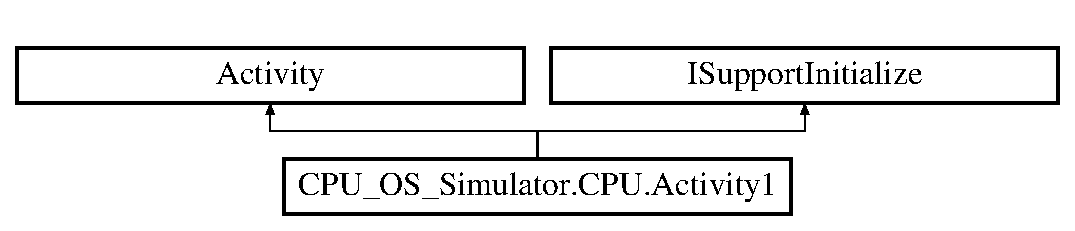
\includegraphics[height=2.000000cm]{class_c_p_u___o_s___simulator_1_1_c_p_u_1_1_activity1}
\end{center}
\end{figure}
\subsection*{Public Member Functions}
\begin{DoxyCompactItemize}
\item 
\hyperlink{class_c_p_u___o_s___simulator_1_1_c_p_u_1_1_activity1_afb3ce8aeef1cfe7c4a479f43327d5ea1}{Activity1} ()
\item 
void \hyperlink{class_c_p_u___o_s___simulator_1_1_c_p_u_1_1_activity1_a1a8dbcc92b48b1ca04bb667e96a89b10}{Initialize\+Component} ()
\begin{DoxyCompactList}\small\item\em Initialize\+Component \end{DoxyCompactList}\end{DoxyCompactItemize}
\subsection*{Private Member Functions}
\begin{DoxyCompactItemize}
\item 
partial void \hyperlink{class_c_p_u___o_s___simulator_1_1_c_p_u_1_1_activity1_a40e21e1735bdef0af255ee9f07fcb3d8}{Before\+Initialize\+Component} (ref bool is\+Initialized)
\item 
partial void \hyperlink{class_c_p_u___o_s___simulator_1_1_c_p_u_1_1_activity1_af4be750af1e09a820a79d78faf6caf4f}{After\+Initialize\+Component} ()
\item 
string \hyperlink{class_c_p_u___o_s___simulator_1_1_c_p_u_1_1_activity1_a841192007ebd277cd3e86f47e8d9c04b}{Find\+Resource} ()
\item 
void System.\+Component\+Model.\+I\+Support\+Initialize. \hyperlink{class_c_p_u___o_s___simulator_1_1_c_p_u_1_1_activity1_ae02f7230ddf93bd55c74ad47d9dc72e5}{Begin\+Init} ()
\item 
void System.\+Component\+Model.\+I\+Support\+Initialize. \hyperlink{class_c_p_u___o_s___simulator_1_1_c_p_u_1_1_activity1_a7d9c8128517a9b4a1a8860b3cc8ffd43}{End\+Init} ()
\end{DoxyCompactItemize}
\subsection*{Private Attributes}
\begin{DoxyCompactItemize}
\item 
bool \hyperlink{class_c_p_u___o_s___simulator_1_1_c_p_u_1_1_activity1_ae108a6148273acee3cfabe014d933386}{\+\_\+content\+Loaded}
\end{DoxyCompactItemize}


\subsection{Detailed Description}


Definition at line 16 of file Activity1.\+g.\+cs.



\subsection{Constructor \& Destructor Documentation}
\hypertarget{class_c_p_u___o_s___simulator_1_1_c_p_u_1_1_activity1_afb3ce8aeef1cfe7c4a479f43327d5ea1}{}\index{C\+P\+U\+\_\+\+O\+S\+\_\+\+Simulator\+::\+C\+P\+U\+::\+Activity1@{C\+P\+U\+\_\+\+O\+S\+\_\+\+Simulator\+::\+C\+P\+U\+::\+Activity1}!Activity1@{Activity1}}
\index{Activity1@{Activity1}!C\+P\+U\+\_\+\+O\+S\+\_\+\+Simulator\+::\+C\+P\+U\+::\+Activity1@{C\+P\+U\+\_\+\+O\+S\+\_\+\+Simulator\+::\+C\+P\+U\+::\+Activity1}}
\subsubsection[{Activity1()}]{\setlength{\rightskip}{0pt plus 5cm}C\+P\+U\+\_\+\+O\+S\+\_\+\+Simulator.\+C\+P\+U.\+Activity1.\+Activity1 (
\begin{DoxyParamCaption}
{}
\end{DoxyParamCaption}
)}\label{class_c_p_u___o_s___simulator_1_1_c_p_u_1_1_activity1_afb3ce8aeef1cfe7c4a479f43327d5ea1}


Definition at line 26 of file Activity1.\+g.\+cs.



\subsection{Member Function Documentation}
\hypertarget{class_c_p_u___o_s___simulator_1_1_c_p_u_1_1_activity1_af4be750af1e09a820a79d78faf6caf4f}{}\index{C\+P\+U\+\_\+\+O\+S\+\_\+\+Simulator\+::\+C\+P\+U\+::\+Activity1@{C\+P\+U\+\_\+\+O\+S\+\_\+\+Simulator\+::\+C\+P\+U\+::\+Activity1}!After\+Initialize\+Component@{After\+Initialize\+Component}}
\index{After\+Initialize\+Component@{After\+Initialize\+Component}!C\+P\+U\+\_\+\+O\+S\+\_\+\+Simulator\+::\+C\+P\+U\+::\+Activity1@{C\+P\+U\+\_\+\+O\+S\+\_\+\+Simulator\+::\+C\+P\+U\+::\+Activity1}}
\subsubsection[{After\+Initialize\+Component()}]{\setlength{\rightskip}{0pt plus 5cm}partial void C\+P\+U\+\_\+\+O\+S\+\_\+\+Simulator.\+C\+P\+U.\+Activity1.\+After\+Initialize\+Component (
\begin{DoxyParamCaption}
{}
\end{DoxyParamCaption}
)\hspace{0.3cm}{\ttfamily [private]}}\label{class_c_p_u___o_s___simulator_1_1_c_p_u_1_1_activity1_af4be750af1e09a820a79d78faf6caf4f}
\hypertarget{class_c_p_u___o_s___simulator_1_1_c_p_u_1_1_activity1_a40e21e1735bdef0af255ee9f07fcb3d8}{}\index{C\+P\+U\+\_\+\+O\+S\+\_\+\+Simulator\+::\+C\+P\+U\+::\+Activity1@{C\+P\+U\+\_\+\+O\+S\+\_\+\+Simulator\+::\+C\+P\+U\+::\+Activity1}!Before\+Initialize\+Component@{Before\+Initialize\+Component}}
\index{Before\+Initialize\+Component@{Before\+Initialize\+Component}!C\+P\+U\+\_\+\+O\+S\+\_\+\+Simulator\+::\+C\+P\+U\+::\+Activity1@{C\+P\+U\+\_\+\+O\+S\+\_\+\+Simulator\+::\+C\+P\+U\+::\+Activity1}}
\subsubsection[{Before\+Initialize\+Component(ref bool is\+Initialized)}]{\setlength{\rightskip}{0pt plus 5cm}partial void C\+P\+U\+\_\+\+O\+S\+\_\+\+Simulator.\+C\+P\+U.\+Activity1.\+Before\+Initialize\+Component (
\begin{DoxyParamCaption}
\item[{ref bool}]{is\+Initialized}
\end{DoxyParamCaption}
)\hspace{0.3cm}{\ttfamily [private]}}\label{class_c_p_u___o_s___simulator_1_1_c_p_u_1_1_activity1_a40e21e1735bdef0af255ee9f07fcb3d8}
\hypertarget{class_c_p_u___o_s___simulator_1_1_c_p_u_1_1_activity1_ae02f7230ddf93bd55c74ad47d9dc72e5}{}\index{C\+P\+U\+\_\+\+O\+S\+\_\+\+Simulator\+::\+C\+P\+U\+::\+Activity1@{C\+P\+U\+\_\+\+O\+S\+\_\+\+Simulator\+::\+C\+P\+U\+::\+Activity1}!Begin\+Init@{Begin\+Init}}
\index{Begin\+Init@{Begin\+Init}!C\+P\+U\+\_\+\+O\+S\+\_\+\+Simulator\+::\+C\+P\+U\+::\+Activity1@{C\+P\+U\+\_\+\+O\+S\+\_\+\+Simulator\+::\+C\+P\+U\+::\+Activity1}}
\subsubsection[{Begin\+Init()}]{\setlength{\rightskip}{0pt plus 5cm}void System.\+Component\+Model.\+I\+Support\+Initialize. C\+P\+U\+\_\+\+O\+S\+\_\+\+Simulator.\+C\+P\+U.\+Activity1.\+Begin\+Init (
\begin{DoxyParamCaption}
{}
\end{DoxyParamCaption}
)\hspace{0.3cm}{\ttfamily [private]}}\label{class_c_p_u___o_s___simulator_1_1_c_p_u_1_1_activity1_ae02f7230ddf93bd55c74ad47d9dc72e5}


Definition at line 92 of file Activity1.\+g.\+cs.

\hypertarget{class_c_p_u___o_s___simulator_1_1_c_p_u_1_1_activity1_a7d9c8128517a9b4a1a8860b3cc8ffd43}{}\index{C\+P\+U\+\_\+\+O\+S\+\_\+\+Simulator\+::\+C\+P\+U\+::\+Activity1@{C\+P\+U\+\_\+\+O\+S\+\_\+\+Simulator\+::\+C\+P\+U\+::\+Activity1}!End\+Init@{End\+Init}}
\index{End\+Init@{End\+Init}!C\+P\+U\+\_\+\+O\+S\+\_\+\+Simulator\+::\+C\+P\+U\+::\+Activity1@{C\+P\+U\+\_\+\+O\+S\+\_\+\+Simulator\+::\+C\+P\+U\+::\+Activity1}}
\subsubsection[{End\+Init()}]{\setlength{\rightskip}{0pt plus 5cm}void System.\+Component\+Model.\+I\+Support\+Initialize. C\+P\+U\+\_\+\+O\+S\+\_\+\+Simulator.\+C\+P\+U.\+Activity1.\+End\+Init (
\begin{DoxyParamCaption}
{}
\end{DoxyParamCaption}
)\hspace{0.3cm}{\ttfamily [private]}}\label{class_c_p_u___o_s___simulator_1_1_c_p_u_1_1_activity1_a7d9c8128517a9b4a1a8860b3cc8ffd43}


Definition at line 97 of file Activity1.\+g.\+cs.

\hypertarget{class_c_p_u___o_s___simulator_1_1_c_p_u_1_1_activity1_a841192007ebd277cd3e86f47e8d9c04b}{}\index{C\+P\+U\+\_\+\+O\+S\+\_\+\+Simulator\+::\+C\+P\+U\+::\+Activity1@{C\+P\+U\+\_\+\+O\+S\+\_\+\+Simulator\+::\+C\+P\+U\+::\+Activity1}!Find\+Resource@{Find\+Resource}}
\index{Find\+Resource@{Find\+Resource}!C\+P\+U\+\_\+\+O\+S\+\_\+\+Simulator\+::\+C\+P\+U\+::\+Activity1@{C\+P\+U\+\_\+\+O\+S\+\_\+\+Simulator\+::\+C\+P\+U\+::\+Activity1}}
\subsubsection[{Find\+Resource()}]{\setlength{\rightskip}{0pt plus 5cm}string C\+P\+U\+\_\+\+O\+S\+\_\+\+Simulator.\+C\+P\+U.\+Activity1.\+Find\+Resource (
\begin{DoxyParamCaption}
{}
\end{DoxyParamCaption}
)\hspace{0.3cm}{\ttfamily [private]}}\label{class_c_p_u___o_s___simulator_1_1_c_p_u_1_1_activity1_a841192007ebd277cd3e86f47e8d9c04b}


Definition at line 79 of file Activity1.\+g.\+cs.

\hypertarget{class_c_p_u___o_s___simulator_1_1_c_p_u_1_1_activity1_a1a8dbcc92b48b1ca04bb667e96a89b10}{}\index{C\+P\+U\+\_\+\+O\+S\+\_\+\+Simulator\+::\+C\+P\+U\+::\+Activity1@{C\+P\+U\+\_\+\+O\+S\+\_\+\+Simulator\+::\+C\+P\+U\+::\+Activity1}!Initialize\+Component@{Initialize\+Component}}
\index{Initialize\+Component@{Initialize\+Component}!C\+P\+U\+\_\+\+O\+S\+\_\+\+Simulator\+::\+C\+P\+U\+::\+Activity1@{C\+P\+U\+\_\+\+O\+S\+\_\+\+Simulator\+::\+C\+P\+U\+::\+Activity1}}
\subsubsection[{Initialize\+Component()}]{\setlength{\rightskip}{0pt plus 5cm}void C\+P\+U\+\_\+\+O\+S\+\_\+\+Simulator.\+C\+P\+U.\+Activity1.\+Initialize\+Component (
\begin{DoxyParamCaption}
{}
\end{DoxyParamCaption}
)}\label{class_c_p_u___o_s___simulator_1_1_c_p_u_1_1_activity1_a1a8dbcc92b48b1ca04bb667e96a89b10}


Initialize\+Component 



Definition at line 35 of file Activity1.\+g.\+cs.



\subsection{Member Data Documentation}
\hypertarget{class_c_p_u___o_s___simulator_1_1_c_p_u_1_1_activity1_ae108a6148273acee3cfabe014d933386}{}\index{C\+P\+U\+\_\+\+O\+S\+\_\+\+Simulator\+::\+C\+P\+U\+::\+Activity1@{C\+P\+U\+\_\+\+O\+S\+\_\+\+Simulator\+::\+C\+P\+U\+::\+Activity1}!\+\_\+content\+Loaded@{\+\_\+content\+Loaded}}
\index{\+\_\+content\+Loaded@{\+\_\+content\+Loaded}!C\+P\+U\+\_\+\+O\+S\+\_\+\+Simulator\+::\+C\+P\+U\+::\+Activity1@{C\+P\+U\+\_\+\+O\+S\+\_\+\+Simulator\+::\+C\+P\+U\+::\+Activity1}}
\subsubsection[{\+\_\+content\+Loaded}]{\setlength{\rightskip}{0pt plus 5cm}bool C\+P\+U\+\_\+\+O\+S\+\_\+\+Simulator.\+C\+P\+U.\+Activity1.\+\_\+content\+Loaded\hspace{0.3cm}{\ttfamily [private]}}\label{class_c_p_u___o_s___simulator_1_1_c_p_u_1_1_activity1_ae108a6148273acee3cfabe014d933386}


Definition at line 18 of file Activity1.\+g.\+cs.



The documentation for this class was generated from the following file\+:\begin{DoxyCompactItemize}
\item 
C\+P\+U/obj/\+Debug/\+In\+Process\+Temp\+Files/\hyperlink{_activity1_8g_8cs}{Activity1.\+g.\+cs}\end{DoxyCompactItemize}

\hypertarget{class_c_p_u___o_s___simulator_1_1_app}{}\section{C\+P\+U\+\_\+\+O\+S\+\_\+\+Simulator.\+App Class Reference}
\label{class_c_p_u___o_s___simulator_1_1_app}\index{C\+P\+U\+\_\+\+O\+S\+\_\+\+Simulator.\+App@{C\+P\+U\+\_\+\+O\+S\+\_\+\+Simulator.\+App}}


Interaction logic for App.\+xaml  


Inheritance diagram for C\+P\+U\+\_\+\+O\+S\+\_\+\+Simulator.\+App\+:\begin{figure}[H]
\begin{center}
\leavevmode
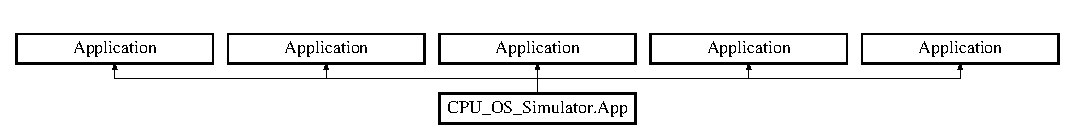
\includegraphics[height=2.000000cm]{class_c_p_u___o_s___simulator_1_1_app}
\end{center}
\end{figure}
\subsection*{Public Member Functions}
\begin{DoxyCompactItemize}
\item 
void \hyperlink{class_c_p_u___o_s___simulator_1_1_app_a15e2e0e02c8dbe7d5d3fba5d21f3e56f}{Initialize\+Component} ()
\begin{DoxyCompactList}\small\item\em Initialize\+Component \end{DoxyCompactList}\item 
void \hyperlink{class_c_p_u___o_s___simulator_1_1_app_a15e2e0e02c8dbe7d5d3fba5d21f3e56f}{Initialize\+Component} ()
\begin{DoxyCompactList}\small\item\em Initialize\+Component \end{DoxyCompactList}\end{DoxyCompactItemize}
\subsection*{Static Public Member Functions}
\begin{DoxyCompactItemize}
\item 
static void \hyperlink{class_c_p_u___o_s___simulator_1_1_app_a7bbb69f458b77923e336283b1653ce69}{Main} ()
\begin{DoxyCompactList}\small\item\em Application Entry Point. \end{DoxyCompactList}\item 
static void \hyperlink{class_c_p_u___o_s___simulator_1_1_app_a7bbb69f458b77923e336283b1653ce69}{Main} ()
\begin{DoxyCompactList}\small\item\em Application Entry Point. \end{DoxyCompactList}\end{DoxyCompactItemize}


\subsection{Detailed Description}
Interaction logic for App.\+xaml 

\hyperlink{class_c_p_u___o_s___simulator_1_1_app}{App} 

Definition at line 8 of file App.\+xaml.\+cs.



\subsection{Member Function Documentation}
\hypertarget{class_c_p_u___o_s___simulator_1_1_app_a15e2e0e02c8dbe7d5d3fba5d21f3e56f}{}\index{C\+P\+U\+\_\+\+O\+S\+\_\+\+Simulator\+::\+App@{C\+P\+U\+\_\+\+O\+S\+\_\+\+Simulator\+::\+App}!Initialize\+Component@{Initialize\+Component}}
\index{Initialize\+Component@{Initialize\+Component}!C\+P\+U\+\_\+\+O\+S\+\_\+\+Simulator\+::\+App@{C\+P\+U\+\_\+\+O\+S\+\_\+\+Simulator\+::\+App}}
\subsubsection[{Initialize\+Component()}]{\setlength{\rightskip}{0pt plus 5cm}void C\+P\+U\+\_\+\+O\+S\+\_\+\+Simulator.\+App.\+Initialize\+Component (
\begin{DoxyParamCaption}
{}
\end{DoxyParamCaption}
)}\label{class_c_p_u___o_s___simulator_1_1_app_a15e2e0e02c8dbe7d5d3fba5d21f3e56f}


Initialize\+Component 



Definition at line 48 of file App.\+g.\+cs.

\hypertarget{class_c_p_u___o_s___simulator_1_1_app_a15e2e0e02c8dbe7d5d3fba5d21f3e56f}{}\index{C\+P\+U\+\_\+\+O\+S\+\_\+\+Simulator\+::\+App@{C\+P\+U\+\_\+\+O\+S\+\_\+\+Simulator\+::\+App}!Initialize\+Component@{Initialize\+Component}}
\index{Initialize\+Component@{Initialize\+Component}!C\+P\+U\+\_\+\+O\+S\+\_\+\+Simulator\+::\+App@{C\+P\+U\+\_\+\+O\+S\+\_\+\+Simulator\+::\+App}}
\subsubsection[{Initialize\+Component()}]{\setlength{\rightskip}{0pt plus 5cm}void C\+P\+U\+\_\+\+O\+S\+\_\+\+Simulator.\+App.\+Initialize\+Component (
\begin{DoxyParamCaption}
{}
\end{DoxyParamCaption}
)}\label{class_c_p_u___o_s___simulator_1_1_app_a15e2e0e02c8dbe7d5d3fba5d21f3e56f}


Initialize\+Component 



Definition at line 48 of file App.\+g.\+i.\+cs.

\hypertarget{class_c_p_u___o_s___simulator_1_1_app_a7bbb69f458b77923e336283b1653ce69}{}\index{C\+P\+U\+\_\+\+O\+S\+\_\+\+Simulator\+::\+App@{C\+P\+U\+\_\+\+O\+S\+\_\+\+Simulator\+::\+App}!Main@{Main}}
\index{Main@{Main}!C\+P\+U\+\_\+\+O\+S\+\_\+\+Simulator\+::\+App@{C\+P\+U\+\_\+\+O\+S\+\_\+\+Simulator\+::\+App}}
\subsubsection[{Main()}]{\setlength{\rightskip}{0pt plus 5cm}static void C\+P\+U\+\_\+\+O\+S\+\_\+\+Simulator.\+App.\+Main (
\begin{DoxyParamCaption}
{}
\end{DoxyParamCaption}
)\hspace{0.3cm}{\ttfamily [static]}}\label{class_c_p_u___o_s___simulator_1_1_app_a7bbb69f458b77923e336283b1653ce69}


Application Entry Point. 



Definition at line 63 of file App.\+g.\+i.\+cs.

\hypertarget{class_c_p_u___o_s___simulator_1_1_app_a7bbb69f458b77923e336283b1653ce69}{}\index{C\+P\+U\+\_\+\+O\+S\+\_\+\+Simulator\+::\+App@{C\+P\+U\+\_\+\+O\+S\+\_\+\+Simulator\+::\+App}!Main@{Main}}
\index{Main@{Main}!C\+P\+U\+\_\+\+O\+S\+\_\+\+Simulator\+::\+App@{C\+P\+U\+\_\+\+O\+S\+\_\+\+Simulator\+::\+App}}
\subsubsection[{Main()}]{\setlength{\rightskip}{0pt plus 5cm}static void C\+P\+U\+\_\+\+O\+S\+\_\+\+Simulator.\+App.\+Main (
\begin{DoxyParamCaption}
{}
\end{DoxyParamCaption}
)\hspace{0.3cm}{\ttfamily [static]}}\label{class_c_p_u___o_s___simulator_1_1_app_a7bbb69f458b77923e336283b1653ce69}


Application Entry Point. 



Definition at line 63 of file App.\+g.\+cs.



The documentation for this class was generated from the following files\+:\begin{DoxyCompactItemize}
\item 
C\+P\+U-\/\+O\+S Simulator/\hyperlink{_app_8xaml_8cs}{App.\+xaml.\+cs}\item 
C\+P\+U-\/\+O\+S Simulator/obj/\+Debug/\hyperlink{_app_8g_8cs}{App.\+g.\+cs}\item 
C\+P\+U-\/\+O\+S Simulator/obj/\+Debug/\hyperlink{_app_8g_8i_8cs}{App.\+g.\+i.\+cs}\end{DoxyCompactItemize}

\hypertarget{class_c_p_u___o_s___simulator_1_1_c_p_u_1_1_execution_unit}{}\section{C\+P\+U\+\_\+\+O\+S\+\_\+\+Simulator.\+C\+P\+U.\+Execution\+Unit Class Reference}
\label{class_c_p_u___o_s___simulator_1_1_c_p_u_1_1_execution_unit}\index{C\+P\+U\+\_\+\+O\+S\+\_\+\+Simulator.\+C\+P\+U.\+Execution\+Unit@{C\+P\+U\+\_\+\+O\+S\+\_\+\+Simulator.\+C\+P\+U.\+Execution\+Unit}}


This class represents the part of the \hyperlink{namespace_c_p_u___o_s___simulator_1_1_c_p_u}{C\+P\+U} which executes instructions  


\subsection*{Public Member Functions}
\begin{DoxyCompactItemize}
\item 
\hyperlink{class_c_p_u___o_s___simulator_1_1_c_p_u_1_1_execution_unit_aaa72bccee27d810d5bbfa9ed02215fa9}{Execution\+Unit} (\hyperlink{class_c_p_u___o_s___simulator_1_1_c_p_u_1_1_simulator_program}{Simulator\+Program} \hyperlink{class_c_p_u___o_s___simulator_1_1_c_p_u_1_1_execution_unit_a192670bee8ca089c38e9989350f658d6}{program}, int \hyperlink{class_c_p_u___o_s___simulator_1_1_c_p_u_1_1_execution_unit_a0deb0a3e0c9fa402598bbf18be6535cc}{clock\+Speed})
\begin{DoxyCompactList}\small\item\em Constructor for execution unit that starts executing from the beginning of the program \end{DoxyCompactList}\item 
\hyperlink{class_c_p_u___o_s___simulator_1_1_c_p_u_1_1_execution_unit_a0b69abfef40692e266fee90b2321797e}{Execution\+Unit} (\hyperlink{class_c_p_u___o_s___simulator_1_1_c_p_u_1_1_simulator_program}{Simulator\+Program} \hyperlink{class_c_p_u___o_s___simulator_1_1_c_p_u_1_1_execution_unit_a192670bee8ca089c38e9989350f658d6}{program}, int \hyperlink{class_c_p_u___o_s___simulator_1_1_c_p_u_1_1_execution_unit_a0deb0a3e0c9fa402598bbf18be6535cc}{clock\+Speed}, int \hyperlink{class_c_p_u___o_s___simulator_1_1_c_p_u_1_1_execution_unit_af6807cb5343acc2c40a08166c748f1f0}{current\+Index})
\begin{DoxyCompactList}\small\item\em Constructor for execution unit that starts executing from a specified location in the program \end{DoxyCompactList}\item 
void \hyperlink{class_c_p_u___o_s___simulator_1_1_c_p_u_1_1_execution_unit_ae0298423e5e7aad47e342e3960a361ac}{Execute\+Instruction} ()
\begin{DoxyCompactList}\small\item\em This function executes an instruction by calling its delegate function \end{DoxyCompactList}\end{DoxyCompactItemize}
\subsection*{Properties}
\begin{DoxyCompactItemize}
\item 
\hyperlink{class_c_p_u___o_s___simulator_1_1_c_p_u_1_1_simulator_program}{Simulator\+Program} \hyperlink{class_c_p_u___o_s___simulator_1_1_c_p_u_1_1_execution_unit_a5266ac137491de1efa6c4d707fcd162e}{Program}\hspace{0.3cm}{\ttfamily  \mbox{[}get, set\mbox{]}}
\item 
int \hyperlink{class_c_p_u___o_s___simulator_1_1_c_p_u_1_1_execution_unit_ac34a0c232ee8d1996d29f5d8614556ab}{Clock\+Speed}\hspace{0.3cm}{\ttfamily  \mbox{[}get, set\mbox{]}}
\item 
bool \hyperlink{class_c_p_u___o_s___simulator_1_1_c_p_u_1_1_execution_unit_a1b8748f1c6679263e5dc03fe382ad150}{Stop}\hspace{0.3cm}{\ttfamily  \mbox{[}get, set\mbox{]}}
\item 
bool \hyperlink{class_c_p_u___o_s___simulator_1_1_c_p_u_1_1_execution_unit_afc47977290c9bccf4f3b115613a67576}{Done}\hspace{0.3cm}{\ttfamily  \mbox{[}get, set\mbox{]}}
\item 
int \hyperlink{class_c_p_u___o_s___simulator_1_1_c_p_u_1_1_execution_unit_a14d2a23bdc679ed2758733f34f79db63}{Current\+Index}\hspace{0.3cm}{\ttfamily  \mbox{[}get, set\mbox{]}}
\item 
int \hyperlink{class_c_p_u___o_s___simulator_1_1_c_p_u_1_1_execution_unit_ac939e9a08b30b2cc3a9438d6c1cc5a61}{Logical\+Address}\hspace{0.3cm}{\ttfamily  \mbox{[}get, set\mbox{]}}
\item 
\hyperlink{class_c_p_u___o_s___simulator_1_1_c_p_u_1_1_instruction}{Instruction} \hyperlink{class_c_p_u___o_s___simulator_1_1_c_p_u_1_1_execution_unit_a285d7b487a3ac5eff07c640e438ceb11}{Current\+Instruction}\hspace{0.3cm}{\ttfamily  \mbox{[}get, set\mbox{]}}
\end{DoxyCompactItemize}
\subsection*{Private Attributes}
\begin{DoxyCompactItemize}
\item 
\hyperlink{class_c_p_u___o_s___simulator_1_1_c_p_u_1_1_simulator_program}{Simulator\+Program} \hyperlink{class_c_p_u___o_s___simulator_1_1_c_p_u_1_1_execution_unit_a192670bee8ca089c38e9989350f658d6}{program}
\begin{DoxyCompactList}\small\item\em The current program being executed \end{DoxyCompactList}\item 
int \hyperlink{class_c_p_u___o_s___simulator_1_1_c_p_u_1_1_execution_unit_a0deb0a3e0c9fa402598bbf18be6535cc}{clock\+Speed}
\begin{DoxyCompactList}\small\item\em The clock speed that the \hyperlink{namespace_c_p_u___o_s___simulator_1_1_c_p_u}{C\+P\+U} is running at \end{DoxyCompactList}\item 
int \hyperlink{class_c_p_u___o_s___simulator_1_1_c_p_u_1_1_execution_unit_af6807cb5343acc2c40a08166c748f1f0}{current\+Index}
\begin{DoxyCompactList}\small\item\em The index of the instruction currently being executed \end{DoxyCompactList}\item 
\hyperlink{class_c_p_u___o_s___simulator_1_1_c_p_u_1_1_instruction}{Instruction} \hyperlink{class_c_p_u___o_s___simulator_1_1_c_p_u_1_1_execution_unit_a12fc8d1fd19eab177941b9f98675eb7f}{current\+Instruction}
\begin{DoxyCompactList}\small\item\em The instruction currently being executed \end{DoxyCompactList}\item 
int \hyperlink{class_c_p_u___o_s___simulator_1_1_c_p_u_1_1_execution_unit_aa387f2bbbf0de1c75cbd1c79e27a630c}{logical\+Address}
\begin{DoxyCompactList}\small\item\em The Logical address of the instruction currently being executed \end{DoxyCompactList}\item 
bool \hyperlink{class_c_p_u___o_s___simulator_1_1_c_p_u_1_1_execution_unit_aad508435c1085ec880b75723260b0439}{stop}
\begin{DoxyCompactList}\small\item\em Whether the unit has received a stop signal from the main window \end{DoxyCompactList}\item 
bool \hyperlink{class_c_p_u___o_s___simulator_1_1_c_p_u_1_1_execution_unit_aa62cb66691fd4d782a4fa5c70843da6e}{done}
\begin{DoxyCompactList}\small\item\em Whether the unit has reached the end of the program \end{DoxyCompactList}\end{DoxyCompactItemize}


\subsection{Detailed Description}
This class represents the part of the \hyperlink{namespace_c_p_u___o_s___simulator_1_1_c_p_u}{C\+P\+U} which executes instructions 



Definition at line 10 of file Execution\+Unit.\+cs.



\subsection{Constructor \& Destructor Documentation}
\hypertarget{class_c_p_u___o_s___simulator_1_1_c_p_u_1_1_execution_unit_aaa72bccee27d810d5bbfa9ed02215fa9}{}\index{C\+P\+U\+\_\+\+O\+S\+\_\+\+Simulator\+::\+C\+P\+U\+::\+Execution\+Unit@{C\+P\+U\+\_\+\+O\+S\+\_\+\+Simulator\+::\+C\+P\+U\+::\+Execution\+Unit}!Execution\+Unit@{Execution\+Unit}}
\index{Execution\+Unit@{Execution\+Unit}!C\+P\+U\+\_\+\+O\+S\+\_\+\+Simulator\+::\+C\+P\+U\+::\+Execution\+Unit@{C\+P\+U\+\_\+\+O\+S\+\_\+\+Simulator\+::\+C\+P\+U\+::\+Execution\+Unit}}
\subsubsection[{Execution\+Unit(\+Simulator\+Program program, int clock\+Speed)}]{\setlength{\rightskip}{0pt plus 5cm}C\+P\+U\+\_\+\+O\+S\+\_\+\+Simulator.\+C\+P\+U.\+Execution\+Unit.\+Execution\+Unit (
\begin{DoxyParamCaption}
\item[{{\bf Simulator\+Program}}]{program, }
\item[{int}]{clock\+Speed}
\end{DoxyParamCaption}
)}\label{class_c_p_u___o_s___simulator_1_1_c_p_u_1_1_execution_unit_aaa72bccee27d810d5bbfa9ed02215fa9}


Constructor for execution unit that starts executing from the beginning of the program 


\begin{DoxyParams}{Parameters}
{\em program} & the program to execute \\
\hline
{\em clock\+Speed} & the clock speed of the \hyperlink{namespace_c_p_u___o_s___simulator_1_1_c_p_u}{C\+P\+U} \\
\hline
\end{DoxyParams}


Definition at line 58 of file Execution\+Unit.\+cs.

\hypertarget{class_c_p_u___o_s___simulator_1_1_c_p_u_1_1_execution_unit_a0b69abfef40692e266fee90b2321797e}{}\index{C\+P\+U\+\_\+\+O\+S\+\_\+\+Simulator\+::\+C\+P\+U\+::\+Execution\+Unit@{C\+P\+U\+\_\+\+O\+S\+\_\+\+Simulator\+::\+C\+P\+U\+::\+Execution\+Unit}!Execution\+Unit@{Execution\+Unit}}
\index{Execution\+Unit@{Execution\+Unit}!C\+P\+U\+\_\+\+O\+S\+\_\+\+Simulator\+::\+C\+P\+U\+::\+Execution\+Unit@{C\+P\+U\+\_\+\+O\+S\+\_\+\+Simulator\+::\+C\+P\+U\+::\+Execution\+Unit}}
\subsubsection[{Execution\+Unit(\+Simulator\+Program program, int clock\+Speed, int current\+Index)}]{\setlength{\rightskip}{0pt plus 5cm}C\+P\+U\+\_\+\+O\+S\+\_\+\+Simulator.\+C\+P\+U.\+Execution\+Unit.\+Execution\+Unit (
\begin{DoxyParamCaption}
\item[{{\bf Simulator\+Program}}]{program, }
\item[{int}]{clock\+Speed, }
\item[{int}]{current\+Index}
\end{DoxyParamCaption}
)}\label{class_c_p_u___o_s___simulator_1_1_c_p_u_1_1_execution_unit_a0b69abfef40692e266fee90b2321797e}


Constructor for execution unit that starts executing from a specified location in the program 


\begin{DoxyParams}{Parameters}
{\em program} & the program to execute \\
\hline
{\em current\+Index} & the index to start executing from\\
\hline
{\em clock\+Speed} & the clock speed of the \hyperlink{namespace_c_p_u___o_s___simulator_1_1_c_p_u}{C\+P\+U} \\
\hline
\end{DoxyParams}


Definition at line 75 of file Execution\+Unit.\+cs.



\subsection{Member Function Documentation}
\hypertarget{class_c_p_u___o_s___simulator_1_1_c_p_u_1_1_execution_unit_ae0298423e5e7aad47e342e3960a361ac}{}\index{C\+P\+U\+\_\+\+O\+S\+\_\+\+Simulator\+::\+C\+P\+U\+::\+Execution\+Unit@{C\+P\+U\+\_\+\+O\+S\+\_\+\+Simulator\+::\+C\+P\+U\+::\+Execution\+Unit}!Execute\+Instruction@{Execute\+Instruction}}
\index{Execute\+Instruction@{Execute\+Instruction}!C\+P\+U\+\_\+\+O\+S\+\_\+\+Simulator\+::\+C\+P\+U\+::\+Execution\+Unit@{C\+P\+U\+\_\+\+O\+S\+\_\+\+Simulator\+::\+C\+P\+U\+::\+Execution\+Unit}}
\subsubsection[{Execute\+Instruction()}]{\setlength{\rightskip}{0pt plus 5cm}void C\+P\+U\+\_\+\+O\+S\+\_\+\+Simulator.\+C\+P\+U.\+Execution\+Unit.\+Execute\+Instruction (
\begin{DoxyParamCaption}
{}
\end{DoxyParamCaption}
)}\label{class_c_p_u___o_s___simulator_1_1_c_p_u_1_1_execution_unit_ae0298423e5e7aad47e342e3960a361ac}


This function executes an instruction by calling its delegate function 



Definition at line 95 of file Execution\+Unit.\+cs.



\subsection{Member Data Documentation}
\hypertarget{class_c_p_u___o_s___simulator_1_1_c_p_u_1_1_execution_unit_a0deb0a3e0c9fa402598bbf18be6535cc}{}\index{C\+P\+U\+\_\+\+O\+S\+\_\+\+Simulator\+::\+C\+P\+U\+::\+Execution\+Unit@{C\+P\+U\+\_\+\+O\+S\+\_\+\+Simulator\+::\+C\+P\+U\+::\+Execution\+Unit}!clock\+Speed@{clock\+Speed}}
\index{clock\+Speed@{clock\+Speed}!C\+P\+U\+\_\+\+O\+S\+\_\+\+Simulator\+::\+C\+P\+U\+::\+Execution\+Unit@{C\+P\+U\+\_\+\+O\+S\+\_\+\+Simulator\+::\+C\+P\+U\+::\+Execution\+Unit}}
\subsubsection[{clock\+Speed}]{\setlength{\rightskip}{0pt plus 5cm}int C\+P\+U\+\_\+\+O\+S\+\_\+\+Simulator.\+C\+P\+U.\+Execution\+Unit.\+clock\+Speed\hspace{0.3cm}{\ttfamily [private]}}\label{class_c_p_u___o_s___simulator_1_1_c_p_u_1_1_execution_unit_a0deb0a3e0c9fa402598bbf18be6535cc}


The clock speed that the \hyperlink{namespace_c_p_u___o_s___simulator_1_1_c_p_u}{C\+P\+U} is running at 



Definition at line 22 of file Execution\+Unit.\+cs.

\hypertarget{class_c_p_u___o_s___simulator_1_1_c_p_u_1_1_execution_unit_af6807cb5343acc2c40a08166c748f1f0}{}\index{C\+P\+U\+\_\+\+O\+S\+\_\+\+Simulator\+::\+C\+P\+U\+::\+Execution\+Unit@{C\+P\+U\+\_\+\+O\+S\+\_\+\+Simulator\+::\+C\+P\+U\+::\+Execution\+Unit}!current\+Index@{current\+Index}}
\index{current\+Index@{current\+Index}!C\+P\+U\+\_\+\+O\+S\+\_\+\+Simulator\+::\+C\+P\+U\+::\+Execution\+Unit@{C\+P\+U\+\_\+\+O\+S\+\_\+\+Simulator\+::\+C\+P\+U\+::\+Execution\+Unit}}
\subsubsection[{current\+Index}]{\setlength{\rightskip}{0pt plus 5cm}int C\+P\+U\+\_\+\+O\+S\+\_\+\+Simulator.\+C\+P\+U.\+Execution\+Unit.\+current\+Index\hspace{0.3cm}{\ttfamily [private]}}\label{class_c_p_u___o_s___simulator_1_1_c_p_u_1_1_execution_unit_af6807cb5343acc2c40a08166c748f1f0}


The index of the instruction currently being executed 



Definition at line 27 of file Execution\+Unit.\+cs.

\hypertarget{class_c_p_u___o_s___simulator_1_1_c_p_u_1_1_execution_unit_a12fc8d1fd19eab177941b9f98675eb7f}{}\index{C\+P\+U\+\_\+\+O\+S\+\_\+\+Simulator\+::\+C\+P\+U\+::\+Execution\+Unit@{C\+P\+U\+\_\+\+O\+S\+\_\+\+Simulator\+::\+C\+P\+U\+::\+Execution\+Unit}!current\+Instruction@{current\+Instruction}}
\index{current\+Instruction@{current\+Instruction}!C\+P\+U\+\_\+\+O\+S\+\_\+\+Simulator\+::\+C\+P\+U\+::\+Execution\+Unit@{C\+P\+U\+\_\+\+O\+S\+\_\+\+Simulator\+::\+C\+P\+U\+::\+Execution\+Unit}}
\subsubsection[{current\+Instruction}]{\setlength{\rightskip}{0pt plus 5cm}{\bf Instruction} C\+P\+U\+\_\+\+O\+S\+\_\+\+Simulator.\+C\+P\+U.\+Execution\+Unit.\+current\+Instruction\hspace{0.3cm}{\ttfamily [private]}}\label{class_c_p_u___o_s___simulator_1_1_c_p_u_1_1_execution_unit_a12fc8d1fd19eab177941b9f98675eb7f}


The instruction currently being executed 



Definition at line 32 of file Execution\+Unit.\+cs.

\hypertarget{class_c_p_u___o_s___simulator_1_1_c_p_u_1_1_execution_unit_aa62cb66691fd4d782a4fa5c70843da6e}{}\index{C\+P\+U\+\_\+\+O\+S\+\_\+\+Simulator\+::\+C\+P\+U\+::\+Execution\+Unit@{C\+P\+U\+\_\+\+O\+S\+\_\+\+Simulator\+::\+C\+P\+U\+::\+Execution\+Unit}!done@{done}}
\index{done@{done}!C\+P\+U\+\_\+\+O\+S\+\_\+\+Simulator\+::\+C\+P\+U\+::\+Execution\+Unit@{C\+P\+U\+\_\+\+O\+S\+\_\+\+Simulator\+::\+C\+P\+U\+::\+Execution\+Unit}}
\subsubsection[{done}]{\setlength{\rightskip}{0pt plus 5cm}bool C\+P\+U\+\_\+\+O\+S\+\_\+\+Simulator.\+C\+P\+U.\+Execution\+Unit.\+done\hspace{0.3cm}{\ttfamily [private]}}\label{class_c_p_u___o_s___simulator_1_1_c_p_u_1_1_execution_unit_aa62cb66691fd4d782a4fa5c70843da6e}


Whether the unit has reached the end of the program 



Definition at line 47 of file Execution\+Unit.\+cs.

\hypertarget{class_c_p_u___o_s___simulator_1_1_c_p_u_1_1_execution_unit_aa387f2bbbf0de1c75cbd1c79e27a630c}{}\index{C\+P\+U\+\_\+\+O\+S\+\_\+\+Simulator\+::\+C\+P\+U\+::\+Execution\+Unit@{C\+P\+U\+\_\+\+O\+S\+\_\+\+Simulator\+::\+C\+P\+U\+::\+Execution\+Unit}!logical\+Address@{logical\+Address}}
\index{logical\+Address@{logical\+Address}!C\+P\+U\+\_\+\+O\+S\+\_\+\+Simulator\+::\+C\+P\+U\+::\+Execution\+Unit@{C\+P\+U\+\_\+\+O\+S\+\_\+\+Simulator\+::\+C\+P\+U\+::\+Execution\+Unit}}
\subsubsection[{logical\+Address}]{\setlength{\rightskip}{0pt plus 5cm}int C\+P\+U\+\_\+\+O\+S\+\_\+\+Simulator.\+C\+P\+U.\+Execution\+Unit.\+logical\+Address\hspace{0.3cm}{\ttfamily [private]}}\label{class_c_p_u___o_s___simulator_1_1_c_p_u_1_1_execution_unit_aa387f2bbbf0de1c75cbd1c79e27a630c}


The Logical address of the instruction currently being executed 



Definition at line 37 of file Execution\+Unit.\+cs.

\hypertarget{class_c_p_u___o_s___simulator_1_1_c_p_u_1_1_execution_unit_a192670bee8ca089c38e9989350f658d6}{}\index{C\+P\+U\+\_\+\+O\+S\+\_\+\+Simulator\+::\+C\+P\+U\+::\+Execution\+Unit@{C\+P\+U\+\_\+\+O\+S\+\_\+\+Simulator\+::\+C\+P\+U\+::\+Execution\+Unit}!program@{program}}
\index{program@{program}!C\+P\+U\+\_\+\+O\+S\+\_\+\+Simulator\+::\+C\+P\+U\+::\+Execution\+Unit@{C\+P\+U\+\_\+\+O\+S\+\_\+\+Simulator\+::\+C\+P\+U\+::\+Execution\+Unit}}
\subsubsection[{program}]{\setlength{\rightskip}{0pt plus 5cm}{\bf Simulator\+Program} C\+P\+U\+\_\+\+O\+S\+\_\+\+Simulator.\+C\+P\+U.\+Execution\+Unit.\+program\hspace{0.3cm}{\ttfamily [private]}}\label{class_c_p_u___o_s___simulator_1_1_c_p_u_1_1_execution_unit_a192670bee8ca089c38e9989350f658d6}


The current program being executed 



Definition at line 17 of file Execution\+Unit.\+cs.

\hypertarget{class_c_p_u___o_s___simulator_1_1_c_p_u_1_1_execution_unit_aad508435c1085ec880b75723260b0439}{}\index{C\+P\+U\+\_\+\+O\+S\+\_\+\+Simulator\+::\+C\+P\+U\+::\+Execution\+Unit@{C\+P\+U\+\_\+\+O\+S\+\_\+\+Simulator\+::\+C\+P\+U\+::\+Execution\+Unit}!stop@{stop}}
\index{stop@{stop}!C\+P\+U\+\_\+\+O\+S\+\_\+\+Simulator\+::\+C\+P\+U\+::\+Execution\+Unit@{C\+P\+U\+\_\+\+O\+S\+\_\+\+Simulator\+::\+C\+P\+U\+::\+Execution\+Unit}}
\subsubsection[{stop}]{\setlength{\rightskip}{0pt plus 5cm}bool C\+P\+U\+\_\+\+O\+S\+\_\+\+Simulator.\+C\+P\+U.\+Execution\+Unit.\+stop\hspace{0.3cm}{\ttfamily [private]}}\label{class_c_p_u___o_s___simulator_1_1_c_p_u_1_1_execution_unit_aad508435c1085ec880b75723260b0439}


Whether the unit has received a stop signal from the main window 



Definition at line 42 of file Execution\+Unit.\+cs.



\subsection{Property Documentation}
\hypertarget{class_c_p_u___o_s___simulator_1_1_c_p_u_1_1_execution_unit_ac34a0c232ee8d1996d29f5d8614556ab}{}\index{C\+P\+U\+\_\+\+O\+S\+\_\+\+Simulator\+::\+C\+P\+U\+::\+Execution\+Unit@{C\+P\+U\+\_\+\+O\+S\+\_\+\+Simulator\+::\+C\+P\+U\+::\+Execution\+Unit}!Clock\+Speed@{Clock\+Speed}}
\index{Clock\+Speed@{Clock\+Speed}!C\+P\+U\+\_\+\+O\+S\+\_\+\+Simulator\+::\+C\+P\+U\+::\+Execution\+Unit@{C\+P\+U\+\_\+\+O\+S\+\_\+\+Simulator\+::\+C\+P\+U\+::\+Execution\+Unit}}
\subsubsection[{Clock\+Speed}]{\setlength{\rightskip}{0pt plus 5cm}int C\+P\+U\+\_\+\+O\+S\+\_\+\+Simulator.\+C\+P\+U.\+Execution\+Unit.\+Clock\+Speed\hspace{0.3cm}{\ttfamily [get]}, {\ttfamily [set]}}\label{class_c_p_u___o_s___simulator_1_1_c_p_u_1_1_execution_unit_ac34a0c232ee8d1996d29f5d8614556ab}


Definition at line 137 of file Execution\+Unit.\+cs.

\hypertarget{class_c_p_u___o_s___simulator_1_1_c_p_u_1_1_execution_unit_a14d2a23bdc679ed2758733f34f79db63}{}\index{C\+P\+U\+\_\+\+O\+S\+\_\+\+Simulator\+::\+C\+P\+U\+::\+Execution\+Unit@{C\+P\+U\+\_\+\+O\+S\+\_\+\+Simulator\+::\+C\+P\+U\+::\+Execution\+Unit}!Current\+Index@{Current\+Index}}
\index{Current\+Index@{Current\+Index}!C\+P\+U\+\_\+\+O\+S\+\_\+\+Simulator\+::\+C\+P\+U\+::\+Execution\+Unit@{C\+P\+U\+\_\+\+O\+S\+\_\+\+Simulator\+::\+C\+P\+U\+::\+Execution\+Unit}}
\subsubsection[{Current\+Index}]{\setlength{\rightskip}{0pt plus 5cm}int C\+P\+U\+\_\+\+O\+S\+\_\+\+Simulator.\+C\+P\+U.\+Execution\+Unit.\+Current\+Index\hspace{0.3cm}{\ttfamily [get]}, {\ttfamily [set]}}\label{class_c_p_u___o_s___simulator_1_1_c_p_u_1_1_execution_unit_a14d2a23bdc679ed2758733f34f79db63}


Definition at line 176 of file Execution\+Unit.\+cs.

\hypertarget{class_c_p_u___o_s___simulator_1_1_c_p_u_1_1_execution_unit_a285d7b487a3ac5eff07c640e438ceb11}{}\index{C\+P\+U\+\_\+\+O\+S\+\_\+\+Simulator\+::\+C\+P\+U\+::\+Execution\+Unit@{C\+P\+U\+\_\+\+O\+S\+\_\+\+Simulator\+::\+C\+P\+U\+::\+Execution\+Unit}!Current\+Instruction@{Current\+Instruction}}
\index{Current\+Instruction@{Current\+Instruction}!C\+P\+U\+\_\+\+O\+S\+\_\+\+Simulator\+::\+C\+P\+U\+::\+Execution\+Unit@{C\+P\+U\+\_\+\+O\+S\+\_\+\+Simulator\+::\+C\+P\+U\+::\+Execution\+Unit}}
\subsubsection[{Current\+Instruction}]{\setlength{\rightskip}{0pt plus 5cm}{\bf Instruction} C\+P\+U\+\_\+\+O\+S\+\_\+\+Simulator.\+C\+P\+U.\+Execution\+Unit.\+Current\+Instruction\hspace{0.3cm}{\ttfamily [get]}, {\ttfamily [set]}}\label{class_c_p_u___o_s___simulator_1_1_c_p_u_1_1_execution_unit_a285d7b487a3ac5eff07c640e438ceb11}


Definition at line 202 of file Execution\+Unit.\+cs.

\hypertarget{class_c_p_u___o_s___simulator_1_1_c_p_u_1_1_execution_unit_afc47977290c9bccf4f3b115613a67576}{}\index{C\+P\+U\+\_\+\+O\+S\+\_\+\+Simulator\+::\+C\+P\+U\+::\+Execution\+Unit@{C\+P\+U\+\_\+\+O\+S\+\_\+\+Simulator\+::\+C\+P\+U\+::\+Execution\+Unit}!Done@{Done}}
\index{Done@{Done}!C\+P\+U\+\_\+\+O\+S\+\_\+\+Simulator\+::\+C\+P\+U\+::\+Execution\+Unit@{C\+P\+U\+\_\+\+O\+S\+\_\+\+Simulator\+::\+C\+P\+U\+::\+Execution\+Unit}}
\subsubsection[{Done}]{\setlength{\rightskip}{0pt plus 5cm}bool C\+P\+U\+\_\+\+O\+S\+\_\+\+Simulator.\+C\+P\+U.\+Execution\+Unit.\+Done\hspace{0.3cm}{\ttfamily [get]}, {\ttfamily [set]}}\label{class_c_p_u___o_s___simulator_1_1_c_p_u_1_1_execution_unit_afc47977290c9bccf4f3b115613a67576}


Definition at line 163 of file Execution\+Unit.\+cs.

\hypertarget{class_c_p_u___o_s___simulator_1_1_c_p_u_1_1_execution_unit_ac939e9a08b30b2cc3a9438d6c1cc5a61}{}\index{C\+P\+U\+\_\+\+O\+S\+\_\+\+Simulator\+::\+C\+P\+U\+::\+Execution\+Unit@{C\+P\+U\+\_\+\+O\+S\+\_\+\+Simulator\+::\+C\+P\+U\+::\+Execution\+Unit}!Logical\+Address@{Logical\+Address}}
\index{Logical\+Address@{Logical\+Address}!C\+P\+U\+\_\+\+O\+S\+\_\+\+Simulator\+::\+C\+P\+U\+::\+Execution\+Unit@{C\+P\+U\+\_\+\+O\+S\+\_\+\+Simulator\+::\+C\+P\+U\+::\+Execution\+Unit}}
\subsubsection[{Logical\+Address}]{\setlength{\rightskip}{0pt plus 5cm}int C\+P\+U\+\_\+\+O\+S\+\_\+\+Simulator.\+C\+P\+U.\+Execution\+Unit.\+Logical\+Address\hspace{0.3cm}{\ttfamily [get]}, {\ttfamily [set]}}\label{class_c_p_u___o_s___simulator_1_1_c_p_u_1_1_execution_unit_ac939e9a08b30b2cc3a9438d6c1cc5a61}


Definition at line 189 of file Execution\+Unit.\+cs.

\hypertarget{class_c_p_u___o_s___simulator_1_1_c_p_u_1_1_execution_unit_a5266ac137491de1efa6c4d707fcd162e}{}\index{C\+P\+U\+\_\+\+O\+S\+\_\+\+Simulator\+::\+C\+P\+U\+::\+Execution\+Unit@{C\+P\+U\+\_\+\+O\+S\+\_\+\+Simulator\+::\+C\+P\+U\+::\+Execution\+Unit}!Program@{Program}}
\index{Program@{Program}!C\+P\+U\+\_\+\+O\+S\+\_\+\+Simulator\+::\+C\+P\+U\+::\+Execution\+Unit@{C\+P\+U\+\_\+\+O\+S\+\_\+\+Simulator\+::\+C\+P\+U\+::\+Execution\+Unit}}
\subsubsection[{Program}]{\setlength{\rightskip}{0pt plus 5cm}{\bf Simulator\+Program} C\+P\+U\+\_\+\+O\+S\+\_\+\+Simulator.\+C\+P\+U.\+Execution\+Unit.\+Program\hspace{0.3cm}{\ttfamily [get]}, {\ttfamily [set]}}\label{class_c_p_u___o_s___simulator_1_1_c_p_u_1_1_execution_unit_a5266ac137491de1efa6c4d707fcd162e}


Definition at line 124 of file Execution\+Unit.\+cs.

\hypertarget{class_c_p_u___o_s___simulator_1_1_c_p_u_1_1_execution_unit_a1b8748f1c6679263e5dc03fe382ad150}{}\index{C\+P\+U\+\_\+\+O\+S\+\_\+\+Simulator\+::\+C\+P\+U\+::\+Execution\+Unit@{C\+P\+U\+\_\+\+O\+S\+\_\+\+Simulator\+::\+C\+P\+U\+::\+Execution\+Unit}!Stop@{Stop}}
\index{Stop@{Stop}!C\+P\+U\+\_\+\+O\+S\+\_\+\+Simulator\+::\+C\+P\+U\+::\+Execution\+Unit@{C\+P\+U\+\_\+\+O\+S\+\_\+\+Simulator\+::\+C\+P\+U\+::\+Execution\+Unit}}
\subsubsection[{Stop}]{\setlength{\rightskip}{0pt plus 5cm}bool C\+P\+U\+\_\+\+O\+S\+\_\+\+Simulator.\+C\+P\+U.\+Execution\+Unit.\+Stop\hspace{0.3cm}{\ttfamily [get]}, {\ttfamily [set]}}\label{class_c_p_u___o_s___simulator_1_1_c_p_u_1_1_execution_unit_a1b8748f1c6679263e5dc03fe382ad150}


Definition at line 150 of file Execution\+Unit.\+cs.



The documentation for this class was generated from the following file\+:\begin{DoxyCompactItemize}
\item 
C\+P\+U/\hyperlink{_execution_unit_8cs}{Execution\+Unit.\+cs}\end{DoxyCompactItemize}

\hypertarget{class_c_p_u___o_s___simulator_1_1_c_p_u_1_1_extentions}{}\section{C\+P\+U\+\_\+\+O\+S\+\_\+\+Simulator.\+C\+P\+U.\+Extentions Class Reference}
\label{class_c_p_u___o_s___simulator_1_1_c_p_u_1_1_extentions}\index{C\+P\+U\+\_\+\+O\+S\+\_\+\+Simulator.\+C\+P\+U.\+Extentions@{C\+P\+U\+\_\+\+O\+S\+\_\+\+Simulator.\+C\+P\+U.\+Extentions}}


This class contains extention methods for getting attributes from enum items  


\subsection*{Static Public Member Functions}
\begin{DoxyCompactItemize}
\item 
static string \hyperlink{class_c_p_u___o_s___simulator_1_1_c_p_u_1_1_extentions_a57b9eeabb06f5b69160698e7106b2193}{Description\+Attr$<$ T $>$} (this T source)
\begin{DoxyCompactList}\small\item\em This function gets the description attribute from an enum item \end{DoxyCompactList}\item 
static int \hyperlink{class_c_p_u___o_s___simulator_1_1_c_p_u_1_1_extentions_a5391dde3088335a6e3754e1273f0ff40}{Number\+Of\+Operands\+Attr$<$ T $>$} (this T source)
\begin{DoxyCompactList}\small\item\em This function gets the Number\+Of\+Operands attribute from an enum item \end{DoxyCompactList}\end{DoxyCompactItemize}


\subsection{Detailed Description}
This class contains extention methods for getting attributes from enum items 



Definition at line 9 of file Extentions.\+cs.



\subsection{Member Function Documentation}
\hypertarget{class_c_p_u___o_s___simulator_1_1_c_p_u_1_1_extentions_a57b9eeabb06f5b69160698e7106b2193}{}\index{C\+P\+U\+\_\+\+O\+S\+\_\+\+Simulator\+::\+C\+P\+U\+::\+Extentions@{C\+P\+U\+\_\+\+O\+S\+\_\+\+Simulator\+::\+C\+P\+U\+::\+Extentions}!Description\+Attr$<$ T $>$@{Description\+Attr$<$ T $>$}}
\index{Description\+Attr$<$ T $>$@{Description\+Attr$<$ T $>$}!C\+P\+U\+\_\+\+O\+S\+\_\+\+Simulator\+::\+C\+P\+U\+::\+Extentions@{C\+P\+U\+\_\+\+O\+S\+\_\+\+Simulator\+::\+C\+P\+U\+::\+Extentions}}
\subsubsection[{Description\+Attr$<$ T $>$(this T source)}]{\setlength{\rightskip}{0pt plus 5cm}static string C\+P\+U\+\_\+\+O\+S\+\_\+\+Simulator.\+C\+P\+U.\+Extentions.\+Description\+Attr$<$ T $>$ (
\begin{DoxyParamCaption}
\item[{this T}]{source}
\end{DoxyParamCaption}
)\hspace{0.3cm}{\ttfamily [static]}}\label{class_c_p_u___o_s___simulator_1_1_c_p_u_1_1_extentions_a57b9eeabb06f5b69160698e7106b2193}


This function gets the description attribute from an enum item 


\begin{DoxyTemplParams}{Template Parameters}
{\em T} & The enum type of the item\\
\hline
\end{DoxyTemplParams}

\begin{DoxyParams}{Parameters}
{\em source} & The enum item to get the description from\\
\hline
\end{DoxyParams}
\begin{DoxyReturn}{Returns}
The description attribute of the enum item 
\end{DoxyReturn}


Definition at line 17 of file Extentions.\+cs.

\hypertarget{class_c_p_u___o_s___simulator_1_1_c_p_u_1_1_extentions_a5391dde3088335a6e3754e1273f0ff40}{}\index{C\+P\+U\+\_\+\+O\+S\+\_\+\+Simulator\+::\+C\+P\+U\+::\+Extentions@{C\+P\+U\+\_\+\+O\+S\+\_\+\+Simulator\+::\+C\+P\+U\+::\+Extentions}!Number\+Of\+Operands\+Attr$<$ T $>$@{Number\+Of\+Operands\+Attr$<$ T $>$}}
\index{Number\+Of\+Operands\+Attr$<$ T $>$@{Number\+Of\+Operands\+Attr$<$ T $>$}!C\+P\+U\+\_\+\+O\+S\+\_\+\+Simulator\+::\+C\+P\+U\+::\+Extentions@{C\+P\+U\+\_\+\+O\+S\+\_\+\+Simulator\+::\+C\+P\+U\+::\+Extentions}}
\subsubsection[{Number\+Of\+Operands\+Attr$<$ T $>$(this T source)}]{\setlength{\rightskip}{0pt plus 5cm}static int C\+P\+U\+\_\+\+O\+S\+\_\+\+Simulator.\+C\+P\+U.\+Extentions.\+Number\+Of\+Operands\+Attr$<$ T $>$ (
\begin{DoxyParamCaption}
\item[{this T}]{source}
\end{DoxyParamCaption}
)\hspace{0.3cm}{\ttfamily [static]}}\label{class_c_p_u___o_s___simulator_1_1_c_p_u_1_1_extentions_a5391dde3088335a6e3754e1273f0ff40}


This function gets the Number\+Of\+Operands attribute from an enum item 


\begin{DoxyTemplParams}{Template Parameters}
{\em T} & The enum type of the item\\
\hline
\end{DoxyTemplParams}

\begin{DoxyParams}{Parameters}
{\em source} & The enum item to get the number of operands from\\
\hline
\end{DoxyParams}
\begin{DoxyReturn}{Returns}
The Number\+Of\+Operands attribute of the enum item 
\end{DoxyReturn}


Definition at line 35 of file Extentions.\+cs.



The documentation for this class was generated from the following file\+:\begin{DoxyCompactItemize}
\item 
C\+P\+U/\hyperlink{_extentions_8cs}{Extentions.\+cs}\end{DoxyCompactItemize}

\hypertarget{interface_c_p_u___o_s___simulator_1_1_c_p_u_1_1_i_attribute}{}\section{C\+P\+U\+\_\+\+O\+S\+\_\+\+Simulator.\+C\+P\+U.\+I\+Attribute$<$ T $>$ Interface Template Reference}
\label{interface_c_p_u___o_s___simulator_1_1_c_p_u_1_1_i_attribute}\index{C\+P\+U\+\_\+\+O\+S\+\_\+\+Simulator.\+C\+P\+U.\+I\+Attribute$<$ T $>$@{C\+P\+U\+\_\+\+O\+S\+\_\+\+Simulator.\+C\+P\+U.\+I\+Attribute$<$ T $>$}}


This interface defines a basic attribute  


\subsection*{Properties}
\begin{DoxyCompactItemize}
\item 
T \hyperlink{interface_c_p_u___o_s___simulator_1_1_c_p_u_1_1_i_attribute_a7c1cc8ee7f3ce5334f7a4ace4a9db633}{Value}\hspace{0.3cm}{\ttfamily  \mbox{[}get\mbox{]}}
\end{DoxyCompactItemize}


\subsection{Detailed Description}
This interface defines a basic attribute 


\begin{DoxyTemplParams}{Template Parameters}
{\em T} & The type of the attribute \\
\hline
\end{DoxyTemplParams}


Definition at line 7 of file I\+Attribute.\+cs.



\subsection{Property Documentation}
\hypertarget{interface_c_p_u___o_s___simulator_1_1_c_p_u_1_1_i_attribute_a7c1cc8ee7f3ce5334f7a4ace4a9db633}{}\index{C\+P\+U\+\_\+\+O\+S\+\_\+\+Simulator\+::\+C\+P\+U\+::\+I\+Attribute@{C\+P\+U\+\_\+\+O\+S\+\_\+\+Simulator\+::\+C\+P\+U\+::\+I\+Attribute}!Value@{Value}}
\index{Value@{Value}!C\+P\+U\+\_\+\+O\+S\+\_\+\+Simulator\+::\+C\+P\+U\+::\+I\+Attribute@{C\+P\+U\+\_\+\+O\+S\+\_\+\+Simulator\+::\+C\+P\+U\+::\+I\+Attribute}}
\subsubsection[{Value}]{\setlength{\rightskip}{0pt plus 5cm}T {\bf C\+P\+U\+\_\+\+O\+S\+\_\+\+Simulator.\+C\+P\+U.\+I\+Attribute}$<$ T $>$.Value\hspace{0.3cm}{\ttfamily [get]}}\label{interface_c_p_u___o_s___simulator_1_1_c_p_u_1_1_i_attribute_a7c1cc8ee7f3ce5334f7a4ace4a9db633}


Definition at line 9 of file I\+Attribute.\+cs.



The documentation for this interface was generated from the following file\+:\begin{DoxyCompactItemize}
\item 
C\+P\+U/\hyperlink{_i_attribute_8cs}{I\+Attribute.\+cs}\end{DoxyCompactItemize}

\hypertarget{class_c_p_u___o_s___simulator_1_1_c_p_u_1_1_instruction}{}\section{C\+P\+U\+\_\+\+O\+S\+\_\+\+Simulator.\+C\+P\+U.\+Instruction Class Reference}
\label{class_c_p_u___o_s___simulator_1_1_c_p_u_1_1_instruction}\index{C\+P\+U\+\_\+\+O\+S\+\_\+\+Simulator.\+C\+P\+U.\+Instruction@{C\+P\+U\+\_\+\+O\+S\+\_\+\+Simulator.\+C\+P\+U.\+Instruction}}


This class represents an instruction witch can be executed by the virtual \hyperlink{namespace_c_p_u___o_s___simulator_1_1_c_p_u}{C\+P\+U}  


\subsection*{Public Member Functions}
\begin{DoxyCompactItemize}
\item 
\hyperlink{class_c_p_u___o_s___simulator_1_1_c_p_u_1_1_instruction_a2038c543e7b47a5997405f56cb8c7aa9}{Instruction} ()
\begin{DoxyCompactList}\small\item\em Default constructor for instruction used when deserialising an instruction N\+O\+T\+E Do not use in code \end{DoxyCompactList}\item 
\hyperlink{class_c_p_u___o_s___simulator_1_1_c_p_u_1_1_instruction_ac1fdbf424188acb7f10a1fa93e12a559}{Instruction} (int \hyperlink{class_c_p_u___o_s___simulator_1_1_c_p_u_1_1_instruction_aa8fa753bf6e1b6ffff7060ec90f930af}{opcode}, int \hyperlink{class_c_p_u___o_s___simulator_1_1_c_p_u_1_1_instruction_a8c533b0c08d8ac0a85b0e342f95cfeec}{size})
\begin{DoxyCompactList}\small\item\em Constructor for an instruction that takes no operands \end{DoxyCompactList}\item 
\hyperlink{class_c_p_u___o_s___simulator_1_1_c_p_u_1_1_instruction_a66a7be80a626d026918739af6f4b5d7a}{Instruction} (int \hyperlink{class_c_p_u___o_s___simulator_1_1_c_p_u_1_1_instruction_aa8fa753bf6e1b6ffff7060ec90f930af}{opcode}, \hyperlink{class_c_p_u___o_s___simulator_1_1_c_p_u_1_1_operand}{Operand} op1, bool \hyperlink{class_c_p_u___o_s___simulator_1_1_c_p_u_1_1_instruction_ad39c82c478ef1de45aae7cf7cf38575b}{op1mem}, int \hyperlink{class_c_p_u___o_s___simulator_1_1_c_p_u_1_1_instruction_a8c533b0c08d8ac0a85b0e342f95cfeec}{size})
\begin{DoxyCompactList}\small\item\em Constructor for an instruction that takes one operand \end{DoxyCompactList}\item 
\hyperlink{class_c_p_u___o_s___simulator_1_1_c_p_u_1_1_instruction_a53534336be838f76477f8b27bdb099b8}{Instruction} (int \hyperlink{class_c_p_u___o_s___simulator_1_1_c_p_u_1_1_instruction_aa8fa753bf6e1b6ffff7060ec90f930af}{opcode}, \hyperlink{class_c_p_u___o_s___simulator_1_1_c_p_u_1_1_operand}{Operand} op1, bool \hyperlink{class_c_p_u___o_s___simulator_1_1_c_p_u_1_1_instruction_ad39c82c478ef1de45aae7cf7cf38575b}{op1mem}, \hyperlink{class_c_p_u___o_s___simulator_1_1_c_p_u_1_1_operand}{Operand} op2, bool \hyperlink{class_c_p_u___o_s___simulator_1_1_c_p_u_1_1_instruction_ac414328ee54248a148c485a08a7eff44}{op2mem}, int \hyperlink{class_c_p_u___o_s___simulator_1_1_c_p_u_1_1_instruction_a8c533b0c08d8ac0a85b0e342f95cfeec}{size})
\begin{DoxyCompactList}\small\item\em Constructor for an instruction that takes two operands \end{DoxyCompactList}\item 
void \hyperlink{class_c_p_u___o_s___simulator_1_1_c_p_u_1_1_instruction_ab3bbd51fd889e3bbeb656ea717a7fe9c}{Bind\+Delegate} ()
\begin{DoxyCompactList}\small\item\em this function binds a delegate to an instruction. The delegate bound here will be called when the instruction is executed \end{DoxyCompactList}\item 
override string \hyperlink{class_c_p_u___o_s___simulator_1_1_c_p_u_1_1_instruction_a7d3a81ead6e3639f970901d8e898f02c}{To\+String} ()
\begin{DoxyCompactList}\small\item\em Returns a string that represents this instruction \end{DoxyCompactList}\end{DoxyCompactItemize}
\subsection*{Properties}
\begin{DoxyCompactItemize}
\item 
int \hyperlink{class_c_p_u___o_s___simulator_1_1_c_p_u_1_1_instruction_af56668feff9c8dab3c9335969a25e074}{Opcode}\hspace{0.3cm}{\ttfamily  \mbox{[}get, set\mbox{]}}
\begin{DoxyCompactList}\small\item\em The opcode for the instruction \end{DoxyCompactList}\item 
string \hyperlink{class_c_p_u___o_s___simulator_1_1_c_p_u_1_1_instruction_a7b7c3068cebbf81c64b67496b20c733a}{Category}\hspace{0.3cm}{\ttfamily  \mbox{[}get, set\mbox{]}}
\begin{DoxyCompactList}\small\item\em The category in which the instruction will be displayed within the interface \end{DoxyCompactList}\item 
\hyperlink{class_c_p_u___o_s___simulator_1_1_c_p_u_1_1_operand}{Operand} \hyperlink{class_c_p_u___o_s___simulator_1_1_c_p_u_1_1_instruction_a5eaf08ac611da1175f38f93defdee8d5}{Operand1}\hspace{0.3cm}{\ttfamily  \mbox{[}get, set\mbox{]}}
\begin{DoxyCompactList}\small\item\em The first operand for the instruction \end{DoxyCompactList}\item 
\hyperlink{class_c_p_u___o_s___simulator_1_1_c_p_u_1_1_operand}{Operand} \hyperlink{class_c_p_u___o_s___simulator_1_1_c_p_u_1_1_instruction_ab35e6667e7c2f42dd09965995e25ff2d}{Operand2}\hspace{0.3cm}{\ttfamily  \mbox{[}get, set\mbox{]}}
\begin{DoxyCompactList}\small\item\em The second operand for the instruction \end{DoxyCompactList}\item 
Func$<$ int $>$ \hyperlink{class_c_p_u___o_s___simulator_1_1_c_p_u_1_1_instruction_afc4c52737c07181195a29413cf09d2a5}{Execute}\hspace{0.3cm}{\ttfamily  \mbox{[}get, set\mbox{]}}
\begin{DoxyCompactList}\small\item\em The function that will be executed when the instruction is executed \end{DoxyCompactList}\item 
int \hyperlink{class_c_p_u___o_s___simulator_1_1_c_p_u_1_1_instruction_a8e0f7c63850af7cfd8a41c066c01838e}{Result}\hspace{0.3cm}{\ttfamily  \mbox{[}get, set\mbox{]}}
\begin{DoxyCompactList}\small\item\em The result of the instruction once executed e.\+g. the result of A\+D\+D 1,1 would be 2 \end{DoxyCompactList}\item 
int \hyperlink{class_c_p_u___o_s___simulator_1_1_c_p_u_1_1_instruction_a7c60418808e7bd6cb1964a227dcd9dac}{Size}\hspace{0.3cm}{\ttfamily  \mbox{[}get, set\mbox{]}}
\begin{DoxyCompactList}\small\item\em The size of the instruction within the program \end{DoxyCompactList}\item 
int \hyperlink{class_c_p_u___o_s___simulator_1_1_c_p_u_1_1_instruction_abfc23dbc9a978d2a1468b819f87a7614}{Logical\+Address}\hspace{0.3cm}{\ttfamily  \mbox{[}get, set\mbox{]}}
\begin{DoxyCompactList}\small\item\em The Logical address of this instruction within a program \end{DoxyCompactList}\item 
string \hyperlink{class_c_p_u___o_s___simulator_1_1_c_p_u_1_1_instruction_a2750b111d827f6e6a8fccd0e8520de89}{Instruction\+String}\hspace{0.3cm}{\ttfamily  \mbox{[}get, set\mbox{]}}
\begin{DoxyCompactList}\small\item\em The string representation of this instruction e.\+g. A\+D\+D R01,10 \end{DoxyCompactList}\item 
int \hyperlink{class_c_p_u___o_s___simulator_1_1_c_p_u_1_1_instruction_a97b20c8a0a7536bdddd8e791605a8bac}{Physical\+Address}\hspace{0.3cm}{\ttfamily  \mbox{[}get, set\mbox{]}}
\begin{DoxyCompactList}\small\item\em The physical address of this instruction within memory \end{DoxyCompactList}\item 
bool \hyperlink{class_c_p_u___o_s___simulator_1_1_c_p_u_1_1_instruction_ae5666173d24e27d25d16e1e1f0bb10a3}{Op1\+Mem}\hspace{0.3cm}{\ttfamily  \mbox{[}get, set\mbox{]}}
\begin{DoxyCompactList}\small\item\em Whether the first operand of this instruction is a memory address \end{DoxyCompactList}\item 
bool \hyperlink{class_c_p_u___o_s___simulator_1_1_c_p_u_1_1_instruction_ace33aaf155d1f6a727337811538665b6}{Op2\+Mem}\hspace{0.3cm}{\ttfamily  \mbox{[}get, set\mbox{]}}
\begin{DoxyCompactList}\small\item\em Whether the second operand of this instruction is a memory address \end{DoxyCompactList}\item 
\hyperlink{class_c_p_u___o_s___simulator_1_1_c_p_u_1_1_execution_unit}{Execution\+Unit} \hyperlink{class_c_p_u___o_s___simulator_1_1_c_p_u_1_1_instruction_a75e93b5a62558ece7da698068625bd8f}{Unit}\hspace{0.3cm}{\ttfamily  \mbox{[}get, set\mbox{]}}
\begin{DoxyCompactList}\small\item\em The execution unit that will be executing this instruction \end{DoxyCompactList}\end{DoxyCompactItemize}
\subsection*{Private Member Functions}
\begin{DoxyCompactItemize}
\item 
int \hyperlink{class_c_p_u___o_s___simulator_1_1_c_p_u_1_1_instruction_ae0e0e21063eeb9aa0dc0896e6e4c71dc}{Find\+Required\+Page} (int pagenumber)
\item 
void \hyperlink{class_c_p_u___o_s___simulator_1_1_c_p_u_1_1_instruction_a469a6252b1205ff79c93c2d75cafe0ce}{Store\+Byte} (int page\+Number, int page\+Offset, byte value)
\item 
byte \hyperlink{class_c_p_u___o_s___simulator_1_1_c_p_u_1_1_instruction_a494843084219f295941d08e8b0355050}{Load\+Byte} (int page\+Number, int page\+Offset)
\item 
int \hyperlink{class_c_p_u___o_s___simulator_1_1_c_p_u_1_1_instruction_af6548da603e7370f10de03e0da040a24}{M\+O\+V} (\hyperlink{class_c_p_u___o_s___simulator_1_1_c_p_u_1_1_operand}{Operand} lhs, \hyperlink{class_c_p_u___o_s___simulator_1_1_c_p_u_1_1_operand}{Operand} rhs)
\begin{DoxyCompactList}\small\item\em This function is called whenever a M\+O\+V instruction is executed \end{DoxyCompactList}\item 
int \hyperlink{class_c_p_u___o_s___simulator_1_1_c_p_u_1_1_instruction_a33723518d4e117877d2ecf5b861d2eb2}{M\+V\+S} (\hyperlink{class_c_p_u___o_s___simulator_1_1_c_p_u_1_1_operand}{Operand} lhs, \hyperlink{class_c_p_u___o_s___simulator_1_1_c_p_u_1_1_operand}{Operand} rhs)
\begin{DoxyCompactList}\small\item\em This function is called whenever a M\+V\+S instruction is executed \end{DoxyCompactList}\item 
int \hyperlink{class_c_p_u___o_s___simulator_1_1_c_p_u_1_1_instruction_a689065741dc51ddacf955b3781570546}{C\+V\+S} (\hyperlink{class_c_p_u___o_s___simulator_1_1_c_p_u_1_1_operand}{Operand} lhs, \hyperlink{class_c_p_u___o_s___simulator_1_1_c_p_u_1_1_operand}{Operand} rhs)
\begin{DoxyCompactList}\small\item\em This function is called whenever a C\+V\+S instruction is executed \end{DoxyCompactList}\item 
int \hyperlink{class_c_p_u___o_s___simulator_1_1_c_p_u_1_1_instruction_af73e92c10474c39863df39c1f826ff50}{C\+V\+I} (\hyperlink{class_c_p_u___o_s___simulator_1_1_c_p_u_1_1_operand}{Operand} lhs, \hyperlink{class_c_p_u___o_s___simulator_1_1_c_p_u_1_1_operand}{Operand} rhs)
\begin{DoxyCompactList}\small\item\em This function is called whenever a C\+V\+I instruction is executed \end{DoxyCompactList}\item 
int \hyperlink{class_c_p_u___o_s___simulator_1_1_c_p_u_1_1_instruction_ae09705d74d57f968b93ba1739832488f}{L\+D\+B} (\hyperlink{class_c_p_u___o_s___simulator_1_1_c_p_u_1_1_operand}{Operand} lhs, \hyperlink{class_c_p_u___o_s___simulator_1_1_c_p_u_1_1_operand}{Operand} rhs)
\begin{DoxyCompactList}\small\item\em This function is called whenever a L\+D\+B instruction is executed \end{DoxyCompactList}\item 
int \hyperlink{class_c_p_u___o_s___simulator_1_1_c_p_u_1_1_instruction_adc1b564050331c46094af907abb34acb}{L\+D\+W} (\hyperlink{class_c_p_u___o_s___simulator_1_1_c_p_u_1_1_operand}{Operand} lhs, \hyperlink{class_c_p_u___o_s___simulator_1_1_c_p_u_1_1_operand}{Operand} rhs)
\begin{DoxyCompactList}\small\item\em This function is called whenever a L\+D\+W instruction is executed \end{DoxyCompactList}\item 
int \hyperlink{class_c_p_u___o_s___simulator_1_1_c_p_u_1_1_instruction_abaa66d00b38349cd8033c8c1428a9ca3}{L\+N\+S} (\hyperlink{class_c_p_u___o_s___simulator_1_1_c_p_u_1_1_operand}{Operand} lhs, \hyperlink{class_c_p_u___o_s___simulator_1_1_c_p_u_1_1_operand}{Operand} rhs)
\begin{DoxyCompactList}\small\item\em This function is called whenever a L\+N\+S instruction is executed \end{DoxyCompactList}\item 
int \hyperlink{class_c_p_u___o_s___simulator_1_1_c_p_u_1_1_instruction_a41d94be59f02b4ff381bed811f0c4f2e}{L\+D\+B\+I} (\hyperlink{class_c_p_u___o_s___simulator_1_1_c_p_u_1_1_operand}{Operand} lhs, \hyperlink{class_c_p_u___o_s___simulator_1_1_c_p_u_1_1_operand}{Operand} rhs)
\begin{DoxyCompactList}\small\item\em This function is called whenever a L\+D\+B\+I instruction is executed \end{DoxyCompactList}\item 
int \hyperlink{class_c_p_u___o_s___simulator_1_1_c_p_u_1_1_instruction_a2a8c6cf1d6f14e9d219fabc5957cd586}{L\+D\+W\+I} (\hyperlink{class_c_p_u___o_s___simulator_1_1_c_p_u_1_1_operand}{Operand} lhs, \hyperlink{class_c_p_u___o_s___simulator_1_1_c_p_u_1_1_operand}{Operand} rhs)
\begin{DoxyCompactList}\small\item\em This function is called whenever a L\+D\+W\+I instruction is executed \end{DoxyCompactList}\item 
int \hyperlink{class_c_p_u___o_s___simulator_1_1_c_p_u_1_1_instruction_a78fbef41ec65046f35456e7cb161d037}{T\+A\+S} (\hyperlink{class_c_p_u___o_s___simulator_1_1_c_p_u_1_1_operand}{Operand} lhs, \hyperlink{class_c_p_u___o_s___simulator_1_1_c_p_u_1_1_operand}{Operand} rhs)
\begin{DoxyCompactList}\small\item\em This function is called whenever a T\+A\+S instruction is executed \end{DoxyCompactList}\item 
int \hyperlink{class_c_p_u___o_s___simulator_1_1_c_p_u_1_1_instruction_a26aa3d1a1f62f61acc3b37c7d57743f1}{S\+T\+B} (\hyperlink{class_c_p_u___o_s___simulator_1_1_c_p_u_1_1_operand}{Operand} lhs, \hyperlink{class_c_p_u___o_s___simulator_1_1_c_p_u_1_1_operand}{Operand} rhs)
\begin{DoxyCompactList}\small\item\em This function is called whenever a S\+T\+B instruction is executed \end{DoxyCompactList}\item 
int \hyperlink{class_c_p_u___o_s___simulator_1_1_c_p_u_1_1_instruction_aa1bc7540a41bcd8ab9273cfac88a5bf8}{S\+T\+W} (\hyperlink{class_c_p_u___o_s___simulator_1_1_c_p_u_1_1_operand}{Operand} lhs, \hyperlink{class_c_p_u___o_s___simulator_1_1_c_p_u_1_1_operand}{Operand} rhs)
\begin{DoxyCompactList}\small\item\em This function is called whenever a S\+T\+W instruction is executed \end{DoxyCompactList}\item 
int \hyperlink{class_c_p_u___o_s___simulator_1_1_c_p_u_1_1_instruction_a2724896fa80e3da440271b6dba5421a3}{S\+T\+B\+I} (\hyperlink{class_c_p_u___o_s___simulator_1_1_c_p_u_1_1_operand}{Operand} lhs, \hyperlink{class_c_p_u___o_s___simulator_1_1_c_p_u_1_1_operand}{Operand} rhs)
\begin{DoxyCompactList}\small\item\em This function is called whenever a S\+T\+B\+I instruction is executed \end{DoxyCompactList}\item 
int \hyperlink{class_c_p_u___o_s___simulator_1_1_c_p_u_1_1_instruction_aec8b426958aee888d46d9cbb565ed548}{S\+T\+W\+I} (\hyperlink{class_c_p_u___o_s___simulator_1_1_c_p_u_1_1_operand}{Operand} lhs, \hyperlink{class_c_p_u___o_s___simulator_1_1_c_p_u_1_1_operand}{Operand} rhs)
\begin{DoxyCompactList}\small\item\em This function is called whenever a S\+T\+W\+I instruction is executed \end{DoxyCompactList}\item 
int \hyperlink{class_c_p_u___o_s___simulator_1_1_c_p_u_1_1_instruction_a4a6711b8309af629c9460cdadc340444}{P\+U\+S\+H} (\hyperlink{class_c_p_u___o_s___simulator_1_1_c_p_u_1_1_operand}{Operand} lhs, \hyperlink{class_c_p_u___o_s___simulator_1_1_c_p_u_1_1_operand}{Operand} rhs)
\begin{DoxyCompactList}\small\item\em This function is called whenever a P\+U\+S\+H instruction is executed \end{DoxyCompactList}\item 
int \hyperlink{class_c_p_u___o_s___simulator_1_1_c_p_u_1_1_instruction_a16a47493684bb30a289d337188fb77b6}{P\+O\+P} (\hyperlink{class_c_p_u___o_s___simulator_1_1_c_p_u_1_1_operand}{Operand} lhs, \hyperlink{class_c_p_u___o_s___simulator_1_1_c_p_u_1_1_operand}{Operand} rhs)
\begin{DoxyCompactList}\small\item\em This function is called whenever a P\+O\+P instruction is executed \end{DoxyCompactList}\item 
int \hyperlink{class_c_p_u___o_s___simulator_1_1_c_p_u_1_1_instruction_ac86363232497de67ac268dd8942294a3}{S\+W\+P} (\hyperlink{class_c_p_u___o_s___simulator_1_1_c_p_u_1_1_operand}{Operand} lhs, \hyperlink{class_c_p_u___o_s___simulator_1_1_c_p_u_1_1_operand}{Operand} rhs)
\begin{DoxyCompactList}\small\item\em This function is called whenever a S\+W\+P instruction is executed \end{DoxyCompactList}\item 
int \hyperlink{class_c_p_u___o_s___simulator_1_1_c_p_u_1_1_instruction_a3c22b47d66b4c92120eba7b2d77eb92f}{L\+D\+D\+W} (\hyperlink{class_c_p_u___o_s___simulator_1_1_c_p_u_1_1_operand}{Operand} lhs, \hyperlink{class_c_p_u___o_s___simulator_1_1_c_p_u_1_1_operand}{Operand} rhs)
\begin{DoxyCompactList}\small\item\em This function is called whenever a L\+D\+D\+W instruction is executed \end{DoxyCompactList}\item 
int \hyperlink{class_c_p_u___o_s___simulator_1_1_c_p_u_1_1_instruction_a2f70d186e9e857881d9dfaf7c4e2cfa8}{L\+D\+D\+W\+I} (\hyperlink{class_c_p_u___o_s___simulator_1_1_c_p_u_1_1_operand}{Operand} lhs, \hyperlink{class_c_p_u___o_s___simulator_1_1_c_p_u_1_1_operand}{Operand} rhs)
\begin{DoxyCompactList}\small\item\em This function is called whenever a L\+D\+D\+W\+I instruction is executed \end{DoxyCompactList}\item 
int \hyperlink{class_c_p_u___o_s___simulator_1_1_c_p_u_1_1_instruction_ac1213c1f15be4bd4a28cdee4beb07df7}{S\+T\+D\+W} (\hyperlink{class_c_p_u___o_s___simulator_1_1_c_p_u_1_1_operand}{Operand} lhs, \hyperlink{class_c_p_u___o_s___simulator_1_1_c_p_u_1_1_operand}{Operand} rhs)
\begin{DoxyCompactList}\small\item\em This function is called whenever a S\+T\+D\+W instruction is executed \end{DoxyCompactList}\item 
int \hyperlink{class_c_p_u___o_s___simulator_1_1_c_p_u_1_1_instruction_a33e57864c33400a06aca3c059286a66c}{S\+T\+D\+W\+I} (\hyperlink{class_c_p_u___o_s___simulator_1_1_c_p_u_1_1_operand}{Operand} lhs, \hyperlink{class_c_p_u___o_s___simulator_1_1_c_p_u_1_1_operand}{Operand} rhs)
\begin{DoxyCompactList}\small\item\em This function is called whenever a S\+T\+D\+W\+I instruction is executed \end{DoxyCompactList}\item 
int \hyperlink{class_c_p_u___o_s___simulator_1_1_c_p_u_1_1_instruction_a4b5e469acee3a32016220af620b98650}{A\+N\+D} (\hyperlink{class_c_p_u___o_s___simulator_1_1_c_p_u_1_1_operand}{Operand} lhs, \hyperlink{class_c_p_u___o_s___simulator_1_1_c_p_u_1_1_operand}{Operand} rhs)
\begin{DoxyCompactList}\small\item\em This function is called whenever a A\+N\+D instruction is executed \end{DoxyCompactList}\item 
int \hyperlink{class_c_p_u___o_s___simulator_1_1_c_p_u_1_1_instruction_a32adcd85bab5adfeeb4effa90275dee5}{O\+R} (\hyperlink{class_c_p_u___o_s___simulator_1_1_c_p_u_1_1_operand}{Operand} lhs, \hyperlink{class_c_p_u___o_s___simulator_1_1_c_p_u_1_1_operand}{Operand} rhs)
\begin{DoxyCompactList}\small\item\em This function is called whenever a O\+R instruction is executed \end{DoxyCompactList}\item 
int \hyperlink{class_c_p_u___o_s___simulator_1_1_c_p_u_1_1_instruction_ab639a616b188c9816dd1775ebda837d4}{N\+O\+T} (\hyperlink{class_c_p_u___o_s___simulator_1_1_c_p_u_1_1_operand}{Operand} lhs, \hyperlink{class_c_p_u___o_s___simulator_1_1_c_p_u_1_1_operand}{Operand} rhs)
\begin{DoxyCompactList}\small\item\em This function is called whenever a N\+O\+T instruction is executed \end{DoxyCompactList}\item 
int \hyperlink{class_c_p_u___o_s___simulator_1_1_c_p_u_1_1_instruction_ad5e8679e646e772e6fb2d7655bad9f6f}{S\+H\+L} (\hyperlink{class_c_p_u___o_s___simulator_1_1_c_p_u_1_1_operand}{Operand} lhs, \hyperlink{class_c_p_u___o_s___simulator_1_1_c_p_u_1_1_operand}{Operand} rhs)
\begin{DoxyCompactList}\small\item\em This function is called whenever a S\+H\+L instruction is executed \end{DoxyCompactList}\item 
int \hyperlink{class_c_p_u___o_s___simulator_1_1_c_p_u_1_1_instruction_a5796880f8494dab4070d151f3e4b2301}{S\+H\+R} (\hyperlink{class_c_p_u___o_s___simulator_1_1_c_p_u_1_1_operand}{Operand} lhs, \hyperlink{class_c_p_u___o_s___simulator_1_1_c_p_u_1_1_operand}{Operand} rhs)
\item 
int \hyperlink{class_c_p_u___o_s___simulator_1_1_c_p_u_1_1_instruction_a0c627b3cf43f2bf9d196800fbc7dc476}{A\+D\+D} (\hyperlink{class_c_p_u___o_s___simulator_1_1_c_p_u_1_1_operand}{Operand} lhs, \hyperlink{class_c_p_u___o_s___simulator_1_1_c_p_u_1_1_operand}{Operand} rhs)
\begin{DoxyCompactList}\small\item\em This function is called whenever a A\+D\+D instruction is executed \end{DoxyCompactList}\item 
int \hyperlink{class_c_p_u___o_s___simulator_1_1_c_p_u_1_1_instruction_a24caa7b8d57d9fa4e839b45ce2b2816e}{S\+U\+B} (\hyperlink{class_c_p_u___o_s___simulator_1_1_c_p_u_1_1_operand}{Operand} lhs, \hyperlink{class_c_p_u___o_s___simulator_1_1_c_p_u_1_1_operand}{Operand} rhs)
\begin{DoxyCompactList}\small\item\em This function is called whenever a S\+U\+B instruction is executed \end{DoxyCompactList}\item 
int \hyperlink{class_c_p_u___o_s___simulator_1_1_c_p_u_1_1_instruction_a612e041210347726cc65bfa4401af561}{S\+U\+B\+U} (\hyperlink{class_c_p_u___o_s___simulator_1_1_c_p_u_1_1_operand}{Operand} lhs, \hyperlink{class_c_p_u___o_s___simulator_1_1_c_p_u_1_1_operand}{Operand} rhs)
\begin{DoxyCompactList}\small\item\em This function is called whenever a S\+U\+B\+U instruction is executed \end{DoxyCompactList}\item 
int \hyperlink{class_c_p_u___o_s___simulator_1_1_c_p_u_1_1_instruction_a46ba0e257c0a23f35b638cc774c016bd}{M\+U\+L} (\hyperlink{class_c_p_u___o_s___simulator_1_1_c_p_u_1_1_operand}{Operand} lhs, \hyperlink{class_c_p_u___o_s___simulator_1_1_c_p_u_1_1_operand}{Operand} rhs)
\begin{DoxyCompactList}\small\item\em This function is called whenever a M\+U\+L instruction is executed \end{DoxyCompactList}\item 
int \hyperlink{class_c_p_u___o_s___simulator_1_1_c_p_u_1_1_instruction_a45a29c12e7b55d4831705d13460df4a1}{D\+I\+V} (\hyperlink{class_c_p_u___o_s___simulator_1_1_c_p_u_1_1_operand}{Operand} lhs, \hyperlink{class_c_p_u___o_s___simulator_1_1_c_p_u_1_1_operand}{Operand} rhs)
\begin{DoxyCompactList}\small\item\em This function is called whenever a D\+I\+V instruction is executed \end{DoxyCompactList}\item 
int \hyperlink{class_c_p_u___o_s___simulator_1_1_c_p_u_1_1_instruction_a1fd4bf15c81941456405fd7a17ab2962}{I\+N\+C} (\hyperlink{class_c_p_u___o_s___simulator_1_1_c_p_u_1_1_operand}{Operand} lhs, \hyperlink{class_c_p_u___o_s___simulator_1_1_c_p_u_1_1_operand}{Operand} rhs)
\item 
int \hyperlink{class_c_p_u___o_s___simulator_1_1_c_p_u_1_1_instruction_a9cb36212a7cab42725d8a05f719e732f}{D\+E\+C} (\hyperlink{class_c_p_u___o_s___simulator_1_1_c_p_u_1_1_operand}{Operand} lhs, \hyperlink{class_c_p_u___o_s___simulator_1_1_c_p_u_1_1_operand}{Operand} rhs)
\begin{DoxyCompactList}\small\item\em This function is called whenever a D\+E\+C instruction is executed \end{DoxyCompactList}\item 
int \hyperlink{class_c_p_u___o_s___simulator_1_1_c_p_u_1_1_instruction_aa932e1a27222a151a6f9e60454a47e32}{J\+M\+P} (\hyperlink{class_c_p_u___o_s___simulator_1_1_c_p_u_1_1_operand}{Operand} lhs, \hyperlink{class_c_p_u___o_s___simulator_1_1_c_p_u_1_1_operand}{Operand} rhs)
\begin{DoxyCompactList}\small\item\em This function is called whenever a J\+M\+P instruction is executed \end{DoxyCompactList}\item 
int \hyperlink{class_c_p_u___o_s___simulator_1_1_c_p_u_1_1_instruction_a4b8c21ddee6ae28e5c7dcfe4ed83e5b0}{J\+E\+Q} (\hyperlink{class_c_p_u___o_s___simulator_1_1_c_p_u_1_1_operand}{Operand} lhs, \hyperlink{class_c_p_u___o_s___simulator_1_1_c_p_u_1_1_operand}{Operand} rhs)
\begin{DoxyCompactList}\small\item\em This function is called whenever a J\+E\+Q instruction is executed \end{DoxyCompactList}\item 
int \hyperlink{class_c_p_u___o_s___simulator_1_1_c_p_u_1_1_instruction_aacc7e6dcc303f8bad362559bcda3b4f8}{J\+N\+E} (\hyperlink{class_c_p_u___o_s___simulator_1_1_c_p_u_1_1_operand}{Operand} lhs, \hyperlink{class_c_p_u___o_s___simulator_1_1_c_p_u_1_1_operand}{Operand} rhs)
\begin{DoxyCompactList}\small\item\em This function is called whenever a J\+N\+E instruction is executed \end{DoxyCompactList}\item 
int \hyperlink{class_c_p_u___o_s___simulator_1_1_c_p_u_1_1_instruction_a40005a411c3cdaad9c59d93f11df0b34}{J\+G\+T} (\hyperlink{class_c_p_u___o_s___simulator_1_1_c_p_u_1_1_operand}{Operand} lhs, \hyperlink{class_c_p_u___o_s___simulator_1_1_c_p_u_1_1_operand}{Operand} rhs)
\begin{DoxyCompactList}\small\item\em This function is called whenever a J\+G\+T instruction is executed \end{DoxyCompactList}\item 
int \hyperlink{class_c_p_u___o_s___simulator_1_1_c_p_u_1_1_instruction_ab9afe42e5248b90dcb8c93bdc738480d}{J\+G\+E} (\hyperlink{class_c_p_u___o_s___simulator_1_1_c_p_u_1_1_operand}{Operand} lhs, \hyperlink{class_c_p_u___o_s___simulator_1_1_c_p_u_1_1_operand}{Operand} rhs)
\begin{DoxyCompactList}\small\item\em This function is called whenever a J\+G\+E instruction is executed \end{DoxyCompactList}\item 
int \hyperlink{class_c_p_u___o_s___simulator_1_1_c_p_u_1_1_instruction_a9604e15da40e3e59f6c50902b7abb288}{J\+L\+T} (\hyperlink{class_c_p_u___o_s___simulator_1_1_c_p_u_1_1_operand}{Operand} lhs, \hyperlink{class_c_p_u___o_s___simulator_1_1_c_p_u_1_1_operand}{Operand} rhs)
\begin{DoxyCompactList}\small\item\em This function is called whenever a J\+L\+T instruction is executed \end{DoxyCompactList}\item 
int \hyperlink{class_c_p_u___o_s___simulator_1_1_c_p_u_1_1_instruction_a690dc53588584331941ef12f3b106e58}{J\+L\+E} (\hyperlink{class_c_p_u___o_s___simulator_1_1_c_p_u_1_1_operand}{Operand} lhs, \hyperlink{class_c_p_u___o_s___simulator_1_1_c_p_u_1_1_operand}{Operand} rhs)
\begin{DoxyCompactList}\small\item\em This function is called whenever a J\+L\+E instruction is executed \end{DoxyCompactList}\item 
int \hyperlink{class_c_p_u___o_s___simulator_1_1_c_p_u_1_1_instruction_a8341a8a333961e2a3b05eb1f34eb081f}{J\+N\+Z} (\hyperlink{class_c_p_u___o_s___simulator_1_1_c_p_u_1_1_operand}{Operand} lhs, \hyperlink{class_c_p_u___o_s___simulator_1_1_c_p_u_1_1_operand}{Operand} rhs)
\begin{DoxyCompactList}\small\item\em This function is called whenever a J\+N\+Z instruction is executed \end{DoxyCompactList}\item 
int \hyperlink{class_c_p_u___o_s___simulator_1_1_c_p_u_1_1_instruction_a87b3f8c13535a2c595a9dafa4ba69435}{J\+Z\+R} (\hyperlink{class_c_p_u___o_s___simulator_1_1_c_p_u_1_1_operand}{Operand} lhs, \hyperlink{class_c_p_u___o_s___simulator_1_1_c_p_u_1_1_operand}{Operand} rhs)
\begin{DoxyCompactList}\small\item\em This function is called whenever a J\+Z\+R instruction is executed \end{DoxyCompactList}\item 
int \hyperlink{class_c_p_u___o_s___simulator_1_1_c_p_u_1_1_instruction_a4fd8579b9499063c8112f03b1b7f1652}{C\+A\+L\+L} (\hyperlink{class_c_p_u___o_s___simulator_1_1_c_p_u_1_1_operand}{Operand} lhs, \hyperlink{class_c_p_u___o_s___simulator_1_1_c_p_u_1_1_operand}{Operand} rhs)
\begin{DoxyCompactList}\small\item\em This function is called whenever a S\+T\+W\+I instruction is executed \end{DoxyCompactList}\item 
int \hyperlink{class_c_p_u___o_s___simulator_1_1_c_p_u_1_1_instruction_a5007bf4af18c98a8b2080c506c3d0b83}{L\+O\+O\+P} (\hyperlink{class_c_p_u___o_s___simulator_1_1_c_p_u_1_1_operand}{Operand} lhs, \hyperlink{class_c_p_u___o_s___simulator_1_1_c_p_u_1_1_operand}{Operand} rhs)
\begin{DoxyCompactList}\small\item\em This function is called whenever a L\+O\+O\+P instruction is executed \end{DoxyCompactList}\item 
int \hyperlink{class_c_p_u___o_s___simulator_1_1_c_p_u_1_1_instruction_a7520a3e1f2d725f93ba07885bcf0c18a}{J\+S\+E\+L} (\hyperlink{class_c_p_u___o_s___simulator_1_1_c_p_u_1_1_operand}{Operand} lhs, \hyperlink{class_c_p_u___o_s___simulator_1_1_c_p_u_1_1_operand}{Operand} rhs)
\begin{DoxyCompactList}\small\item\em This function is called whenever a J\+S\+E\+L instruction is executed \end{DoxyCompactList}\item 
int \hyperlink{class_c_p_u___o_s___simulator_1_1_c_p_u_1_1_instruction_a59b8221570663ee2e1441ff91ae5889c}{T\+A\+B\+E} (\hyperlink{class_c_p_u___o_s___simulator_1_1_c_p_u_1_1_operand}{Operand} lhs, \hyperlink{class_c_p_u___o_s___simulator_1_1_c_p_u_1_1_operand}{Operand} rhs)
\begin{DoxyCompactList}\small\item\em This function is called whenever a T\+A\+B\+E instruction is executed \end{DoxyCompactList}\item 
int \hyperlink{class_c_p_u___o_s___simulator_1_1_c_p_u_1_1_instruction_ad109930f205c2f7ac66e1316a10b3059}{T\+A\+B\+I} (\hyperlink{class_c_p_u___o_s___simulator_1_1_c_p_u_1_1_operand}{Operand} lhs, \hyperlink{class_c_p_u___o_s___simulator_1_1_c_p_u_1_1_operand}{Operand} rhs)
\begin{DoxyCompactList}\small\item\em This function is called whenever a T\+A\+B\+I instruction is executed \end{DoxyCompactList}\item 
int \hyperlink{class_c_p_u___o_s___simulator_1_1_c_p_u_1_1_instruction_aff22a323b65122eb9b73424f16b489c5}{M\+S\+F} (\hyperlink{class_c_p_u___o_s___simulator_1_1_c_p_u_1_1_operand}{Operand} lhs, \hyperlink{class_c_p_u___o_s___simulator_1_1_c_p_u_1_1_operand}{Operand} rhs)
\begin{DoxyCompactList}\small\item\em This function is called whenever a M\+S\+F instruction is executed \end{DoxyCompactList}\item 
int \hyperlink{class_c_p_u___o_s___simulator_1_1_c_p_u_1_1_instruction_a64f544c104bb6e898653522aeee5fe8a}{R\+E\+T} (\hyperlink{class_c_p_u___o_s___simulator_1_1_c_p_u_1_1_operand}{Operand} lhs, \hyperlink{class_c_p_u___o_s___simulator_1_1_c_p_u_1_1_operand}{Operand} rhs)
\begin{DoxyCompactList}\small\item\em This function is called whenever a R\+E\+T instruction is executed \end{DoxyCompactList}\item 
int \hyperlink{class_c_p_u___o_s___simulator_1_1_c_p_u_1_1_instruction_aeabe3a18108036ab1a6bef4868406c84}{I\+R\+E\+T} (\hyperlink{class_c_p_u___o_s___simulator_1_1_c_p_u_1_1_operand}{Operand} lhs, \hyperlink{class_c_p_u___o_s___simulator_1_1_c_p_u_1_1_operand}{Operand} rhs)
\begin{DoxyCompactList}\small\item\em This function is called whenever a I\+R\+E\+T instruction is executed \end{DoxyCompactList}\item 
int \hyperlink{class_c_p_u___o_s___simulator_1_1_c_p_u_1_1_instruction_a90bf1f586341fa978113368bcc5c85a2}{S\+W\+I} (\hyperlink{class_c_p_u___o_s___simulator_1_1_c_p_u_1_1_operand}{Operand} lhs, \hyperlink{class_c_p_u___o_s___simulator_1_1_c_p_u_1_1_operand}{Operand} rhs)
\begin{DoxyCompactList}\small\item\em This function is called whenever a S\+W\+I instruction is executed \end{DoxyCompactList}\item 
int \hyperlink{class_c_p_u___o_s___simulator_1_1_c_p_u_1_1_instruction_a0e2e9739a7e365f24fd690c0033bb416}{H\+L\+T} (\hyperlink{class_c_p_u___o_s___simulator_1_1_c_p_u_1_1_operand}{Operand} lhs, \hyperlink{class_c_p_u___o_s___simulator_1_1_c_p_u_1_1_operand}{Operand} rhs)
\begin{DoxyCompactList}\small\item\em This function is called whenever a H\+L\+T instruction is executed \end{DoxyCompactList}\item 
int \hyperlink{class_c_p_u___o_s___simulator_1_1_c_p_u_1_1_instruction_a680092159bb5618a07049546887f1073}{C\+M\+P} (\hyperlink{class_c_p_u___o_s___simulator_1_1_c_p_u_1_1_operand}{Operand} lhs, \hyperlink{class_c_p_u___o_s___simulator_1_1_c_p_u_1_1_operand}{Operand} rhs)
\begin{DoxyCompactList}\small\item\em This function is called whenever a C\+M\+P instruction is executed \end{DoxyCompactList}\item 
int \hyperlink{class_c_p_u___o_s___simulator_1_1_c_p_u_1_1_instruction_aeb0024d3aa33977e8f4d747fc8a30b35}{C\+P\+S} (\hyperlink{class_c_p_u___o_s___simulator_1_1_c_p_u_1_1_operand}{Operand} lhs, \hyperlink{class_c_p_u___o_s___simulator_1_1_c_p_u_1_1_operand}{Operand} rhs)
\begin{DoxyCompactList}\small\item\em This function is called whenever a C\+P\+S instruction is executed \end{DoxyCompactList}\item 
int \hyperlink{class_c_p_u___o_s___simulator_1_1_c_p_u_1_1_instruction_aa69b150e3eb3bd70c52c88ddd738b4f8}{I\+N} (\hyperlink{class_c_p_u___o_s___simulator_1_1_c_p_u_1_1_operand}{Operand} lhs, \hyperlink{class_c_p_u___o_s___simulator_1_1_c_p_u_1_1_operand}{Operand} rhs)
\begin{DoxyCompactList}\small\item\em This function is called whenever a I\+N instruction is executed \end{DoxyCompactList}\item 
int \hyperlink{class_c_p_u___o_s___simulator_1_1_c_p_u_1_1_instruction_a4929ee60524cd9eb8951e94bffb91f05}{O\+U\+T} (\hyperlink{class_c_p_u___o_s___simulator_1_1_c_p_u_1_1_operand}{Operand} lhs, \hyperlink{class_c_p_u___o_s___simulator_1_1_c_p_u_1_1_operand}{Operand} rhs)
\begin{DoxyCompactList}\small\item\em This function is called whenever a O\+U\+T instruction is executed \end{DoxyCompactList}\item 
int \hyperlink{class_c_p_u___o_s___simulator_1_1_c_p_u_1_1_instruction_a2c5354e60009fdd0081fb7e474073961}{N\+O\+P} (\hyperlink{class_c_p_u___o_s___simulator_1_1_c_p_u_1_1_operand}{Operand} lhs, \hyperlink{class_c_p_u___o_s___simulator_1_1_c_p_u_1_1_operand}{Operand} rhs)
\begin{DoxyCompactList}\small\item\em This function is called whenever a N\+O\+P instruction is executed \end{DoxyCompactList}\item 
dynamic \hyperlink{class_c_p_u___o_s___simulator_1_1_c_p_u_1_1_instruction_a6b21a943b331f1c15871302e1ba66882}{Get\+Main\+Window\+Instance} ()
\begin{DoxyCompactList}\small\item\em This function gets the main window instance from the window bridge \end{DoxyCompactList}\item 
\hyperlink{class_c_p_u___o_s___simulator_1_1_c_p_u_1_1_simulator_program}{Simulator\+Program} \hyperlink{class_c_p_u___o_s___simulator_1_1_c_p_u_1_1_instruction_a64441a8d85d6eef7e4c58794cfcdca3c}{Get\+Current\+Program} ()
\begin{DoxyCompactList}\small\item\em This Function gets the program to be executed by the \hyperlink{namespace_c_p_u___o_s___simulator_1_1_c_p_u}{C\+P\+U} from the main window \end{DoxyCompactList}\item 
\hyperlink{class_c_p_u___o_s___simulator_1_1_c_p_u_1_1_execution_unit}{Execution\+Unit} \hyperlink{class_c_p_u___o_s___simulator_1_1_c_p_u_1_1_instruction_a3a7fddcb23397c37639db3a7bab580f1}{Get\+Execution\+Unit} ()
\item 
dynamic \hyperlink{class_c_p_u___o_s___simulator_1_1_c_p_u_1_1_instruction_a037f3fea306b35463734b20254033c66}{Get\+O\+S\+Main\+Window\+Instance} ()
\begin{DoxyCompactList}\small\item\em This function gets the operating system main window instance from the window bridge \end{DoxyCompactList}\item 
dynamic \hyperlink{class_c_p_u___o_s___simulator_1_1_c_p_u_1_1_instruction_a91612f80419e5cb3614f1c0679ea7bf5}{Get\+Current\+Process\+Execution\+Unit} ()
\item 
List$<$ Window $>$ \hyperlink{class_c_p_u___o_s___simulator_1_1_c_p_u_1_1_instruction_a0db56b05531624fbe8d0075f4318cb50}{Get\+Active\+Window} (Type Window\+Type)
\begin{DoxyCompactList}\small\item\em This function returns all of the active window instances of a specific type \end{DoxyCompactList}\end{DoxyCompactItemize}
\subsection*{Private Attributes}
\begin{DoxyCompactItemize}
\item 
int \hyperlink{class_c_p_u___o_s___simulator_1_1_c_p_u_1_1_instruction_aa8fa753bf6e1b6ffff7060ec90f930af}{opcode}
\begin{DoxyCompactList}\small\item\em The opcode for the instruction \end{DoxyCompactList}\item 
string \hyperlink{class_c_p_u___o_s___simulator_1_1_c_p_u_1_1_instruction_ac572af7b3bda0a6b0918069c1f3b14b4}{category}
\begin{DoxyCompactList}\small\item\em The category in which the instruction will be displayed within the interface \end{DoxyCompactList}\item 
Func$<$ int $>$ \hyperlink{class_c_p_u___o_s___simulator_1_1_c_p_u_1_1_instruction_ae6c5e3409f33f49c745ab57ca9a885a9}{execute}
\begin{DoxyCompactList}\small\item\em The function that will be executed when the instruction is executed \end{DoxyCompactList}\item 
\hyperlink{class_c_p_u___o_s___simulator_1_1_c_p_u_1_1_operand}{Operand} \hyperlink{class_c_p_u___o_s___simulator_1_1_c_p_u_1_1_instruction_ab829270aeebc597814ded59f5265b452}{operand1}
\begin{DoxyCompactList}\small\item\em The first operand for the instruction \end{DoxyCompactList}\item 
\hyperlink{class_c_p_u___o_s___simulator_1_1_c_p_u_1_1_operand}{Operand} \hyperlink{class_c_p_u___o_s___simulator_1_1_c_p_u_1_1_instruction_a76e9ca211aca72f65c8ad9e11fbdad47}{operand2}
\begin{DoxyCompactList}\small\item\em The second operand for the instruction \end{DoxyCompactList}\item 
int \hyperlink{class_c_p_u___o_s___simulator_1_1_c_p_u_1_1_instruction_a6577ac8b9582e24ec928bd4b59093960}{logical\+Address}
\begin{DoxyCompactList}\small\item\em The Logical address of this instruction within a program \end{DoxyCompactList}\item 
int \hyperlink{class_c_p_u___o_s___simulator_1_1_c_p_u_1_1_instruction_a401c8f3740b63632e17db6f80b505a17}{physical\+Address}
\begin{DoxyCompactList}\small\item\em The physical address of this instruction within memory \end{DoxyCompactList}\item 
int \hyperlink{class_c_p_u___o_s___simulator_1_1_c_p_u_1_1_instruction_a8c533b0c08d8ac0a85b0e342f95cfeec}{size}
\begin{DoxyCompactList}\small\item\em The size of the instruction within the program \end{DoxyCompactList}\item 
int \hyperlink{class_c_p_u___o_s___simulator_1_1_c_p_u_1_1_instruction_a80637c7fae4090f9c73f468dbd6af7ee}{result}
\begin{DoxyCompactList}\small\item\em The result of the instruction once executed e.\+g. the result of A\+D\+D 1,1 would be 2 \end{DoxyCompactList}\item 
string \hyperlink{class_c_p_u___o_s___simulator_1_1_c_p_u_1_1_instruction_ab58373ca153de047b36c1036e07db7a8}{instruction\+String}
\begin{DoxyCompactList}\small\item\em The string representation of this instruction e.\+g. A\+D\+D R01,10 \end{DoxyCompactList}\item 
bool \hyperlink{class_c_p_u___o_s___simulator_1_1_c_p_u_1_1_instruction_ad39c82c478ef1de45aae7cf7cf38575b}{op1mem} = false
\begin{DoxyCompactList}\small\item\em Whether the first operand of the instruction is a memory address \end{DoxyCompactList}\item 
bool \hyperlink{class_c_p_u___o_s___simulator_1_1_c_p_u_1_1_instruction_ac414328ee54248a148c485a08a7eff44}{op2mem} = false
\begin{DoxyCompactList}\small\item\em Whether the second operand of the instruction is a memory address \end{DoxyCompactList}\item 
\hyperlink{class_c_p_u___o_s___simulator_1_1_c_p_u_1_1_execution_unit}{Execution\+Unit} \hyperlink{class_c_p_u___o_s___simulator_1_1_c_p_u_1_1_instruction_a0337c93fbfb5993eab37f1d052ca5f43}{unit}
\begin{DoxyCompactList}\small\item\em The execution unit that will be executing this instruction \end{DoxyCompactList}\end{DoxyCompactItemize}


\subsection{Detailed Description}
This class represents an instruction witch can be executed by the virtual \hyperlink{namespace_c_p_u___o_s___simulator_1_1_c_p_u}{C\+P\+U} 



Definition at line 17 of file Instruction.\+cs.



\subsection{Constructor \& Destructor Documentation}
\hypertarget{class_c_p_u___o_s___simulator_1_1_c_p_u_1_1_instruction_a2038c543e7b47a5997405f56cb8c7aa9}{}\index{C\+P\+U\+\_\+\+O\+S\+\_\+\+Simulator\+::\+C\+P\+U\+::\+Instruction@{C\+P\+U\+\_\+\+O\+S\+\_\+\+Simulator\+::\+C\+P\+U\+::\+Instruction}!Instruction@{Instruction}}
\index{Instruction@{Instruction}!C\+P\+U\+\_\+\+O\+S\+\_\+\+Simulator\+::\+C\+P\+U\+::\+Instruction@{C\+P\+U\+\_\+\+O\+S\+\_\+\+Simulator\+::\+C\+P\+U\+::\+Instruction}}
\subsubsection[{Instruction()}]{\setlength{\rightskip}{0pt plus 5cm}C\+P\+U\+\_\+\+O\+S\+\_\+\+Simulator.\+C\+P\+U.\+Instruction.\+Instruction (
\begin{DoxyParamCaption}
{}
\end{DoxyParamCaption}
)}\label{class_c_p_u___o_s___simulator_1_1_c_p_u_1_1_instruction_a2038c543e7b47a5997405f56cb8c7aa9}


Default constructor for instruction used when deserialising an instruction N\+O\+T\+E Do not use in code 



Definition at line 97 of file Instruction.\+cs.

\hypertarget{class_c_p_u___o_s___simulator_1_1_c_p_u_1_1_instruction_ac1fdbf424188acb7f10a1fa93e12a559}{}\index{C\+P\+U\+\_\+\+O\+S\+\_\+\+Simulator\+::\+C\+P\+U\+::\+Instruction@{C\+P\+U\+\_\+\+O\+S\+\_\+\+Simulator\+::\+C\+P\+U\+::\+Instruction}!Instruction@{Instruction}}
\index{Instruction@{Instruction}!C\+P\+U\+\_\+\+O\+S\+\_\+\+Simulator\+::\+C\+P\+U\+::\+Instruction@{C\+P\+U\+\_\+\+O\+S\+\_\+\+Simulator\+::\+C\+P\+U\+::\+Instruction}}
\subsubsection[{Instruction(int opcode, int size)}]{\setlength{\rightskip}{0pt plus 5cm}C\+P\+U\+\_\+\+O\+S\+\_\+\+Simulator.\+C\+P\+U.\+Instruction.\+Instruction (
\begin{DoxyParamCaption}
\item[{int}]{opcode, }
\item[{int}]{size}
\end{DoxyParamCaption}
)}\label{class_c_p_u___o_s___simulator_1_1_c_p_u_1_1_instruction_ac1fdbf424188acb7f10a1fa93e12a559}


Constructor for an instruction that takes no operands 


\begin{DoxyParams}{Parameters}
{\em opcode} & the opcode for the instruction\\
\hline
{\em size} & the size of the instruction \\
\hline
\end{DoxyParams}


Definition at line 106 of file Instruction.\+cs.

\hypertarget{class_c_p_u___o_s___simulator_1_1_c_p_u_1_1_instruction_a66a7be80a626d026918739af6f4b5d7a}{}\index{C\+P\+U\+\_\+\+O\+S\+\_\+\+Simulator\+::\+C\+P\+U\+::\+Instruction@{C\+P\+U\+\_\+\+O\+S\+\_\+\+Simulator\+::\+C\+P\+U\+::\+Instruction}!Instruction@{Instruction}}
\index{Instruction@{Instruction}!C\+P\+U\+\_\+\+O\+S\+\_\+\+Simulator\+::\+C\+P\+U\+::\+Instruction@{C\+P\+U\+\_\+\+O\+S\+\_\+\+Simulator\+::\+C\+P\+U\+::\+Instruction}}
\subsubsection[{Instruction(int opcode, Operand op1, bool op1mem, int size)}]{\setlength{\rightskip}{0pt plus 5cm}C\+P\+U\+\_\+\+O\+S\+\_\+\+Simulator.\+C\+P\+U.\+Instruction.\+Instruction (
\begin{DoxyParamCaption}
\item[{int}]{opcode, }
\item[{{\bf Operand}}]{op1, }
\item[{bool}]{op1mem, }
\item[{int}]{size}
\end{DoxyParamCaption}
)}\label{class_c_p_u___o_s___simulator_1_1_c_p_u_1_1_instruction_a66a7be80a626d026918739af6f4b5d7a}


Constructor for an instruction that takes one operand 


\begin{DoxyParams}{Parameters}
{\em opcode} & the opcode for the instruction\\
\hline
{\em op1} & the first operand of the instruction\\
\hline
{\em op1mem} & whether the first operand is a memory address\\
\hline
{\em size} & the size of the instruction \\
\hline
\end{DoxyParams}


Definition at line 125 of file Instruction.\+cs.

\hypertarget{class_c_p_u___o_s___simulator_1_1_c_p_u_1_1_instruction_a53534336be838f76477f8b27bdb099b8}{}\index{C\+P\+U\+\_\+\+O\+S\+\_\+\+Simulator\+::\+C\+P\+U\+::\+Instruction@{C\+P\+U\+\_\+\+O\+S\+\_\+\+Simulator\+::\+C\+P\+U\+::\+Instruction}!Instruction@{Instruction}}
\index{Instruction@{Instruction}!C\+P\+U\+\_\+\+O\+S\+\_\+\+Simulator\+::\+C\+P\+U\+::\+Instruction@{C\+P\+U\+\_\+\+O\+S\+\_\+\+Simulator\+::\+C\+P\+U\+::\+Instruction}}
\subsubsection[{Instruction(int opcode, Operand op1, bool op1mem, Operand op2, bool op2mem, int size)}]{\setlength{\rightskip}{0pt plus 5cm}C\+P\+U\+\_\+\+O\+S\+\_\+\+Simulator.\+C\+P\+U.\+Instruction.\+Instruction (
\begin{DoxyParamCaption}
\item[{int}]{opcode, }
\item[{{\bf Operand}}]{op1, }
\item[{bool}]{op1mem, }
\item[{{\bf Operand}}]{op2, }
\item[{bool}]{op2mem, }
\item[{int}]{size}
\end{DoxyParamCaption}
)}\label{class_c_p_u___o_s___simulator_1_1_c_p_u_1_1_instruction_a53534336be838f76477f8b27bdb099b8}


Constructor for an instruction that takes two operands 


\begin{DoxyParams}{Parameters}
{\em opcode} & the opcode for the instruction\\
\hline
{\em op1} & the first operand of the instruction\\
\hline
{\em op1mem} & whether the first operand is a memory address\\
\hline
{\em op2} & the second operand of the instruction\\
\hline
{\em op2mem} & whether the second operand is a memory address\\
\hline
{\em size} & the size of the instruction \\
\hline
\end{DoxyParams}


Definition at line 146 of file Instruction.\+cs.



\subsection{Member Function Documentation}
\hypertarget{class_c_p_u___o_s___simulator_1_1_c_p_u_1_1_instruction_a0c627b3cf43f2bf9d196800fbc7dc476}{}\index{C\+P\+U\+\_\+\+O\+S\+\_\+\+Simulator\+::\+C\+P\+U\+::\+Instruction@{C\+P\+U\+\_\+\+O\+S\+\_\+\+Simulator\+::\+C\+P\+U\+::\+Instruction}!A\+D\+D@{A\+D\+D}}
\index{A\+D\+D@{A\+D\+D}!C\+P\+U\+\_\+\+O\+S\+\_\+\+Simulator\+::\+C\+P\+U\+::\+Instruction@{C\+P\+U\+\_\+\+O\+S\+\_\+\+Simulator\+::\+C\+P\+U\+::\+Instruction}}
\subsubsection[{A\+D\+D(\+Operand lhs, Operand rhs)}]{\setlength{\rightskip}{0pt plus 5cm}int C\+P\+U\+\_\+\+O\+S\+\_\+\+Simulator.\+C\+P\+U.\+Instruction.\+A\+D\+D (
\begin{DoxyParamCaption}
\item[{{\bf Operand}}]{lhs, }
\item[{{\bf Operand}}]{rhs}
\end{DoxyParamCaption}
)\hspace{0.3cm}{\ttfamily [private]}}\label{class_c_p_u___o_s___simulator_1_1_c_p_u_1_1_instruction_a0c627b3cf43f2bf9d196800fbc7dc476}


This function is called whenever a A\+D\+D instruction is executed 


\begin{DoxyParams}{Parameters}
{\em lhs} & The left hand operand of the instruction \\
\hline
{\em rhs} & The right hand operand of the instruction \\
\hline
\end{DoxyParams}
\begin{DoxyReturn}{Returns}
the result of the instruction or int.\+M\+I\+N\+V\+A\+L\+U\+E if no result is returned 
\end{DoxyReturn}


Definition at line 2061 of file Instruction.\+cs.

\hypertarget{class_c_p_u___o_s___simulator_1_1_c_p_u_1_1_instruction_a4b5e469acee3a32016220af620b98650}{}\index{C\+P\+U\+\_\+\+O\+S\+\_\+\+Simulator\+::\+C\+P\+U\+::\+Instruction@{C\+P\+U\+\_\+\+O\+S\+\_\+\+Simulator\+::\+C\+P\+U\+::\+Instruction}!A\+N\+D@{A\+N\+D}}
\index{A\+N\+D@{A\+N\+D}!C\+P\+U\+\_\+\+O\+S\+\_\+\+Simulator\+::\+C\+P\+U\+::\+Instruction@{C\+P\+U\+\_\+\+O\+S\+\_\+\+Simulator\+::\+C\+P\+U\+::\+Instruction}}
\subsubsection[{A\+N\+D(\+Operand lhs, Operand rhs)}]{\setlength{\rightskip}{0pt plus 5cm}int C\+P\+U\+\_\+\+O\+S\+\_\+\+Simulator.\+C\+P\+U.\+Instruction.\+A\+N\+D (
\begin{DoxyParamCaption}
\item[{{\bf Operand}}]{lhs, }
\item[{{\bf Operand}}]{rhs}
\end{DoxyParamCaption}
)\hspace{0.3cm}{\ttfamily [private]}}\label{class_c_p_u___o_s___simulator_1_1_c_p_u_1_1_instruction_a4b5e469acee3a32016220af620b98650}


This function is called whenever a A\+N\+D instruction is executed 


\begin{DoxyParams}{Parameters}
{\em lhs} & The left hand operand of the instruction \\
\hline
{\em rhs} & The right hand operand of the instruction \\
\hline
\end{DoxyParams}
\begin{DoxyReturn}{Returns}
the result of the instruction or int.\+M\+I\+N\+V\+A\+L\+U\+E if no result is returned 
\end{DoxyReturn}


Definition at line 1391 of file Instruction.\+cs.

\hypertarget{class_c_p_u___o_s___simulator_1_1_c_p_u_1_1_instruction_ab3bbd51fd889e3bbeb656ea717a7fe9c}{}\index{C\+P\+U\+\_\+\+O\+S\+\_\+\+Simulator\+::\+C\+P\+U\+::\+Instruction@{C\+P\+U\+\_\+\+O\+S\+\_\+\+Simulator\+::\+C\+P\+U\+::\+Instruction}!Bind\+Delegate@{Bind\+Delegate}}
\index{Bind\+Delegate@{Bind\+Delegate}!C\+P\+U\+\_\+\+O\+S\+\_\+\+Simulator\+::\+C\+P\+U\+::\+Instruction@{C\+P\+U\+\_\+\+O\+S\+\_\+\+Simulator\+::\+C\+P\+U\+::\+Instruction}}
\subsubsection[{Bind\+Delegate()}]{\setlength{\rightskip}{0pt plus 5cm}void C\+P\+U\+\_\+\+O\+S\+\_\+\+Simulator.\+C\+P\+U.\+Instruction.\+Bind\+Delegate (
\begin{DoxyParamCaption}
{}
\end{DoxyParamCaption}
)}\label{class_c_p_u___o_s___simulator_1_1_c_p_u_1_1_instruction_ab3bbd51fd889e3bbeb656ea717a7fe9c}


this function binds a delegate to an instruction. The delegate bound here will be called when the instruction is executed 



Definition at line 348 of file Instruction.\+cs.

\hypertarget{class_c_p_u___o_s___simulator_1_1_c_p_u_1_1_instruction_a4fd8579b9499063c8112f03b1b7f1652}{}\index{C\+P\+U\+\_\+\+O\+S\+\_\+\+Simulator\+::\+C\+P\+U\+::\+Instruction@{C\+P\+U\+\_\+\+O\+S\+\_\+\+Simulator\+::\+C\+P\+U\+::\+Instruction}!C\+A\+L\+L@{C\+A\+L\+L}}
\index{C\+A\+L\+L@{C\+A\+L\+L}!C\+P\+U\+\_\+\+O\+S\+\_\+\+Simulator\+::\+C\+P\+U\+::\+Instruction@{C\+P\+U\+\_\+\+O\+S\+\_\+\+Simulator\+::\+C\+P\+U\+::\+Instruction}}
\subsubsection[{C\+A\+L\+L(\+Operand lhs, Operand rhs)}]{\setlength{\rightskip}{0pt plus 5cm}int C\+P\+U\+\_\+\+O\+S\+\_\+\+Simulator.\+C\+P\+U.\+Instruction.\+C\+A\+L\+L (
\begin{DoxyParamCaption}
\item[{{\bf Operand}}]{lhs, }
\item[{{\bf Operand}}]{rhs}
\end{DoxyParamCaption}
)\hspace{0.3cm}{\ttfamily [private]}}\label{class_c_p_u___o_s___simulator_1_1_c_p_u_1_1_instruction_a4fd8579b9499063c8112f03b1b7f1652}


This function is called whenever a S\+T\+W\+I instruction is executed 


\begin{DoxyParams}{Parameters}
{\em lhs} & The left hand operand of the instruction \\
\hline
{\em rhs} & The right hand operand of the instruction \\
\hline
\end{DoxyParams}
\begin{DoxyReturn}{Returns}
the result of the instruction or int.\+M\+I\+N\+V\+A\+L\+U\+E if no result is returned 
\end{DoxyReturn}


Definition at line 3230 of file Instruction.\+cs.

\hypertarget{class_c_p_u___o_s___simulator_1_1_c_p_u_1_1_instruction_a680092159bb5618a07049546887f1073}{}\index{C\+P\+U\+\_\+\+O\+S\+\_\+\+Simulator\+::\+C\+P\+U\+::\+Instruction@{C\+P\+U\+\_\+\+O\+S\+\_\+\+Simulator\+::\+C\+P\+U\+::\+Instruction}!C\+M\+P@{C\+M\+P}}
\index{C\+M\+P@{C\+M\+P}!C\+P\+U\+\_\+\+O\+S\+\_\+\+Simulator\+::\+C\+P\+U\+::\+Instruction@{C\+P\+U\+\_\+\+O\+S\+\_\+\+Simulator\+::\+C\+P\+U\+::\+Instruction}}
\subsubsection[{C\+M\+P(\+Operand lhs, Operand rhs)}]{\setlength{\rightskip}{0pt plus 5cm}int C\+P\+U\+\_\+\+O\+S\+\_\+\+Simulator.\+C\+P\+U.\+Instruction.\+C\+M\+P (
\begin{DoxyParamCaption}
\item[{{\bf Operand}}]{lhs, }
\item[{{\bf Operand}}]{rhs}
\end{DoxyParamCaption}
)\hspace{0.3cm}{\ttfamily [private]}}\label{class_c_p_u___o_s___simulator_1_1_c_p_u_1_1_instruction_a680092159bb5618a07049546887f1073}


This function is called whenever a C\+M\+P instruction is executed 


\begin{DoxyParams}{Parameters}
{\em lhs} & The left hand operand of the instruction \\
\hline
{\em rhs} & The right hand operand of the instruction \\
\hline
\end{DoxyParams}
\begin{DoxyReturn}{Returns}
the result of the instruction or int.\+M\+I\+N\+V\+A\+L\+U\+E if no result is returned 
\end{DoxyReturn}


Definition at line 3367 of file Instruction.\+cs.

\hypertarget{class_c_p_u___o_s___simulator_1_1_c_p_u_1_1_instruction_aeb0024d3aa33977e8f4d747fc8a30b35}{}\index{C\+P\+U\+\_\+\+O\+S\+\_\+\+Simulator\+::\+C\+P\+U\+::\+Instruction@{C\+P\+U\+\_\+\+O\+S\+\_\+\+Simulator\+::\+C\+P\+U\+::\+Instruction}!C\+P\+S@{C\+P\+S}}
\index{C\+P\+S@{C\+P\+S}!C\+P\+U\+\_\+\+O\+S\+\_\+\+Simulator\+::\+C\+P\+U\+::\+Instruction@{C\+P\+U\+\_\+\+O\+S\+\_\+\+Simulator\+::\+C\+P\+U\+::\+Instruction}}
\subsubsection[{C\+P\+S(\+Operand lhs, Operand rhs)}]{\setlength{\rightskip}{0pt plus 5cm}int C\+P\+U\+\_\+\+O\+S\+\_\+\+Simulator.\+C\+P\+U.\+Instruction.\+C\+P\+S (
\begin{DoxyParamCaption}
\item[{{\bf Operand}}]{lhs, }
\item[{{\bf Operand}}]{rhs}
\end{DoxyParamCaption}
)\hspace{0.3cm}{\ttfamily [private]}}\label{class_c_p_u___o_s___simulator_1_1_c_p_u_1_1_instruction_aeb0024d3aa33977e8f4d747fc8a30b35}


This function is called whenever a C\+P\+S instruction is executed 


\begin{DoxyParams}{Parameters}
{\em lhs} & The left hand operand of the instruction \\
\hline
{\em rhs} & The right hand operand of the instruction \\
\hline
\end{DoxyParams}
\begin{DoxyReturn}{Returns}
the result of the instruction or int.\+M\+I\+N\+V\+A\+L\+U\+E if no result is returned 
\end{DoxyReturn}


Definition at line 3503 of file Instruction.\+cs.

\hypertarget{class_c_p_u___o_s___simulator_1_1_c_p_u_1_1_instruction_af73e92c10474c39863df39c1f826ff50}{}\index{C\+P\+U\+\_\+\+O\+S\+\_\+\+Simulator\+::\+C\+P\+U\+::\+Instruction@{C\+P\+U\+\_\+\+O\+S\+\_\+\+Simulator\+::\+C\+P\+U\+::\+Instruction}!C\+V\+I@{C\+V\+I}}
\index{C\+V\+I@{C\+V\+I}!C\+P\+U\+\_\+\+O\+S\+\_\+\+Simulator\+::\+C\+P\+U\+::\+Instruction@{C\+P\+U\+\_\+\+O\+S\+\_\+\+Simulator\+::\+C\+P\+U\+::\+Instruction}}
\subsubsection[{C\+V\+I(\+Operand lhs, Operand rhs)}]{\setlength{\rightskip}{0pt plus 5cm}int C\+P\+U\+\_\+\+O\+S\+\_\+\+Simulator.\+C\+P\+U.\+Instruction.\+C\+V\+I (
\begin{DoxyParamCaption}
\item[{{\bf Operand}}]{lhs, }
\item[{{\bf Operand}}]{rhs}
\end{DoxyParamCaption}
)\hspace{0.3cm}{\ttfamily [private]}}\label{class_c_p_u___o_s___simulator_1_1_c_p_u_1_1_instruction_af73e92c10474c39863df39c1f826ff50}


This function is called whenever a C\+V\+I instruction is executed 


\begin{DoxyParams}{Parameters}
{\em lhs} & The left hand operand of the instruction \\
\hline
{\em rhs} & The right hand operand of the instruction \\
\hline
\end{DoxyParams}
\begin{DoxyReturn}{Returns}
the result of the instruction or int.\+M\+I\+N\+V\+A\+L\+U\+E if no result is returned 
\end{DoxyReturn}


Definition at line 885 of file Instruction.\+cs.

\hypertarget{class_c_p_u___o_s___simulator_1_1_c_p_u_1_1_instruction_a689065741dc51ddacf955b3781570546}{}\index{C\+P\+U\+\_\+\+O\+S\+\_\+\+Simulator\+::\+C\+P\+U\+::\+Instruction@{C\+P\+U\+\_\+\+O\+S\+\_\+\+Simulator\+::\+C\+P\+U\+::\+Instruction}!C\+V\+S@{C\+V\+S}}
\index{C\+V\+S@{C\+V\+S}!C\+P\+U\+\_\+\+O\+S\+\_\+\+Simulator\+::\+C\+P\+U\+::\+Instruction@{C\+P\+U\+\_\+\+O\+S\+\_\+\+Simulator\+::\+C\+P\+U\+::\+Instruction}}
\subsubsection[{C\+V\+S(\+Operand lhs, Operand rhs)}]{\setlength{\rightskip}{0pt plus 5cm}int C\+P\+U\+\_\+\+O\+S\+\_\+\+Simulator.\+C\+P\+U.\+Instruction.\+C\+V\+S (
\begin{DoxyParamCaption}
\item[{{\bf Operand}}]{lhs, }
\item[{{\bf Operand}}]{rhs}
\end{DoxyParamCaption}
)\hspace{0.3cm}{\ttfamily [private]}}\label{class_c_p_u___o_s___simulator_1_1_c_p_u_1_1_instruction_a689065741dc51ddacf955b3781570546}


This function is called whenever a C\+V\+S instruction is executed 


\begin{DoxyParams}{Parameters}
{\em lhs} & The left hand operand of the instruction \\
\hline
{\em rhs} & The right hand operand of the instruction \\
\hline
\end{DoxyParams}
\begin{DoxyReturn}{Returns}
the result of the instruction or int.\+M\+I\+N\+V\+A\+L\+U\+E if no result is returned 
\end{DoxyReturn}


Definition at line 873 of file Instruction.\+cs.

\hypertarget{class_c_p_u___o_s___simulator_1_1_c_p_u_1_1_instruction_a9cb36212a7cab42725d8a05f719e732f}{}\index{C\+P\+U\+\_\+\+O\+S\+\_\+\+Simulator\+::\+C\+P\+U\+::\+Instruction@{C\+P\+U\+\_\+\+O\+S\+\_\+\+Simulator\+::\+C\+P\+U\+::\+Instruction}!D\+E\+C@{D\+E\+C}}
\index{D\+E\+C@{D\+E\+C}!C\+P\+U\+\_\+\+O\+S\+\_\+\+Simulator\+::\+C\+P\+U\+::\+Instruction@{C\+P\+U\+\_\+\+O\+S\+\_\+\+Simulator\+::\+C\+P\+U\+::\+Instruction}}
\subsubsection[{D\+E\+C(\+Operand lhs, Operand rhs)}]{\setlength{\rightskip}{0pt plus 5cm}int C\+P\+U\+\_\+\+O\+S\+\_\+\+Simulator.\+C\+P\+U.\+Instruction.\+D\+E\+C (
\begin{DoxyParamCaption}
\item[{{\bf Operand}}]{lhs, }
\item[{{\bf Operand}}]{rhs}
\end{DoxyParamCaption}
)\hspace{0.3cm}{\ttfamily [private]}}\label{class_c_p_u___o_s___simulator_1_1_c_p_u_1_1_instruction_a9cb36212a7cab42725d8a05f719e732f}


This function is called whenever a D\+E\+C instruction is executed 


\begin{DoxyParams}{Parameters}
{\em lhs} & The left hand operand of the instruction \\
\hline
{\em rhs} & The right hand operand of the instruction \\
\hline
\end{DoxyParams}
\begin{DoxyReturn}{Returns}
the result of the instruction or int.\+M\+I\+N\+V\+A\+L\+U\+E if no result is returned 
\end{DoxyReturn}


Definition at line 2837 of file Instruction.\+cs.

\hypertarget{class_c_p_u___o_s___simulator_1_1_c_p_u_1_1_instruction_a45a29c12e7b55d4831705d13460df4a1}{}\index{C\+P\+U\+\_\+\+O\+S\+\_\+\+Simulator\+::\+C\+P\+U\+::\+Instruction@{C\+P\+U\+\_\+\+O\+S\+\_\+\+Simulator\+::\+C\+P\+U\+::\+Instruction}!D\+I\+V@{D\+I\+V}}
\index{D\+I\+V@{D\+I\+V}!C\+P\+U\+\_\+\+O\+S\+\_\+\+Simulator\+::\+C\+P\+U\+::\+Instruction@{C\+P\+U\+\_\+\+O\+S\+\_\+\+Simulator\+::\+C\+P\+U\+::\+Instruction}}
\subsubsection[{D\+I\+V(\+Operand lhs, Operand rhs)}]{\setlength{\rightskip}{0pt plus 5cm}int C\+P\+U\+\_\+\+O\+S\+\_\+\+Simulator.\+C\+P\+U.\+Instruction.\+D\+I\+V (
\begin{DoxyParamCaption}
\item[{{\bf Operand}}]{lhs, }
\item[{{\bf Operand}}]{rhs}
\end{DoxyParamCaption}
)\hspace{0.3cm}{\ttfamily [private]}}\label{class_c_p_u___o_s___simulator_1_1_c_p_u_1_1_instruction_a45a29c12e7b55d4831705d13460df4a1}


This function is called whenever a D\+I\+V instruction is executed 


\begin{DoxyParams}{Parameters}
{\em lhs} & The left hand operand of the instruction \\
\hline
{\em rhs} & The right hand operand of the instruction \\
\hline
\end{DoxyParams}
\begin{DoxyReturn}{Returns}
the result of the instruction or int.\+M\+I\+N\+V\+A\+L\+U\+E if no result is returned 
\end{DoxyReturn}


Definition at line 2593 of file Instruction.\+cs.

\hypertarget{class_c_p_u___o_s___simulator_1_1_c_p_u_1_1_instruction_ae0e0e21063eeb9aa0dc0896e6e4c71dc}{}\index{C\+P\+U\+\_\+\+O\+S\+\_\+\+Simulator\+::\+C\+P\+U\+::\+Instruction@{C\+P\+U\+\_\+\+O\+S\+\_\+\+Simulator\+::\+C\+P\+U\+::\+Instruction}!Find\+Required\+Page@{Find\+Required\+Page}}
\index{Find\+Required\+Page@{Find\+Required\+Page}!C\+P\+U\+\_\+\+O\+S\+\_\+\+Simulator\+::\+C\+P\+U\+::\+Instruction@{C\+P\+U\+\_\+\+O\+S\+\_\+\+Simulator\+::\+C\+P\+U\+::\+Instruction}}
\subsubsection[{Find\+Required\+Page(int pagenumber)}]{\setlength{\rightskip}{0pt plus 5cm}int C\+P\+U\+\_\+\+O\+S\+\_\+\+Simulator.\+C\+P\+U.\+Instruction.\+Find\+Required\+Page (
\begin{DoxyParamCaption}
\item[{int}]{pagenumber}
\end{DoxyParamCaption}
)\hspace{0.3cm}{\ttfamily [private]}}\label{class_c_p_u___o_s___simulator_1_1_c_p_u_1_1_instruction_ae0e0e21063eeb9aa0dc0896e6e4c71dc}


Definition at line 644 of file Instruction.\+cs.

\hypertarget{class_c_p_u___o_s___simulator_1_1_c_p_u_1_1_instruction_a0db56b05531624fbe8d0075f4318cb50}{}\index{C\+P\+U\+\_\+\+O\+S\+\_\+\+Simulator\+::\+C\+P\+U\+::\+Instruction@{C\+P\+U\+\_\+\+O\+S\+\_\+\+Simulator\+::\+C\+P\+U\+::\+Instruction}!Get\+Active\+Window@{Get\+Active\+Window}}
\index{Get\+Active\+Window@{Get\+Active\+Window}!C\+P\+U\+\_\+\+O\+S\+\_\+\+Simulator\+::\+C\+P\+U\+::\+Instruction@{C\+P\+U\+\_\+\+O\+S\+\_\+\+Simulator\+::\+C\+P\+U\+::\+Instruction}}
\subsubsection[{Get\+Active\+Window(\+Type Window\+Type)}]{\setlength{\rightskip}{0pt plus 5cm}List$<$Window$>$ C\+P\+U\+\_\+\+O\+S\+\_\+\+Simulator.\+C\+P\+U.\+Instruction.\+Get\+Active\+Window (
\begin{DoxyParamCaption}
\item[{Type}]{Window\+Type}
\end{DoxyParamCaption}
)\hspace{0.3cm}{\ttfamily [private]}}\label{class_c_p_u___o_s___simulator_1_1_c_p_u_1_1_instruction_a0db56b05531624fbe8d0075f4318cb50}


This function returns all of the active window instances of a specific type 


\begin{DoxyParams}{Parameters}
{\em Window\+Type} & the type of window to return\\
\hline
\end{DoxyParams}
\begin{DoxyReturn}{Returns}
a list containing all active window instances
\end{DoxyReturn}


Definition at line 3620 of file Instruction.\+cs.

\hypertarget{class_c_p_u___o_s___simulator_1_1_c_p_u_1_1_instruction_a91612f80419e5cb3614f1c0679ea7bf5}{}\index{C\+P\+U\+\_\+\+O\+S\+\_\+\+Simulator\+::\+C\+P\+U\+::\+Instruction@{C\+P\+U\+\_\+\+O\+S\+\_\+\+Simulator\+::\+C\+P\+U\+::\+Instruction}!Get\+Current\+Process\+Execution\+Unit@{Get\+Current\+Process\+Execution\+Unit}}
\index{Get\+Current\+Process\+Execution\+Unit@{Get\+Current\+Process\+Execution\+Unit}!C\+P\+U\+\_\+\+O\+S\+\_\+\+Simulator\+::\+C\+P\+U\+::\+Instruction@{C\+P\+U\+\_\+\+O\+S\+\_\+\+Simulator\+::\+C\+P\+U\+::\+Instruction}}
\subsubsection[{Get\+Current\+Process\+Execution\+Unit()}]{\setlength{\rightskip}{0pt plus 5cm}dynamic C\+P\+U\+\_\+\+O\+S\+\_\+\+Simulator.\+C\+P\+U.\+Instruction.\+Get\+Current\+Process\+Execution\+Unit (
\begin{DoxyParamCaption}
{}
\end{DoxyParamCaption}
)\hspace{0.3cm}{\ttfamily [private]}}\label{class_c_p_u___o_s___simulator_1_1_c_p_u_1_1_instruction_a91612f80419e5cb3614f1c0679ea7bf5}


Definition at line 3602 of file Instruction.\+cs.

\hypertarget{class_c_p_u___o_s___simulator_1_1_c_p_u_1_1_instruction_a64441a8d85d6eef7e4c58794cfcdca3c}{}\index{C\+P\+U\+\_\+\+O\+S\+\_\+\+Simulator\+::\+C\+P\+U\+::\+Instruction@{C\+P\+U\+\_\+\+O\+S\+\_\+\+Simulator\+::\+C\+P\+U\+::\+Instruction}!Get\+Current\+Program@{Get\+Current\+Program}}
\index{Get\+Current\+Program@{Get\+Current\+Program}!C\+P\+U\+\_\+\+O\+S\+\_\+\+Simulator\+::\+C\+P\+U\+::\+Instruction@{C\+P\+U\+\_\+\+O\+S\+\_\+\+Simulator\+::\+C\+P\+U\+::\+Instruction}}
\subsubsection[{Get\+Current\+Program()}]{\setlength{\rightskip}{0pt plus 5cm}{\bf Simulator\+Program} C\+P\+U\+\_\+\+O\+S\+\_\+\+Simulator.\+C\+P\+U.\+Instruction.\+Get\+Current\+Program (
\begin{DoxyParamCaption}
{}
\end{DoxyParamCaption}
)\hspace{0.3cm}{\ttfamily [private]}}\label{class_c_p_u___o_s___simulator_1_1_c_p_u_1_1_instruction_a64441a8d85d6eef7e4c58794cfcdca3c}


This Function gets the program to be executed by the \hyperlink{namespace_c_p_u___o_s___simulator_1_1_c_p_u}{C\+P\+U} from the main window 

\begin{DoxyReturn}{Returns}
the program to be executed by the \hyperlink{namespace_c_p_u___o_s___simulator_1_1_c_p_u}{C\+P\+U}
\end{DoxyReturn}


Definition at line 3573 of file Instruction.\+cs.

\hypertarget{class_c_p_u___o_s___simulator_1_1_c_p_u_1_1_instruction_a3a7fddcb23397c37639db3a7bab580f1}{}\index{C\+P\+U\+\_\+\+O\+S\+\_\+\+Simulator\+::\+C\+P\+U\+::\+Instruction@{C\+P\+U\+\_\+\+O\+S\+\_\+\+Simulator\+::\+C\+P\+U\+::\+Instruction}!Get\+Execution\+Unit@{Get\+Execution\+Unit}}
\index{Get\+Execution\+Unit@{Get\+Execution\+Unit}!C\+P\+U\+\_\+\+O\+S\+\_\+\+Simulator\+::\+C\+P\+U\+::\+Instruction@{C\+P\+U\+\_\+\+O\+S\+\_\+\+Simulator\+::\+C\+P\+U\+::\+Instruction}}
\subsubsection[{Get\+Execution\+Unit()}]{\setlength{\rightskip}{0pt plus 5cm}{\bf Execution\+Unit} C\+P\+U\+\_\+\+O\+S\+\_\+\+Simulator.\+C\+P\+U.\+Instruction.\+Get\+Execution\+Unit (
\begin{DoxyParamCaption}
{}
\end{DoxyParamCaption}
)\hspace{0.3cm}{\ttfamily [private]}}\label{class_c_p_u___o_s___simulator_1_1_c_p_u_1_1_instruction_a3a7fddcb23397c37639db3a7bab580f1}


Definition at line 3582 of file Instruction.\+cs.

\hypertarget{class_c_p_u___o_s___simulator_1_1_c_p_u_1_1_instruction_a6b21a943b331f1c15871302e1ba66882}{}\index{C\+P\+U\+\_\+\+O\+S\+\_\+\+Simulator\+::\+C\+P\+U\+::\+Instruction@{C\+P\+U\+\_\+\+O\+S\+\_\+\+Simulator\+::\+C\+P\+U\+::\+Instruction}!Get\+Main\+Window\+Instance@{Get\+Main\+Window\+Instance}}
\index{Get\+Main\+Window\+Instance@{Get\+Main\+Window\+Instance}!C\+P\+U\+\_\+\+O\+S\+\_\+\+Simulator\+::\+C\+P\+U\+::\+Instruction@{C\+P\+U\+\_\+\+O\+S\+\_\+\+Simulator\+::\+C\+P\+U\+::\+Instruction}}
\subsubsection[{Get\+Main\+Window\+Instance()}]{\setlength{\rightskip}{0pt plus 5cm}dynamic C\+P\+U\+\_\+\+O\+S\+\_\+\+Simulator.\+C\+P\+U.\+Instruction.\+Get\+Main\+Window\+Instance (
\begin{DoxyParamCaption}
{}
\end{DoxyParamCaption}
)\hspace{0.3cm}{\ttfamily [private]}}\label{class_c_p_u___o_s___simulator_1_1_c_p_u_1_1_instruction_a6b21a943b331f1c15871302e1ba66882}


This function gets the main window instance from the window bridge 

\begin{DoxyReturn}{Returns}
the active instance of main window 
\end{DoxyReturn}


Definition at line 3560 of file Instruction.\+cs.

\hypertarget{class_c_p_u___o_s___simulator_1_1_c_p_u_1_1_instruction_a037f3fea306b35463734b20254033c66}{}\index{C\+P\+U\+\_\+\+O\+S\+\_\+\+Simulator\+::\+C\+P\+U\+::\+Instruction@{C\+P\+U\+\_\+\+O\+S\+\_\+\+Simulator\+::\+C\+P\+U\+::\+Instruction}!Get\+O\+S\+Main\+Window\+Instance@{Get\+O\+S\+Main\+Window\+Instance}}
\index{Get\+O\+S\+Main\+Window\+Instance@{Get\+O\+S\+Main\+Window\+Instance}!C\+P\+U\+\_\+\+O\+S\+\_\+\+Simulator\+::\+C\+P\+U\+::\+Instruction@{C\+P\+U\+\_\+\+O\+S\+\_\+\+Simulator\+::\+C\+P\+U\+::\+Instruction}}
\subsubsection[{Get\+O\+S\+Main\+Window\+Instance()}]{\setlength{\rightskip}{0pt plus 5cm}dynamic C\+P\+U\+\_\+\+O\+S\+\_\+\+Simulator.\+C\+P\+U.\+Instruction.\+Get\+O\+S\+Main\+Window\+Instance (
\begin{DoxyParamCaption}
{}
\end{DoxyParamCaption}
)\hspace{0.3cm}{\ttfamily [private]}}\label{class_c_p_u___o_s___simulator_1_1_c_p_u_1_1_instruction_a037f3fea306b35463734b20254033c66}


This function gets the operating system main window instance from the window bridge 

\begin{DoxyReturn}{Returns}
the active instance of operating system main window 
\end{DoxyReturn}


Definition at line 3593 of file Instruction.\+cs.

\hypertarget{class_c_p_u___o_s___simulator_1_1_c_p_u_1_1_instruction_a0e2e9739a7e365f24fd690c0033bb416}{}\index{C\+P\+U\+\_\+\+O\+S\+\_\+\+Simulator\+::\+C\+P\+U\+::\+Instruction@{C\+P\+U\+\_\+\+O\+S\+\_\+\+Simulator\+::\+C\+P\+U\+::\+Instruction}!H\+L\+T@{H\+L\+T}}
\index{H\+L\+T@{H\+L\+T}!C\+P\+U\+\_\+\+O\+S\+\_\+\+Simulator\+::\+C\+P\+U\+::\+Instruction@{C\+P\+U\+\_\+\+O\+S\+\_\+\+Simulator\+::\+C\+P\+U\+::\+Instruction}}
\subsubsection[{H\+L\+T(\+Operand lhs, Operand rhs)}]{\setlength{\rightskip}{0pt plus 5cm}int C\+P\+U\+\_\+\+O\+S\+\_\+\+Simulator.\+C\+P\+U.\+Instruction.\+H\+L\+T (
\begin{DoxyParamCaption}
\item[{{\bf Operand}}]{lhs, }
\item[{{\bf Operand}}]{rhs}
\end{DoxyParamCaption}
)\hspace{0.3cm}{\ttfamily [private]}}\label{class_c_p_u___o_s___simulator_1_1_c_p_u_1_1_instruction_a0e2e9739a7e365f24fd690c0033bb416}


This function is called whenever a H\+L\+T instruction is executed 


\begin{DoxyParams}{Parameters}
{\em lhs} & The left hand operand of the instruction \\
\hline
{\em rhs} & The right hand operand of the instruction \\
\hline
\end{DoxyParams}
\begin{DoxyReturn}{Returns}
the result of the instruction or int.\+M\+I\+N\+V\+A\+L\+U\+E if no result is returned 
\end{DoxyReturn}


Definition at line 3332 of file Instruction.\+cs.

\hypertarget{class_c_p_u___o_s___simulator_1_1_c_p_u_1_1_instruction_aa69b150e3eb3bd70c52c88ddd738b4f8}{}\index{C\+P\+U\+\_\+\+O\+S\+\_\+\+Simulator\+::\+C\+P\+U\+::\+Instruction@{C\+P\+U\+\_\+\+O\+S\+\_\+\+Simulator\+::\+C\+P\+U\+::\+Instruction}!I\+N@{I\+N}}
\index{I\+N@{I\+N}!C\+P\+U\+\_\+\+O\+S\+\_\+\+Simulator\+::\+C\+P\+U\+::\+Instruction@{C\+P\+U\+\_\+\+O\+S\+\_\+\+Simulator\+::\+C\+P\+U\+::\+Instruction}}
\subsubsection[{I\+N(\+Operand lhs, Operand rhs)}]{\setlength{\rightskip}{0pt plus 5cm}int C\+P\+U\+\_\+\+O\+S\+\_\+\+Simulator.\+C\+P\+U.\+Instruction.\+I\+N (
\begin{DoxyParamCaption}
\item[{{\bf Operand}}]{lhs, }
\item[{{\bf Operand}}]{rhs}
\end{DoxyParamCaption}
)\hspace{0.3cm}{\ttfamily [private]}}\label{class_c_p_u___o_s___simulator_1_1_c_p_u_1_1_instruction_aa69b150e3eb3bd70c52c88ddd738b4f8}


This function is called whenever a I\+N instruction is executed 


\begin{DoxyParams}{Parameters}
{\em lhs} & The left hand operand of the instruction \\
\hline
{\em rhs} & The right hand operand of the instruction \\
\hline
\end{DoxyParams}
\begin{DoxyReturn}{Returns}
the result of the instruction or int.\+M\+I\+N\+V\+A\+L\+U\+E if no result is returned 
\end{DoxyReturn}


Definition at line 3518 of file Instruction.\+cs.

\hypertarget{class_c_p_u___o_s___simulator_1_1_c_p_u_1_1_instruction_a1fd4bf15c81941456405fd7a17ab2962}{}\index{C\+P\+U\+\_\+\+O\+S\+\_\+\+Simulator\+::\+C\+P\+U\+::\+Instruction@{C\+P\+U\+\_\+\+O\+S\+\_\+\+Simulator\+::\+C\+P\+U\+::\+Instruction}!I\+N\+C@{I\+N\+C}}
\index{I\+N\+C@{I\+N\+C}!C\+P\+U\+\_\+\+O\+S\+\_\+\+Simulator\+::\+C\+P\+U\+::\+Instruction@{C\+P\+U\+\_\+\+O\+S\+\_\+\+Simulator\+::\+C\+P\+U\+::\+Instruction}}
\subsubsection[{I\+N\+C(\+Operand lhs, Operand rhs)}]{\setlength{\rightskip}{0pt plus 5cm}int C\+P\+U\+\_\+\+O\+S\+\_\+\+Simulator.\+C\+P\+U.\+Instruction.\+I\+N\+C (
\begin{DoxyParamCaption}
\item[{{\bf Operand}}]{lhs, }
\item[{{\bf Operand}}]{rhs}
\end{DoxyParamCaption}
)\hspace{0.3cm}{\ttfamily [private]}}\label{class_c_p_u___o_s___simulator_1_1_c_p_u_1_1_instruction_a1fd4bf15c81941456405fd7a17ab2962}




This function is called whenever a I\+N\+C instruction is executed 


\begin{DoxyParams}{Parameters}
{\em lhs} & The left hand operand of the instruction \\
\hline
{\em rhs} & The right hand operand of the instruction \\
\hline
\end{DoxyParams}
\begin{DoxyReturn}{Returns}
the result of the instruction or int.\+M\+I\+N\+V\+A\+L\+U\+E if no result is returned 
\end{DoxyReturn}


Definition at line 2758 of file Instruction.\+cs.

\hypertarget{class_c_p_u___o_s___simulator_1_1_c_p_u_1_1_instruction_aeabe3a18108036ab1a6bef4868406c84}{}\index{C\+P\+U\+\_\+\+O\+S\+\_\+\+Simulator\+::\+C\+P\+U\+::\+Instruction@{C\+P\+U\+\_\+\+O\+S\+\_\+\+Simulator\+::\+C\+P\+U\+::\+Instruction}!I\+R\+E\+T@{I\+R\+E\+T}}
\index{I\+R\+E\+T@{I\+R\+E\+T}!C\+P\+U\+\_\+\+O\+S\+\_\+\+Simulator\+::\+C\+P\+U\+::\+Instruction@{C\+P\+U\+\_\+\+O\+S\+\_\+\+Simulator\+::\+C\+P\+U\+::\+Instruction}}
\subsubsection[{I\+R\+E\+T(\+Operand lhs, Operand rhs)}]{\setlength{\rightskip}{0pt plus 5cm}int C\+P\+U\+\_\+\+O\+S\+\_\+\+Simulator.\+C\+P\+U.\+Instruction.\+I\+R\+E\+T (
\begin{DoxyParamCaption}
\item[{{\bf Operand}}]{lhs, }
\item[{{\bf Operand}}]{rhs}
\end{DoxyParamCaption}
)\hspace{0.3cm}{\ttfamily [private]}}\label{class_c_p_u___o_s___simulator_1_1_c_p_u_1_1_instruction_aeabe3a18108036ab1a6bef4868406c84}


This function is called whenever a I\+R\+E\+T instruction is executed 


\begin{DoxyParams}{Parameters}
{\em lhs} & The left hand operand of the instruction \\
\hline
{\em rhs} & The right hand operand of the instruction \\
\hline
\end{DoxyParams}
\begin{DoxyReturn}{Returns}
the result of the instruction or int.\+M\+I\+N\+V\+A\+L\+U\+E if no result is returned 
\end{DoxyReturn}


Definition at line 3310 of file Instruction.\+cs.

\hypertarget{class_c_p_u___o_s___simulator_1_1_c_p_u_1_1_instruction_a4b8c21ddee6ae28e5c7dcfe4ed83e5b0}{}\index{C\+P\+U\+\_\+\+O\+S\+\_\+\+Simulator\+::\+C\+P\+U\+::\+Instruction@{C\+P\+U\+\_\+\+O\+S\+\_\+\+Simulator\+::\+C\+P\+U\+::\+Instruction}!J\+E\+Q@{J\+E\+Q}}
\index{J\+E\+Q@{J\+E\+Q}!C\+P\+U\+\_\+\+O\+S\+\_\+\+Simulator\+::\+C\+P\+U\+::\+Instruction@{C\+P\+U\+\_\+\+O\+S\+\_\+\+Simulator\+::\+C\+P\+U\+::\+Instruction}}
\subsubsection[{J\+E\+Q(\+Operand lhs, Operand rhs)}]{\setlength{\rightskip}{0pt plus 5cm}int C\+P\+U\+\_\+\+O\+S\+\_\+\+Simulator.\+C\+P\+U.\+Instruction.\+J\+E\+Q (
\begin{DoxyParamCaption}
\item[{{\bf Operand}}]{lhs, }
\item[{{\bf Operand}}]{rhs}
\end{DoxyParamCaption}
)\hspace{0.3cm}{\ttfamily [private]}}\label{class_c_p_u___o_s___simulator_1_1_c_p_u_1_1_instruction_a4b8c21ddee6ae28e5c7dcfe4ed83e5b0}


This function is called whenever a J\+E\+Q instruction is executed 


\begin{DoxyParams}{Parameters}
{\em lhs} & The left hand operand of the instruction \\
\hline
{\em rhs} & The right hand operand of the instruction \\
\hline
\end{DoxyParams}
\begin{DoxyReturn}{Returns}
the result of the instruction or int.\+M\+I\+N\+V\+A\+L\+U\+E if no result is returned 
\end{DoxyReturn}


Definition at line 2953 of file Instruction.\+cs.

\hypertarget{class_c_p_u___o_s___simulator_1_1_c_p_u_1_1_instruction_ab9afe42e5248b90dcb8c93bdc738480d}{}\index{C\+P\+U\+\_\+\+O\+S\+\_\+\+Simulator\+::\+C\+P\+U\+::\+Instruction@{C\+P\+U\+\_\+\+O\+S\+\_\+\+Simulator\+::\+C\+P\+U\+::\+Instruction}!J\+G\+E@{J\+G\+E}}
\index{J\+G\+E@{J\+G\+E}!C\+P\+U\+\_\+\+O\+S\+\_\+\+Simulator\+::\+C\+P\+U\+::\+Instruction@{C\+P\+U\+\_\+\+O\+S\+\_\+\+Simulator\+::\+C\+P\+U\+::\+Instruction}}
\subsubsection[{J\+G\+E(\+Operand lhs, Operand rhs)}]{\setlength{\rightskip}{0pt plus 5cm}int C\+P\+U\+\_\+\+O\+S\+\_\+\+Simulator.\+C\+P\+U.\+Instruction.\+J\+G\+E (
\begin{DoxyParamCaption}
\item[{{\bf Operand}}]{lhs, }
\item[{{\bf Operand}}]{rhs}
\end{DoxyParamCaption}
)\hspace{0.3cm}{\ttfamily [private]}}\label{class_c_p_u___o_s___simulator_1_1_c_p_u_1_1_instruction_ab9afe42e5248b90dcb8c93bdc738480d}


This function is called whenever a J\+G\+E instruction is executed 


\begin{DoxyParams}{Parameters}
{\em lhs} & The left hand operand of the instruction \\
\hline
{\em rhs} & The right hand operand of the instruction \\
\hline
\end{DoxyParams}
\begin{DoxyReturn}{Returns}
the result of the instruction or int.\+M\+I\+N\+V\+A\+L\+U\+E if no result is returned 
\end{DoxyReturn}


Definition at line 3049 of file Instruction.\+cs.

\hypertarget{class_c_p_u___o_s___simulator_1_1_c_p_u_1_1_instruction_a40005a411c3cdaad9c59d93f11df0b34}{}\index{C\+P\+U\+\_\+\+O\+S\+\_\+\+Simulator\+::\+C\+P\+U\+::\+Instruction@{C\+P\+U\+\_\+\+O\+S\+\_\+\+Simulator\+::\+C\+P\+U\+::\+Instruction}!J\+G\+T@{J\+G\+T}}
\index{J\+G\+T@{J\+G\+T}!C\+P\+U\+\_\+\+O\+S\+\_\+\+Simulator\+::\+C\+P\+U\+::\+Instruction@{C\+P\+U\+\_\+\+O\+S\+\_\+\+Simulator\+::\+C\+P\+U\+::\+Instruction}}
\subsubsection[{J\+G\+T(\+Operand lhs, Operand rhs)}]{\setlength{\rightskip}{0pt plus 5cm}int C\+P\+U\+\_\+\+O\+S\+\_\+\+Simulator.\+C\+P\+U.\+Instruction.\+J\+G\+T (
\begin{DoxyParamCaption}
\item[{{\bf Operand}}]{lhs, }
\item[{{\bf Operand}}]{rhs}
\end{DoxyParamCaption}
)\hspace{0.3cm}{\ttfamily [private]}}\label{class_c_p_u___o_s___simulator_1_1_c_p_u_1_1_instruction_a40005a411c3cdaad9c59d93f11df0b34}


This function is called whenever a J\+G\+T instruction is executed 


\begin{DoxyParams}{Parameters}
{\em lhs} & The left hand operand of the instruction \\
\hline
{\em rhs} & The right hand operand of the instruction \\
\hline
\end{DoxyParams}
\begin{DoxyReturn}{Returns}
the result of the instruction or int.\+M\+I\+N\+V\+A\+L\+U\+E if no result is returned 
\end{DoxyReturn}


Definition at line 3017 of file Instruction.\+cs.

\hypertarget{class_c_p_u___o_s___simulator_1_1_c_p_u_1_1_instruction_a690dc53588584331941ef12f3b106e58}{}\index{C\+P\+U\+\_\+\+O\+S\+\_\+\+Simulator\+::\+C\+P\+U\+::\+Instruction@{C\+P\+U\+\_\+\+O\+S\+\_\+\+Simulator\+::\+C\+P\+U\+::\+Instruction}!J\+L\+E@{J\+L\+E}}
\index{J\+L\+E@{J\+L\+E}!C\+P\+U\+\_\+\+O\+S\+\_\+\+Simulator\+::\+C\+P\+U\+::\+Instruction@{C\+P\+U\+\_\+\+O\+S\+\_\+\+Simulator\+::\+C\+P\+U\+::\+Instruction}}
\subsubsection[{J\+L\+E(\+Operand lhs, Operand rhs)}]{\setlength{\rightskip}{0pt plus 5cm}int C\+P\+U\+\_\+\+O\+S\+\_\+\+Simulator.\+C\+P\+U.\+Instruction.\+J\+L\+E (
\begin{DoxyParamCaption}
\item[{{\bf Operand}}]{lhs, }
\item[{{\bf Operand}}]{rhs}
\end{DoxyParamCaption}
)\hspace{0.3cm}{\ttfamily [private]}}\label{class_c_p_u___o_s___simulator_1_1_c_p_u_1_1_instruction_a690dc53588584331941ef12f3b106e58}


This function is called whenever a J\+L\+E instruction is executed 


\begin{DoxyParams}{Parameters}
{\em lhs} & The left hand operand of the instruction \\
\hline
{\em rhs} & The right hand operand of the instruction \\
\hline
\end{DoxyParams}
\begin{DoxyReturn}{Returns}
the result of the instruction or int.\+M\+I\+N\+V\+A\+L\+U\+E if no result is returned 
\end{DoxyReturn}


Definition at line 3134 of file Instruction.\+cs.

\hypertarget{class_c_p_u___o_s___simulator_1_1_c_p_u_1_1_instruction_a9604e15da40e3e59f6c50902b7abb288}{}\index{C\+P\+U\+\_\+\+O\+S\+\_\+\+Simulator\+::\+C\+P\+U\+::\+Instruction@{C\+P\+U\+\_\+\+O\+S\+\_\+\+Simulator\+::\+C\+P\+U\+::\+Instruction}!J\+L\+T@{J\+L\+T}}
\index{J\+L\+T@{J\+L\+T}!C\+P\+U\+\_\+\+O\+S\+\_\+\+Simulator\+::\+C\+P\+U\+::\+Instruction@{C\+P\+U\+\_\+\+O\+S\+\_\+\+Simulator\+::\+C\+P\+U\+::\+Instruction}}
\subsubsection[{J\+L\+T(\+Operand lhs, Operand rhs)}]{\setlength{\rightskip}{0pt plus 5cm}int C\+P\+U\+\_\+\+O\+S\+\_\+\+Simulator.\+C\+P\+U.\+Instruction.\+J\+L\+T (
\begin{DoxyParamCaption}
\item[{{\bf Operand}}]{lhs, }
\item[{{\bf Operand}}]{rhs}
\end{DoxyParamCaption}
)\hspace{0.3cm}{\ttfamily [private]}}\label{class_c_p_u___o_s___simulator_1_1_c_p_u_1_1_instruction_a9604e15da40e3e59f6c50902b7abb288}


This function is called whenever a J\+L\+T instruction is executed 


\begin{DoxyParams}{Parameters}
{\em lhs} & The left hand operand of the instruction \\
\hline
{\em rhs} & The right hand operand of the instruction \\
\hline
\end{DoxyParams}
\begin{DoxyReturn}{Returns}
the result of the instruction or int.\+M\+I\+N\+V\+A\+L\+U\+E if no result is returned 
\end{DoxyReturn}


Definition at line 3081 of file Instruction.\+cs.

\hypertarget{class_c_p_u___o_s___simulator_1_1_c_p_u_1_1_instruction_aa932e1a27222a151a6f9e60454a47e32}{}\index{C\+P\+U\+\_\+\+O\+S\+\_\+\+Simulator\+::\+C\+P\+U\+::\+Instruction@{C\+P\+U\+\_\+\+O\+S\+\_\+\+Simulator\+::\+C\+P\+U\+::\+Instruction}!J\+M\+P@{J\+M\+P}}
\index{J\+M\+P@{J\+M\+P}!C\+P\+U\+\_\+\+O\+S\+\_\+\+Simulator\+::\+C\+P\+U\+::\+Instruction@{C\+P\+U\+\_\+\+O\+S\+\_\+\+Simulator\+::\+C\+P\+U\+::\+Instruction}}
\subsubsection[{J\+M\+P(\+Operand lhs, Operand rhs)}]{\setlength{\rightskip}{0pt plus 5cm}int C\+P\+U\+\_\+\+O\+S\+\_\+\+Simulator.\+C\+P\+U.\+Instruction.\+J\+M\+P (
\begin{DoxyParamCaption}
\item[{{\bf Operand}}]{lhs, }
\item[{{\bf Operand}}]{rhs}
\end{DoxyParamCaption}
)\hspace{0.3cm}{\ttfamily [private]}}\label{class_c_p_u___o_s___simulator_1_1_c_p_u_1_1_instruction_aa932e1a27222a151a6f9e60454a47e32}


This function is called whenever a J\+M\+P instruction is executed 


\begin{DoxyParams}{Parameters}
{\em lhs} & The left hand operand of the instruction \\
\hline
{\em rhs} & The right hand operand of the instruction \\
\hline
\end{DoxyParams}
\begin{DoxyReturn}{Returns}
the result of the instruction or int.\+M\+I\+N\+V\+A\+L\+U\+E if no result is returned 
\end{DoxyReturn}


Definition at line 2919 of file Instruction.\+cs.

\hypertarget{class_c_p_u___o_s___simulator_1_1_c_p_u_1_1_instruction_aacc7e6dcc303f8bad362559bcda3b4f8}{}\index{C\+P\+U\+\_\+\+O\+S\+\_\+\+Simulator\+::\+C\+P\+U\+::\+Instruction@{C\+P\+U\+\_\+\+O\+S\+\_\+\+Simulator\+::\+C\+P\+U\+::\+Instruction}!J\+N\+E@{J\+N\+E}}
\index{J\+N\+E@{J\+N\+E}!C\+P\+U\+\_\+\+O\+S\+\_\+\+Simulator\+::\+C\+P\+U\+::\+Instruction@{C\+P\+U\+\_\+\+O\+S\+\_\+\+Simulator\+::\+C\+P\+U\+::\+Instruction}}
\subsubsection[{J\+N\+E(\+Operand lhs, Operand rhs)}]{\setlength{\rightskip}{0pt plus 5cm}int C\+P\+U\+\_\+\+O\+S\+\_\+\+Simulator.\+C\+P\+U.\+Instruction.\+J\+N\+E (
\begin{DoxyParamCaption}
\item[{{\bf Operand}}]{lhs, }
\item[{{\bf Operand}}]{rhs}
\end{DoxyParamCaption}
)\hspace{0.3cm}{\ttfamily [private]}}\label{class_c_p_u___o_s___simulator_1_1_c_p_u_1_1_instruction_aacc7e6dcc303f8bad362559bcda3b4f8}


This function is called whenever a J\+N\+E instruction is executed 


\begin{DoxyParams}{Parameters}
{\em lhs} & The left hand operand of the instruction \\
\hline
{\em rhs} & The right hand operand of the instruction \\
\hline
\end{DoxyParams}
\begin{DoxyReturn}{Returns}
the result of the instruction or int.\+M\+I\+N\+V\+A\+L\+U\+E if no result is returned 
\end{DoxyReturn}


Definition at line 2985 of file Instruction.\+cs.

\hypertarget{class_c_p_u___o_s___simulator_1_1_c_p_u_1_1_instruction_a8341a8a333961e2a3b05eb1f34eb081f}{}\index{C\+P\+U\+\_\+\+O\+S\+\_\+\+Simulator\+::\+C\+P\+U\+::\+Instruction@{C\+P\+U\+\_\+\+O\+S\+\_\+\+Simulator\+::\+C\+P\+U\+::\+Instruction}!J\+N\+Z@{J\+N\+Z}}
\index{J\+N\+Z@{J\+N\+Z}!C\+P\+U\+\_\+\+O\+S\+\_\+\+Simulator\+::\+C\+P\+U\+::\+Instruction@{C\+P\+U\+\_\+\+O\+S\+\_\+\+Simulator\+::\+C\+P\+U\+::\+Instruction}}
\subsubsection[{J\+N\+Z(\+Operand lhs, Operand rhs)}]{\setlength{\rightskip}{0pt plus 5cm}int C\+P\+U\+\_\+\+O\+S\+\_\+\+Simulator.\+C\+P\+U.\+Instruction.\+J\+N\+Z (
\begin{DoxyParamCaption}
\item[{{\bf Operand}}]{lhs, }
\item[{{\bf Operand}}]{rhs}
\end{DoxyParamCaption}
)\hspace{0.3cm}{\ttfamily [private]}}\label{class_c_p_u___o_s___simulator_1_1_c_p_u_1_1_instruction_a8341a8a333961e2a3b05eb1f34eb081f}


This function is called whenever a J\+N\+Z instruction is executed 


\begin{DoxyParams}{Parameters}
{\em lhs} & The left hand operand of the instruction \\
\hline
{\em rhs} & The right hand operand of the instruction \\
\hline
\end{DoxyParams}
\begin{DoxyReturn}{Returns}
the result of the instruction or int.\+M\+I\+N\+V\+A\+L\+U\+E if no result is returned 
\end{DoxyReturn}


Definition at line 3166 of file Instruction.\+cs.

\hypertarget{class_c_p_u___o_s___simulator_1_1_c_p_u_1_1_instruction_a7520a3e1f2d725f93ba07885bcf0c18a}{}\index{C\+P\+U\+\_\+\+O\+S\+\_\+\+Simulator\+::\+C\+P\+U\+::\+Instruction@{C\+P\+U\+\_\+\+O\+S\+\_\+\+Simulator\+::\+C\+P\+U\+::\+Instruction}!J\+S\+E\+L@{J\+S\+E\+L}}
\index{J\+S\+E\+L@{J\+S\+E\+L}!C\+P\+U\+\_\+\+O\+S\+\_\+\+Simulator\+::\+C\+P\+U\+::\+Instruction@{C\+P\+U\+\_\+\+O\+S\+\_\+\+Simulator\+::\+C\+P\+U\+::\+Instruction}}
\subsubsection[{J\+S\+E\+L(\+Operand lhs, Operand rhs)}]{\setlength{\rightskip}{0pt plus 5cm}int C\+P\+U\+\_\+\+O\+S\+\_\+\+Simulator.\+C\+P\+U.\+Instruction.\+J\+S\+E\+L (
\begin{DoxyParamCaption}
\item[{{\bf Operand}}]{lhs, }
\item[{{\bf Operand}}]{rhs}
\end{DoxyParamCaption}
)\hspace{0.3cm}{\ttfamily [private]}}\label{class_c_p_u___o_s___simulator_1_1_c_p_u_1_1_instruction_a7520a3e1f2d725f93ba07885bcf0c18a}


This function is called whenever a J\+S\+E\+L instruction is executed 


\begin{DoxyParams}{Parameters}
{\em lhs} & The left hand operand of the instruction \\
\hline
{\em rhs} & The right hand operand of the instruction \\
\hline
\end{DoxyParams}
\begin{DoxyReturn}{Returns}
the result of the instruction or int.\+M\+I\+N\+V\+A\+L\+U\+E if no result is returned 
\end{DoxyReturn}


Definition at line 3254 of file Instruction.\+cs.

\hypertarget{class_c_p_u___o_s___simulator_1_1_c_p_u_1_1_instruction_a87b3f8c13535a2c595a9dafa4ba69435}{}\index{C\+P\+U\+\_\+\+O\+S\+\_\+\+Simulator\+::\+C\+P\+U\+::\+Instruction@{C\+P\+U\+\_\+\+O\+S\+\_\+\+Simulator\+::\+C\+P\+U\+::\+Instruction}!J\+Z\+R@{J\+Z\+R}}
\index{J\+Z\+R@{J\+Z\+R}!C\+P\+U\+\_\+\+O\+S\+\_\+\+Simulator\+::\+C\+P\+U\+::\+Instruction@{C\+P\+U\+\_\+\+O\+S\+\_\+\+Simulator\+::\+C\+P\+U\+::\+Instruction}}
\subsubsection[{J\+Z\+R(\+Operand lhs, Operand rhs)}]{\setlength{\rightskip}{0pt plus 5cm}int C\+P\+U\+\_\+\+O\+S\+\_\+\+Simulator.\+C\+P\+U.\+Instruction.\+J\+Z\+R (
\begin{DoxyParamCaption}
\item[{{\bf Operand}}]{lhs, }
\item[{{\bf Operand}}]{rhs}
\end{DoxyParamCaption}
)\hspace{0.3cm}{\ttfamily [private]}}\label{class_c_p_u___o_s___simulator_1_1_c_p_u_1_1_instruction_a87b3f8c13535a2c595a9dafa4ba69435}


This function is called whenever a J\+Z\+R instruction is executed 


\begin{DoxyParams}{Parameters}
{\em lhs} & The left hand operand of the instruction \\
\hline
{\em rhs} & The right hand operand of the instruction \\
\hline
\end{DoxyParams}
\begin{DoxyReturn}{Returns}
the result of the instruction or int.\+M\+I\+N\+V\+A\+L\+U\+E if no result is returned 
\end{DoxyReturn}


Definition at line 3198 of file Instruction.\+cs.

\hypertarget{class_c_p_u___o_s___simulator_1_1_c_p_u_1_1_instruction_ae09705d74d57f968b93ba1739832488f}{}\index{C\+P\+U\+\_\+\+O\+S\+\_\+\+Simulator\+::\+C\+P\+U\+::\+Instruction@{C\+P\+U\+\_\+\+O\+S\+\_\+\+Simulator\+::\+C\+P\+U\+::\+Instruction}!L\+D\+B@{L\+D\+B}}
\index{L\+D\+B@{L\+D\+B}!C\+P\+U\+\_\+\+O\+S\+\_\+\+Simulator\+::\+C\+P\+U\+::\+Instruction@{C\+P\+U\+\_\+\+O\+S\+\_\+\+Simulator\+::\+C\+P\+U\+::\+Instruction}}
\subsubsection[{L\+D\+B(\+Operand lhs, Operand rhs)}]{\setlength{\rightskip}{0pt plus 5cm}int C\+P\+U\+\_\+\+O\+S\+\_\+\+Simulator.\+C\+P\+U.\+Instruction.\+L\+D\+B (
\begin{DoxyParamCaption}
\item[{{\bf Operand}}]{lhs, }
\item[{{\bf Operand}}]{rhs}
\end{DoxyParamCaption}
)\hspace{0.3cm}{\ttfamily [private]}}\label{class_c_p_u___o_s___simulator_1_1_c_p_u_1_1_instruction_ae09705d74d57f968b93ba1739832488f}


This function is called whenever a L\+D\+B instruction is executed 


\begin{DoxyParams}{Parameters}
{\em lhs} & The left hand operand of the instruction \\
\hline
{\em rhs} & The right hand operand of the instruction \\
\hline
\end{DoxyParams}
\begin{DoxyReturn}{Returns}
the result of the instruction or int.\+M\+I\+N\+V\+A\+L\+U\+E if no result is returned 
\end{DoxyReturn}


Definition at line 897 of file Instruction.\+cs.

\hypertarget{class_c_p_u___o_s___simulator_1_1_c_p_u_1_1_instruction_a41d94be59f02b4ff381bed811f0c4f2e}{}\index{C\+P\+U\+\_\+\+O\+S\+\_\+\+Simulator\+::\+C\+P\+U\+::\+Instruction@{C\+P\+U\+\_\+\+O\+S\+\_\+\+Simulator\+::\+C\+P\+U\+::\+Instruction}!L\+D\+B\+I@{L\+D\+B\+I}}
\index{L\+D\+B\+I@{L\+D\+B\+I}!C\+P\+U\+\_\+\+O\+S\+\_\+\+Simulator\+::\+C\+P\+U\+::\+Instruction@{C\+P\+U\+\_\+\+O\+S\+\_\+\+Simulator\+::\+C\+P\+U\+::\+Instruction}}
\subsubsection[{L\+D\+B\+I(\+Operand lhs, Operand rhs)}]{\setlength{\rightskip}{0pt plus 5cm}int C\+P\+U\+\_\+\+O\+S\+\_\+\+Simulator.\+C\+P\+U.\+Instruction.\+L\+D\+B\+I (
\begin{DoxyParamCaption}
\item[{{\bf Operand}}]{lhs, }
\item[{{\bf Operand}}]{rhs}
\end{DoxyParamCaption}
)\hspace{0.3cm}{\ttfamily [private]}}\label{class_c_p_u___o_s___simulator_1_1_c_p_u_1_1_instruction_a41d94be59f02b4ff381bed811f0c4f2e}


This function is called whenever a L\+D\+B\+I instruction is executed 


\begin{DoxyParams}{Parameters}
{\em lhs} & The left hand operand of the instruction \\
\hline
{\em rhs} & The right hand operand of the instruction \\
\hline
\end{DoxyParams}
\begin{DoxyReturn}{Returns}
the result of the instruction or int.\+M\+I\+N\+V\+A\+L\+U\+E if no result is returned 
\end{DoxyReturn}


Definition at line 933 of file Instruction.\+cs.

\hypertarget{class_c_p_u___o_s___simulator_1_1_c_p_u_1_1_instruction_a3c22b47d66b4c92120eba7b2d77eb92f}{}\index{C\+P\+U\+\_\+\+O\+S\+\_\+\+Simulator\+::\+C\+P\+U\+::\+Instruction@{C\+P\+U\+\_\+\+O\+S\+\_\+\+Simulator\+::\+C\+P\+U\+::\+Instruction}!L\+D\+D\+W@{L\+D\+D\+W}}
\index{L\+D\+D\+W@{L\+D\+D\+W}!C\+P\+U\+\_\+\+O\+S\+\_\+\+Simulator\+::\+C\+P\+U\+::\+Instruction@{C\+P\+U\+\_\+\+O\+S\+\_\+\+Simulator\+::\+C\+P\+U\+::\+Instruction}}
\subsubsection[{L\+D\+D\+W(\+Operand lhs, Operand rhs)}]{\setlength{\rightskip}{0pt plus 5cm}int C\+P\+U\+\_\+\+O\+S\+\_\+\+Simulator.\+C\+P\+U.\+Instruction.\+L\+D\+D\+W (
\begin{DoxyParamCaption}
\item[{{\bf Operand}}]{lhs, }
\item[{{\bf Operand}}]{rhs}
\end{DoxyParamCaption}
)\hspace{0.3cm}{\ttfamily [private]}}\label{class_c_p_u___o_s___simulator_1_1_c_p_u_1_1_instruction_a3c22b47d66b4c92120eba7b2d77eb92f}


This function is called whenever a L\+D\+D\+W instruction is executed 


\begin{DoxyParams}{Parameters}
{\em lhs} & The left hand operand of the instruction \\
\hline
{\em rhs} & The right hand operand of the instruction \\
\hline
\end{DoxyParams}
\begin{DoxyReturn}{Returns}
the result of the instruction or int.\+M\+I\+N\+V\+A\+L\+U\+E if no result is returned 
\end{DoxyReturn}


Definition at line 1258 of file Instruction.\+cs.

\hypertarget{class_c_p_u___o_s___simulator_1_1_c_p_u_1_1_instruction_a2f70d186e9e857881d9dfaf7c4e2cfa8}{}\index{C\+P\+U\+\_\+\+O\+S\+\_\+\+Simulator\+::\+C\+P\+U\+::\+Instruction@{C\+P\+U\+\_\+\+O\+S\+\_\+\+Simulator\+::\+C\+P\+U\+::\+Instruction}!L\+D\+D\+W\+I@{L\+D\+D\+W\+I}}
\index{L\+D\+D\+W\+I@{L\+D\+D\+W\+I}!C\+P\+U\+\_\+\+O\+S\+\_\+\+Simulator\+::\+C\+P\+U\+::\+Instruction@{C\+P\+U\+\_\+\+O\+S\+\_\+\+Simulator\+::\+C\+P\+U\+::\+Instruction}}
\subsubsection[{L\+D\+D\+W\+I(\+Operand lhs, Operand rhs)}]{\setlength{\rightskip}{0pt plus 5cm}int C\+P\+U\+\_\+\+O\+S\+\_\+\+Simulator.\+C\+P\+U.\+Instruction.\+L\+D\+D\+W\+I (
\begin{DoxyParamCaption}
\item[{{\bf Operand}}]{lhs, }
\item[{{\bf Operand}}]{rhs}
\end{DoxyParamCaption}
)\hspace{0.3cm}{\ttfamily [private]}}\label{class_c_p_u___o_s___simulator_1_1_c_p_u_1_1_instruction_a2f70d186e9e857881d9dfaf7c4e2cfa8}


This function is called whenever a L\+D\+D\+W\+I instruction is executed 


\begin{DoxyParams}{Parameters}
{\em lhs} & The left hand operand of the instruction \\
\hline
{\em rhs} & The right hand operand of the instruction \\
\hline
\end{DoxyParams}
\begin{DoxyReturn}{Returns}
the result of the instruction or int.\+M\+I\+N\+V\+A\+L\+U\+E if no result is returned 
\end{DoxyReturn}


Definition at line 1309 of file Instruction.\+cs.

\hypertarget{class_c_p_u___o_s___simulator_1_1_c_p_u_1_1_instruction_adc1b564050331c46094af907abb34acb}{}\index{C\+P\+U\+\_\+\+O\+S\+\_\+\+Simulator\+::\+C\+P\+U\+::\+Instruction@{C\+P\+U\+\_\+\+O\+S\+\_\+\+Simulator\+::\+C\+P\+U\+::\+Instruction}!L\+D\+W@{L\+D\+W}}
\index{L\+D\+W@{L\+D\+W}!C\+P\+U\+\_\+\+O\+S\+\_\+\+Simulator\+::\+C\+P\+U\+::\+Instruction@{C\+P\+U\+\_\+\+O\+S\+\_\+\+Simulator\+::\+C\+P\+U\+::\+Instruction}}
\subsubsection[{L\+D\+W(\+Operand lhs, Operand rhs)}]{\setlength{\rightskip}{0pt plus 5cm}int C\+P\+U\+\_\+\+O\+S\+\_\+\+Simulator.\+C\+P\+U.\+Instruction.\+L\+D\+W (
\begin{DoxyParamCaption}
\item[{{\bf Operand}}]{lhs, }
\item[{{\bf Operand}}]{rhs}
\end{DoxyParamCaption}
)\hspace{0.3cm}{\ttfamily [private]}}\label{class_c_p_u___o_s___simulator_1_1_c_p_u_1_1_instruction_adc1b564050331c46094af907abb34acb}


This function is called whenever a L\+D\+W instruction is executed 


\begin{DoxyParams}{Parameters}
{\em lhs} & The left hand operand of the instruction \\
\hline
{\em rhs} & The right hand operand of the instruction \\
\hline
\end{DoxyParams}
\begin{DoxyReturn}{Returns}
the result of the instruction or int.\+M\+I\+N\+V\+A\+L\+U\+E if no result is returned 
\end{DoxyReturn}


Definition at line 909 of file Instruction.\+cs.

\hypertarget{class_c_p_u___o_s___simulator_1_1_c_p_u_1_1_instruction_a2a8c6cf1d6f14e9d219fabc5957cd586}{}\index{C\+P\+U\+\_\+\+O\+S\+\_\+\+Simulator\+::\+C\+P\+U\+::\+Instruction@{C\+P\+U\+\_\+\+O\+S\+\_\+\+Simulator\+::\+C\+P\+U\+::\+Instruction}!L\+D\+W\+I@{L\+D\+W\+I}}
\index{L\+D\+W\+I@{L\+D\+W\+I}!C\+P\+U\+\_\+\+O\+S\+\_\+\+Simulator\+::\+C\+P\+U\+::\+Instruction@{C\+P\+U\+\_\+\+O\+S\+\_\+\+Simulator\+::\+C\+P\+U\+::\+Instruction}}
\subsubsection[{L\+D\+W\+I(\+Operand lhs, Operand rhs)}]{\setlength{\rightskip}{0pt plus 5cm}int C\+P\+U\+\_\+\+O\+S\+\_\+\+Simulator.\+C\+P\+U.\+Instruction.\+L\+D\+W\+I (
\begin{DoxyParamCaption}
\item[{{\bf Operand}}]{lhs, }
\item[{{\bf Operand}}]{rhs}
\end{DoxyParamCaption}
)\hspace{0.3cm}{\ttfamily [private]}}\label{class_c_p_u___o_s___simulator_1_1_c_p_u_1_1_instruction_a2a8c6cf1d6f14e9d219fabc5957cd586}


This function is called whenever a L\+D\+W\+I instruction is executed 


\begin{DoxyParams}{Parameters}
{\em lhs} & The left hand operand of the instruction \\
\hline
{\em rhs} & The right hand operand of the instruction \\
\hline
\end{DoxyParams}
\begin{DoxyReturn}{Returns}
the result of the instruction or int.\+M\+I\+N\+V\+A\+L\+U\+E if no result is returned 
\end{DoxyReturn}


Definition at line 945 of file Instruction.\+cs.

\hypertarget{class_c_p_u___o_s___simulator_1_1_c_p_u_1_1_instruction_abaa66d00b38349cd8033c8c1428a9ca3}{}\index{C\+P\+U\+\_\+\+O\+S\+\_\+\+Simulator\+::\+C\+P\+U\+::\+Instruction@{C\+P\+U\+\_\+\+O\+S\+\_\+\+Simulator\+::\+C\+P\+U\+::\+Instruction}!L\+N\+S@{L\+N\+S}}
\index{L\+N\+S@{L\+N\+S}!C\+P\+U\+\_\+\+O\+S\+\_\+\+Simulator\+::\+C\+P\+U\+::\+Instruction@{C\+P\+U\+\_\+\+O\+S\+\_\+\+Simulator\+::\+C\+P\+U\+::\+Instruction}}
\subsubsection[{L\+N\+S(\+Operand lhs, Operand rhs)}]{\setlength{\rightskip}{0pt plus 5cm}int C\+P\+U\+\_\+\+O\+S\+\_\+\+Simulator.\+C\+P\+U.\+Instruction.\+L\+N\+S (
\begin{DoxyParamCaption}
\item[{{\bf Operand}}]{lhs, }
\item[{{\bf Operand}}]{rhs}
\end{DoxyParamCaption}
)\hspace{0.3cm}{\ttfamily [private]}}\label{class_c_p_u___o_s___simulator_1_1_c_p_u_1_1_instruction_abaa66d00b38349cd8033c8c1428a9ca3}


This function is called whenever a L\+N\+S instruction is executed 


\begin{DoxyParams}{Parameters}
{\em lhs} & The left hand operand of the instruction \\
\hline
{\em rhs} & The right hand operand of the instruction \\
\hline
\end{DoxyParams}
\begin{DoxyReturn}{Returns}
the result of the instruction or int.\+M\+I\+N\+V\+A\+L\+U\+E if no result is returned 
\end{DoxyReturn}


Definition at line 921 of file Instruction.\+cs.

\hypertarget{class_c_p_u___o_s___simulator_1_1_c_p_u_1_1_instruction_a494843084219f295941d08e8b0355050}{}\index{C\+P\+U\+\_\+\+O\+S\+\_\+\+Simulator\+::\+C\+P\+U\+::\+Instruction@{C\+P\+U\+\_\+\+O\+S\+\_\+\+Simulator\+::\+C\+P\+U\+::\+Instruction}!Load\+Byte@{Load\+Byte}}
\index{Load\+Byte@{Load\+Byte}!C\+P\+U\+\_\+\+O\+S\+\_\+\+Simulator\+::\+C\+P\+U\+::\+Instruction@{C\+P\+U\+\_\+\+O\+S\+\_\+\+Simulator\+::\+C\+P\+U\+::\+Instruction}}
\subsubsection[{Load\+Byte(int page\+Number, int page\+Offset)}]{\setlength{\rightskip}{0pt plus 5cm}byte C\+P\+U\+\_\+\+O\+S\+\_\+\+Simulator.\+C\+P\+U.\+Instruction.\+Load\+Byte (
\begin{DoxyParamCaption}
\item[{int}]{page\+Number, }
\item[{int}]{page\+Offset}
\end{DoxyParamCaption}
)\hspace{0.3cm}{\ttfamily [private]}}\label{class_c_p_u___o_s___simulator_1_1_c_p_u_1_1_instruction_a494843084219f295941d08e8b0355050}


Definition at line 736 of file Instruction.\+cs.

\hypertarget{class_c_p_u___o_s___simulator_1_1_c_p_u_1_1_instruction_a5007bf4af18c98a8b2080c506c3d0b83}{}\index{C\+P\+U\+\_\+\+O\+S\+\_\+\+Simulator\+::\+C\+P\+U\+::\+Instruction@{C\+P\+U\+\_\+\+O\+S\+\_\+\+Simulator\+::\+C\+P\+U\+::\+Instruction}!L\+O\+O\+P@{L\+O\+O\+P}}
\index{L\+O\+O\+P@{L\+O\+O\+P}!C\+P\+U\+\_\+\+O\+S\+\_\+\+Simulator\+::\+C\+P\+U\+::\+Instruction@{C\+P\+U\+\_\+\+O\+S\+\_\+\+Simulator\+::\+C\+P\+U\+::\+Instruction}}
\subsubsection[{L\+O\+O\+P(\+Operand lhs, Operand rhs)}]{\setlength{\rightskip}{0pt plus 5cm}int C\+P\+U\+\_\+\+O\+S\+\_\+\+Simulator.\+C\+P\+U.\+Instruction.\+L\+O\+O\+P (
\begin{DoxyParamCaption}
\item[{{\bf Operand}}]{lhs, }
\item[{{\bf Operand}}]{rhs}
\end{DoxyParamCaption}
)\hspace{0.3cm}{\ttfamily [private]}}\label{class_c_p_u___o_s___simulator_1_1_c_p_u_1_1_instruction_a5007bf4af18c98a8b2080c506c3d0b83}


This function is called whenever a L\+O\+O\+P instruction is executed 


\begin{DoxyParams}{Parameters}
{\em lhs} & The left hand operand of the instruction \\
\hline
{\em rhs} & The right hand operand of the instruction \\
\hline
\end{DoxyParams}
\begin{DoxyReturn}{Returns}
the result of the instruction or int.\+M\+I\+N\+V\+A\+L\+U\+E if no result is returned 
\end{DoxyReturn}


Definition at line 3242 of file Instruction.\+cs.

\hypertarget{class_c_p_u___o_s___simulator_1_1_c_p_u_1_1_instruction_af6548da603e7370f10de03e0da040a24}{}\index{C\+P\+U\+\_\+\+O\+S\+\_\+\+Simulator\+::\+C\+P\+U\+::\+Instruction@{C\+P\+U\+\_\+\+O\+S\+\_\+\+Simulator\+::\+C\+P\+U\+::\+Instruction}!M\+O\+V@{M\+O\+V}}
\index{M\+O\+V@{M\+O\+V}!C\+P\+U\+\_\+\+O\+S\+\_\+\+Simulator\+::\+C\+P\+U\+::\+Instruction@{C\+P\+U\+\_\+\+O\+S\+\_\+\+Simulator\+::\+C\+P\+U\+::\+Instruction}}
\subsubsection[{M\+O\+V(\+Operand lhs, Operand rhs)}]{\setlength{\rightskip}{0pt plus 5cm}int C\+P\+U\+\_\+\+O\+S\+\_\+\+Simulator.\+C\+P\+U.\+Instruction.\+M\+O\+V (
\begin{DoxyParamCaption}
\item[{{\bf Operand}}]{lhs, }
\item[{{\bf Operand}}]{rhs}
\end{DoxyParamCaption}
)\hspace{0.3cm}{\ttfamily [private]}}\label{class_c_p_u___o_s___simulator_1_1_c_p_u_1_1_instruction_af6548da603e7370f10de03e0da040a24}


This function is called whenever a M\+O\+V instruction is executed 


\begin{DoxyParams}{Parameters}
{\em lhs} & The left hand operand of the instruction \\
\hline
{\em rhs} & The right hand operand of the instruction \\
\hline
\end{DoxyParams}
\begin{DoxyReturn}{Returns}
the result of the instruction or int.\+M\+I\+N\+V\+A\+L\+U\+E if no result is returned 
\end{DoxyReturn}


Definition at line 768 of file Instruction.\+cs.

\hypertarget{class_c_p_u___o_s___simulator_1_1_c_p_u_1_1_instruction_aff22a323b65122eb9b73424f16b489c5}{}\index{C\+P\+U\+\_\+\+O\+S\+\_\+\+Simulator\+::\+C\+P\+U\+::\+Instruction@{C\+P\+U\+\_\+\+O\+S\+\_\+\+Simulator\+::\+C\+P\+U\+::\+Instruction}!M\+S\+F@{M\+S\+F}}
\index{M\+S\+F@{M\+S\+F}!C\+P\+U\+\_\+\+O\+S\+\_\+\+Simulator\+::\+C\+P\+U\+::\+Instruction@{C\+P\+U\+\_\+\+O\+S\+\_\+\+Simulator\+::\+C\+P\+U\+::\+Instruction}}
\subsubsection[{M\+S\+F(\+Operand lhs, Operand rhs)}]{\setlength{\rightskip}{0pt plus 5cm}int C\+P\+U\+\_\+\+O\+S\+\_\+\+Simulator.\+C\+P\+U.\+Instruction.\+M\+S\+F (
\begin{DoxyParamCaption}
\item[{{\bf Operand}}]{lhs, }
\item[{{\bf Operand}}]{rhs}
\end{DoxyParamCaption}
)\hspace{0.3cm}{\ttfamily [private]}}\label{class_c_p_u___o_s___simulator_1_1_c_p_u_1_1_instruction_aff22a323b65122eb9b73424f16b489c5}


This function is called whenever a M\+S\+F instruction is executed 


\begin{DoxyParams}{Parameters}
{\em lhs} & The left hand operand of the instruction \\
\hline
{\em rhs} & The right hand operand of the instruction \\
\hline
\end{DoxyParams}
\begin{DoxyReturn}{Returns}
the result of the instruction or int.\+M\+I\+N\+V\+A\+L\+U\+E if no result is returned 
\end{DoxyReturn}


Definition at line 3288 of file Instruction.\+cs.

\hypertarget{class_c_p_u___o_s___simulator_1_1_c_p_u_1_1_instruction_a46ba0e257c0a23f35b638cc774c016bd}{}\index{C\+P\+U\+\_\+\+O\+S\+\_\+\+Simulator\+::\+C\+P\+U\+::\+Instruction@{C\+P\+U\+\_\+\+O\+S\+\_\+\+Simulator\+::\+C\+P\+U\+::\+Instruction}!M\+U\+L@{M\+U\+L}}
\index{M\+U\+L@{M\+U\+L}!C\+P\+U\+\_\+\+O\+S\+\_\+\+Simulator\+::\+C\+P\+U\+::\+Instruction@{C\+P\+U\+\_\+\+O\+S\+\_\+\+Simulator\+::\+C\+P\+U\+::\+Instruction}}
\subsubsection[{M\+U\+L(\+Operand lhs, Operand rhs)}]{\setlength{\rightskip}{0pt plus 5cm}int C\+P\+U\+\_\+\+O\+S\+\_\+\+Simulator.\+C\+P\+U.\+Instruction.\+M\+U\+L (
\begin{DoxyParamCaption}
\item[{{\bf Operand}}]{lhs, }
\item[{{\bf Operand}}]{rhs}
\end{DoxyParamCaption}
)\hspace{0.3cm}{\ttfamily [private]}}\label{class_c_p_u___o_s___simulator_1_1_c_p_u_1_1_instruction_a46ba0e257c0a23f35b638cc774c016bd}


This function is called whenever a M\+U\+L instruction is executed 


\begin{DoxyParams}{Parameters}
{\em lhs} & The left hand operand of the instruction \\
\hline
{\em rhs} & The right hand operand of the instruction \\
\hline
\end{DoxyParams}
\begin{DoxyReturn}{Returns}
the result of the instruction or int.\+M\+I\+N\+V\+A\+L\+U\+E if no result is returned 
\end{DoxyReturn}


Definition at line 2460 of file Instruction.\+cs.

\hypertarget{class_c_p_u___o_s___simulator_1_1_c_p_u_1_1_instruction_a33723518d4e117877d2ecf5b861d2eb2}{}\index{C\+P\+U\+\_\+\+O\+S\+\_\+\+Simulator\+::\+C\+P\+U\+::\+Instruction@{C\+P\+U\+\_\+\+O\+S\+\_\+\+Simulator\+::\+C\+P\+U\+::\+Instruction}!M\+V\+S@{M\+V\+S}}
\index{M\+V\+S@{M\+V\+S}!C\+P\+U\+\_\+\+O\+S\+\_\+\+Simulator\+::\+C\+P\+U\+::\+Instruction@{C\+P\+U\+\_\+\+O\+S\+\_\+\+Simulator\+::\+C\+P\+U\+::\+Instruction}}
\subsubsection[{M\+V\+S(\+Operand lhs, Operand rhs)}]{\setlength{\rightskip}{0pt plus 5cm}int C\+P\+U\+\_\+\+O\+S\+\_\+\+Simulator.\+C\+P\+U.\+Instruction.\+M\+V\+S (
\begin{DoxyParamCaption}
\item[{{\bf Operand}}]{lhs, }
\item[{{\bf Operand}}]{rhs}
\end{DoxyParamCaption}
)\hspace{0.3cm}{\ttfamily [private]}}\label{class_c_p_u___o_s___simulator_1_1_c_p_u_1_1_instruction_a33723518d4e117877d2ecf5b861d2eb2}


This function is called whenever a M\+V\+S instruction is executed 


\begin{DoxyParams}{Parameters}
{\em lhs} & The left hand operand of the instruction \\
\hline
{\em rhs} & The right hand operand of the instruction \\
\hline
\end{DoxyParams}
\begin{DoxyReturn}{Returns}
the result of the instruction or int.\+M\+I\+N\+V\+A\+L\+U\+E if no result is returned 
\end{DoxyReturn}


Definition at line 860 of file Instruction.\+cs.

\hypertarget{class_c_p_u___o_s___simulator_1_1_c_p_u_1_1_instruction_a2c5354e60009fdd0081fb7e474073961}{}\index{C\+P\+U\+\_\+\+O\+S\+\_\+\+Simulator\+::\+C\+P\+U\+::\+Instruction@{C\+P\+U\+\_\+\+O\+S\+\_\+\+Simulator\+::\+C\+P\+U\+::\+Instruction}!N\+O\+P@{N\+O\+P}}
\index{N\+O\+P@{N\+O\+P}!C\+P\+U\+\_\+\+O\+S\+\_\+\+Simulator\+::\+C\+P\+U\+::\+Instruction@{C\+P\+U\+\_\+\+O\+S\+\_\+\+Simulator\+::\+C\+P\+U\+::\+Instruction}}
\subsubsection[{N\+O\+P(\+Operand lhs, Operand rhs)}]{\setlength{\rightskip}{0pt plus 5cm}int C\+P\+U\+\_\+\+O\+S\+\_\+\+Simulator.\+C\+P\+U.\+Instruction.\+N\+O\+P (
\begin{DoxyParamCaption}
\item[{{\bf Operand}}]{lhs, }
\item[{{\bf Operand}}]{rhs}
\end{DoxyParamCaption}
)\hspace{0.3cm}{\ttfamily [private]}}\label{class_c_p_u___o_s___simulator_1_1_c_p_u_1_1_instruction_a2c5354e60009fdd0081fb7e474073961}


This function is called whenever a N\+O\+P instruction is executed 


\begin{DoxyParams}{Parameters}
{\em lhs} & The left hand operand of the instruction \\
\hline
{\em rhs} & The right hand operand of the instruction \\
\hline
\end{DoxyParams}
\begin{DoxyReturn}{Returns}
the result of the instruction or int.\+M\+I\+N\+V\+A\+L\+U\+E if no result is returned 
\end{DoxyReturn}


Definition at line 3544 of file Instruction.\+cs.

\hypertarget{class_c_p_u___o_s___simulator_1_1_c_p_u_1_1_instruction_ab639a616b188c9816dd1775ebda837d4}{}\index{C\+P\+U\+\_\+\+O\+S\+\_\+\+Simulator\+::\+C\+P\+U\+::\+Instruction@{C\+P\+U\+\_\+\+O\+S\+\_\+\+Simulator\+::\+C\+P\+U\+::\+Instruction}!N\+O\+T@{N\+O\+T}}
\index{N\+O\+T@{N\+O\+T}!C\+P\+U\+\_\+\+O\+S\+\_\+\+Simulator\+::\+C\+P\+U\+::\+Instruction@{C\+P\+U\+\_\+\+O\+S\+\_\+\+Simulator\+::\+C\+P\+U\+::\+Instruction}}
\subsubsection[{N\+O\+T(\+Operand lhs, Operand rhs)}]{\setlength{\rightskip}{0pt plus 5cm}int C\+P\+U\+\_\+\+O\+S\+\_\+\+Simulator.\+C\+P\+U.\+Instruction.\+N\+O\+T (
\begin{DoxyParamCaption}
\item[{{\bf Operand}}]{lhs, }
\item[{{\bf Operand}}]{rhs}
\end{DoxyParamCaption}
)\hspace{0.3cm}{\ttfamily [private]}}\label{class_c_p_u___o_s___simulator_1_1_c_p_u_1_1_instruction_ab639a616b188c9816dd1775ebda837d4}


This function is called whenever a N\+O\+T instruction is executed 


\begin{DoxyParams}{Parameters}
{\em lhs} & The left hand operand of the instruction \\
\hline
{\em rhs} & The right hand operand of the instruction \\
\hline
\end{DoxyParams}
\begin{DoxyReturn}{Returns}
the result of the instruction or int.\+M\+I\+N\+V\+A\+L\+U\+E if no result is returned 
\end{DoxyReturn}


Definition at line 1657 of file Instruction.\+cs.

\hypertarget{class_c_p_u___o_s___simulator_1_1_c_p_u_1_1_instruction_a32adcd85bab5adfeeb4effa90275dee5}{}\index{C\+P\+U\+\_\+\+O\+S\+\_\+\+Simulator\+::\+C\+P\+U\+::\+Instruction@{C\+P\+U\+\_\+\+O\+S\+\_\+\+Simulator\+::\+C\+P\+U\+::\+Instruction}!O\+R@{O\+R}}
\index{O\+R@{O\+R}!C\+P\+U\+\_\+\+O\+S\+\_\+\+Simulator\+::\+C\+P\+U\+::\+Instruction@{C\+P\+U\+\_\+\+O\+S\+\_\+\+Simulator\+::\+C\+P\+U\+::\+Instruction}}
\subsubsection[{O\+R(\+Operand lhs, Operand rhs)}]{\setlength{\rightskip}{0pt plus 5cm}int C\+P\+U\+\_\+\+O\+S\+\_\+\+Simulator.\+C\+P\+U.\+Instruction.\+O\+R (
\begin{DoxyParamCaption}
\item[{{\bf Operand}}]{lhs, }
\item[{{\bf Operand}}]{rhs}
\end{DoxyParamCaption}
)\hspace{0.3cm}{\ttfamily [private]}}\label{class_c_p_u___o_s___simulator_1_1_c_p_u_1_1_instruction_a32adcd85bab5adfeeb4effa90275dee5}


This function is called whenever a O\+R instruction is executed 


\begin{DoxyParams}{Parameters}
{\em lhs} & The left hand operand of the instruction \\
\hline
{\em rhs} & The right hand operand of the instruction \\
\hline
\end{DoxyParams}
\begin{DoxyReturn}{Returns}
the result of the instruction or int.\+M\+I\+N\+V\+A\+L\+U\+E if no result is returned 
\end{DoxyReturn}


Definition at line 1524 of file Instruction.\+cs.

\hypertarget{class_c_p_u___o_s___simulator_1_1_c_p_u_1_1_instruction_a4929ee60524cd9eb8951e94bffb91f05}{}\index{C\+P\+U\+\_\+\+O\+S\+\_\+\+Simulator\+::\+C\+P\+U\+::\+Instruction@{C\+P\+U\+\_\+\+O\+S\+\_\+\+Simulator\+::\+C\+P\+U\+::\+Instruction}!O\+U\+T@{O\+U\+T}}
\index{O\+U\+T@{O\+U\+T}!C\+P\+U\+\_\+\+O\+S\+\_\+\+Simulator\+::\+C\+P\+U\+::\+Instruction@{C\+P\+U\+\_\+\+O\+S\+\_\+\+Simulator\+::\+C\+P\+U\+::\+Instruction}}
\subsubsection[{O\+U\+T(\+Operand lhs, Operand rhs)}]{\setlength{\rightskip}{0pt plus 5cm}int C\+P\+U\+\_\+\+O\+S\+\_\+\+Simulator.\+C\+P\+U.\+Instruction.\+O\+U\+T (
\begin{DoxyParamCaption}
\item[{{\bf Operand}}]{lhs, }
\item[{{\bf Operand}}]{rhs}
\end{DoxyParamCaption}
)\hspace{0.3cm}{\ttfamily [private]}}\label{class_c_p_u___o_s___simulator_1_1_c_p_u_1_1_instruction_a4929ee60524cd9eb8951e94bffb91f05}


This function is called whenever a O\+U\+T instruction is executed 


\begin{DoxyParams}{Parameters}
{\em lhs} & The left hand operand of the instruction \\
\hline
{\em rhs} & The right hand operand of the instruction \\
\hline
\end{DoxyParams}
\begin{DoxyReturn}{Returns}
the result of the instruction or int.\+M\+I\+N\+V\+A\+L\+U\+E if no result is returned 
\end{DoxyReturn}


Definition at line 3530 of file Instruction.\+cs.

\hypertarget{class_c_p_u___o_s___simulator_1_1_c_p_u_1_1_instruction_a16a47493684bb30a289d337188fb77b6}{}\index{C\+P\+U\+\_\+\+O\+S\+\_\+\+Simulator\+::\+C\+P\+U\+::\+Instruction@{C\+P\+U\+\_\+\+O\+S\+\_\+\+Simulator\+::\+C\+P\+U\+::\+Instruction}!P\+O\+P@{P\+O\+P}}
\index{P\+O\+P@{P\+O\+P}!C\+P\+U\+\_\+\+O\+S\+\_\+\+Simulator\+::\+C\+P\+U\+::\+Instruction@{C\+P\+U\+\_\+\+O\+S\+\_\+\+Simulator\+::\+C\+P\+U\+::\+Instruction}}
\subsubsection[{P\+O\+P(\+Operand lhs, Operand rhs)}]{\setlength{\rightskip}{0pt plus 5cm}int C\+P\+U\+\_\+\+O\+S\+\_\+\+Simulator.\+C\+P\+U.\+Instruction.\+P\+O\+P (
\begin{DoxyParamCaption}
\item[{{\bf Operand}}]{lhs, }
\item[{{\bf Operand}}]{rhs}
\end{DoxyParamCaption}
)\hspace{0.3cm}{\ttfamily [private]}}\label{class_c_p_u___o_s___simulator_1_1_c_p_u_1_1_instruction_a16a47493684bb30a289d337188fb77b6}


This function is called whenever a P\+O\+P instruction is executed 


\begin{DoxyParams}{Parameters}
{\em lhs} & The left hand operand of the instruction \\
\hline
{\em rhs} & The right hand operand of the instruction \\
\hline
\end{DoxyParams}
\begin{DoxyReturn}{Returns}
the result of the instruction or int.\+M\+I\+N\+V\+A\+L\+U\+E if no result is returned 
\end{DoxyReturn}


Definition at line 1213 of file Instruction.\+cs.

\hypertarget{class_c_p_u___o_s___simulator_1_1_c_p_u_1_1_instruction_a4a6711b8309af629c9460cdadc340444}{}\index{C\+P\+U\+\_\+\+O\+S\+\_\+\+Simulator\+::\+C\+P\+U\+::\+Instruction@{C\+P\+U\+\_\+\+O\+S\+\_\+\+Simulator\+::\+C\+P\+U\+::\+Instruction}!P\+U\+S\+H@{P\+U\+S\+H}}
\index{P\+U\+S\+H@{P\+U\+S\+H}!C\+P\+U\+\_\+\+O\+S\+\_\+\+Simulator\+::\+C\+P\+U\+::\+Instruction@{C\+P\+U\+\_\+\+O\+S\+\_\+\+Simulator\+::\+C\+P\+U\+::\+Instruction}}
\subsubsection[{P\+U\+S\+H(\+Operand lhs, Operand rhs)}]{\setlength{\rightskip}{0pt plus 5cm}int C\+P\+U\+\_\+\+O\+S\+\_\+\+Simulator.\+C\+P\+U.\+Instruction.\+P\+U\+S\+H (
\begin{DoxyParamCaption}
\item[{{\bf Operand}}]{lhs, }
\item[{{\bf Operand}}]{rhs}
\end{DoxyParamCaption}
)\hspace{0.3cm}{\ttfamily [private]}}\label{class_c_p_u___o_s___simulator_1_1_c_p_u_1_1_instruction_a4a6711b8309af629c9460cdadc340444}


This function is called whenever a P\+U\+S\+H instruction is executed 


\begin{DoxyParams}{Parameters}
{\em lhs} & The left hand operand of the instruction \\
\hline
{\em rhs} & The right hand operand of the instruction \\
\hline
\end{DoxyParams}
\begin{DoxyReturn}{Returns}
the result of the instruction or int.\+M\+I\+N\+V\+A\+L\+U\+E if no result is returned 
\end{DoxyReturn}


Definition at line 1190 of file Instruction.\+cs.

\hypertarget{class_c_p_u___o_s___simulator_1_1_c_p_u_1_1_instruction_a64f544c104bb6e898653522aeee5fe8a}{}\index{C\+P\+U\+\_\+\+O\+S\+\_\+\+Simulator\+::\+C\+P\+U\+::\+Instruction@{C\+P\+U\+\_\+\+O\+S\+\_\+\+Simulator\+::\+C\+P\+U\+::\+Instruction}!R\+E\+T@{R\+E\+T}}
\index{R\+E\+T@{R\+E\+T}!C\+P\+U\+\_\+\+O\+S\+\_\+\+Simulator\+::\+C\+P\+U\+::\+Instruction@{C\+P\+U\+\_\+\+O\+S\+\_\+\+Simulator\+::\+C\+P\+U\+::\+Instruction}}
\subsubsection[{R\+E\+T(\+Operand lhs, Operand rhs)}]{\setlength{\rightskip}{0pt plus 5cm}int C\+P\+U\+\_\+\+O\+S\+\_\+\+Simulator.\+C\+P\+U.\+Instruction.\+R\+E\+T (
\begin{DoxyParamCaption}
\item[{{\bf Operand}}]{lhs, }
\item[{{\bf Operand}}]{rhs}
\end{DoxyParamCaption}
)\hspace{0.3cm}{\ttfamily [private]}}\label{class_c_p_u___o_s___simulator_1_1_c_p_u_1_1_instruction_a64f544c104bb6e898653522aeee5fe8a}


This function is called whenever a R\+E\+T instruction is executed 


\begin{DoxyParams}{Parameters}
{\em lhs} & The left hand operand of the instruction \\
\hline
{\em rhs} & The right hand operand of the instruction \\
\hline
\end{DoxyParams}
\begin{DoxyReturn}{Returns}
the result of the instruction or int.\+M\+I\+N\+V\+A\+L\+U\+E if no result is returned 
\end{DoxyReturn}


Definition at line 3299 of file Instruction.\+cs.

\hypertarget{class_c_p_u___o_s___simulator_1_1_c_p_u_1_1_instruction_ad5e8679e646e772e6fb2d7655bad9f6f}{}\index{C\+P\+U\+\_\+\+O\+S\+\_\+\+Simulator\+::\+C\+P\+U\+::\+Instruction@{C\+P\+U\+\_\+\+O\+S\+\_\+\+Simulator\+::\+C\+P\+U\+::\+Instruction}!S\+H\+L@{S\+H\+L}}
\index{S\+H\+L@{S\+H\+L}!C\+P\+U\+\_\+\+O\+S\+\_\+\+Simulator\+::\+C\+P\+U\+::\+Instruction@{C\+P\+U\+\_\+\+O\+S\+\_\+\+Simulator\+::\+C\+P\+U\+::\+Instruction}}
\subsubsection[{S\+H\+L(\+Operand lhs, Operand rhs)}]{\setlength{\rightskip}{0pt plus 5cm}int C\+P\+U\+\_\+\+O\+S\+\_\+\+Simulator.\+C\+P\+U.\+Instruction.\+S\+H\+L (
\begin{DoxyParamCaption}
\item[{{\bf Operand}}]{lhs, }
\item[{{\bf Operand}}]{rhs}
\end{DoxyParamCaption}
)\hspace{0.3cm}{\ttfamily [private]}}\label{class_c_p_u___o_s___simulator_1_1_c_p_u_1_1_instruction_ad5e8679e646e772e6fb2d7655bad9f6f}


This function is called whenever a S\+H\+L instruction is executed 


\begin{DoxyParams}{Parameters}
{\em lhs} & The left hand operand of the instruction \\
\hline
{\em rhs} & The right hand operand of the instruction \\
\hline
\end{DoxyParams}
\begin{DoxyReturn}{Returns}
the result of the instruction or int.\+M\+I\+N\+V\+A\+L\+U\+E if no result is returned 
\end{DoxyReturn}


Definition at line 1788 of file Instruction.\+cs.

\hypertarget{class_c_p_u___o_s___simulator_1_1_c_p_u_1_1_instruction_a5796880f8494dab4070d151f3e4b2301}{}\index{C\+P\+U\+\_\+\+O\+S\+\_\+\+Simulator\+::\+C\+P\+U\+::\+Instruction@{C\+P\+U\+\_\+\+O\+S\+\_\+\+Simulator\+::\+C\+P\+U\+::\+Instruction}!S\+H\+R@{S\+H\+R}}
\index{S\+H\+R@{S\+H\+R}!C\+P\+U\+\_\+\+O\+S\+\_\+\+Simulator\+::\+C\+P\+U\+::\+Instruction@{C\+P\+U\+\_\+\+O\+S\+\_\+\+Simulator\+::\+C\+P\+U\+::\+Instruction}}
\subsubsection[{S\+H\+R(\+Operand lhs, Operand rhs)}]{\setlength{\rightskip}{0pt plus 5cm}int C\+P\+U\+\_\+\+O\+S\+\_\+\+Simulator.\+C\+P\+U.\+Instruction.\+S\+H\+R (
\begin{DoxyParamCaption}
\item[{{\bf Operand}}]{lhs, }
\item[{{\bf Operand}}]{rhs}
\end{DoxyParamCaption}
)\hspace{0.3cm}{\ttfamily [private]}}\label{class_c_p_u___o_s___simulator_1_1_c_p_u_1_1_instruction_a5796880f8494dab4070d151f3e4b2301}




This function is called whenever a S\+H\+R instruction is executed 


\begin{DoxyParams}{Parameters}
{\em lhs} & The left hand operand of the instruction \\
\hline
{\em rhs} & The right hand operand of the instruction \\
\hline
\end{DoxyParams}
\begin{DoxyReturn}{Returns}
the result of the instruction or int.\+M\+I\+N\+V\+A\+L\+U\+E if no result is returned 
\end{DoxyReturn}


Definition at line 1924 of file Instruction.\+cs.

\hypertarget{class_c_p_u___o_s___simulator_1_1_c_p_u_1_1_instruction_a26aa3d1a1f62f61acc3b37c7d57743f1}{}\index{C\+P\+U\+\_\+\+O\+S\+\_\+\+Simulator\+::\+C\+P\+U\+::\+Instruction@{C\+P\+U\+\_\+\+O\+S\+\_\+\+Simulator\+::\+C\+P\+U\+::\+Instruction}!S\+T\+B@{S\+T\+B}}
\index{S\+T\+B@{S\+T\+B}!C\+P\+U\+\_\+\+O\+S\+\_\+\+Simulator\+::\+C\+P\+U\+::\+Instruction@{C\+P\+U\+\_\+\+O\+S\+\_\+\+Simulator\+::\+C\+P\+U\+::\+Instruction}}
\subsubsection[{S\+T\+B(\+Operand lhs, Operand rhs)}]{\setlength{\rightskip}{0pt plus 5cm}int C\+P\+U\+\_\+\+O\+S\+\_\+\+Simulator.\+C\+P\+U.\+Instruction.\+S\+T\+B (
\begin{DoxyParamCaption}
\item[{{\bf Operand}}]{lhs, }
\item[{{\bf Operand}}]{rhs}
\end{DoxyParamCaption}
)\hspace{0.3cm}{\ttfamily [private]}}\label{class_c_p_u___o_s___simulator_1_1_c_p_u_1_1_instruction_a26aa3d1a1f62f61acc3b37c7d57743f1}


This function is called whenever a S\+T\+B instruction is executed 


\begin{DoxyParams}{Parameters}
{\em lhs} & The left hand operand of the instruction \\
\hline
{\em rhs} & The right hand operand of the instruction \\
\hline
\end{DoxyParams}
\begin{DoxyReturn}{Returns}
the result of the instruction or int.\+M\+I\+N\+V\+A\+L\+U\+E if no result is returned 
\end{DoxyReturn}


Definition at line 969 of file Instruction.\+cs.

\hypertarget{class_c_p_u___o_s___simulator_1_1_c_p_u_1_1_instruction_a2724896fa80e3da440271b6dba5421a3}{}\index{C\+P\+U\+\_\+\+O\+S\+\_\+\+Simulator\+::\+C\+P\+U\+::\+Instruction@{C\+P\+U\+\_\+\+O\+S\+\_\+\+Simulator\+::\+C\+P\+U\+::\+Instruction}!S\+T\+B\+I@{S\+T\+B\+I}}
\index{S\+T\+B\+I@{S\+T\+B\+I}!C\+P\+U\+\_\+\+O\+S\+\_\+\+Simulator\+::\+C\+P\+U\+::\+Instruction@{C\+P\+U\+\_\+\+O\+S\+\_\+\+Simulator\+::\+C\+P\+U\+::\+Instruction}}
\subsubsection[{S\+T\+B\+I(\+Operand lhs, Operand rhs)}]{\setlength{\rightskip}{0pt plus 5cm}int C\+P\+U\+\_\+\+O\+S\+\_\+\+Simulator.\+C\+P\+U.\+Instruction.\+S\+T\+B\+I (
\begin{DoxyParamCaption}
\item[{{\bf Operand}}]{lhs, }
\item[{{\bf Operand}}]{rhs}
\end{DoxyParamCaption}
)\hspace{0.3cm}{\ttfamily [private]}}\label{class_c_p_u___o_s___simulator_1_1_c_p_u_1_1_instruction_a2724896fa80e3da440271b6dba5421a3}


This function is called whenever a S\+T\+B\+I instruction is executed 


\begin{DoxyParams}{Parameters}
{\em lhs} & The left hand operand of the instruction \\
\hline
{\em rhs} & The right hand operand of the instruction \\
\hline
\end{DoxyParams}
\begin{DoxyReturn}{Returns}
the result of the instruction or int.\+M\+I\+N\+V\+A\+L\+U\+E if no result is returned 
\end{DoxyReturn}


Definition at line 1166 of file Instruction.\+cs.

\hypertarget{class_c_p_u___o_s___simulator_1_1_c_p_u_1_1_instruction_ac1213c1f15be4bd4a28cdee4beb07df7}{}\index{C\+P\+U\+\_\+\+O\+S\+\_\+\+Simulator\+::\+C\+P\+U\+::\+Instruction@{C\+P\+U\+\_\+\+O\+S\+\_\+\+Simulator\+::\+C\+P\+U\+::\+Instruction}!S\+T\+D\+W@{S\+T\+D\+W}}
\index{S\+T\+D\+W@{S\+T\+D\+W}!C\+P\+U\+\_\+\+O\+S\+\_\+\+Simulator\+::\+C\+P\+U\+::\+Instruction@{C\+P\+U\+\_\+\+O\+S\+\_\+\+Simulator\+::\+C\+P\+U\+::\+Instruction}}
\subsubsection[{S\+T\+D\+W(\+Operand lhs, Operand rhs)}]{\setlength{\rightskip}{0pt plus 5cm}int C\+P\+U\+\_\+\+O\+S\+\_\+\+Simulator.\+C\+P\+U.\+Instruction.\+S\+T\+D\+W (
\begin{DoxyParamCaption}
\item[{{\bf Operand}}]{lhs, }
\item[{{\bf Operand}}]{rhs}
\end{DoxyParamCaption}
)\hspace{0.3cm}{\ttfamily [private]}}\label{class_c_p_u___o_s___simulator_1_1_c_p_u_1_1_instruction_ac1213c1f15be4bd4a28cdee4beb07df7}


This function is called whenever a S\+T\+D\+W instruction is executed 


\begin{DoxyParams}{Parameters}
{\em lhs} & The left hand operand of the instruction \\
\hline
{\em rhs} & The right hand operand of the instruction \\
\hline
\end{DoxyParams}
\begin{DoxyReturn}{Returns}
the result of the instruction or int.\+M\+I\+N\+V\+A\+L\+U\+E if no result is returned 
\end{DoxyReturn}


Definition at line 1321 of file Instruction.\+cs.

\hypertarget{class_c_p_u___o_s___simulator_1_1_c_p_u_1_1_instruction_a33e57864c33400a06aca3c059286a66c}{}\index{C\+P\+U\+\_\+\+O\+S\+\_\+\+Simulator\+::\+C\+P\+U\+::\+Instruction@{C\+P\+U\+\_\+\+O\+S\+\_\+\+Simulator\+::\+C\+P\+U\+::\+Instruction}!S\+T\+D\+W\+I@{S\+T\+D\+W\+I}}
\index{S\+T\+D\+W\+I@{S\+T\+D\+W\+I}!C\+P\+U\+\_\+\+O\+S\+\_\+\+Simulator\+::\+C\+P\+U\+::\+Instruction@{C\+P\+U\+\_\+\+O\+S\+\_\+\+Simulator\+::\+C\+P\+U\+::\+Instruction}}
\subsubsection[{S\+T\+D\+W\+I(\+Operand lhs, Operand rhs)}]{\setlength{\rightskip}{0pt plus 5cm}int C\+P\+U\+\_\+\+O\+S\+\_\+\+Simulator.\+C\+P\+U.\+Instruction.\+S\+T\+D\+W\+I (
\begin{DoxyParamCaption}
\item[{{\bf Operand}}]{lhs, }
\item[{{\bf Operand}}]{rhs}
\end{DoxyParamCaption}
)\hspace{0.3cm}{\ttfamily [private]}}\label{class_c_p_u___o_s___simulator_1_1_c_p_u_1_1_instruction_a33e57864c33400a06aca3c059286a66c}


This function is called whenever a S\+T\+D\+W\+I instruction is executed 


\begin{DoxyParams}{Parameters}
{\em lhs} & The left hand operand of the instruction \\
\hline
{\em rhs} & The right hand operand of the instruction \\
\hline
\end{DoxyParams}
\begin{DoxyReturn}{Returns}
the result of the instruction or int.\+M\+I\+N\+V\+A\+L\+U\+E if no result is returned 
\end{DoxyReturn}


Definition at line 1375 of file Instruction.\+cs.

\hypertarget{class_c_p_u___o_s___simulator_1_1_c_p_u_1_1_instruction_a469a6252b1205ff79c93c2d75cafe0ce}{}\index{C\+P\+U\+\_\+\+O\+S\+\_\+\+Simulator\+::\+C\+P\+U\+::\+Instruction@{C\+P\+U\+\_\+\+O\+S\+\_\+\+Simulator\+::\+C\+P\+U\+::\+Instruction}!Store\+Byte@{Store\+Byte}}
\index{Store\+Byte@{Store\+Byte}!C\+P\+U\+\_\+\+O\+S\+\_\+\+Simulator\+::\+C\+P\+U\+::\+Instruction@{C\+P\+U\+\_\+\+O\+S\+\_\+\+Simulator\+::\+C\+P\+U\+::\+Instruction}}
\subsubsection[{Store\+Byte(int page\+Number, int page\+Offset, byte value)}]{\setlength{\rightskip}{0pt plus 5cm}void C\+P\+U\+\_\+\+O\+S\+\_\+\+Simulator.\+C\+P\+U.\+Instruction.\+Store\+Byte (
\begin{DoxyParamCaption}
\item[{int}]{page\+Number, }
\item[{int}]{page\+Offset, }
\item[{byte}]{value}
\end{DoxyParamCaption}
)\hspace{0.3cm}{\ttfamily [private]}}\label{class_c_p_u___o_s___simulator_1_1_c_p_u_1_1_instruction_a469a6252b1205ff79c93c2d75cafe0ce}


Definition at line 716 of file Instruction.\+cs.

\hypertarget{class_c_p_u___o_s___simulator_1_1_c_p_u_1_1_instruction_aa1bc7540a41bcd8ab9273cfac88a5bf8}{}\index{C\+P\+U\+\_\+\+O\+S\+\_\+\+Simulator\+::\+C\+P\+U\+::\+Instruction@{C\+P\+U\+\_\+\+O\+S\+\_\+\+Simulator\+::\+C\+P\+U\+::\+Instruction}!S\+T\+W@{S\+T\+W}}
\index{S\+T\+W@{S\+T\+W}!C\+P\+U\+\_\+\+O\+S\+\_\+\+Simulator\+::\+C\+P\+U\+::\+Instruction@{C\+P\+U\+\_\+\+O\+S\+\_\+\+Simulator\+::\+C\+P\+U\+::\+Instruction}}
\subsubsection[{S\+T\+W(\+Operand lhs, Operand rhs)}]{\setlength{\rightskip}{0pt plus 5cm}int C\+P\+U\+\_\+\+O\+S\+\_\+\+Simulator.\+C\+P\+U.\+Instruction.\+S\+T\+W (
\begin{DoxyParamCaption}
\item[{{\bf Operand}}]{lhs, }
\item[{{\bf Operand}}]{rhs}
\end{DoxyParamCaption}
)\hspace{0.3cm}{\ttfamily [private]}}\label{class_c_p_u___o_s___simulator_1_1_c_p_u_1_1_instruction_aa1bc7540a41bcd8ab9273cfac88a5bf8}


This function is called whenever a S\+T\+W instruction is executed 


\begin{DoxyParams}{Parameters}
{\em lhs} & The left hand operand of the instruction \\
\hline
{\em rhs} & The right hand operand of the instruction \\
\hline
\end{DoxyParams}
\begin{DoxyReturn}{Returns}
the result of the instruction or int.\+M\+I\+N\+V\+A\+L\+U\+E if no result is returned 
\end{DoxyReturn}


Definition at line 1040 of file Instruction.\+cs.

\hypertarget{class_c_p_u___o_s___simulator_1_1_c_p_u_1_1_instruction_aec8b426958aee888d46d9cbb565ed548}{}\index{C\+P\+U\+\_\+\+O\+S\+\_\+\+Simulator\+::\+C\+P\+U\+::\+Instruction@{C\+P\+U\+\_\+\+O\+S\+\_\+\+Simulator\+::\+C\+P\+U\+::\+Instruction}!S\+T\+W\+I@{S\+T\+W\+I}}
\index{S\+T\+W\+I@{S\+T\+W\+I}!C\+P\+U\+\_\+\+O\+S\+\_\+\+Simulator\+::\+C\+P\+U\+::\+Instruction@{C\+P\+U\+\_\+\+O\+S\+\_\+\+Simulator\+::\+C\+P\+U\+::\+Instruction}}
\subsubsection[{S\+T\+W\+I(\+Operand lhs, Operand rhs)}]{\setlength{\rightskip}{0pt plus 5cm}int C\+P\+U\+\_\+\+O\+S\+\_\+\+Simulator.\+C\+P\+U.\+Instruction.\+S\+T\+W\+I (
\begin{DoxyParamCaption}
\item[{{\bf Operand}}]{lhs, }
\item[{{\bf Operand}}]{rhs}
\end{DoxyParamCaption}
)\hspace{0.3cm}{\ttfamily [private]}}\label{class_c_p_u___o_s___simulator_1_1_c_p_u_1_1_instruction_aec8b426958aee888d46d9cbb565ed548}


This function is called whenever a S\+T\+W\+I instruction is executed 


\begin{DoxyParams}{Parameters}
{\em lhs} & The left hand operand of the instruction \\
\hline
{\em rhs} & The right hand operand of the instruction \\
\hline
\end{DoxyParams}
\begin{DoxyReturn}{Returns}
the result of the instruction or int.\+M\+I\+N\+V\+A\+L\+U\+E if no result is returned 
\end{DoxyReturn}


Definition at line 1178 of file Instruction.\+cs.

\hypertarget{class_c_p_u___o_s___simulator_1_1_c_p_u_1_1_instruction_a24caa7b8d57d9fa4e839b45ce2b2816e}{}\index{C\+P\+U\+\_\+\+O\+S\+\_\+\+Simulator\+::\+C\+P\+U\+::\+Instruction@{C\+P\+U\+\_\+\+O\+S\+\_\+\+Simulator\+::\+C\+P\+U\+::\+Instruction}!S\+U\+B@{S\+U\+B}}
\index{S\+U\+B@{S\+U\+B}!C\+P\+U\+\_\+\+O\+S\+\_\+\+Simulator\+::\+C\+P\+U\+::\+Instruction@{C\+P\+U\+\_\+\+O\+S\+\_\+\+Simulator\+::\+C\+P\+U\+::\+Instruction}}
\subsubsection[{S\+U\+B(\+Operand lhs, Operand rhs)}]{\setlength{\rightskip}{0pt plus 5cm}int C\+P\+U\+\_\+\+O\+S\+\_\+\+Simulator.\+C\+P\+U.\+Instruction.\+S\+U\+B (
\begin{DoxyParamCaption}
\item[{{\bf Operand}}]{lhs, }
\item[{{\bf Operand}}]{rhs}
\end{DoxyParamCaption}
)\hspace{0.3cm}{\ttfamily [private]}}\label{class_c_p_u___o_s___simulator_1_1_c_p_u_1_1_instruction_a24caa7b8d57d9fa4e839b45ce2b2816e}


This function is called whenever a S\+U\+B instruction is executed 


\begin{DoxyParams}{Parameters}
{\em lhs} & The left hand operand of the instruction \\
\hline
{\em rhs} & The right hand operand of the instruction \\
\hline
\end{DoxyParams}
\begin{DoxyReturn}{Returns}
the result of the instruction or int.\+M\+I\+N\+V\+A\+L\+U\+E if no result is returned 
\end{DoxyReturn}


Definition at line 2194 of file Instruction.\+cs.

\hypertarget{class_c_p_u___o_s___simulator_1_1_c_p_u_1_1_instruction_a612e041210347726cc65bfa4401af561}{}\index{C\+P\+U\+\_\+\+O\+S\+\_\+\+Simulator\+::\+C\+P\+U\+::\+Instruction@{C\+P\+U\+\_\+\+O\+S\+\_\+\+Simulator\+::\+C\+P\+U\+::\+Instruction}!S\+U\+B\+U@{S\+U\+B\+U}}
\index{S\+U\+B\+U@{S\+U\+B\+U}!C\+P\+U\+\_\+\+O\+S\+\_\+\+Simulator\+::\+C\+P\+U\+::\+Instruction@{C\+P\+U\+\_\+\+O\+S\+\_\+\+Simulator\+::\+C\+P\+U\+::\+Instruction}}
\subsubsection[{S\+U\+B\+U(\+Operand lhs, Operand rhs)}]{\setlength{\rightskip}{0pt plus 5cm}int C\+P\+U\+\_\+\+O\+S\+\_\+\+Simulator.\+C\+P\+U.\+Instruction.\+S\+U\+B\+U (
\begin{DoxyParamCaption}
\item[{{\bf Operand}}]{lhs, }
\item[{{\bf Operand}}]{rhs}
\end{DoxyParamCaption}
)\hspace{0.3cm}{\ttfamily [private]}}\label{class_c_p_u___o_s___simulator_1_1_c_p_u_1_1_instruction_a612e041210347726cc65bfa4401af561}


This function is called whenever a S\+U\+B\+U instruction is executed 


\begin{DoxyParams}{Parameters}
{\em lhs} & The left hand operand of the instruction \\
\hline
{\em rhs} & The right hand operand of the instruction \\
\hline
\end{DoxyParams}
\begin{DoxyReturn}{Returns}
the result of the instruction or int.\+M\+I\+N\+V\+A\+L\+U\+E if no result is returned 
\end{DoxyReturn}


Definition at line 2327 of file Instruction.\+cs.

\hypertarget{class_c_p_u___o_s___simulator_1_1_c_p_u_1_1_instruction_a90bf1f586341fa978113368bcc5c85a2}{}\index{C\+P\+U\+\_\+\+O\+S\+\_\+\+Simulator\+::\+C\+P\+U\+::\+Instruction@{C\+P\+U\+\_\+\+O\+S\+\_\+\+Simulator\+::\+C\+P\+U\+::\+Instruction}!S\+W\+I@{S\+W\+I}}
\index{S\+W\+I@{S\+W\+I}!C\+P\+U\+\_\+\+O\+S\+\_\+\+Simulator\+::\+C\+P\+U\+::\+Instruction@{C\+P\+U\+\_\+\+O\+S\+\_\+\+Simulator\+::\+C\+P\+U\+::\+Instruction}}
\subsubsection[{S\+W\+I(\+Operand lhs, Operand rhs)}]{\setlength{\rightskip}{0pt plus 5cm}int C\+P\+U\+\_\+\+O\+S\+\_\+\+Simulator.\+C\+P\+U.\+Instruction.\+S\+W\+I (
\begin{DoxyParamCaption}
\item[{{\bf Operand}}]{lhs, }
\item[{{\bf Operand}}]{rhs}
\end{DoxyParamCaption}
)\hspace{0.3cm}{\ttfamily [private]}}\label{class_c_p_u___o_s___simulator_1_1_c_p_u_1_1_instruction_a90bf1f586341fa978113368bcc5c85a2}


This function is called whenever a S\+W\+I instruction is executed 


\begin{DoxyParams}{Parameters}
{\em lhs} & The left hand operand of the instruction \\
\hline
{\em rhs} & The right hand operand of the instruction \\
\hline
\end{DoxyParams}
\begin{DoxyReturn}{Returns}
the result of the instruction or int.\+M\+I\+N\+V\+A\+L\+U\+E if no result is returned 
\end{DoxyReturn}


Definition at line 3321 of file Instruction.\+cs.

\hypertarget{class_c_p_u___o_s___simulator_1_1_c_p_u_1_1_instruction_ac86363232497de67ac268dd8942294a3}{}\index{C\+P\+U\+\_\+\+O\+S\+\_\+\+Simulator\+::\+C\+P\+U\+::\+Instruction@{C\+P\+U\+\_\+\+O\+S\+\_\+\+Simulator\+::\+C\+P\+U\+::\+Instruction}!S\+W\+P@{S\+W\+P}}
\index{S\+W\+P@{S\+W\+P}!C\+P\+U\+\_\+\+O\+S\+\_\+\+Simulator\+::\+C\+P\+U\+::\+Instruction@{C\+P\+U\+\_\+\+O\+S\+\_\+\+Simulator\+::\+C\+P\+U\+::\+Instruction}}
\subsubsection[{S\+W\+P(\+Operand lhs, Operand rhs)}]{\setlength{\rightskip}{0pt plus 5cm}int C\+P\+U\+\_\+\+O\+S\+\_\+\+Simulator.\+C\+P\+U.\+Instruction.\+S\+W\+P (
\begin{DoxyParamCaption}
\item[{{\bf Operand}}]{lhs, }
\item[{{\bf Operand}}]{rhs}
\end{DoxyParamCaption}
)\hspace{0.3cm}{\ttfamily [private]}}\label{class_c_p_u___o_s___simulator_1_1_c_p_u_1_1_instruction_ac86363232497de67ac268dd8942294a3}


This function is called whenever a S\+W\+P instruction is executed 


\begin{DoxyParams}{Parameters}
{\em lhs} & The left hand operand of the instruction \\
\hline
{\em rhs} & The right hand operand of the instruction \\
\hline
\end{DoxyParams}
\begin{DoxyReturn}{Returns}
the result of the instruction or int.\+M\+I\+N\+V\+A\+L\+U\+E if no result is returned 
\end{DoxyReturn}


Definition at line 1235 of file Instruction.\+cs.

\hypertarget{class_c_p_u___o_s___simulator_1_1_c_p_u_1_1_instruction_a59b8221570663ee2e1441ff91ae5889c}{}\index{C\+P\+U\+\_\+\+O\+S\+\_\+\+Simulator\+::\+C\+P\+U\+::\+Instruction@{C\+P\+U\+\_\+\+O\+S\+\_\+\+Simulator\+::\+C\+P\+U\+::\+Instruction}!T\+A\+B\+E@{T\+A\+B\+E}}
\index{T\+A\+B\+E@{T\+A\+B\+E}!C\+P\+U\+\_\+\+O\+S\+\_\+\+Simulator\+::\+C\+P\+U\+::\+Instruction@{C\+P\+U\+\_\+\+O\+S\+\_\+\+Simulator\+::\+C\+P\+U\+::\+Instruction}}
\subsubsection[{T\+A\+B\+E(\+Operand lhs, Operand rhs)}]{\setlength{\rightskip}{0pt plus 5cm}int C\+P\+U\+\_\+\+O\+S\+\_\+\+Simulator.\+C\+P\+U.\+Instruction.\+T\+A\+B\+E (
\begin{DoxyParamCaption}
\item[{{\bf Operand}}]{lhs, }
\item[{{\bf Operand}}]{rhs}
\end{DoxyParamCaption}
)\hspace{0.3cm}{\ttfamily [private]}}\label{class_c_p_u___o_s___simulator_1_1_c_p_u_1_1_instruction_a59b8221570663ee2e1441ff91ae5889c}


This function is called whenever a T\+A\+B\+E instruction is executed 


\begin{DoxyParams}{Parameters}
{\em lhs} & The left hand operand of the instruction \\
\hline
{\em rhs} & The right hand operand of the instruction \\
\hline
\end{DoxyParams}
\begin{DoxyReturn}{Returns}
the result of the instruction or int.\+M\+I\+N\+V\+A\+L\+U\+E if no result is returned 
\end{DoxyReturn}


Definition at line 3265 of file Instruction.\+cs.

\hypertarget{class_c_p_u___o_s___simulator_1_1_c_p_u_1_1_instruction_ad109930f205c2f7ac66e1316a10b3059}{}\index{C\+P\+U\+\_\+\+O\+S\+\_\+\+Simulator\+::\+C\+P\+U\+::\+Instruction@{C\+P\+U\+\_\+\+O\+S\+\_\+\+Simulator\+::\+C\+P\+U\+::\+Instruction}!T\+A\+B\+I@{T\+A\+B\+I}}
\index{T\+A\+B\+I@{T\+A\+B\+I}!C\+P\+U\+\_\+\+O\+S\+\_\+\+Simulator\+::\+C\+P\+U\+::\+Instruction@{C\+P\+U\+\_\+\+O\+S\+\_\+\+Simulator\+::\+C\+P\+U\+::\+Instruction}}
\subsubsection[{T\+A\+B\+I(\+Operand lhs, Operand rhs)}]{\setlength{\rightskip}{0pt plus 5cm}int C\+P\+U\+\_\+\+O\+S\+\_\+\+Simulator.\+C\+P\+U.\+Instruction.\+T\+A\+B\+I (
\begin{DoxyParamCaption}
\item[{{\bf Operand}}]{lhs, }
\item[{{\bf Operand}}]{rhs}
\end{DoxyParamCaption}
)\hspace{0.3cm}{\ttfamily [private]}}\label{class_c_p_u___o_s___simulator_1_1_c_p_u_1_1_instruction_ad109930f205c2f7ac66e1316a10b3059}


This function is called whenever a T\+A\+B\+I instruction is executed 


\begin{DoxyParams}{Parameters}
{\em lhs} & The left hand operand of the instruction \\
\hline
{\em rhs} & The right hand operand of the instruction \\
\hline
\end{DoxyParams}
\begin{DoxyReturn}{Returns}
the result of the instruction or int.\+M\+I\+N\+V\+A\+L\+U\+E if no result is returned 
\end{DoxyReturn}


Definition at line 3277 of file Instruction.\+cs.

\hypertarget{class_c_p_u___o_s___simulator_1_1_c_p_u_1_1_instruction_a78fbef41ec65046f35456e7cb161d037}{}\index{C\+P\+U\+\_\+\+O\+S\+\_\+\+Simulator\+::\+C\+P\+U\+::\+Instruction@{C\+P\+U\+\_\+\+O\+S\+\_\+\+Simulator\+::\+C\+P\+U\+::\+Instruction}!T\+A\+S@{T\+A\+S}}
\index{T\+A\+S@{T\+A\+S}!C\+P\+U\+\_\+\+O\+S\+\_\+\+Simulator\+::\+C\+P\+U\+::\+Instruction@{C\+P\+U\+\_\+\+O\+S\+\_\+\+Simulator\+::\+C\+P\+U\+::\+Instruction}}
\subsubsection[{T\+A\+S(\+Operand lhs, Operand rhs)}]{\setlength{\rightskip}{0pt plus 5cm}int C\+P\+U\+\_\+\+O\+S\+\_\+\+Simulator.\+C\+P\+U.\+Instruction.\+T\+A\+S (
\begin{DoxyParamCaption}
\item[{{\bf Operand}}]{lhs, }
\item[{{\bf Operand}}]{rhs}
\end{DoxyParamCaption}
)\hspace{0.3cm}{\ttfamily [private]}}\label{class_c_p_u___o_s___simulator_1_1_c_p_u_1_1_instruction_a78fbef41ec65046f35456e7cb161d037}


This function is called whenever a T\+A\+S instruction is executed 


\begin{DoxyParams}{Parameters}
{\em lhs} & The left hand operand of the instruction \\
\hline
{\em rhs} & The right hand operand of the instruction \\
\hline
\end{DoxyParams}
\begin{DoxyReturn}{Returns}
the result of the instruction or int.\+M\+I\+N\+V\+A\+L\+U\+E if no result is returned 
\end{DoxyReturn}


Definition at line 957 of file Instruction.\+cs.

\hypertarget{class_c_p_u___o_s___simulator_1_1_c_p_u_1_1_instruction_a7d3a81ead6e3639f970901d8e898f02c}{}\index{C\+P\+U\+\_\+\+O\+S\+\_\+\+Simulator\+::\+C\+P\+U\+::\+Instruction@{C\+P\+U\+\_\+\+O\+S\+\_\+\+Simulator\+::\+C\+P\+U\+::\+Instruction}!To\+String@{To\+String}}
\index{To\+String@{To\+String}!C\+P\+U\+\_\+\+O\+S\+\_\+\+Simulator\+::\+C\+P\+U\+::\+Instruction@{C\+P\+U\+\_\+\+O\+S\+\_\+\+Simulator\+::\+C\+P\+U\+::\+Instruction}}
\subsubsection[{To\+String()}]{\setlength{\rightskip}{0pt plus 5cm}override string C\+P\+U\+\_\+\+O\+S\+\_\+\+Simulator.\+C\+P\+U.\+Instruction.\+To\+String (
\begin{DoxyParamCaption}
{}
\end{DoxyParamCaption}
)}\label{class_c_p_u___o_s___simulator_1_1_c_p_u_1_1_instruction_a7d3a81ead6e3639f970901d8e898f02c}


Returns a string that represents this instruction 

\begin{DoxyReturn}{Returns}
a string that represents this instruction
\end{DoxyReturn}


Definition at line 666 of file Instruction.\+cs.



\subsection{Member Data Documentation}
\hypertarget{class_c_p_u___o_s___simulator_1_1_c_p_u_1_1_instruction_ac572af7b3bda0a6b0918069c1f3b14b4}{}\index{C\+P\+U\+\_\+\+O\+S\+\_\+\+Simulator\+::\+C\+P\+U\+::\+Instruction@{C\+P\+U\+\_\+\+O\+S\+\_\+\+Simulator\+::\+C\+P\+U\+::\+Instruction}!category@{category}}
\index{category@{category}!C\+P\+U\+\_\+\+O\+S\+\_\+\+Simulator\+::\+C\+P\+U\+::\+Instruction@{C\+P\+U\+\_\+\+O\+S\+\_\+\+Simulator\+::\+C\+P\+U\+::\+Instruction}}
\subsubsection[{category}]{\setlength{\rightskip}{0pt plus 5cm}string C\+P\+U\+\_\+\+O\+S\+\_\+\+Simulator.\+C\+P\+U.\+Instruction.\+category\hspace{0.3cm}{\ttfamily [private]}}\label{class_c_p_u___o_s___simulator_1_1_c_p_u_1_1_instruction_ac572af7b3bda0a6b0918069c1f3b14b4}


The category in which the instruction will be displayed within the interface 



Definition at line 29 of file Instruction.\+cs.

\hypertarget{class_c_p_u___o_s___simulator_1_1_c_p_u_1_1_instruction_ae6c5e3409f33f49c745ab57ca9a885a9}{}\index{C\+P\+U\+\_\+\+O\+S\+\_\+\+Simulator\+::\+C\+P\+U\+::\+Instruction@{C\+P\+U\+\_\+\+O\+S\+\_\+\+Simulator\+::\+C\+P\+U\+::\+Instruction}!execute@{execute}}
\index{execute@{execute}!C\+P\+U\+\_\+\+O\+S\+\_\+\+Simulator\+::\+C\+P\+U\+::\+Instruction@{C\+P\+U\+\_\+\+O\+S\+\_\+\+Simulator\+::\+C\+P\+U\+::\+Instruction}}
\subsubsection[{execute}]{\setlength{\rightskip}{0pt plus 5cm}Func$<$int$>$ C\+P\+U\+\_\+\+O\+S\+\_\+\+Simulator.\+C\+P\+U.\+Instruction.\+execute\hspace{0.3cm}{\ttfamily [private]}}\label{class_c_p_u___o_s___simulator_1_1_c_p_u_1_1_instruction_ae6c5e3409f33f49c745ab57ca9a885a9}


The function that will be executed when the instruction is executed 



Definition at line 35 of file Instruction.\+cs.

\hypertarget{class_c_p_u___o_s___simulator_1_1_c_p_u_1_1_instruction_ab58373ca153de047b36c1036e07db7a8}{}\index{C\+P\+U\+\_\+\+O\+S\+\_\+\+Simulator\+::\+C\+P\+U\+::\+Instruction@{C\+P\+U\+\_\+\+O\+S\+\_\+\+Simulator\+::\+C\+P\+U\+::\+Instruction}!instruction\+String@{instruction\+String}}
\index{instruction\+String@{instruction\+String}!C\+P\+U\+\_\+\+O\+S\+\_\+\+Simulator\+::\+C\+P\+U\+::\+Instruction@{C\+P\+U\+\_\+\+O\+S\+\_\+\+Simulator\+::\+C\+P\+U\+::\+Instruction}}
\subsubsection[{instruction\+String}]{\setlength{\rightskip}{0pt plus 5cm}string C\+P\+U\+\_\+\+O\+S\+\_\+\+Simulator.\+C\+P\+U.\+Instruction.\+instruction\+String\hspace{0.3cm}{\ttfamily [private]}}\label{class_c_p_u___o_s___simulator_1_1_c_p_u_1_1_instruction_ab58373ca153de047b36c1036e07db7a8}


The string representation of this instruction e.\+g. A\+D\+D R01,10 



Definition at line 70 of file Instruction.\+cs.

\hypertarget{class_c_p_u___o_s___simulator_1_1_c_p_u_1_1_instruction_a6577ac8b9582e24ec928bd4b59093960}{}\index{C\+P\+U\+\_\+\+O\+S\+\_\+\+Simulator\+::\+C\+P\+U\+::\+Instruction@{C\+P\+U\+\_\+\+O\+S\+\_\+\+Simulator\+::\+C\+P\+U\+::\+Instruction}!logical\+Address@{logical\+Address}}
\index{logical\+Address@{logical\+Address}!C\+P\+U\+\_\+\+O\+S\+\_\+\+Simulator\+::\+C\+P\+U\+::\+Instruction@{C\+P\+U\+\_\+\+O\+S\+\_\+\+Simulator\+::\+C\+P\+U\+::\+Instruction}}
\subsubsection[{logical\+Address}]{\setlength{\rightskip}{0pt plus 5cm}int C\+P\+U\+\_\+\+O\+S\+\_\+\+Simulator.\+C\+P\+U.\+Instruction.\+logical\+Address\hspace{0.3cm}{\ttfamily [private]}}\label{class_c_p_u___o_s___simulator_1_1_c_p_u_1_1_instruction_a6577ac8b9582e24ec928bd4b59093960}


The Logical address of this instruction within a program 



Definition at line 50 of file Instruction.\+cs.

\hypertarget{class_c_p_u___o_s___simulator_1_1_c_p_u_1_1_instruction_ad39c82c478ef1de45aae7cf7cf38575b}{}\index{C\+P\+U\+\_\+\+O\+S\+\_\+\+Simulator\+::\+C\+P\+U\+::\+Instruction@{C\+P\+U\+\_\+\+O\+S\+\_\+\+Simulator\+::\+C\+P\+U\+::\+Instruction}!op1mem@{op1mem}}
\index{op1mem@{op1mem}!C\+P\+U\+\_\+\+O\+S\+\_\+\+Simulator\+::\+C\+P\+U\+::\+Instruction@{C\+P\+U\+\_\+\+O\+S\+\_\+\+Simulator\+::\+C\+P\+U\+::\+Instruction}}
\subsubsection[{op1mem}]{\setlength{\rightskip}{0pt plus 5cm}bool C\+P\+U\+\_\+\+O\+S\+\_\+\+Simulator.\+C\+P\+U.\+Instruction.\+op1mem = false\hspace{0.3cm}{\ttfamily [private]}}\label{class_c_p_u___o_s___simulator_1_1_c_p_u_1_1_instruction_ad39c82c478ef1de45aae7cf7cf38575b}


Whether the first operand of the instruction is a memory address 



Definition at line 75 of file Instruction.\+cs.

\hypertarget{class_c_p_u___o_s___simulator_1_1_c_p_u_1_1_instruction_ac414328ee54248a148c485a08a7eff44}{}\index{C\+P\+U\+\_\+\+O\+S\+\_\+\+Simulator\+::\+C\+P\+U\+::\+Instruction@{C\+P\+U\+\_\+\+O\+S\+\_\+\+Simulator\+::\+C\+P\+U\+::\+Instruction}!op2mem@{op2mem}}
\index{op2mem@{op2mem}!C\+P\+U\+\_\+\+O\+S\+\_\+\+Simulator\+::\+C\+P\+U\+::\+Instruction@{C\+P\+U\+\_\+\+O\+S\+\_\+\+Simulator\+::\+C\+P\+U\+::\+Instruction}}
\subsubsection[{op2mem}]{\setlength{\rightskip}{0pt plus 5cm}bool C\+P\+U\+\_\+\+O\+S\+\_\+\+Simulator.\+C\+P\+U.\+Instruction.\+op2mem = false\hspace{0.3cm}{\ttfamily [private]}}\label{class_c_p_u___o_s___simulator_1_1_c_p_u_1_1_instruction_ac414328ee54248a148c485a08a7eff44}


Whether the second operand of the instruction is a memory address 



Definition at line 80 of file Instruction.\+cs.

\hypertarget{class_c_p_u___o_s___simulator_1_1_c_p_u_1_1_instruction_aa8fa753bf6e1b6ffff7060ec90f930af}{}\index{C\+P\+U\+\_\+\+O\+S\+\_\+\+Simulator\+::\+C\+P\+U\+::\+Instruction@{C\+P\+U\+\_\+\+O\+S\+\_\+\+Simulator\+::\+C\+P\+U\+::\+Instruction}!opcode@{opcode}}
\index{opcode@{opcode}!C\+P\+U\+\_\+\+O\+S\+\_\+\+Simulator\+::\+C\+P\+U\+::\+Instruction@{C\+P\+U\+\_\+\+O\+S\+\_\+\+Simulator\+::\+C\+P\+U\+::\+Instruction}}
\subsubsection[{opcode}]{\setlength{\rightskip}{0pt plus 5cm}int C\+P\+U\+\_\+\+O\+S\+\_\+\+Simulator.\+C\+P\+U.\+Instruction.\+opcode\hspace{0.3cm}{\ttfamily [private]}}\label{class_c_p_u___o_s___simulator_1_1_c_p_u_1_1_instruction_aa8fa753bf6e1b6ffff7060ec90f930af}


The opcode for the instruction 



Definition at line 24 of file Instruction.\+cs.

\hypertarget{class_c_p_u___o_s___simulator_1_1_c_p_u_1_1_instruction_ab829270aeebc597814ded59f5265b452}{}\index{C\+P\+U\+\_\+\+O\+S\+\_\+\+Simulator\+::\+C\+P\+U\+::\+Instruction@{C\+P\+U\+\_\+\+O\+S\+\_\+\+Simulator\+::\+C\+P\+U\+::\+Instruction}!operand1@{operand1}}
\index{operand1@{operand1}!C\+P\+U\+\_\+\+O\+S\+\_\+\+Simulator\+::\+C\+P\+U\+::\+Instruction@{C\+P\+U\+\_\+\+O\+S\+\_\+\+Simulator\+::\+C\+P\+U\+::\+Instruction}}
\subsubsection[{operand1}]{\setlength{\rightskip}{0pt plus 5cm}{\bf Operand} C\+P\+U\+\_\+\+O\+S\+\_\+\+Simulator.\+C\+P\+U.\+Instruction.\+operand1\hspace{0.3cm}{\ttfamily [private]}}\label{class_c_p_u___o_s___simulator_1_1_c_p_u_1_1_instruction_ab829270aeebc597814ded59f5265b452}


The first operand for the instruction 



Definition at line 40 of file Instruction.\+cs.

\hypertarget{class_c_p_u___o_s___simulator_1_1_c_p_u_1_1_instruction_a76e9ca211aca72f65c8ad9e11fbdad47}{}\index{C\+P\+U\+\_\+\+O\+S\+\_\+\+Simulator\+::\+C\+P\+U\+::\+Instruction@{C\+P\+U\+\_\+\+O\+S\+\_\+\+Simulator\+::\+C\+P\+U\+::\+Instruction}!operand2@{operand2}}
\index{operand2@{operand2}!C\+P\+U\+\_\+\+O\+S\+\_\+\+Simulator\+::\+C\+P\+U\+::\+Instruction@{C\+P\+U\+\_\+\+O\+S\+\_\+\+Simulator\+::\+C\+P\+U\+::\+Instruction}}
\subsubsection[{operand2}]{\setlength{\rightskip}{0pt plus 5cm}{\bf Operand} C\+P\+U\+\_\+\+O\+S\+\_\+\+Simulator.\+C\+P\+U.\+Instruction.\+operand2\hspace{0.3cm}{\ttfamily [private]}}\label{class_c_p_u___o_s___simulator_1_1_c_p_u_1_1_instruction_a76e9ca211aca72f65c8ad9e11fbdad47}


The second operand for the instruction 



Definition at line 45 of file Instruction.\+cs.

\hypertarget{class_c_p_u___o_s___simulator_1_1_c_p_u_1_1_instruction_a401c8f3740b63632e17db6f80b505a17}{}\index{C\+P\+U\+\_\+\+O\+S\+\_\+\+Simulator\+::\+C\+P\+U\+::\+Instruction@{C\+P\+U\+\_\+\+O\+S\+\_\+\+Simulator\+::\+C\+P\+U\+::\+Instruction}!physical\+Address@{physical\+Address}}
\index{physical\+Address@{physical\+Address}!C\+P\+U\+\_\+\+O\+S\+\_\+\+Simulator\+::\+C\+P\+U\+::\+Instruction@{C\+P\+U\+\_\+\+O\+S\+\_\+\+Simulator\+::\+C\+P\+U\+::\+Instruction}}
\subsubsection[{physical\+Address}]{\setlength{\rightskip}{0pt plus 5cm}int C\+P\+U\+\_\+\+O\+S\+\_\+\+Simulator.\+C\+P\+U.\+Instruction.\+physical\+Address\hspace{0.3cm}{\ttfamily [private]}}\label{class_c_p_u___o_s___simulator_1_1_c_p_u_1_1_instruction_a401c8f3740b63632e17db6f80b505a17}


The physical address of this instruction within memory 



Definition at line 55 of file Instruction.\+cs.

\hypertarget{class_c_p_u___o_s___simulator_1_1_c_p_u_1_1_instruction_a80637c7fae4090f9c73f468dbd6af7ee}{}\index{C\+P\+U\+\_\+\+O\+S\+\_\+\+Simulator\+::\+C\+P\+U\+::\+Instruction@{C\+P\+U\+\_\+\+O\+S\+\_\+\+Simulator\+::\+C\+P\+U\+::\+Instruction}!result@{result}}
\index{result@{result}!C\+P\+U\+\_\+\+O\+S\+\_\+\+Simulator\+::\+C\+P\+U\+::\+Instruction@{C\+P\+U\+\_\+\+O\+S\+\_\+\+Simulator\+::\+C\+P\+U\+::\+Instruction}}
\subsubsection[{result}]{\setlength{\rightskip}{0pt plus 5cm}int C\+P\+U\+\_\+\+O\+S\+\_\+\+Simulator.\+C\+P\+U.\+Instruction.\+result\hspace{0.3cm}{\ttfamily [private]}}\label{class_c_p_u___o_s___simulator_1_1_c_p_u_1_1_instruction_a80637c7fae4090f9c73f468dbd6af7ee}


The result of the instruction once executed e.\+g. the result of A\+D\+D 1,1 would be 2 



Definition at line 65 of file Instruction.\+cs.

\hypertarget{class_c_p_u___o_s___simulator_1_1_c_p_u_1_1_instruction_a8c533b0c08d8ac0a85b0e342f95cfeec}{}\index{C\+P\+U\+\_\+\+O\+S\+\_\+\+Simulator\+::\+C\+P\+U\+::\+Instruction@{C\+P\+U\+\_\+\+O\+S\+\_\+\+Simulator\+::\+C\+P\+U\+::\+Instruction}!size@{size}}
\index{size@{size}!C\+P\+U\+\_\+\+O\+S\+\_\+\+Simulator\+::\+C\+P\+U\+::\+Instruction@{C\+P\+U\+\_\+\+O\+S\+\_\+\+Simulator\+::\+C\+P\+U\+::\+Instruction}}
\subsubsection[{size}]{\setlength{\rightskip}{0pt plus 5cm}int C\+P\+U\+\_\+\+O\+S\+\_\+\+Simulator.\+C\+P\+U.\+Instruction.\+size\hspace{0.3cm}{\ttfamily [private]}}\label{class_c_p_u___o_s___simulator_1_1_c_p_u_1_1_instruction_a8c533b0c08d8ac0a85b0e342f95cfeec}


The size of the instruction within the program 



Definition at line 60 of file Instruction.\+cs.

\hypertarget{class_c_p_u___o_s___simulator_1_1_c_p_u_1_1_instruction_a0337c93fbfb5993eab37f1d052ca5f43}{}\index{C\+P\+U\+\_\+\+O\+S\+\_\+\+Simulator\+::\+C\+P\+U\+::\+Instruction@{C\+P\+U\+\_\+\+O\+S\+\_\+\+Simulator\+::\+C\+P\+U\+::\+Instruction}!unit@{unit}}
\index{unit@{unit}!C\+P\+U\+\_\+\+O\+S\+\_\+\+Simulator\+::\+C\+P\+U\+::\+Instruction@{C\+P\+U\+\_\+\+O\+S\+\_\+\+Simulator\+::\+C\+P\+U\+::\+Instruction}}
\subsubsection[{unit}]{\setlength{\rightskip}{0pt plus 5cm}{\bf Execution\+Unit} C\+P\+U\+\_\+\+O\+S\+\_\+\+Simulator.\+C\+P\+U.\+Instruction.\+unit\hspace{0.3cm}{\ttfamily [private]}}\label{class_c_p_u___o_s___simulator_1_1_c_p_u_1_1_instruction_a0337c93fbfb5993eab37f1d052ca5f43}


The execution unit that will be executing this instruction 



Definition at line 87 of file Instruction.\+cs.



\subsection{Property Documentation}
\hypertarget{class_c_p_u___o_s___simulator_1_1_c_p_u_1_1_instruction_a7b7c3068cebbf81c64b67496b20c733a}{}\index{C\+P\+U\+\_\+\+O\+S\+\_\+\+Simulator\+::\+C\+P\+U\+::\+Instruction@{C\+P\+U\+\_\+\+O\+S\+\_\+\+Simulator\+::\+C\+P\+U\+::\+Instruction}!Category@{Category}}
\index{Category@{Category}!C\+P\+U\+\_\+\+O\+S\+\_\+\+Simulator\+::\+C\+P\+U\+::\+Instruction@{C\+P\+U\+\_\+\+O\+S\+\_\+\+Simulator\+::\+C\+P\+U\+::\+Instruction}}
\subsubsection[{Category}]{\setlength{\rightskip}{0pt plus 5cm}string C\+P\+U\+\_\+\+O\+S\+\_\+\+Simulator.\+C\+P\+U.\+Instruction.\+Category\hspace{0.3cm}{\ttfamily [get]}, {\ttfamily [set]}}\label{class_c_p_u___o_s___simulator_1_1_c_p_u_1_1_instruction_a7b7c3068cebbf81c64b67496b20c733a}


The category in which the instruction will be displayed within the interface 



Definition at line 181 of file Instruction.\+cs.

\hypertarget{class_c_p_u___o_s___simulator_1_1_c_p_u_1_1_instruction_afc4c52737c07181195a29413cf09d2a5}{}\index{C\+P\+U\+\_\+\+O\+S\+\_\+\+Simulator\+::\+C\+P\+U\+::\+Instruction@{C\+P\+U\+\_\+\+O\+S\+\_\+\+Simulator\+::\+C\+P\+U\+::\+Instruction}!Execute@{Execute}}
\index{Execute@{Execute}!C\+P\+U\+\_\+\+O\+S\+\_\+\+Simulator\+::\+C\+P\+U\+::\+Instruction@{C\+P\+U\+\_\+\+O\+S\+\_\+\+Simulator\+::\+C\+P\+U\+::\+Instruction}}
\subsubsection[{Execute}]{\setlength{\rightskip}{0pt plus 5cm}Func$<$int$>$ C\+P\+U\+\_\+\+O\+S\+\_\+\+Simulator.\+C\+P\+U.\+Instruction.\+Execute\hspace{0.3cm}{\ttfamily [get]}, {\ttfamily [set]}}\label{class_c_p_u___o_s___simulator_1_1_c_p_u_1_1_instruction_afc4c52737c07181195a29413cf09d2a5}


The function that will be executed when the instruction is executed 



Definition at line 227 of file Instruction.\+cs.

\hypertarget{class_c_p_u___o_s___simulator_1_1_c_p_u_1_1_instruction_a2750b111d827f6e6a8fccd0e8520de89}{}\index{C\+P\+U\+\_\+\+O\+S\+\_\+\+Simulator\+::\+C\+P\+U\+::\+Instruction@{C\+P\+U\+\_\+\+O\+S\+\_\+\+Simulator\+::\+C\+P\+U\+::\+Instruction}!Instruction\+String@{Instruction\+String}}
\index{Instruction\+String@{Instruction\+String}!C\+P\+U\+\_\+\+O\+S\+\_\+\+Simulator\+::\+C\+P\+U\+::\+Instruction@{C\+P\+U\+\_\+\+O\+S\+\_\+\+Simulator\+::\+C\+P\+U\+::\+Instruction}}
\subsubsection[{Instruction\+String}]{\setlength{\rightskip}{0pt plus 5cm}string C\+P\+U\+\_\+\+O\+S\+\_\+\+Simulator.\+C\+P\+U.\+Instruction.\+Instruction\+String\hspace{0.3cm}{\ttfamily [get]}, {\ttfamily [set]}}\label{class_c_p_u___o_s___simulator_1_1_c_p_u_1_1_instruction_a2750b111d827f6e6a8fccd0e8520de89}


The string representation of this instruction e.\+g. A\+D\+D R01,10 



Definition at line 287 of file Instruction.\+cs.

\hypertarget{class_c_p_u___o_s___simulator_1_1_c_p_u_1_1_instruction_abfc23dbc9a978d2a1468b819f87a7614}{}\index{C\+P\+U\+\_\+\+O\+S\+\_\+\+Simulator\+::\+C\+P\+U\+::\+Instruction@{C\+P\+U\+\_\+\+O\+S\+\_\+\+Simulator\+::\+C\+P\+U\+::\+Instruction}!Logical\+Address@{Logical\+Address}}
\index{Logical\+Address@{Logical\+Address}!C\+P\+U\+\_\+\+O\+S\+\_\+\+Simulator\+::\+C\+P\+U\+::\+Instruction@{C\+P\+U\+\_\+\+O\+S\+\_\+\+Simulator\+::\+C\+P\+U\+::\+Instruction}}
\subsubsection[{Logical\+Address}]{\setlength{\rightskip}{0pt plus 5cm}int C\+P\+U\+\_\+\+O\+S\+\_\+\+Simulator.\+C\+P\+U.\+Instruction.\+Logical\+Address\hspace{0.3cm}{\ttfamily [get]}, {\ttfamily [set]}}\label{class_c_p_u___o_s___simulator_1_1_c_p_u_1_1_instruction_abfc23dbc9a978d2a1468b819f87a7614}


The Logical address of this instruction within a program 



Definition at line 272 of file Instruction.\+cs.

\hypertarget{class_c_p_u___o_s___simulator_1_1_c_p_u_1_1_instruction_ae5666173d24e27d25d16e1e1f0bb10a3}{}\index{C\+P\+U\+\_\+\+O\+S\+\_\+\+Simulator\+::\+C\+P\+U\+::\+Instruction@{C\+P\+U\+\_\+\+O\+S\+\_\+\+Simulator\+::\+C\+P\+U\+::\+Instruction}!Op1\+Mem@{Op1\+Mem}}
\index{Op1\+Mem@{Op1\+Mem}!C\+P\+U\+\_\+\+O\+S\+\_\+\+Simulator\+::\+C\+P\+U\+::\+Instruction@{C\+P\+U\+\_\+\+O\+S\+\_\+\+Simulator\+::\+C\+P\+U\+::\+Instruction}}
\subsubsection[{Op1\+Mem}]{\setlength{\rightskip}{0pt plus 5cm}bool C\+P\+U\+\_\+\+O\+S\+\_\+\+Simulator.\+C\+P\+U.\+Instruction.\+Op1\+Mem\hspace{0.3cm}{\ttfamily [get]}, {\ttfamily [set]}}\label{class_c_p_u___o_s___simulator_1_1_c_p_u_1_1_instruction_ae5666173d24e27d25d16e1e1f0bb10a3}


Whether the first operand of this instruction is a memory address 



Definition at line 318 of file Instruction.\+cs.

\hypertarget{class_c_p_u___o_s___simulator_1_1_c_p_u_1_1_instruction_ace33aaf155d1f6a727337811538665b6}{}\index{C\+P\+U\+\_\+\+O\+S\+\_\+\+Simulator\+::\+C\+P\+U\+::\+Instruction@{C\+P\+U\+\_\+\+O\+S\+\_\+\+Simulator\+::\+C\+P\+U\+::\+Instruction}!Op2\+Mem@{Op2\+Mem}}
\index{Op2\+Mem@{Op2\+Mem}!C\+P\+U\+\_\+\+O\+S\+\_\+\+Simulator\+::\+C\+P\+U\+::\+Instruction@{C\+P\+U\+\_\+\+O\+S\+\_\+\+Simulator\+::\+C\+P\+U\+::\+Instruction}}
\subsubsection[{Op2\+Mem}]{\setlength{\rightskip}{0pt plus 5cm}bool C\+P\+U\+\_\+\+O\+S\+\_\+\+Simulator.\+C\+P\+U.\+Instruction.\+Op2\+Mem\hspace{0.3cm}{\ttfamily [get]}, {\ttfamily [set]}}\label{class_c_p_u___o_s___simulator_1_1_c_p_u_1_1_instruction_ace33aaf155d1f6a727337811538665b6}


Whether the second operand of this instruction is a memory address 



Definition at line 326 of file Instruction.\+cs.

\hypertarget{class_c_p_u___o_s___simulator_1_1_c_p_u_1_1_instruction_af56668feff9c8dab3c9335969a25e074}{}\index{C\+P\+U\+\_\+\+O\+S\+\_\+\+Simulator\+::\+C\+P\+U\+::\+Instruction@{C\+P\+U\+\_\+\+O\+S\+\_\+\+Simulator\+::\+C\+P\+U\+::\+Instruction}!Opcode@{Opcode}}
\index{Opcode@{Opcode}!C\+P\+U\+\_\+\+O\+S\+\_\+\+Simulator\+::\+C\+P\+U\+::\+Instruction@{C\+P\+U\+\_\+\+O\+S\+\_\+\+Simulator\+::\+C\+P\+U\+::\+Instruction}}
\subsubsection[{Opcode}]{\setlength{\rightskip}{0pt plus 5cm}int C\+P\+U\+\_\+\+O\+S\+\_\+\+Simulator.\+C\+P\+U.\+Instruction.\+Opcode\hspace{0.3cm}{\ttfamily [get]}, {\ttfamily [set]}}\label{class_c_p_u___o_s___simulator_1_1_c_p_u_1_1_instruction_af56668feff9c8dab3c9335969a25e074}


The opcode for the instruction 



Definition at line 166 of file Instruction.\+cs.

\hypertarget{class_c_p_u___o_s___simulator_1_1_c_p_u_1_1_instruction_a5eaf08ac611da1175f38f93defdee8d5}{}\index{C\+P\+U\+\_\+\+O\+S\+\_\+\+Simulator\+::\+C\+P\+U\+::\+Instruction@{C\+P\+U\+\_\+\+O\+S\+\_\+\+Simulator\+::\+C\+P\+U\+::\+Instruction}!Operand1@{Operand1}}
\index{Operand1@{Operand1}!C\+P\+U\+\_\+\+O\+S\+\_\+\+Simulator\+::\+C\+P\+U\+::\+Instruction@{C\+P\+U\+\_\+\+O\+S\+\_\+\+Simulator\+::\+C\+P\+U\+::\+Instruction}}
\subsubsection[{Operand1}]{\setlength{\rightskip}{0pt plus 5cm}{\bf Operand} C\+P\+U\+\_\+\+O\+S\+\_\+\+Simulator.\+C\+P\+U.\+Instruction.\+Operand1\hspace{0.3cm}{\ttfamily [get]}, {\ttfamily [set]}}\label{class_c_p_u___o_s___simulator_1_1_c_p_u_1_1_instruction_a5eaf08ac611da1175f38f93defdee8d5}


The first operand for the instruction 



Definition at line 196 of file Instruction.\+cs.

\hypertarget{class_c_p_u___o_s___simulator_1_1_c_p_u_1_1_instruction_ab35e6667e7c2f42dd09965995e25ff2d}{}\index{C\+P\+U\+\_\+\+O\+S\+\_\+\+Simulator\+::\+C\+P\+U\+::\+Instruction@{C\+P\+U\+\_\+\+O\+S\+\_\+\+Simulator\+::\+C\+P\+U\+::\+Instruction}!Operand2@{Operand2}}
\index{Operand2@{Operand2}!C\+P\+U\+\_\+\+O\+S\+\_\+\+Simulator\+::\+C\+P\+U\+::\+Instruction@{C\+P\+U\+\_\+\+O\+S\+\_\+\+Simulator\+::\+C\+P\+U\+::\+Instruction}}
\subsubsection[{Operand2}]{\setlength{\rightskip}{0pt plus 5cm}{\bf Operand} C\+P\+U\+\_\+\+O\+S\+\_\+\+Simulator.\+C\+P\+U.\+Instruction.\+Operand2\hspace{0.3cm}{\ttfamily [get]}, {\ttfamily [set]}}\label{class_c_p_u___o_s___simulator_1_1_c_p_u_1_1_instruction_ab35e6667e7c2f42dd09965995e25ff2d}


The second operand for the instruction 



Definition at line 211 of file Instruction.\+cs.

\hypertarget{class_c_p_u___o_s___simulator_1_1_c_p_u_1_1_instruction_a97b20c8a0a7536bdddd8e791605a8bac}{}\index{C\+P\+U\+\_\+\+O\+S\+\_\+\+Simulator\+::\+C\+P\+U\+::\+Instruction@{C\+P\+U\+\_\+\+O\+S\+\_\+\+Simulator\+::\+C\+P\+U\+::\+Instruction}!Physical\+Address@{Physical\+Address}}
\index{Physical\+Address@{Physical\+Address}!C\+P\+U\+\_\+\+O\+S\+\_\+\+Simulator\+::\+C\+P\+U\+::\+Instruction@{C\+P\+U\+\_\+\+O\+S\+\_\+\+Simulator\+::\+C\+P\+U\+::\+Instruction}}
\subsubsection[{Physical\+Address}]{\setlength{\rightskip}{0pt plus 5cm}int C\+P\+U\+\_\+\+O\+S\+\_\+\+Simulator.\+C\+P\+U.\+Instruction.\+Physical\+Address\hspace{0.3cm}{\ttfamily [get]}, {\ttfamily [set]}}\label{class_c_p_u___o_s___simulator_1_1_c_p_u_1_1_instruction_a97b20c8a0a7536bdddd8e791605a8bac}


The physical address of this instruction within memory 



Definition at line 302 of file Instruction.\+cs.

\hypertarget{class_c_p_u___o_s___simulator_1_1_c_p_u_1_1_instruction_a8e0f7c63850af7cfd8a41c066c01838e}{}\index{C\+P\+U\+\_\+\+O\+S\+\_\+\+Simulator\+::\+C\+P\+U\+::\+Instruction@{C\+P\+U\+\_\+\+O\+S\+\_\+\+Simulator\+::\+C\+P\+U\+::\+Instruction}!Result@{Result}}
\index{Result@{Result}!C\+P\+U\+\_\+\+O\+S\+\_\+\+Simulator\+::\+C\+P\+U\+::\+Instruction@{C\+P\+U\+\_\+\+O\+S\+\_\+\+Simulator\+::\+C\+P\+U\+::\+Instruction}}
\subsubsection[{Result}]{\setlength{\rightskip}{0pt plus 5cm}int C\+P\+U\+\_\+\+O\+S\+\_\+\+Simulator.\+C\+P\+U.\+Instruction.\+Result\hspace{0.3cm}{\ttfamily [get]}, {\ttfamily [set]}}\label{class_c_p_u___o_s___simulator_1_1_c_p_u_1_1_instruction_a8e0f7c63850af7cfd8a41c066c01838e}


The result of the instruction once executed e.\+g. the result of A\+D\+D 1,1 would be 2 



Definition at line 242 of file Instruction.\+cs.

\hypertarget{class_c_p_u___o_s___simulator_1_1_c_p_u_1_1_instruction_a7c60418808e7bd6cb1964a227dcd9dac}{}\index{C\+P\+U\+\_\+\+O\+S\+\_\+\+Simulator\+::\+C\+P\+U\+::\+Instruction@{C\+P\+U\+\_\+\+O\+S\+\_\+\+Simulator\+::\+C\+P\+U\+::\+Instruction}!Size@{Size}}
\index{Size@{Size}!C\+P\+U\+\_\+\+O\+S\+\_\+\+Simulator\+::\+C\+P\+U\+::\+Instruction@{C\+P\+U\+\_\+\+O\+S\+\_\+\+Simulator\+::\+C\+P\+U\+::\+Instruction}}
\subsubsection[{Size}]{\setlength{\rightskip}{0pt plus 5cm}int C\+P\+U\+\_\+\+O\+S\+\_\+\+Simulator.\+C\+P\+U.\+Instruction.\+Size\hspace{0.3cm}{\ttfamily [get]}, {\ttfamily [set]}}\label{class_c_p_u___o_s___simulator_1_1_c_p_u_1_1_instruction_a7c60418808e7bd6cb1964a227dcd9dac}


The size of the instruction within the program 



Definition at line 257 of file Instruction.\+cs.

\hypertarget{class_c_p_u___o_s___simulator_1_1_c_p_u_1_1_instruction_a75e93b5a62558ece7da698068625bd8f}{}\index{C\+P\+U\+\_\+\+O\+S\+\_\+\+Simulator\+::\+C\+P\+U\+::\+Instruction@{C\+P\+U\+\_\+\+O\+S\+\_\+\+Simulator\+::\+C\+P\+U\+::\+Instruction}!Unit@{Unit}}
\index{Unit@{Unit}!C\+P\+U\+\_\+\+O\+S\+\_\+\+Simulator\+::\+C\+P\+U\+::\+Instruction@{C\+P\+U\+\_\+\+O\+S\+\_\+\+Simulator\+::\+C\+P\+U\+::\+Instruction}}
\subsubsection[{Unit}]{\setlength{\rightskip}{0pt plus 5cm}{\bf Execution\+Unit} C\+P\+U\+\_\+\+O\+S\+\_\+\+Simulator.\+C\+P\+U.\+Instruction.\+Unit\hspace{0.3cm}{\ttfamily [get]}, {\ttfamily [set]}}\label{class_c_p_u___o_s___simulator_1_1_c_p_u_1_1_instruction_a75e93b5a62558ece7da698068625bd8f}


The execution unit that will be executing this instruction 



Definition at line 335 of file Instruction.\+cs.



The documentation for this class was generated from the following file\+:\begin{DoxyCompactItemize}
\item 
C\+P\+U/\hyperlink{_instruction_8cs}{Instruction.\+cs}\end{DoxyCompactItemize}

\hypertarget{class_c_p_u___o_s___simulator_1_1_instructions_window}{}\section{C\+P\+U\+\_\+\+O\+S\+\_\+\+Simulator.\+Instructions\+Window Class Reference}
\label{class_c_p_u___o_s___simulator_1_1_instructions_window}\index{C\+P\+U\+\_\+\+O\+S\+\_\+\+Simulator.\+Instructions\+Window@{C\+P\+U\+\_\+\+O\+S\+\_\+\+Simulator.\+Instructions\+Window}}


Interaction logic for Instructions\+Window.\+xaml  


Inheritance diagram for C\+P\+U\+\_\+\+O\+S\+\_\+\+Simulator.\+Instructions\+Window\+:\begin{figure}[H]
\begin{center}
\leavevmode
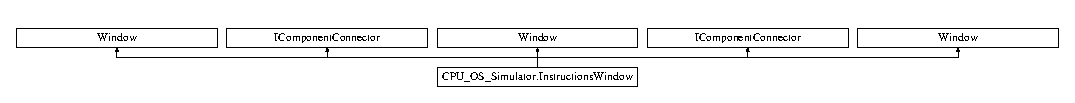
\includegraphics[height=0.929461cm]{class_c_p_u___o_s___simulator_1_1_instructions_window}
\end{center}
\end{figure}
\subsection*{Public Member Functions}
\begin{DoxyCompactItemize}
\item 
\hyperlink{class_c_p_u___o_s___simulator_1_1_instructions_window_aa482ef12f9c98458bedcc3c07d696879}{Instructions\+Window} ()
\begin{DoxyCompactList}\small\item\em Default Constructor for Instruction Window \end{DoxyCompactList}\item 
\hyperlink{class_c_p_u___o_s___simulator_1_1_instructions_window_a5ed238dc308dcc976400105a3973deb0}{Instructions\+Window} (\hyperlink{class_c_p_u___o_s___simulator_1_1_main_window}{Main\+Window} \hyperlink{class_c_p_u___o_s___simulator_1_1_instructions_window_a954c950c677c61a3b7ed7406b6dc7164}{owner})
\begin{DoxyCompactList}\small\item\em Constructor for instruction window that takes the window instance that is creating this window P\+L\+E\+A\+S\+E N\+O\+T\+E\+: This constructor should always be used so data can be passed back to the main window \end{DoxyCompactList}\item 
void \hyperlink{class_c_p_u___o_s___simulator_1_1_instructions_window_a8ad79899f3d5210d66fb5973b721895a}{Initialize\+Component} ()
\begin{DoxyCompactList}\small\item\em Initialize\+Component \end{DoxyCompactList}\item 
void \hyperlink{class_c_p_u___o_s___simulator_1_1_instructions_window_a8ad79899f3d5210d66fb5973b721895a}{Initialize\+Component} ()
\begin{DoxyCompactList}\small\item\em Initialize\+Component \end{DoxyCompactList}\end{DoxyCompactItemize}
\subsection*{Package Attributes}
\begin{DoxyCompactItemize}
\item 
\hyperlink{class_c_p_u___o_s___simulator_1_1_instructions_window}{C\+P\+U\+\_\+\+O\+S\+\_\+\+Simulator.\+Instructions\+Window} \hyperlink{class_c_p_u___o_s___simulator_1_1_instructions_window_ab7cd84f5ba064256327f6b1b1cdbc525}{Instructions\+Window1}
\item 
System.\+Windows.\+Controls.\+Grid \hyperlink{class_c_p_u___o_s___simulator_1_1_instructions_window_a83e86d19573c6c56db33e047354169a1}{grid\+\_\+\+Main}
\item 
System.\+Windows.\+Controls.\+Tab\+Control \hyperlink{class_c_p_u___o_s___simulator_1_1_instructions_window_a2e3784c64a40e14586270c1ebfe8bf3d}{Instruction\+Tabs}
\item 
System.\+Windows.\+Controls.\+Tab\+Item \hyperlink{class_c_p_u___o_s___simulator_1_1_instructions_window_a1076ccccc5b00e3f34ad487bc99b509b}{Data\+Transfer\+Tab}
\item 
System.\+Windows.\+Controls.\+Grid \hyperlink{class_c_p_u___o_s___simulator_1_1_instructions_window_a8e5436d90df63837c7f39586855bda1b}{Tab\+Grid}
\item 
System.\+Windows.\+Controls.\+Label \hyperlink{class_c_p_u___o_s___simulator_1_1_instructions_window_a71ce6968170dda46d83aefc71b63a96d}{label}
\item 
System.\+Windows.\+Controls.\+Grid \hyperlink{class_c_p_u___o_s___simulator_1_1_instructions_window_af568f7891b3381f9bec2f0d5b2d0d8c6}{Instruction\+List\+Grid}
\item 
System.\+Windows.\+Controls.\+List\+Box \hyperlink{class_c_p_u___o_s___simulator_1_1_instructions_window_a03052f893a09b459e840597cf98baffc}{lst\+\_\+\+Opcode\+List\+Data\+Transfer}
\item 
System.\+Windows.\+Controls.\+Grid \hyperlink{class_c_p_u___o_s___simulator_1_1_instructions_window_a6e37ff7da499bab3f5b0037d2b4c68cd}{Source\+Operand\+Grid}
\item 
System.\+Windows.\+Controls.\+Group\+Box \hyperlink{class_c_p_u___o_s___simulator_1_1_instructions_window_ace26d2d0e3de3715d755e91ab04a054a}{grp\+\_\+\+Source\+Operand}
\item 
System.\+Windows.\+Controls.\+Radio\+Button \hyperlink{class_c_p_u___o_s___simulator_1_1_instructions_window_a0798a7bfaace0c96650cf9df53fbf6fd}{rdb\+\_\+\+Source\+Value\+Data\+Transfer}
\item 
System.\+Windows.\+Controls.\+Text\+Box \hyperlink{class_c_p_u___o_s___simulator_1_1_instructions_window_a44cd8a2732d939d1746051f8b2093500}{txt\+Source\+Value\+Data\+Transfer}
\item 
System.\+Windows.\+Controls.\+Radio\+Button \hyperlink{class_c_p_u___o_s___simulator_1_1_instructions_window_a0d449427537f2c5baea2e2b7e669a9d7}{rdb\+\_\+\+Source\+Register\+Data\+Transfer}
\item 
System.\+Windows.\+Controls.\+Combo\+Box \hyperlink{class_c_p_u___o_s___simulator_1_1_instructions_window_ae2136d0a711f92a681278571fbe2868b}{cmb\+\_\+\+Source\+Register\+Data\+Transfer}
\item 
System.\+Windows.\+Controls.\+Grid \hyperlink{class_c_p_u___o_s___simulator_1_1_instructions_window_a46fbe457dccbe131387644a73cc19b19}{Source\+Operand\+Grid\+\_\+\+Copy}
\item 
System.\+Windows.\+Controls.\+Group\+Box \hyperlink{class_c_p_u___o_s___simulator_1_1_instructions_window_a836175caed2a6d02d8635bb6cc3f6cae}{grp\+\_\+\+Destination\+Operand}
\item 
System.\+Windows.\+Controls.\+Radio\+Button \hyperlink{class_c_p_u___o_s___simulator_1_1_instructions_window_a03ff2485a6554464a5c6c2b012dafd1a}{rdb\+\_\+\+Destination\+Value\+Data\+Transfer}
\item 
System.\+Windows.\+Controls.\+Text\+Box \hyperlink{class_c_p_u___o_s___simulator_1_1_instructions_window_a84f7cc6d64bd8050be7c729f469cd29c}{txt\+Destination\+Value\+Data\+Transfer}
\item 
System.\+Windows.\+Controls.\+Radio\+Button \hyperlink{class_c_p_u___o_s___simulator_1_1_instructions_window_a00e9e3013355f592d97a38b29e94899c}{rdb\+\_\+\+Destination\+Register\+Data\+Transfer}
\item 
System.\+Windows.\+Controls.\+Combo\+Box \hyperlink{class_c_p_u___o_s___simulator_1_1_instructions_window_a2cf44cbfe54b2d8f024d5c06067320a1}{cmb\+\_\+\+Destination\+Register\+Data\+Transfer}
\item 
System.\+Windows.\+Controls.\+Text\+Box \hyperlink{class_c_p_u___o_s___simulator_1_1_instructions_window_a58152c12c2022edc73b39c1f95ec7ba4}{txt\+Description\+Data\+Transfer}
\item 
System.\+Windows.\+Controls.\+Tab\+Item \hyperlink{class_c_p_u___o_s___simulator_1_1_instructions_window_a06c53026f495bcbdad82e84bbcb6611c}{Logical\+Tab}
\item 
System.\+Windows.\+Controls.\+Grid \hyperlink{class_c_p_u___o_s___simulator_1_1_instructions_window_a0f8731825bc5369e0328b2b9580e9b67}{Tab\+Grid\+\_\+\+Copy}
\item 
System.\+Windows.\+Controls.\+Label \hyperlink{class_c_p_u___o_s___simulator_1_1_instructions_window_a499640eb8a98693f1833dad30f5d8cb4}{label1}
\item 
System.\+Windows.\+Controls.\+Grid \hyperlink{class_c_p_u___o_s___simulator_1_1_instructions_window_a8f09b0005016c225169d7e9dd2724053}{Instruction\+List\+Grid1}
\item 
System.\+Windows.\+Controls.\+List\+Box \hyperlink{class_c_p_u___o_s___simulator_1_1_instructions_window_a61ee2cb0ba7197963b1138848778cd3c}{lst\+\_\+\+Opcode\+List\+Logical}
\item 
System.\+Windows.\+Controls.\+Grid \hyperlink{class_c_p_u___o_s___simulator_1_1_instructions_window_a3f9d1afc4455fa6b06c6fab3cdb6aeec}{Source\+Operand\+Grid1}
\item 
System.\+Windows.\+Controls.\+Group\+Box \hyperlink{class_c_p_u___o_s___simulator_1_1_instructions_window_a74e13776576d1a6ee5767e3fc8f6ec7f}{grp\+\_\+\+Source\+Operand1}
\item 
System.\+Windows.\+Controls.\+Radio\+Button \hyperlink{class_c_p_u___o_s___simulator_1_1_instructions_window_ad0e882b0d6d067460309ae6f1dda5d56}{rdb\+\_\+\+Source\+Value\+Logical}
\item 
System.\+Windows.\+Controls.\+Text\+Box \hyperlink{class_c_p_u___o_s___simulator_1_1_instructions_window_afac2309550dd6f1f1589dc7451e8f878}{txt\+Source\+Value\+Logical}
\item 
System.\+Windows.\+Controls.\+Radio\+Button \hyperlink{class_c_p_u___o_s___simulator_1_1_instructions_window_ab8c8622e8a96238fb88e455d60c51e78}{rdb\+\_\+\+Source\+Register\+Logical}
\item 
System.\+Windows.\+Controls.\+Combo\+Box \hyperlink{class_c_p_u___o_s___simulator_1_1_instructions_window_a46a9647a5a6e661afb789b1faa95a15a}{cmb\+\_\+\+Source\+Register\+Logical}
\item 
System.\+Windows.\+Controls.\+Grid \hyperlink{class_c_p_u___o_s___simulator_1_1_instructions_window_a685393ff28189e8c998e2a7dc6018b32}{Source\+Operand\+Grid\+\_\+\+Copy1}
\item 
System.\+Windows.\+Controls.\+Group\+Box \hyperlink{class_c_p_u___o_s___simulator_1_1_instructions_window_ab89f01ff39ce6f5ed461fcf5242be3a5}{grp\+\_\+\+Destination\+Operand1}
\item 
System.\+Windows.\+Controls.\+Radio\+Button \hyperlink{class_c_p_u___o_s___simulator_1_1_instructions_window_a73ba820a305842d3dea1ad79e6e87e6d}{rdb\+\_\+\+Destination\+Value\+Logical}
\item 
System.\+Windows.\+Controls.\+Text\+Box \hyperlink{class_c_p_u___o_s___simulator_1_1_instructions_window_af1a2860f125c3a8e25c73c1b04290438}{txt\+Destination\+Value\+Logical}
\item 
System.\+Windows.\+Controls.\+Radio\+Button \hyperlink{class_c_p_u___o_s___simulator_1_1_instructions_window_a3670f5971b586bd8977a78bcde185a35}{rdb\+\_\+\+Destination\+Register\+Logical}
\item 
System.\+Windows.\+Controls.\+Combo\+Box \hyperlink{class_c_p_u___o_s___simulator_1_1_instructions_window_aefcd87b5db00ac68e7d80ac5fddce8c5}{cmb\+\_\+\+Destination\+Register\+Logical}
\item 
System.\+Windows.\+Controls.\+Text\+Box \hyperlink{class_c_p_u___o_s___simulator_1_1_instructions_window_ae465810d61bb136b7934563cf85b3027}{txt\+Description\+Logical}
\item 
System.\+Windows.\+Controls.\+Tab\+Item \hyperlink{class_c_p_u___o_s___simulator_1_1_instructions_window_aabf61d7cbf8be85bb4ab0ef2d0614b46}{Arithmetic\+Tab}
\item 
System.\+Windows.\+Controls.\+Grid \hyperlink{class_c_p_u___o_s___simulator_1_1_instructions_window_a834965d0ae6a57edb71a818dca188a30}{Tab\+Grid\+\_\+\+Copy1}
\item 
System.\+Windows.\+Controls.\+Label \hyperlink{class_c_p_u___o_s___simulator_1_1_instructions_window_a237621e58e68c4a07cdf8803cc1614fd}{label2}
\item 
System.\+Windows.\+Controls.\+Grid \hyperlink{class_c_p_u___o_s___simulator_1_1_instructions_window_a33108da9779c5108fc5dd303a8d33454}{Instruction\+List\+Grid2}
\item 
System.\+Windows.\+Controls.\+List\+Box \hyperlink{class_c_p_u___o_s___simulator_1_1_instructions_window_a7445b276d3723f67ba564038940d44c5}{lst\+\_\+\+Opcode\+List\+Arithmetic}
\item 
System.\+Windows.\+Controls.\+Grid \hyperlink{class_c_p_u___o_s___simulator_1_1_instructions_window_a715ed01337540f316f39fe42c373c602}{Source\+Operand\+Grid2}
\item 
System.\+Windows.\+Controls.\+Group\+Box \hyperlink{class_c_p_u___o_s___simulator_1_1_instructions_window_ad37aae3614abd76749236a7739fbc18b}{grp\+\_\+\+Source\+Operand2}
\item 
System.\+Windows.\+Controls.\+Radio\+Button \hyperlink{class_c_p_u___o_s___simulator_1_1_instructions_window_a627e9cbe7e0cb2ce0f109f2345e19b73}{rdb\+\_\+\+Source\+Value\+Arithmetic}
\item 
System.\+Windows.\+Controls.\+Text\+Box \hyperlink{class_c_p_u___o_s___simulator_1_1_instructions_window_afc01788dc74f761b6cce800975394d2e}{txt\+Source\+Value\+Arithmetic}
\item 
System.\+Windows.\+Controls.\+Radio\+Button \hyperlink{class_c_p_u___o_s___simulator_1_1_instructions_window_ad571b65d5fe87bdb079c807dcac0680f}{rdb\+\_\+\+Source\+Register\+Arithmetic}
\item 
System.\+Windows.\+Controls.\+Combo\+Box \hyperlink{class_c_p_u___o_s___simulator_1_1_instructions_window_aad493dd174601ec265d5ad261f33d525}{cmb\+\_\+\+Source\+Register\+Arithmetic}
\item 
System.\+Windows.\+Controls.\+Grid \hyperlink{class_c_p_u___o_s___simulator_1_1_instructions_window_a6a57e0ae92b85cd619ef3d879ef0c628}{Source\+Operand\+Grid\+\_\+\+Copy2}
\item 
System.\+Windows.\+Controls.\+Group\+Box \hyperlink{class_c_p_u___o_s___simulator_1_1_instructions_window_adc32bbf0f47985507d606abb4862072f}{grp\+\_\+\+Destination\+Operand2}
\item 
System.\+Windows.\+Controls.\+Radio\+Button \hyperlink{class_c_p_u___o_s___simulator_1_1_instructions_window_a2e87a90d55ec015190b55bd06c273efc}{rdb\+\_\+\+Destination\+Value\+Arithmetic}
\item 
System.\+Windows.\+Controls.\+Text\+Box \hyperlink{class_c_p_u___o_s___simulator_1_1_instructions_window_adac073cb591b15be22d041695ff498e4}{txt\+Destination\+Value\+Arithmetic}
\item 
System.\+Windows.\+Controls.\+Radio\+Button \hyperlink{class_c_p_u___o_s___simulator_1_1_instructions_window_a40ebdc8941fbd7ae75ca6d14d1153569}{rdb\+\_\+\+Destination\+Register\+Arithmetic}
\item 
System.\+Windows.\+Controls.\+Combo\+Box \hyperlink{class_c_p_u___o_s___simulator_1_1_instructions_window_ad1fafd2bef9ad3f94fab585ea58fc38c}{cmb\+\_\+\+Destination\+Register\+Arithmetic}
\item 
System.\+Windows.\+Controls.\+Text\+Box \hyperlink{class_c_p_u___o_s___simulator_1_1_instructions_window_a31ef64d4c64f9791d6b4aad95cd4d95f}{txt\+Description\+Arithmetic}
\item 
System.\+Windows.\+Controls.\+Tab\+Item \hyperlink{class_c_p_u___o_s___simulator_1_1_instructions_window_a52cb165b57f01928c088b3052de70b5b}{Control\+Tranfer\+Tab}
\item 
System.\+Windows.\+Controls.\+Grid \hyperlink{class_c_p_u___o_s___simulator_1_1_instructions_window_ac4b83982bf62dc5c0484ac2729167ba4}{Tab\+Grid\+\_\+\+Copy2}
\item 
System.\+Windows.\+Controls.\+Label \hyperlink{class_c_p_u___o_s___simulator_1_1_instructions_window_a394b28c312ae1a83128da41990fc5d32}{label3}
\item 
System.\+Windows.\+Controls.\+Grid \hyperlink{class_c_p_u___o_s___simulator_1_1_instructions_window_a3cc76cf3ae5c4155d0e30727eb357d12}{Instruction\+List\+Grid3}
\item 
System.\+Windows.\+Controls.\+List\+Box \hyperlink{class_c_p_u___o_s___simulator_1_1_instructions_window_a111f1ddd903fe40e0c83efeca42bdf51}{lst\+\_\+\+Opcode\+List\+Control\+Transfer}
\item 
System.\+Windows.\+Controls.\+Grid \hyperlink{class_c_p_u___o_s___simulator_1_1_instructions_window_ab8409532df6419d7f7ce0c3450807906}{Source\+Operand\+Grid3}
\item 
System.\+Windows.\+Controls.\+Group\+Box \hyperlink{class_c_p_u___o_s___simulator_1_1_instructions_window_a59e5e9da77976ce8f2d8a43528b98f63}{grp\+\_\+\+Source\+Operand3}
\item 
System.\+Windows.\+Controls.\+Radio\+Button \hyperlink{class_c_p_u___o_s___simulator_1_1_instructions_window_a590a2e5af41ea5cf215da3ff7dd1b20b}{rdb\+\_\+\+Source\+Value\+Control\+Transfer}
\item 
System.\+Windows.\+Controls.\+Text\+Box \hyperlink{class_c_p_u___o_s___simulator_1_1_instructions_window_a602831ff353007879c08b22d373a2ba5}{txt\+Source\+Value\+Control\+Transfer}
\item 
System.\+Windows.\+Controls.\+Radio\+Button \hyperlink{class_c_p_u___o_s___simulator_1_1_instructions_window_a63fea6d97a26f4ed71753209dac85d24}{rdb\+\_\+\+Source\+Register\+Control\+Transfer}
\item 
System.\+Windows.\+Controls.\+Combo\+Box \hyperlink{class_c_p_u___o_s___simulator_1_1_instructions_window_a652354e464657693cf70a292b3389626}{cmb\+\_\+\+Source\+Register\+Control\+Transfer}
\item 
System.\+Windows.\+Controls.\+Grid \hyperlink{class_c_p_u___o_s___simulator_1_1_instructions_window_ac37123264ae139f4abc30841da21cd23}{Source\+Operand\+Grid\+\_\+\+Copy3}
\item 
System.\+Windows.\+Controls.\+Group\+Box \hyperlink{class_c_p_u___o_s___simulator_1_1_instructions_window_a175eb53a0a0f48be4d8717f1e5a5942e}{grp\+\_\+\+Destination\+Operand3}
\item 
System.\+Windows.\+Controls.\+Radio\+Button \hyperlink{class_c_p_u___o_s___simulator_1_1_instructions_window_afedaca6e4102fbae9f5db622be1b839d}{rdb\+\_\+\+Destination\+Value\+Control\+Transfer}
\item 
System.\+Windows.\+Controls.\+Text\+Box \hyperlink{class_c_p_u___o_s___simulator_1_1_instructions_window_a0049dce789d892e6620158859bcf7057}{txt\+Destination\+Value\+Control\+Transfer}
\item 
System.\+Windows.\+Controls.\+Radio\+Button \hyperlink{class_c_p_u___o_s___simulator_1_1_instructions_window_a4911636b6e093aa89155a0f5db4b3118}{rdb\+\_\+\+Destination\+Register\+Control\+Transfer}
\item 
System.\+Windows.\+Controls.\+Combo\+Box \hyperlink{class_c_p_u___o_s___simulator_1_1_instructions_window_a9017d3508e5dde75eafec25e94611c97}{cmb\+\_\+\+Destination\+Register\+Control\+Transfer}
\item 
System.\+Windows.\+Controls.\+Text\+Box \hyperlink{class_c_p_u___o_s___simulator_1_1_instructions_window_af8667a9cb444eb6aaa84349fe194b853}{txt\+Description\+Control\+Transfer}
\item 
System.\+Windows.\+Controls.\+Tab\+Item \hyperlink{class_c_p_u___o_s___simulator_1_1_instructions_window_ab807abcf9c3955ae2ff78e1d667820b2}{Comparison\+Tab}
\item 
System.\+Windows.\+Controls.\+Grid \hyperlink{class_c_p_u___o_s___simulator_1_1_instructions_window_a8a50487f6e6acca8a58ffe218e32abe2}{Tab\+Grid\+\_\+\+Copy3}
\item 
System.\+Windows.\+Controls.\+Label \hyperlink{class_c_p_u___o_s___simulator_1_1_instructions_window_a6d028c99fa713c891d86c07ef46f083b}{label4}
\item 
System.\+Windows.\+Controls.\+Grid \hyperlink{class_c_p_u___o_s___simulator_1_1_instructions_window_a9cdd58a2e38d3f0b047b6eb64b43ea03}{Instruction\+List\+Grid4}
\item 
System.\+Windows.\+Controls.\+List\+Box \hyperlink{class_c_p_u___o_s___simulator_1_1_instructions_window_ae47949fa5657e55f8acd8e5b9cd204c0}{lst\+\_\+\+Opcode\+List\+Comparison}
\item 
System.\+Windows.\+Controls.\+Grid \hyperlink{class_c_p_u___o_s___simulator_1_1_instructions_window_ac28180235c174caa7a2870120a9258bb}{Source\+Operand\+Grid4}
\item 
System.\+Windows.\+Controls.\+Group\+Box \hyperlink{class_c_p_u___o_s___simulator_1_1_instructions_window_a0efec3cdad460e3596a699716e0a24e9}{grp\+\_\+\+Source\+Operand4}
\item 
System.\+Windows.\+Controls.\+Radio\+Button \hyperlink{class_c_p_u___o_s___simulator_1_1_instructions_window_a6232aa7952b3d4ea71c55eb14267f188}{rdb\+\_\+\+Source\+Value\+Comparison}
\item 
System.\+Windows.\+Controls.\+Text\+Box \hyperlink{class_c_p_u___o_s___simulator_1_1_instructions_window_a8dd17881b7fd4e1923899b5bcae171fc}{txt\+Source\+Value\+Comparison}
\item 
System.\+Windows.\+Controls.\+Radio\+Button \hyperlink{class_c_p_u___o_s___simulator_1_1_instructions_window_afa2620b93d7d354b0632d7c290022545}{rdb\+\_\+\+Source\+Register\+Comparison}
\item 
System.\+Windows.\+Controls.\+Combo\+Box \hyperlink{class_c_p_u___o_s___simulator_1_1_instructions_window_af7acb32053b1cf27ee94bbf47efc9fbe}{cmb\+\_\+\+Source\+Register\+Comparison}
\item 
System.\+Windows.\+Controls.\+Grid \hyperlink{class_c_p_u___o_s___simulator_1_1_instructions_window_aa8c70305e3c77644ac312df74b0696b7}{Source\+Operand\+Grid\+\_\+\+Copy4}
\item 
System.\+Windows.\+Controls.\+Group\+Box \hyperlink{class_c_p_u___o_s___simulator_1_1_instructions_window_a68c2f892a54f7826baacf9c828431fa8}{grp\+\_\+\+Destination\+Operand4}
\item 
System.\+Windows.\+Controls.\+Radio\+Button \hyperlink{class_c_p_u___o_s___simulator_1_1_instructions_window_a200445a2378fddf69041aecbbcdf68fb}{rdb\+\_\+\+Destination\+Value\+Comparison}
\item 
System.\+Windows.\+Controls.\+Text\+Box \hyperlink{class_c_p_u___o_s___simulator_1_1_instructions_window_ab44686bd174144a0c1042579d6665547}{txt\+Destination\+Value\+Comparison}
\item 
System.\+Windows.\+Controls.\+Radio\+Button \hyperlink{class_c_p_u___o_s___simulator_1_1_instructions_window_af5369f91639cf92cbb6bd89118d6e373}{rdb\+\_\+\+Destination\+Register\+Comparison}
\item 
System.\+Windows.\+Controls.\+Combo\+Box \hyperlink{class_c_p_u___o_s___simulator_1_1_instructions_window_af209ebdcd0b9ae6c267388b382dac245}{cmb\+\_\+\+Destination\+Register\+Comparison}
\item 
System.\+Windows.\+Controls.\+Text\+Box \hyperlink{class_c_p_u___o_s___simulator_1_1_instructions_window_a1ac2050428b5ece7f1f6791771e9cef6}{txt\+Description\+Comparison}
\item 
System.\+Windows.\+Controls.\+Tab\+Item \hyperlink{class_c_p_u___o_s___simulator_1_1_instructions_window_aaf736178464d8313c866ab6efeae19c5}{I\+O\+Tab}
\item 
System.\+Windows.\+Controls.\+Grid \hyperlink{class_c_p_u___o_s___simulator_1_1_instructions_window_a33c64471b02aed8597462149051c2b51}{Tab\+Grid\+\_\+\+Copy4}
\item 
System.\+Windows.\+Controls.\+Label \hyperlink{class_c_p_u___o_s___simulator_1_1_instructions_window_acfbda3e1b251a166abc72a07d4cb5025}{label5}
\item 
System.\+Windows.\+Controls.\+Grid \hyperlink{class_c_p_u___o_s___simulator_1_1_instructions_window_a335e8ec02a78ffc483900745de96b602}{Instruction\+List\+Grid5}
\item 
System.\+Windows.\+Controls.\+List\+Box \hyperlink{class_c_p_u___o_s___simulator_1_1_instructions_window_aa8ccd453237503f0e15aff22975cea68}{lst\+\_\+\+Opcode\+List\+I\+O}
\item 
System.\+Windows.\+Controls.\+Grid \hyperlink{class_c_p_u___o_s___simulator_1_1_instructions_window_a3066f4664c81bacc6decdf84d08e74a9}{Source\+Operand\+Grid5}
\item 
System.\+Windows.\+Controls.\+Group\+Box \hyperlink{class_c_p_u___o_s___simulator_1_1_instructions_window_ab16ea5f8e2e761d0a7a0fe7054dfa3b5}{grp\+\_\+\+Source\+Operand5}
\item 
System.\+Windows.\+Controls.\+Radio\+Button \hyperlink{class_c_p_u___o_s___simulator_1_1_instructions_window_ad7bb114a6f948e79e55a44943ecf660a}{rdb\+\_\+\+Source\+Value\+I\+O}
\item 
System.\+Windows.\+Controls.\+Text\+Box \hyperlink{class_c_p_u___o_s___simulator_1_1_instructions_window_a14161b7bebd71e7545b59f77f6254a26}{txt\+Source\+Value\+I\+O}
\item 
System.\+Windows.\+Controls.\+Radio\+Button \hyperlink{class_c_p_u___o_s___simulator_1_1_instructions_window_a30064f400e25a6b155a34108a3fba816}{rdb\+\_\+\+Source\+Register\+I\+O}
\item 
System.\+Windows.\+Controls.\+Combo\+Box \hyperlink{class_c_p_u___o_s___simulator_1_1_instructions_window_a9f9d831a77d174675da89b1fe03602ad}{cmb\+\_\+\+Source\+Register\+I\+O}
\item 
System.\+Windows.\+Controls.\+Grid \hyperlink{class_c_p_u___o_s___simulator_1_1_instructions_window_a5a43b8933f014dffe28d3aa610518a94}{Source\+Operand\+Grid\+\_\+\+Copy5}
\item 
System.\+Windows.\+Controls.\+Group\+Box \hyperlink{class_c_p_u___o_s___simulator_1_1_instructions_window_aa99ecad0d35bc5e70a8924c9b3913106}{grp\+\_\+\+Destination\+Operand5}
\item 
System.\+Windows.\+Controls.\+Radio\+Button \hyperlink{class_c_p_u___o_s___simulator_1_1_instructions_window_a012739d419d605946f5dc0fd645db182}{rdb\+\_\+\+Destination\+Value\+I\+O}
\item 
System.\+Windows.\+Controls.\+Text\+Box \hyperlink{class_c_p_u___o_s___simulator_1_1_instructions_window_afd9084fd83f0c60a4fa1bba1cbcaf5af}{txt\+Destination\+Value\+I\+O}
\item 
System.\+Windows.\+Controls.\+Radio\+Button \hyperlink{class_c_p_u___o_s___simulator_1_1_instructions_window_a507ebe0998697ce8b2345fac2d9498a1}{rdb\+\_\+\+Destination\+Register\+I\+O}
\item 
System.\+Windows.\+Controls.\+Combo\+Box \hyperlink{class_c_p_u___o_s___simulator_1_1_instructions_window_a821452c6d5ab7be60996d3171a2d4cf1}{cmb\+\_\+\+Destination\+Register\+I\+O}
\item 
System.\+Windows.\+Controls.\+Text\+Box \hyperlink{class_c_p_u___o_s___simulator_1_1_instructions_window_a278020eeca6ae302ab5530cca856acde}{txt\+Description\+I\+O}
\item 
System.\+Windows.\+Controls.\+Tab\+Item \hyperlink{class_c_p_u___o_s___simulator_1_1_instructions_window_ab7e1bbdc8bb2830d39fb9a4339aa27f2}{Miscellaneous\+Tab}
\item 
System.\+Windows.\+Controls.\+Grid \hyperlink{class_c_p_u___o_s___simulator_1_1_instructions_window_a495a21e0e96f26f87d3e379ab286256b}{Tab\+Grid\+\_\+\+Copy5}
\item 
System.\+Windows.\+Controls.\+Label \hyperlink{class_c_p_u___o_s___simulator_1_1_instructions_window_a23cbea70a5e1ab92348a9569f362db07}{label6}
\item 
System.\+Windows.\+Controls.\+Grid \hyperlink{class_c_p_u___o_s___simulator_1_1_instructions_window_a6c86a044f242ee64f312f0105bac6d36}{Instruction\+List\+Grid6}
\item 
System.\+Windows.\+Controls.\+List\+Box \hyperlink{class_c_p_u___o_s___simulator_1_1_instructions_window_a3ac59be147d3323d2b485551b3a3640a}{lst\+\_\+\+Opcode\+List\+Miscellaneous}
\item 
System.\+Windows.\+Controls.\+Grid \hyperlink{class_c_p_u___o_s___simulator_1_1_instructions_window_a1036ae92003998bc7e7062a73358adec}{Source\+Operand\+Grid6}
\item 
System.\+Windows.\+Controls.\+Group\+Box \hyperlink{class_c_p_u___o_s___simulator_1_1_instructions_window_a46c1f50385d01108637e574343a99bfd}{grp\+\_\+\+Source\+Operand6}
\item 
System.\+Windows.\+Controls.\+Radio\+Button \hyperlink{class_c_p_u___o_s___simulator_1_1_instructions_window_ae6e33f7879251b63282f5d3eaa693507}{rdb\+\_\+\+Source\+Value\+Miscellaneous}
\item 
System.\+Windows.\+Controls.\+Text\+Box \hyperlink{class_c_p_u___o_s___simulator_1_1_instructions_window_a555d604d5869d89442a35900abc35914}{txt\+Source\+Value\+Miscellaneous}
\item 
System.\+Windows.\+Controls.\+Radio\+Button \hyperlink{class_c_p_u___o_s___simulator_1_1_instructions_window_ad2b0098ef721214b53b9e3241e611a84}{rdb\+\_\+\+Source\+Register\+Miscellaneous}
\item 
System.\+Windows.\+Controls.\+Combo\+Box \hyperlink{class_c_p_u___o_s___simulator_1_1_instructions_window_a98245ef6ca4796b7f59fe4b9937a388e}{cmb\+\_\+\+Source\+Register\+Miscellaneous}
\item 
System.\+Windows.\+Controls.\+Grid \hyperlink{class_c_p_u___o_s___simulator_1_1_instructions_window_a3dfdd68ad6b08fb1612fd43a420e5193}{Source\+Operand\+Grid\+\_\+\+Copy6}
\item 
System.\+Windows.\+Controls.\+Group\+Box \hyperlink{class_c_p_u___o_s___simulator_1_1_instructions_window_a8e457b3503625b5e837320ad9eb439c6}{grp\+\_\+\+Destination\+Operand6}
\item 
System.\+Windows.\+Controls.\+Radio\+Button \hyperlink{class_c_p_u___o_s___simulator_1_1_instructions_window_a567c8bba810d30e3c382e527e132a230}{rdb\+\_\+\+Destination\+Value\+Miscellaneous}
\item 
System.\+Windows.\+Controls.\+Text\+Box \hyperlink{class_c_p_u___o_s___simulator_1_1_instructions_window_a7fa1615bacb3264ac8ce61787a28d477}{txt\+Destination\+Value\+Miscellaneous}
\item 
System.\+Windows.\+Controls.\+Radio\+Button \hyperlink{class_c_p_u___o_s___simulator_1_1_instructions_window_adc4aa664244631ae1240a81d5c3b8ab5}{rdb\+\_\+\+Destination\+Register\+Miscellaneous}
\item 
System.\+Windows.\+Controls.\+Combo\+Box \hyperlink{class_c_p_u___o_s___simulator_1_1_instructions_window_ac4dab6ef32a46a295d6937b6bbda7813}{cmb\+\_\+\+Destination\+Register\+Miscellaneous}
\item 
System.\+Windows.\+Controls.\+Text\+Box \hyperlink{class_c_p_u___o_s___simulator_1_1_instructions_window_aaf938911ac6e23d7d637245cf40e6cbe}{txt\+Description\+Miscellaneous}
\item 
System.\+Windows.\+Controls.\+Button \hyperlink{class_c_p_u___o_s___simulator_1_1_instructions_window_a06305ca0735ae2d93a331fb33d2fe88f}{btn\+\_\+\+Close}
\end{DoxyCompactItemize}
\subsection*{Private Member Functions}
\begin{DoxyCompactItemize}
\item 
void \hyperlink{class_c_p_u___o_s___simulator_1_1_instructions_window_a52685f2ecc3d1cf7216716401d2621e0}{Populate\+Instructions} ()
\begin{DoxyCompactList}\small\item\em this function populates each of the instruction list boxes with the correct instructions \end{DoxyCompactList}\item 
void \hyperlink{class_c_p_u___o_s___simulator_1_1_instructions_window_a5fd3510dda95cf73b61af11ccacd81cd}{btn\+\_\+\+Close\+\_\+\+Click} (object sender, Routed\+Event\+Args e)
\begin{DoxyCompactList}\small\item\em This event handler is called when the close button is clicked \end{DoxyCompactList}\item 
void \hyperlink{class_c_p_u___o_s___simulator_1_1_instructions_window_a7d985ca63f2e27bc03a2198ec6879b49}{Window\+\_\+\+Loaded} (object sender, Routed\+Event\+Args e)
\begin{DoxyCompactList}\small\item\em This event handler is called when the window first loads \end{DoxyCompactList}\item 
void \hyperlink{class_c_p_u___o_s___simulator_1_1_instructions_window_a380aec4afa9900f7dd9ef964a5b86503}{lst\+\_\+\+Opcode\+List\+Data\+Transfer\+\_\+\+Selection\+Changed} (object sender, Selection\+Changed\+Event\+Args e)
\item 
void \hyperlink{class_c_p_u___o_s___simulator_1_1_instructions_window_a245baef3e788a01e6cf752f2c48f1843}{lst\+\_\+\+Opcode\+List\+Logical\+\_\+\+Selection\+Changed} (object sender, Selection\+Changed\+Event\+Args e)
\item 
void \hyperlink{class_c_p_u___o_s___simulator_1_1_instructions_window_ab4001352180ad08e3b335bf80c7dd9b8}{lst\+\_\+\+Opcode\+List\+Arithmetic\+\_\+\+Selection\+Changed} (object sender, Selection\+Changed\+Event\+Args e)
\item 
void \hyperlink{class_c_p_u___o_s___simulator_1_1_instructions_window_ac5b4dea0d3fe645b7f0bf9201cb0ad1c}{Instructions\+Window1\+\_\+\+Closing} (object sender, Cancel\+Event\+Args e)
\begin{DoxyCompactList}\small\item\em This event handler is called when the window is closing \end{DoxyCompactList}\item 
\hyperlink{class_c_p_u___o_s___simulator_1_1_c_p_u_1_1_register}{Register} \hyperlink{class_c_p_u___o_s___simulator_1_1_instructions_window_a2fbd163f2638a32f7cfbf831dc91582f}{Find\+Register} (string selected\+Item)
\begin{DoxyCompactList}\small\item\em Finds the register object for the selected register \end{DoxyCompactList}\item 
void \hyperlink{class_c_p_u___o_s___simulator_1_1_instructions_window_adce5e32de39213723ea06d279681b8ea}{rdb\+\_\+\+Source\+Value\+Data\+Transfer\+\_\+\+Checked} (object sender, Routed\+Event\+Args e)
\item 
void \hyperlink{class_c_p_u___o_s___simulator_1_1_instructions_window_aec7d6be51c8cd95dce4db01a5c66047e}{rdb\+\_\+\+Source\+Register\+Data\+Transfer\+\_\+\+Checked} (object sender, Routed\+Event\+Args e)
\item 
void \hyperlink{class_c_p_u___o_s___simulator_1_1_instructions_window_a8572bfa72449f43f800dd55961ad7837}{rdb\+\_\+\+Destination\+Value\+Data\+Transfer\+\_\+\+Checked} (object sender, Routed\+Event\+Args e)
\item 
void \hyperlink{class_c_p_u___o_s___simulator_1_1_instructions_window_a61a12a00e2f822ca948b2216b5dd85db}{rdb\+\_\+\+Destination\+Register\+Data\+Transfer\+\_\+\+Checked} (object sender, Routed\+Event\+Args e)
\item 
void System.\+Windows.\+Markup.\+I\+Component\+Connector. \hyperlink{class_c_p_u___o_s___simulator_1_1_instructions_window_a0efa7624a59a6abc64d0940ffaa100b0}{Connect} (int connection\+Id, object target)
\item 
void System.\+Windows.\+Markup.\+I\+Component\+Connector. \hyperlink{class_c_p_u___o_s___simulator_1_1_instructions_window_a0efa7624a59a6abc64d0940ffaa100b0}{Connect} (int connection\+Id, object target)
\end{DoxyCompactItemize}
\subsection*{Private Attributes}
\begin{DoxyCompactItemize}
\item 
List$<$ string $>$ \hyperlink{class_c_p_u___o_s___simulator_1_1_instructions_window_a678ab4df2b78758142472eeed8c5d7ba}{instruction\+Descriptions} = new List$<$string$>$()
\begin{DoxyCompactList}\small\item\em List to hold the descriptions of each instruction \end{DoxyCompactList}\item 
\hyperlink{class_c_p_u___o_s___simulator_1_1_main_window}{Main\+Window} \hyperlink{class_c_p_u___o_s___simulator_1_1_instructions_window_a954c950c677c61a3b7ed7406b6dc7164}{owner}
\begin{DoxyCompactList}\small\item\em The window that owns this window \end{DoxyCompactList}\item 
bool \hyperlink{class_c_p_u___o_s___simulator_1_1_instructions_window_a7755282dffea134038e9e58c931dc297}{\+\_\+content\+Loaded}
\end{DoxyCompactItemize}


\subsection{Detailed Description}
Interaction logic for Instructions\+Window.\+xaml 

\hyperlink{class_c_p_u___o_s___simulator_1_1_instructions_window}{Instructions\+Window} 

Definition at line 23 of file Instructions\+Window.\+xaml.\+cs.



\subsection{Constructor \& Destructor Documentation}
\hypertarget{class_c_p_u___o_s___simulator_1_1_instructions_window_aa482ef12f9c98458bedcc3c07d696879}{}\index{C\+P\+U\+\_\+\+O\+S\+\_\+\+Simulator\+::\+Instructions\+Window@{C\+P\+U\+\_\+\+O\+S\+\_\+\+Simulator\+::\+Instructions\+Window}!Instructions\+Window@{Instructions\+Window}}
\index{Instructions\+Window@{Instructions\+Window}!C\+P\+U\+\_\+\+O\+S\+\_\+\+Simulator\+::\+Instructions\+Window@{C\+P\+U\+\_\+\+O\+S\+\_\+\+Simulator\+::\+Instructions\+Window}}
\subsubsection[{Instructions\+Window()}]{\setlength{\rightskip}{0pt plus 5cm}C\+P\+U\+\_\+\+O\+S\+\_\+\+Simulator.\+Instructions\+Window.\+Instructions\+Window (
\begin{DoxyParamCaption}
{}
\end{DoxyParamCaption}
)}\label{class_c_p_u___o_s___simulator_1_1_instructions_window_aa482ef12f9c98458bedcc3c07d696879}


Default Constructor for Instruction Window 



Definition at line 36 of file Instructions\+Window.\+xaml.\+cs.

\hypertarget{class_c_p_u___o_s___simulator_1_1_instructions_window_a5ed238dc308dcc976400105a3973deb0}{}\index{C\+P\+U\+\_\+\+O\+S\+\_\+\+Simulator\+::\+Instructions\+Window@{C\+P\+U\+\_\+\+O\+S\+\_\+\+Simulator\+::\+Instructions\+Window}!Instructions\+Window@{Instructions\+Window}}
\index{Instructions\+Window@{Instructions\+Window}!C\+P\+U\+\_\+\+O\+S\+\_\+\+Simulator\+::\+Instructions\+Window@{C\+P\+U\+\_\+\+O\+S\+\_\+\+Simulator\+::\+Instructions\+Window}}
\subsubsection[{Instructions\+Window(\+Main\+Window owner)}]{\setlength{\rightskip}{0pt plus 5cm}C\+P\+U\+\_\+\+O\+S\+\_\+\+Simulator.\+Instructions\+Window.\+Instructions\+Window (
\begin{DoxyParamCaption}
\item[{{\bf Main\+Window}}]{owner}
\end{DoxyParamCaption}
)}\label{class_c_p_u___o_s___simulator_1_1_instructions_window_a5ed238dc308dcc976400105a3973deb0}


Constructor for instruction window that takes the window instance that is creating this window P\+L\+E\+A\+S\+E N\+O\+T\+E\+: This constructor should always be used so data can be passed back to the main window 


\begin{DoxyParams}{Parameters}
{\em owner} & The window that is creating this window \\
\hline
\end{DoxyParams}


Definition at line 45 of file Instructions\+Window.\+xaml.\+cs.



\subsection{Member Function Documentation}
\hypertarget{class_c_p_u___o_s___simulator_1_1_instructions_window_a5fd3510dda95cf73b61af11ccacd81cd}{}\index{C\+P\+U\+\_\+\+O\+S\+\_\+\+Simulator\+::\+Instructions\+Window@{C\+P\+U\+\_\+\+O\+S\+\_\+\+Simulator\+::\+Instructions\+Window}!btn\+\_\+\+Close\+\_\+\+Click@{btn\+\_\+\+Close\+\_\+\+Click}}
\index{btn\+\_\+\+Close\+\_\+\+Click@{btn\+\_\+\+Close\+\_\+\+Click}!C\+P\+U\+\_\+\+O\+S\+\_\+\+Simulator\+::\+Instructions\+Window@{C\+P\+U\+\_\+\+O\+S\+\_\+\+Simulator\+::\+Instructions\+Window}}
\subsubsection[{btn\+\_\+\+Close\+\_\+\+Click(object sender, Routed\+Event\+Args e)}]{\setlength{\rightskip}{0pt plus 5cm}void C\+P\+U\+\_\+\+O\+S\+\_\+\+Simulator.\+Instructions\+Window.\+btn\+\_\+\+Close\+\_\+\+Click (
\begin{DoxyParamCaption}
\item[{object}]{sender, }
\item[{Routed\+Event\+Args}]{e}
\end{DoxyParamCaption}
)\hspace{0.3cm}{\ttfamily [private]}}\label{class_c_p_u___o_s___simulator_1_1_instructions_window_a5fd3510dda95cf73b61af11ccacd81cd}


This event handler is called when the close button is clicked 


\begin{DoxyParams}{Parameters}
{\em sender} & the object that fired this event\\
\hline
{\em e} & the eventargs associated with this event\\
\hline
\end{DoxyParams}


Definition at line 96 of file Instructions\+Window.\+xaml.\+cs.

\hypertarget{class_c_p_u___o_s___simulator_1_1_instructions_window_a0efa7624a59a6abc64d0940ffaa100b0}{}\index{C\+P\+U\+\_\+\+O\+S\+\_\+\+Simulator\+::\+Instructions\+Window@{C\+P\+U\+\_\+\+O\+S\+\_\+\+Simulator\+::\+Instructions\+Window}!Connect@{Connect}}
\index{Connect@{Connect}!C\+P\+U\+\_\+\+O\+S\+\_\+\+Simulator\+::\+Instructions\+Window@{C\+P\+U\+\_\+\+O\+S\+\_\+\+Simulator\+::\+Instructions\+Window}}
\subsubsection[{Connect(int connection\+Id, object target)}]{\setlength{\rightskip}{0pt plus 5cm}void System.\+Windows.\+Markup.\+I\+Component\+Connector. C\+P\+U\+\_\+\+O\+S\+\_\+\+Simulator.\+Instructions\+Window.\+Connect (
\begin{DoxyParamCaption}
\item[{int}]{connection\+Id, }
\item[{object}]{target}
\end{DoxyParamCaption}
)\hspace{0.3cm}{\ttfamily [private]}}\label{class_c_p_u___o_s___simulator_1_1_instructions_window_a0efa7624a59a6abc64d0940ffaa100b0}


Definition at line 1110 of file Instructions\+Window.\+g.\+i.\+cs.

\hypertarget{class_c_p_u___o_s___simulator_1_1_instructions_window_a0efa7624a59a6abc64d0940ffaa100b0}{}\index{C\+P\+U\+\_\+\+O\+S\+\_\+\+Simulator\+::\+Instructions\+Window@{C\+P\+U\+\_\+\+O\+S\+\_\+\+Simulator\+::\+Instructions\+Window}!Connect@{Connect}}
\index{Connect@{Connect}!C\+P\+U\+\_\+\+O\+S\+\_\+\+Simulator\+::\+Instructions\+Window@{C\+P\+U\+\_\+\+O\+S\+\_\+\+Simulator\+::\+Instructions\+Window}}
\subsubsection[{Connect(int connection\+Id, object target)}]{\setlength{\rightskip}{0pt plus 5cm}void System.\+Windows.\+Markup.\+I\+Component\+Connector. C\+P\+U\+\_\+\+O\+S\+\_\+\+Simulator.\+Instructions\+Window.\+Connect (
\begin{DoxyParamCaption}
\item[{int}]{connection\+Id, }
\item[{object}]{target}
\end{DoxyParamCaption}
)\hspace{0.3cm}{\ttfamily [private]}}\label{class_c_p_u___o_s___simulator_1_1_instructions_window_a0efa7624a59a6abc64d0940ffaa100b0}


Definition at line 1110 of file Instructions\+Window.\+g.\+cs.

\hypertarget{class_c_p_u___o_s___simulator_1_1_instructions_window_a2fbd163f2638a32f7cfbf831dc91582f}{}\index{C\+P\+U\+\_\+\+O\+S\+\_\+\+Simulator\+::\+Instructions\+Window@{C\+P\+U\+\_\+\+O\+S\+\_\+\+Simulator\+::\+Instructions\+Window}!Find\+Register@{Find\+Register}}
\index{Find\+Register@{Find\+Register}!C\+P\+U\+\_\+\+O\+S\+\_\+\+Simulator\+::\+Instructions\+Window@{C\+P\+U\+\_\+\+O\+S\+\_\+\+Simulator\+::\+Instructions\+Window}}
\subsubsection[{Find\+Register(string selected\+Item)}]{\setlength{\rightskip}{0pt plus 5cm}{\bf Register} C\+P\+U\+\_\+\+O\+S\+\_\+\+Simulator.\+Instructions\+Window.\+Find\+Register (
\begin{DoxyParamCaption}
\item[{string}]{selected\+Item}
\end{DoxyParamCaption}
)\hspace{0.3cm}{\ttfamily [private]}}\label{class_c_p_u___o_s___simulator_1_1_instructions_window_a2fbd163f2638a32f7cfbf831dc91582f}


Finds the register object for the selected register 


\begin{DoxyParams}{Parameters}
{\em selected\+Item} & the selected register\\
\hline
\end{DoxyParams}
\begin{DoxyReturn}{Returns}
The register object of the selected register
\end{DoxyReturn}


Definition at line 176 of file Instructions\+Window.\+xaml.\+cs.

\hypertarget{class_c_p_u___o_s___simulator_1_1_instructions_window_a8ad79899f3d5210d66fb5973b721895a}{}\index{C\+P\+U\+\_\+\+O\+S\+\_\+\+Simulator\+::\+Instructions\+Window@{C\+P\+U\+\_\+\+O\+S\+\_\+\+Simulator\+::\+Instructions\+Window}!Initialize\+Component@{Initialize\+Component}}
\index{Initialize\+Component@{Initialize\+Component}!C\+P\+U\+\_\+\+O\+S\+\_\+\+Simulator\+::\+Instructions\+Window@{C\+P\+U\+\_\+\+O\+S\+\_\+\+Simulator\+::\+Instructions\+Window}}
\subsubsection[{Initialize\+Component()}]{\setlength{\rightskip}{0pt plus 5cm}void C\+P\+U\+\_\+\+O\+S\+\_\+\+Simulator.\+Instructions\+Window.\+Initialize\+Component (
\begin{DoxyParamCaption}
{}
\end{DoxyParamCaption}
)}\label{class_c_p_u___o_s___simulator_1_1_instructions_window_a8ad79899f3d5210d66fb5973b721895a}


Initialize\+Component 



Definition at line 1090 of file Instructions\+Window.\+g.\+i.\+cs.

\hypertarget{class_c_p_u___o_s___simulator_1_1_instructions_window_a8ad79899f3d5210d66fb5973b721895a}{}\index{C\+P\+U\+\_\+\+O\+S\+\_\+\+Simulator\+::\+Instructions\+Window@{C\+P\+U\+\_\+\+O\+S\+\_\+\+Simulator\+::\+Instructions\+Window}!Initialize\+Component@{Initialize\+Component}}
\index{Initialize\+Component@{Initialize\+Component}!C\+P\+U\+\_\+\+O\+S\+\_\+\+Simulator\+::\+Instructions\+Window@{C\+P\+U\+\_\+\+O\+S\+\_\+\+Simulator\+::\+Instructions\+Window}}
\subsubsection[{Initialize\+Component()}]{\setlength{\rightskip}{0pt plus 5cm}void C\+P\+U\+\_\+\+O\+S\+\_\+\+Simulator.\+Instructions\+Window.\+Initialize\+Component (
\begin{DoxyParamCaption}
{}
\end{DoxyParamCaption}
)}\label{class_c_p_u___o_s___simulator_1_1_instructions_window_a8ad79899f3d5210d66fb5973b721895a}


Initialize\+Component 



Definition at line 1090 of file Instructions\+Window.\+g.\+cs.

\hypertarget{class_c_p_u___o_s___simulator_1_1_instructions_window_ac5b4dea0d3fe645b7f0bf9201cb0ad1c}{}\index{C\+P\+U\+\_\+\+O\+S\+\_\+\+Simulator\+::\+Instructions\+Window@{C\+P\+U\+\_\+\+O\+S\+\_\+\+Simulator\+::\+Instructions\+Window}!Instructions\+Window1\+\_\+\+Closing@{Instructions\+Window1\+\_\+\+Closing}}
\index{Instructions\+Window1\+\_\+\+Closing@{Instructions\+Window1\+\_\+\+Closing}!C\+P\+U\+\_\+\+O\+S\+\_\+\+Simulator\+::\+Instructions\+Window@{C\+P\+U\+\_\+\+O\+S\+\_\+\+Simulator\+::\+Instructions\+Window}}
\subsubsection[{Instructions\+Window1\+\_\+\+Closing(object sender, Cancel\+Event\+Args e)}]{\setlength{\rightskip}{0pt plus 5cm}void C\+P\+U\+\_\+\+O\+S\+\_\+\+Simulator.\+Instructions\+Window.\+Instructions\+Window1\+\_\+\+Closing (
\begin{DoxyParamCaption}
\item[{object}]{sender, }
\item[{Cancel\+Event\+Args}]{e}
\end{DoxyParamCaption}
)\hspace{0.3cm}{\ttfamily [private]}}\label{class_c_p_u___o_s___simulator_1_1_instructions_window_ac5b4dea0d3fe645b7f0bf9201cb0ad1c}


This event handler is called when the window is closing 


\begin{DoxyParams}{Parameters}
{\em sender} & the object that fired this event\\
\hline
{\em e} & the eventargs associated with this event\\
\hline
\end{DoxyParams}


Definition at line 134 of file Instructions\+Window.\+xaml.\+cs.

\hypertarget{class_c_p_u___o_s___simulator_1_1_instructions_window_ab4001352180ad08e3b335bf80c7dd9b8}{}\index{C\+P\+U\+\_\+\+O\+S\+\_\+\+Simulator\+::\+Instructions\+Window@{C\+P\+U\+\_\+\+O\+S\+\_\+\+Simulator\+::\+Instructions\+Window}!lst\+\_\+\+Opcode\+List\+Arithmetic\+\_\+\+Selection\+Changed@{lst\+\_\+\+Opcode\+List\+Arithmetic\+\_\+\+Selection\+Changed}}
\index{lst\+\_\+\+Opcode\+List\+Arithmetic\+\_\+\+Selection\+Changed@{lst\+\_\+\+Opcode\+List\+Arithmetic\+\_\+\+Selection\+Changed}!C\+P\+U\+\_\+\+O\+S\+\_\+\+Simulator\+::\+Instructions\+Window@{C\+P\+U\+\_\+\+O\+S\+\_\+\+Simulator\+::\+Instructions\+Window}}
\subsubsection[{lst\+\_\+\+Opcode\+List\+Arithmetic\+\_\+\+Selection\+Changed(object sender, Selection\+Changed\+Event\+Args e)}]{\setlength{\rightskip}{0pt plus 5cm}void C\+P\+U\+\_\+\+O\+S\+\_\+\+Simulator.\+Instructions\+Window.\+lst\+\_\+\+Opcode\+List\+Arithmetic\+\_\+\+Selection\+Changed (
\begin{DoxyParamCaption}
\item[{object}]{sender, }
\item[{Selection\+Changed\+Event\+Args}]{e}
\end{DoxyParamCaption}
)\hspace{0.3cm}{\ttfamily [private]}}\label{class_c_p_u___o_s___simulator_1_1_instructions_window_ab4001352180ad08e3b335bf80c7dd9b8}


Definition at line 124 of file Instructions\+Window.\+xaml.\+cs.

\hypertarget{class_c_p_u___o_s___simulator_1_1_instructions_window_a380aec4afa9900f7dd9ef964a5b86503}{}\index{C\+P\+U\+\_\+\+O\+S\+\_\+\+Simulator\+::\+Instructions\+Window@{C\+P\+U\+\_\+\+O\+S\+\_\+\+Simulator\+::\+Instructions\+Window}!lst\+\_\+\+Opcode\+List\+Data\+Transfer\+\_\+\+Selection\+Changed@{lst\+\_\+\+Opcode\+List\+Data\+Transfer\+\_\+\+Selection\+Changed}}
\index{lst\+\_\+\+Opcode\+List\+Data\+Transfer\+\_\+\+Selection\+Changed@{lst\+\_\+\+Opcode\+List\+Data\+Transfer\+\_\+\+Selection\+Changed}!C\+P\+U\+\_\+\+O\+S\+\_\+\+Simulator\+::\+Instructions\+Window@{C\+P\+U\+\_\+\+O\+S\+\_\+\+Simulator\+::\+Instructions\+Window}}
\subsubsection[{lst\+\_\+\+Opcode\+List\+Data\+Transfer\+\_\+\+Selection\+Changed(object sender, Selection\+Changed\+Event\+Args e)}]{\setlength{\rightskip}{0pt plus 5cm}void C\+P\+U\+\_\+\+O\+S\+\_\+\+Simulator.\+Instructions\+Window.\+lst\+\_\+\+Opcode\+List\+Data\+Transfer\+\_\+\+Selection\+Changed (
\begin{DoxyParamCaption}
\item[{object}]{sender, }
\item[{Selection\+Changed\+Event\+Args}]{e}
\end{DoxyParamCaption}
)\hspace{0.3cm}{\ttfamily [private]}}\label{class_c_p_u___o_s___simulator_1_1_instructions_window_a380aec4afa9900f7dd9ef964a5b86503}


Definition at line 112 of file Instructions\+Window.\+xaml.\+cs.

\hypertarget{class_c_p_u___o_s___simulator_1_1_instructions_window_a245baef3e788a01e6cf752f2c48f1843}{}\index{C\+P\+U\+\_\+\+O\+S\+\_\+\+Simulator\+::\+Instructions\+Window@{C\+P\+U\+\_\+\+O\+S\+\_\+\+Simulator\+::\+Instructions\+Window}!lst\+\_\+\+Opcode\+List\+Logical\+\_\+\+Selection\+Changed@{lst\+\_\+\+Opcode\+List\+Logical\+\_\+\+Selection\+Changed}}
\index{lst\+\_\+\+Opcode\+List\+Logical\+\_\+\+Selection\+Changed@{lst\+\_\+\+Opcode\+List\+Logical\+\_\+\+Selection\+Changed}!C\+P\+U\+\_\+\+O\+S\+\_\+\+Simulator\+::\+Instructions\+Window@{C\+P\+U\+\_\+\+O\+S\+\_\+\+Simulator\+::\+Instructions\+Window}}
\subsubsection[{lst\+\_\+\+Opcode\+List\+Logical\+\_\+\+Selection\+Changed(object sender, Selection\+Changed\+Event\+Args e)}]{\setlength{\rightskip}{0pt plus 5cm}void C\+P\+U\+\_\+\+O\+S\+\_\+\+Simulator.\+Instructions\+Window.\+lst\+\_\+\+Opcode\+List\+Logical\+\_\+\+Selection\+Changed (
\begin{DoxyParamCaption}
\item[{object}]{sender, }
\item[{Selection\+Changed\+Event\+Args}]{e}
\end{DoxyParamCaption}
)\hspace{0.3cm}{\ttfamily [private]}}\label{class_c_p_u___o_s___simulator_1_1_instructions_window_a245baef3e788a01e6cf752f2c48f1843}


Definition at line 118 of file Instructions\+Window.\+xaml.\+cs.

\hypertarget{class_c_p_u___o_s___simulator_1_1_instructions_window_a52685f2ecc3d1cf7216716401d2621e0}{}\index{C\+P\+U\+\_\+\+O\+S\+\_\+\+Simulator\+::\+Instructions\+Window@{C\+P\+U\+\_\+\+O\+S\+\_\+\+Simulator\+::\+Instructions\+Window}!Populate\+Instructions@{Populate\+Instructions}}
\index{Populate\+Instructions@{Populate\+Instructions}!C\+P\+U\+\_\+\+O\+S\+\_\+\+Simulator\+::\+Instructions\+Window@{C\+P\+U\+\_\+\+O\+S\+\_\+\+Simulator\+::\+Instructions\+Window}}
\subsubsection[{Populate\+Instructions()}]{\setlength{\rightskip}{0pt plus 5cm}void C\+P\+U\+\_\+\+O\+S\+\_\+\+Simulator.\+Instructions\+Window.\+Populate\+Instructions (
\begin{DoxyParamCaption}
{}
\end{DoxyParamCaption}
)\hspace{0.3cm}{\ttfamily [private]}}\label{class_c_p_u___o_s___simulator_1_1_instructions_window_a52685f2ecc3d1cf7216716401d2621e0}


this function populates each of the instruction list boxes with the correct instructions 



Definition at line 54 of file Instructions\+Window.\+xaml.\+cs.

\hypertarget{class_c_p_u___o_s___simulator_1_1_instructions_window_a61a12a00e2f822ca948b2216b5dd85db}{}\index{C\+P\+U\+\_\+\+O\+S\+\_\+\+Simulator\+::\+Instructions\+Window@{C\+P\+U\+\_\+\+O\+S\+\_\+\+Simulator\+::\+Instructions\+Window}!rdb\+\_\+\+Destination\+Register\+Data\+Transfer\+\_\+\+Checked@{rdb\+\_\+\+Destination\+Register\+Data\+Transfer\+\_\+\+Checked}}
\index{rdb\+\_\+\+Destination\+Register\+Data\+Transfer\+\_\+\+Checked@{rdb\+\_\+\+Destination\+Register\+Data\+Transfer\+\_\+\+Checked}!C\+P\+U\+\_\+\+O\+S\+\_\+\+Simulator\+::\+Instructions\+Window@{C\+P\+U\+\_\+\+O\+S\+\_\+\+Simulator\+::\+Instructions\+Window}}
\subsubsection[{rdb\+\_\+\+Destination\+Register\+Data\+Transfer\+\_\+\+Checked(object sender, Routed\+Event\+Args e)}]{\setlength{\rightskip}{0pt plus 5cm}void C\+P\+U\+\_\+\+O\+S\+\_\+\+Simulator.\+Instructions\+Window.\+rdb\+\_\+\+Destination\+Register\+Data\+Transfer\+\_\+\+Checked (
\begin{DoxyParamCaption}
\item[{object}]{sender, }
\item[{Routed\+Event\+Args}]{e}
\end{DoxyParamCaption}
)\hspace{0.3cm}{\ttfamily [private]}}\label{class_c_p_u___o_s___simulator_1_1_instructions_window_a61a12a00e2f822ca948b2216b5dd85db}


Definition at line 217 of file Instructions\+Window.\+xaml.\+cs.

\hypertarget{class_c_p_u___o_s___simulator_1_1_instructions_window_a8572bfa72449f43f800dd55961ad7837}{}\index{C\+P\+U\+\_\+\+O\+S\+\_\+\+Simulator\+::\+Instructions\+Window@{C\+P\+U\+\_\+\+O\+S\+\_\+\+Simulator\+::\+Instructions\+Window}!rdb\+\_\+\+Destination\+Value\+Data\+Transfer\+\_\+\+Checked@{rdb\+\_\+\+Destination\+Value\+Data\+Transfer\+\_\+\+Checked}}
\index{rdb\+\_\+\+Destination\+Value\+Data\+Transfer\+\_\+\+Checked@{rdb\+\_\+\+Destination\+Value\+Data\+Transfer\+\_\+\+Checked}!C\+P\+U\+\_\+\+O\+S\+\_\+\+Simulator\+::\+Instructions\+Window@{C\+P\+U\+\_\+\+O\+S\+\_\+\+Simulator\+::\+Instructions\+Window}}
\subsubsection[{rdb\+\_\+\+Destination\+Value\+Data\+Transfer\+\_\+\+Checked(object sender, Routed\+Event\+Args e)}]{\setlength{\rightskip}{0pt plus 5cm}void C\+P\+U\+\_\+\+O\+S\+\_\+\+Simulator.\+Instructions\+Window.\+rdb\+\_\+\+Destination\+Value\+Data\+Transfer\+\_\+\+Checked (
\begin{DoxyParamCaption}
\item[{object}]{sender, }
\item[{Routed\+Event\+Args}]{e}
\end{DoxyParamCaption}
)\hspace{0.3cm}{\ttfamily [private]}}\label{class_c_p_u___o_s___simulator_1_1_instructions_window_a8572bfa72449f43f800dd55961ad7837}


Definition at line 210 of file Instructions\+Window.\+xaml.\+cs.

\hypertarget{class_c_p_u___o_s___simulator_1_1_instructions_window_aec7d6be51c8cd95dce4db01a5c66047e}{}\index{C\+P\+U\+\_\+\+O\+S\+\_\+\+Simulator\+::\+Instructions\+Window@{C\+P\+U\+\_\+\+O\+S\+\_\+\+Simulator\+::\+Instructions\+Window}!rdb\+\_\+\+Source\+Register\+Data\+Transfer\+\_\+\+Checked@{rdb\+\_\+\+Source\+Register\+Data\+Transfer\+\_\+\+Checked}}
\index{rdb\+\_\+\+Source\+Register\+Data\+Transfer\+\_\+\+Checked@{rdb\+\_\+\+Source\+Register\+Data\+Transfer\+\_\+\+Checked}!C\+P\+U\+\_\+\+O\+S\+\_\+\+Simulator\+::\+Instructions\+Window@{C\+P\+U\+\_\+\+O\+S\+\_\+\+Simulator\+::\+Instructions\+Window}}
\subsubsection[{rdb\+\_\+\+Source\+Register\+Data\+Transfer\+\_\+\+Checked(object sender, Routed\+Event\+Args e)}]{\setlength{\rightskip}{0pt plus 5cm}void C\+P\+U\+\_\+\+O\+S\+\_\+\+Simulator.\+Instructions\+Window.\+rdb\+\_\+\+Source\+Register\+Data\+Transfer\+\_\+\+Checked (
\begin{DoxyParamCaption}
\item[{object}]{sender, }
\item[{Routed\+Event\+Args}]{e}
\end{DoxyParamCaption}
)\hspace{0.3cm}{\ttfamily [private]}}\label{class_c_p_u___o_s___simulator_1_1_instructions_window_aec7d6be51c8cd95dce4db01a5c66047e}


Definition at line 202 of file Instructions\+Window.\+xaml.\+cs.

\hypertarget{class_c_p_u___o_s___simulator_1_1_instructions_window_adce5e32de39213723ea06d279681b8ea}{}\index{C\+P\+U\+\_\+\+O\+S\+\_\+\+Simulator\+::\+Instructions\+Window@{C\+P\+U\+\_\+\+O\+S\+\_\+\+Simulator\+::\+Instructions\+Window}!rdb\+\_\+\+Source\+Value\+Data\+Transfer\+\_\+\+Checked@{rdb\+\_\+\+Source\+Value\+Data\+Transfer\+\_\+\+Checked}}
\index{rdb\+\_\+\+Source\+Value\+Data\+Transfer\+\_\+\+Checked@{rdb\+\_\+\+Source\+Value\+Data\+Transfer\+\_\+\+Checked}!C\+P\+U\+\_\+\+O\+S\+\_\+\+Simulator\+::\+Instructions\+Window@{C\+P\+U\+\_\+\+O\+S\+\_\+\+Simulator\+::\+Instructions\+Window}}
\subsubsection[{rdb\+\_\+\+Source\+Value\+Data\+Transfer\+\_\+\+Checked(object sender, Routed\+Event\+Args e)}]{\setlength{\rightskip}{0pt plus 5cm}void C\+P\+U\+\_\+\+O\+S\+\_\+\+Simulator.\+Instructions\+Window.\+rdb\+\_\+\+Source\+Value\+Data\+Transfer\+\_\+\+Checked (
\begin{DoxyParamCaption}
\item[{object}]{sender, }
\item[{Routed\+Event\+Args}]{e}
\end{DoxyParamCaption}
)\hspace{0.3cm}{\ttfamily [private]}}\label{class_c_p_u___o_s___simulator_1_1_instructions_window_adce5e32de39213723ea06d279681b8ea}


Definition at line 195 of file Instructions\+Window.\+xaml.\+cs.

\hypertarget{class_c_p_u___o_s___simulator_1_1_instructions_window_a7d985ca63f2e27bc03a2198ec6879b49}{}\index{C\+P\+U\+\_\+\+O\+S\+\_\+\+Simulator\+::\+Instructions\+Window@{C\+P\+U\+\_\+\+O\+S\+\_\+\+Simulator\+::\+Instructions\+Window}!Window\+\_\+\+Loaded@{Window\+\_\+\+Loaded}}
\index{Window\+\_\+\+Loaded@{Window\+\_\+\+Loaded}!C\+P\+U\+\_\+\+O\+S\+\_\+\+Simulator\+::\+Instructions\+Window@{C\+P\+U\+\_\+\+O\+S\+\_\+\+Simulator\+::\+Instructions\+Window}}
\subsubsection[{Window\+\_\+\+Loaded(object sender, Routed\+Event\+Args e)}]{\setlength{\rightskip}{0pt plus 5cm}void C\+P\+U\+\_\+\+O\+S\+\_\+\+Simulator.\+Instructions\+Window.\+Window\+\_\+\+Loaded (
\begin{DoxyParamCaption}
\item[{object}]{sender, }
\item[{Routed\+Event\+Args}]{e}
\end{DoxyParamCaption}
)\hspace{0.3cm}{\ttfamily [private]}}\label{class_c_p_u___o_s___simulator_1_1_instructions_window_a7d985ca63f2e27bc03a2198ec6879b49}


This event handler is called when the window first loads 


\begin{DoxyParams}{Parameters}
{\em sender} & the object that fired this event\\
\hline
{\em e} & the eventargs associated with this event\\
\hline
\end{DoxyParams}


Definition at line 105 of file Instructions\+Window.\+xaml.\+cs.



\subsection{Member Data Documentation}
\hypertarget{class_c_p_u___o_s___simulator_1_1_instructions_window_a7755282dffea134038e9e58c931dc297}{}\index{C\+P\+U\+\_\+\+O\+S\+\_\+\+Simulator\+::\+Instructions\+Window@{C\+P\+U\+\_\+\+O\+S\+\_\+\+Simulator\+::\+Instructions\+Window}!\+\_\+content\+Loaded@{\+\_\+content\+Loaded}}
\index{\+\_\+content\+Loaded@{\+\_\+content\+Loaded}!C\+P\+U\+\_\+\+O\+S\+\_\+\+Simulator\+::\+Instructions\+Window@{C\+P\+U\+\_\+\+O\+S\+\_\+\+Simulator\+::\+Instructions\+Window}}
\subsubsection[{\+\_\+content\+Loaded}]{\setlength{\rightskip}{0pt plus 5cm}bool C\+P\+U\+\_\+\+O\+S\+\_\+\+Simulator.\+Instructions\+Window.\+\_\+content\+Loaded\hspace{0.3cm}{\ttfamily [private]}}\label{class_c_p_u___o_s___simulator_1_1_instructions_window_a7755282dffea134038e9e58c931dc297}


Definition at line 1083 of file Instructions\+Window.\+g.\+cs.

\hypertarget{class_c_p_u___o_s___simulator_1_1_instructions_window_aabf61d7cbf8be85bb4ab0ef2d0614b46}{}\index{C\+P\+U\+\_\+\+O\+S\+\_\+\+Simulator\+::\+Instructions\+Window@{C\+P\+U\+\_\+\+O\+S\+\_\+\+Simulator\+::\+Instructions\+Window}!Arithmetic\+Tab@{Arithmetic\+Tab}}
\index{Arithmetic\+Tab@{Arithmetic\+Tab}!C\+P\+U\+\_\+\+O\+S\+\_\+\+Simulator\+::\+Instructions\+Window@{C\+P\+U\+\_\+\+O\+S\+\_\+\+Simulator\+::\+Instructions\+Window}}
\subsubsection[{Arithmetic\+Tab}]{\setlength{\rightskip}{0pt plus 5cm}System Windows Controls Tab\+Item C\+P\+U\+\_\+\+O\+S\+\_\+\+Simulator.\+Instructions\+Window.\+Arithmetic\+Tab\hspace{0.3cm}{\ttfamily [package]}}\label{class_c_p_u___o_s___simulator_1_1_instructions_window_aabf61d7cbf8be85bb4ab0ef2d0614b46}


Definition at line 358 of file Instructions\+Window.\+g.\+cs.

\hypertarget{class_c_p_u___o_s___simulator_1_1_instructions_window_a06305ca0735ae2d93a331fb33d2fe88f}{}\index{C\+P\+U\+\_\+\+O\+S\+\_\+\+Simulator\+::\+Instructions\+Window@{C\+P\+U\+\_\+\+O\+S\+\_\+\+Simulator\+::\+Instructions\+Window}!btn\+\_\+\+Close@{btn\+\_\+\+Close}}
\index{btn\+\_\+\+Close@{btn\+\_\+\+Close}!C\+P\+U\+\_\+\+O\+S\+\_\+\+Simulator\+::\+Instructions\+Window@{C\+P\+U\+\_\+\+O\+S\+\_\+\+Simulator\+::\+Instructions\+Window}}
\subsubsection[{btn\+\_\+\+Close}]{\setlength{\rightskip}{0pt plus 5cm}System Windows Controls Button C\+P\+U\+\_\+\+O\+S\+\_\+\+Simulator.\+Instructions\+Window.\+btn\+\_\+\+Close\hspace{0.3cm}{\ttfamily [package]}}\label{class_c_p_u___o_s___simulator_1_1_instructions_window_a06305ca0735ae2d93a331fb33d2fe88f}


Definition at line 1078 of file Instructions\+Window.\+g.\+cs.

\hypertarget{class_c_p_u___o_s___simulator_1_1_instructions_window_ad1fafd2bef9ad3f94fab585ea58fc38c}{}\index{C\+P\+U\+\_\+\+O\+S\+\_\+\+Simulator\+::\+Instructions\+Window@{C\+P\+U\+\_\+\+O\+S\+\_\+\+Simulator\+::\+Instructions\+Window}!cmb\+\_\+\+Destination\+Register\+Arithmetic@{cmb\+\_\+\+Destination\+Register\+Arithmetic}}
\index{cmb\+\_\+\+Destination\+Register\+Arithmetic@{cmb\+\_\+\+Destination\+Register\+Arithmetic}!C\+P\+U\+\_\+\+O\+S\+\_\+\+Simulator\+::\+Instructions\+Window@{C\+P\+U\+\_\+\+O\+S\+\_\+\+Simulator\+::\+Instructions\+Window}}
\subsubsection[{cmb\+\_\+\+Destination\+Register\+Arithmetic}]{\setlength{\rightskip}{0pt plus 5cm}System Windows Controls Combo\+Box C\+P\+U\+\_\+\+O\+S\+\_\+\+Simulator.\+Instructions\+Window.\+cmb\+\_\+\+Destination\+Register\+Arithmetic\hspace{0.3cm}{\ttfamily [package]}}\label{class_c_p_u___o_s___simulator_1_1_instructions_window_ad1fafd2bef9ad3f94fab585ea58fc38c}


Definition at line 486 of file Instructions\+Window.\+g.\+cs.

\hypertarget{class_c_p_u___o_s___simulator_1_1_instructions_window_af209ebdcd0b9ae6c267388b382dac245}{}\index{C\+P\+U\+\_\+\+O\+S\+\_\+\+Simulator\+::\+Instructions\+Window@{C\+P\+U\+\_\+\+O\+S\+\_\+\+Simulator\+::\+Instructions\+Window}!cmb\+\_\+\+Destination\+Register\+Comparison@{cmb\+\_\+\+Destination\+Register\+Comparison}}
\index{cmb\+\_\+\+Destination\+Register\+Comparison@{cmb\+\_\+\+Destination\+Register\+Comparison}!C\+P\+U\+\_\+\+O\+S\+\_\+\+Simulator\+::\+Instructions\+Window@{C\+P\+U\+\_\+\+O\+S\+\_\+\+Simulator\+::\+Instructions\+Window}}
\subsubsection[{cmb\+\_\+\+Destination\+Register\+Comparison}]{\setlength{\rightskip}{0pt plus 5cm}System Windows Controls Combo\+Box C\+P\+U\+\_\+\+O\+S\+\_\+\+Simulator.\+Instructions\+Window.\+cmb\+\_\+\+Destination\+Register\+Comparison\hspace{0.3cm}{\ttfamily [package]}}\label{class_c_p_u___o_s___simulator_1_1_instructions_window_af209ebdcd0b9ae6c267388b382dac245}


Definition at line 774 of file Instructions\+Window.\+g.\+cs.

\hypertarget{class_c_p_u___o_s___simulator_1_1_instructions_window_a9017d3508e5dde75eafec25e94611c97}{}\index{C\+P\+U\+\_\+\+O\+S\+\_\+\+Simulator\+::\+Instructions\+Window@{C\+P\+U\+\_\+\+O\+S\+\_\+\+Simulator\+::\+Instructions\+Window}!cmb\+\_\+\+Destination\+Register\+Control\+Transfer@{cmb\+\_\+\+Destination\+Register\+Control\+Transfer}}
\index{cmb\+\_\+\+Destination\+Register\+Control\+Transfer@{cmb\+\_\+\+Destination\+Register\+Control\+Transfer}!C\+P\+U\+\_\+\+O\+S\+\_\+\+Simulator\+::\+Instructions\+Window@{C\+P\+U\+\_\+\+O\+S\+\_\+\+Simulator\+::\+Instructions\+Window}}
\subsubsection[{cmb\+\_\+\+Destination\+Register\+Control\+Transfer}]{\setlength{\rightskip}{0pt plus 5cm}System Windows Controls Combo\+Box C\+P\+U\+\_\+\+O\+S\+\_\+\+Simulator.\+Instructions\+Window.\+cmb\+\_\+\+Destination\+Register\+Control\+Transfer\hspace{0.3cm}{\ttfamily [package]}}\label{class_c_p_u___o_s___simulator_1_1_instructions_window_a9017d3508e5dde75eafec25e94611c97}


Definition at line 630 of file Instructions\+Window.\+g.\+cs.

\hypertarget{class_c_p_u___o_s___simulator_1_1_instructions_window_a2cf44cbfe54b2d8f024d5c06067320a1}{}\index{C\+P\+U\+\_\+\+O\+S\+\_\+\+Simulator\+::\+Instructions\+Window@{C\+P\+U\+\_\+\+O\+S\+\_\+\+Simulator\+::\+Instructions\+Window}!cmb\+\_\+\+Destination\+Register\+Data\+Transfer@{cmb\+\_\+\+Destination\+Register\+Data\+Transfer}}
\index{cmb\+\_\+\+Destination\+Register\+Data\+Transfer@{cmb\+\_\+\+Destination\+Register\+Data\+Transfer}!C\+P\+U\+\_\+\+O\+S\+\_\+\+Simulator\+::\+Instructions\+Window@{C\+P\+U\+\_\+\+O\+S\+\_\+\+Simulator\+::\+Instructions\+Window}}
\subsubsection[{cmb\+\_\+\+Destination\+Register\+Data\+Transfer}]{\setlength{\rightskip}{0pt plus 5cm}System Windows Controls Combo\+Box C\+P\+U\+\_\+\+O\+S\+\_\+\+Simulator.\+Instructions\+Window.\+cmb\+\_\+\+Destination\+Register\+Data\+Transfer\hspace{0.3cm}{\ttfamily [package]}}\label{class_c_p_u___o_s___simulator_1_1_instructions_window_a2cf44cbfe54b2d8f024d5c06067320a1}


Definition at line 198 of file Instructions\+Window.\+g.\+cs.

\hypertarget{class_c_p_u___o_s___simulator_1_1_instructions_window_a821452c6d5ab7be60996d3171a2d4cf1}{}\index{C\+P\+U\+\_\+\+O\+S\+\_\+\+Simulator\+::\+Instructions\+Window@{C\+P\+U\+\_\+\+O\+S\+\_\+\+Simulator\+::\+Instructions\+Window}!cmb\+\_\+\+Destination\+Register\+I\+O@{cmb\+\_\+\+Destination\+Register\+I\+O}}
\index{cmb\+\_\+\+Destination\+Register\+I\+O@{cmb\+\_\+\+Destination\+Register\+I\+O}!C\+P\+U\+\_\+\+O\+S\+\_\+\+Simulator\+::\+Instructions\+Window@{C\+P\+U\+\_\+\+O\+S\+\_\+\+Simulator\+::\+Instructions\+Window}}
\subsubsection[{cmb\+\_\+\+Destination\+Register\+I\+O}]{\setlength{\rightskip}{0pt plus 5cm}System Windows Controls Combo\+Box C\+P\+U\+\_\+\+O\+S\+\_\+\+Simulator.\+Instructions\+Window.\+cmb\+\_\+\+Destination\+Register\+I\+O\hspace{0.3cm}{\ttfamily [package]}}\label{class_c_p_u___o_s___simulator_1_1_instructions_window_a821452c6d5ab7be60996d3171a2d4cf1}


Definition at line 918 of file Instructions\+Window.\+g.\+cs.

\hypertarget{class_c_p_u___o_s___simulator_1_1_instructions_window_aefcd87b5db00ac68e7d80ac5fddce8c5}{}\index{C\+P\+U\+\_\+\+O\+S\+\_\+\+Simulator\+::\+Instructions\+Window@{C\+P\+U\+\_\+\+O\+S\+\_\+\+Simulator\+::\+Instructions\+Window}!cmb\+\_\+\+Destination\+Register\+Logical@{cmb\+\_\+\+Destination\+Register\+Logical}}
\index{cmb\+\_\+\+Destination\+Register\+Logical@{cmb\+\_\+\+Destination\+Register\+Logical}!C\+P\+U\+\_\+\+O\+S\+\_\+\+Simulator\+::\+Instructions\+Window@{C\+P\+U\+\_\+\+O\+S\+\_\+\+Simulator\+::\+Instructions\+Window}}
\subsubsection[{cmb\+\_\+\+Destination\+Register\+Logical}]{\setlength{\rightskip}{0pt plus 5cm}System Windows Controls Combo\+Box C\+P\+U\+\_\+\+O\+S\+\_\+\+Simulator.\+Instructions\+Window.\+cmb\+\_\+\+Destination\+Register\+Logical\hspace{0.3cm}{\ttfamily [package]}}\label{class_c_p_u___o_s___simulator_1_1_instructions_window_aefcd87b5db00ac68e7d80ac5fddce8c5}


Definition at line 342 of file Instructions\+Window.\+g.\+cs.

\hypertarget{class_c_p_u___o_s___simulator_1_1_instructions_window_ac4dab6ef32a46a295d6937b6bbda7813}{}\index{C\+P\+U\+\_\+\+O\+S\+\_\+\+Simulator\+::\+Instructions\+Window@{C\+P\+U\+\_\+\+O\+S\+\_\+\+Simulator\+::\+Instructions\+Window}!cmb\+\_\+\+Destination\+Register\+Miscellaneous@{cmb\+\_\+\+Destination\+Register\+Miscellaneous}}
\index{cmb\+\_\+\+Destination\+Register\+Miscellaneous@{cmb\+\_\+\+Destination\+Register\+Miscellaneous}!C\+P\+U\+\_\+\+O\+S\+\_\+\+Simulator\+::\+Instructions\+Window@{C\+P\+U\+\_\+\+O\+S\+\_\+\+Simulator\+::\+Instructions\+Window}}
\subsubsection[{cmb\+\_\+\+Destination\+Register\+Miscellaneous}]{\setlength{\rightskip}{0pt plus 5cm}System Windows Controls Combo\+Box C\+P\+U\+\_\+\+O\+S\+\_\+\+Simulator.\+Instructions\+Window.\+cmb\+\_\+\+Destination\+Register\+Miscellaneous\hspace{0.3cm}{\ttfamily [package]}}\label{class_c_p_u___o_s___simulator_1_1_instructions_window_ac4dab6ef32a46a295d6937b6bbda7813}


Definition at line 1062 of file Instructions\+Window.\+g.\+cs.

\hypertarget{class_c_p_u___o_s___simulator_1_1_instructions_window_aad493dd174601ec265d5ad261f33d525}{}\index{C\+P\+U\+\_\+\+O\+S\+\_\+\+Simulator\+::\+Instructions\+Window@{C\+P\+U\+\_\+\+O\+S\+\_\+\+Simulator\+::\+Instructions\+Window}!cmb\+\_\+\+Source\+Register\+Arithmetic@{cmb\+\_\+\+Source\+Register\+Arithmetic}}
\index{cmb\+\_\+\+Source\+Register\+Arithmetic@{cmb\+\_\+\+Source\+Register\+Arithmetic}!C\+P\+U\+\_\+\+O\+S\+\_\+\+Simulator\+::\+Instructions\+Window@{C\+P\+U\+\_\+\+O\+S\+\_\+\+Simulator\+::\+Instructions\+Window}}
\subsubsection[{cmb\+\_\+\+Source\+Register\+Arithmetic}]{\setlength{\rightskip}{0pt plus 5cm}System Windows Controls Combo\+Box C\+P\+U\+\_\+\+O\+S\+\_\+\+Simulator.\+Instructions\+Window.\+cmb\+\_\+\+Source\+Register\+Arithmetic\hspace{0.3cm}{\ttfamily [package]}}\label{class_c_p_u___o_s___simulator_1_1_instructions_window_aad493dd174601ec265d5ad261f33d525}


Definition at line 438 of file Instructions\+Window.\+g.\+cs.

\hypertarget{class_c_p_u___o_s___simulator_1_1_instructions_window_af7acb32053b1cf27ee94bbf47efc9fbe}{}\index{C\+P\+U\+\_\+\+O\+S\+\_\+\+Simulator\+::\+Instructions\+Window@{C\+P\+U\+\_\+\+O\+S\+\_\+\+Simulator\+::\+Instructions\+Window}!cmb\+\_\+\+Source\+Register\+Comparison@{cmb\+\_\+\+Source\+Register\+Comparison}}
\index{cmb\+\_\+\+Source\+Register\+Comparison@{cmb\+\_\+\+Source\+Register\+Comparison}!C\+P\+U\+\_\+\+O\+S\+\_\+\+Simulator\+::\+Instructions\+Window@{C\+P\+U\+\_\+\+O\+S\+\_\+\+Simulator\+::\+Instructions\+Window}}
\subsubsection[{cmb\+\_\+\+Source\+Register\+Comparison}]{\setlength{\rightskip}{0pt plus 5cm}System Windows Controls Combo\+Box C\+P\+U\+\_\+\+O\+S\+\_\+\+Simulator.\+Instructions\+Window.\+cmb\+\_\+\+Source\+Register\+Comparison\hspace{0.3cm}{\ttfamily [package]}}\label{class_c_p_u___o_s___simulator_1_1_instructions_window_af7acb32053b1cf27ee94bbf47efc9fbe}


Definition at line 726 of file Instructions\+Window.\+g.\+cs.

\hypertarget{class_c_p_u___o_s___simulator_1_1_instructions_window_a652354e464657693cf70a292b3389626}{}\index{C\+P\+U\+\_\+\+O\+S\+\_\+\+Simulator\+::\+Instructions\+Window@{C\+P\+U\+\_\+\+O\+S\+\_\+\+Simulator\+::\+Instructions\+Window}!cmb\+\_\+\+Source\+Register\+Control\+Transfer@{cmb\+\_\+\+Source\+Register\+Control\+Transfer}}
\index{cmb\+\_\+\+Source\+Register\+Control\+Transfer@{cmb\+\_\+\+Source\+Register\+Control\+Transfer}!C\+P\+U\+\_\+\+O\+S\+\_\+\+Simulator\+::\+Instructions\+Window@{C\+P\+U\+\_\+\+O\+S\+\_\+\+Simulator\+::\+Instructions\+Window}}
\subsubsection[{cmb\+\_\+\+Source\+Register\+Control\+Transfer}]{\setlength{\rightskip}{0pt plus 5cm}System Windows Controls Combo\+Box C\+P\+U\+\_\+\+O\+S\+\_\+\+Simulator.\+Instructions\+Window.\+cmb\+\_\+\+Source\+Register\+Control\+Transfer\hspace{0.3cm}{\ttfamily [package]}}\label{class_c_p_u___o_s___simulator_1_1_instructions_window_a652354e464657693cf70a292b3389626}


Definition at line 582 of file Instructions\+Window.\+g.\+cs.

\hypertarget{class_c_p_u___o_s___simulator_1_1_instructions_window_ae2136d0a711f92a681278571fbe2868b}{}\index{C\+P\+U\+\_\+\+O\+S\+\_\+\+Simulator\+::\+Instructions\+Window@{C\+P\+U\+\_\+\+O\+S\+\_\+\+Simulator\+::\+Instructions\+Window}!cmb\+\_\+\+Source\+Register\+Data\+Transfer@{cmb\+\_\+\+Source\+Register\+Data\+Transfer}}
\index{cmb\+\_\+\+Source\+Register\+Data\+Transfer@{cmb\+\_\+\+Source\+Register\+Data\+Transfer}!C\+P\+U\+\_\+\+O\+S\+\_\+\+Simulator\+::\+Instructions\+Window@{C\+P\+U\+\_\+\+O\+S\+\_\+\+Simulator\+::\+Instructions\+Window}}
\subsubsection[{cmb\+\_\+\+Source\+Register\+Data\+Transfer}]{\setlength{\rightskip}{0pt plus 5cm}System Windows Controls Combo\+Box C\+P\+U\+\_\+\+O\+S\+\_\+\+Simulator.\+Instructions\+Window.\+cmb\+\_\+\+Source\+Register\+Data\+Transfer\hspace{0.3cm}{\ttfamily [package]}}\label{class_c_p_u___o_s___simulator_1_1_instructions_window_ae2136d0a711f92a681278571fbe2868b}


Definition at line 150 of file Instructions\+Window.\+g.\+cs.

\hypertarget{class_c_p_u___o_s___simulator_1_1_instructions_window_a9f9d831a77d174675da89b1fe03602ad}{}\index{C\+P\+U\+\_\+\+O\+S\+\_\+\+Simulator\+::\+Instructions\+Window@{C\+P\+U\+\_\+\+O\+S\+\_\+\+Simulator\+::\+Instructions\+Window}!cmb\+\_\+\+Source\+Register\+I\+O@{cmb\+\_\+\+Source\+Register\+I\+O}}
\index{cmb\+\_\+\+Source\+Register\+I\+O@{cmb\+\_\+\+Source\+Register\+I\+O}!C\+P\+U\+\_\+\+O\+S\+\_\+\+Simulator\+::\+Instructions\+Window@{C\+P\+U\+\_\+\+O\+S\+\_\+\+Simulator\+::\+Instructions\+Window}}
\subsubsection[{cmb\+\_\+\+Source\+Register\+I\+O}]{\setlength{\rightskip}{0pt plus 5cm}System Windows Controls Combo\+Box C\+P\+U\+\_\+\+O\+S\+\_\+\+Simulator.\+Instructions\+Window.\+cmb\+\_\+\+Source\+Register\+I\+O\hspace{0.3cm}{\ttfamily [package]}}\label{class_c_p_u___o_s___simulator_1_1_instructions_window_a9f9d831a77d174675da89b1fe03602ad}


Definition at line 870 of file Instructions\+Window.\+g.\+cs.

\hypertarget{class_c_p_u___o_s___simulator_1_1_instructions_window_a46a9647a5a6e661afb789b1faa95a15a}{}\index{C\+P\+U\+\_\+\+O\+S\+\_\+\+Simulator\+::\+Instructions\+Window@{C\+P\+U\+\_\+\+O\+S\+\_\+\+Simulator\+::\+Instructions\+Window}!cmb\+\_\+\+Source\+Register\+Logical@{cmb\+\_\+\+Source\+Register\+Logical}}
\index{cmb\+\_\+\+Source\+Register\+Logical@{cmb\+\_\+\+Source\+Register\+Logical}!C\+P\+U\+\_\+\+O\+S\+\_\+\+Simulator\+::\+Instructions\+Window@{C\+P\+U\+\_\+\+O\+S\+\_\+\+Simulator\+::\+Instructions\+Window}}
\subsubsection[{cmb\+\_\+\+Source\+Register\+Logical}]{\setlength{\rightskip}{0pt plus 5cm}System Windows Controls Combo\+Box C\+P\+U\+\_\+\+O\+S\+\_\+\+Simulator.\+Instructions\+Window.\+cmb\+\_\+\+Source\+Register\+Logical\hspace{0.3cm}{\ttfamily [package]}}\label{class_c_p_u___o_s___simulator_1_1_instructions_window_a46a9647a5a6e661afb789b1faa95a15a}


Definition at line 294 of file Instructions\+Window.\+g.\+cs.

\hypertarget{class_c_p_u___o_s___simulator_1_1_instructions_window_a98245ef6ca4796b7f59fe4b9937a388e}{}\index{C\+P\+U\+\_\+\+O\+S\+\_\+\+Simulator\+::\+Instructions\+Window@{C\+P\+U\+\_\+\+O\+S\+\_\+\+Simulator\+::\+Instructions\+Window}!cmb\+\_\+\+Source\+Register\+Miscellaneous@{cmb\+\_\+\+Source\+Register\+Miscellaneous}}
\index{cmb\+\_\+\+Source\+Register\+Miscellaneous@{cmb\+\_\+\+Source\+Register\+Miscellaneous}!C\+P\+U\+\_\+\+O\+S\+\_\+\+Simulator\+::\+Instructions\+Window@{C\+P\+U\+\_\+\+O\+S\+\_\+\+Simulator\+::\+Instructions\+Window}}
\subsubsection[{cmb\+\_\+\+Source\+Register\+Miscellaneous}]{\setlength{\rightskip}{0pt plus 5cm}System Windows Controls Combo\+Box C\+P\+U\+\_\+\+O\+S\+\_\+\+Simulator.\+Instructions\+Window.\+cmb\+\_\+\+Source\+Register\+Miscellaneous\hspace{0.3cm}{\ttfamily [package]}}\label{class_c_p_u___o_s___simulator_1_1_instructions_window_a98245ef6ca4796b7f59fe4b9937a388e}


Definition at line 1014 of file Instructions\+Window.\+g.\+cs.

\hypertarget{class_c_p_u___o_s___simulator_1_1_instructions_window_ab807abcf9c3955ae2ff78e1d667820b2}{}\index{C\+P\+U\+\_\+\+O\+S\+\_\+\+Simulator\+::\+Instructions\+Window@{C\+P\+U\+\_\+\+O\+S\+\_\+\+Simulator\+::\+Instructions\+Window}!Comparison\+Tab@{Comparison\+Tab}}
\index{Comparison\+Tab@{Comparison\+Tab}!C\+P\+U\+\_\+\+O\+S\+\_\+\+Simulator\+::\+Instructions\+Window@{C\+P\+U\+\_\+\+O\+S\+\_\+\+Simulator\+::\+Instructions\+Window}}
\subsubsection[{Comparison\+Tab}]{\setlength{\rightskip}{0pt plus 5cm}System Windows Controls Tab\+Item C\+P\+U\+\_\+\+O\+S\+\_\+\+Simulator.\+Instructions\+Window.\+Comparison\+Tab\hspace{0.3cm}{\ttfamily [package]}}\label{class_c_p_u___o_s___simulator_1_1_instructions_window_ab807abcf9c3955ae2ff78e1d667820b2}


Definition at line 646 of file Instructions\+Window.\+g.\+cs.

\hypertarget{class_c_p_u___o_s___simulator_1_1_instructions_window_a52cb165b57f01928c088b3052de70b5b}{}\index{C\+P\+U\+\_\+\+O\+S\+\_\+\+Simulator\+::\+Instructions\+Window@{C\+P\+U\+\_\+\+O\+S\+\_\+\+Simulator\+::\+Instructions\+Window}!Control\+Tranfer\+Tab@{Control\+Tranfer\+Tab}}
\index{Control\+Tranfer\+Tab@{Control\+Tranfer\+Tab}!C\+P\+U\+\_\+\+O\+S\+\_\+\+Simulator\+::\+Instructions\+Window@{C\+P\+U\+\_\+\+O\+S\+\_\+\+Simulator\+::\+Instructions\+Window}}
\subsubsection[{Control\+Tranfer\+Tab}]{\setlength{\rightskip}{0pt plus 5cm}System Windows Controls Tab\+Item C\+P\+U\+\_\+\+O\+S\+\_\+\+Simulator.\+Instructions\+Window.\+Control\+Tranfer\+Tab\hspace{0.3cm}{\ttfamily [package]}}\label{class_c_p_u___o_s___simulator_1_1_instructions_window_a52cb165b57f01928c088b3052de70b5b}


Definition at line 502 of file Instructions\+Window.\+g.\+cs.

\hypertarget{class_c_p_u___o_s___simulator_1_1_instructions_window_a1076ccccc5b00e3f34ad487bc99b509b}{}\index{C\+P\+U\+\_\+\+O\+S\+\_\+\+Simulator\+::\+Instructions\+Window@{C\+P\+U\+\_\+\+O\+S\+\_\+\+Simulator\+::\+Instructions\+Window}!Data\+Transfer\+Tab@{Data\+Transfer\+Tab}}
\index{Data\+Transfer\+Tab@{Data\+Transfer\+Tab}!C\+P\+U\+\_\+\+O\+S\+\_\+\+Simulator\+::\+Instructions\+Window@{C\+P\+U\+\_\+\+O\+S\+\_\+\+Simulator\+::\+Instructions\+Window}}
\subsubsection[{Data\+Transfer\+Tab}]{\setlength{\rightskip}{0pt plus 5cm}System Windows Controls Tab\+Item C\+P\+U\+\_\+\+O\+S\+\_\+\+Simulator.\+Instructions\+Window.\+Data\+Transfer\+Tab\hspace{0.3cm}{\ttfamily [package]}}\label{class_c_p_u___o_s___simulator_1_1_instructions_window_a1076ccccc5b00e3f34ad487bc99b509b}


Definition at line 70 of file Instructions\+Window.\+g.\+cs.

\hypertarget{class_c_p_u___o_s___simulator_1_1_instructions_window_a83e86d19573c6c56db33e047354169a1}{}\index{C\+P\+U\+\_\+\+O\+S\+\_\+\+Simulator\+::\+Instructions\+Window@{C\+P\+U\+\_\+\+O\+S\+\_\+\+Simulator\+::\+Instructions\+Window}!grid\+\_\+\+Main@{grid\+\_\+\+Main}}
\index{grid\+\_\+\+Main@{grid\+\_\+\+Main}!C\+P\+U\+\_\+\+O\+S\+\_\+\+Simulator\+::\+Instructions\+Window@{C\+P\+U\+\_\+\+O\+S\+\_\+\+Simulator\+::\+Instructions\+Window}}
\subsubsection[{grid\+\_\+\+Main}]{\setlength{\rightskip}{0pt plus 5cm}System Windows Controls Grid C\+P\+U\+\_\+\+O\+S\+\_\+\+Simulator.\+Instructions\+Window.\+grid\+\_\+\+Main\hspace{0.3cm}{\ttfamily [package]}}\label{class_c_p_u___o_s___simulator_1_1_instructions_window_a83e86d19573c6c56db33e047354169a1}


Definition at line 54 of file Instructions\+Window.\+g.\+cs.

\hypertarget{class_c_p_u___o_s___simulator_1_1_instructions_window_a836175caed2a6d02d8635bb6cc3f6cae}{}\index{C\+P\+U\+\_\+\+O\+S\+\_\+\+Simulator\+::\+Instructions\+Window@{C\+P\+U\+\_\+\+O\+S\+\_\+\+Simulator\+::\+Instructions\+Window}!grp\+\_\+\+Destination\+Operand@{grp\+\_\+\+Destination\+Operand}}
\index{grp\+\_\+\+Destination\+Operand@{grp\+\_\+\+Destination\+Operand}!C\+P\+U\+\_\+\+O\+S\+\_\+\+Simulator\+::\+Instructions\+Window@{C\+P\+U\+\_\+\+O\+S\+\_\+\+Simulator\+::\+Instructions\+Window}}
\subsubsection[{grp\+\_\+\+Destination\+Operand}]{\setlength{\rightskip}{0pt plus 5cm}System Windows Controls Group\+Box C\+P\+U\+\_\+\+O\+S\+\_\+\+Simulator.\+Instructions\+Window.\+grp\+\_\+\+Destination\+Operand\hspace{0.3cm}{\ttfamily [package]}}\label{class_c_p_u___o_s___simulator_1_1_instructions_window_a836175caed2a6d02d8635bb6cc3f6cae}


Definition at line 166 of file Instructions\+Window.\+g.\+cs.

\hypertarget{class_c_p_u___o_s___simulator_1_1_instructions_window_ab89f01ff39ce6f5ed461fcf5242be3a5}{}\index{C\+P\+U\+\_\+\+O\+S\+\_\+\+Simulator\+::\+Instructions\+Window@{C\+P\+U\+\_\+\+O\+S\+\_\+\+Simulator\+::\+Instructions\+Window}!grp\+\_\+\+Destination\+Operand1@{grp\+\_\+\+Destination\+Operand1}}
\index{grp\+\_\+\+Destination\+Operand1@{grp\+\_\+\+Destination\+Operand1}!C\+P\+U\+\_\+\+O\+S\+\_\+\+Simulator\+::\+Instructions\+Window@{C\+P\+U\+\_\+\+O\+S\+\_\+\+Simulator\+::\+Instructions\+Window}}
\subsubsection[{grp\+\_\+\+Destination\+Operand1}]{\setlength{\rightskip}{0pt plus 5cm}System Windows Controls Group\+Box C\+P\+U\+\_\+\+O\+S\+\_\+\+Simulator.\+Instructions\+Window.\+grp\+\_\+\+Destination\+Operand1\hspace{0.3cm}{\ttfamily [package]}}\label{class_c_p_u___o_s___simulator_1_1_instructions_window_ab89f01ff39ce6f5ed461fcf5242be3a5}


Definition at line 310 of file Instructions\+Window.\+g.\+cs.

\hypertarget{class_c_p_u___o_s___simulator_1_1_instructions_window_adc32bbf0f47985507d606abb4862072f}{}\index{C\+P\+U\+\_\+\+O\+S\+\_\+\+Simulator\+::\+Instructions\+Window@{C\+P\+U\+\_\+\+O\+S\+\_\+\+Simulator\+::\+Instructions\+Window}!grp\+\_\+\+Destination\+Operand2@{grp\+\_\+\+Destination\+Operand2}}
\index{grp\+\_\+\+Destination\+Operand2@{grp\+\_\+\+Destination\+Operand2}!C\+P\+U\+\_\+\+O\+S\+\_\+\+Simulator\+::\+Instructions\+Window@{C\+P\+U\+\_\+\+O\+S\+\_\+\+Simulator\+::\+Instructions\+Window}}
\subsubsection[{grp\+\_\+\+Destination\+Operand2}]{\setlength{\rightskip}{0pt plus 5cm}System Windows Controls Group\+Box C\+P\+U\+\_\+\+O\+S\+\_\+\+Simulator.\+Instructions\+Window.\+grp\+\_\+\+Destination\+Operand2\hspace{0.3cm}{\ttfamily [package]}}\label{class_c_p_u___o_s___simulator_1_1_instructions_window_adc32bbf0f47985507d606abb4862072f}


Definition at line 454 of file Instructions\+Window.\+g.\+cs.

\hypertarget{class_c_p_u___o_s___simulator_1_1_instructions_window_a175eb53a0a0f48be4d8717f1e5a5942e}{}\index{C\+P\+U\+\_\+\+O\+S\+\_\+\+Simulator\+::\+Instructions\+Window@{C\+P\+U\+\_\+\+O\+S\+\_\+\+Simulator\+::\+Instructions\+Window}!grp\+\_\+\+Destination\+Operand3@{grp\+\_\+\+Destination\+Operand3}}
\index{grp\+\_\+\+Destination\+Operand3@{grp\+\_\+\+Destination\+Operand3}!C\+P\+U\+\_\+\+O\+S\+\_\+\+Simulator\+::\+Instructions\+Window@{C\+P\+U\+\_\+\+O\+S\+\_\+\+Simulator\+::\+Instructions\+Window}}
\subsubsection[{grp\+\_\+\+Destination\+Operand3}]{\setlength{\rightskip}{0pt plus 5cm}System Windows Controls Group\+Box C\+P\+U\+\_\+\+O\+S\+\_\+\+Simulator.\+Instructions\+Window.\+grp\+\_\+\+Destination\+Operand3\hspace{0.3cm}{\ttfamily [package]}}\label{class_c_p_u___o_s___simulator_1_1_instructions_window_a175eb53a0a0f48be4d8717f1e5a5942e}


Definition at line 598 of file Instructions\+Window.\+g.\+cs.

\hypertarget{class_c_p_u___o_s___simulator_1_1_instructions_window_a68c2f892a54f7826baacf9c828431fa8}{}\index{C\+P\+U\+\_\+\+O\+S\+\_\+\+Simulator\+::\+Instructions\+Window@{C\+P\+U\+\_\+\+O\+S\+\_\+\+Simulator\+::\+Instructions\+Window}!grp\+\_\+\+Destination\+Operand4@{grp\+\_\+\+Destination\+Operand4}}
\index{grp\+\_\+\+Destination\+Operand4@{grp\+\_\+\+Destination\+Operand4}!C\+P\+U\+\_\+\+O\+S\+\_\+\+Simulator\+::\+Instructions\+Window@{C\+P\+U\+\_\+\+O\+S\+\_\+\+Simulator\+::\+Instructions\+Window}}
\subsubsection[{grp\+\_\+\+Destination\+Operand4}]{\setlength{\rightskip}{0pt plus 5cm}System Windows Controls Group\+Box C\+P\+U\+\_\+\+O\+S\+\_\+\+Simulator.\+Instructions\+Window.\+grp\+\_\+\+Destination\+Operand4\hspace{0.3cm}{\ttfamily [package]}}\label{class_c_p_u___o_s___simulator_1_1_instructions_window_a68c2f892a54f7826baacf9c828431fa8}


Definition at line 742 of file Instructions\+Window.\+g.\+cs.

\hypertarget{class_c_p_u___o_s___simulator_1_1_instructions_window_aa99ecad0d35bc5e70a8924c9b3913106}{}\index{C\+P\+U\+\_\+\+O\+S\+\_\+\+Simulator\+::\+Instructions\+Window@{C\+P\+U\+\_\+\+O\+S\+\_\+\+Simulator\+::\+Instructions\+Window}!grp\+\_\+\+Destination\+Operand5@{grp\+\_\+\+Destination\+Operand5}}
\index{grp\+\_\+\+Destination\+Operand5@{grp\+\_\+\+Destination\+Operand5}!C\+P\+U\+\_\+\+O\+S\+\_\+\+Simulator\+::\+Instructions\+Window@{C\+P\+U\+\_\+\+O\+S\+\_\+\+Simulator\+::\+Instructions\+Window}}
\subsubsection[{grp\+\_\+\+Destination\+Operand5}]{\setlength{\rightskip}{0pt plus 5cm}System Windows Controls Group\+Box C\+P\+U\+\_\+\+O\+S\+\_\+\+Simulator.\+Instructions\+Window.\+grp\+\_\+\+Destination\+Operand5\hspace{0.3cm}{\ttfamily [package]}}\label{class_c_p_u___o_s___simulator_1_1_instructions_window_aa99ecad0d35bc5e70a8924c9b3913106}


Definition at line 886 of file Instructions\+Window.\+g.\+cs.

\hypertarget{class_c_p_u___o_s___simulator_1_1_instructions_window_a8e457b3503625b5e837320ad9eb439c6}{}\index{C\+P\+U\+\_\+\+O\+S\+\_\+\+Simulator\+::\+Instructions\+Window@{C\+P\+U\+\_\+\+O\+S\+\_\+\+Simulator\+::\+Instructions\+Window}!grp\+\_\+\+Destination\+Operand6@{grp\+\_\+\+Destination\+Operand6}}
\index{grp\+\_\+\+Destination\+Operand6@{grp\+\_\+\+Destination\+Operand6}!C\+P\+U\+\_\+\+O\+S\+\_\+\+Simulator\+::\+Instructions\+Window@{C\+P\+U\+\_\+\+O\+S\+\_\+\+Simulator\+::\+Instructions\+Window}}
\subsubsection[{grp\+\_\+\+Destination\+Operand6}]{\setlength{\rightskip}{0pt plus 5cm}System Windows Controls Group\+Box C\+P\+U\+\_\+\+O\+S\+\_\+\+Simulator.\+Instructions\+Window.\+grp\+\_\+\+Destination\+Operand6\hspace{0.3cm}{\ttfamily [package]}}\label{class_c_p_u___o_s___simulator_1_1_instructions_window_a8e457b3503625b5e837320ad9eb439c6}


Definition at line 1030 of file Instructions\+Window.\+g.\+cs.

\hypertarget{class_c_p_u___o_s___simulator_1_1_instructions_window_ace26d2d0e3de3715d755e91ab04a054a}{}\index{C\+P\+U\+\_\+\+O\+S\+\_\+\+Simulator\+::\+Instructions\+Window@{C\+P\+U\+\_\+\+O\+S\+\_\+\+Simulator\+::\+Instructions\+Window}!grp\+\_\+\+Source\+Operand@{grp\+\_\+\+Source\+Operand}}
\index{grp\+\_\+\+Source\+Operand@{grp\+\_\+\+Source\+Operand}!C\+P\+U\+\_\+\+O\+S\+\_\+\+Simulator\+::\+Instructions\+Window@{C\+P\+U\+\_\+\+O\+S\+\_\+\+Simulator\+::\+Instructions\+Window}}
\subsubsection[{grp\+\_\+\+Source\+Operand}]{\setlength{\rightskip}{0pt plus 5cm}System Windows Controls Group\+Box C\+P\+U\+\_\+\+O\+S\+\_\+\+Simulator.\+Instructions\+Window.\+grp\+\_\+\+Source\+Operand\hspace{0.3cm}{\ttfamily [package]}}\label{class_c_p_u___o_s___simulator_1_1_instructions_window_ace26d2d0e3de3715d755e91ab04a054a}


Definition at line 118 of file Instructions\+Window.\+g.\+cs.

\hypertarget{class_c_p_u___o_s___simulator_1_1_instructions_window_a74e13776576d1a6ee5767e3fc8f6ec7f}{}\index{C\+P\+U\+\_\+\+O\+S\+\_\+\+Simulator\+::\+Instructions\+Window@{C\+P\+U\+\_\+\+O\+S\+\_\+\+Simulator\+::\+Instructions\+Window}!grp\+\_\+\+Source\+Operand1@{grp\+\_\+\+Source\+Operand1}}
\index{grp\+\_\+\+Source\+Operand1@{grp\+\_\+\+Source\+Operand1}!C\+P\+U\+\_\+\+O\+S\+\_\+\+Simulator\+::\+Instructions\+Window@{C\+P\+U\+\_\+\+O\+S\+\_\+\+Simulator\+::\+Instructions\+Window}}
\subsubsection[{grp\+\_\+\+Source\+Operand1}]{\setlength{\rightskip}{0pt plus 5cm}System Windows Controls Group\+Box C\+P\+U\+\_\+\+O\+S\+\_\+\+Simulator.\+Instructions\+Window.\+grp\+\_\+\+Source\+Operand1\hspace{0.3cm}{\ttfamily [package]}}\label{class_c_p_u___o_s___simulator_1_1_instructions_window_a74e13776576d1a6ee5767e3fc8f6ec7f}


Definition at line 262 of file Instructions\+Window.\+g.\+cs.

\hypertarget{class_c_p_u___o_s___simulator_1_1_instructions_window_ad37aae3614abd76749236a7739fbc18b}{}\index{C\+P\+U\+\_\+\+O\+S\+\_\+\+Simulator\+::\+Instructions\+Window@{C\+P\+U\+\_\+\+O\+S\+\_\+\+Simulator\+::\+Instructions\+Window}!grp\+\_\+\+Source\+Operand2@{grp\+\_\+\+Source\+Operand2}}
\index{grp\+\_\+\+Source\+Operand2@{grp\+\_\+\+Source\+Operand2}!C\+P\+U\+\_\+\+O\+S\+\_\+\+Simulator\+::\+Instructions\+Window@{C\+P\+U\+\_\+\+O\+S\+\_\+\+Simulator\+::\+Instructions\+Window}}
\subsubsection[{grp\+\_\+\+Source\+Operand2}]{\setlength{\rightskip}{0pt plus 5cm}System Windows Controls Group\+Box C\+P\+U\+\_\+\+O\+S\+\_\+\+Simulator.\+Instructions\+Window.\+grp\+\_\+\+Source\+Operand2\hspace{0.3cm}{\ttfamily [package]}}\label{class_c_p_u___o_s___simulator_1_1_instructions_window_ad37aae3614abd76749236a7739fbc18b}


Definition at line 406 of file Instructions\+Window.\+g.\+cs.

\hypertarget{class_c_p_u___o_s___simulator_1_1_instructions_window_a59e5e9da77976ce8f2d8a43528b98f63}{}\index{C\+P\+U\+\_\+\+O\+S\+\_\+\+Simulator\+::\+Instructions\+Window@{C\+P\+U\+\_\+\+O\+S\+\_\+\+Simulator\+::\+Instructions\+Window}!grp\+\_\+\+Source\+Operand3@{grp\+\_\+\+Source\+Operand3}}
\index{grp\+\_\+\+Source\+Operand3@{grp\+\_\+\+Source\+Operand3}!C\+P\+U\+\_\+\+O\+S\+\_\+\+Simulator\+::\+Instructions\+Window@{C\+P\+U\+\_\+\+O\+S\+\_\+\+Simulator\+::\+Instructions\+Window}}
\subsubsection[{grp\+\_\+\+Source\+Operand3}]{\setlength{\rightskip}{0pt plus 5cm}System Windows Controls Group\+Box C\+P\+U\+\_\+\+O\+S\+\_\+\+Simulator.\+Instructions\+Window.\+grp\+\_\+\+Source\+Operand3\hspace{0.3cm}{\ttfamily [package]}}\label{class_c_p_u___o_s___simulator_1_1_instructions_window_a59e5e9da77976ce8f2d8a43528b98f63}


Definition at line 550 of file Instructions\+Window.\+g.\+cs.

\hypertarget{class_c_p_u___o_s___simulator_1_1_instructions_window_a0efec3cdad460e3596a699716e0a24e9}{}\index{C\+P\+U\+\_\+\+O\+S\+\_\+\+Simulator\+::\+Instructions\+Window@{C\+P\+U\+\_\+\+O\+S\+\_\+\+Simulator\+::\+Instructions\+Window}!grp\+\_\+\+Source\+Operand4@{grp\+\_\+\+Source\+Operand4}}
\index{grp\+\_\+\+Source\+Operand4@{grp\+\_\+\+Source\+Operand4}!C\+P\+U\+\_\+\+O\+S\+\_\+\+Simulator\+::\+Instructions\+Window@{C\+P\+U\+\_\+\+O\+S\+\_\+\+Simulator\+::\+Instructions\+Window}}
\subsubsection[{grp\+\_\+\+Source\+Operand4}]{\setlength{\rightskip}{0pt plus 5cm}System Windows Controls Group\+Box C\+P\+U\+\_\+\+O\+S\+\_\+\+Simulator.\+Instructions\+Window.\+grp\+\_\+\+Source\+Operand4\hspace{0.3cm}{\ttfamily [package]}}\label{class_c_p_u___o_s___simulator_1_1_instructions_window_a0efec3cdad460e3596a699716e0a24e9}


Definition at line 694 of file Instructions\+Window.\+g.\+cs.

\hypertarget{class_c_p_u___o_s___simulator_1_1_instructions_window_ab16ea5f8e2e761d0a7a0fe7054dfa3b5}{}\index{C\+P\+U\+\_\+\+O\+S\+\_\+\+Simulator\+::\+Instructions\+Window@{C\+P\+U\+\_\+\+O\+S\+\_\+\+Simulator\+::\+Instructions\+Window}!grp\+\_\+\+Source\+Operand5@{grp\+\_\+\+Source\+Operand5}}
\index{grp\+\_\+\+Source\+Operand5@{grp\+\_\+\+Source\+Operand5}!C\+P\+U\+\_\+\+O\+S\+\_\+\+Simulator\+::\+Instructions\+Window@{C\+P\+U\+\_\+\+O\+S\+\_\+\+Simulator\+::\+Instructions\+Window}}
\subsubsection[{grp\+\_\+\+Source\+Operand5}]{\setlength{\rightskip}{0pt plus 5cm}System Windows Controls Group\+Box C\+P\+U\+\_\+\+O\+S\+\_\+\+Simulator.\+Instructions\+Window.\+grp\+\_\+\+Source\+Operand5\hspace{0.3cm}{\ttfamily [package]}}\label{class_c_p_u___o_s___simulator_1_1_instructions_window_ab16ea5f8e2e761d0a7a0fe7054dfa3b5}


Definition at line 838 of file Instructions\+Window.\+g.\+cs.

\hypertarget{class_c_p_u___o_s___simulator_1_1_instructions_window_a46c1f50385d01108637e574343a99bfd}{}\index{C\+P\+U\+\_\+\+O\+S\+\_\+\+Simulator\+::\+Instructions\+Window@{C\+P\+U\+\_\+\+O\+S\+\_\+\+Simulator\+::\+Instructions\+Window}!grp\+\_\+\+Source\+Operand6@{grp\+\_\+\+Source\+Operand6}}
\index{grp\+\_\+\+Source\+Operand6@{grp\+\_\+\+Source\+Operand6}!C\+P\+U\+\_\+\+O\+S\+\_\+\+Simulator\+::\+Instructions\+Window@{C\+P\+U\+\_\+\+O\+S\+\_\+\+Simulator\+::\+Instructions\+Window}}
\subsubsection[{grp\+\_\+\+Source\+Operand6}]{\setlength{\rightskip}{0pt plus 5cm}System Windows Controls Group\+Box C\+P\+U\+\_\+\+O\+S\+\_\+\+Simulator.\+Instructions\+Window.\+grp\+\_\+\+Source\+Operand6\hspace{0.3cm}{\ttfamily [package]}}\label{class_c_p_u___o_s___simulator_1_1_instructions_window_a46c1f50385d01108637e574343a99bfd}


Definition at line 982 of file Instructions\+Window.\+g.\+cs.

\hypertarget{class_c_p_u___o_s___simulator_1_1_instructions_window_a678ab4df2b78758142472eeed8c5d7ba}{}\index{C\+P\+U\+\_\+\+O\+S\+\_\+\+Simulator\+::\+Instructions\+Window@{C\+P\+U\+\_\+\+O\+S\+\_\+\+Simulator\+::\+Instructions\+Window}!instruction\+Descriptions@{instruction\+Descriptions}}
\index{instruction\+Descriptions@{instruction\+Descriptions}!C\+P\+U\+\_\+\+O\+S\+\_\+\+Simulator\+::\+Instructions\+Window@{C\+P\+U\+\_\+\+O\+S\+\_\+\+Simulator\+::\+Instructions\+Window}}
\subsubsection[{instruction\+Descriptions}]{\setlength{\rightskip}{0pt plus 5cm}List$<$string$>$ C\+P\+U\+\_\+\+O\+S\+\_\+\+Simulator.\+Instructions\+Window.\+instruction\+Descriptions = new List$<$string$>$()\hspace{0.3cm}{\ttfamily [private]}}\label{class_c_p_u___o_s___simulator_1_1_instructions_window_a678ab4df2b78758142472eeed8c5d7ba}


List to hold the descriptions of each instruction 



Definition at line 28 of file Instructions\+Window.\+xaml.\+cs.

\hypertarget{class_c_p_u___o_s___simulator_1_1_instructions_window_af568f7891b3381f9bec2f0d5b2d0d8c6}{}\index{C\+P\+U\+\_\+\+O\+S\+\_\+\+Simulator\+::\+Instructions\+Window@{C\+P\+U\+\_\+\+O\+S\+\_\+\+Simulator\+::\+Instructions\+Window}!Instruction\+List\+Grid@{Instruction\+List\+Grid}}
\index{Instruction\+List\+Grid@{Instruction\+List\+Grid}!C\+P\+U\+\_\+\+O\+S\+\_\+\+Simulator\+::\+Instructions\+Window@{C\+P\+U\+\_\+\+O\+S\+\_\+\+Simulator\+::\+Instructions\+Window}}
\subsubsection[{Instruction\+List\+Grid}]{\setlength{\rightskip}{0pt plus 5cm}System Windows Controls Grid C\+P\+U\+\_\+\+O\+S\+\_\+\+Simulator.\+Instructions\+Window.\+Instruction\+List\+Grid\hspace{0.3cm}{\ttfamily [package]}}\label{class_c_p_u___o_s___simulator_1_1_instructions_window_af568f7891b3381f9bec2f0d5b2d0d8c6}


Definition at line 94 of file Instructions\+Window.\+g.\+cs.

\hypertarget{class_c_p_u___o_s___simulator_1_1_instructions_window_a8f09b0005016c225169d7e9dd2724053}{}\index{C\+P\+U\+\_\+\+O\+S\+\_\+\+Simulator\+::\+Instructions\+Window@{C\+P\+U\+\_\+\+O\+S\+\_\+\+Simulator\+::\+Instructions\+Window}!Instruction\+List\+Grid1@{Instruction\+List\+Grid1}}
\index{Instruction\+List\+Grid1@{Instruction\+List\+Grid1}!C\+P\+U\+\_\+\+O\+S\+\_\+\+Simulator\+::\+Instructions\+Window@{C\+P\+U\+\_\+\+O\+S\+\_\+\+Simulator\+::\+Instructions\+Window}}
\subsubsection[{Instruction\+List\+Grid1}]{\setlength{\rightskip}{0pt plus 5cm}System Windows Controls Grid C\+P\+U\+\_\+\+O\+S\+\_\+\+Simulator.\+Instructions\+Window.\+Instruction\+List\+Grid1\hspace{0.3cm}{\ttfamily [package]}}\label{class_c_p_u___o_s___simulator_1_1_instructions_window_a8f09b0005016c225169d7e9dd2724053}


Definition at line 238 of file Instructions\+Window.\+g.\+cs.

\hypertarget{class_c_p_u___o_s___simulator_1_1_instructions_window_a33108da9779c5108fc5dd303a8d33454}{}\index{C\+P\+U\+\_\+\+O\+S\+\_\+\+Simulator\+::\+Instructions\+Window@{C\+P\+U\+\_\+\+O\+S\+\_\+\+Simulator\+::\+Instructions\+Window}!Instruction\+List\+Grid2@{Instruction\+List\+Grid2}}
\index{Instruction\+List\+Grid2@{Instruction\+List\+Grid2}!C\+P\+U\+\_\+\+O\+S\+\_\+\+Simulator\+::\+Instructions\+Window@{C\+P\+U\+\_\+\+O\+S\+\_\+\+Simulator\+::\+Instructions\+Window}}
\subsubsection[{Instruction\+List\+Grid2}]{\setlength{\rightskip}{0pt plus 5cm}System Windows Controls Grid C\+P\+U\+\_\+\+O\+S\+\_\+\+Simulator.\+Instructions\+Window.\+Instruction\+List\+Grid2\hspace{0.3cm}{\ttfamily [package]}}\label{class_c_p_u___o_s___simulator_1_1_instructions_window_a33108da9779c5108fc5dd303a8d33454}


Definition at line 382 of file Instructions\+Window.\+g.\+cs.

\hypertarget{class_c_p_u___o_s___simulator_1_1_instructions_window_a3cc76cf3ae5c4155d0e30727eb357d12}{}\index{C\+P\+U\+\_\+\+O\+S\+\_\+\+Simulator\+::\+Instructions\+Window@{C\+P\+U\+\_\+\+O\+S\+\_\+\+Simulator\+::\+Instructions\+Window}!Instruction\+List\+Grid3@{Instruction\+List\+Grid3}}
\index{Instruction\+List\+Grid3@{Instruction\+List\+Grid3}!C\+P\+U\+\_\+\+O\+S\+\_\+\+Simulator\+::\+Instructions\+Window@{C\+P\+U\+\_\+\+O\+S\+\_\+\+Simulator\+::\+Instructions\+Window}}
\subsubsection[{Instruction\+List\+Grid3}]{\setlength{\rightskip}{0pt plus 5cm}System Windows Controls Grid C\+P\+U\+\_\+\+O\+S\+\_\+\+Simulator.\+Instructions\+Window.\+Instruction\+List\+Grid3\hspace{0.3cm}{\ttfamily [package]}}\label{class_c_p_u___o_s___simulator_1_1_instructions_window_a3cc76cf3ae5c4155d0e30727eb357d12}


Definition at line 526 of file Instructions\+Window.\+g.\+cs.

\hypertarget{class_c_p_u___o_s___simulator_1_1_instructions_window_a9cdd58a2e38d3f0b047b6eb64b43ea03}{}\index{C\+P\+U\+\_\+\+O\+S\+\_\+\+Simulator\+::\+Instructions\+Window@{C\+P\+U\+\_\+\+O\+S\+\_\+\+Simulator\+::\+Instructions\+Window}!Instruction\+List\+Grid4@{Instruction\+List\+Grid4}}
\index{Instruction\+List\+Grid4@{Instruction\+List\+Grid4}!C\+P\+U\+\_\+\+O\+S\+\_\+\+Simulator\+::\+Instructions\+Window@{C\+P\+U\+\_\+\+O\+S\+\_\+\+Simulator\+::\+Instructions\+Window}}
\subsubsection[{Instruction\+List\+Grid4}]{\setlength{\rightskip}{0pt plus 5cm}System Windows Controls Grid C\+P\+U\+\_\+\+O\+S\+\_\+\+Simulator.\+Instructions\+Window.\+Instruction\+List\+Grid4\hspace{0.3cm}{\ttfamily [package]}}\label{class_c_p_u___o_s___simulator_1_1_instructions_window_a9cdd58a2e38d3f0b047b6eb64b43ea03}


Definition at line 670 of file Instructions\+Window.\+g.\+cs.

\hypertarget{class_c_p_u___o_s___simulator_1_1_instructions_window_a335e8ec02a78ffc483900745de96b602}{}\index{C\+P\+U\+\_\+\+O\+S\+\_\+\+Simulator\+::\+Instructions\+Window@{C\+P\+U\+\_\+\+O\+S\+\_\+\+Simulator\+::\+Instructions\+Window}!Instruction\+List\+Grid5@{Instruction\+List\+Grid5}}
\index{Instruction\+List\+Grid5@{Instruction\+List\+Grid5}!C\+P\+U\+\_\+\+O\+S\+\_\+\+Simulator\+::\+Instructions\+Window@{C\+P\+U\+\_\+\+O\+S\+\_\+\+Simulator\+::\+Instructions\+Window}}
\subsubsection[{Instruction\+List\+Grid5}]{\setlength{\rightskip}{0pt plus 5cm}System Windows Controls Grid C\+P\+U\+\_\+\+O\+S\+\_\+\+Simulator.\+Instructions\+Window.\+Instruction\+List\+Grid5\hspace{0.3cm}{\ttfamily [package]}}\label{class_c_p_u___o_s___simulator_1_1_instructions_window_a335e8ec02a78ffc483900745de96b602}


Definition at line 814 of file Instructions\+Window.\+g.\+cs.

\hypertarget{class_c_p_u___o_s___simulator_1_1_instructions_window_a6c86a044f242ee64f312f0105bac6d36}{}\index{C\+P\+U\+\_\+\+O\+S\+\_\+\+Simulator\+::\+Instructions\+Window@{C\+P\+U\+\_\+\+O\+S\+\_\+\+Simulator\+::\+Instructions\+Window}!Instruction\+List\+Grid6@{Instruction\+List\+Grid6}}
\index{Instruction\+List\+Grid6@{Instruction\+List\+Grid6}!C\+P\+U\+\_\+\+O\+S\+\_\+\+Simulator\+::\+Instructions\+Window@{C\+P\+U\+\_\+\+O\+S\+\_\+\+Simulator\+::\+Instructions\+Window}}
\subsubsection[{Instruction\+List\+Grid6}]{\setlength{\rightskip}{0pt plus 5cm}System Windows Controls Grid C\+P\+U\+\_\+\+O\+S\+\_\+\+Simulator.\+Instructions\+Window.\+Instruction\+List\+Grid6\hspace{0.3cm}{\ttfamily [package]}}\label{class_c_p_u___o_s___simulator_1_1_instructions_window_a6c86a044f242ee64f312f0105bac6d36}


Definition at line 958 of file Instructions\+Window.\+g.\+cs.

\hypertarget{class_c_p_u___o_s___simulator_1_1_instructions_window_ab7cd84f5ba064256327f6b1b1cdbc525}{}\index{C\+P\+U\+\_\+\+O\+S\+\_\+\+Simulator\+::\+Instructions\+Window@{C\+P\+U\+\_\+\+O\+S\+\_\+\+Simulator\+::\+Instructions\+Window}!Instructions\+Window1@{Instructions\+Window1}}
\index{Instructions\+Window1@{Instructions\+Window1}!C\+P\+U\+\_\+\+O\+S\+\_\+\+Simulator\+::\+Instructions\+Window@{C\+P\+U\+\_\+\+O\+S\+\_\+\+Simulator\+::\+Instructions\+Window}}
\subsubsection[{Instructions\+Window1}]{\setlength{\rightskip}{0pt plus 5cm}C\+P\+U\+\_\+\+O\+S\+\_\+\+Simulator {\bf Instructions\+Window} C\+P\+U\+\_\+\+O\+S\+\_\+\+Simulator.\+Instructions\+Window.\+Instructions\+Window1\hspace{0.3cm}{\ttfamily [package]}}\label{class_c_p_u___o_s___simulator_1_1_instructions_window_ab7cd84f5ba064256327f6b1b1cdbc525}


Definition at line 46 of file Instructions\+Window.\+g.\+cs.

\hypertarget{class_c_p_u___o_s___simulator_1_1_instructions_window_a2e3784c64a40e14586270c1ebfe8bf3d}{}\index{C\+P\+U\+\_\+\+O\+S\+\_\+\+Simulator\+::\+Instructions\+Window@{C\+P\+U\+\_\+\+O\+S\+\_\+\+Simulator\+::\+Instructions\+Window}!Instruction\+Tabs@{Instruction\+Tabs}}
\index{Instruction\+Tabs@{Instruction\+Tabs}!C\+P\+U\+\_\+\+O\+S\+\_\+\+Simulator\+::\+Instructions\+Window@{C\+P\+U\+\_\+\+O\+S\+\_\+\+Simulator\+::\+Instructions\+Window}}
\subsubsection[{Instruction\+Tabs}]{\setlength{\rightskip}{0pt plus 5cm}System Windows Controls Tab\+Control C\+P\+U\+\_\+\+O\+S\+\_\+\+Simulator.\+Instructions\+Window.\+Instruction\+Tabs\hspace{0.3cm}{\ttfamily [package]}}\label{class_c_p_u___o_s___simulator_1_1_instructions_window_a2e3784c64a40e14586270c1ebfe8bf3d}


Definition at line 62 of file Instructions\+Window.\+g.\+cs.

\hypertarget{class_c_p_u___o_s___simulator_1_1_instructions_window_aaf736178464d8313c866ab6efeae19c5}{}\index{C\+P\+U\+\_\+\+O\+S\+\_\+\+Simulator\+::\+Instructions\+Window@{C\+P\+U\+\_\+\+O\+S\+\_\+\+Simulator\+::\+Instructions\+Window}!I\+O\+Tab@{I\+O\+Tab}}
\index{I\+O\+Tab@{I\+O\+Tab}!C\+P\+U\+\_\+\+O\+S\+\_\+\+Simulator\+::\+Instructions\+Window@{C\+P\+U\+\_\+\+O\+S\+\_\+\+Simulator\+::\+Instructions\+Window}}
\subsubsection[{I\+O\+Tab}]{\setlength{\rightskip}{0pt plus 5cm}System Windows Controls Tab\+Item C\+P\+U\+\_\+\+O\+S\+\_\+\+Simulator.\+Instructions\+Window.\+I\+O\+Tab\hspace{0.3cm}{\ttfamily [package]}}\label{class_c_p_u___o_s___simulator_1_1_instructions_window_aaf736178464d8313c866ab6efeae19c5}


Definition at line 790 of file Instructions\+Window.\+g.\+cs.

\hypertarget{class_c_p_u___o_s___simulator_1_1_instructions_window_a71ce6968170dda46d83aefc71b63a96d}{}\index{C\+P\+U\+\_\+\+O\+S\+\_\+\+Simulator\+::\+Instructions\+Window@{C\+P\+U\+\_\+\+O\+S\+\_\+\+Simulator\+::\+Instructions\+Window}!label@{label}}
\index{label@{label}!C\+P\+U\+\_\+\+O\+S\+\_\+\+Simulator\+::\+Instructions\+Window@{C\+P\+U\+\_\+\+O\+S\+\_\+\+Simulator\+::\+Instructions\+Window}}
\subsubsection[{label}]{\setlength{\rightskip}{0pt plus 5cm}System Windows Controls Label C\+P\+U\+\_\+\+O\+S\+\_\+\+Simulator.\+Instructions\+Window.\+label\hspace{0.3cm}{\ttfamily [package]}}\label{class_c_p_u___o_s___simulator_1_1_instructions_window_a71ce6968170dda46d83aefc71b63a96d}


Definition at line 86 of file Instructions\+Window.\+g.\+cs.

\hypertarget{class_c_p_u___o_s___simulator_1_1_instructions_window_a499640eb8a98693f1833dad30f5d8cb4}{}\index{C\+P\+U\+\_\+\+O\+S\+\_\+\+Simulator\+::\+Instructions\+Window@{C\+P\+U\+\_\+\+O\+S\+\_\+\+Simulator\+::\+Instructions\+Window}!label1@{label1}}
\index{label1@{label1}!C\+P\+U\+\_\+\+O\+S\+\_\+\+Simulator\+::\+Instructions\+Window@{C\+P\+U\+\_\+\+O\+S\+\_\+\+Simulator\+::\+Instructions\+Window}}
\subsubsection[{label1}]{\setlength{\rightskip}{0pt plus 5cm}System Windows Controls Label C\+P\+U\+\_\+\+O\+S\+\_\+\+Simulator.\+Instructions\+Window.\+label1\hspace{0.3cm}{\ttfamily [package]}}\label{class_c_p_u___o_s___simulator_1_1_instructions_window_a499640eb8a98693f1833dad30f5d8cb4}


Definition at line 230 of file Instructions\+Window.\+g.\+cs.

\hypertarget{class_c_p_u___o_s___simulator_1_1_instructions_window_a237621e58e68c4a07cdf8803cc1614fd}{}\index{C\+P\+U\+\_\+\+O\+S\+\_\+\+Simulator\+::\+Instructions\+Window@{C\+P\+U\+\_\+\+O\+S\+\_\+\+Simulator\+::\+Instructions\+Window}!label2@{label2}}
\index{label2@{label2}!C\+P\+U\+\_\+\+O\+S\+\_\+\+Simulator\+::\+Instructions\+Window@{C\+P\+U\+\_\+\+O\+S\+\_\+\+Simulator\+::\+Instructions\+Window}}
\subsubsection[{label2}]{\setlength{\rightskip}{0pt plus 5cm}System Windows Controls Label C\+P\+U\+\_\+\+O\+S\+\_\+\+Simulator.\+Instructions\+Window.\+label2\hspace{0.3cm}{\ttfamily [package]}}\label{class_c_p_u___o_s___simulator_1_1_instructions_window_a237621e58e68c4a07cdf8803cc1614fd}


Definition at line 374 of file Instructions\+Window.\+g.\+cs.

\hypertarget{class_c_p_u___o_s___simulator_1_1_instructions_window_a394b28c312ae1a83128da41990fc5d32}{}\index{C\+P\+U\+\_\+\+O\+S\+\_\+\+Simulator\+::\+Instructions\+Window@{C\+P\+U\+\_\+\+O\+S\+\_\+\+Simulator\+::\+Instructions\+Window}!label3@{label3}}
\index{label3@{label3}!C\+P\+U\+\_\+\+O\+S\+\_\+\+Simulator\+::\+Instructions\+Window@{C\+P\+U\+\_\+\+O\+S\+\_\+\+Simulator\+::\+Instructions\+Window}}
\subsubsection[{label3}]{\setlength{\rightskip}{0pt plus 5cm}System Windows Controls Label C\+P\+U\+\_\+\+O\+S\+\_\+\+Simulator.\+Instructions\+Window.\+label3\hspace{0.3cm}{\ttfamily [package]}}\label{class_c_p_u___o_s___simulator_1_1_instructions_window_a394b28c312ae1a83128da41990fc5d32}


Definition at line 518 of file Instructions\+Window.\+g.\+cs.

\hypertarget{class_c_p_u___o_s___simulator_1_1_instructions_window_a6d028c99fa713c891d86c07ef46f083b}{}\index{C\+P\+U\+\_\+\+O\+S\+\_\+\+Simulator\+::\+Instructions\+Window@{C\+P\+U\+\_\+\+O\+S\+\_\+\+Simulator\+::\+Instructions\+Window}!label4@{label4}}
\index{label4@{label4}!C\+P\+U\+\_\+\+O\+S\+\_\+\+Simulator\+::\+Instructions\+Window@{C\+P\+U\+\_\+\+O\+S\+\_\+\+Simulator\+::\+Instructions\+Window}}
\subsubsection[{label4}]{\setlength{\rightskip}{0pt plus 5cm}System Windows Controls Label C\+P\+U\+\_\+\+O\+S\+\_\+\+Simulator.\+Instructions\+Window.\+label4\hspace{0.3cm}{\ttfamily [package]}}\label{class_c_p_u___o_s___simulator_1_1_instructions_window_a6d028c99fa713c891d86c07ef46f083b}


Definition at line 662 of file Instructions\+Window.\+g.\+cs.

\hypertarget{class_c_p_u___o_s___simulator_1_1_instructions_window_acfbda3e1b251a166abc72a07d4cb5025}{}\index{C\+P\+U\+\_\+\+O\+S\+\_\+\+Simulator\+::\+Instructions\+Window@{C\+P\+U\+\_\+\+O\+S\+\_\+\+Simulator\+::\+Instructions\+Window}!label5@{label5}}
\index{label5@{label5}!C\+P\+U\+\_\+\+O\+S\+\_\+\+Simulator\+::\+Instructions\+Window@{C\+P\+U\+\_\+\+O\+S\+\_\+\+Simulator\+::\+Instructions\+Window}}
\subsubsection[{label5}]{\setlength{\rightskip}{0pt plus 5cm}System Windows Controls Label C\+P\+U\+\_\+\+O\+S\+\_\+\+Simulator.\+Instructions\+Window.\+label5\hspace{0.3cm}{\ttfamily [package]}}\label{class_c_p_u___o_s___simulator_1_1_instructions_window_acfbda3e1b251a166abc72a07d4cb5025}


Definition at line 806 of file Instructions\+Window.\+g.\+cs.

\hypertarget{class_c_p_u___o_s___simulator_1_1_instructions_window_a23cbea70a5e1ab92348a9569f362db07}{}\index{C\+P\+U\+\_\+\+O\+S\+\_\+\+Simulator\+::\+Instructions\+Window@{C\+P\+U\+\_\+\+O\+S\+\_\+\+Simulator\+::\+Instructions\+Window}!label6@{label6}}
\index{label6@{label6}!C\+P\+U\+\_\+\+O\+S\+\_\+\+Simulator\+::\+Instructions\+Window@{C\+P\+U\+\_\+\+O\+S\+\_\+\+Simulator\+::\+Instructions\+Window}}
\subsubsection[{label6}]{\setlength{\rightskip}{0pt plus 5cm}System Windows Controls Label C\+P\+U\+\_\+\+O\+S\+\_\+\+Simulator.\+Instructions\+Window.\+label6\hspace{0.3cm}{\ttfamily [package]}}\label{class_c_p_u___o_s___simulator_1_1_instructions_window_a23cbea70a5e1ab92348a9569f362db07}


Definition at line 950 of file Instructions\+Window.\+g.\+cs.

\hypertarget{class_c_p_u___o_s___simulator_1_1_instructions_window_a06c53026f495bcbdad82e84bbcb6611c}{}\index{C\+P\+U\+\_\+\+O\+S\+\_\+\+Simulator\+::\+Instructions\+Window@{C\+P\+U\+\_\+\+O\+S\+\_\+\+Simulator\+::\+Instructions\+Window}!Logical\+Tab@{Logical\+Tab}}
\index{Logical\+Tab@{Logical\+Tab}!C\+P\+U\+\_\+\+O\+S\+\_\+\+Simulator\+::\+Instructions\+Window@{C\+P\+U\+\_\+\+O\+S\+\_\+\+Simulator\+::\+Instructions\+Window}}
\subsubsection[{Logical\+Tab}]{\setlength{\rightskip}{0pt plus 5cm}System Windows Controls Tab\+Item C\+P\+U\+\_\+\+O\+S\+\_\+\+Simulator.\+Instructions\+Window.\+Logical\+Tab\hspace{0.3cm}{\ttfamily [package]}}\label{class_c_p_u___o_s___simulator_1_1_instructions_window_a06c53026f495bcbdad82e84bbcb6611c}


Definition at line 214 of file Instructions\+Window.\+g.\+cs.

\hypertarget{class_c_p_u___o_s___simulator_1_1_instructions_window_a7445b276d3723f67ba564038940d44c5}{}\index{C\+P\+U\+\_\+\+O\+S\+\_\+\+Simulator\+::\+Instructions\+Window@{C\+P\+U\+\_\+\+O\+S\+\_\+\+Simulator\+::\+Instructions\+Window}!lst\+\_\+\+Opcode\+List\+Arithmetic@{lst\+\_\+\+Opcode\+List\+Arithmetic}}
\index{lst\+\_\+\+Opcode\+List\+Arithmetic@{lst\+\_\+\+Opcode\+List\+Arithmetic}!C\+P\+U\+\_\+\+O\+S\+\_\+\+Simulator\+::\+Instructions\+Window@{C\+P\+U\+\_\+\+O\+S\+\_\+\+Simulator\+::\+Instructions\+Window}}
\subsubsection[{lst\+\_\+\+Opcode\+List\+Arithmetic}]{\setlength{\rightskip}{0pt plus 5cm}System Windows Controls List\+Box C\+P\+U\+\_\+\+O\+S\+\_\+\+Simulator.\+Instructions\+Window.\+lst\+\_\+\+Opcode\+List\+Arithmetic\hspace{0.3cm}{\ttfamily [package]}}\label{class_c_p_u___o_s___simulator_1_1_instructions_window_a7445b276d3723f67ba564038940d44c5}


Definition at line 390 of file Instructions\+Window.\+g.\+cs.

\hypertarget{class_c_p_u___o_s___simulator_1_1_instructions_window_ae47949fa5657e55f8acd8e5b9cd204c0}{}\index{C\+P\+U\+\_\+\+O\+S\+\_\+\+Simulator\+::\+Instructions\+Window@{C\+P\+U\+\_\+\+O\+S\+\_\+\+Simulator\+::\+Instructions\+Window}!lst\+\_\+\+Opcode\+List\+Comparison@{lst\+\_\+\+Opcode\+List\+Comparison}}
\index{lst\+\_\+\+Opcode\+List\+Comparison@{lst\+\_\+\+Opcode\+List\+Comparison}!C\+P\+U\+\_\+\+O\+S\+\_\+\+Simulator\+::\+Instructions\+Window@{C\+P\+U\+\_\+\+O\+S\+\_\+\+Simulator\+::\+Instructions\+Window}}
\subsubsection[{lst\+\_\+\+Opcode\+List\+Comparison}]{\setlength{\rightskip}{0pt plus 5cm}System Windows Controls List\+Box C\+P\+U\+\_\+\+O\+S\+\_\+\+Simulator.\+Instructions\+Window.\+lst\+\_\+\+Opcode\+List\+Comparison\hspace{0.3cm}{\ttfamily [package]}}\label{class_c_p_u___o_s___simulator_1_1_instructions_window_ae47949fa5657e55f8acd8e5b9cd204c0}


Definition at line 678 of file Instructions\+Window.\+g.\+cs.

\hypertarget{class_c_p_u___o_s___simulator_1_1_instructions_window_a111f1ddd903fe40e0c83efeca42bdf51}{}\index{C\+P\+U\+\_\+\+O\+S\+\_\+\+Simulator\+::\+Instructions\+Window@{C\+P\+U\+\_\+\+O\+S\+\_\+\+Simulator\+::\+Instructions\+Window}!lst\+\_\+\+Opcode\+List\+Control\+Transfer@{lst\+\_\+\+Opcode\+List\+Control\+Transfer}}
\index{lst\+\_\+\+Opcode\+List\+Control\+Transfer@{lst\+\_\+\+Opcode\+List\+Control\+Transfer}!C\+P\+U\+\_\+\+O\+S\+\_\+\+Simulator\+::\+Instructions\+Window@{C\+P\+U\+\_\+\+O\+S\+\_\+\+Simulator\+::\+Instructions\+Window}}
\subsubsection[{lst\+\_\+\+Opcode\+List\+Control\+Transfer}]{\setlength{\rightskip}{0pt plus 5cm}System Windows Controls List\+Box C\+P\+U\+\_\+\+O\+S\+\_\+\+Simulator.\+Instructions\+Window.\+lst\+\_\+\+Opcode\+List\+Control\+Transfer\hspace{0.3cm}{\ttfamily [package]}}\label{class_c_p_u___o_s___simulator_1_1_instructions_window_a111f1ddd903fe40e0c83efeca42bdf51}


Definition at line 534 of file Instructions\+Window.\+g.\+cs.

\hypertarget{class_c_p_u___o_s___simulator_1_1_instructions_window_a03052f893a09b459e840597cf98baffc}{}\index{C\+P\+U\+\_\+\+O\+S\+\_\+\+Simulator\+::\+Instructions\+Window@{C\+P\+U\+\_\+\+O\+S\+\_\+\+Simulator\+::\+Instructions\+Window}!lst\+\_\+\+Opcode\+List\+Data\+Transfer@{lst\+\_\+\+Opcode\+List\+Data\+Transfer}}
\index{lst\+\_\+\+Opcode\+List\+Data\+Transfer@{lst\+\_\+\+Opcode\+List\+Data\+Transfer}!C\+P\+U\+\_\+\+O\+S\+\_\+\+Simulator\+::\+Instructions\+Window@{C\+P\+U\+\_\+\+O\+S\+\_\+\+Simulator\+::\+Instructions\+Window}}
\subsubsection[{lst\+\_\+\+Opcode\+List\+Data\+Transfer}]{\setlength{\rightskip}{0pt plus 5cm}System Windows Controls List\+Box C\+P\+U\+\_\+\+O\+S\+\_\+\+Simulator.\+Instructions\+Window.\+lst\+\_\+\+Opcode\+List\+Data\+Transfer\hspace{0.3cm}{\ttfamily [package]}}\label{class_c_p_u___o_s___simulator_1_1_instructions_window_a03052f893a09b459e840597cf98baffc}


Definition at line 102 of file Instructions\+Window.\+g.\+cs.

\hypertarget{class_c_p_u___o_s___simulator_1_1_instructions_window_aa8ccd453237503f0e15aff22975cea68}{}\index{C\+P\+U\+\_\+\+O\+S\+\_\+\+Simulator\+::\+Instructions\+Window@{C\+P\+U\+\_\+\+O\+S\+\_\+\+Simulator\+::\+Instructions\+Window}!lst\+\_\+\+Opcode\+List\+I\+O@{lst\+\_\+\+Opcode\+List\+I\+O}}
\index{lst\+\_\+\+Opcode\+List\+I\+O@{lst\+\_\+\+Opcode\+List\+I\+O}!C\+P\+U\+\_\+\+O\+S\+\_\+\+Simulator\+::\+Instructions\+Window@{C\+P\+U\+\_\+\+O\+S\+\_\+\+Simulator\+::\+Instructions\+Window}}
\subsubsection[{lst\+\_\+\+Opcode\+List\+I\+O}]{\setlength{\rightskip}{0pt plus 5cm}System Windows Controls List\+Box C\+P\+U\+\_\+\+O\+S\+\_\+\+Simulator.\+Instructions\+Window.\+lst\+\_\+\+Opcode\+List\+I\+O\hspace{0.3cm}{\ttfamily [package]}}\label{class_c_p_u___o_s___simulator_1_1_instructions_window_aa8ccd453237503f0e15aff22975cea68}


Definition at line 822 of file Instructions\+Window.\+g.\+cs.

\hypertarget{class_c_p_u___o_s___simulator_1_1_instructions_window_a61ee2cb0ba7197963b1138848778cd3c}{}\index{C\+P\+U\+\_\+\+O\+S\+\_\+\+Simulator\+::\+Instructions\+Window@{C\+P\+U\+\_\+\+O\+S\+\_\+\+Simulator\+::\+Instructions\+Window}!lst\+\_\+\+Opcode\+List\+Logical@{lst\+\_\+\+Opcode\+List\+Logical}}
\index{lst\+\_\+\+Opcode\+List\+Logical@{lst\+\_\+\+Opcode\+List\+Logical}!C\+P\+U\+\_\+\+O\+S\+\_\+\+Simulator\+::\+Instructions\+Window@{C\+P\+U\+\_\+\+O\+S\+\_\+\+Simulator\+::\+Instructions\+Window}}
\subsubsection[{lst\+\_\+\+Opcode\+List\+Logical}]{\setlength{\rightskip}{0pt plus 5cm}System Windows Controls List\+Box C\+P\+U\+\_\+\+O\+S\+\_\+\+Simulator.\+Instructions\+Window.\+lst\+\_\+\+Opcode\+List\+Logical\hspace{0.3cm}{\ttfamily [package]}}\label{class_c_p_u___o_s___simulator_1_1_instructions_window_a61ee2cb0ba7197963b1138848778cd3c}


Definition at line 246 of file Instructions\+Window.\+g.\+cs.

\hypertarget{class_c_p_u___o_s___simulator_1_1_instructions_window_a3ac59be147d3323d2b485551b3a3640a}{}\index{C\+P\+U\+\_\+\+O\+S\+\_\+\+Simulator\+::\+Instructions\+Window@{C\+P\+U\+\_\+\+O\+S\+\_\+\+Simulator\+::\+Instructions\+Window}!lst\+\_\+\+Opcode\+List\+Miscellaneous@{lst\+\_\+\+Opcode\+List\+Miscellaneous}}
\index{lst\+\_\+\+Opcode\+List\+Miscellaneous@{lst\+\_\+\+Opcode\+List\+Miscellaneous}!C\+P\+U\+\_\+\+O\+S\+\_\+\+Simulator\+::\+Instructions\+Window@{C\+P\+U\+\_\+\+O\+S\+\_\+\+Simulator\+::\+Instructions\+Window}}
\subsubsection[{lst\+\_\+\+Opcode\+List\+Miscellaneous}]{\setlength{\rightskip}{0pt plus 5cm}System Windows Controls List\+Box C\+P\+U\+\_\+\+O\+S\+\_\+\+Simulator.\+Instructions\+Window.\+lst\+\_\+\+Opcode\+List\+Miscellaneous\hspace{0.3cm}{\ttfamily [package]}}\label{class_c_p_u___o_s___simulator_1_1_instructions_window_a3ac59be147d3323d2b485551b3a3640a}


Definition at line 966 of file Instructions\+Window.\+g.\+cs.

\hypertarget{class_c_p_u___o_s___simulator_1_1_instructions_window_ab7e1bbdc8bb2830d39fb9a4339aa27f2}{}\index{C\+P\+U\+\_\+\+O\+S\+\_\+\+Simulator\+::\+Instructions\+Window@{C\+P\+U\+\_\+\+O\+S\+\_\+\+Simulator\+::\+Instructions\+Window}!Miscellaneous\+Tab@{Miscellaneous\+Tab}}
\index{Miscellaneous\+Tab@{Miscellaneous\+Tab}!C\+P\+U\+\_\+\+O\+S\+\_\+\+Simulator\+::\+Instructions\+Window@{C\+P\+U\+\_\+\+O\+S\+\_\+\+Simulator\+::\+Instructions\+Window}}
\subsubsection[{Miscellaneous\+Tab}]{\setlength{\rightskip}{0pt plus 5cm}System Windows Controls Tab\+Item C\+P\+U\+\_\+\+O\+S\+\_\+\+Simulator.\+Instructions\+Window.\+Miscellaneous\+Tab\hspace{0.3cm}{\ttfamily [package]}}\label{class_c_p_u___o_s___simulator_1_1_instructions_window_ab7e1bbdc8bb2830d39fb9a4339aa27f2}


Definition at line 934 of file Instructions\+Window.\+g.\+cs.

\hypertarget{class_c_p_u___o_s___simulator_1_1_instructions_window_a954c950c677c61a3b7ed7406b6dc7164}{}\index{C\+P\+U\+\_\+\+O\+S\+\_\+\+Simulator\+::\+Instructions\+Window@{C\+P\+U\+\_\+\+O\+S\+\_\+\+Simulator\+::\+Instructions\+Window}!owner@{owner}}
\index{owner@{owner}!C\+P\+U\+\_\+\+O\+S\+\_\+\+Simulator\+::\+Instructions\+Window@{C\+P\+U\+\_\+\+O\+S\+\_\+\+Simulator\+::\+Instructions\+Window}}
\subsubsection[{owner}]{\setlength{\rightskip}{0pt plus 5cm}{\bf Main\+Window} C\+P\+U\+\_\+\+O\+S\+\_\+\+Simulator.\+Instructions\+Window.\+owner\hspace{0.3cm}{\ttfamily [private]}}\label{class_c_p_u___o_s___simulator_1_1_instructions_window_a954c950c677c61a3b7ed7406b6dc7164}


The window that owns this window 



Definition at line 32 of file Instructions\+Window.\+xaml.\+cs.

\hypertarget{class_c_p_u___o_s___simulator_1_1_instructions_window_a40ebdc8941fbd7ae75ca6d14d1153569}{}\index{C\+P\+U\+\_\+\+O\+S\+\_\+\+Simulator\+::\+Instructions\+Window@{C\+P\+U\+\_\+\+O\+S\+\_\+\+Simulator\+::\+Instructions\+Window}!rdb\+\_\+\+Destination\+Register\+Arithmetic@{rdb\+\_\+\+Destination\+Register\+Arithmetic}}
\index{rdb\+\_\+\+Destination\+Register\+Arithmetic@{rdb\+\_\+\+Destination\+Register\+Arithmetic}!C\+P\+U\+\_\+\+O\+S\+\_\+\+Simulator\+::\+Instructions\+Window@{C\+P\+U\+\_\+\+O\+S\+\_\+\+Simulator\+::\+Instructions\+Window}}
\subsubsection[{rdb\+\_\+\+Destination\+Register\+Arithmetic}]{\setlength{\rightskip}{0pt plus 5cm}System Windows Controls Radio\+Button C\+P\+U\+\_\+\+O\+S\+\_\+\+Simulator.\+Instructions\+Window.\+rdb\+\_\+\+Destination\+Register\+Arithmetic\hspace{0.3cm}{\ttfamily [package]}}\label{class_c_p_u___o_s___simulator_1_1_instructions_window_a40ebdc8941fbd7ae75ca6d14d1153569}


Definition at line 478 of file Instructions\+Window.\+g.\+cs.

\hypertarget{class_c_p_u___o_s___simulator_1_1_instructions_window_af5369f91639cf92cbb6bd89118d6e373}{}\index{C\+P\+U\+\_\+\+O\+S\+\_\+\+Simulator\+::\+Instructions\+Window@{C\+P\+U\+\_\+\+O\+S\+\_\+\+Simulator\+::\+Instructions\+Window}!rdb\+\_\+\+Destination\+Register\+Comparison@{rdb\+\_\+\+Destination\+Register\+Comparison}}
\index{rdb\+\_\+\+Destination\+Register\+Comparison@{rdb\+\_\+\+Destination\+Register\+Comparison}!C\+P\+U\+\_\+\+O\+S\+\_\+\+Simulator\+::\+Instructions\+Window@{C\+P\+U\+\_\+\+O\+S\+\_\+\+Simulator\+::\+Instructions\+Window}}
\subsubsection[{rdb\+\_\+\+Destination\+Register\+Comparison}]{\setlength{\rightskip}{0pt plus 5cm}System Windows Controls Radio\+Button C\+P\+U\+\_\+\+O\+S\+\_\+\+Simulator.\+Instructions\+Window.\+rdb\+\_\+\+Destination\+Register\+Comparison\hspace{0.3cm}{\ttfamily [package]}}\label{class_c_p_u___o_s___simulator_1_1_instructions_window_af5369f91639cf92cbb6bd89118d6e373}


Definition at line 766 of file Instructions\+Window.\+g.\+cs.

\hypertarget{class_c_p_u___o_s___simulator_1_1_instructions_window_a4911636b6e093aa89155a0f5db4b3118}{}\index{C\+P\+U\+\_\+\+O\+S\+\_\+\+Simulator\+::\+Instructions\+Window@{C\+P\+U\+\_\+\+O\+S\+\_\+\+Simulator\+::\+Instructions\+Window}!rdb\+\_\+\+Destination\+Register\+Control\+Transfer@{rdb\+\_\+\+Destination\+Register\+Control\+Transfer}}
\index{rdb\+\_\+\+Destination\+Register\+Control\+Transfer@{rdb\+\_\+\+Destination\+Register\+Control\+Transfer}!C\+P\+U\+\_\+\+O\+S\+\_\+\+Simulator\+::\+Instructions\+Window@{C\+P\+U\+\_\+\+O\+S\+\_\+\+Simulator\+::\+Instructions\+Window}}
\subsubsection[{rdb\+\_\+\+Destination\+Register\+Control\+Transfer}]{\setlength{\rightskip}{0pt plus 5cm}System Windows Controls Radio\+Button C\+P\+U\+\_\+\+O\+S\+\_\+\+Simulator.\+Instructions\+Window.\+rdb\+\_\+\+Destination\+Register\+Control\+Transfer\hspace{0.3cm}{\ttfamily [package]}}\label{class_c_p_u___o_s___simulator_1_1_instructions_window_a4911636b6e093aa89155a0f5db4b3118}


Definition at line 622 of file Instructions\+Window.\+g.\+cs.

\hypertarget{class_c_p_u___o_s___simulator_1_1_instructions_window_a00e9e3013355f592d97a38b29e94899c}{}\index{C\+P\+U\+\_\+\+O\+S\+\_\+\+Simulator\+::\+Instructions\+Window@{C\+P\+U\+\_\+\+O\+S\+\_\+\+Simulator\+::\+Instructions\+Window}!rdb\+\_\+\+Destination\+Register\+Data\+Transfer@{rdb\+\_\+\+Destination\+Register\+Data\+Transfer}}
\index{rdb\+\_\+\+Destination\+Register\+Data\+Transfer@{rdb\+\_\+\+Destination\+Register\+Data\+Transfer}!C\+P\+U\+\_\+\+O\+S\+\_\+\+Simulator\+::\+Instructions\+Window@{C\+P\+U\+\_\+\+O\+S\+\_\+\+Simulator\+::\+Instructions\+Window}}
\subsubsection[{rdb\+\_\+\+Destination\+Register\+Data\+Transfer}]{\setlength{\rightskip}{0pt plus 5cm}System Windows Controls Radio\+Button C\+P\+U\+\_\+\+O\+S\+\_\+\+Simulator.\+Instructions\+Window.\+rdb\+\_\+\+Destination\+Register\+Data\+Transfer\hspace{0.3cm}{\ttfamily [package]}}\label{class_c_p_u___o_s___simulator_1_1_instructions_window_a00e9e3013355f592d97a38b29e94899c}


Definition at line 190 of file Instructions\+Window.\+g.\+cs.

\hypertarget{class_c_p_u___o_s___simulator_1_1_instructions_window_a507ebe0998697ce8b2345fac2d9498a1}{}\index{C\+P\+U\+\_\+\+O\+S\+\_\+\+Simulator\+::\+Instructions\+Window@{C\+P\+U\+\_\+\+O\+S\+\_\+\+Simulator\+::\+Instructions\+Window}!rdb\+\_\+\+Destination\+Register\+I\+O@{rdb\+\_\+\+Destination\+Register\+I\+O}}
\index{rdb\+\_\+\+Destination\+Register\+I\+O@{rdb\+\_\+\+Destination\+Register\+I\+O}!C\+P\+U\+\_\+\+O\+S\+\_\+\+Simulator\+::\+Instructions\+Window@{C\+P\+U\+\_\+\+O\+S\+\_\+\+Simulator\+::\+Instructions\+Window}}
\subsubsection[{rdb\+\_\+\+Destination\+Register\+I\+O}]{\setlength{\rightskip}{0pt plus 5cm}System Windows Controls Radio\+Button C\+P\+U\+\_\+\+O\+S\+\_\+\+Simulator.\+Instructions\+Window.\+rdb\+\_\+\+Destination\+Register\+I\+O\hspace{0.3cm}{\ttfamily [package]}}\label{class_c_p_u___o_s___simulator_1_1_instructions_window_a507ebe0998697ce8b2345fac2d9498a1}


Definition at line 910 of file Instructions\+Window.\+g.\+cs.

\hypertarget{class_c_p_u___o_s___simulator_1_1_instructions_window_a3670f5971b586bd8977a78bcde185a35}{}\index{C\+P\+U\+\_\+\+O\+S\+\_\+\+Simulator\+::\+Instructions\+Window@{C\+P\+U\+\_\+\+O\+S\+\_\+\+Simulator\+::\+Instructions\+Window}!rdb\+\_\+\+Destination\+Register\+Logical@{rdb\+\_\+\+Destination\+Register\+Logical}}
\index{rdb\+\_\+\+Destination\+Register\+Logical@{rdb\+\_\+\+Destination\+Register\+Logical}!C\+P\+U\+\_\+\+O\+S\+\_\+\+Simulator\+::\+Instructions\+Window@{C\+P\+U\+\_\+\+O\+S\+\_\+\+Simulator\+::\+Instructions\+Window}}
\subsubsection[{rdb\+\_\+\+Destination\+Register\+Logical}]{\setlength{\rightskip}{0pt plus 5cm}System Windows Controls Radio\+Button C\+P\+U\+\_\+\+O\+S\+\_\+\+Simulator.\+Instructions\+Window.\+rdb\+\_\+\+Destination\+Register\+Logical\hspace{0.3cm}{\ttfamily [package]}}\label{class_c_p_u___o_s___simulator_1_1_instructions_window_a3670f5971b586bd8977a78bcde185a35}


Definition at line 334 of file Instructions\+Window.\+g.\+cs.

\hypertarget{class_c_p_u___o_s___simulator_1_1_instructions_window_adc4aa664244631ae1240a81d5c3b8ab5}{}\index{C\+P\+U\+\_\+\+O\+S\+\_\+\+Simulator\+::\+Instructions\+Window@{C\+P\+U\+\_\+\+O\+S\+\_\+\+Simulator\+::\+Instructions\+Window}!rdb\+\_\+\+Destination\+Register\+Miscellaneous@{rdb\+\_\+\+Destination\+Register\+Miscellaneous}}
\index{rdb\+\_\+\+Destination\+Register\+Miscellaneous@{rdb\+\_\+\+Destination\+Register\+Miscellaneous}!C\+P\+U\+\_\+\+O\+S\+\_\+\+Simulator\+::\+Instructions\+Window@{C\+P\+U\+\_\+\+O\+S\+\_\+\+Simulator\+::\+Instructions\+Window}}
\subsubsection[{rdb\+\_\+\+Destination\+Register\+Miscellaneous}]{\setlength{\rightskip}{0pt plus 5cm}System Windows Controls Radio\+Button C\+P\+U\+\_\+\+O\+S\+\_\+\+Simulator.\+Instructions\+Window.\+rdb\+\_\+\+Destination\+Register\+Miscellaneous\hspace{0.3cm}{\ttfamily [package]}}\label{class_c_p_u___o_s___simulator_1_1_instructions_window_adc4aa664244631ae1240a81d5c3b8ab5}


Definition at line 1054 of file Instructions\+Window.\+g.\+cs.

\hypertarget{class_c_p_u___o_s___simulator_1_1_instructions_window_a2e87a90d55ec015190b55bd06c273efc}{}\index{C\+P\+U\+\_\+\+O\+S\+\_\+\+Simulator\+::\+Instructions\+Window@{C\+P\+U\+\_\+\+O\+S\+\_\+\+Simulator\+::\+Instructions\+Window}!rdb\+\_\+\+Destination\+Value\+Arithmetic@{rdb\+\_\+\+Destination\+Value\+Arithmetic}}
\index{rdb\+\_\+\+Destination\+Value\+Arithmetic@{rdb\+\_\+\+Destination\+Value\+Arithmetic}!C\+P\+U\+\_\+\+O\+S\+\_\+\+Simulator\+::\+Instructions\+Window@{C\+P\+U\+\_\+\+O\+S\+\_\+\+Simulator\+::\+Instructions\+Window}}
\subsubsection[{rdb\+\_\+\+Destination\+Value\+Arithmetic}]{\setlength{\rightskip}{0pt plus 5cm}System Windows Controls Radio\+Button C\+P\+U\+\_\+\+O\+S\+\_\+\+Simulator.\+Instructions\+Window.\+rdb\+\_\+\+Destination\+Value\+Arithmetic\hspace{0.3cm}{\ttfamily [package]}}\label{class_c_p_u___o_s___simulator_1_1_instructions_window_a2e87a90d55ec015190b55bd06c273efc}


Definition at line 462 of file Instructions\+Window.\+g.\+cs.

\hypertarget{class_c_p_u___o_s___simulator_1_1_instructions_window_a200445a2378fddf69041aecbbcdf68fb}{}\index{C\+P\+U\+\_\+\+O\+S\+\_\+\+Simulator\+::\+Instructions\+Window@{C\+P\+U\+\_\+\+O\+S\+\_\+\+Simulator\+::\+Instructions\+Window}!rdb\+\_\+\+Destination\+Value\+Comparison@{rdb\+\_\+\+Destination\+Value\+Comparison}}
\index{rdb\+\_\+\+Destination\+Value\+Comparison@{rdb\+\_\+\+Destination\+Value\+Comparison}!C\+P\+U\+\_\+\+O\+S\+\_\+\+Simulator\+::\+Instructions\+Window@{C\+P\+U\+\_\+\+O\+S\+\_\+\+Simulator\+::\+Instructions\+Window}}
\subsubsection[{rdb\+\_\+\+Destination\+Value\+Comparison}]{\setlength{\rightskip}{0pt plus 5cm}System Windows Controls Radio\+Button C\+P\+U\+\_\+\+O\+S\+\_\+\+Simulator.\+Instructions\+Window.\+rdb\+\_\+\+Destination\+Value\+Comparison\hspace{0.3cm}{\ttfamily [package]}}\label{class_c_p_u___o_s___simulator_1_1_instructions_window_a200445a2378fddf69041aecbbcdf68fb}


Definition at line 750 of file Instructions\+Window.\+g.\+cs.

\hypertarget{class_c_p_u___o_s___simulator_1_1_instructions_window_afedaca6e4102fbae9f5db622be1b839d}{}\index{C\+P\+U\+\_\+\+O\+S\+\_\+\+Simulator\+::\+Instructions\+Window@{C\+P\+U\+\_\+\+O\+S\+\_\+\+Simulator\+::\+Instructions\+Window}!rdb\+\_\+\+Destination\+Value\+Control\+Transfer@{rdb\+\_\+\+Destination\+Value\+Control\+Transfer}}
\index{rdb\+\_\+\+Destination\+Value\+Control\+Transfer@{rdb\+\_\+\+Destination\+Value\+Control\+Transfer}!C\+P\+U\+\_\+\+O\+S\+\_\+\+Simulator\+::\+Instructions\+Window@{C\+P\+U\+\_\+\+O\+S\+\_\+\+Simulator\+::\+Instructions\+Window}}
\subsubsection[{rdb\+\_\+\+Destination\+Value\+Control\+Transfer}]{\setlength{\rightskip}{0pt plus 5cm}System Windows Controls Radio\+Button C\+P\+U\+\_\+\+O\+S\+\_\+\+Simulator.\+Instructions\+Window.\+rdb\+\_\+\+Destination\+Value\+Control\+Transfer\hspace{0.3cm}{\ttfamily [package]}}\label{class_c_p_u___o_s___simulator_1_1_instructions_window_afedaca6e4102fbae9f5db622be1b839d}


Definition at line 606 of file Instructions\+Window.\+g.\+cs.

\hypertarget{class_c_p_u___o_s___simulator_1_1_instructions_window_a03ff2485a6554464a5c6c2b012dafd1a}{}\index{C\+P\+U\+\_\+\+O\+S\+\_\+\+Simulator\+::\+Instructions\+Window@{C\+P\+U\+\_\+\+O\+S\+\_\+\+Simulator\+::\+Instructions\+Window}!rdb\+\_\+\+Destination\+Value\+Data\+Transfer@{rdb\+\_\+\+Destination\+Value\+Data\+Transfer}}
\index{rdb\+\_\+\+Destination\+Value\+Data\+Transfer@{rdb\+\_\+\+Destination\+Value\+Data\+Transfer}!C\+P\+U\+\_\+\+O\+S\+\_\+\+Simulator\+::\+Instructions\+Window@{C\+P\+U\+\_\+\+O\+S\+\_\+\+Simulator\+::\+Instructions\+Window}}
\subsubsection[{rdb\+\_\+\+Destination\+Value\+Data\+Transfer}]{\setlength{\rightskip}{0pt plus 5cm}System Windows Controls Radio\+Button C\+P\+U\+\_\+\+O\+S\+\_\+\+Simulator.\+Instructions\+Window.\+rdb\+\_\+\+Destination\+Value\+Data\+Transfer\hspace{0.3cm}{\ttfamily [package]}}\label{class_c_p_u___o_s___simulator_1_1_instructions_window_a03ff2485a6554464a5c6c2b012dafd1a}


Definition at line 174 of file Instructions\+Window.\+g.\+cs.

\hypertarget{class_c_p_u___o_s___simulator_1_1_instructions_window_a012739d419d605946f5dc0fd645db182}{}\index{C\+P\+U\+\_\+\+O\+S\+\_\+\+Simulator\+::\+Instructions\+Window@{C\+P\+U\+\_\+\+O\+S\+\_\+\+Simulator\+::\+Instructions\+Window}!rdb\+\_\+\+Destination\+Value\+I\+O@{rdb\+\_\+\+Destination\+Value\+I\+O}}
\index{rdb\+\_\+\+Destination\+Value\+I\+O@{rdb\+\_\+\+Destination\+Value\+I\+O}!C\+P\+U\+\_\+\+O\+S\+\_\+\+Simulator\+::\+Instructions\+Window@{C\+P\+U\+\_\+\+O\+S\+\_\+\+Simulator\+::\+Instructions\+Window}}
\subsubsection[{rdb\+\_\+\+Destination\+Value\+I\+O}]{\setlength{\rightskip}{0pt plus 5cm}System Windows Controls Radio\+Button C\+P\+U\+\_\+\+O\+S\+\_\+\+Simulator.\+Instructions\+Window.\+rdb\+\_\+\+Destination\+Value\+I\+O\hspace{0.3cm}{\ttfamily [package]}}\label{class_c_p_u___o_s___simulator_1_1_instructions_window_a012739d419d605946f5dc0fd645db182}


Definition at line 894 of file Instructions\+Window.\+g.\+cs.

\hypertarget{class_c_p_u___o_s___simulator_1_1_instructions_window_a73ba820a305842d3dea1ad79e6e87e6d}{}\index{C\+P\+U\+\_\+\+O\+S\+\_\+\+Simulator\+::\+Instructions\+Window@{C\+P\+U\+\_\+\+O\+S\+\_\+\+Simulator\+::\+Instructions\+Window}!rdb\+\_\+\+Destination\+Value\+Logical@{rdb\+\_\+\+Destination\+Value\+Logical}}
\index{rdb\+\_\+\+Destination\+Value\+Logical@{rdb\+\_\+\+Destination\+Value\+Logical}!C\+P\+U\+\_\+\+O\+S\+\_\+\+Simulator\+::\+Instructions\+Window@{C\+P\+U\+\_\+\+O\+S\+\_\+\+Simulator\+::\+Instructions\+Window}}
\subsubsection[{rdb\+\_\+\+Destination\+Value\+Logical}]{\setlength{\rightskip}{0pt plus 5cm}System Windows Controls Radio\+Button C\+P\+U\+\_\+\+O\+S\+\_\+\+Simulator.\+Instructions\+Window.\+rdb\+\_\+\+Destination\+Value\+Logical\hspace{0.3cm}{\ttfamily [package]}}\label{class_c_p_u___o_s___simulator_1_1_instructions_window_a73ba820a305842d3dea1ad79e6e87e6d}


Definition at line 318 of file Instructions\+Window.\+g.\+cs.

\hypertarget{class_c_p_u___o_s___simulator_1_1_instructions_window_a567c8bba810d30e3c382e527e132a230}{}\index{C\+P\+U\+\_\+\+O\+S\+\_\+\+Simulator\+::\+Instructions\+Window@{C\+P\+U\+\_\+\+O\+S\+\_\+\+Simulator\+::\+Instructions\+Window}!rdb\+\_\+\+Destination\+Value\+Miscellaneous@{rdb\+\_\+\+Destination\+Value\+Miscellaneous}}
\index{rdb\+\_\+\+Destination\+Value\+Miscellaneous@{rdb\+\_\+\+Destination\+Value\+Miscellaneous}!C\+P\+U\+\_\+\+O\+S\+\_\+\+Simulator\+::\+Instructions\+Window@{C\+P\+U\+\_\+\+O\+S\+\_\+\+Simulator\+::\+Instructions\+Window}}
\subsubsection[{rdb\+\_\+\+Destination\+Value\+Miscellaneous}]{\setlength{\rightskip}{0pt plus 5cm}System Windows Controls Radio\+Button C\+P\+U\+\_\+\+O\+S\+\_\+\+Simulator.\+Instructions\+Window.\+rdb\+\_\+\+Destination\+Value\+Miscellaneous\hspace{0.3cm}{\ttfamily [package]}}\label{class_c_p_u___o_s___simulator_1_1_instructions_window_a567c8bba810d30e3c382e527e132a230}


Definition at line 1038 of file Instructions\+Window.\+g.\+cs.

\hypertarget{class_c_p_u___o_s___simulator_1_1_instructions_window_ad571b65d5fe87bdb079c807dcac0680f}{}\index{C\+P\+U\+\_\+\+O\+S\+\_\+\+Simulator\+::\+Instructions\+Window@{C\+P\+U\+\_\+\+O\+S\+\_\+\+Simulator\+::\+Instructions\+Window}!rdb\+\_\+\+Source\+Register\+Arithmetic@{rdb\+\_\+\+Source\+Register\+Arithmetic}}
\index{rdb\+\_\+\+Source\+Register\+Arithmetic@{rdb\+\_\+\+Source\+Register\+Arithmetic}!C\+P\+U\+\_\+\+O\+S\+\_\+\+Simulator\+::\+Instructions\+Window@{C\+P\+U\+\_\+\+O\+S\+\_\+\+Simulator\+::\+Instructions\+Window}}
\subsubsection[{rdb\+\_\+\+Source\+Register\+Arithmetic}]{\setlength{\rightskip}{0pt plus 5cm}System Windows Controls Radio\+Button C\+P\+U\+\_\+\+O\+S\+\_\+\+Simulator.\+Instructions\+Window.\+rdb\+\_\+\+Source\+Register\+Arithmetic\hspace{0.3cm}{\ttfamily [package]}}\label{class_c_p_u___o_s___simulator_1_1_instructions_window_ad571b65d5fe87bdb079c807dcac0680f}


Definition at line 430 of file Instructions\+Window.\+g.\+cs.

\hypertarget{class_c_p_u___o_s___simulator_1_1_instructions_window_afa2620b93d7d354b0632d7c290022545}{}\index{C\+P\+U\+\_\+\+O\+S\+\_\+\+Simulator\+::\+Instructions\+Window@{C\+P\+U\+\_\+\+O\+S\+\_\+\+Simulator\+::\+Instructions\+Window}!rdb\+\_\+\+Source\+Register\+Comparison@{rdb\+\_\+\+Source\+Register\+Comparison}}
\index{rdb\+\_\+\+Source\+Register\+Comparison@{rdb\+\_\+\+Source\+Register\+Comparison}!C\+P\+U\+\_\+\+O\+S\+\_\+\+Simulator\+::\+Instructions\+Window@{C\+P\+U\+\_\+\+O\+S\+\_\+\+Simulator\+::\+Instructions\+Window}}
\subsubsection[{rdb\+\_\+\+Source\+Register\+Comparison}]{\setlength{\rightskip}{0pt plus 5cm}System Windows Controls Radio\+Button C\+P\+U\+\_\+\+O\+S\+\_\+\+Simulator.\+Instructions\+Window.\+rdb\+\_\+\+Source\+Register\+Comparison\hspace{0.3cm}{\ttfamily [package]}}\label{class_c_p_u___o_s___simulator_1_1_instructions_window_afa2620b93d7d354b0632d7c290022545}


Definition at line 718 of file Instructions\+Window.\+g.\+cs.

\hypertarget{class_c_p_u___o_s___simulator_1_1_instructions_window_a63fea6d97a26f4ed71753209dac85d24}{}\index{C\+P\+U\+\_\+\+O\+S\+\_\+\+Simulator\+::\+Instructions\+Window@{C\+P\+U\+\_\+\+O\+S\+\_\+\+Simulator\+::\+Instructions\+Window}!rdb\+\_\+\+Source\+Register\+Control\+Transfer@{rdb\+\_\+\+Source\+Register\+Control\+Transfer}}
\index{rdb\+\_\+\+Source\+Register\+Control\+Transfer@{rdb\+\_\+\+Source\+Register\+Control\+Transfer}!C\+P\+U\+\_\+\+O\+S\+\_\+\+Simulator\+::\+Instructions\+Window@{C\+P\+U\+\_\+\+O\+S\+\_\+\+Simulator\+::\+Instructions\+Window}}
\subsubsection[{rdb\+\_\+\+Source\+Register\+Control\+Transfer}]{\setlength{\rightskip}{0pt plus 5cm}System Windows Controls Radio\+Button C\+P\+U\+\_\+\+O\+S\+\_\+\+Simulator.\+Instructions\+Window.\+rdb\+\_\+\+Source\+Register\+Control\+Transfer\hspace{0.3cm}{\ttfamily [package]}}\label{class_c_p_u___o_s___simulator_1_1_instructions_window_a63fea6d97a26f4ed71753209dac85d24}


Definition at line 574 of file Instructions\+Window.\+g.\+cs.

\hypertarget{class_c_p_u___o_s___simulator_1_1_instructions_window_a0d449427537f2c5baea2e2b7e669a9d7}{}\index{C\+P\+U\+\_\+\+O\+S\+\_\+\+Simulator\+::\+Instructions\+Window@{C\+P\+U\+\_\+\+O\+S\+\_\+\+Simulator\+::\+Instructions\+Window}!rdb\+\_\+\+Source\+Register\+Data\+Transfer@{rdb\+\_\+\+Source\+Register\+Data\+Transfer}}
\index{rdb\+\_\+\+Source\+Register\+Data\+Transfer@{rdb\+\_\+\+Source\+Register\+Data\+Transfer}!C\+P\+U\+\_\+\+O\+S\+\_\+\+Simulator\+::\+Instructions\+Window@{C\+P\+U\+\_\+\+O\+S\+\_\+\+Simulator\+::\+Instructions\+Window}}
\subsubsection[{rdb\+\_\+\+Source\+Register\+Data\+Transfer}]{\setlength{\rightskip}{0pt plus 5cm}System Windows Controls Radio\+Button C\+P\+U\+\_\+\+O\+S\+\_\+\+Simulator.\+Instructions\+Window.\+rdb\+\_\+\+Source\+Register\+Data\+Transfer\hspace{0.3cm}{\ttfamily [package]}}\label{class_c_p_u___o_s___simulator_1_1_instructions_window_a0d449427537f2c5baea2e2b7e669a9d7}


Definition at line 142 of file Instructions\+Window.\+g.\+cs.

\hypertarget{class_c_p_u___o_s___simulator_1_1_instructions_window_a30064f400e25a6b155a34108a3fba816}{}\index{C\+P\+U\+\_\+\+O\+S\+\_\+\+Simulator\+::\+Instructions\+Window@{C\+P\+U\+\_\+\+O\+S\+\_\+\+Simulator\+::\+Instructions\+Window}!rdb\+\_\+\+Source\+Register\+I\+O@{rdb\+\_\+\+Source\+Register\+I\+O}}
\index{rdb\+\_\+\+Source\+Register\+I\+O@{rdb\+\_\+\+Source\+Register\+I\+O}!C\+P\+U\+\_\+\+O\+S\+\_\+\+Simulator\+::\+Instructions\+Window@{C\+P\+U\+\_\+\+O\+S\+\_\+\+Simulator\+::\+Instructions\+Window}}
\subsubsection[{rdb\+\_\+\+Source\+Register\+I\+O}]{\setlength{\rightskip}{0pt plus 5cm}System Windows Controls Radio\+Button C\+P\+U\+\_\+\+O\+S\+\_\+\+Simulator.\+Instructions\+Window.\+rdb\+\_\+\+Source\+Register\+I\+O\hspace{0.3cm}{\ttfamily [package]}}\label{class_c_p_u___o_s___simulator_1_1_instructions_window_a30064f400e25a6b155a34108a3fba816}


Definition at line 862 of file Instructions\+Window.\+g.\+cs.

\hypertarget{class_c_p_u___o_s___simulator_1_1_instructions_window_ab8c8622e8a96238fb88e455d60c51e78}{}\index{C\+P\+U\+\_\+\+O\+S\+\_\+\+Simulator\+::\+Instructions\+Window@{C\+P\+U\+\_\+\+O\+S\+\_\+\+Simulator\+::\+Instructions\+Window}!rdb\+\_\+\+Source\+Register\+Logical@{rdb\+\_\+\+Source\+Register\+Logical}}
\index{rdb\+\_\+\+Source\+Register\+Logical@{rdb\+\_\+\+Source\+Register\+Logical}!C\+P\+U\+\_\+\+O\+S\+\_\+\+Simulator\+::\+Instructions\+Window@{C\+P\+U\+\_\+\+O\+S\+\_\+\+Simulator\+::\+Instructions\+Window}}
\subsubsection[{rdb\+\_\+\+Source\+Register\+Logical}]{\setlength{\rightskip}{0pt plus 5cm}System Windows Controls Radio\+Button C\+P\+U\+\_\+\+O\+S\+\_\+\+Simulator.\+Instructions\+Window.\+rdb\+\_\+\+Source\+Register\+Logical\hspace{0.3cm}{\ttfamily [package]}}\label{class_c_p_u___o_s___simulator_1_1_instructions_window_ab8c8622e8a96238fb88e455d60c51e78}


Definition at line 286 of file Instructions\+Window.\+g.\+cs.

\hypertarget{class_c_p_u___o_s___simulator_1_1_instructions_window_ad2b0098ef721214b53b9e3241e611a84}{}\index{C\+P\+U\+\_\+\+O\+S\+\_\+\+Simulator\+::\+Instructions\+Window@{C\+P\+U\+\_\+\+O\+S\+\_\+\+Simulator\+::\+Instructions\+Window}!rdb\+\_\+\+Source\+Register\+Miscellaneous@{rdb\+\_\+\+Source\+Register\+Miscellaneous}}
\index{rdb\+\_\+\+Source\+Register\+Miscellaneous@{rdb\+\_\+\+Source\+Register\+Miscellaneous}!C\+P\+U\+\_\+\+O\+S\+\_\+\+Simulator\+::\+Instructions\+Window@{C\+P\+U\+\_\+\+O\+S\+\_\+\+Simulator\+::\+Instructions\+Window}}
\subsubsection[{rdb\+\_\+\+Source\+Register\+Miscellaneous}]{\setlength{\rightskip}{0pt plus 5cm}System Windows Controls Radio\+Button C\+P\+U\+\_\+\+O\+S\+\_\+\+Simulator.\+Instructions\+Window.\+rdb\+\_\+\+Source\+Register\+Miscellaneous\hspace{0.3cm}{\ttfamily [package]}}\label{class_c_p_u___o_s___simulator_1_1_instructions_window_ad2b0098ef721214b53b9e3241e611a84}


Definition at line 1006 of file Instructions\+Window.\+g.\+cs.

\hypertarget{class_c_p_u___o_s___simulator_1_1_instructions_window_a627e9cbe7e0cb2ce0f109f2345e19b73}{}\index{C\+P\+U\+\_\+\+O\+S\+\_\+\+Simulator\+::\+Instructions\+Window@{C\+P\+U\+\_\+\+O\+S\+\_\+\+Simulator\+::\+Instructions\+Window}!rdb\+\_\+\+Source\+Value\+Arithmetic@{rdb\+\_\+\+Source\+Value\+Arithmetic}}
\index{rdb\+\_\+\+Source\+Value\+Arithmetic@{rdb\+\_\+\+Source\+Value\+Arithmetic}!C\+P\+U\+\_\+\+O\+S\+\_\+\+Simulator\+::\+Instructions\+Window@{C\+P\+U\+\_\+\+O\+S\+\_\+\+Simulator\+::\+Instructions\+Window}}
\subsubsection[{rdb\+\_\+\+Source\+Value\+Arithmetic}]{\setlength{\rightskip}{0pt plus 5cm}System Windows Controls Radio\+Button C\+P\+U\+\_\+\+O\+S\+\_\+\+Simulator.\+Instructions\+Window.\+rdb\+\_\+\+Source\+Value\+Arithmetic\hspace{0.3cm}{\ttfamily [package]}}\label{class_c_p_u___o_s___simulator_1_1_instructions_window_a627e9cbe7e0cb2ce0f109f2345e19b73}


Definition at line 414 of file Instructions\+Window.\+g.\+cs.

\hypertarget{class_c_p_u___o_s___simulator_1_1_instructions_window_a6232aa7952b3d4ea71c55eb14267f188}{}\index{C\+P\+U\+\_\+\+O\+S\+\_\+\+Simulator\+::\+Instructions\+Window@{C\+P\+U\+\_\+\+O\+S\+\_\+\+Simulator\+::\+Instructions\+Window}!rdb\+\_\+\+Source\+Value\+Comparison@{rdb\+\_\+\+Source\+Value\+Comparison}}
\index{rdb\+\_\+\+Source\+Value\+Comparison@{rdb\+\_\+\+Source\+Value\+Comparison}!C\+P\+U\+\_\+\+O\+S\+\_\+\+Simulator\+::\+Instructions\+Window@{C\+P\+U\+\_\+\+O\+S\+\_\+\+Simulator\+::\+Instructions\+Window}}
\subsubsection[{rdb\+\_\+\+Source\+Value\+Comparison}]{\setlength{\rightskip}{0pt plus 5cm}System Windows Controls Radio\+Button C\+P\+U\+\_\+\+O\+S\+\_\+\+Simulator.\+Instructions\+Window.\+rdb\+\_\+\+Source\+Value\+Comparison\hspace{0.3cm}{\ttfamily [package]}}\label{class_c_p_u___o_s___simulator_1_1_instructions_window_a6232aa7952b3d4ea71c55eb14267f188}


Definition at line 702 of file Instructions\+Window.\+g.\+cs.

\hypertarget{class_c_p_u___o_s___simulator_1_1_instructions_window_a590a2e5af41ea5cf215da3ff7dd1b20b}{}\index{C\+P\+U\+\_\+\+O\+S\+\_\+\+Simulator\+::\+Instructions\+Window@{C\+P\+U\+\_\+\+O\+S\+\_\+\+Simulator\+::\+Instructions\+Window}!rdb\+\_\+\+Source\+Value\+Control\+Transfer@{rdb\+\_\+\+Source\+Value\+Control\+Transfer}}
\index{rdb\+\_\+\+Source\+Value\+Control\+Transfer@{rdb\+\_\+\+Source\+Value\+Control\+Transfer}!C\+P\+U\+\_\+\+O\+S\+\_\+\+Simulator\+::\+Instructions\+Window@{C\+P\+U\+\_\+\+O\+S\+\_\+\+Simulator\+::\+Instructions\+Window}}
\subsubsection[{rdb\+\_\+\+Source\+Value\+Control\+Transfer}]{\setlength{\rightskip}{0pt plus 5cm}System Windows Controls Radio\+Button C\+P\+U\+\_\+\+O\+S\+\_\+\+Simulator.\+Instructions\+Window.\+rdb\+\_\+\+Source\+Value\+Control\+Transfer\hspace{0.3cm}{\ttfamily [package]}}\label{class_c_p_u___o_s___simulator_1_1_instructions_window_a590a2e5af41ea5cf215da3ff7dd1b20b}


Definition at line 558 of file Instructions\+Window.\+g.\+cs.

\hypertarget{class_c_p_u___o_s___simulator_1_1_instructions_window_a0798a7bfaace0c96650cf9df53fbf6fd}{}\index{C\+P\+U\+\_\+\+O\+S\+\_\+\+Simulator\+::\+Instructions\+Window@{C\+P\+U\+\_\+\+O\+S\+\_\+\+Simulator\+::\+Instructions\+Window}!rdb\+\_\+\+Source\+Value\+Data\+Transfer@{rdb\+\_\+\+Source\+Value\+Data\+Transfer}}
\index{rdb\+\_\+\+Source\+Value\+Data\+Transfer@{rdb\+\_\+\+Source\+Value\+Data\+Transfer}!C\+P\+U\+\_\+\+O\+S\+\_\+\+Simulator\+::\+Instructions\+Window@{C\+P\+U\+\_\+\+O\+S\+\_\+\+Simulator\+::\+Instructions\+Window}}
\subsubsection[{rdb\+\_\+\+Source\+Value\+Data\+Transfer}]{\setlength{\rightskip}{0pt plus 5cm}System Windows Controls Radio\+Button C\+P\+U\+\_\+\+O\+S\+\_\+\+Simulator.\+Instructions\+Window.\+rdb\+\_\+\+Source\+Value\+Data\+Transfer\hspace{0.3cm}{\ttfamily [package]}}\label{class_c_p_u___o_s___simulator_1_1_instructions_window_a0798a7bfaace0c96650cf9df53fbf6fd}


Definition at line 126 of file Instructions\+Window.\+g.\+cs.

\hypertarget{class_c_p_u___o_s___simulator_1_1_instructions_window_ad7bb114a6f948e79e55a44943ecf660a}{}\index{C\+P\+U\+\_\+\+O\+S\+\_\+\+Simulator\+::\+Instructions\+Window@{C\+P\+U\+\_\+\+O\+S\+\_\+\+Simulator\+::\+Instructions\+Window}!rdb\+\_\+\+Source\+Value\+I\+O@{rdb\+\_\+\+Source\+Value\+I\+O}}
\index{rdb\+\_\+\+Source\+Value\+I\+O@{rdb\+\_\+\+Source\+Value\+I\+O}!C\+P\+U\+\_\+\+O\+S\+\_\+\+Simulator\+::\+Instructions\+Window@{C\+P\+U\+\_\+\+O\+S\+\_\+\+Simulator\+::\+Instructions\+Window}}
\subsubsection[{rdb\+\_\+\+Source\+Value\+I\+O}]{\setlength{\rightskip}{0pt plus 5cm}System Windows Controls Radio\+Button C\+P\+U\+\_\+\+O\+S\+\_\+\+Simulator.\+Instructions\+Window.\+rdb\+\_\+\+Source\+Value\+I\+O\hspace{0.3cm}{\ttfamily [package]}}\label{class_c_p_u___o_s___simulator_1_1_instructions_window_ad7bb114a6f948e79e55a44943ecf660a}


Definition at line 846 of file Instructions\+Window.\+g.\+cs.

\hypertarget{class_c_p_u___o_s___simulator_1_1_instructions_window_ad0e882b0d6d067460309ae6f1dda5d56}{}\index{C\+P\+U\+\_\+\+O\+S\+\_\+\+Simulator\+::\+Instructions\+Window@{C\+P\+U\+\_\+\+O\+S\+\_\+\+Simulator\+::\+Instructions\+Window}!rdb\+\_\+\+Source\+Value\+Logical@{rdb\+\_\+\+Source\+Value\+Logical}}
\index{rdb\+\_\+\+Source\+Value\+Logical@{rdb\+\_\+\+Source\+Value\+Logical}!C\+P\+U\+\_\+\+O\+S\+\_\+\+Simulator\+::\+Instructions\+Window@{C\+P\+U\+\_\+\+O\+S\+\_\+\+Simulator\+::\+Instructions\+Window}}
\subsubsection[{rdb\+\_\+\+Source\+Value\+Logical}]{\setlength{\rightskip}{0pt plus 5cm}System Windows Controls Radio\+Button C\+P\+U\+\_\+\+O\+S\+\_\+\+Simulator.\+Instructions\+Window.\+rdb\+\_\+\+Source\+Value\+Logical\hspace{0.3cm}{\ttfamily [package]}}\label{class_c_p_u___o_s___simulator_1_1_instructions_window_ad0e882b0d6d067460309ae6f1dda5d56}


Definition at line 270 of file Instructions\+Window.\+g.\+cs.

\hypertarget{class_c_p_u___o_s___simulator_1_1_instructions_window_ae6e33f7879251b63282f5d3eaa693507}{}\index{C\+P\+U\+\_\+\+O\+S\+\_\+\+Simulator\+::\+Instructions\+Window@{C\+P\+U\+\_\+\+O\+S\+\_\+\+Simulator\+::\+Instructions\+Window}!rdb\+\_\+\+Source\+Value\+Miscellaneous@{rdb\+\_\+\+Source\+Value\+Miscellaneous}}
\index{rdb\+\_\+\+Source\+Value\+Miscellaneous@{rdb\+\_\+\+Source\+Value\+Miscellaneous}!C\+P\+U\+\_\+\+O\+S\+\_\+\+Simulator\+::\+Instructions\+Window@{C\+P\+U\+\_\+\+O\+S\+\_\+\+Simulator\+::\+Instructions\+Window}}
\subsubsection[{rdb\+\_\+\+Source\+Value\+Miscellaneous}]{\setlength{\rightskip}{0pt plus 5cm}System Windows Controls Radio\+Button C\+P\+U\+\_\+\+O\+S\+\_\+\+Simulator.\+Instructions\+Window.\+rdb\+\_\+\+Source\+Value\+Miscellaneous\hspace{0.3cm}{\ttfamily [package]}}\label{class_c_p_u___o_s___simulator_1_1_instructions_window_ae6e33f7879251b63282f5d3eaa693507}


Definition at line 990 of file Instructions\+Window.\+g.\+cs.

\hypertarget{class_c_p_u___o_s___simulator_1_1_instructions_window_a6e37ff7da499bab3f5b0037d2b4c68cd}{}\index{C\+P\+U\+\_\+\+O\+S\+\_\+\+Simulator\+::\+Instructions\+Window@{C\+P\+U\+\_\+\+O\+S\+\_\+\+Simulator\+::\+Instructions\+Window}!Source\+Operand\+Grid@{Source\+Operand\+Grid}}
\index{Source\+Operand\+Grid@{Source\+Operand\+Grid}!C\+P\+U\+\_\+\+O\+S\+\_\+\+Simulator\+::\+Instructions\+Window@{C\+P\+U\+\_\+\+O\+S\+\_\+\+Simulator\+::\+Instructions\+Window}}
\subsubsection[{Source\+Operand\+Grid}]{\setlength{\rightskip}{0pt plus 5cm}System Windows Controls Grid C\+P\+U\+\_\+\+O\+S\+\_\+\+Simulator.\+Instructions\+Window.\+Source\+Operand\+Grid\hspace{0.3cm}{\ttfamily [package]}}\label{class_c_p_u___o_s___simulator_1_1_instructions_window_a6e37ff7da499bab3f5b0037d2b4c68cd}


Definition at line 110 of file Instructions\+Window.\+g.\+cs.

\hypertarget{class_c_p_u___o_s___simulator_1_1_instructions_window_a3f9d1afc4455fa6b06c6fab3cdb6aeec}{}\index{C\+P\+U\+\_\+\+O\+S\+\_\+\+Simulator\+::\+Instructions\+Window@{C\+P\+U\+\_\+\+O\+S\+\_\+\+Simulator\+::\+Instructions\+Window}!Source\+Operand\+Grid1@{Source\+Operand\+Grid1}}
\index{Source\+Operand\+Grid1@{Source\+Operand\+Grid1}!C\+P\+U\+\_\+\+O\+S\+\_\+\+Simulator\+::\+Instructions\+Window@{C\+P\+U\+\_\+\+O\+S\+\_\+\+Simulator\+::\+Instructions\+Window}}
\subsubsection[{Source\+Operand\+Grid1}]{\setlength{\rightskip}{0pt plus 5cm}System Windows Controls Grid C\+P\+U\+\_\+\+O\+S\+\_\+\+Simulator.\+Instructions\+Window.\+Source\+Operand\+Grid1\hspace{0.3cm}{\ttfamily [package]}}\label{class_c_p_u___o_s___simulator_1_1_instructions_window_a3f9d1afc4455fa6b06c6fab3cdb6aeec}


Definition at line 254 of file Instructions\+Window.\+g.\+cs.

\hypertarget{class_c_p_u___o_s___simulator_1_1_instructions_window_a715ed01337540f316f39fe42c373c602}{}\index{C\+P\+U\+\_\+\+O\+S\+\_\+\+Simulator\+::\+Instructions\+Window@{C\+P\+U\+\_\+\+O\+S\+\_\+\+Simulator\+::\+Instructions\+Window}!Source\+Operand\+Grid2@{Source\+Operand\+Grid2}}
\index{Source\+Operand\+Grid2@{Source\+Operand\+Grid2}!C\+P\+U\+\_\+\+O\+S\+\_\+\+Simulator\+::\+Instructions\+Window@{C\+P\+U\+\_\+\+O\+S\+\_\+\+Simulator\+::\+Instructions\+Window}}
\subsubsection[{Source\+Operand\+Grid2}]{\setlength{\rightskip}{0pt plus 5cm}System Windows Controls Grid C\+P\+U\+\_\+\+O\+S\+\_\+\+Simulator.\+Instructions\+Window.\+Source\+Operand\+Grid2\hspace{0.3cm}{\ttfamily [package]}}\label{class_c_p_u___o_s___simulator_1_1_instructions_window_a715ed01337540f316f39fe42c373c602}


Definition at line 398 of file Instructions\+Window.\+g.\+cs.

\hypertarget{class_c_p_u___o_s___simulator_1_1_instructions_window_ab8409532df6419d7f7ce0c3450807906}{}\index{C\+P\+U\+\_\+\+O\+S\+\_\+\+Simulator\+::\+Instructions\+Window@{C\+P\+U\+\_\+\+O\+S\+\_\+\+Simulator\+::\+Instructions\+Window}!Source\+Operand\+Grid3@{Source\+Operand\+Grid3}}
\index{Source\+Operand\+Grid3@{Source\+Operand\+Grid3}!C\+P\+U\+\_\+\+O\+S\+\_\+\+Simulator\+::\+Instructions\+Window@{C\+P\+U\+\_\+\+O\+S\+\_\+\+Simulator\+::\+Instructions\+Window}}
\subsubsection[{Source\+Operand\+Grid3}]{\setlength{\rightskip}{0pt plus 5cm}System Windows Controls Grid C\+P\+U\+\_\+\+O\+S\+\_\+\+Simulator.\+Instructions\+Window.\+Source\+Operand\+Grid3\hspace{0.3cm}{\ttfamily [package]}}\label{class_c_p_u___o_s___simulator_1_1_instructions_window_ab8409532df6419d7f7ce0c3450807906}


Definition at line 542 of file Instructions\+Window.\+g.\+cs.

\hypertarget{class_c_p_u___o_s___simulator_1_1_instructions_window_ac28180235c174caa7a2870120a9258bb}{}\index{C\+P\+U\+\_\+\+O\+S\+\_\+\+Simulator\+::\+Instructions\+Window@{C\+P\+U\+\_\+\+O\+S\+\_\+\+Simulator\+::\+Instructions\+Window}!Source\+Operand\+Grid4@{Source\+Operand\+Grid4}}
\index{Source\+Operand\+Grid4@{Source\+Operand\+Grid4}!C\+P\+U\+\_\+\+O\+S\+\_\+\+Simulator\+::\+Instructions\+Window@{C\+P\+U\+\_\+\+O\+S\+\_\+\+Simulator\+::\+Instructions\+Window}}
\subsubsection[{Source\+Operand\+Grid4}]{\setlength{\rightskip}{0pt plus 5cm}System Windows Controls Grid C\+P\+U\+\_\+\+O\+S\+\_\+\+Simulator.\+Instructions\+Window.\+Source\+Operand\+Grid4\hspace{0.3cm}{\ttfamily [package]}}\label{class_c_p_u___o_s___simulator_1_1_instructions_window_ac28180235c174caa7a2870120a9258bb}


Definition at line 686 of file Instructions\+Window.\+g.\+cs.

\hypertarget{class_c_p_u___o_s___simulator_1_1_instructions_window_a3066f4664c81bacc6decdf84d08e74a9}{}\index{C\+P\+U\+\_\+\+O\+S\+\_\+\+Simulator\+::\+Instructions\+Window@{C\+P\+U\+\_\+\+O\+S\+\_\+\+Simulator\+::\+Instructions\+Window}!Source\+Operand\+Grid5@{Source\+Operand\+Grid5}}
\index{Source\+Operand\+Grid5@{Source\+Operand\+Grid5}!C\+P\+U\+\_\+\+O\+S\+\_\+\+Simulator\+::\+Instructions\+Window@{C\+P\+U\+\_\+\+O\+S\+\_\+\+Simulator\+::\+Instructions\+Window}}
\subsubsection[{Source\+Operand\+Grid5}]{\setlength{\rightskip}{0pt plus 5cm}System Windows Controls Grid C\+P\+U\+\_\+\+O\+S\+\_\+\+Simulator.\+Instructions\+Window.\+Source\+Operand\+Grid5\hspace{0.3cm}{\ttfamily [package]}}\label{class_c_p_u___o_s___simulator_1_1_instructions_window_a3066f4664c81bacc6decdf84d08e74a9}


Definition at line 830 of file Instructions\+Window.\+g.\+cs.

\hypertarget{class_c_p_u___o_s___simulator_1_1_instructions_window_a1036ae92003998bc7e7062a73358adec}{}\index{C\+P\+U\+\_\+\+O\+S\+\_\+\+Simulator\+::\+Instructions\+Window@{C\+P\+U\+\_\+\+O\+S\+\_\+\+Simulator\+::\+Instructions\+Window}!Source\+Operand\+Grid6@{Source\+Operand\+Grid6}}
\index{Source\+Operand\+Grid6@{Source\+Operand\+Grid6}!C\+P\+U\+\_\+\+O\+S\+\_\+\+Simulator\+::\+Instructions\+Window@{C\+P\+U\+\_\+\+O\+S\+\_\+\+Simulator\+::\+Instructions\+Window}}
\subsubsection[{Source\+Operand\+Grid6}]{\setlength{\rightskip}{0pt plus 5cm}System Windows Controls Grid C\+P\+U\+\_\+\+O\+S\+\_\+\+Simulator.\+Instructions\+Window.\+Source\+Operand\+Grid6\hspace{0.3cm}{\ttfamily [package]}}\label{class_c_p_u___o_s___simulator_1_1_instructions_window_a1036ae92003998bc7e7062a73358adec}


Definition at line 974 of file Instructions\+Window.\+g.\+cs.

\hypertarget{class_c_p_u___o_s___simulator_1_1_instructions_window_a46fbe457dccbe131387644a73cc19b19}{}\index{C\+P\+U\+\_\+\+O\+S\+\_\+\+Simulator\+::\+Instructions\+Window@{C\+P\+U\+\_\+\+O\+S\+\_\+\+Simulator\+::\+Instructions\+Window}!Source\+Operand\+Grid\+\_\+\+Copy@{Source\+Operand\+Grid\+\_\+\+Copy}}
\index{Source\+Operand\+Grid\+\_\+\+Copy@{Source\+Operand\+Grid\+\_\+\+Copy}!C\+P\+U\+\_\+\+O\+S\+\_\+\+Simulator\+::\+Instructions\+Window@{C\+P\+U\+\_\+\+O\+S\+\_\+\+Simulator\+::\+Instructions\+Window}}
\subsubsection[{Source\+Operand\+Grid\+\_\+\+Copy}]{\setlength{\rightskip}{0pt plus 5cm}System Windows Controls Grid C\+P\+U\+\_\+\+O\+S\+\_\+\+Simulator.\+Instructions\+Window.\+Source\+Operand\+Grid\+\_\+\+Copy\hspace{0.3cm}{\ttfamily [package]}}\label{class_c_p_u___o_s___simulator_1_1_instructions_window_a46fbe457dccbe131387644a73cc19b19}


Definition at line 158 of file Instructions\+Window.\+g.\+cs.

\hypertarget{class_c_p_u___o_s___simulator_1_1_instructions_window_a685393ff28189e8c998e2a7dc6018b32}{}\index{C\+P\+U\+\_\+\+O\+S\+\_\+\+Simulator\+::\+Instructions\+Window@{C\+P\+U\+\_\+\+O\+S\+\_\+\+Simulator\+::\+Instructions\+Window}!Source\+Operand\+Grid\+\_\+\+Copy1@{Source\+Operand\+Grid\+\_\+\+Copy1}}
\index{Source\+Operand\+Grid\+\_\+\+Copy1@{Source\+Operand\+Grid\+\_\+\+Copy1}!C\+P\+U\+\_\+\+O\+S\+\_\+\+Simulator\+::\+Instructions\+Window@{C\+P\+U\+\_\+\+O\+S\+\_\+\+Simulator\+::\+Instructions\+Window}}
\subsubsection[{Source\+Operand\+Grid\+\_\+\+Copy1}]{\setlength{\rightskip}{0pt plus 5cm}System Windows Controls Grid C\+P\+U\+\_\+\+O\+S\+\_\+\+Simulator.\+Instructions\+Window.\+Source\+Operand\+Grid\+\_\+\+Copy1\hspace{0.3cm}{\ttfamily [package]}}\label{class_c_p_u___o_s___simulator_1_1_instructions_window_a685393ff28189e8c998e2a7dc6018b32}


Definition at line 302 of file Instructions\+Window.\+g.\+cs.

\hypertarget{class_c_p_u___o_s___simulator_1_1_instructions_window_a6a57e0ae92b85cd619ef3d879ef0c628}{}\index{C\+P\+U\+\_\+\+O\+S\+\_\+\+Simulator\+::\+Instructions\+Window@{C\+P\+U\+\_\+\+O\+S\+\_\+\+Simulator\+::\+Instructions\+Window}!Source\+Operand\+Grid\+\_\+\+Copy2@{Source\+Operand\+Grid\+\_\+\+Copy2}}
\index{Source\+Operand\+Grid\+\_\+\+Copy2@{Source\+Operand\+Grid\+\_\+\+Copy2}!C\+P\+U\+\_\+\+O\+S\+\_\+\+Simulator\+::\+Instructions\+Window@{C\+P\+U\+\_\+\+O\+S\+\_\+\+Simulator\+::\+Instructions\+Window}}
\subsubsection[{Source\+Operand\+Grid\+\_\+\+Copy2}]{\setlength{\rightskip}{0pt plus 5cm}System Windows Controls Grid C\+P\+U\+\_\+\+O\+S\+\_\+\+Simulator.\+Instructions\+Window.\+Source\+Operand\+Grid\+\_\+\+Copy2\hspace{0.3cm}{\ttfamily [package]}}\label{class_c_p_u___o_s___simulator_1_1_instructions_window_a6a57e0ae92b85cd619ef3d879ef0c628}


Definition at line 446 of file Instructions\+Window.\+g.\+cs.

\hypertarget{class_c_p_u___o_s___simulator_1_1_instructions_window_ac37123264ae139f4abc30841da21cd23}{}\index{C\+P\+U\+\_\+\+O\+S\+\_\+\+Simulator\+::\+Instructions\+Window@{C\+P\+U\+\_\+\+O\+S\+\_\+\+Simulator\+::\+Instructions\+Window}!Source\+Operand\+Grid\+\_\+\+Copy3@{Source\+Operand\+Grid\+\_\+\+Copy3}}
\index{Source\+Operand\+Grid\+\_\+\+Copy3@{Source\+Operand\+Grid\+\_\+\+Copy3}!C\+P\+U\+\_\+\+O\+S\+\_\+\+Simulator\+::\+Instructions\+Window@{C\+P\+U\+\_\+\+O\+S\+\_\+\+Simulator\+::\+Instructions\+Window}}
\subsubsection[{Source\+Operand\+Grid\+\_\+\+Copy3}]{\setlength{\rightskip}{0pt plus 5cm}System Windows Controls Grid C\+P\+U\+\_\+\+O\+S\+\_\+\+Simulator.\+Instructions\+Window.\+Source\+Operand\+Grid\+\_\+\+Copy3\hspace{0.3cm}{\ttfamily [package]}}\label{class_c_p_u___o_s___simulator_1_1_instructions_window_ac37123264ae139f4abc30841da21cd23}


Definition at line 590 of file Instructions\+Window.\+g.\+cs.

\hypertarget{class_c_p_u___o_s___simulator_1_1_instructions_window_aa8c70305e3c77644ac312df74b0696b7}{}\index{C\+P\+U\+\_\+\+O\+S\+\_\+\+Simulator\+::\+Instructions\+Window@{C\+P\+U\+\_\+\+O\+S\+\_\+\+Simulator\+::\+Instructions\+Window}!Source\+Operand\+Grid\+\_\+\+Copy4@{Source\+Operand\+Grid\+\_\+\+Copy4}}
\index{Source\+Operand\+Grid\+\_\+\+Copy4@{Source\+Operand\+Grid\+\_\+\+Copy4}!C\+P\+U\+\_\+\+O\+S\+\_\+\+Simulator\+::\+Instructions\+Window@{C\+P\+U\+\_\+\+O\+S\+\_\+\+Simulator\+::\+Instructions\+Window}}
\subsubsection[{Source\+Operand\+Grid\+\_\+\+Copy4}]{\setlength{\rightskip}{0pt plus 5cm}System Windows Controls Grid C\+P\+U\+\_\+\+O\+S\+\_\+\+Simulator.\+Instructions\+Window.\+Source\+Operand\+Grid\+\_\+\+Copy4\hspace{0.3cm}{\ttfamily [package]}}\label{class_c_p_u___o_s___simulator_1_1_instructions_window_aa8c70305e3c77644ac312df74b0696b7}


Definition at line 734 of file Instructions\+Window.\+g.\+cs.

\hypertarget{class_c_p_u___o_s___simulator_1_1_instructions_window_a5a43b8933f014dffe28d3aa610518a94}{}\index{C\+P\+U\+\_\+\+O\+S\+\_\+\+Simulator\+::\+Instructions\+Window@{C\+P\+U\+\_\+\+O\+S\+\_\+\+Simulator\+::\+Instructions\+Window}!Source\+Operand\+Grid\+\_\+\+Copy5@{Source\+Operand\+Grid\+\_\+\+Copy5}}
\index{Source\+Operand\+Grid\+\_\+\+Copy5@{Source\+Operand\+Grid\+\_\+\+Copy5}!C\+P\+U\+\_\+\+O\+S\+\_\+\+Simulator\+::\+Instructions\+Window@{C\+P\+U\+\_\+\+O\+S\+\_\+\+Simulator\+::\+Instructions\+Window}}
\subsubsection[{Source\+Operand\+Grid\+\_\+\+Copy5}]{\setlength{\rightskip}{0pt plus 5cm}System Windows Controls Grid C\+P\+U\+\_\+\+O\+S\+\_\+\+Simulator.\+Instructions\+Window.\+Source\+Operand\+Grid\+\_\+\+Copy5\hspace{0.3cm}{\ttfamily [package]}}\label{class_c_p_u___o_s___simulator_1_1_instructions_window_a5a43b8933f014dffe28d3aa610518a94}


Definition at line 878 of file Instructions\+Window.\+g.\+cs.

\hypertarget{class_c_p_u___o_s___simulator_1_1_instructions_window_a3dfdd68ad6b08fb1612fd43a420e5193}{}\index{C\+P\+U\+\_\+\+O\+S\+\_\+\+Simulator\+::\+Instructions\+Window@{C\+P\+U\+\_\+\+O\+S\+\_\+\+Simulator\+::\+Instructions\+Window}!Source\+Operand\+Grid\+\_\+\+Copy6@{Source\+Operand\+Grid\+\_\+\+Copy6}}
\index{Source\+Operand\+Grid\+\_\+\+Copy6@{Source\+Operand\+Grid\+\_\+\+Copy6}!C\+P\+U\+\_\+\+O\+S\+\_\+\+Simulator\+::\+Instructions\+Window@{C\+P\+U\+\_\+\+O\+S\+\_\+\+Simulator\+::\+Instructions\+Window}}
\subsubsection[{Source\+Operand\+Grid\+\_\+\+Copy6}]{\setlength{\rightskip}{0pt plus 5cm}System Windows Controls Grid C\+P\+U\+\_\+\+O\+S\+\_\+\+Simulator.\+Instructions\+Window.\+Source\+Operand\+Grid\+\_\+\+Copy6\hspace{0.3cm}{\ttfamily [package]}}\label{class_c_p_u___o_s___simulator_1_1_instructions_window_a3dfdd68ad6b08fb1612fd43a420e5193}


Definition at line 1022 of file Instructions\+Window.\+g.\+cs.

\hypertarget{class_c_p_u___o_s___simulator_1_1_instructions_window_a8e5436d90df63837c7f39586855bda1b}{}\index{C\+P\+U\+\_\+\+O\+S\+\_\+\+Simulator\+::\+Instructions\+Window@{C\+P\+U\+\_\+\+O\+S\+\_\+\+Simulator\+::\+Instructions\+Window}!Tab\+Grid@{Tab\+Grid}}
\index{Tab\+Grid@{Tab\+Grid}!C\+P\+U\+\_\+\+O\+S\+\_\+\+Simulator\+::\+Instructions\+Window@{C\+P\+U\+\_\+\+O\+S\+\_\+\+Simulator\+::\+Instructions\+Window}}
\subsubsection[{Tab\+Grid}]{\setlength{\rightskip}{0pt plus 5cm}System Windows Controls Grid C\+P\+U\+\_\+\+O\+S\+\_\+\+Simulator.\+Instructions\+Window.\+Tab\+Grid\hspace{0.3cm}{\ttfamily [package]}}\label{class_c_p_u___o_s___simulator_1_1_instructions_window_a8e5436d90df63837c7f39586855bda1b}


Definition at line 78 of file Instructions\+Window.\+g.\+cs.

\hypertarget{class_c_p_u___o_s___simulator_1_1_instructions_window_a0f8731825bc5369e0328b2b9580e9b67}{}\index{C\+P\+U\+\_\+\+O\+S\+\_\+\+Simulator\+::\+Instructions\+Window@{C\+P\+U\+\_\+\+O\+S\+\_\+\+Simulator\+::\+Instructions\+Window}!Tab\+Grid\+\_\+\+Copy@{Tab\+Grid\+\_\+\+Copy}}
\index{Tab\+Grid\+\_\+\+Copy@{Tab\+Grid\+\_\+\+Copy}!C\+P\+U\+\_\+\+O\+S\+\_\+\+Simulator\+::\+Instructions\+Window@{C\+P\+U\+\_\+\+O\+S\+\_\+\+Simulator\+::\+Instructions\+Window}}
\subsubsection[{Tab\+Grid\+\_\+\+Copy}]{\setlength{\rightskip}{0pt plus 5cm}System Windows Controls Grid C\+P\+U\+\_\+\+O\+S\+\_\+\+Simulator.\+Instructions\+Window.\+Tab\+Grid\+\_\+\+Copy\hspace{0.3cm}{\ttfamily [package]}}\label{class_c_p_u___o_s___simulator_1_1_instructions_window_a0f8731825bc5369e0328b2b9580e9b67}


Definition at line 222 of file Instructions\+Window.\+g.\+cs.

\hypertarget{class_c_p_u___o_s___simulator_1_1_instructions_window_a834965d0ae6a57edb71a818dca188a30}{}\index{C\+P\+U\+\_\+\+O\+S\+\_\+\+Simulator\+::\+Instructions\+Window@{C\+P\+U\+\_\+\+O\+S\+\_\+\+Simulator\+::\+Instructions\+Window}!Tab\+Grid\+\_\+\+Copy1@{Tab\+Grid\+\_\+\+Copy1}}
\index{Tab\+Grid\+\_\+\+Copy1@{Tab\+Grid\+\_\+\+Copy1}!C\+P\+U\+\_\+\+O\+S\+\_\+\+Simulator\+::\+Instructions\+Window@{C\+P\+U\+\_\+\+O\+S\+\_\+\+Simulator\+::\+Instructions\+Window}}
\subsubsection[{Tab\+Grid\+\_\+\+Copy1}]{\setlength{\rightskip}{0pt plus 5cm}System Windows Controls Grid C\+P\+U\+\_\+\+O\+S\+\_\+\+Simulator.\+Instructions\+Window.\+Tab\+Grid\+\_\+\+Copy1\hspace{0.3cm}{\ttfamily [package]}}\label{class_c_p_u___o_s___simulator_1_1_instructions_window_a834965d0ae6a57edb71a818dca188a30}


Definition at line 366 of file Instructions\+Window.\+g.\+cs.

\hypertarget{class_c_p_u___o_s___simulator_1_1_instructions_window_ac4b83982bf62dc5c0484ac2729167ba4}{}\index{C\+P\+U\+\_\+\+O\+S\+\_\+\+Simulator\+::\+Instructions\+Window@{C\+P\+U\+\_\+\+O\+S\+\_\+\+Simulator\+::\+Instructions\+Window}!Tab\+Grid\+\_\+\+Copy2@{Tab\+Grid\+\_\+\+Copy2}}
\index{Tab\+Grid\+\_\+\+Copy2@{Tab\+Grid\+\_\+\+Copy2}!C\+P\+U\+\_\+\+O\+S\+\_\+\+Simulator\+::\+Instructions\+Window@{C\+P\+U\+\_\+\+O\+S\+\_\+\+Simulator\+::\+Instructions\+Window}}
\subsubsection[{Tab\+Grid\+\_\+\+Copy2}]{\setlength{\rightskip}{0pt plus 5cm}System Windows Controls Grid C\+P\+U\+\_\+\+O\+S\+\_\+\+Simulator.\+Instructions\+Window.\+Tab\+Grid\+\_\+\+Copy2\hspace{0.3cm}{\ttfamily [package]}}\label{class_c_p_u___o_s___simulator_1_1_instructions_window_ac4b83982bf62dc5c0484ac2729167ba4}


Definition at line 510 of file Instructions\+Window.\+g.\+cs.

\hypertarget{class_c_p_u___o_s___simulator_1_1_instructions_window_a8a50487f6e6acca8a58ffe218e32abe2}{}\index{C\+P\+U\+\_\+\+O\+S\+\_\+\+Simulator\+::\+Instructions\+Window@{C\+P\+U\+\_\+\+O\+S\+\_\+\+Simulator\+::\+Instructions\+Window}!Tab\+Grid\+\_\+\+Copy3@{Tab\+Grid\+\_\+\+Copy3}}
\index{Tab\+Grid\+\_\+\+Copy3@{Tab\+Grid\+\_\+\+Copy3}!C\+P\+U\+\_\+\+O\+S\+\_\+\+Simulator\+::\+Instructions\+Window@{C\+P\+U\+\_\+\+O\+S\+\_\+\+Simulator\+::\+Instructions\+Window}}
\subsubsection[{Tab\+Grid\+\_\+\+Copy3}]{\setlength{\rightskip}{0pt plus 5cm}System Windows Controls Grid C\+P\+U\+\_\+\+O\+S\+\_\+\+Simulator.\+Instructions\+Window.\+Tab\+Grid\+\_\+\+Copy3\hspace{0.3cm}{\ttfamily [package]}}\label{class_c_p_u___o_s___simulator_1_1_instructions_window_a8a50487f6e6acca8a58ffe218e32abe2}


Definition at line 654 of file Instructions\+Window.\+g.\+cs.

\hypertarget{class_c_p_u___o_s___simulator_1_1_instructions_window_a33c64471b02aed8597462149051c2b51}{}\index{C\+P\+U\+\_\+\+O\+S\+\_\+\+Simulator\+::\+Instructions\+Window@{C\+P\+U\+\_\+\+O\+S\+\_\+\+Simulator\+::\+Instructions\+Window}!Tab\+Grid\+\_\+\+Copy4@{Tab\+Grid\+\_\+\+Copy4}}
\index{Tab\+Grid\+\_\+\+Copy4@{Tab\+Grid\+\_\+\+Copy4}!C\+P\+U\+\_\+\+O\+S\+\_\+\+Simulator\+::\+Instructions\+Window@{C\+P\+U\+\_\+\+O\+S\+\_\+\+Simulator\+::\+Instructions\+Window}}
\subsubsection[{Tab\+Grid\+\_\+\+Copy4}]{\setlength{\rightskip}{0pt plus 5cm}System Windows Controls Grid C\+P\+U\+\_\+\+O\+S\+\_\+\+Simulator.\+Instructions\+Window.\+Tab\+Grid\+\_\+\+Copy4\hspace{0.3cm}{\ttfamily [package]}}\label{class_c_p_u___o_s___simulator_1_1_instructions_window_a33c64471b02aed8597462149051c2b51}


Definition at line 798 of file Instructions\+Window.\+g.\+cs.

\hypertarget{class_c_p_u___o_s___simulator_1_1_instructions_window_a495a21e0e96f26f87d3e379ab286256b}{}\index{C\+P\+U\+\_\+\+O\+S\+\_\+\+Simulator\+::\+Instructions\+Window@{C\+P\+U\+\_\+\+O\+S\+\_\+\+Simulator\+::\+Instructions\+Window}!Tab\+Grid\+\_\+\+Copy5@{Tab\+Grid\+\_\+\+Copy5}}
\index{Tab\+Grid\+\_\+\+Copy5@{Tab\+Grid\+\_\+\+Copy5}!C\+P\+U\+\_\+\+O\+S\+\_\+\+Simulator\+::\+Instructions\+Window@{C\+P\+U\+\_\+\+O\+S\+\_\+\+Simulator\+::\+Instructions\+Window}}
\subsubsection[{Tab\+Grid\+\_\+\+Copy5}]{\setlength{\rightskip}{0pt plus 5cm}System Windows Controls Grid C\+P\+U\+\_\+\+O\+S\+\_\+\+Simulator.\+Instructions\+Window.\+Tab\+Grid\+\_\+\+Copy5\hspace{0.3cm}{\ttfamily [package]}}\label{class_c_p_u___o_s___simulator_1_1_instructions_window_a495a21e0e96f26f87d3e379ab286256b}


Definition at line 942 of file Instructions\+Window.\+g.\+cs.

\hypertarget{class_c_p_u___o_s___simulator_1_1_instructions_window_a31ef64d4c64f9791d6b4aad95cd4d95f}{}\index{C\+P\+U\+\_\+\+O\+S\+\_\+\+Simulator\+::\+Instructions\+Window@{C\+P\+U\+\_\+\+O\+S\+\_\+\+Simulator\+::\+Instructions\+Window}!txt\+Description\+Arithmetic@{txt\+Description\+Arithmetic}}
\index{txt\+Description\+Arithmetic@{txt\+Description\+Arithmetic}!C\+P\+U\+\_\+\+O\+S\+\_\+\+Simulator\+::\+Instructions\+Window@{C\+P\+U\+\_\+\+O\+S\+\_\+\+Simulator\+::\+Instructions\+Window}}
\subsubsection[{txt\+Description\+Arithmetic}]{\setlength{\rightskip}{0pt plus 5cm}System Windows Controls Text\+Box C\+P\+U\+\_\+\+O\+S\+\_\+\+Simulator.\+Instructions\+Window.\+txt\+Description\+Arithmetic\hspace{0.3cm}{\ttfamily [package]}}\label{class_c_p_u___o_s___simulator_1_1_instructions_window_a31ef64d4c64f9791d6b4aad95cd4d95f}


Definition at line 494 of file Instructions\+Window.\+g.\+cs.

\hypertarget{class_c_p_u___o_s___simulator_1_1_instructions_window_a1ac2050428b5ece7f1f6791771e9cef6}{}\index{C\+P\+U\+\_\+\+O\+S\+\_\+\+Simulator\+::\+Instructions\+Window@{C\+P\+U\+\_\+\+O\+S\+\_\+\+Simulator\+::\+Instructions\+Window}!txt\+Description\+Comparison@{txt\+Description\+Comparison}}
\index{txt\+Description\+Comparison@{txt\+Description\+Comparison}!C\+P\+U\+\_\+\+O\+S\+\_\+\+Simulator\+::\+Instructions\+Window@{C\+P\+U\+\_\+\+O\+S\+\_\+\+Simulator\+::\+Instructions\+Window}}
\subsubsection[{txt\+Description\+Comparison}]{\setlength{\rightskip}{0pt plus 5cm}System Windows Controls Text\+Box C\+P\+U\+\_\+\+O\+S\+\_\+\+Simulator.\+Instructions\+Window.\+txt\+Description\+Comparison\hspace{0.3cm}{\ttfamily [package]}}\label{class_c_p_u___o_s___simulator_1_1_instructions_window_a1ac2050428b5ece7f1f6791771e9cef6}


Definition at line 782 of file Instructions\+Window.\+g.\+cs.

\hypertarget{class_c_p_u___o_s___simulator_1_1_instructions_window_af8667a9cb444eb6aaa84349fe194b853}{}\index{C\+P\+U\+\_\+\+O\+S\+\_\+\+Simulator\+::\+Instructions\+Window@{C\+P\+U\+\_\+\+O\+S\+\_\+\+Simulator\+::\+Instructions\+Window}!txt\+Description\+Control\+Transfer@{txt\+Description\+Control\+Transfer}}
\index{txt\+Description\+Control\+Transfer@{txt\+Description\+Control\+Transfer}!C\+P\+U\+\_\+\+O\+S\+\_\+\+Simulator\+::\+Instructions\+Window@{C\+P\+U\+\_\+\+O\+S\+\_\+\+Simulator\+::\+Instructions\+Window}}
\subsubsection[{txt\+Description\+Control\+Transfer}]{\setlength{\rightskip}{0pt plus 5cm}System Windows Controls Text\+Box C\+P\+U\+\_\+\+O\+S\+\_\+\+Simulator.\+Instructions\+Window.\+txt\+Description\+Control\+Transfer\hspace{0.3cm}{\ttfamily [package]}}\label{class_c_p_u___o_s___simulator_1_1_instructions_window_af8667a9cb444eb6aaa84349fe194b853}


Definition at line 638 of file Instructions\+Window.\+g.\+cs.

\hypertarget{class_c_p_u___o_s___simulator_1_1_instructions_window_a58152c12c2022edc73b39c1f95ec7ba4}{}\index{C\+P\+U\+\_\+\+O\+S\+\_\+\+Simulator\+::\+Instructions\+Window@{C\+P\+U\+\_\+\+O\+S\+\_\+\+Simulator\+::\+Instructions\+Window}!txt\+Description\+Data\+Transfer@{txt\+Description\+Data\+Transfer}}
\index{txt\+Description\+Data\+Transfer@{txt\+Description\+Data\+Transfer}!C\+P\+U\+\_\+\+O\+S\+\_\+\+Simulator\+::\+Instructions\+Window@{C\+P\+U\+\_\+\+O\+S\+\_\+\+Simulator\+::\+Instructions\+Window}}
\subsubsection[{txt\+Description\+Data\+Transfer}]{\setlength{\rightskip}{0pt plus 5cm}System Windows Controls Text\+Box C\+P\+U\+\_\+\+O\+S\+\_\+\+Simulator.\+Instructions\+Window.\+txt\+Description\+Data\+Transfer\hspace{0.3cm}{\ttfamily [package]}}\label{class_c_p_u___o_s___simulator_1_1_instructions_window_a58152c12c2022edc73b39c1f95ec7ba4}


Definition at line 206 of file Instructions\+Window.\+g.\+cs.

\hypertarget{class_c_p_u___o_s___simulator_1_1_instructions_window_a278020eeca6ae302ab5530cca856acde}{}\index{C\+P\+U\+\_\+\+O\+S\+\_\+\+Simulator\+::\+Instructions\+Window@{C\+P\+U\+\_\+\+O\+S\+\_\+\+Simulator\+::\+Instructions\+Window}!txt\+Description\+I\+O@{txt\+Description\+I\+O}}
\index{txt\+Description\+I\+O@{txt\+Description\+I\+O}!C\+P\+U\+\_\+\+O\+S\+\_\+\+Simulator\+::\+Instructions\+Window@{C\+P\+U\+\_\+\+O\+S\+\_\+\+Simulator\+::\+Instructions\+Window}}
\subsubsection[{txt\+Description\+I\+O}]{\setlength{\rightskip}{0pt plus 5cm}System Windows Controls Text\+Box C\+P\+U\+\_\+\+O\+S\+\_\+\+Simulator.\+Instructions\+Window.\+txt\+Description\+I\+O\hspace{0.3cm}{\ttfamily [package]}}\label{class_c_p_u___o_s___simulator_1_1_instructions_window_a278020eeca6ae302ab5530cca856acde}


Definition at line 926 of file Instructions\+Window.\+g.\+cs.

\hypertarget{class_c_p_u___o_s___simulator_1_1_instructions_window_ae465810d61bb136b7934563cf85b3027}{}\index{C\+P\+U\+\_\+\+O\+S\+\_\+\+Simulator\+::\+Instructions\+Window@{C\+P\+U\+\_\+\+O\+S\+\_\+\+Simulator\+::\+Instructions\+Window}!txt\+Description\+Logical@{txt\+Description\+Logical}}
\index{txt\+Description\+Logical@{txt\+Description\+Logical}!C\+P\+U\+\_\+\+O\+S\+\_\+\+Simulator\+::\+Instructions\+Window@{C\+P\+U\+\_\+\+O\+S\+\_\+\+Simulator\+::\+Instructions\+Window}}
\subsubsection[{txt\+Description\+Logical}]{\setlength{\rightskip}{0pt plus 5cm}System Windows Controls Text\+Box C\+P\+U\+\_\+\+O\+S\+\_\+\+Simulator.\+Instructions\+Window.\+txt\+Description\+Logical\hspace{0.3cm}{\ttfamily [package]}}\label{class_c_p_u___o_s___simulator_1_1_instructions_window_ae465810d61bb136b7934563cf85b3027}


Definition at line 350 of file Instructions\+Window.\+g.\+cs.

\hypertarget{class_c_p_u___o_s___simulator_1_1_instructions_window_aaf938911ac6e23d7d637245cf40e6cbe}{}\index{C\+P\+U\+\_\+\+O\+S\+\_\+\+Simulator\+::\+Instructions\+Window@{C\+P\+U\+\_\+\+O\+S\+\_\+\+Simulator\+::\+Instructions\+Window}!txt\+Description\+Miscellaneous@{txt\+Description\+Miscellaneous}}
\index{txt\+Description\+Miscellaneous@{txt\+Description\+Miscellaneous}!C\+P\+U\+\_\+\+O\+S\+\_\+\+Simulator\+::\+Instructions\+Window@{C\+P\+U\+\_\+\+O\+S\+\_\+\+Simulator\+::\+Instructions\+Window}}
\subsubsection[{txt\+Description\+Miscellaneous}]{\setlength{\rightskip}{0pt plus 5cm}System Windows Controls Text\+Box C\+P\+U\+\_\+\+O\+S\+\_\+\+Simulator.\+Instructions\+Window.\+txt\+Description\+Miscellaneous\hspace{0.3cm}{\ttfamily [package]}}\label{class_c_p_u___o_s___simulator_1_1_instructions_window_aaf938911ac6e23d7d637245cf40e6cbe}


Definition at line 1070 of file Instructions\+Window.\+g.\+cs.

\hypertarget{class_c_p_u___o_s___simulator_1_1_instructions_window_adac073cb591b15be22d041695ff498e4}{}\index{C\+P\+U\+\_\+\+O\+S\+\_\+\+Simulator\+::\+Instructions\+Window@{C\+P\+U\+\_\+\+O\+S\+\_\+\+Simulator\+::\+Instructions\+Window}!txt\+Destination\+Value\+Arithmetic@{txt\+Destination\+Value\+Arithmetic}}
\index{txt\+Destination\+Value\+Arithmetic@{txt\+Destination\+Value\+Arithmetic}!C\+P\+U\+\_\+\+O\+S\+\_\+\+Simulator\+::\+Instructions\+Window@{C\+P\+U\+\_\+\+O\+S\+\_\+\+Simulator\+::\+Instructions\+Window}}
\subsubsection[{txt\+Destination\+Value\+Arithmetic}]{\setlength{\rightskip}{0pt plus 5cm}System Windows Controls Text\+Box C\+P\+U\+\_\+\+O\+S\+\_\+\+Simulator.\+Instructions\+Window.\+txt\+Destination\+Value\+Arithmetic\hspace{0.3cm}{\ttfamily [package]}}\label{class_c_p_u___o_s___simulator_1_1_instructions_window_adac073cb591b15be22d041695ff498e4}


Definition at line 470 of file Instructions\+Window.\+g.\+cs.

\hypertarget{class_c_p_u___o_s___simulator_1_1_instructions_window_ab44686bd174144a0c1042579d6665547}{}\index{C\+P\+U\+\_\+\+O\+S\+\_\+\+Simulator\+::\+Instructions\+Window@{C\+P\+U\+\_\+\+O\+S\+\_\+\+Simulator\+::\+Instructions\+Window}!txt\+Destination\+Value\+Comparison@{txt\+Destination\+Value\+Comparison}}
\index{txt\+Destination\+Value\+Comparison@{txt\+Destination\+Value\+Comparison}!C\+P\+U\+\_\+\+O\+S\+\_\+\+Simulator\+::\+Instructions\+Window@{C\+P\+U\+\_\+\+O\+S\+\_\+\+Simulator\+::\+Instructions\+Window}}
\subsubsection[{txt\+Destination\+Value\+Comparison}]{\setlength{\rightskip}{0pt plus 5cm}System Windows Controls Text\+Box C\+P\+U\+\_\+\+O\+S\+\_\+\+Simulator.\+Instructions\+Window.\+txt\+Destination\+Value\+Comparison\hspace{0.3cm}{\ttfamily [package]}}\label{class_c_p_u___o_s___simulator_1_1_instructions_window_ab44686bd174144a0c1042579d6665547}


Definition at line 758 of file Instructions\+Window.\+g.\+cs.

\hypertarget{class_c_p_u___o_s___simulator_1_1_instructions_window_a0049dce789d892e6620158859bcf7057}{}\index{C\+P\+U\+\_\+\+O\+S\+\_\+\+Simulator\+::\+Instructions\+Window@{C\+P\+U\+\_\+\+O\+S\+\_\+\+Simulator\+::\+Instructions\+Window}!txt\+Destination\+Value\+Control\+Transfer@{txt\+Destination\+Value\+Control\+Transfer}}
\index{txt\+Destination\+Value\+Control\+Transfer@{txt\+Destination\+Value\+Control\+Transfer}!C\+P\+U\+\_\+\+O\+S\+\_\+\+Simulator\+::\+Instructions\+Window@{C\+P\+U\+\_\+\+O\+S\+\_\+\+Simulator\+::\+Instructions\+Window}}
\subsubsection[{txt\+Destination\+Value\+Control\+Transfer}]{\setlength{\rightskip}{0pt plus 5cm}System Windows Controls Text\+Box C\+P\+U\+\_\+\+O\+S\+\_\+\+Simulator.\+Instructions\+Window.\+txt\+Destination\+Value\+Control\+Transfer\hspace{0.3cm}{\ttfamily [package]}}\label{class_c_p_u___o_s___simulator_1_1_instructions_window_a0049dce789d892e6620158859bcf7057}


Definition at line 614 of file Instructions\+Window.\+g.\+cs.

\hypertarget{class_c_p_u___o_s___simulator_1_1_instructions_window_a84f7cc6d64bd8050be7c729f469cd29c}{}\index{C\+P\+U\+\_\+\+O\+S\+\_\+\+Simulator\+::\+Instructions\+Window@{C\+P\+U\+\_\+\+O\+S\+\_\+\+Simulator\+::\+Instructions\+Window}!txt\+Destination\+Value\+Data\+Transfer@{txt\+Destination\+Value\+Data\+Transfer}}
\index{txt\+Destination\+Value\+Data\+Transfer@{txt\+Destination\+Value\+Data\+Transfer}!C\+P\+U\+\_\+\+O\+S\+\_\+\+Simulator\+::\+Instructions\+Window@{C\+P\+U\+\_\+\+O\+S\+\_\+\+Simulator\+::\+Instructions\+Window}}
\subsubsection[{txt\+Destination\+Value\+Data\+Transfer}]{\setlength{\rightskip}{0pt plus 5cm}System Windows Controls Text\+Box C\+P\+U\+\_\+\+O\+S\+\_\+\+Simulator.\+Instructions\+Window.\+txt\+Destination\+Value\+Data\+Transfer\hspace{0.3cm}{\ttfamily [package]}}\label{class_c_p_u___o_s___simulator_1_1_instructions_window_a84f7cc6d64bd8050be7c729f469cd29c}


Definition at line 182 of file Instructions\+Window.\+g.\+cs.

\hypertarget{class_c_p_u___o_s___simulator_1_1_instructions_window_afd9084fd83f0c60a4fa1bba1cbcaf5af}{}\index{C\+P\+U\+\_\+\+O\+S\+\_\+\+Simulator\+::\+Instructions\+Window@{C\+P\+U\+\_\+\+O\+S\+\_\+\+Simulator\+::\+Instructions\+Window}!txt\+Destination\+Value\+I\+O@{txt\+Destination\+Value\+I\+O}}
\index{txt\+Destination\+Value\+I\+O@{txt\+Destination\+Value\+I\+O}!C\+P\+U\+\_\+\+O\+S\+\_\+\+Simulator\+::\+Instructions\+Window@{C\+P\+U\+\_\+\+O\+S\+\_\+\+Simulator\+::\+Instructions\+Window}}
\subsubsection[{txt\+Destination\+Value\+I\+O}]{\setlength{\rightskip}{0pt plus 5cm}System Windows Controls Text\+Box C\+P\+U\+\_\+\+O\+S\+\_\+\+Simulator.\+Instructions\+Window.\+txt\+Destination\+Value\+I\+O\hspace{0.3cm}{\ttfamily [package]}}\label{class_c_p_u___o_s___simulator_1_1_instructions_window_afd9084fd83f0c60a4fa1bba1cbcaf5af}


Definition at line 902 of file Instructions\+Window.\+g.\+cs.

\hypertarget{class_c_p_u___o_s___simulator_1_1_instructions_window_af1a2860f125c3a8e25c73c1b04290438}{}\index{C\+P\+U\+\_\+\+O\+S\+\_\+\+Simulator\+::\+Instructions\+Window@{C\+P\+U\+\_\+\+O\+S\+\_\+\+Simulator\+::\+Instructions\+Window}!txt\+Destination\+Value\+Logical@{txt\+Destination\+Value\+Logical}}
\index{txt\+Destination\+Value\+Logical@{txt\+Destination\+Value\+Logical}!C\+P\+U\+\_\+\+O\+S\+\_\+\+Simulator\+::\+Instructions\+Window@{C\+P\+U\+\_\+\+O\+S\+\_\+\+Simulator\+::\+Instructions\+Window}}
\subsubsection[{txt\+Destination\+Value\+Logical}]{\setlength{\rightskip}{0pt plus 5cm}System Windows Controls Text\+Box C\+P\+U\+\_\+\+O\+S\+\_\+\+Simulator.\+Instructions\+Window.\+txt\+Destination\+Value\+Logical\hspace{0.3cm}{\ttfamily [package]}}\label{class_c_p_u___o_s___simulator_1_1_instructions_window_af1a2860f125c3a8e25c73c1b04290438}


Definition at line 326 of file Instructions\+Window.\+g.\+cs.

\hypertarget{class_c_p_u___o_s___simulator_1_1_instructions_window_a7fa1615bacb3264ac8ce61787a28d477}{}\index{C\+P\+U\+\_\+\+O\+S\+\_\+\+Simulator\+::\+Instructions\+Window@{C\+P\+U\+\_\+\+O\+S\+\_\+\+Simulator\+::\+Instructions\+Window}!txt\+Destination\+Value\+Miscellaneous@{txt\+Destination\+Value\+Miscellaneous}}
\index{txt\+Destination\+Value\+Miscellaneous@{txt\+Destination\+Value\+Miscellaneous}!C\+P\+U\+\_\+\+O\+S\+\_\+\+Simulator\+::\+Instructions\+Window@{C\+P\+U\+\_\+\+O\+S\+\_\+\+Simulator\+::\+Instructions\+Window}}
\subsubsection[{txt\+Destination\+Value\+Miscellaneous}]{\setlength{\rightskip}{0pt plus 5cm}System Windows Controls Text\+Box C\+P\+U\+\_\+\+O\+S\+\_\+\+Simulator.\+Instructions\+Window.\+txt\+Destination\+Value\+Miscellaneous\hspace{0.3cm}{\ttfamily [package]}}\label{class_c_p_u___o_s___simulator_1_1_instructions_window_a7fa1615bacb3264ac8ce61787a28d477}


Definition at line 1046 of file Instructions\+Window.\+g.\+cs.

\hypertarget{class_c_p_u___o_s___simulator_1_1_instructions_window_afc01788dc74f761b6cce800975394d2e}{}\index{C\+P\+U\+\_\+\+O\+S\+\_\+\+Simulator\+::\+Instructions\+Window@{C\+P\+U\+\_\+\+O\+S\+\_\+\+Simulator\+::\+Instructions\+Window}!txt\+Source\+Value\+Arithmetic@{txt\+Source\+Value\+Arithmetic}}
\index{txt\+Source\+Value\+Arithmetic@{txt\+Source\+Value\+Arithmetic}!C\+P\+U\+\_\+\+O\+S\+\_\+\+Simulator\+::\+Instructions\+Window@{C\+P\+U\+\_\+\+O\+S\+\_\+\+Simulator\+::\+Instructions\+Window}}
\subsubsection[{txt\+Source\+Value\+Arithmetic}]{\setlength{\rightskip}{0pt plus 5cm}System Windows Controls Text\+Box C\+P\+U\+\_\+\+O\+S\+\_\+\+Simulator.\+Instructions\+Window.\+txt\+Source\+Value\+Arithmetic\hspace{0.3cm}{\ttfamily [package]}}\label{class_c_p_u___o_s___simulator_1_1_instructions_window_afc01788dc74f761b6cce800975394d2e}


Definition at line 422 of file Instructions\+Window.\+g.\+cs.

\hypertarget{class_c_p_u___o_s___simulator_1_1_instructions_window_a8dd17881b7fd4e1923899b5bcae171fc}{}\index{C\+P\+U\+\_\+\+O\+S\+\_\+\+Simulator\+::\+Instructions\+Window@{C\+P\+U\+\_\+\+O\+S\+\_\+\+Simulator\+::\+Instructions\+Window}!txt\+Source\+Value\+Comparison@{txt\+Source\+Value\+Comparison}}
\index{txt\+Source\+Value\+Comparison@{txt\+Source\+Value\+Comparison}!C\+P\+U\+\_\+\+O\+S\+\_\+\+Simulator\+::\+Instructions\+Window@{C\+P\+U\+\_\+\+O\+S\+\_\+\+Simulator\+::\+Instructions\+Window}}
\subsubsection[{txt\+Source\+Value\+Comparison}]{\setlength{\rightskip}{0pt plus 5cm}System Windows Controls Text\+Box C\+P\+U\+\_\+\+O\+S\+\_\+\+Simulator.\+Instructions\+Window.\+txt\+Source\+Value\+Comparison\hspace{0.3cm}{\ttfamily [package]}}\label{class_c_p_u___o_s___simulator_1_1_instructions_window_a8dd17881b7fd4e1923899b5bcae171fc}


Definition at line 710 of file Instructions\+Window.\+g.\+cs.

\hypertarget{class_c_p_u___o_s___simulator_1_1_instructions_window_a602831ff353007879c08b22d373a2ba5}{}\index{C\+P\+U\+\_\+\+O\+S\+\_\+\+Simulator\+::\+Instructions\+Window@{C\+P\+U\+\_\+\+O\+S\+\_\+\+Simulator\+::\+Instructions\+Window}!txt\+Source\+Value\+Control\+Transfer@{txt\+Source\+Value\+Control\+Transfer}}
\index{txt\+Source\+Value\+Control\+Transfer@{txt\+Source\+Value\+Control\+Transfer}!C\+P\+U\+\_\+\+O\+S\+\_\+\+Simulator\+::\+Instructions\+Window@{C\+P\+U\+\_\+\+O\+S\+\_\+\+Simulator\+::\+Instructions\+Window}}
\subsubsection[{txt\+Source\+Value\+Control\+Transfer}]{\setlength{\rightskip}{0pt plus 5cm}System Windows Controls Text\+Box C\+P\+U\+\_\+\+O\+S\+\_\+\+Simulator.\+Instructions\+Window.\+txt\+Source\+Value\+Control\+Transfer\hspace{0.3cm}{\ttfamily [package]}}\label{class_c_p_u___o_s___simulator_1_1_instructions_window_a602831ff353007879c08b22d373a2ba5}


Definition at line 566 of file Instructions\+Window.\+g.\+cs.

\hypertarget{class_c_p_u___o_s___simulator_1_1_instructions_window_a44cd8a2732d939d1746051f8b2093500}{}\index{C\+P\+U\+\_\+\+O\+S\+\_\+\+Simulator\+::\+Instructions\+Window@{C\+P\+U\+\_\+\+O\+S\+\_\+\+Simulator\+::\+Instructions\+Window}!txt\+Source\+Value\+Data\+Transfer@{txt\+Source\+Value\+Data\+Transfer}}
\index{txt\+Source\+Value\+Data\+Transfer@{txt\+Source\+Value\+Data\+Transfer}!C\+P\+U\+\_\+\+O\+S\+\_\+\+Simulator\+::\+Instructions\+Window@{C\+P\+U\+\_\+\+O\+S\+\_\+\+Simulator\+::\+Instructions\+Window}}
\subsubsection[{txt\+Source\+Value\+Data\+Transfer}]{\setlength{\rightskip}{0pt plus 5cm}System Windows Controls Text\+Box C\+P\+U\+\_\+\+O\+S\+\_\+\+Simulator.\+Instructions\+Window.\+txt\+Source\+Value\+Data\+Transfer\hspace{0.3cm}{\ttfamily [package]}}\label{class_c_p_u___o_s___simulator_1_1_instructions_window_a44cd8a2732d939d1746051f8b2093500}


Definition at line 134 of file Instructions\+Window.\+g.\+cs.

\hypertarget{class_c_p_u___o_s___simulator_1_1_instructions_window_a14161b7bebd71e7545b59f77f6254a26}{}\index{C\+P\+U\+\_\+\+O\+S\+\_\+\+Simulator\+::\+Instructions\+Window@{C\+P\+U\+\_\+\+O\+S\+\_\+\+Simulator\+::\+Instructions\+Window}!txt\+Source\+Value\+I\+O@{txt\+Source\+Value\+I\+O}}
\index{txt\+Source\+Value\+I\+O@{txt\+Source\+Value\+I\+O}!C\+P\+U\+\_\+\+O\+S\+\_\+\+Simulator\+::\+Instructions\+Window@{C\+P\+U\+\_\+\+O\+S\+\_\+\+Simulator\+::\+Instructions\+Window}}
\subsubsection[{txt\+Source\+Value\+I\+O}]{\setlength{\rightskip}{0pt plus 5cm}System Windows Controls Text\+Box C\+P\+U\+\_\+\+O\+S\+\_\+\+Simulator.\+Instructions\+Window.\+txt\+Source\+Value\+I\+O\hspace{0.3cm}{\ttfamily [package]}}\label{class_c_p_u___o_s___simulator_1_1_instructions_window_a14161b7bebd71e7545b59f77f6254a26}


Definition at line 854 of file Instructions\+Window.\+g.\+cs.

\hypertarget{class_c_p_u___o_s___simulator_1_1_instructions_window_afac2309550dd6f1f1589dc7451e8f878}{}\index{C\+P\+U\+\_\+\+O\+S\+\_\+\+Simulator\+::\+Instructions\+Window@{C\+P\+U\+\_\+\+O\+S\+\_\+\+Simulator\+::\+Instructions\+Window}!txt\+Source\+Value\+Logical@{txt\+Source\+Value\+Logical}}
\index{txt\+Source\+Value\+Logical@{txt\+Source\+Value\+Logical}!C\+P\+U\+\_\+\+O\+S\+\_\+\+Simulator\+::\+Instructions\+Window@{C\+P\+U\+\_\+\+O\+S\+\_\+\+Simulator\+::\+Instructions\+Window}}
\subsubsection[{txt\+Source\+Value\+Logical}]{\setlength{\rightskip}{0pt plus 5cm}System Windows Controls Text\+Box C\+P\+U\+\_\+\+O\+S\+\_\+\+Simulator.\+Instructions\+Window.\+txt\+Source\+Value\+Logical\hspace{0.3cm}{\ttfamily [package]}}\label{class_c_p_u___o_s___simulator_1_1_instructions_window_afac2309550dd6f1f1589dc7451e8f878}


Definition at line 278 of file Instructions\+Window.\+g.\+cs.

\hypertarget{class_c_p_u___o_s___simulator_1_1_instructions_window_a555d604d5869d89442a35900abc35914}{}\index{C\+P\+U\+\_\+\+O\+S\+\_\+\+Simulator\+::\+Instructions\+Window@{C\+P\+U\+\_\+\+O\+S\+\_\+\+Simulator\+::\+Instructions\+Window}!txt\+Source\+Value\+Miscellaneous@{txt\+Source\+Value\+Miscellaneous}}
\index{txt\+Source\+Value\+Miscellaneous@{txt\+Source\+Value\+Miscellaneous}!C\+P\+U\+\_\+\+O\+S\+\_\+\+Simulator\+::\+Instructions\+Window@{C\+P\+U\+\_\+\+O\+S\+\_\+\+Simulator\+::\+Instructions\+Window}}
\subsubsection[{txt\+Source\+Value\+Miscellaneous}]{\setlength{\rightskip}{0pt plus 5cm}System Windows Controls Text\+Box C\+P\+U\+\_\+\+O\+S\+\_\+\+Simulator.\+Instructions\+Window.\+txt\+Source\+Value\+Miscellaneous\hspace{0.3cm}{\ttfamily [package]}}\label{class_c_p_u___o_s___simulator_1_1_instructions_window_a555d604d5869d89442a35900abc35914}


Definition at line 998 of file Instructions\+Window.\+g.\+cs.



The documentation for this class was generated from the following files\+:\begin{DoxyCompactItemize}
\item 
C\+P\+U-\/\+O\+S Simulator/\hyperlink{_instructions_window_8xaml_8cs}{Instructions\+Window.\+xaml.\+cs}\item 
C\+P\+U-\/\+O\+S Simulator/obj/\+Debug/\hyperlink{_instructions_window_8g_8cs}{Instructions\+Window.\+g.\+cs}\item 
C\+P\+U-\/\+O\+S Simulator/obj/\+Debug/\hyperlink{_instructions_window_8g_8i_8cs}{Instructions\+Window.\+g.\+i.\+cs}\end{DoxyCompactItemize}

\hypertarget{class_c_p_u___o_s___simulator_1_1_main_window}{}\section{C\+P\+U\+\_\+\+O\+S\+\_\+\+Simulator.\+Main\+Window Class Reference}
\label{class_c_p_u___o_s___simulator_1_1_main_window}\index{C\+P\+U\+\_\+\+O\+S\+\_\+\+Simulator.\+Main\+Window@{C\+P\+U\+\_\+\+O\+S\+\_\+\+Simulator.\+Main\+Window}}


Interaction logic for Main\+Window.\+xaml  


Inheritance diagram for C\+P\+U\+\_\+\+O\+S\+\_\+\+Simulator.\+Main\+Window\+:\begin{figure}[H]
\begin{center}
\leavevmode
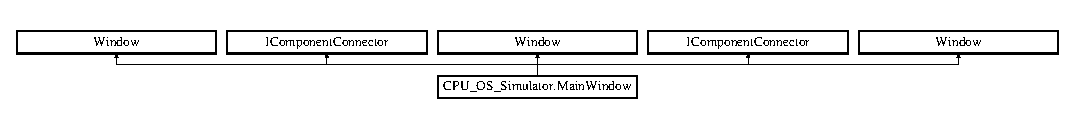
\includegraphics[height=11.000000cm]{class_c_p_u___o_s___simulator_1_1_main_window}
\end{center}
\end{figure}
\subsection*{Public Member Functions}
\begin{DoxyCompactItemize}
\item 
\hyperlink{class_c_p_u___o_s___simulator_1_1_main_window_a33462505a86657583c1560cbf02172bd}{Main\+Window} ()
\begin{DoxyCompactList}\small\item\em Constructor For the main window \end{DoxyCompactList}\item 
\hyperlink{class_c_p_u___o_s___simulator_1_1_c_p_u_1_1_instruction}{Instruction} \hyperlink{class_c_p_u___o_s___simulator_1_1_main_window_aeab49a3421f75049e47ed30b86bf8ad5}{Create\+Instruction} (\hyperlink{namespace_c_p_u___o_s___simulator_1_1_c_p_u_ac29c87bff87ad404c953b2581024043e}{Enum\+Opcodes} opcode, \hyperlink{class_c_p_u___o_s___simulator_1_1_c_p_u_1_1_operand}{Operand} op1, \hyperlink{class_c_p_u___o_s___simulator_1_1_c_p_u_1_1_operand}{Operand} op2, int Size)
\begin{DoxyCompactList}\small\item\em Creates an instruction with 2 operands \end{DoxyCompactList}\item 
\hyperlink{class_c_p_u___o_s___simulator_1_1_c_p_u_1_1_instruction}{Instruction} \hyperlink{class_c_p_u___o_s___simulator_1_1_main_window_a25a43c9a60f98f8196199d04420e48cf}{Create\+Instruction} (\hyperlink{namespace_c_p_u___o_s___simulator_1_1_c_p_u_ac29c87bff87ad404c953b2581024043e}{Enum\+Opcodes} opcode, \hyperlink{class_c_p_u___o_s___simulator_1_1_c_p_u_1_1_operand}{Operand} op1, int Size)
\begin{DoxyCompactList}\small\item\em Creates an instruction with 1 operand \end{DoxyCompactList}\item 
\hyperlink{class_c_p_u___o_s___simulator_1_1_c_p_u_1_1_instruction}{Instruction} \hyperlink{class_c_p_u___o_s___simulator_1_1_main_window_a608bc25c49d397aacde6cdd41d4314c3}{Create\+Instruction} (\hyperlink{namespace_c_p_u___o_s___simulator_1_1_c_p_u_ac29c87bff87ad404c953b2581024043e}{Enum\+Opcodes} opcode, int Size)
\begin{DoxyCompactList}\small\item\em Creates an instruction with no operands \end{DoxyCompactList}\item 
void \hyperlink{class_c_p_u___o_s___simulator_1_1_main_window_ae73f56ccee0f45b0df54438b3d397dd9}{Add\+Instruction} (\hyperlink{class_c_p_u___o_s___simulator_1_1_c_p_u_1_1_instruction}{Instruction} ins, int index)
\begin{DoxyCompactList}\small\item\em Adds an instruction to the currently loaded program \end{DoxyCompactList}\item 
void \hyperlink{class_c_p_u___o_s___simulator_1_1_main_window_a195e7715af146b207e5b973bd10c80c6}{Dispose} ()
\item 
void \hyperlink{class_c_p_u___o_s___simulator_1_1_main_window_a30724af44ae89c2172130c2dd36e145c}{Initialize\+Component} ()
\begin{DoxyCompactList}\small\item\em Initialize\+Component \end{DoxyCompactList}\item 
void \hyperlink{class_c_p_u___o_s___simulator_1_1_main_window_a30724af44ae89c2172130c2dd36e145c}{Initialize\+Component} ()
\begin{DoxyCompactList}\small\item\em Initialize\+Component \end{DoxyCompactList}\item 
void \hyperlink{class_c_p_u___o_s___simulator_1_1_main_window_a30724af44ae89c2172130c2dd36e145c}{Initialize\+Component} ()
\begin{DoxyCompactList}\small\item\em Initialize\+Component \end{DoxyCompactList}\item 
void \hyperlink{class_c_p_u___o_s___simulator_1_1_main_window_a30724af44ae89c2172130c2dd36e145c}{Initialize\+Component} ()
\begin{DoxyCompactList}\small\item\em Initialize\+Component \end{DoxyCompactList}\end{DoxyCompactItemize}
\subsection*{Public Attributes}
\begin{DoxyCompactItemize}
\item 
string \hyperlink{class_c_p_u___o_s___simulator_1_1_main_window_a91f063d9cf776004dc74e719ef942907}{current\+Program} = string.\+Empty
\end{DoxyCompactItemize}
\subsection*{Static Public Attributes}
\begin{DoxyCompactItemize}
\item 
static \hyperlink{class_c_p_u___o_s___simulator_1_1_main_window}{Main\+Window} \hyperlink{class_c_p_u___o_s___simulator_1_1_main_window_a1280266cc57403a91f08a8350dee05cc}{current\+Instance}
\end{DoxyCompactItemize}
\subsection*{Package Attributes}
\begin{DoxyCompactItemize}
\item 
\hyperlink{class_c_p_u___o_s___simulator_1_1_main_window}{C\+P\+U\+\_\+\+O\+S\+\_\+\+Simulator.\+Main\+Window} \hyperlink{class_c_p_u___o_s___simulator_1_1_main_window_adf996cda04d3cf426847b8fd8981ee66}{Main\+Window2}
\item 
System.\+Windows.\+Controls.\+Grid \hyperlink{class_c_p_u___o_s___simulator_1_1_main_window_a5c56d82a7b611446e81b7baa3229d76b}{Main\+Window\+Grid}
\item 
System.\+Windows.\+Controls.\+Grid \hyperlink{class_c_p_u___o_s___simulator_1_1_main_window_a2e6841673af413e8a8f8ba8aa0d7c80b}{Instructions\+Grid}
\item 
System.\+Windows.\+Controls.\+Group\+Box \hyperlink{class_c_p_u___o_s___simulator_1_1_main_window_aebc1256b654d001b7c4ce2bc08522667}{grp\+\_\+\+Instructions\+Box}
\item 
System.\+Windows.\+Controls.\+Grid \hyperlink{class_c_p_u___o_s___simulator_1_1_main_window_a94a99eeb7f5fcfcfbdc375937d5439e7}{Instructions\+Inner\+Grid}
\item 
System.\+Windows.\+Controls.\+List\+View \hyperlink{class_c_p_u___o_s___simulator_1_1_main_window_acdab094f589df9435fa8e3bfe04e61cb}{lst\+\_\+\+Instructions\+List}
\item 
System.\+Windows.\+Controls.\+Primitives.\+Scroll\+Bar \hyperlink{class_c_p_u___o_s___simulator_1_1_main_window_a014812a0e9cd159be05250d94d9a5a8b}{scroll\+Bar1}
\item 
System.\+Windows.\+Controls.\+Grid \hyperlink{class_c_p_u___o_s___simulator_1_1_main_window_ae4f2459995eb2f672c0fd3c2248b79fd}{Operations\+Grid}
\item 
System.\+Windows.\+Controls.\+Tab\+Control \hyperlink{class_c_p_u___o_s___simulator_1_1_main_window_a615ea960969aa9a61afdaef8cf039348}{Program\+Tab}
\item 
System.\+Windows.\+Controls.\+Group\+Box \hyperlink{class_c_p_u___o_s___simulator_1_1_main_window_a1e75e7af485b229372a6aafb84c2ffe0}{grp\+\_\+\+New\+Program}
\item 
System.\+Windows.\+Controls.\+Grid \hyperlink{class_c_p_u___o_s___simulator_1_1_main_window_a38bef5fa03edcca52fa7fc11068923bd}{grid\+\_\+\+New\+Program}
\item 
System.\+Windows.\+Controls.\+Label \hyperlink{class_c_p_u___o_s___simulator_1_1_main_window_ad60038602dcf5d954e420bee89c8494d}{label}
\item 
System.\+Windows.\+Controls.\+Text\+Box \hyperlink{class_c_p_u___o_s___simulator_1_1_main_window_a2c64b45db8c1d7a30c2f9155899cf918}{txt\+Program\+Name}
\item 
System.\+Windows.\+Controls.\+Label \hyperlink{class_c_p_u___o_s___simulator_1_1_main_window_a09b3ba374a620331bc447b32959260c2}{label1}
\item 
System.\+Windows.\+Controls.\+Text\+Box \hyperlink{class_c_p_u___o_s___simulator_1_1_main_window_aa6eeef1bfdd74aa90d6fea68987306ad}{txt\+Base\+Address}
\item 
System.\+Windows.\+Controls.\+Label \hyperlink{class_c_p_u___o_s___simulator_1_1_main_window_a88c7b6748a5e198c673a3c3c5178d3b8}{label2}
\item 
System.\+Windows.\+Controls.\+Combo\+Box \hyperlink{class_c_p_u___o_s___simulator_1_1_main_window_a8da421354f40baef03909c87c3407e3c}{cmb\+\_\+\+Pages}
\item 
System.\+Windows.\+Controls.\+Button \hyperlink{class_c_p_u___o_s___simulator_1_1_main_window_a4f0d9f8f3d56b76616367438d04b4fde}{btn\+\_\+\+Program\+Add}
\item 
System.\+Windows.\+Controls.\+Group\+Box \hyperlink{class_c_p_u___o_s___simulator_1_1_main_window_a2cafe5a8b54ae3e95a770abc594519a0}{grp\+\_\+\+Programs}
\item 
System.\+Windows.\+Controls.\+Grid \hyperlink{class_c_p_u___o_s___simulator_1_1_main_window_a7a4cb93db4cde3b227cbc3155af574d2}{grid\+\_\+\+Programs}
\item 
System.\+Windows.\+Controls.\+Button \hyperlink{class_c_p_u___o_s___simulator_1_1_main_window_a638eee3b21f6ac5d28a5c95c4dad3fc2}{btn\+\_\+\+Save}
\item 
System.\+Windows.\+Controls.\+Button \hyperlink{class_c_p_u___o_s___simulator_1_1_main_window_a29fbdb7afddedc9425472096337ee13b}{btn\+\_\+\+Load}
\item 
System.\+Windows.\+Controls.\+Button \hyperlink{class_c_p_u___o_s___simulator_1_1_main_window_ad56a38e017d6d47d2076b1ec33e3521d}{btn\+\_\+\+Copy\+To\+Clipboard}
\item 
System.\+Windows.\+Controls.\+Label \hyperlink{class_c_p_u___o_s___simulator_1_1_main_window_a9cbfc378965cf635e61c760e11dd5c8a}{lbl\+Program\+List}
\item 
System.\+Windows.\+Controls.\+Combo\+Box \hyperlink{class_c_p_u___o_s___simulator_1_1_main_window_a9871f5933923725d4386a7a7f3f8828f}{cmb\+\_\+\+Program\+List}
\item 
System.\+Windows.\+Controls.\+Label \hyperlink{class_c_p_u___o_s___simulator_1_1_main_window_ae3adff2ef98d792ce094dcc229c293a8}{lbl\+\_\+\+Base\+Address}
\item 
System.\+Windows.\+Controls.\+Text\+Box \hyperlink{class_c_p_u___o_s___simulator_1_1_main_window_ae6c0ce6078d081b2cb99518c68f1cd85}{txt\+Load\+Base\+Address}
\item 
System.\+Windows.\+Controls.\+Check\+Box \hyperlink{class_c_p_u___o_s___simulator_1_1_main_window_a8ade8cf3e5e2ec2374c984dac406b5e9}{chk\+\_\+\+Load\+Base\+Address}
\item 
System.\+Windows.\+Controls.\+Tab\+Item \hyperlink{class_c_p_u___o_s___simulator_1_1_main_window_a4fe9f6d97eb1f2c45b9e5a0363e61557}{Instruction\+Tab}
\item 
System.\+Windows.\+Controls.\+Grid \hyperlink{class_c_p_u___o_s___simulator_1_1_main_window_af09ff1f305e936227c4a975f4c788133}{grid\+\_\+\+Instructions}
\item 
System.\+Windows.\+Controls.\+Button \hyperlink{class_c_p_u___o_s___simulator_1_1_main_window_a50fb8fcd9e592c4987fac4bcb8762785}{btn\+\_\+\+Add\+New}
\item 
System.\+Windows.\+Controls.\+Button \hyperlink{class_c_p_u___o_s___simulator_1_1_main_window_a3c6c4760a8fd64f653fff0ad06374f13}{btn\+\_\+\+Show}
\item 
System.\+Windows.\+Controls.\+Button \hyperlink{class_c_p_u___o_s___simulator_1_1_main_window_ac30720a1b345a3d59312d2d68f742359}{btn\+\_\+\+Undo}
\item 
System.\+Windows.\+Controls.\+Button \hyperlink{class_c_p_u___o_s___simulator_1_1_main_window_a23c681375b103d2294ac79c51f1fb406}{btn\+\_\+\+Insert\+Above}
\item 
System.\+Windows.\+Controls.\+Button \hyperlink{class_c_p_u___o_s___simulator_1_1_main_window_ac6bfabebf21c92a905764305b789df46}{btn\+Move\+Down}
\item 
System.\+Windows.\+Controls.\+Button \hyperlink{class_c_p_u___o_s___simulator_1_1_main_window_ae07013ea273fb1e9f38fd1dd83144371}{btn\+\_\+\+Edit}
\item 
System.\+Windows.\+Controls.\+Button \hyperlink{class_c_p_u___o_s___simulator_1_1_main_window_a7c6c417d0bd3af11e77f86cf2cfb03fe}{btn\+\_\+\+Insert\+Below}
\item 
System.\+Windows.\+Controls.\+Button \hyperlink{class_c_p_u___o_s___simulator_1_1_main_window_aa85d9301fed773f44a352aad64a9d80d}{btn\+Move\+Up}
\item 
System.\+Windows.\+Controls.\+Button \hyperlink{class_c_p_u___o_s___simulator_1_1_main_window_a74623b1e8f8ab1b3b6835bda2e8a9256}{btn\+\_\+\+Delete}
\item 
System.\+Windows.\+Controls.\+Button \hyperlink{class_c_p_u___o_s___simulator_1_1_main_window_a55b2516a7b78d0e79deac7f1a79f3a92}{btn\+\_\+\+Copy}
\item 
System.\+Windows.\+Controls.\+Button \hyperlink{class_c_p_u___o_s___simulator_1_1_main_window_ae2ef9b73d0b5776415c7f3e91c1eaf21}{btn\+Paste\+Above}
\item 
System.\+Windows.\+Controls.\+Button \hyperlink{class_c_p_u___o_s___simulator_1_1_main_window_a1c24521ff648d75bf5991567e1a85b55}{btn\+\_\+\+Paste\+Below}
\item 
System.\+Windows.\+Controls.\+Tab\+Item \hyperlink{class_c_p_u___o_s___simulator_1_1_main_window_a47b1359d9e96abf2b0935eb3392405d4}{Optimize\+Tab}
\item 
System.\+Windows.\+Controls.\+Grid \hyperlink{class_c_p_u___o_s___simulator_1_1_main_window_adb8397cdbc794d18b0379ba7251d2278}{Program\+List\+Grid}
\item 
System.\+Windows.\+Controls.\+Group\+Box \hyperlink{class_c_p_u___o_s___simulator_1_1_main_window_a0ccd227c10c9a0878095ef10c0ff92b7}{grp\+\_\+\+Program\+List}
\item 
System.\+Windows.\+Controls.\+Grid \hyperlink{class_c_p_u___o_s___simulator_1_1_main_window_a4e287cef9f0becaebe0777af8de2d8c9}{Program\+List\+View\+Grid}
\item 
System.\+Windows.\+Controls.\+List\+View \hyperlink{class_c_p_u___o_s___simulator_1_1_main_window_ab33f21e0f19eab104e6f67f44d89daeb}{lst\+\_\+\+Program\+List}
\item 
System.\+Windows.\+Controls.\+Button \hyperlink{class_c_p_u___o_s___simulator_1_1_main_window_af2d1c3293ffaa1d203a9bdb8bf282eab}{btn\+\_\+\+Show\+Memory}
\item 
System.\+Windows.\+Controls.\+Grid \hyperlink{class_c_p_u___o_s___simulator_1_1_main_window_a37acb139db0aa54950350fdb47dfd452}{Register\+Grid}
\item 
System.\+Windows.\+Controls.\+Group\+Box \hyperlink{class_c_p_u___o_s___simulator_1_1_main_window_af858add509dfe2b90f0d356822f73737}{grp\+\_\+\+Registers}
\item 
System.\+Windows.\+Controls.\+Grid \hyperlink{class_c_p_u___o_s___simulator_1_1_main_window_a27d2d9e2ed92e2daa444ca8086a0861e}{Register\+Inner\+Grid}
\item 
System.\+Windows.\+Controls.\+List\+View \hyperlink{class_c_p_u___o_s___simulator_1_1_main_window_ae88013c536662328670f206a4cab99b1}{lst\+\_\+\+Registers}
\item 
System.\+Windows.\+Controls.\+Grid \hyperlink{class_c_p_u___o_s___simulator_1_1_main_window_a7ce98e44f9236ca31eb5bf3ed81c3372}{Special\+Registers\+Grid}
\item 
System.\+Windows.\+Controls.\+Group\+Box \hyperlink{class_c_p_u___o_s___simulator_1_1_main_window_a02e4a81d8689928cb1d459fd3c01bfdf}{grp\+\_\+\+Special\+Registers}
\item 
System.\+Windows.\+Controls.\+Grid \hyperlink{class_c_p_u___o_s___simulator_1_1_main_window_aeef1e97d3e7d589fdab51828260c7b5a}{Special\+Registers\+Inner\+Grid}
\item 
System.\+Windows.\+Controls.\+Label \hyperlink{class_c_p_u___o_s___simulator_1_1_main_window_a94cf4fbdaebb09776745893c2bce1126}{label3}
\item 
System.\+Windows.\+Controls.\+Text\+Box \hyperlink{class_c_p_u___o_s___simulator_1_1_main_window_a7100765f8e26fa4c97a76dd445942b97}{txt\+\_\+\+P\+C}
\item 
System.\+Windows.\+Controls.\+Label \hyperlink{class_c_p_u___o_s___simulator_1_1_main_window_a3473dc873d8c8d8f4bba6e83f5684299}{label4}
\item 
System.\+Windows.\+Controls.\+Text\+Box \hyperlink{class_c_p_u___o_s___simulator_1_1_main_window_a9135c01bacd48e517d7cf46f69ea87d2}{txt\+\_\+\+S\+R}
\item 
System.\+Windows.\+Controls.\+Label \hyperlink{class_c_p_u___o_s___simulator_1_1_main_window_a37b18e7542e985a8984375d0b1cf441e}{label5}
\item 
System.\+Windows.\+Controls.\+Text\+Box \hyperlink{class_c_p_u___o_s___simulator_1_1_main_window_ac2427655774b9ca2b4c368651d5cd9de}{txt\+\_\+\+S\+P}
\item 
System.\+Windows.\+Controls.\+Label \hyperlink{class_c_p_u___o_s___simulator_1_1_main_window_aadfe7782d7e25b730849222805a541f9}{label5\+\_\+\+Copy}
\item 
System.\+Windows.\+Controls.\+Text\+Box \hyperlink{class_c_p_u___o_s___simulator_1_1_main_window_a7a878022ed4cb948598d3685dc821a00}{txt\+\_\+\+B\+R}
\item 
System.\+Windows.\+Controls.\+Group\+Box \hyperlink{class_c_p_u___o_s___simulator_1_1_main_window_a9947d1946c8258ea1fb77d860baa7e0f}{grp\+\_\+\+Status\+Flags}
\item 
System.\+Windows.\+Controls.\+Grid \hyperlink{class_c_p_u___o_s___simulator_1_1_main_window_afdda5e5a39c6e3b99300284ea2640e7c}{Status\+Flags\+Grid}
\item 
System.\+Windows.\+Controls.\+Check\+Box \hyperlink{class_c_p_u___o_s___simulator_1_1_main_window_adfbc519740506214093673b8015ea67d}{chk\+\_\+\+O\+V}
\item 
System.\+Windows.\+Controls.\+Check\+Box \hyperlink{class_c_p_u___o_s___simulator_1_1_main_window_a70c1a75df218201391cf5e0615a600f1}{chk\+\_\+\+Z}
\item 
System.\+Windows.\+Controls.\+Check\+Box \hyperlink{class_c_p_u___o_s___simulator_1_1_main_window_ab8a23e33c5c71e359574de36ccf8d991}{chk\+\_\+\+N}
\item 
System.\+Windows.\+Controls.\+Group\+Box \hyperlink{class_c_p_u___o_s___simulator_1_1_main_window_a0e549bad0f6778b2ea3fffb6c2d1a2bb}{grp\+\_\+\+C\+P\+U\+Mode}
\item 
System.\+Windows.\+Controls.\+Grid \hyperlink{class_c_p_u___o_s___simulator_1_1_main_window_ab6afb45d3f05517e9df6af167752be77}{C\+P\+U\+Mode\+Grid}
\item 
System.\+Windows.\+Controls.\+Radio\+Button \hyperlink{class_c_p_u___o_s___simulator_1_1_main_window_ab9e8d52c337bc24a24d8282dfbf449c8}{rdb\+\_\+\+User}
\item 
System.\+Windows.\+Controls.\+Radio\+Button \hyperlink{class_c_p_u___o_s___simulator_1_1_main_window_a549c6be690b051f4ab15dce643dec656}{rdb\+\_\+\+Kernel}
\item 
System.\+Windows.\+Controls.\+Label \hyperlink{class_c_p_u___o_s___simulator_1_1_main_window_a8f210008776bb163b4c2c2b160aa52be}{label6}
\item 
System.\+Windows.\+Controls.\+Text\+Box \hyperlink{class_c_p_u___o_s___simulator_1_1_main_window_ac6e0cfcdd72688d7bffd100ce6d11a28}{txt\+\_\+\+I\+R}
\item 
System.\+Windows.\+Controls.\+Label \hyperlink{class_c_p_u___o_s___simulator_1_1_main_window_a18612502a8ab2d53d85434e426785022}{label6\+\_\+\+Copy}
\item 
System.\+Windows.\+Controls.\+Text\+Box \hyperlink{class_c_p_u___o_s___simulator_1_1_main_window_a87f8440246e9f6ace0aa4d69b5bba289}{txt\+\_\+\+M\+A\+R}
\item 
System.\+Windows.\+Controls.\+Label \hyperlink{class_c_p_u___o_s___simulator_1_1_main_window_a890bd54d36af19ec881b6a840d6ac8a9}{label6\+\_\+\+Copy1}
\item 
System.\+Windows.\+Controls.\+Text\+Box \hyperlink{class_c_p_u___o_s___simulator_1_1_main_window_a1aa53d1512aa84e476b3649dcda5ced0}{txt\+\_\+\+M\+D\+R}
\item 
System.\+Windows.\+Controls.\+Grid \hyperlink{class_c_p_u___o_s___simulator_1_1_main_window_a59373e8f8822e4efea670d9fb87a1b32}{Program\+Stack\+Grid}
\item 
System.\+Windows.\+Controls.\+Group\+Box \hyperlink{class_c_p_u___o_s___simulator_1_1_main_window_a10687b397ff3a0381a556096a14ed0b0}{grp\+\_\+\+Program\+Stack}
\item 
System.\+Windows.\+Controls.\+Grid \hyperlink{class_c_p_u___o_s___simulator_1_1_main_window_a8c373866c86f6be0e7ef487a5ccb8c3c}{Program\+Stack\+Inner\+Grid}
\item 
System.\+Windows.\+Controls.\+List\+View \hyperlink{class_c_p_u___o_s___simulator_1_1_main_window_a8453db331c7cc1e7c1e711a06b2ec30c}{lst\+\_\+\+Stack}
\item 
System.\+Windows.\+Controls.\+Grid \hyperlink{class_c_p_u___o_s___simulator_1_1_main_window_af6e1d9a71f9501c02b62e8319ba11b5a}{Control\+Unit\+Grid}
\item 
System.\+Windows.\+Controls.\+Tab\+Control \hyperlink{class_c_p_u___o_s___simulator_1_1_main_window_acc893fc507d9ea08cc4a923bdc23091d}{Control\+Tabs}
\item 
System.\+Windows.\+Controls.\+Grid \hyperlink{class_c_p_u___o_s___simulator_1_1_main_window_a0bb4b4233380c349ee3bef69813a684b}{Control\+Unit\+Inner\+Grid}
\item 
System.\+Windows.\+Controls.\+Button \hyperlink{class_c_p_u___o_s___simulator_1_1_main_window_acd572aa9d278af703febb634fc1c34a3}{btn\+\_\+\+Step}
\item 
System.\+Windows.\+Controls.\+Button \hyperlink{class_c_p_u___o_s___simulator_1_1_main_window_ab3286e931d7154605876654bbf092840}{btn\+\_\+\+Run}
\item 
System.\+Windows.\+Controls.\+Button \hyperlink{class_c_p_u___o_s___simulator_1_1_main_window_a1b6b541d9765ca230f537d1d6b6c83aa}{btn\+\_\+\+Stop}
\item 
System.\+Windows.\+Controls.\+Radio\+Button \hyperlink{class_c_p_u___o_s___simulator_1_1_main_window_acba6218f7f716645443533815c6bd7a3}{rdb\+\_\+\+By\+Instruction}
\item 
System.\+Windows.\+Controls.\+Radio\+Button \hyperlink{class_c_p_u___o_s___simulator_1_1_main_window_ab40dcb618f5398ab67213476fe1b86ca}{rdb\+\_\+\+By\+Single\+Tick}
\item 
System.\+Windows.\+Controls.\+Slider \hyperlink{class_c_p_u___o_s___simulator_1_1_main_window_a39cd3af9bb0f8a3ccd06fdd44c9ed6a3}{sld\+\_\+\+Clock\+Speed}
\item 
System.\+Windows.\+Controls.\+Label \hyperlink{class_c_p_u___o_s___simulator_1_1_main_window_a38ed6363fd03954967bda7a099f6b07e}{label7}
\item 
System.\+Windows.\+Controls.\+Label \hyperlink{class_c_p_u___o_s___simulator_1_1_main_window_a216fc6a1692d8a8f8b80b08348c1dcd4}{label8}
\item 
System.\+Windows.\+Controls.\+Button \hyperlink{class_c_p_u___o_s___simulator_1_1_main_window_ada16565fc869dea1d54013009f5892b4}{btn\+\_\+\+Reset\+Program}
\item 
System.\+Windows.\+Controls.\+Button \hyperlink{class_c_p_u___o_s___simulator_1_1_main_window_a967a1b3dbde7ecb1d8091e5eababcc58}{btn\+\_\+\+Show\+P\+C\+B}
\item 
System.\+Windows.\+Controls.\+Grid \hyperlink{class_c_p_u___o_s___simulator_1_1_main_window_a65cbc082cd4737ec0dd8837efa715510}{grid\+\_\+\+Advanced}
\item 
System.\+Windows.\+Controls.\+Tab\+Control \hyperlink{class_c_p_u___o_s___simulator_1_1_main_window_a409f822cf5503ff0a45e14fb0f86a2aa}{advanced\+\_\+\+Tabs}
\item 
System.\+Windows.\+Controls.\+Tab\+Item \hyperlink{class_c_p_u___o_s___simulator_1_1_main_window_aa0cf25219ff7ec68cccc82f780e5f817}{advanced\+\_\+\+Tab}
\item 
System.\+Windows.\+Controls.\+Grid \hyperlink{class_c_p_u___o_s___simulator_1_1_main_window_a50b3891532cc5bfd0cc44e657bf95374}{advanced\+\_\+\+Grid}
\item 
System.\+Windows.\+Controls.\+Button \hyperlink{class_c_p_u___o_s___simulator_1_1_main_window_a9c127982ee67a80b67a9184b3a6e83d3}{btn\+\_\+\+Console}
\end{DoxyCompactItemize}
\subsection*{Properties}
\begin{DoxyCompactItemize}
\item 
List$<$ \hyperlink{class_c_p_u___o_s___simulator_1_1_c_p_u_1_1_simulator_program}{Simulator\+Program} $>$ \hyperlink{class_c_p_u___o_s___simulator_1_1_main_window_a632c91cdd16a7498bbb8dfb3e5df252c}{Program\+List}\hspace{0.3cm}{\ttfamily  \mbox{[}get, set\mbox{]}}
\item 
\hyperlink{namespace_c_p_u___o_s___simulator_adc17a5a5e004084f05dc8e4d3f70e31f}{Enum\+Instruction\+Mode} \hyperlink{class_c_p_u___o_s___simulator_1_1_main_window_a65916937137002c26f9eb1c88cfff519}{Instruction\+Mode}\hspace{0.3cm}{\ttfamily  \mbox{[}get, set\mbox{]}}
\item 
\hyperlink{class_c_p_u___o_s___simulator_1_1_c_p_u_1_1_execution_unit}{Execution\+Unit} \hyperlink{class_c_p_u___o_s___simulator_1_1_main_window_a3d03550a73d7ab18ebd143a38dbf1431}{Active\+Unit}\hspace{0.3cm}{\ttfamily  \mbox{[}get, set\mbox{]}}
\item 
\hyperlink{class_c_p_u___o_s___simulator_1_1_memory_1_1_physical_memory}{Physical\+Memory} \hyperlink{class_c_p_u___o_s___simulator_1_1_main_window_abee63f1a7c5feecf97e7253a65806a5a}{Memory}\hspace{0.3cm}{\ttfamily  \mbox{[}get, set\mbox{]}}
\item 
\hyperlink{class_c_p_u___o_s___simulator_1_1_memory_1_1_swap_space}{Swap\+Space} \hyperlink{class_c_p_u___o_s___simulator_1_1_main_window_a114d0bf1ca63b0d9213537758535aecf}{Swap\+Space}\hspace{0.3cm}{\ttfamily  \mbox{[}get, set\mbox{]}}
\item 
Background\+Worker \hyperlink{class_c_p_u___o_s___simulator_1_1_main_window_aab5d6c95426ebe1e75b7c3bfc0488b84}{Execution\+Worker}\hspace{0.3cm}{\ttfamily  \mbox{[}get, set\mbox{]}}
\end{DoxyCompactItemize}
\subsection*{Private Member Functions}
\begin{DoxyCompactItemize}
\item 
static void \hyperlink{class_c_p_u___o_s___simulator_1_1_main_window_a0bbdb2d3b0e818f2d264770168521059}{S\+H\+Change\+Notify} (uint w\+Event\+Id, uint u\+Flags, Int\+Ptr dw\+Item1, Int\+Ptr dw\+Item2)
\item 
void \hyperlink{class_c_p_u___o_s___simulator_1_1_main_window_a06b2ba04e8c006037cae7b0e40b9c5a0}{Populate\+Registers} ()
\begin{DoxyCompactList}\small\item\em This function populates the register display in the main window \end{DoxyCompactList}\item 
void \hyperlink{class_c_p_u___o_s___simulator_1_1_main_window_a4fbca2d50698a847da4ab82c3f380680}{Update\+Registers} ()
\begin{DoxyCompactList}\small\item\em This function updates the register display in the main window whenever a register value is updated \end{DoxyCompactList}\item 
void \hyperlink{class_c_p_u___o_s___simulator_1_1_main_window_a798838ad3fae6117c8e624047a591931}{Update\+Special\+Registers} ()
\begin{DoxyCompactList}\small\item\em This function updates the values in the U\+I for the special registers \end{DoxyCompactList}\item 
void \hyperlink{class_c_p_u___o_s___simulator_1_1_main_window_a3b945b691332686989cd5b5107f7f98b}{Main\+Window2\+\_\+\+Loaded} (object sender, Routed\+Event\+Args e)
\item 
void \hyperlink{class_c_p_u___o_s___simulator_1_1_main_window_abe3e79941789134ce080390fcafc720e}{btn\+\_\+\+Program\+Add\+\_\+\+Click} (object sender, Routed\+Event\+Args e)
\begin{DoxyCompactList}\small\item\em Creates and adds a program to the program list \end{DoxyCompactList}\item 
\hyperlink{class_c_p_u___o_s___simulator_1_1_c_p_u_1_1_simulator_program}{Simulator\+Program} \hyperlink{class_c_p_u___o_s___simulator_1_1_main_window_a4cb75cfa224757b1dc708b60681ad803}{Create\+New\+Program} ()
\begin{DoxyCompactList}\small\item\em Creates a new program based on entered data \end{DoxyCompactList}\item 
\hyperlink{class_c_p_u___o_s___simulator_1_1_c_p_u_1_1_simulator_program}{Simulator\+Program} \hyperlink{class_c_p_u___o_s___simulator_1_1_main_window_aa735efa9bc97df2ceb545fdce5f351df}{Create\+New\+Program} (string program\+Name, int base\+Address, int pages)
\begin{DoxyCompactList}\small\item\em Creates a new program based on entered data \end{DoxyCompactList}\item 
void \hyperlink{class_c_p_u___o_s___simulator_1_1_main_window_afcb6e2b3719374f56fd8cb1c786bb219}{btn\+\_\+\+Show\+\_\+\+Click} (object sender, Routed\+Event\+Args e)
\begin{DoxyCompactList}\small\item\em Called when the show button is clicked \end{DoxyCompactList}\item 
void \hyperlink{class_c_p_u___o_s___simulator_1_1_main_window_a37c97ac2869b40063089f1af9cd86724}{btn\+\_\+\+Add\+New\+\_\+\+Click} (object sender, Routed\+Event\+Args e)
\begin{DoxyCompactList}\small\item\em Adds a new instruction to the program \end{DoxyCompactList}\item 
void \hyperlink{class_c_p_u___o_s___simulator_1_1_main_window_a8f710b1bee7b3c9360fb5652231b0502}{btn\+\_\+\+Insert\+Above\+\_\+\+Click} (object sender, Routed\+Event\+Args e)
\begin{DoxyCompactList}\small\item\em Adds a new instruction to the program above the selected instruction \end{DoxyCompactList}\item 
void \hyperlink{class_c_p_u___o_s___simulator_1_1_main_window_ac2307db4caedc82b5a6201077fb1c5b7}{btn\+\_\+\+Insert\+Below\+\_\+\+Click} (object sender, Routed\+Event\+Args e)
\begin{DoxyCompactList}\small\item\em Adds a new instruction to the program above below selected instruction \end{DoxyCompactList}\item 
void \hyperlink{class_c_p_u___o_s___simulator_1_1_main_window_a96ea1acde80b84701b58c1d4aaed2b9f}{btn\+\_\+\+Delete\+\_\+\+Click} (object sender, Routed\+Event\+Args e)
\begin{DoxyCompactList}\small\item\em Deletes the selected instruction from the program \end{DoxyCompactList}\item 
void \hyperlink{class_c_p_u___o_s___simulator_1_1_main_window_a622fd6a40ff66a4a87c3d31ccef4313c}{Main\+Window2\+\_\+\+Closing} (object sender, Cancel\+Event\+Args e)
\begin{DoxyCompactList}\small\item\em Called when the window is closing \end{DoxyCompactList}\item 
void \hyperlink{class_c_p_u___o_s___simulator_1_1_main_window_a5013d1984fc170246a5dc0d26c6fc493}{lst\+\_\+\+Instructions\+List\+\_\+\+Selection\+Changed} (object sender, Selection\+Changed\+Event\+Args e)
\item 
void \hyperlink{class_c_p_u___o_s___simulator_1_1_main_window_ab563b461cf3d62bd3c88eeb7921bfa75}{lst\+\_\+\+Program\+List\+\_\+\+Selection\+Changed} (object sender, Selection\+Changed\+Event\+Args e)
\item 
void \hyperlink{class_c_p_u___o_s___simulator_1_1_main_window_abd01bb7788b0c104045bcc93cf03c9d6}{Update\+Stack} ()
\begin{DoxyCompactList}\small\item\em This function updates the stack display in the main window whenever a value is pushed or popped from the stack \end{DoxyCompactList}\item 
void \hyperlink{class_c_p_u___o_s___simulator_1_1_main_window_a677bf9ebdb9fe30caa0f52f93e5390c9}{Update\+Intructions} ()
\begin{DoxyCompactList}\small\item\em Updates the list of instructions \end{DoxyCompactList}\item 
void \hyperlink{class_c_p_u___o_s___simulator_1_1_main_window_a13c54c19f906fc84076fe654f82f5398}{btn\+\_\+\+Load\+\_\+\+Click} (object sender, Routed\+Event\+Args e)
\item 
void \hyperlink{class_c_p_u___o_s___simulator_1_1_main_window_a3bbf0774868d6b5da4ff08d70e236fa6}{btn\+\_\+\+Save\+\_\+\+Click} (object sender, Routed\+Event\+Args e)
\item 
bool \hyperlink{class_c_p_u___o_s___simulator_1_1_main_window_a843bbe93c5c2225820d216cc1cb7d4e9}{Save\+Program} ()
\begin{DoxyCompactList}\small\item\em Saves the program list to a file \end{DoxyCompactList}\item 
bool \hyperlink{class_c_p_u___o_s___simulator_1_1_main_window_ad788d74c9d6582f3302912cbbba410b0}{Load\+Program} ()
\begin{DoxyCompactList}\small\item\em Loads a program list from a file \end{DoxyCompactList}\item 
void \hyperlink{class_c_p_u___o_s___simulator_1_1_main_window_a80985670e45349866a463b766f92e27b}{Serialize\+Object$<$ T $>$} (T serializable\+Object, string file\+Path)
\begin{DoxyCompactList}\small\item\em Serializes a program List. \end{DoxyCompactList}\item 
void \hyperlink{class_c_p_u___o_s___simulator_1_1_main_window_a44e09f35524cd53ddab77488989c5833}{De\+Serialize\+Object$<$ T $>$} (string file\+Name)
\begin{DoxyCompactList}\small\item\em De-\/serializes an .sas file into a program list \end{DoxyCompactList}\item 
void \hyperlink{class_c_p_u___o_s___simulator_1_1_main_window_afe4c815db0eb51ebc480374f5af09d0c}{Bind\+Instruction\+Delegates} (ref \hyperlink{class_c_p_u___o_s___simulator_1_1_c_p_u_1_1_simulator_program}{Simulator\+Program} prog)
\begin{DoxyCompactList}\small\item\em This function rebinds the delegate function to each instruction in a program after it is loaded from a file. \end{DoxyCompactList}\item 
void \hyperlink{class_c_p_u___o_s___simulator_1_1_main_window_ace253c0b4beef8898af97df25666df2f}{sld\+\_\+\+Clock\+Speed\+\_\+\+Value\+Changed} (object sender, Routed\+Property\+Changed\+Event\+Args$<$ double $>$ e)
\item 
void \hyperlink{class_c_p_u___o_s___simulator_1_1_main_window_a897049d123dd2ecf2820b02205ce1969}{btn\+\_\+\+Step\+\_\+\+Click} (object sender, Routed\+Event\+Args e)
\item 
void \hyperlink{class_c_p_u___o_s___simulator_1_1_main_window_a1f4dedca9ad81ea1c92637759515797f}{btn\+\_\+\+Run\+\_\+\+Click} (object sender, Routed\+Event\+Args e)
\item 
void \hyperlink{class_c_p_u___o_s___simulator_1_1_main_window_ad225bd7394d6ad45de9db58b562b91f7}{Create\+Background\+Worker} ()
\begin{DoxyCompactList}\small\item\em Creates a background worker for the execution thread to run on \end{DoxyCompactList}\item 
async void \hyperlink{class_c_p_u___o_s___simulator_1_1_main_window_a27c9bde14aab0b0a82f5e13e0a71c86c}{Update\+Interface} (object sender, Progress\+Changed\+Event\+Args e)
\begin{DoxyCompactList}\small\item\em Asynchronous method called after every instruction is executed to update required values and user interface asynchronously \end{DoxyCompactList}\item 
void \hyperlink{class_c_p_u___o_s___simulator_1_1_main_window_a83ba6352a96515569978030013c84b72}{Create\+Execution\+Thread} (object sender, Do\+Work\+Event\+Args e)
\item 
async Task$<$ int $>$ \hyperlink{class_c_p_u___o_s___simulator_1_1_main_window_adbb759abbf37061f785e82a9e7f7b3e1}{Update\+Interface} ()
\begin{DoxyCompactList}\small\item\em Asynchronous method called after every instruction is executed to update required values and user interface asynchronously \end{DoxyCompactList}\item 
async void \hyperlink{class_c_p_u___o_s___simulator_1_1_main_window_a03d4ec6b5990ad572db709f5305dd7ca}{Execute\+Program} (object program)
\begin{DoxyCompactList}\small\item\em Asynchronous method called to begin executing a program on the execution thread \end{DoxyCompactList}\item 
async Task$<$ int $>$ \hyperlink{class_c_p_u___o_s___simulator_1_1_main_window_a0712c91c3a03a4fabc2cdb2f4ed0a33b}{Call\+From\+Main\+Thread} (Func$<$ Task$<$ int $>$$>$ Function\+Pointer)
\begin{DoxyCompactList}\small\item\em Bridge function used to call functions on the main thread from within the background thread \end{DoxyCompactList}\item 
async Task$<$ string $>$ \hyperlink{class_c_p_u___o_s___simulator_1_1_main_window_ac30c6f157890cb452dc35ec851cc88ad}{Calculate\+Time} (long mills)
\begin{DoxyCompactList}\small\item\em This function calculates the time in seconds the last program took to execute \end{DoxyCompactList}\item 
void \hyperlink{class_c_p_u___o_s___simulator_1_1_main_window_acbdc92abd94c317f978cee0d28af9448}{btn\+\_\+\+Stop\+\_\+\+Click} (object sender, Routed\+Event\+Args e)
\item 
void \hyperlink{class_c_p_u___o_s___simulator_1_1_main_window_a524b638c053cd53f17e44fe225b9dd4f}{btn\+\_\+\+Reset\+Program\+\_\+\+Click} (object sender, Routed\+Event\+Args e)
\item 
void \hyperlink{class_c_p_u___o_s___simulator_1_1_main_window_a19b793a858804e5f7a5611603aeeaf79}{chk\+\_\+\+O\+V\+\_\+\+Checked} (object sender, Routed\+Event\+Args e)
\item 
void \hyperlink{class_c_p_u___o_s___simulator_1_1_main_window_a59f718f48699e2f35c0151057407c38c}{chk\+\_\+\+O\+V\+\_\+\+Unchecked} (object sender, Routed\+Event\+Args e)
\item 
void \hyperlink{class_c_p_u___o_s___simulator_1_1_main_window_ae6186ab1f27e668a1332b7cf72c70f19}{chk\+\_\+\+Z\+\_\+\+Checked} (object sender, Routed\+Event\+Args e)
\item 
void \hyperlink{class_c_p_u___o_s___simulator_1_1_main_window_a21d19250773a14a89aa8285dbe914c22}{chk\+\_\+\+Z\+\_\+\+Unchecked} (object sender, Routed\+Event\+Args e)
\item 
void \hyperlink{class_c_p_u___o_s___simulator_1_1_main_window_a0d0fff66a2f20f19e86f7d8d25aa8915}{chk\+\_\+\+N\+\_\+\+Checked} (object sender, Routed\+Event\+Args e)
\item 
void \hyperlink{class_c_p_u___o_s___simulator_1_1_main_window_afd6ed1a3f1774365c49977ca74daa906}{chk\+\_\+\+N\+\_\+\+Unchecked} (object sender, Routed\+Event\+Args e)
\item 
void \hyperlink{class_c_p_u___o_s___simulator_1_1_main_window_ae0466b84cb9b9aae5c60fe798585b5ed}{btn\+\_\+\+Show\+Memory\+\_\+\+Click} (object sender, Routed\+Event\+Args e)
\item 
void \hyperlink{class_c_p_u___o_s___simulator_1_1_main_window_a48b0283e10f83b8ab7b694ebd0410dd2}{btn\+\_\+\+Console\+\_\+\+Click} (object sender, Routed\+Event\+Args e)
\item 
void System.\+Windows.\+Markup.\+I\+Component\+Connector. \hyperlink{class_c_p_u___o_s___simulator_1_1_main_window_ae66177a5319cf24975b9dfab71bc830e}{Connect} (int connection\+Id, object target)
\item 
void System.\+Windows.\+Markup.\+I\+Component\+Connector. \hyperlink{class_c_p_u___o_s___simulator_1_1_main_window_ae66177a5319cf24975b9dfab71bc830e}{Connect} (int connection\+Id, object target)
\item 
void System.\+Windows.\+Markup.\+I\+Component\+Connector. \hyperlink{class_c_p_u___o_s___simulator_1_1_main_window_ae66177a5319cf24975b9dfab71bc830e}{Connect} (int connection\+Id, object target)
\item 
void System.\+Windows.\+Markup.\+I\+Component\+Connector. \hyperlink{class_c_p_u___o_s___simulator_1_1_main_window_ae66177a5319cf24975b9dfab71bc830e}{Connect} (int connection\+Id, object target)
\end{DoxyCompactItemize}
\subsection*{Static Private Member Functions}
\begin{DoxyCompactItemize}
\item 
static bool \hyperlink{class_c_p_u___o_s___simulator_1_1_main_window_ac84f58171f511e299566cb11c3a53e48}{Is\+Administrator} ()
\item 
static void \hyperlink{class_c_p_u___o_s___simulator_1_1_main_window_ac2d9309ba55c536660c9b98dff7e40b1}{Set\+Association} (string Extension, string Key\+Name, string Open\+With, string File\+Description)
\item 
static string \hyperlink{class_c_p_u___o_s___simulator_1_1_main_window_a4871bf311e6341a2339deff4ad6c2648}{Get\+Program\+Version} ()
\begin{DoxyCompactList}\small\item\em Gets the build number of the running program \end{DoxyCompactList}\end{DoxyCompactItemize}
\subsection*{Private Attributes}
\begin{DoxyCompactItemize}
\item 
List$<$ \hyperlink{class_c_p_u___o_s___simulator_1_1_c_p_u_1_1_simulator_program}{Simulator\+Program} $>$ \hyperlink{class_c_p_u___o_s___simulator_1_1_main_window_a48fa4dc074c098338a652dbd6a3434c7}{program\+List}
\item 
\hyperlink{namespace_c_p_u___o_s___simulator_adc17a5a5e004084f05dc8e4d3f70e31f}{Enum\+Instruction\+Mode} \hyperlink{class_c_p_u___o_s___simulator_1_1_main_window_adcf36837be53f52843bbeb354a16d15c}{instruction\+Mode}
\item 
\hyperlink{class_c_p_u___o_s___simulator_1_1_c_p_u_1_1_execution_unit}{Execution\+Unit} \hyperlink{class_c_p_u___o_s___simulator_1_1_main_window_af00ce05444d9636c688974f706ef397b}{active\+Unit}
\item 
Stopwatch \hyperlink{class_c_p_u___o_s___simulator_1_1_main_window_a880dc01f7c4f093b77ace064d93be1f3}{s}
\item 
Dispatcher \hyperlink{class_c_p_u___o_s___simulator_1_1_main_window_a5115439e688bb7ed25f5237b266e4f3f}{dispatcher} = Dispatcher.\+Current\+Dispatcher
\item 
Background\+Worker \hyperlink{class_c_p_u___o_s___simulator_1_1_main_window_a80e0a87480e4b7f4cfdb47739985b7c7}{execution\+Worker}
\item 
bool \hyperlink{class_c_p_u___o_s___simulator_1_1_main_window_afcd7446d65f9b9370ddf07499c2b8113}{saved} = false
\item 
\hyperlink{class_c_p_u___o_s___simulator_1_1_memory_1_1_page_table_entry}{Page\+Table\+Entry} \hyperlink{class_c_p_u___o_s___simulator_1_1_main_window_a14f6732faabdb632f3d29dbcbbb7059d}{current\+Page}
\item 
\hyperlink{class_c_p_u___o_s___simulator_1_1_memory_1_1_physical_memory}{Physical\+Memory} \hyperlink{class_c_p_u___o_s___simulator_1_1_main_window_a39a29cd60cb4ccbad0415a4e6d6414fa}{memory}
\item 
\hyperlink{class_c_p_u___o_s___simulator_1_1_memory_1_1_swap_space}{Swap\+Space} \hyperlink{class_c_p_u___o_s___simulator_1_1_main_window_ab9638abdc8d65670240a036bc02d813c}{swap\+Space}
\item 
bool \hyperlink{class_c_p_u___o_s___simulator_1_1_main_window_ae8269f86a68d5fdf06180686fc947cc6}{\+\_\+content\+Loaded}
\end{DoxyCompactItemize}


\subsection{Detailed Description}
Interaction logic for Main\+Window.\+xaml 

\hyperlink{class_c_p_u___o_s___simulator_1_1_main_window}{Main\+Window} 

Definition at line 27 of file Main\+Window.\+xaml.\+cs.



\subsection{Constructor \& Destructor Documentation}
\hypertarget{class_c_p_u___o_s___simulator_1_1_main_window_a33462505a86657583c1560cbf02172bd}{}\index{C\+P\+U\+\_\+\+O\+S\+\_\+\+Simulator\+::\+Main\+Window@{C\+P\+U\+\_\+\+O\+S\+\_\+\+Simulator\+::\+Main\+Window}!Main\+Window@{Main\+Window}}
\index{Main\+Window@{Main\+Window}!C\+P\+U\+\_\+\+O\+S\+\_\+\+Simulator\+::\+Main\+Window@{C\+P\+U\+\_\+\+O\+S\+\_\+\+Simulator\+::\+Main\+Window}}
\subsubsection[{Main\+Window()}]{\setlength{\rightskip}{0pt plus 5cm}C\+P\+U\+\_\+\+O\+S\+\_\+\+Simulator.\+Main\+Window.\+Main\+Window (
\begin{DoxyParamCaption}
{}
\end{DoxyParamCaption}
)}\label{class_c_p_u___o_s___simulator_1_1_main_window_a33462505a86657583c1560cbf02172bd}


Constructor For the main window 



Definition at line 113 of file Main\+Window.\+xaml.\+cs.



\subsection{Member Function Documentation}
\hypertarget{class_c_p_u___o_s___simulator_1_1_main_window_ae73f56ccee0f45b0df54438b3d397dd9}{}\index{C\+P\+U\+\_\+\+O\+S\+\_\+\+Simulator\+::\+Main\+Window@{C\+P\+U\+\_\+\+O\+S\+\_\+\+Simulator\+::\+Main\+Window}!Add\+Instruction@{Add\+Instruction}}
\index{Add\+Instruction@{Add\+Instruction}!C\+P\+U\+\_\+\+O\+S\+\_\+\+Simulator\+::\+Main\+Window@{C\+P\+U\+\_\+\+O\+S\+\_\+\+Simulator\+::\+Main\+Window}}
\subsubsection[{Add\+Instruction(\+Instruction ins, int index)}]{\setlength{\rightskip}{0pt plus 5cm}void C\+P\+U\+\_\+\+O\+S\+\_\+\+Simulator.\+Main\+Window.\+Add\+Instruction (
\begin{DoxyParamCaption}
\item[{{\bf Instruction}}]{ins, }
\item[{int}]{index}
\end{DoxyParamCaption}
)}\label{class_c_p_u___o_s___simulator_1_1_main_window_ae73f56ccee0f45b0df54438b3d397dd9}


Adds an instruction to the currently loaded program 


\begin{DoxyParams}{Parameters}
{\em ins} & the instruction to add\\
\hline
{\em index} & the index in the program to add the instruction\\
\hline
\end{DoxyParams}


Definition at line 495 of file Main\+Window.\+xaml.\+cs.

\hypertarget{class_c_p_u___o_s___simulator_1_1_main_window_afe4c815db0eb51ebc480374f5af09d0c}{}\index{C\+P\+U\+\_\+\+O\+S\+\_\+\+Simulator\+::\+Main\+Window@{C\+P\+U\+\_\+\+O\+S\+\_\+\+Simulator\+::\+Main\+Window}!Bind\+Instruction\+Delegates@{Bind\+Instruction\+Delegates}}
\index{Bind\+Instruction\+Delegates@{Bind\+Instruction\+Delegates}!C\+P\+U\+\_\+\+O\+S\+\_\+\+Simulator\+::\+Main\+Window@{C\+P\+U\+\_\+\+O\+S\+\_\+\+Simulator\+::\+Main\+Window}}
\subsubsection[{Bind\+Instruction\+Delegates(ref Simulator\+Program prog)}]{\setlength{\rightskip}{0pt plus 5cm}void C\+P\+U\+\_\+\+O\+S\+\_\+\+Simulator.\+Main\+Window.\+Bind\+Instruction\+Delegates (
\begin{DoxyParamCaption}
\item[{ref {\bf Simulator\+Program}}]{prog}
\end{DoxyParamCaption}
)\hspace{0.3cm}{\ttfamily [private]}}\label{class_c_p_u___o_s___simulator_1_1_main_window_afe4c815db0eb51ebc480374f5af09d0c}


This function rebinds the delegate function to each instruction in a program after it is loaded from a file. 


\begin{DoxyParams}{Parameters}
{\em prog} & the program to bind its instruction delegates \\
\hline
\end{DoxyParams}


Definition at line 764 of file Main\+Window.\+xaml.\+cs.

\hypertarget{class_c_p_u___o_s___simulator_1_1_main_window_a37c97ac2869b40063089f1af9cd86724}{}\index{C\+P\+U\+\_\+\+O\+S\+\_\+\+Simulator\+::\+Main\+Window@{C\+P\+U\+\_\+\+O\+S\+\_\+\+Simulator\+::\+Main\+Window}!btn\+\_\+\+Add\+New\+\_\+\+Click@{btn\+\_\+\+Add\+New\+\_\+\+Click}}
\index{btn\+\_\+\+Add\+New\+\_\+\+Click@{btn\+\_\+\+Add\+New\+\_\+\+Click}!C\+P\+U\+\_\+\+O\+S\+\_\+\+Simulator\+::\+Main\+Window@{C\+P\+U\+\_\+\+O\+S\+\_\+\+Simulator\+::\+Main\+Window}}
\subsubsection[{btn\+\_\+\+Add\+New\+\_\+\+Click(object sender, Routed\+Event\+Args e)}]{\setlength{\rightskip}{0pt plus 5cm}void C\+P\+U\+\_\+\+O\+S\+\_\+\+Simulator.\+Main\+Window.\+btn\+\_\+\+Add\+New\+\_\+\+Click (
\begin{DoxyParamCaption}
\item[{object}]{sender, }
\item[{Routed\+Event\+Args}]{e}
\end{DoxyParamCaption}
)\hspace{0.3cm}{\ttfamily [private]}}\label{class_c_p_u___o_s___simulator_1_1_main_window_a37c97ac2869b40063089f1af9cd86724}


Adds a new instruction to the program 


\begin{DoxyParams}{Parameters}
{\em sender} & \\
\hline
{\em e} & \\
\hline
\end{DoxyParams}


Definition at line 370 of file Main\+Window.\+xaml.\+cs.

\hypertarget{class_c_p_u___o_s___simulator_1_1_main_window_a48b0283e10f83b8ab7b694ebd0410dd2}{}\index{C\+P\+U\+\_\+\+O\+S\+\_\+\+Simulator\+::\+Main\+Window@{C\+P\+U\+\_\+\+O\+S\+\_\+\+Simulator\+::\+Main\+Window}!btn\+\_\+\+Console\+\_\+\+Click@{btn\+\_\+\+Console\+\_\+\+Click}}
\index{btn\+\_\+\+Console\+\_\+\+Click@{btn\+\_\+\+Console\+\_\+\+Click}!C\+P\+U\+\_\+\+O\+S\+\_\+\+Simulator\+::\+Main\+Window@{C\+P\+U\+\_\+\+O\+S\+\_\+\+Simulator\+::\+Main\+Window}}
\subsubsection[{btn\+\_\+\+Console\+\_\+\+Click(object sender, Routed\+Event\+Args e)}]{\setlength{\rightskip}{0pt plus 5cm}void C\+P\+U\+\_\+\+O\+S\+\_\+\+Simulator.\+Main\+Window.\+btn\+\_\+\+Console\+\_\+\+Click (
\begin{DoxyParamCaption}
\item[{object}]{sender, }
\item[{Routed\+Event\+Args}]{e}
\end{DoxyParamCaption}
)\hspace{0.3cm}{\ttfamily [private]}}\label{class_c_p_u___o_s___simulator_1_1_main_window_a48b0283e10f83b8ab7b694ebd0410dd2}


Definition at line 980 of file Main\+Window.\+xaml.\+cs.

\hypertarget{class_c_p_u___o_s___simulator_1_1_main_window_a96ea1acde80b84701b58c1d4aaed2b9f}{}\index{C\+P\+U\+\_\+\+O\+S\+\_\+\+Simulator\+::\+Main\+Window@{C\+P\+U\+\_\+\+O\+S\+\_\+\+Simulator\+::\+Main\+Window}!btn\+\_\+\+Delete\+\_\+\+Click@{btn\+\_\+\+Delete\+\_\+\+Click}}
\index{btn\+\_\+\+Delete\+\_\+\+Click@{btn\+\_\+\+Delete\+\_\+\+Click}!C\+P\+U\+\_\+\+O\+S\+\_\+\+Simulator\+::\+Main\+Window@{C\+P\+U\+\_\+\+O\+S\+\_\+\+Simulator\+::\+Main\+Window}}
\subsubsection[{btn\+\_\+\+Delete\+\_\+\+Click(object sender, Routed\+Event\+Args e)}]{\setlength{\rightskip}{0pt plus 5cm}void C\+P\+U\+\_\+\+O\+S\+\_\+\+Simulator.\+Main\+Window.\+btn\+\_\+\+Delete\+\_\+\+Click (
\begin{DoxyParamCaption}
\item[{object}]{sender, }
\item[{Routed\+Event\+Args}]{e}
\end{DoxyParamCaption}
)\hspace{0.3cm}{\ttfamily [private]}}\label{class_c_p_u___o_s___simulator_1_1_main_window_a96ea1acde80b84701b58c1d4aaed2b9f}


Deletes the selected instruction from the program 


\begin{DoxyParams}{Parameters}
{\em sender} & \\
\hline
{\em e} & \\
\hline
\end{DoxyParams}


Definition at line 406 of file Main\+Window.\+xaml.\+cs.

\hypertarget{class_c_p_u___o_s___simulator_1_1_main_window_a8f710b1bee7b3c9360fb5652231b0502}{}\index{C\+P\+U\+\_\+\+O\+S\+\_\+\+Simulator\+::\+Main\+Window@{C\+P\+U\+\_\+\+O\+S\+\_\+\+Simulator\+::\+Main\+Window}!btn\+\_\+\+Insert\+Above\+\_\+\+Click@{btn\+\_\+\+Insert\+Above\+\_\+\+Click}}
\index{btn\+\_\+\+Insert\+Above\+\_\+\+Click@{btn\+\_\+\+Insert\+Above\+\_\+\+Click}!C\+P\+U\+\_\+\+O\+S\+\_\+\+Simulator\+::\+Main\+Window@{C\+P\+U\+\_\+\+O\+S\+\_\+\+Simulator\+::\+Main\+Window}}
\subsubsection[{btn\+\_\+\+Insert\+Above\+\_\+\+Click(object sender, Routed\+Event\+Args e)}]{\setlength{\rightskip}{0pt plus 5cm}void C\+P\+U\+\_\+\+O\+S\+\_\+\+Simulator.\+Main\+Window.\+btn\+\_\+\+Insert\+Above\+\_\+\+Click (
\begin{DoxyParamCaption}
\item[{object}]{sender, }
\item[{Routed\+Event\+Args}]{e}
\end{DoxyParamCaption}
)\hspace{0.3cm}{\ttfamily [private]}}\label{class_c_p_u___o_s___simulator_1_1_main_window_a8f710b1bee7b3c9360fb5652231b0502}


Adds a new instruction to the program above the selected instruction 


\begin{DoxyParams}{Parameters}
{\em sender} & \\
\hline
{\em e} & \\
\hline
\end{DoxyParams}


Definition at line 382 of file Main\+Window.\+xaml.\+cs.

\hypertarget{class_c_p_u___o_s___simulator_1_1_main_window_ac2307db4caedc82b5a6201077fb1c5b7}{}\index{C\+P\+U\+\_\+\+O\+S\+\_\+\+Simulator\+::\+Main\+Window@{C\+P\+U\+\_\+\+O\+S\+\_\+\+Simulator\+::\+Main\+Window}!btn\+\_\+\+Insert\+Below\+\_\+\+Click@{btn\+\_\+\+Insert\+Below\+\_\+\+Click}}
\index{btn\+\_\+\+Insert\+Below\+\_\+\+Click@{btn\+\_\+\+Insert\+Below\+\_\+\+Click}!C\+P\+U\+\_\+\+O\+S\+\_\+\+Simulator\+::\+Main\+Window@{C\+P\+U\+\_\+\+O\+S\+\_\+\+Simulator\+::\+Main\+Window}}
\subsubsection[{btn\+\_\+\+Insert\+Below\+\_\+\+Click(object sender, Routed\+Event\+Args e)}]{\setlength{\rightskip}{0pt plus 5cm}void C\+P\+U\+\_\+\+O\+S\+\_\+\+Simulator.\+Main\+Window.\+btn\+\_\+\+Insert\+Below\+\_\+\+Click (
\begin{DoxyParamCaption}
\item[{object}]{sender, }
\item[{Routed\+Event\+Args}]{e}
\end{DoxyParamCaption}
)\hspace{0.3cm}{\ttfamily [private]}}\label{class_c_p_u___o_s___simulator_1_1_main_window_ac2307db4caedc82b5a6201077fb1c5b7}


Adds a new instruction to the program above below selected instruction 


\begin{DoxyParams}{Parameters}
{\em sender} & \\
\hline
{\em e} & \\
\hline
\end{DoxyParams}


Definition at line 394 of file Main\+Window.\+xaml.\+cs.

\hypertarget{class_c_p_u___o_s___simulator_1_1_main_window_a13c54c19f906fc84076fe654f82f5398}{}\index{C\+P\+U\+\_\+\+O\+S\+\_\+\+Simulator\+::\+Main\+Window@{C\+P\+U\+\_\+\+O\+S\+\_\+\+Simulator\+::\+Main\+Window}!btn\+\_\+\+Load\+\_\+\+Click@{btn\+\_\+\+Load\+\_\+\+Click}}
\index{btn\+\_\+\+Load\+\_\+\+Click@{btn\+\_\+\+Load\+\_\+\+Click}!C\+P\+U\+\_\+\+O\+S\+\_\+\+Simulator\+::\+Main\+Window@{C\+P\+U\+\_\+\+O\+S\+\_\+\+Simulator\+::\+Main\+Window}}
\subsubsection[{btn\+\_\+\+Load\+\_\+\+Click(object sender, Routed\+Event\+Args e)}]{\setlength{\rightskip}{0pt plus 5cm}void C\+P\+U\+\_\+\+O\+S\+\_\+\+Simulator.\+Main\+Window.\+btn\+\_\+\+Load\+\_\+\+Click (
\begin{DoxyParamCaption}
\item[{object}]{sender, }
\item[{Routed\+Event\+Args}]{e}
\end{DoxyParamCaption}
)\hspace{0.3cm}{\ttfamily [private]}}\label{class_c_p_u___o_s___simulator_1_1_main_window_a13c54c19f906fc84076fe654f82f5398}


Definition at line 639 of file Main\+Window.\+xaml.\+cs.

\hypertarget{class_c_p_u___o_s___simulator_1_1_main_window_abe3e79941789134ce080390fcafc720e}{}\index{C\+P\+U\+\_\+\+O\+S\+\_\+\+Simulator\+::\+Main\+Window@{C\+P\+U\+\_\+\+O\+S\+\_\+\+Simulator\+::\+Main\+Window}!btn\+\_\+\+Program\+Add\+\_\+\+Click@{btn\+\_\+\+Program\+Add\+\_\+\+Click}}
\index{btn\+\_\+\+Program\+Add\+\_\+\+Click@{btn\+\_\+\+Program\+Add\+\_\+\+Click}!C\+P\+U\+\_\+\+O\+S\+\_\+\+Simulator\+::\+Main\+Window@{C\+P\+U\+\_\+\+O\+S\+\_\+\+Simulator\+::\+Main\+Window}}
\subsubsection[{btn\+\_\+\+Program\+Add\+\_\+\+Click(object sender, Routed\+Event\+Args e)}]{\setlength{\rightskip}{0pt plus 5cm}void C\+P\+U\+\_\+\+O\+S\+\_\+\+Simulator.\+Main\+Window.\+btn\+\_\+\+Program\+Add\+\_\+\+Click (
\begin{DoxyParamCaption}
\item[{object}]{sender, }
\item[{Routed\+Event\+Args}]{e}
\end{DoxyParamCaption}
)\hspace{0.3cm}{\ttfamily [private]}}\label{class_c_p_u___o_s___simulator_1_1_main_window_abe3e79941789134ce080390fcafc720e}


Creates and adds a program to the program list 


\begin{DoxyParams}{Parameters}
{\em sender} & the clicked button \\
\hline
{\em e} & the event args\\
\hline
\end{DoxyParams}


Definition at line 310 of file Main\+Window.\+xaml.\+cs.

\hypertarget{class_c_p_u___o_s___simulator_1_1_main_window_a524b638c053cd53f17e44fe225b9dd4f}{}\index{C\+P\+U\+\_\+\+O\+S\+\_\+\+Simulator\+::\+Main\+Window@{C\+P\+U\+\_\+\+O\+S\+\_\+\+Simulator\+::\+Main\+Window}!btn\+\_\+\+Reset\+Program\+\_\+\+Click@{btn\+\_\+\+Reset\+Program\+\_\+\+Click}}
\index{btn\+\_\+\+Reset\+Program\+\_\+\+Click@{btn\+\_\+\+Reset\+Program\+\_\+\+Click}!C\+P\+U\+\_\+\+O\+S\+\_\+\+Simulator\+::\+Main\+Window@{C\+P\+U\+\_\+\+O\+S\+\_\+\+Simulator\+::\+Main\+Window}}
\subsubsection[{btn\+\_\+\+Reset\+Program\+\_\+\+Click(object sender, Routed\+Event\+Args e)}]{\setlength{\rightskip}{0pt plus 5cm}void C\+P\+U\+\_\+\+O\+S\+\_\+\+Simulator.\+Main\+Window.\+btn\+\_\+\+Reset\+Program\+\_\+\+Click (
\begin{DoxyParamCaption}
\item[{object}]{sender, }
\item[{Routed\+Event\+Args}]{e}
\end{DoxyParamCaption}
)\hspace{0.3cm}{\ttfamily [private]}}\label{class_c_p_u___o_s___simulator_1_1_main_window_a524b638c053cd53f17e44fe225b9dd4f}


Definition at line 913 of file Main\+Window.\+xaml.\+cs.

\hypertarget{class_c_p_u___o_s___simulator_1_1_main_window_a1f4dedca9ad81ea1c92637759515797f}{}\index{C\+P\+U\+\_\+\+O\+S\+\_\+\+Simulator\+::\+Main\+Window@{C\+P\+U\+\_\+\+O\+S\+\_\+\+Simulator\+::\+Main\+Window}!btn\+\_\+\+Run\+\_\+\+Click@{btn\+\_\+\+Run\+\_\+\+Click}}
\index{btn\+\_\+\+Run\+\_\+\+Click@{btn\+\_\+\+Run\+\_\+\+Click}!C\+P\+U\+\_\+\+O\+S\+\_\+\+Simulator\+::\+Main\+Window@{C\+P\+U\+\_\+\+O\+S\+\_\+\+Simulator\+::\+Main\+Window}}
\subsubsection[{btn\+\_\+\+Run\+\_\+\+Click(object sender, Routed\+Event\+Args e)}]{\setlength{\rightskip}{0pt plus 5cm}void C\+P\+U\+\_\+\+O\+S\+\_\+\+Simulator.\+Main\+Window.\+btn\+\_\+\+Run\+\_\+\+Click (
\begin{DoxyParamCaption}
\item[{object}]{sender, }
\item[{Routed\+Event\+Args}]{e}
\end{DoxyParamCaption}
)\hspace{0.3cm}{\ttfamily [private]}}\label{class_c_p_u___o_s___simulator_1_1_main_window_a1f4dedca9ad81ea1c92637759515797f}


Definition at line 795 of file Main\+Window.\+xaml.\+cs.

\hypertarget{class_c_p_u___o_s___simulator_1_1_main_window_a3bbf0774868d6b5da4ff08d70e236fa6}{}\index{C\+P\+U\+\_\+\+O\+S\+\_\+\+Simulator\+::\+Main\+Window@{C\+P\+U\+\_\+\+O\+S\+\_\+\+Simulator\+::\+Main\+Window}!btn\+\_\+\+Save\+\_\+\+Click@{btn\+\_\+\+Save\+\_\+\+Click}}
\index{btn\+\_\+\+Save\+\_\+\+Click@{btn\+\_\+\+Save\+\_\+\+Click}!C\+P\+U\+\_\+\+O\+S\+\_\+\+Simulator\+::\+Main\+Window@{C\+P\+U\+\_\+\+O\+S\+\_\+\+Simulator\+::\+Main\+Window}}
\subsubsection[{btn\+\_\+\+Save\+\_\+\+Click(object sender, Routed\+Event\+Args e)}]{\setlength{\rightskip}{0pt plus 5cm}void C\+P\+U\+\_\+\+O\+S\+\_\+\+Simulator.\+Main\+Window.\+btn\+\_\+\+Save\+\_\+\+Click (
\begin{DoxyParamCaption}
\item[{object}]{sender, }
\item[{Routed\+Event\+Args}]{e}
\end{DoxyParamCaption}
)\hspace{0.3cm}{\ttfamily [private]}}\label{class_c_p_u___o_s___simulator_1_1_main_window_a3bbf0774868d6b5da4ff08d70e236fa6}


Definition at line 649 of file Main\+Window.\+xaml.\+cs.

\hypertarget{class_c_p_u___o_s___simulator_1_1_main_window_afcb6e2b3719374f56fd8cb1c786bb219}{}\index{C\+P\+U\+\_\+\+O\+S\+\_\+\+Simulator\+::\+Main\+Window@{C\+P\+U\+\_\+\+O\+S\+\_\+\+Simulator\+::\+Main\+Window}!btn\+\_\+\+Show\+\_\+\+Click@{btn\+\_\+\+Show\+\_\+\+Click}}
\index{btn\+\_\+\+Show\+\_\+\+Click@{btn\+\_\+\+Show\+\_\+\+Click}!C\+P\+U\+\_\+\+O\+S\+\_\+\+Simulator\+::\+Main\+Window@{C\+P\+U\+\_\+\+O\+S\+\_\+\+Simulator\+::\+Main\+Window}}
\subsubsection[{btn\+\_\+\+Show\+\_\+\+Click(object sender, Routed\+Event\+Args e)}]{\setlength{\rightskip}{0pt plus 5cm}void C\+P\+U\+\_\+\+O\+S\+\_\+\+Simulator.\+Main\+Window.\+btn\+\_\+\+Show\+\_\+\+Click (
\begin{DoxyParamCaption}
\item[{object}]{sender, }
\item[{Routed\+Event\+Args}]{e}
\end{DoxyParamCaption}
)\hspace{0.3cm}{\ttfamily [private]}}\label{class_c_p_u___o_s___simulator_1_1_main_window_afcb6e2b3719374f56fd8cb1c786bb219}


Called when the show button is clicked 


\begin{DoxyParams}{Parameters}
{\em sender} & the object that initiated the event\\
\hline
{\em e} & the eventargs\\
\hline
\end{DoxyParams}


Definition at line 358 of file Main\+Window.\+xaml.\+cs.

\hypertarget{class_c_p_u___o_s___simulator_1_1_main_window_ae0466b84cb9b9aae5c60fe798585b5ed}{}\index{C\+P\+U\+\_\+\+O\+S\+\_\+\+Simulator\+::\+Main\+Window@{C\+P\+U\+\_\+\+O\+S\+\_\+\+Simulator\+::\+Main\+Window}!btn\+\_\+\+Show\+Memory\+\_\+\+Click@{btn\+\_\+\+Show\+Memory\+\_\+\+Click}}
\index{btn\+\_\+\+Show\+Memory\+\_\+\+Click@{btn\+\_\+\+Show\+Memory\+\_\+\+Click}!C\+P\+U\+\_\+\+O\+S\+\_\+\+Simulator\+::\+Main\+Window@{C\+P\+U\+\_\+\+O\+S\+\_\+\+Simulator\+::\+Main\+Window}}
\subsubsection[{btn\+\_\+\+Show\+Memory\+\_\+\+Click(object sender, Routed\+Event\+Args e)}]{\setlength{\rightskip}{0pt plus 5cm}void C\+P\+U\+\_\+\+O\+S\+\_\+\+Simulator.\+Main\+Window.\+btn\+\_\+\+Show\+Memory\+\_\+\+Click (
\begin{DoxyParamCaption}
\item[{object}]{sender, }
\item[{Routed\+Event\+Args}]{e}
\end{DoxyParamCaption}
)\hspace{0.3cm}{\ttfamily [private]}}\label{class_c_p_u___o_s___simulator_1_1_main_window_ae0466b84cb9b9aae5c60fe798585b5ed}


Definition at line 972 of file Main\+Window.\+xaml.\+cs.

\hypertarget{class_c_p_u___o_s___simulator_1_1_main_window_a897049d123dd2ecf2820b02205ce1969}{}\index{C\+P\+U\+\_\+\+O\+S\+\_\+\+Simulator\+::\+Main\+Window@{C\+P\+U\+\_\+\+O\+S\+\_\+\+Simulator\+::\+Main\+Window}!btn\+\_\+\+Step\+\_\+\+Click@{btn\+\_\+\+Step\+\_\+\+Click}}
\index{btn\+\_\+\+Step\+\_\+\+Click@{btn\+\_\+\+Step\+\_\+\+Click}!C\+P\+U\+\_\+\+O\+S\+\_\+\+Simulator\+::\+Main\+Window@{C\+P\+U\+\_\+\+O\+S\+\_\+\+Simulator\+::\+Main\+Window}}
\subsubsection[{btn\+\_\+\+Step\+\_\+\+Click(object sender, Routed\+Event\+Args e)}]{\setlength{\rightskip}{0pt plus 5cm}void C\+P\+U\+\_\+\+O\+S\+\_\+\+Simulator.\+Main\+Window.\+btn\+\_\+\+Step\+\_\+\+Click (
\begin{DoxyParamCaption}
\item[{object}]{sender, }
\item[{Routed\+Event\+Args}]{e}
\end{DoxyParamCaption}
)\hspace{0.3cm}{\ttfamily [private]}}\label{class_c_p_u___o_s___simulator_1_1_main_window_a897049d123dd2ecf2820b02205ce1969}


Definition at line 777 of file Main\+Window.\+xaml.\+cs.

\hypertarget{class_c_p_u___o_s___simulator_1_1_main_window_acbdc92abd94c317f978cee0d28af9448}{}\index{C\+P\+U\+\_\+\+O\+S\+\_\+\+Simulator\+::\+Main\+Window@{C\+P\+U\+\_\+\+O\+S\+\_\+\+Simulator\+::\+Main\+Window}!btn\+\_\+\+Stop\+\_\+\+Click@{btn\+\_\+\+Stop\+\_\+\+Click}}
\index{btn\+\_\+\+Stop\+\_\+\+Click@{btn\+\_\+\+Stop\+\_\+\+Click}!C\+P\+U\+\_\+\+O\+S\+\_\+\+Simulator\+::\+Main\+Window@{C\+P\+U\+\_\+\+O\+S\+\_\+\+Simulator\+::\+Main\+Window}}
\subsubsection[{btn\+\_\+\+Stop\+\_\+\+Click(object sender, Routed\+Event\+Args e)}]{\setlength{\rightskip}{0pt plus 5cm}void C\+P\+U\+\_\+\+O\+S\+\_\+\+Simulator.\+Main\+Window.\+btn\+\_\+\+Stop\+\_\+\+Click (
\begin{DoxyParamCaption}
\item[{object}]{sender, }
\item[{Routed\+Event\+Args}]{e}
\end{DoxyParamCaption}
)\hspace{0.3cm}{\ttfamily [private]}}\label{class_c_p_u___o_s___simulator_1_1_main_window_acbdc92abd94c317f978cee0d28af9448}


Definition at line 906 of file Main\+Window.\+xaml.\+cs.

\hypertarget{class_c_p_u___o_s___simulator_1_1_main_window_ac30c6f157890cb452dc35ec851cc88ad}{}\index{C\+P\+U\+\_\+\+O\+S\+\_\+\+Simulator\+::\+Main\+Window@{C\+P\+U\+\_\+\+O\+S\+\_\+\+Simulator\+::\+Main\+Window}!Calculate\+Time@{Calculate\+Time}}
\index{Calculate\+Time@{Calculate\+Time}!C\+P\+U\+\_\+\+O\+S\+\_\+\+Simulator\+::\+Main\+Window@{C\+P\+U\+\_\+\+O\+S\+\_\+\+Simulator\+::\+Main\+Window}}
\subsubsection[{Calculate\+Time(long mills)}]{\setlength{\rightskip}{0pt plus 5cm}async Task$<$string$>$ C\+P\+U\+\_\+\+O\+S\+\_\+\+Simulator.\+Main\+Window.\+Calculate\+Time (
\begin{DoxyParamCaption}
\item[{long}]{mills}
\end{DoxyParamCaption}
)\hspace{0.3cm}{\ttfamily [private]}}\label{class_c_p_u___o_s___simulator_1_1_main_window_ac30c6f157890cb452dc35ec851cc88ad}


This function calculates the time in seconds the last program took to execute 


\begin{DoxyParams}{Parameters}
{\em mills} & the number of milliseconds the last program took to execute\\
\hline
\end{DoxyParams}
\begin{DoxyReturn}{Returns}

\end{DoxyReturn}


Definition at line 897 of file Main\+Window.\+xaml.\+cs.

\hypertarget{class_c_p_u___o_s___simulator_1_1_main_window_a0712c91c3a03a4fabc2cdb2f4ed0a33b}{}\index{C\+P\+U\+\_\+\+O\+S\+\_\+\+Simulator\+::\+Main\+Window@{C\+P\+U\+\_\+\+O\+S\+\_\+\+Simulator\+::\+Main\+Window}!Call\+From\+Main\+Thread@{Call\+From\+Main\+Thread}}
\index{Call\+From\+Main\+Thread@{Call\+From\+Main\+Thread}!C\+P\+U\+\_\+\+O\+S\+\_\+\+Simulator\+::\+Main\+Window@{C\+P\+U\+\_\+\+O\+S\+\_\+\+Simulator\+::\+Main\+Window}}
\subsubsection[{Call\+From\+Main\+Thread(\+Func$<$ Task$<$ int $>$$>$ Function\+Pointer)}]{\setlength{\rightskip}{0pt plus 5cm}async Task$<$int$>$ C\+P\+U\+\_\+\+O\+S\+\_\+\+Simulator.\+Main\+Window.\+Call\+From\+Main\+Thread (
\begin{DoxyParamCaption}
\item[{Func$<$ Task$<$ int $>$$>$}]{Function\+Pointer}
\end{DoxyParamCaption}
)\hspace{0.3cm}{\ttfamily [private]}}\label{class_c_p_u___o_s___simulator_1_1_main_window_a0712c91c3a03a4fabc2cdb2f4ed0a33b}


Bridge function used to call functions on the main thread from within the background thread 


\begin{DoxyParams}{Parameters}
{\em Function\+Pointer} & The function to call \\
\hline
\end{DoxyParams}
\begin{DoxyReturn}{Returns}
A task to indicate to the main thread that the method has finished executing
\end{DoxyReturn}


Definition at line 885 of file Main\+Window.\+xaml.\+cs.

\hypertarget{class_c_p_u___o_s___simulator_1_1_main_window_a0d0fff66a2f20f19e86f7d8d25aa8915}{}\index{C\+P\+U\+\_\+\+O\+S\+\_\+\+Simulator\+::\+Main\+Window@{C\+P\+U\+\_\+\+O\+S\+\_\+\+Simulator\+::\+Main\+Window}!chk\+\_\+\+N\+\_\+\+Checked@{chk\+\_\+\+N\+\_\+\+Checked}}
\index{chk\+\_\+\+N\+\_\+\+Checked@{chk\+\_\+\+N\+\_\+\+Checked}!C\+P\+U\+\_\+\+O\+S\+\_\+\+Simulator\+::\+Main\+Window@{C\+P\+U\+\_\+\+O\+S\+\_\+\+Simulator\+::\+Main\+Window}}
\subsubsection[{chk\+\_\+\+N\+\_\+\+Checked(object sender, Routed\+Event\+Args e)}]{\setlength{\rightskip}{0pt plus 5cm}void C\+P\+U\+\_\+\+O\+S\+\_\+\+Simulator.\+Main\+Window.\+chk\+\_\+\+N\+\_\+\+Checked (
\begin{DoxyParamCaption}
\item[{object}]{sender, }
\item[{Routed\+Event\+Args}]{e}
\end{DoxyParamCaption}
)\hspace{0.3cm}{\ttfamily [private]}}\label{class_c_p_u___o_s___simulator_1_1_main_window_a0d0fff66a2f20f19e86f7d8d25aa8915}


Definition at line 952 of file Main\+Window.\+xaml.\+cs.

\hypertarget{class_c_p_u___o_s___simulator_1_1_main_window_afd6ed1a3f1774365c49977ca74daa906}{}\index{C\+P\+U\+\_\+\+O\+S\+\_\+\+Simulator\+::\+Main\+Window@{C\+P\+U\+\_\+\+O\+S\+\_\+\+Simulator\+::\+Main\+Window}!chk\+\_\+\+N\+\_\+\+Unchecked@{chk\+\_\+\+N\+\_\+\+Unchecked}}
\index{chk\+\_\+\+N\+\_\+\+Unchecked@{chk\+\_\+\+N\+\_\+\+Unchecked}!C\+P\+U\+\_\+\+O\+S\+\_\+\+Simulator\+::\+Main\+Window@{C\+P\+U\+\_\+\+O\+S\+\_\+\+Simulator\+::\+Main\+Window}}
\subsubsection[{chk\+\_\+\+N\+\_\+\+Unchecked(object sender, Routed\+Event\+Args e)}]{\setlength{\rightskip}{0pt plus 5cm}void C\+P\+U\+\_\+\+O\+S\+\_\+\+Simulator.\+Main\+Window.\+chk\+\_\+\+N\+\_\+\+Unchecked (
\begin{DoxyParamCaption}
\item[{object}]{sender, }
\item[{Routed\+Event\+Args}]{e}
\end{DoxyParamCaption}
)\hspace{0.3cm}{\ttfamily [private]}}\label{class_c_p_u___o_s___simulator_1_1_main_window_afd6ed1a3f1774365c49977ca74daa906}


Definition at line 959 of file Main\+Window.\+xaml.\+cs.

\hypertarget{class_c_p_u___o_s___simulator_1_1_main_window_a19b793a858804e5f7a5611603aeeaf79}{}\index{C\+P\+U\+\_\+\+O\+S\+\_\+\+Simulator\+::\+Main\+Window@{C\+P\+U\+\_\+\+O\+S\+\_\+\+Simulator\+::\+Main\+Window}!chk\+\_\+\+O\+V\+\_\+\+Checked@{chk\+\_\+\+O\+V\+\_\+\+Checked}}
\index{chk\+\_\+\+O\+V\+\_\+\+Checked@{chk\+\_\+\+O\+V\+\_\+\+Checked}!C\+P\+U\+\_\+\+O\+S\+\_\+\+Simulator\+::\+Main\+Window@{C\+P\+U\+\_\+\+O\+S\+\_\+\+Simulator\+::\+Main\+Window}}
\subsubsection[{chk\+\_\+\+O\+V\+\_\+\+Checked(object sender, Routed\+Event\+Args e)}]{\setlength{\rightskip}{0pt plus 5cm}void C\+P\+U\+\_\+\+O\+S\+\_\+\+Simulator.\+Main\+Window.\+chk\+\_\+\+O\+V\+\_\+\+Checked (
\begin{DoxyParamCaption}
\item[{object}]{sender, }
\item[{Routed\+Event\+Args}]{e}
\end{DoxyParamCaption}
)\hspace{0.3cm}{\ttfamily [private]}}\label{class_c_p_u___o_s___simulator_1_1_main_window_a19b793a858804e5f7a5611603aeeaf79}


Definition at line 924 of file Main\+Window.\+xaml.\+cs.

\hypertarget{class_c_p_u___o_s___simulator_1_1_main_window_a59f718f48699e2f35c0151057407c38c}{}\index{C\+P\+U\+\_\+\+O\+S\+\_\+\+Simulator\+::\+Main\+Window@{C\+P\+U\+\_\+\+O\+S\+\_\+\+Simulator\+::\+Main\+Window}!chk\+\_\+\+O\+V\+\_\+\+Unchecked@{chk\+\_\+\+O\+V\+\_\+\+Unchecked}}
\index{chk\+\_\+\+O\+V\+\_\+\+Unchecked@{chk\+\_\+\+O\+V\+\_\+\+Unchecked}!C\+P\+U\+\_\+\+O\+S\+\_\+\+Simulator\+::\+Main\+Window@{C\+P\+U\+\_\+\+O\+S\+\_\+\+Simulator\+::\+Main\+Window}}
\subsubsection[{chk\+\_\+\+O\+V\+\_\+\+Unchecked(object sender, Routed\+Event\+Args e)}]{\setlength{\rightskip}{0pt plus 5cm}void C\+P\+U\+\_\+\+O\+S\+\_\+\+Simulator.\+Main\+Window.\+chk\+\_\+\+O\+V\+\_\+\+Unchecked (
\begin{DoxyParamCaption}
\item[{object}]{sender, }
\item[{Routed\+Event\+Args}]{e}
\end{DoxyParamCaption}
)\hspace{0.3cm}{\ttfamily [private]}}\label{class_c_p_u___o_s___simulator_1_1_main_window_a59f718f48699e2f35c0151057407c38c}


Definition at line 931 of file Main\+Window.\+xaml.\+cs.

\hypertarget{class_c_p_u___o_s___simulator_1_1_main_window_ae6186ab1f27e668a1332b7cf72c70f19}{}\index{C\+P\+U\+\_\+\+O\+S\+\_\+\+Simulator\+::\+Main\+Window@{C\+P\+U\+\_\+\+O\+S\+\_\+\+Simulator\+::\+Main\+Window}!chk\+\_\+\+Z\+\_\+\+Checked@{chk\+\_\+\+Z\+\_\+\+Checked}}
\index{chk\+\_\+\+Z\+\_\+\+Checked@{chk\+\_\+\+Z\+\_\+\+Checked}!C\+P\+U\+\_\+\+O\+S\+\_\+\+Simulator\+::\+Main\+Window@{C\+P\+U\+\_\+\+O\+S\+\_\+\+Simulator\+::\+Main\+Window}}
\subsubsection[{chk\+\_\+\+Z\+\_\+\+Checked(object sender, Routed\+Event\+Args e)}]{\setlength{\rightskip}{0pt plus 5cm}void C\+P\+U\+\_\+\+O\+S\+\_\+\+Simulator.\+Main\+Window.\+chk\+\_\+\+Z\+\_\+\+Checked (
\begin{DoxyParamCaption}
\item[{object}]{sender, }
\item[{Routed\+Event\+Args}]{e}
\end{DoxyParamCaption}
)\hspace{0.3cm}{\ttfamily [private]}}\label{class_c_p_u___o_s___simulator_1_1_main_window_ae6186ab1f27e668a1332b7cf72c70f19}


Definition at line 938 of file Main\+Window.\+xaml.\+cs.

\hypertarget{class_c_p_u___o_s___simulator_1_1_main_window_a21d19250773a14a89aa8285dbe914c22}{}\index{C\+P\+U\+\_\+\+O\+S\+\_\+\+Simulator\+::\+Main\+Window@{C\+P\+U\+\_\+\+O\+S\+\_\+\+Simulator\+::\+Main\+Window}!chk\+\_\+\+Z\+\_\+\+Unchecked@{chk\+\_\+\+Z\+\_\+\+Unchecked}}
\index{chk\+\_\+\+Z\+\_\+\+Unchecked@{chk\+\_\+\+Z\+\_\+\+Unchecked}!C\+P\+U\+\_\+\+O\+S\+\_\+\+Simulator\+::\+Main\+Window@{C\+P\+U\+\_\+\+O\+S\+\_\+\+Simulator\+::\+Main\+Window}}
\subsubsection[{chk\+\_\+\+Z\+\_\+\+Unchecked(object sender, Routed\+Event\+Args e)}]{\setlength{\rightskip}{0pt plus 5cm}void C\+P\+U\+\_\+\+O\+S\+\_\+\+Simulator.\+Main\+Window.\+chk\+\_\+\+Z\+\_\+\+Unchecked (
\begin{DoxyParamCaption}
\item[{object}]{sender, }
\item[{Routed\+Event\+Args}]{e}
\end{DoxyParamCaption}
)\hspace{0.3cm}{\ttfamily [private]}}\label{class_c_p_u___o_s___simulator_1_1_main_window_a21d19250773a14a89aa8285dbe914c22}


Definition at line 945 of file Main\+Window.\+xaml.\+cs.

\hypertarget{class_c_p_u___o_s___simulator_1_1_main_window_ae66177a5319cf24975b9dfab71bc830e}{}\index{C\+P\+U\+\_\+\+O\+S\+\_\+\+Simulator\+::\+Main\+Window@{C\+P\+U\+\_\+\+O\+S\+\_\+\+Simulator\+::\+Main\+Window}!Connect@{Connect}}
\index{Connect@{Connect}!C\+P\+U\+\_\+\+O\+S\+\_\+\+Simulator\+::\+Main\+Window@{C\+P\+U\+\_\+\+O\+S\+\_\+\+Simulator\+::\+Main\+Window}}
\subsubsection[{Connect(int connection\+Id, object target)}]{\setlength{\rightskip}{0pt plus 5cm}void System.\+Windows.\+Markup.\+I\+Component\+Connector. C\+P\+U\+\_\+\+O\+S\+\_\+\+Simulator.\+Main\+Window.\+Connect (
\begin{DoxyParamCaption}
\item[{int}]{connection\+Id, }
\item[{object}]{target}
\end{DoxyParamCaption}
)\hspace{0.3cm}{\ttfamily [private]}}\label{class_c_p_u___o_s___simulator_1_1_main_window_ae66177a5319cf24975b9dfab71bc830e}


Definition at line 830 of file Main\+Window.\+g.\+cs.

\hypertarget{class_c_p_u___o_s___simulator_1_1_main_window_ae66177a5319cf24975b9dfab71bc830e}{}\index{C\+P\+U\+\_\+\+O\+S\+\_\+\+Simulator\+::\+Main\+Window@{C\+P\+U\+\_\+\+O\+S\+\_\+\+Simulator\+::\+Main\+Window}!Connect@{Connect}}
\index{Connect@{Connect}!C\+P\+U\+\_\+\+O\+S\+\_\+\+Simulator\+::\+Main\+Window@{C\+P\+U\+\_\+\+O\+S\+\_\+\+Simulator\+::\+Main\+Window}}
\subsubsection[{Connect(int connection\+Id, object target)}]{\setlength{\rightskip}{0pt plus 5cm}void System.\+Windows.\+Markup.\+I\+Component\+Connector. C\+P\+U\+\_\+\+O\+S\+\_\+\+Simulator.\+Main\+Window.\+Connect (
\begin{DoxyParamCaption}
\item[{int}]{connection\+Id, }
\item[{object}]{target}
\end{DoxyParamCaption}
)\hspace{0.3cm}{\ttfamily [private]}}\label{class_c_p_u___o_s___simulator_1_1_main_window_ae66177a5319cf24975b9dfab71bc830e}


Definition at line 830 of file Main\+Window.\+g.\+i.\+cs.

\hypertarget{class_c_p_u___o_s___simulator_1_1_main_window_ae66177a5319cf24975b9dfab71bc830e}{}\index{C\+P\+U\+\_\+\+O\+S\+\_\+\+Simulator\+::\+Main\+Window@{C\+P\+U\+\_\+\+O\+S\+\_\+\+Simulator\+::\+Main\+Window}!Connect@{Connect}}
\index{Connect@{Connect}!C\+P\+U\+\_\+\+O\+S\+\_\+\+Simulator\+::\+Main\+Window@{C\+P\+U\+\_\+\+O\+S\+\_\+\+Simulator\+::\+Main\+Window}}
\subsubsection[{Connect(int connection\+Id, object target)}]{\setlength{\rightskip}{0pt plus 5cm}void System.\+Windows.\+Markup.\+I\+Component\+Connector. C\+P\+U\+\_\+\+O\+S\+\_\+\+Simulator.\+Main\+Window.\+Connect (
\begin{DoxyParamCaption}
\item[{int}]{connection\+Id, }
\item[{object}]{target}
\end{DoxyParamCaption}
)\hspace{0.3cm}{\ttfamily [private]}}\label{class_c_p_u___o_s___simulator_1_1_main_window_ae66177a5319cf24975b9dfab71bc830e}


Definition at line 870 of file Main\+Window.\+g.\+cs.

\hypertarget{class_c_p_u___o_s___simulator_1_1_main_window_ae66177a5319cf24975b9dfab71bc830e}{}\index{C\+P\+U\+\_\+\+O\+S\+\_\+\+Simulator\+::\+Main\+Window@{C\+P\+U\+\_\+\+O\+S\+\_\+\+Simulator\+::\+Main\+Window}!Connect@{Connect}}
\index{Connect@{Connect}!C\+P\+U\+\_\+\+O\+S\+\_\+\+Simulator\+::\+Main\+Window@{C\+P\+U\+\_\+\+O\+S\+\_\+\+Simulator\+::\+Main\+Window}}
\subsubsection[{Connect(int connection\+Id, object target)}]{\setlength{\rightskip}{0pt plus 5cm}void System.\+Windows.\+Markup.\+I\+Component\+Connector. C\+P\+U\+\_\+\+O\+S\+\_\+\+Simulator.\+Main\+Window.\+Connect (
\begin{DoxyParamCaption}
\item[{int}]{connection\+Id, }
\item[{object}]{target}
\end{DoxyParamCaption}
)\hspace{0.3cm}{\ttfamily [private]}}\label{class_c_p_u___o_s___simulator_1_1_main_window_ae66177a5319cf24975b9dfab71bc830e}


Definition at line 870 of file Main\+Window.\+g.\+i.\+cs.

\hypertarget{class_c_p_u___o_s___simulator_1_1_main_window_ad225bd7394d6ad45de9db58b562b91f7}{}\index{C\+P\+U\+\_\+\+O\+S\+\_\+\+Simulator\+::\+Main\+Window@{C\+P\+U\+\_\+\+O\+S\+\_\+\+Simulator\+::\+Main\+Window}!Create\+Background\+Worker@{Create\+Background\+Worker}}
\index{Create\+Background\+Worker@{Create\+Background\+Worker}!C\+P\+U\+\_\+\+O\+S\+\_\+\+Simulator\+::\+Main\+Window@{C\+P\+U\+\_\+\+O\+S\+\_\+\+Simulator\+::\+Main\+Window}}
\subsubsection[{Create\+Background\+Worker()}]{\setlength{\rightskip}{0pt plus 5cm}void C\+P\+U\+\_\+\+O\+S\+\_\+\+Simulator.\+Main\+Window.\+Create\+Background\+Worker (
\begin{DoxyParamCaption}
{}
\end{DoxyParamCaption}
)\hspace{0.3cm}{\ttfamily [private]}}\label{class_c_p_u___o_s___simulator_1_1_main_window_ad225bd7394d6ad45de9db58b562b91f7}


Creates a background worker for the execution thread to run on 



Definition at line 811 of file Main\+Window.\+xaml.\+cs.

\hypertarget{class_c_p_u___o_s___simulator_1_1_main_window_a83ba6352a96515569978030013c84b72}{}\index{C\+P\+U\+\_\+\+O\+S\+\_\+\+Simulator\+::\+Main\+Window@{C\+P\+U\+\_\+\+O\+S\+\_\+\+Simulator\+::\+Main\+Window}!Create\+Execution\+Thread@{Create\+Execution\+Thread}}
\index{Create\+Execution\+Thread@{Create\+Execution\+Thread}!C\+P\+U\+\_\+\+O\+S\+\_\+\+Simulator\+::\+Main\+Window@{C\+P\+U\+\_\+\+O\+S\+\_\+\+Simulator\+::\+Main\+Window}}
\subsubsection[{Create\+Execution\+Thread(object sender, Do\+Work\+Event\+Args e)}]{\setlength{\rightskip}{0pt plus 5cm}void C\+P\+U\+\_\+\+O\+S\+\_\+\+Simulator.\+Main\+Window.\+Create\+Execution\+Thread (
\begin{DoxyParamCaption}
\item[{object}]{sender, }
\item[{Do\+Work\+Event\+Args}]{e}
\end{DoxyParamCaption}
)\hspace{0.3cm}{\ttfamily [private]}}\label{class_c_p_u___o_s___simulator_1_1_main_window_a83ba6352a96515569978030013c84b72}


Definition at line 838 of file Main\+Window.\+xaml.\+cs.

\hypertarget{class_c_p_u___o_s___simulator_1_1_main_window_aeab49a3421f75049e47ed30b86bf8ad5}{}\index{C\+P\+U\+\_\+\+O\+S\+\_\+\+Simulator\+::\+Main\+Window@{C\+P\+U\+\_\+\+O\+S\+\_\+\+Simulator\+::\+Main\+Window}!Create\+Instruction@{Create\+Instruction}}
\index{Create\+Instruction@{Create\+Instruction}!C\+P\+U\+\_\+\+O\+S\+\_\+\+Simulator\+::\+Main\+Window@{C\+P\+U\+\_\+\+O\+S\+\_\+\+Simulator\+::\+Main\+Window}}
\subsubsection[{Create\+Instruction(\+Enum\+Opcodes opcode, Operand op1, Operand op2, int Size)}]{\setlength{\rightskip}{0pt plus 5cm}{\bf Instruction} C\+P\+U\+\_\+\+O\+S\+\_\+\+Simulator.\+Main\+Window.\+Create\+Instruction (
\begin{DoxyParamCaption}
\item[{{\bf Enum\+Opcodes}}]{opcode, }
\item[{{\bf Operand}}]{op1, }
\item[{{\bf Operand}}]{op2, }
\item[{int}]{Size}
\end{DoxyParamCaption}
)}\label{class_c_p_u___o_s___simulator_1_1_main_window_aeab49a3421f75049e47ed30b86bf8ad5}


Creates an instruction with 2 operands 


\begin{DoxyParams}{Parameters}
{\em opcode} & the instruction opcode\\
\hline
{\em op1} & the first operand\\
\hline
{\em op2} & the second operand\\
\hline
{\em Size} & the size of the instruction\\
\hline
\end{DoxyParams}
\begin{DoxyReturn}{Returns}

\end{DoxyReturn}


Definition at line 464 of file Main\+Window.\+xaml.\+cs.

\hypertarget{class_c_p_u___o_s___simulator_1_1_main_window_a25a43c9a60f98f8196199d04420e48cf}{}\index{C\+P\+U\+\_\+\+O\+S\+\_\+\+Simulator\+::\+Main\+Window@{C\+P\+U\+\_\+\+O\+S\+\_\+\+Simulator\+::\+Main\+Window}!Create\+Instruction@{Create\+Instruction}}
\index{Create\+Instruction@{Create\+Instruction}!C\+P\+U\+\_\+\+O\+S\+\_\+\+Simulator\+::\+Main\+Window@{C\+P\+U\+\_\+\+O\+S\+\_\+\+Simulator\+::\+Main\+Window}}
\subsubsection[{Create\+Instruction(\+Enum\+Opcodes opcode, Operand op1, int Size)}]{\setlength{\rightskip}{0pt plus 5cm}{\bf Instruction} C\+P\+U\+\_\+\+O\+S\+\_\+\+Simulator.\+Main\+Window.\+Create\+Instruction (
\begin{DoxyParamCaption}
\item[{{\bf Enum\+Opcodes}}]{opcode, }
\item[{{\bf Operand}}]{op1, }
\item[{int}]{Size}
\end{DoxyParamCaption}
)}\label{class_c_p_u___o_s___simulator_1_1_main_window_a25a43c9a60f98f8196199d04420e48cf}


Creates an instruction with 1 operand 


\begin{DoxyParams}{Parameters}
{\em opcode} & the instruction opcode\\
\hline
{\em op1} & the first operand\\
\hline
{\em Size} & the size of the instruction\\
\hline
\end{DoxyParams}


Definition at line 475 of file Main\+Window.\+xaml.\+cs.

\hypertarget{class_c_p_u___o_s___simulator_1_1_main_window_a608bc25c49d397aacde6cdd41d4314c3}{}\index{C\+P\+U\+\_\+\+O\+S\+\_\+\+Simulator\+::\+Main\+Window@{C\+P\+U\+\_\+\+O\+S\+\_\+\+Simulator\+::\+Main\+Window}!Create\+Instruction@{Create\+Instruction}}
\index{Create\+Instruction@{Create\+Instruction}!C\+P\+U\+\_\+\+O\+S\+\_\+\+Simulator\+::\+Main\+Window@{C\+P\+U\+\_\+\+O\+S\+\_\+\+Simulator\+::\+Main\+Window}}
\subsubsection[{Create\+Instruction(\+Enum\+Opcodes opcode, int Size)}]{\setlength{\rightskip}{0pt plus 5cm}{\bf Instruction} C\+P\+U\+\_\+\+O\+S\+\_\+\+Simulator.\+Main\+Window.\+Create\+Instruction (
\begin{DoxyParamCaption}
\item[{{\bf Enum\+Opcodes}}]{opcode, }
\item[{int}]{Size}
\end{DoxyParamCaption}
)}\label{class_c_p_u___o_s___simulator_1_1_main_window_a608bc25c49d397aacde6cdd41d4314c3}


Creates an instruction with no operands 


\begin{DoxyParams}{Parameters}
{\em opcode} & the instruction opcode\\
\hline
{\em Size} & the size of the instruction\\
\hline
\end{DoxyParams}


Definition at line 485 of file Main\+Window.\+xaml.\+cs.

\hypertarget{class_c_p_u___o_s___simulator_1_1_main_window_a4cb75cfa224757b1dc708b60681ad803}{}\index{C\+P\+U\+\_\+\+O\+S\+\_\+\+Simulator\+::\+Main\+Window@{C\+P\+U\+\_\+\+O\+S\+\_\+\+Simulator\+::\+Main\+Window}!Create\+New\+Program@{Create\+New\+Program}}
\index{Create\+New\+Program@{Create\+New\+Program}!C\+P\+U\+\_\+\+O\+S\+\_\+\+Simulator\+::\+Main\+Window@{C\+P\+U\+\_\+\+O\+S\+\_\+\+Simulator\+::\+Main\+Window}}
\subsubsection[{Create\+New\+Program()}]{\setlength{\rightskip}{0pt plus 5cm}{\bf Simulator\+Program} C\+P\+U\+\_\+\+O\+S\+\_\+\+Simulator.\+Main\+Window.\+Create\+New\+Program (
\begin{DoxyParamCaption}
{}
\end{DoxyParamCaption}
)\hspace{0.3cm}{\ttfamily [private]}}\label{class_c_p_u___o_s___simulator_1_1_main_window_a4cb75cfa224757b1dc708b60681ad803}


Creates a new program based on entered data 

\begin{DoxyReturn}{Returns}
the created program
\end{DoxyReturn}


Definition at line 323 of file Main\+Window.\+xaml.\+cs.

\hypertarget{class_c_p_u___o_s___simulator_1_1_main_window_aa735efa9bc97df2ceb545fdce5f351df}{}\index{C\+P\+U\+\_\+\+O\+S\+\_\+\+Simulator\+::\+Main\+Window@{C\+P\+U\+\_\+\+O\+S\+\_\+\+Simulator\+::\+Main\+Window}!Create\+New\+Program@{Create\+New\+Program}}
\index{Create\+New\+Program@{Create\+New\+Program}!C\+P\+U\+\_\+\+O\+S\+\_\+\+Simulator\+::\+Main\+Window@{C\+P\+U\+\_\+\+O\+S\+\_\+\+Simulator\+::\+Main\+Window}}
\subsubsection[{Create\+New\+Program(string program\+Name, int base\+Address, int pages)}]{\setlength{\rightskip}{0pt plus 5cm}{\bf Simulator\+Program} C\+P\+U\+\_\+\+O\+S\+\_\+\+Simulator.\+Main\+Window.\+Create\+New\+Program (
\begin{DoxyParamCaption}
\item[{string}]{program\+Name, }
\item[{int}]{base\+Address, }
\item[{int}]{pages}
\end{DoxyParamCaption}
)\hspace{0.3cm}{\ttfamily [private]}}\label{class_c_p_u___o_s___simulator_1_1_main_window_aa735efa9bc97df2ceb545fdce5f351df}


Creates a new program based on entered data 

\begin{DoxyReturn}{Returns}
the created program
\end{DoxyReturn}


Definition at line 347 of file Main\+Window.\+xaml.\+cs.

\hypertarget{class_c_p_u___o_s___simulator_1_1_main_window_a44e09f35524cd53ddab77488989c5833}{}\index{C\+P\+U\+\_\+\+O\+S\+\_\+\+Simulator\+::\+Main\+Window@{C\+P\+U\+\_\+\+O\+S\+\_\+\+Simulator\+::\+Main\+Window}!De\+Serialize\+Object$<$ T $>$@{De\+Serialize\+Object$<$ T $>$}}
\index{De\+Serialize\+Object$<$ T $>$@{De\+Serialize\+Object$<$ T $>$}!C\+P\+U\+\_\+\+O\+S\+\_\+\+Simulator\+::\+Main\+Window@{C\+P\+U\+\_\+\+O\+S\+\_\+\+Simulator\+::\+Main\+Window}}
\subsubsection[{De\+Serialize\+Object$<$ T $>$(string file\+Name)}]{\setlength{\rightskip}{0pt plus 5cm}void C\+P\+U\+\_\+\+O\+S\+\_\+\+Simulator.\+Main\+Window.\+De\+Serialize\+Object$<$ T $>$ (
\begin{DoxyParamCaption}
\item[{string}]{file\+Name}
\end{DoxyParamCaption}
)\hspace{0.3cm}{\ttfamily [private]}}\label{class_c_p_u___o_s___simulator_1_1_main_window_a44e09f35524cd53ddab77488989c5833}


De-\/serializes an .sas file into a program list 


\begin{DoxyTemplParams}{Template Parameters}
{\em T} & The type to deserialise\\
\hline
\end{DoxyTemplParams}

\begin{DoxyParams}{Parameters}
{\em file\+Name} & the name of the file to load the objects from\\
\hline
\end{DoxyParams}


Definition at line 728 of file Main\+Window.\+xaml.\+cs.

\hypertarget{class_c_p_u___o_s___simulator_1_1_main_window_a195e7715af146b207e5b973bd10c80c6}{}\index{C\+P\+U\+\_\+\+O\+S\+\_\+\+Simulator\+::\+Main\+Window@{C\+P\+U\+\_\+\+O\+S\+\_\+\+Simulator\+::\+Main\+Window}!Dispose@{Dispose}}
\index{Dispose@{Dispose}!C\+P\+U\+\_\+\+O\+S\+\_\+\+Simulator\+::\+Main\+Window@{C\+P\+U\+\_\+\+O\+S\+\_\+\+Simulator\+::\+Main\+Window}}
\subsubsection[{Dispose()}]{\setlength{\rightskip}{0pt plus 5cm}void C\+P\+U\+\_\+\+O\+S\+\_\+\+Simulator.\+Main\+Window.\+Dispose (
\begin{DoxyParamCaption}
{}
\end{DoxyParamCaption}
)}\label{class_c_p_u___o_s___simulator_1_1_main_window_a195e7715af146b207e5b973bd10c80c6}


Definition at line 966 of file Main\+Window.\+xaml.\+cs.

\hypertarget{class_c_p_u___o_s___simulator_1_1_main_window_a03d4ec6b5990ad572db709f5305dd7ca}{}\index{C\+P\+U\+\_\+\+O\+S\+\_\+\+Simulator\+::\+Main\+Window@{C\+P\+U\+\_\+\+O\+S\+\_\+\+Simulator\+::\+Main\+Window}!Execute\+Program@{Execute\+Program}}
\index{Execute\+Program@{Execute\+Program}!C\+P\+U\+\_\+\+O\+S\+\_\+\+Simulator\+::\+Main\+Window@{C\+P\+U\+\_\+\+O\+S\+\_\+\+Simulator\+::\+Main\+Window}}
\subsubsection[{Execute\+Program(object program)}]{\setlength{\rightskip}{0pt plus 5cm}async void C\+P\+U\+\_\+\+O\+S\+\_\+\+Simulator.\+Main\+Window.\+Execute\+Program (
\begin{DoxyParamCaption}
\item[{object}]{program}
\end{DoxyParamCaption}
)\hspace{0.3cm}{\ttfamily [private]}}\label{class_c_p_u___o_s___simulator_1_1_main_window_a03d4ec6b5990ad572db709f5305dd7ca}


Asynchronous method called to begin executing a program on the execution thread 


\begin{DoxyParams}{Parameters}
{\em program} & The program object to execute\\
\hline
\end{DoxyParams}


Definition at line 867 of file Main\+Window.\+xaml.\+cs.

\hypertarget{class_c_p_u___o_s___simulator_1_1_main_window_a4871bf311e6341a2339deff4ad6c2648}{}\index{C\+P\+U\+\_\+\+O\+S\+\_\+\+Simulator\+::\+Main\+Window@{C\+P\+U\+\_\+\+O\+S\+\_\+\+Simulator\+::\+Main\+Window}!Get\+Program\+Version@{Get\+Program\+Version}}
\index{Get\+Program\+Version@{Get\+Program\+Version}!C\+P\+U\+\_\+\+O\+S\+\_\+\+Simulator\+::\+Main\+Window@{C\+P\+U\+\_\+\+O\+S\+\_\+\+Simulator\+::\+Main\+Window}}
\subsubsection[{Get\+Program\+Version()}]{\setlength{\rightskip}{0pt plus 5cm}static string C\+P\+U\+\_\+\+O\+S\+\_\+\+Simulator.\+Main\+Window.\+Get\+Program\+Version (
\begin{DoxyParamCaption}
{}
\end{DoxyParamCaption}
)\hspace{0.3cm}{\ttfamily [static]}, {\ttfamily [private]}}\label{class_c_p_u___o_s___simulator_1_1_main_window_a4871bf311e6341a2339deff4ad6c2648}


Gets the build number of the running program 

\begin{DoxyReturn}{Returns}
The build number of the running program
\end{DoxyReturn}


Definition at line 298 of file Main\+Window.\+xaml.\+cs.

\hypertarget{class_c_p_u___o_s___simulator_1_1_main_window_a30724af44ae89c2172130c2dd36e145c}{}\index{C\+P\+U\+\_\+\+O\+S\+\_\+\+Simulator\+::\+Main\+Window@{C\+P\+U\+\_\+\+O\+S\+\_\+\+Simulator\+::\+Main\+Window}!Initialize\+Component@{Initialize\+Component}}
\index{Initialize\+Component@{Initialize\+Component}!C\+P\+U\+\_\+\+O\+S\+\_\+\+Simulator\+::\+Main\+Window@{C\+P\+U\+\_\+\+O\+S\+\_\+\+Simulator\+::\+Main\+Window}}
\subsubsection[{Initialize\+Component()}]{\setlength{\rightskip}{0pt plus 5cm}void C\+P\+U\+\_\+\+O\+S\+\_\+\+Simulator.\+Main\+Window.\+Initialize\+Component (
\begin{DoxyParamCaption}
{}
\end{DoxyParamCaption}
)}\label{class_c_p_u___o_s___simulator_1_1_main_window_a30724af44ae89c2172130c2dd36e145c}


Initialize\+Component 



Definition at line 810 of file Main\+Window.\+g.\+i.\+cs.

\hypertarget{class_c_p_u___o_s___simulator_1_1_main_window_a30724af44ae89c2172130c2dd36e145c}{}\index{C\+P\+U\+\_\+\+O\+S\+\_\+\+Simulator\+::\+Main\+Window@{C\+P\+U\+\_\+\+O\+S\+\_\+\+Simulator\+::\+Main\+Window}!Initialize\+Component@{Initialize\+Component}}
\index{Initialize\+Component@{Initialize\+Component}!C\+P\+U\+\_\+\+O\+S\+\_\+\+Simulator\+::\+Main\+Window@{C\+P\+U\+\_\+\+O\+S\+\_\+\+Simulator\+::\+Main\+Window}}
\subsubsection[{Initialize\+Component()}]{\setlength{\rightskip}{0pt plus 5cm}void C\+P\+U\+\_\+\+O\+S\+\_\+\+Simulator.\+Main\+Window.\+Initialize\+Component (
\begin{DoxyParamCaption}
{}
\end{DoxyParamCaption}
)}\label{class_c_p_u___o_s___simulator_1_1_main_window_a30724af44ae89c2172130c2dd36e145c}


Initialize\+Component 



Definition at line 810 of file Main\+Window.\+g.\+cs.

\hypertarget{class_c_p_u___o_s___simulator_1_1_main_window_a30724af44ae89c2172130c2dd36e145c}{}\index{C\+P\+U\+\_\+\+O\+S\+\_\+\+Simulator\+::\+Main\+Window@{C\+P\+U\+\_\+\+O\+S\+\_\+\+Simulator\+::\+Main\+Window}!Initialize\+Component@{Initialize\+Component}}
\index{Initialize\+Component@{Initialize\+Component}!C\+P\+U\+\_\+\+O\+S\+\_\+\+Simulator\+::\+Main\+Window@{C\+P\+U\+\_\+\+O\+S\+\_\+\+Simulator\+::\+Main\+Window}}
\subsubsection[{Initialize\+Component()}]{\setlength{\rightskip}{0pt plus 5cm}void C\+P\+U\+\_\+\+O\+S\+\_\+\+Simulator.\+Main\+Window.\+Initialize\+Component (
\begin{DoxyParamCaption}
{}
\end{DoxyParamCaption}
)}\label{class_c_p_u___o_s___simulator_1_1_main_window_a30724af44ae89c2172130c2dd36e145c}


Initialize\+Component 



Definition at line 850 of file Main\+Window.\+g.\+cs.

\hypertarget{class_c_p_u___o_s___simulator_1_1_main_window_a30724af44ae89c2172130c2dd36e145c}{}\index{C\+P\+U\+\_\+\+O\+S\+\_\+\+Simulator\+::\+Main\+Window@{C\+P\+U\+\_\+\+O\+S\+\_\+\+Simulator\+::\+Main\+Window}!Initialize\+Component@{Initialize\+Component}}
\index{Initialize\+Component@{Initialize\+Component}!C\+P\+U\+\_\+\+O\+S\+\_\+\+Simulator\+::\+Main\+Window@{C\+P\+U\+\_\+\+O\+S\+\_\+\+Simulator\+::\+Main\+Window}}
\subsubsection[{Initialize\+Component()}]{\setlength{\rightskip}{0pt plus 5cm}void C\+P\+U\+\_\+\+O\+S\+\_\+\+Simulator.\+Main\+Window.\+Initialize\+Component (
\begin{DoxyParamCaption}
{}
\end{DoxyParamCaption}
)}\label{class_c_p_u___o_s___simulator_1_1_main_window_a30724af44ae89c2172130c2dd36e145c}


Initialize\+Component 



Definition at line 850 of file Main\+Window.\+g.\+i.\+cs.

\hypertarget{class_c_p_u___o_s___simulator_1_1_main_window_ac84f58171f511e299566cb11c3a53e48}{}\index{C\+P\+U\+\_\+\+O\+S\+\_\+\+Simulator\+::\+Main\+Window@{C\+P\+U\+\_\+\+O\+S\+\_\+\+Simulator\+::\+Main\+Window}!Is\+Administrator@{Is\+Administrator}}
\index{Is\+Administrator@{Is\+Administrator}!C\+P\+U\+\_\+\+O\+S\+\_\+\+Simulator\+::\+Main\+Window@{C\+P\+U\+\_\+\+O\+S\+\_\+\+Simulator\+::\+Main\+Window}}
\subsubsection[{Is\+Administrator()}]{\setlength{\rightskip}{0pt plus 5cm}static bool C\+P\+U\+\_\+\+O\+S\+\_\+\+Simulator.\+Main\+Window.\+Is\+Administrator (
\begin{DoxyParamCaption}
{}
\end{DoxyParamCaption}
)\hspace{0.3cm}{\ttfamily [static]}, {\ttfamily [private]}}\label{class_c_p_u___o_s___simulator_1_1_main_window_ac84f58171f511e299566cb11c3a53e48}


Definition at line 133 of file Main\+Window.\+xaml.\+cs.

\hypertarget{class_c_p_u___o_s___simulator_1_1_main_window_ad788d74c9d6582f3302912cbbba410b0}{}\index{C\+P\+U\+\_\+\+O\+S\+\_\+\+Simulator\+::\+Main\+Window@{C\+P\+U\+\_\+\+O\+S\+\_\+\+Simulator\+::\+Main\+Window}!Load\+Program@{Load\+Program}}
\index{Load\+Program@{Load\+Program}!C\+P\+U\+\_\+\+O\+S\+\_\+\+Simulator\+::\+Main\+Window@{C\+P\+U\+\_\+\+O\+S\+\_\+\+Simulator\+::\+Main\+Window}}
\subsubsection[{Load\+Program()}]{\setlength{\rightskip}{0pt plus 5cm}bool C\+P\+U\+\_\+\+O\+S\+\_\+\+Simulator.\+Main\+Window.\+Load\+Program (
\begin{DoxyParamCaption}
{}
\end{DoxyParamCaption}
)\hspace{0.3cm}{\ttfamily [private]}}\label{class_c_p_u___o_s___simulator_1_1_main_window_ad788d74c9d6582f3302912cbbba410b0}


Loads a program list from a file 

\begin{DoxyReturn}{Returns}
true if succeeded false if not
\end{DoxyReturn}


Definition at line 690 of file Main\+Window.\+xaml.\+cs.

\hypertarget{class_c_p_u___o_s___simulator_1_1_main_window_a5013d1984fc170246a5dc0d26c6fc493}{}\index{C\+P\+U\+\_\+\+O\+S\+\_\+\+Simulator\+::\+Main\+Window@{C\+P\+U\+\_\+\+O\+S\+\_\+\+Simulator\+::\+Main\+Window}!lst\+\_\+\+Instructions\+List\+\_\+\+Selection\+Changed@{lst\+\_\+\+Instructions\+List\+\_\+\+Selection\+Changed}}
\index{lst\+\_\+\+Instructions\+List\+\_\+\+Selection\+Changed@{lst\+\_\+\+Instructions\+List\+\_\+\+Selection\+Changed}!C\+P\+U\+\_\+\+O\+S\+\_\+\+Simulator\+::\+Main\+Window@{C\+P\+U\+\_\+\+O\+S\+\_\+\+Simulator\+::\+Main\+Window}}
\subsubsection[{lst\+\_\+\+Instructions\+List\+\_\+\+Selection\+Changed(object sender, Selection\+Changed\+Event\+Args e)}]{\setlength{\rightskip}{0pt plus 5cm}void C\+P\+U\+\_\+\+O\+S\+\_\+\+Simulator.\+Main\+Window.\+lst\+\_\+\+Instructions\+List\+\_\+\+Selection\+Changed (
\begin{DoxyParamCaption}
\item[{object}]{sender, }
\item[{Selection\+Changed\+Event\+Args}]{e}
\end{DoxyParamCaption}
)\hspace{0.3cm}{\ttfamily [private]}}\label{class_c_p_u___o_s___simulator_1_1_main_window_a5013d1984fc170246a5dc0d26c6fc493}


Definition at line 552 of file Main\+Window.\+xaml.\+cs.

\hypertarget{class_c_p_u___o_s___simulator_1_1_main_window_ab563b461cf3d62bd3c88eeb7921bfa75}{}\index{C\+P\+U\+\_\+\+O\+S\+\_\+\+Simulator\+::\+Main\+Window@{C\+P\+U\+\_\+\+O\+S\+\_\+\+Simulator\+::\+Main\+Window}!lst\+\_\+\+Program\+List\+\_\+\+Selection\+Changed@{lst\+\_\+\+Program\+List\+\_\+\+Selection\+Changed}}
\index{lst\+\_\+\+Program\+List\+\_\+\+Selection\+Changed@{lst\+\_\+\+Program\+List\+\_\+\+Selection\+Changed}!C\+P\+U\+\_\+\+O\+S\+\_\+\+Simulator\+::\+Main\+Window@{C\+P\+U\+\_\+\+O\+S\+\_\+\+Simulator\+::\+Main\+Window}}
\subsubsection[{lst\+\_\+\+Program\+List\+\_\+\+Selection\+Changed(object sender, Selection\+Changed\+Event\+Args e)}]{\setlength{\rightskip}{0pt plus 5cm}void C\+P\+U\+\_\+\+O\+S\+\_\+\+Simulator.\+Main\+Window.\+lst\+\_\+\+Program\+List\+\_\+\+Selection\+Changed (
\begin{DoxyParamCaption}
\item[{object}]{sender, }
\item[{Selection\+Changed\+Event\+Args}]{e}
\end{DoxyParamCaption}
)\hspace{0.3cm}{\ttfamily [private]}}\label{class_c_p_u___o_s___simulator_1_1_main_window_ab563b461cf3d62bd3c88eeb7921bfa75}


Definition at line 562 of file Main\+Window.\+xaml.\+cs.

\hypertarget{class_c_p_u___o_s___simulator_1_1_main_window_a622fd6a40ff66a4a87c3d31ccef4313c}{}\index{C\+P\+U\+\_\+\+O\+S\+\_\+\+Simulator\+::\+Main\+Window@{C\+P\+U\+\_\+\+O\+S\+\_\+\+Simulator\+::\+Main\+Window}!Main\+Window2\+\_\+\+Closing@{Main\+Window2\+\_\+\+Closing}}
\index{Main\+Window2\+\_\+\+Closing@{Main\+Window2\+\_\+\+Closing}!C\+P\+U\+\_\+\+O\+S\+\_\+\+Simulator\+::\+Main\+Window@{C\+P\+U\+\_\+\+O\+S\+\_\+\+Simulator\+::\+Main\+Window}}
\subsubsection[{Main\+Window2\+\_\+\+Closing(object sender, Cancel\+Event\+Args e)}]{\setlength{\rightskip}{0pt plus 5cm}void C\+P\+U\+\_\+\+O\+S\+\_\+\+Simulator.\+Main\+Window.\+Main\+Window2\+\_\+\+Closing (
\begin{DoxyParamCaption}
\item[{object}]{sender, }
\item[{Cancel\+Event\+Args}]{e}
\end{DoxyParamCaption}
)\hspace{0.3cm}{\ttfamily [private]}}\label{class_c_p_u___o_s___simulator_1_1_main_window_a622fd6a40ff66a4a87c3d31ccef4313c}


Called when the window is closing 


\begin{DoxyParams}{Parameters}
{\em sender} & the object that initiated the event\\
\hline
{\em e} & the eventargs\\
\hline
\end{DoxyParams}


Definition at line 420 of file Main\+Window.\+xaml.\+cs.

\hypertarget{class_c_p_u___o_s___simulator_1_1_main_window_a3b945b691332686989cd5b5107f7f98b}{}\index{C\+P\+U\+\_\+\+O\+S\+\_\+\+Simulator\+::\+Main\+Window@{C\+P\+U\+\_\+\+O\+S\+\_\+\+Simulator\+::\+Main\+Window}!Main\+Window2\+\_\+\+Loaded@{Main\+Window2\+\_\+\+Loaded}}
\index{Main\+Window2\+\_\+\+Loaded@{Main\+Window2\+\_\+\+Loaded}!C\+P\+U\+\_\+\+O\+S\+\_\+\+Simulator\+::\+Main\+Window@{C\+P\+U\+\_\+\+O\+S\+\_\+\+Simulator\+::\+Main\+Window}}
\subsubsection[{Main\+Window2\+\_\+\+Loaded(object sender, Routed\+Event\+Args e)}]{\setlength{\rightskip}{0pt plus 5cm}void C\+P\+U\+\_\+\+O\+S\+\_\+\+Simulator.\+Main\+Window.\+Main\+Window2\+\_\+\+Loaded (
\begin{DoxyParamCaption}
\item[{object}]{sender, }
\item[{Routed\+Event\+Args}]{e}
\end{DoxyParamCaption}
)\hspace{0.3cm}{\ttfamily [private]}}\label{class_c_p_u___o_s___simulator_1_1_main_window_a3b945b691332686989cd5b5107f7f98b}


Definition at line 216 of file Main\+Window.\+xaml.\+cs.

\hypertarget{class_c_p_u___o_s___simulator_1_1_main_window_a06b2ba04e8c006037cae7b0e40b9c5a0}{}\index{C\+P\+U\+\_\+\+O\+S\+\_\+\+Simulator\+::\+Main\+Window@{C\+P\+U\+\_\+\+O\+S\+\_\+\+Simulator\+::\+Main\+Window}!Populate\+Registers@{Populate\+Registers}}
\index{Populate\+Registers@{Populate\+Registers}!C\+P\+U\+\_\+\+O\+S\+\_\+\+Simulator\+::\+Main\+Window@{C\+P\+U\+\_\+\+O\+S\+\_\+\+Simulator\+::\+Main\+Window}}
\subsubsection[{Populate\+Registers()}]{\setlength{\rightskip}{0pt plus 5cm}void C\+P\+U\+\_\+\+O\+S\+\_\+\+Simulator.\+Main\+Window.\+Populate\+Registers (
\begin{DoxyParamCaption}
{}
\end{DoxyParamCaption}
)\hspace{0.3cm}{\ttfamily [private]}}\label{class_c_p_u___o_s___simulator_1_1_main_window_a06b2ba04e8c006037cae7b0e40b9c5a0}


This function populates the register display in the main window 



Definition at line 174 of file Main\+Window.\+xaml.\+cs.

\hypertarget{class_c_p_u___o_s___simulator_1_1_main_window_a843bbe93c5c2225820d216cc1cb7d4e9}{}\index{C\+P\+U\+\_\+\+O\+S\+\_\+\+Simulator\+::\+Main\+Window@{C\+P\+U\+\_\+\+O\+S\+\_\+\+Simulator\+::\+Main\+Window}!Save\+Program@{Save\+Program}}
\index{Save\+Program@{Save\+Program}!C\+P\+U\+\_\+\+O\+S\+\_\+\+Simulator\+::\+Main\+Window@{C\+P\+U\+\_\+\+O\+S\+\_\+\+Simulator\+::\+Main\+Window}}
\subsubsection[{Save\+Program()}]{\setlength{\rightskip}{0pt plus 5cm}bool C\+P\+U\+\_\+\+O\+S\+\_\+\+Simulator.\+Main\+Window.\+Save\+Program (
\begin{DoxyParamCaption}
{}
\end{DoxyParamCaption}
)\hspace{0.3cm}{\ttfamily [private]}}\label{class_c_p_u___o_s___simulator_1_1_main_window_a843bbe93c5c2225820d216cc1cb7d4e9}


Saves the program list to a file 

\begin{DoxyReturn}{Returns}
True if succeeded false if not
\end{DoxyReturn}


Definition at line 663 of file Main\+Window.\+xaml.\+cs.

\hypertarget{class_c_p_u___o_s___simulator_1_1_main_window_a80985670e45349866a463b766f92e27b}{}\index{C\+P\+U\+\_\+\+O\+S\+\_\+\+Simulator\+::\+Main\+Window@{C\+P\+U\+\_\+\+O\+S\+\_\+\+Simulator\+::\+Main\+Window}!Serialize\+Object$<$ T $>$@{Serialize\+Object$<$ T $>$}}
\index{Serialize\+Object$<$ T $>$@{Serialize\+Object$<$ T $>$}!C\+P\+U\+\_\+\+O\+S\+\_\+\+Simulator\+::\+Main\+Window@{C\+P\+U\+\_\+\+O\+S\+\_\+\+Simulator\+::\+Main\+Window}}
\subsubsection[{Serialize\+Object$<$ T $>$(\+T serializable\+Object, string file\+Path)}]{\setlength{\rightskip}{0pt plus 5cm}void C\+P\+U\+\_\+\+O\+S\+\_\+\+Simulator.\+Main\+Window.\+Serialize\+Object$<$ T $>$ (
\begin{DoxyParamCaption}
\item[{T}]{serializable\+Object, }
\item[{string}]{file\+Path}
\end{DoxyParamCaption}
)\hspace{0.3cm}{\ttfamily [private]}}\label{class_c_p_u___o_s___simulator_1_1_main_window_a80985670e45349866a463b766f92e27b}


Serializes a program List. 


\begin{DoxyTemplParams}{Template Parameters}
{\em T} & The type of program\\
\hline
\end{DoxyTemplParams}

\begin{DoxyParams}{Parameters}
{\em serializable\+Object} & the object to serialize\\
\hline
{\em file\+Path} & the file to save the objects to\\
\hline
\end{DoxyParams}


Definition at line 710 of file Main\+Window.\+xaml.\+cs.

\hypertarget{class_c_p_u___o_s___simulator_1_1_main_window_ac2d9309ba55c536660c9b98dff7e40b1}{}\index{C\+P\+U\+\_\+\+O\+S\+\_\+\+Simulator\+::\+Main\+Window@{C\+P\+U\+\_\+\+O\+S\+\_\+\+Simulator\+::\+Main\+Window}!Set\+Association@{Set\+Association}}
\index{Set\+Association@{Set\+Association}!C\+P\+U\+\_\+\+O\+S\+\_\+\+Simulator\+::\+Main\+Window@{C\+P\+U\+\_\+\+O\+S\+\_\+\+Simulator\+::\+Main\+Window}}
\subsubsection[{Set\+Association(string Extension, string Key\+Name, string Open\+With, string File\+Description)}]{\setlength{\rightskip}{0pt plus 5cm}static void C\+P\+U\+\_\+\+O\+S\+\_\+\+Simulator.\+Main\+Window.\+Set\+Association (
\begin{DoxyParamCaption}
\item[{string}]{Extension, }
\item[{string}]{Key\+Name, }
\item[{string}]{Open\+With, }
\item[{string}]{File\+Description}
\end{DoxyParamCaption}
)\hspace{0.3cm}{\ttfamily [static]}, {\ttfamily [private]}}\label{class_c_p_u___o_s___simulator_1_1_main_window_ac2d9309ba55c536660c9b98dff7e40b1}


Definition at line 143 of file Main\+Window.\+xaml.\+cs.

\hypertarget{class_c_p_u___o_s___simulator_1_1_main_window_a0bbdb2d3b0e818f2d264770168521059}{}\index{C\+P\+U\+\_\+\+O\+S\+\_\+\+Simulator\+::\+Main\+Window@{C\+P\+U\+\_\+\+O\+S\+\_\+\+Simulator\+::\+Main\+Window}!S\+H\+Change\+Notify@{S\+H\+Change\+Notify}}
\index{S\+H\+Change\+Notify@{S\+H\+Change\+Notify}!C\+P\+U\+\_\+\+O\+S\+\_\+\+Simulator\+::\+Main\+Window@{C\+P\+U\+\_\+\+O\+S\+\_\+\+Simulator\+::\+Main\+Window}}
\subsubsection[{S\+H\+Change\+Notify(uint w\+Event\+Id, uint u\+Flags, Int\+Ptr dw\+Item1, Int\+Ptr dw\+Item2)}]{\setlength{\rightskip}{0pt plus 5cm}static void C\+P\+U\+\_\+\+O\+S\+\_\+\+Simulator.\+Main\+Window.\+S\+H\+Change\+Notify (
\begin{DoxyParamCaption}
\item[{uint}]{w\+Event\+Id, }
\item[{uint}]{u\+Flags, }
\item[{Int\+Ptr}]{dw\+Item1, }
\item[{Int\+Ptr}]{dw\+Item2}
\end{DoxyParamCaption}
)\hspace{0.3cm}{\ttfamily [private]}}\label{class_c_p_u___o_s___simulator_1_1_main_window_a0bbdb2d3b0e818f2d264770168521059}
\hypertarget{class_c_p_u___o_s___simulator_1_1_main_window_ace253c0b4beef8898af97df25666df2f}{}\index{C\+P\+U\+\_\+\+O\+S\+\_\+\+Simulator\+::\+Main\+Window@{C\+P\+U\+\_\+\+O\+S\+\_\+\+Simulator\+::\+Main\+Window}!sld\+\_\+\+Clock\+Speed\+\_\+\+Value\+Changed@{sld\+\_\+\+Clock\+Speed\+\_\+\+Value\+Changed}}
\index{sld\+\_\+\+Clock\+Speed\+\_\+\+Value\+Changed@{sld\+\_\+\+Clock\+Speed\+\_\+\+Value\+Changed}!C\+P\+U\+\_\+\+O\+S\+\_\+\+Simulator\+::\+Main\+Window@{C\+P\+U\+\_\+\+O\+S\+\_\+\+Simulator\+::\+Main\+Window}}
\subsubsection[{sld\+\_\+\+Clock\+Speed\+\_\+\+Value\+Changed(object sender, Routed\+Property\+Changed\+Event\+Args$<$ double $>$ e)}]{\setlength{\rightskip}{0pt plus 5cm}void C\+P\+U\+\_\+\+O\+S\+\_\+\+Simulator.\+Main\+Window.\+sld\+\_\+\+Clock\+Speed\+\_\+\+Value\+Changed (
\begin{DoxyParamCaption}
\item[{object}]{sender, }
\item[{Routed\+Property\+Changed\+Event\+Args$<$ double $>$}]{e}
\end{DoxyParamCaption}
)\hspace{0.3cm}{\ttfamily [private]}}\label{class_c_p_u___o_s___simulator_1_1_main_window_ace253c0b4beef8898af97df25666df2f}


Definition at line 772 of file Main\+Window.\+xaml.\+cs.

\hypertarget{class_c_p_u___o_s___simulator_1_1_main_window_a27c9bde14aab0b0a82f5e13e0a71c86c}{}\index{C\+P\+U\+\_\+\+O\+S\+\_\+\+Simulator\+::\+Main\+Window@{C\+P\+U\+\_\+\+O\+S\+\_\+\+Simulator\+::\+Main\+Window}!Update\+Interface@{Update\+Interface}}
\index{Update\+Interface@{Update\+Interface}!C\+P\+U\+\_\+\+O\+S\+\_\+\+Simulator\+::\+Main\+Window@{C\+P\+U\+\_\+\+O\+S\+\_\+\+Simulator\+::\+Main\+Window}}
\subsubsection[{Update\+Interface(object sender, Progress\+Changed\+Event\+Args e)}]{\setlength{\rightskip}{0pt plus 5cm}async void C\+P\+U\+\_\+\+O\+S\+\_\+\+Simulator.\+Main\+Window.\+Update\+Interface (
\begin{DoxyParamCaption}
\item[{object}]{sender, }
\item[{Progress\+Changed\+Event\+Args}]{e}
\end{DoxyParamCaption}
)\hspace{0.3cm}{\ttfamily [private]}}\label{class_c_p_u___o_s___simulator_1_1_main_window_a27c9bde14aab0b0a82f5e13e0a71c86c}


Asynchronous method called after every instruction is executed to update required values and user interface asynchronously 


\begin{DoxyParams}{Parameters}
{\em sender} & the object that triggered this event\\
\hline
{\em args} & The parameters passed to this event $>$\\
\hline
\end{DoxyParams}


Definition at line 824 of file Main\+Window.\+xaml.\+cs.

\hypertarget{class_c_p_u___o_s___simulator_1_1_main_window_adbb759abbf37061f785e82a9e7f7b3e1}{}\index{C\+P\+U\+\_\+\+O\+S\+\_\+\+Simulator\+::\+Main\+Window@{C\+P\+U\+\_\+\+O\+S\+\_\+\+Simulator\+::\+Main\+Window}!Update\+Interface@{Update\+Interface}}
\index{Update\+Interface@{Update\+Interface}!C\+P\+U\+\_\+\+O\+S\+\_\+\+Simulator\+::\+Main\+Window@{C\+P\+U\+\_\+\+O\+S\+\_\+\+Simulator\+::\+Main\+Window}}
\subsubsection[{Update\+Interface()}]{\setlength{\rightskip}{0pt plus 5cm}async Task$<$int$>$ C\+P\+U\+\_\+\+O\+S\+\_\+\+Simulator.\+Main\+Window.\+Update\+Interface (
\begin{DoxyParamCaption}
{}
\end{DoxyParamCaption}
)\hspace{0.3cm}{\ttfamily [private]}}\label{class_c_p_u___o_s___simulator_1_1_main_window_adbb759abbf37061f785e82a9e7f7b3e1}


Asynchronous method called after every instruction is executed to update required values and user interface asynchronously 

\begin{DoxyReturn}{Returns}
A task to indicate to the main thread that the method has finished executing
\end{DoxyReturn}


Definition at line 848 of file Main\+Window.\+xaml.\+cs.

\hypertarget{class_c_p_u___o_s___simulator_1_1_main_window_a677bf9ebdb9fe30caa0f52f93e5390c9}{}\index{C\+P\+U\+\_\+\+O\+S\+\_\+\+Simulator\+::\+Main\+Window@{C\+P\+U\+\_\+\+O\+S\+\_\+\+Simulator\+::\+Main\+Window}!Update\+Intructions@{Update\+Intructions}}
\index{Update\+Intructions@{Update\+Intructions}!C\+P\+U\+\_\+\+O\+S\+\_\+\+Simulator\+::\+Main\+Window@{C\+P\+U\+\_\+\+O\+S\+\_\+\+Simulator\+::\+Main\+Window}}
\subsubsection[{Update\+Intructions()}]{\setlength{\rightskip}{0pt plus 5cm}void C\+P\+U\+\_\+\+O\+S\+\_\+\+Simulator.\+Main\+Window.\+Update\+Intructions (
\begin{DoxyParamCaption}
{}
\end{DoxyParamCaption}
)\hspace{0.3cm}{\ttfamily [private]}}\label{class_c_p_u___o_s___simulator_1_1_main_window_a677bf9ebdb9fe30caa0f52f93e5390c9}


Updates the list of instructions 



Definition at line 605 of file Main\+Window.\+xaml.\+cs.

\hypertarget{class_c_p_u___o_s___simulator_1_1_main_window_a4fbca2d50698a847da4ab82c3f380680}{}\index{C\+P\+U\+\_\+\+O\+S\+\_\+\+Simulator\+::\+Main\+Window@{C\+P\+U\+\_\+\+O\+S\+\_\+\+Simulator\+::\+Main\+Window}!Update\+Registers@{Update\+Registers}}
\index{Update\+Registers@{Update\+Registers}!C\+P\+U\+\_\+\+O\+S\+\_\+\+Simulator\+::\+Main\+Window@{C\+P\+U\+\_\+\+O\+S\+\_\+\+Simulator\+::\+Main\+Window}}
\subsubsection[{Update\+Registers()}]{\setlength{\rightskip}{0pt plus 5cm}void C\+P\+U\+\_\+\+O\+S\+\_\+\+Simulator.\+Main\+Window.\+Update\+Registers (
\begin{DoxyParamCaption}
{}
\end{DoxyParamCaption}
)\hspace{0.3cm}{\ttfamily [private]}}\label{class_c_p_u___o_s___simulator_1_1_main_window_a4fbca2d50698a847da4ab82c3f380680}


This function updates the register display in the main window whenever a register value is updated 



Definition at line 194 of file Main\+Window.\+xaml.\+cs.

\hypertarget{class_c_p_u___o_s___simulator_1_1_main_window_a798838ad3fae6117c8e624047a591931}{}\index{C\+P\+U\+\_\+\+O\+S\+\_\+\+Simulator\+::\+Main\+Window@{C\+P\+U\+\_\+\+O\+S\+\_\+\+Simulator\+::\+Main\+Window}!Update\+Special\+Registers@{Update\+Special\+Registers}}
\index{Update\+Special\+Registers@{Update\+Special\+Registers}!C\+P\+U\+\_\+\+O\+S\+\_\+\+Simulator\+::\+Main\+Window@{C\+P\+U\+\_\+\+O\+S\+\_\+\+Simulator\+::\+Main\+Window}}
\subsubsection[{Update\+Special\+Registers()}]{\setlength{\rightskip}{0pt plus 5cm}void C\+P\+U\+\_\+\+O\+S\+\_\+\+Simulator.\+Main\+Window.\+Update\+Special\+Registers (
\begin{DoxyParamCaption}
{}
\end{DoxyParamCaption}
)\hspace{0.3cm}{\ttfamily [private]}}\label{class_c_p_u___o_s___simulator_1_1_main_window_a798838ad3fae6117c8e624047a591931}


This function updates the values in the U\+I for the special registers 



Definition at line 205 of file Main\+Window.\+xaml.\+cs.

\hypertarget{class_c_p_u___o_s___simulator_1_1_main_window_abd01bb7788b0c104045bcc93cf03c9d6}{}\index{C\+P\+U\+\_\+\+O\+S\+\_\+\+Simulator\+::\+Main\+Window@{C\+P\+U\+\_\+\+O\+S\+\_\+\+Simulator\+::\+Main\+Window}!Update\+Stack@{Update\+Stack}}
\index{Update\+Stack@{Update\+Stack}!C\+P\+U\+\_\+\+O\+S\+\_\+\+Simulator\+::\+Main\+Window@{C\+P\+U\+\_\+\+O\+S\+\_\+\+Simulator\+::\+Main\+Window}}
\subsubsection[{Update\+Stack()}]{\setlength{\rightskip}{0pt plus 5cm}void C\+P\+U\+\_\+\+O\+S\+\_\+\+Simulator.\+Main\+Window.\+Update\+Stack (
\begin{DoxyParamCaption}
{}
\end{DoxyParamCaption}
)\hspace{0.3cm}{\ttfamily [private]}}\label{class_c_p_u___o_s___simulator_1_1_main_window_abd01bb7788b0c104045bcc93cf03c9d6}


This function updates the stack display in the main window whenever a value is pushed or popped from the stack 



Definition at line 571 of file Main\+Window.\+xaml.\+cs.



\subsection{Member Data Documentation}
\hypertarget{class_c_p_u___o_s___simulator_1_1_main_window_ae8269f86a68d5fdf06180686fc947cc6}{}\index{C\+P\+U\+\_\+\+O\+S\+\_\+\+Simulator\+::\+Main\+Window@{C\+P\+U\+\_\+\+O\+S\+\_\+\+Simulator\+::\+Main\+Window}!\+\_\+content\+Loaded@{\+\_\+content\+Loaded}}
\index{\+\_\+content\+Loaded@{\+\_\+content\+Loaded}!C\+P\+U\+\_\+\+O\+S\+\_\+\+Simulator\+::\+Main\+Window@{C\+P\+U\+\_\+\+O\+S\+\_\+\+Simulator\+::\+Main\+Window}}
\subsubsection[{\+\_\+content\+Loaded}]{\setlength{\rightskip}{0pt plus 5cm}bool C\+P\+U\+\_\+\+O\+S\+\_\+\+Simulator.\+Main\+Window.\+\_\+content\+Loaded\hspace{0.3cm}{\ttfamily [private]}}\label{class_c_p_u___o_s___simulator_1_1_main_window_ae8269f86a68d5fdf06180686fc947cc6}


Definition at line 843 of file Main\+Window.\+g.\+cs.

\hypertarget{class_c_p_u___o_s___simulator_1_1_main_window_af00ce05444d9636c688974f706ef397b}{}\index{C\+P\+U\+\_\+\+O\+S\+\_\+\+Simulator\+::\+Main\+Window@{C\+P\+U\+\_\+\+O\+S\+\_\+\+Simulator\+::\+Main\+Window}!active\+Unit@{active\+Unit}}
\index{active\+Unit@{active\+Unit}!C\+P\+U\+\_\+\+O\+S\+\_\+\+Simulator\+::\+Main\+Window@{C\+P\+U\+\_\+\+O\+S\+\_\+\+Simulator\+::\+Main\+Window}}
\subsubsection[{active\+Unit}]{\setlength{\rightskip}{0pt plus 5cm}{\bf Execution\+Unit} C\+P\+U\+\_\+\+O\+S\+\_\+\+Simulator.\+Main\+Window.\+active\+Unit\hspace{0.3cm}{\ttfamily [private]}}\label{class_c_p_u___o_s___simulator_1_1_main_window_af00ce05444d9636c688974f706ef397b}


Definition at line 35 of file Main\+Window.\+xaml.\+cs.

\hypertarget{class_c_p_u___o_s___simulator_1_1_main_window_a50b3891532cc5bfd0cc44e657bf95374}{}\index{C\+P\+U\+\_\+\+O\+S\+\_\+\+Simulator\+::\+Main\+Window@{C\+P\+U\+\_\+\+O\+S\+\_\+\+Simulator\+::\+Main\+Window}!advanced\+\_\+\+Grid@{advanced\+\_\+\+Grid}}
\index{advanced\+\_\+\+Grid@{advanced\+\_\+\+Grid}!C\+P\+U\+\_\+\+O\+S\+\_\+\+Simulator\+::\+Main\+Window@{C\+P\+U\+\_\+\+O\+S\+\_\+\+Simulator\+::\+Main\+Window}}
\subsubsection[{advanced\+\_\+\+Grid}]{\setlength{\rightskip}{0pt plus 5cm}System Windows Controls Grid C\+P\+U\+\_\+\+O\+S\+\_\+\+Simulator.\+Main\+Window.\+advanced\+\_\+\+Grid\hspace{0.3cm}{\ttfamily [package]}}\label{class_c_p_u___o_s___simulator_1_1_main_window_a50b3891532cc5bfd0cc44e657bf95374}


Definition at line 830 of file Main\+Window.\+g.\+cs.

\hypertarget{class_c_p_u___o_s___simulator_1_1_main_window_aa0cf25219ff7ec68cccc82f780e5f817}{}\index{C\+P\+U\+\_\+\+O\+S\+\_\+\+Simulator\+::\+Main\+Window@{C\+P\+U\+\_\+\+O\+S\+\_\+\+Simulator\+::\+Main\+Window}!advanced\+\_\+\+Tab@{advanced\+\_\+\+Tab}}
\index{advanced\+\_\+\+Tab@{advanced\+\_\+\+Tab}!C\+P\+U\+\_\+\+O\+S\+\_\+\+Simulator\+::\+Main\+Window@{C\+P\+U\+\_\+\+O\+S\+\_\+\+Simulator\+::\+Main\+Window}}
\subsubsection[{advanced\+\_\+\+Tab}]{\setlength{\rightskip}{0pt plus 5cm}System Windows Controls Tab\+Item C\+P\+U\+\_\+\+O\+S\+\_\+\+Simulator.\+Main\+Window.\+advanced\+\_\+\+Tab\hspace{0.3cm}{\ttfamily [package]}}\label{class_c_p_u___o_s___simulator_1_1_main_window_aa0cf25219ff7ec68cccc82f780e5f817}


Definition at line 822 of file Main\+Window.\+g.\+cs.

\hypertarget{class_c_p_u___o_s___simulator_1_1_main_window_a409f822cf5503ff0a45e14fb0f86a2aa}{}\index{C\+P\+U\+\_\+\+O\+S\+\_\+\+Simulator\+::\+Main\+Window@{C\+P\+U\+\_\+\+O\+S\+\_\+\+Simulator\+::\+Main\+Window}!advanced\+\_\+\+Tabs@{advanced\+\_\+\+Tabs}}
\index{advanced\+\_\+\+Tabs@{advanced\+\_\+\+Tabs}!C\+P\+U\+\_\+\+O\+S\+\_\+\+Simulator\+::\+Main\+Window@{C\+P\+U\+\_\+\+O\+S\+\_\+\+Simulator\+::\+Main\+Window}}
\subsubsection[{advanced\+\_\+\+Tabs}]{\setlength{\rightskip}{0pt plus 5cm}System Windows Controls Tab\+Control C\+P\+U\+\_\+\+O\+S\+\_\+\+Simulator.\+Main\+Window.\+advanced\+\_\+\+Tabs\hspace{0.3cm}{\ttfamily [package]}}\label{class_c_p_u___o_s___simulator_1_1_main_window_a409f822cf5503ff0a45e14fb0f86a2aa}


Definition at line 814 of file Main\+Window.\+g.\+cs.

\hypertarget{class_c_p_u___o_s___simulator_1_1_main_window_a50fb8fcd9e592c4987fac4bcb8762785}{}\index{C\+P\+U\+\_\+\+O\+S\+\_\+\+Simulator\+::\+Main\+Window@{C\+P\+U\+\_\+\+O\+S\+\_\+\+Simulator\+::\+Main\+Window}!btn\+\_\+\+Add\+New@{btn\+\_\+\+Add\+New}}
\index{btn\+\_\+\+Add\+New@{btn\+\_\+\+Add\+New}!C\+P\+U\+\_\+\+O\+S\+\_\+\+Simulator\+::\+Main\+Window@{C\+P\+U\+\_\+\+O\+S\+\_\+\+Simulator\+::\+Main\+Window}}
\subsubsection[{btn\+\_\+\+Add\+New}]{\setlength{\rightskip}{0pt plus 5cm}System Windows Controls Button C\+P\+U\+\_\+\+O\+S\+\_\+\+Simulator.\+Main\+Window.\+btn\+\_\+\+Add\+New\hspace{0.3cm}{\ttfamily [package]}}\label{class_c_p_u___o_s___simulator_1_1_main_window_a50fb8fcd9e592c4987fac4bcb8762785}


Definition at line 286 of file Main\+Window.\+g.\+cs.

\hypertarget{class_c_p_u___o_s___simulator_1_1_main_window_a9c127982ee67a80b67a9184b3a6e83d3}{}\index{C\+P\+U\+\_\+\+O\+S\+\_\+\+Simulator\+::\+Main\+Window@{C\+P\+U\+\_\+\+O\+S\+\_\+\+Simulator\+::\+Main\+Window}!btn\+\_\+\+Console@{btn\+\_\+\+Console}}
\index{btn\+\_\+\+Console@{btn\+\_\+\+Console}!C\+P\+U\+\_\+\+O\+S\+\_\+\+Simulator\+::\+Main\+Window@{C\+P\+U\+\_\+\+O\+S\+\_\+\+Simulator\+::\+Main\+Window}}
\subsubsection[{btn\+\_\+\+Console}]{\setlength{\rightskip}{0pt plus 5cm}System Windows Controls Button C\+P\+U\+\_\+\+O\+S\+\_\+\+Simulator.\+Main\+Window.\+btn\+\_\+\+Console\hspace{0.3cm}{\ttfamily [package]}}\label{class_c_p_u___o_s___simulator_1_1_main_window_a9c127982ee67a80b67a9184b3a6e83d3}


Definition at line 838 of file Main\+Window.\+g.\+cs.

\hypertarget{class_c_p_u___o_s___simulator_1_1_main_window_a55b2516a7b78d0e79deac7f1a79f3a92}{}\index{C\+P\+U\+\_\+\+O\+S\+\_\+\+Simulator\+::\+Main\+Window@{C\+P\+U\+\_\+\+O\+S\+\_\+\+Simulator\+::\+Main\+Window}!btn\+\_\+\+Copy@{btn\+\_\+\+Copy}}
\index{btn\+\_\+\+Copy@{btn\+\_\+\+Copy}!C\+P\+U\+\_\+\+O\+S\+\_\+\+Simulator\+::\+Main\+Window@{C\+P\+U\+\_\+\+O\+S\+\_\+\+Simulator\+::\+Main\+Window}}
\subsubsection[{btn\+\_\+\+Copy}]{\setlength{\rightskip}{0pt plus 5cm}System Windows Controls Button C\+P\+U\+\_\+\+O\+S\+\_\+\+Simulator.\+Main\+Window.\+btn\+\_\+\+Copy\hspace{0.3cm}{\ttfamily [package]}}\label{class_c_p_u___o_s___simulator_1_1_main_window_a55b2516a7b78d0e79deac7f1a79f3a92}


Definition at line 358 of file Main\+Window.\+g.\+cs.

\hypertarget{class_c_p_u___o_s___simulator_1_1_main_window_ad56a38e017d6d47d2076b1ec33e3521d}{}\index{C\+P\+U\+\_\+\+O\+S\+\_\+\+Simulator\+::\+Main\+Window@{C\+P\+U\+\_\+\+O\+S\+\_\+\+Simulator\+::\+Main\+Window}!btn\+\_\+\+Copy\+To\+Clipboard@{btn\+\_\+\+Copy\+To\+Clipboard}}
\index{btn\+\_\+\+Copy\+To\+Clipboard@{btn\+\_\+\+Copy\+To\+Clipboard}!C\+P\+U\+\_\+\+O\+S\+\_\+\+Simulator\+::\+Main\+Window@{C\+P\+U\+\_\+\+O\+S\+\_\+\+Simulator\+::\+Main\+Window}}
\subsubsection[{btn\+\_\+\+Copy\+To\+Clipboard}]{\setlength{\rightskip}{0pt plus 5cm}System Windows Controls Button C\+P\+U\+\_\+\+O\+S\+\_\+\+Simulator.\+Main\+Window.\+btn\+\_\+\+Copy\+To\+Clipboard\hspace{0.3cm}{\ttfamily [package]}}\label{class_c_p_u___o_s___simulator_1_1_main_window_ad56a38e017d6d47d2076b1ec33e3521d}


Definition at line 222 of file Main\+Window.\+g.\+cs.

\hypertarget{class_c_p_u___o_s___simulator_1_1_main_window_a74623b1e8f8ab1b3b6835bda2e8a9256}{}\index{C\+P\+U\+\_\+\+O\+S\+\_\+\+Simulator\+::\+Main\+Window@{C\+P\+U\+\_\+\+O\+S\+\_\+\+Simulator\+::\+Main\+Window}!btn\+\_\+\+Delete@{btn\+\_\+\+Delete}}
\index{btn\+\_\+\+Delete@{btn\+\_\+\+Delete}!C\+P\+U\+\_\+\+O\+S\+\_\+\+Simulator\+::\+Main\+Window@{C\+P\+U\+\_\+\+O\+S\+\_\+\+Simulator\+::\+Main\+Window}}
\subsubsection[{btn\+\_\+\+Delete}]{\setlength{\rightskip}{0pt plus 5cm}System Windows Controls Button C\+P\+U\+\_\+\+O\+S\+\_\+\+Simulator.\+Main\+Window.\+btn\+\_\+\+Delete\hspace{0.3cm}{\ttfamily [package]}}\label{class_c_p_u___o_s___simulator_1_1_main_window_a74623b1e8f8ab1b3b6835bda2e8a9256}


Definition at line 350 of file Main\+Window.\+g.\+cs.

\hypertarget{class_c_p_u___o_s___simulator_1_1_main_window_ae07013ea273fb1e9f38fd1dd83144371}{}\index{C\+P\+U\+\_\+\+O\+S\+\_\+\+Simulator\+::\+Main\+Window@{C\+P\+U\+\_\+\+O\+S\+\_\+\+Simulator\+::\+Main\+Window}!btn\+\_\+\+Edit@{btn\+\_\+\+Edit}}
\index{btn\+\_\+\+Edit@{btn\+\_\+\+Edit}!C\+P\+U\+\_\+\+O\+S\+\_\+\+Simulator\+::\+Main\+Window@{C\+P\+U\+\_\+\+O\+S\+\_\+\+Simulator\+::\+Main\+Window}}
\subsubsection[{btn\+\_\+\+Edit}]{\setlength{\rightskip}{0pt plus 5cm}System Windows Controls Button C\+P\+U\+\_\+\+O\+S\+\_\+\+Simulator.\+Main\+Window.\+btn\+\_\+\+Edit\hspace{0.3cm}{\ttfamily [package]}}\label{class_c_p_u___o_s___simulator_1_1_main_window_ae07013ea273fb1e9f38fd1dd83144371}


Definition at line 326 of file Main\+Window.\+g.\+cs.

\hypertarget{class_c_p_u___o_s___simulator_1_1_main_window_a23c681375b103d2294ac79c51f1fb406}{}\index{C\+P\+U\+\_\+\+O\+S\+\_\+\+Simulator\+::\+Main\+Window@{C\+P\+U\+\_\+\+O\+S\+\_\+\+Simulator\+::\+Main\+Window}!btn\+\_\+\+Insert\+Above@{btn\+\_\+\+Insert\+Above}}
\index{btn\+\_\+\+Insert\+Above@{btn\+\_\+\+Insert\+Above}!C\+P\+U\+\_\+\+O\+S\+\_\+\+Simulator\+::\+Main\+Window@{C\+P\+U\+\_\+\+O\+S\+\_\+\+Simulator\+::\+Main\+Window}}
\subsubsection[{btn\+\_\+\+Insert\+Above}]{\setlength{\rightskip}{0pt plus 5cm}System Windows Controls Button C\+P\+U\+\_\+\+O\+S\+\_\+\+Simulator.\+Main\+Window.\+btn\+\_\+\+Insert\+Above\hspace{0.3cm}{\ttfamily [package]}}\label{class_c_p_u___o_s___simulator_1_1_main_window_a23c681375b103d2294ac79c51f1fb406}


Definition at line 310 of file Main\+Window.\+g.\+cs.

\hypertarget{class_c_p_u___o_s___simulator_1_1_main_window_a7c6c417d0bd3af11e77f86cf2cfb03fe}{}\index{C\+P\+U\+\_\+\+O\+S\+\_\+\+Simulator\+::\+Main\+Window@{C\+P\+U\+\_\+\+O\+S\+\_\+\+Simulator\+::\+Main\+Window}!btn\+\_\+\+Insert\+Below@{btn\+\_\+\+Insert\+Below}}
\index{btn\+\_\+\+Insert\+Below@{btn\+\_\+\+Insert\+Below}!C\+P\+U\+\_\+\+O\+S\+\_\+\+Simulator\+::\+Main\+Window@{C\+P\+U\+\_\+\+O\+S\+\_\+\+Simulator\+::\+Main\+Window}}
\subsubsection[{btn\+\_\+\+Insert\+Below}]{\setlength{\rightskip}{0pt plus 5cm}System Windows Controls Button C\+P\+U\+\_\+\+O\+S\+\_\+\+Simulator.\+Main\+Window.\+btn\+\_\+\+Insert\+Below\hspace{0.3cm}{\ttfamily [package]}}\label{class_c_p_u___o_s___simulator_1_1_main_window_a7c6c417d0bd3af11e77f86cf2cfb03fe}


Definition at line 334 of file Main\+Window.\+g.\+cs.

\hypertarget{class_c_p_u___o_s___simulator_1_1_main_window_a29fbdb7afddedc9425472096337ee13b}{}\index{C\+P\+U\+\_\+\+O\+S\+\_\+\+Simulator\+::\+Main\+Window@{C\+P\+U\+\_\+\+O\+S\+\_\+\+Simulator\+::\+Main\+Window}!btn\+\_\+\+Load@{btn\+\_\+\+Load}}
\index{btn\+\_\+\+Load@{btn\+\_\+\+Load}!C\+P\+U\+\_\+\+O\+S\+\_\+\+Simulator\+::\+Main\+Window@{C\+P\+U\+\_\+\+O\+S\+\_\+\+Simulator\+::\+Main\+Window}}
\subsubsection[{btn\+\_\+\+Load}]{\setlength{\rightskip}{0pt plus 5cm}System Windows Controls Button C\+P\+U\+\_\+\+O\+S\+\_\+\+Simulator.\+Main\+Window.\+btn\+\_\+\+Load\hspace{0.3cm}{\ttfamily [package]}}\label{class_c_p_u___o_s___simulator_1_1_main_window_a29fbdb7afddedc9425472096337ee13b}


Definition at line 214 of file Main\+Window.\+g.\+cs.

\hypertarget{class_c_p_u___o_s___simulator_1_1_main_window_a1c24521ff648d75bf5991567e1a85b55}{}\index{C\+P\+U\+\_\+\+O\+S\+\_\+\+Simulator\+::\+Main\+Window@{C\+P\+U\+\_\+\+O\+S\+\_\+\+Simulator\+::\+Main\+Window}!btn\+\_\+\+Paste\+Below@{btn\+\_\+\+Paste\+Below}}
\index{btn\+\_\+\+Paste\+Below@{btn\+\_\+\+Paste\+Below}!C\+P\+U\+\_\+\+O\+S\+\_\+\+Simulator\+::\+Main\+Window@{C\+P\+U\+\_\+\+O\+S\+\_\+\+Simulator\+::\+Main\+Window}}
\subsubsection[{btn\+\_\+\+Paste\+Below}]{\setlength{\rightskip}{0pt plus 5cm}System Windows Controls Button C\+P\+U\+\_\+\+O\+S\+\_\+\+Simulator.\+Main\+Window.\+btn\+\_\+\+Paste\+Below\hspace{0.3cm}{\ttfamily [package]}}\label{class_c_p_u___o_s___simulator_1_1_main_window_a1c24521ff648d75bf5991567e1a85b55}


Definition at line 374 of file Main\+Window.\+g.\+cs.

\hypertarget{class_c_p_u___o_s___simulator_1_1_main_window_a4f0d9f8f3d56b76616367438d04b4fde}{}\index{C\+P\+U\+\_\+\+O\+S\+\_\+\+Simulator\+::\+Main\+Window@{C\+P\+U\+\_\+\+O\+S\+\_\+\+Simulator\+::\+Main\+Window}!btn\+\_\+\+Program\+Add@{btn\+\_\+\+Program\+Add}}
\index{btn\+\_\+\+Program\+Add@{btn\+\_\+\+Program\+Add}!C\+P\+U\+\_\+\+O\+S\+\_\+\+Simulator\+::\+Main\+Window@{C\+P\+U\+\_\+\+O\+S\+\_\+\+Simulator\+::\+Main\+Window}}
\subsubsection[{btn\+\_\+\+Program\+Add}]{\setlength{\rightskip}{0pt plus 5cm}System Windows Controls Button C\+P\+U\+\_\+\+O\+S\+\_\+\+Simulator.\+Main\+Window.\+btn\+\_\+\+Program\+Add\hspace{0.3cm}{\ttfamily [package]}}\label{class_c_p_u___o_s___simulator_1_1_main_window_a4f0d9f8f3d56b76616367438d04b4fde}


Definition at line 182 of file Main\+Window.\+g.\+cs.

\hypertarget{class_c_p_u___o_s___simulator_1_1_main_window_ada16565fc869dea1d54013009f5892b4}{}\index{C\+P\+U\+\_\+\+O\+S\+\_\+\+Simulator\+::\+Main\+Window@{C\+P\+U\+\_\+\+O\+S\+\_\+\+Simulator\+::\+Main\+Window}!btn\+\_\+\+Reset\+Program@{btn\+\_\+\+Reset\+Program}}
\index{btn\+\_\+\+Reset\+Program@{btn\+\_\+\+Reset\+Program}!C\+P\+U\+\_\+\+O\+S\+\_\+\+Simulator\+::\+Main\+Window@{C\+P\+U\+\_\+\+O\+S\+\_\+\+Simulator\+::\+Main\+Window}}
\subsubsection[{btn\+\_\+\+Reset\+Program}]{\setlength{\rightskip}{0pt plus 5cm}System Windows Controls Button C\+P\+U\+\_\+\+O\+S\+\_\+\+Simulator.\+Main\+Window.\+btn\+\_\+\+Reset\+Program\hspace{0.3cm}{\ttfamily [package]}}\label{class_c_p_u___o_s___simulator_1_1_main_window_ada16565fc869dea1d54013009f5892b4}


Definition at line 790 of file Main\+Window.\+g.\+cs.

\hypertarget{class_c_p_u___o_s___simulator_1_1_main_window_ab3286e931d7154605876654bbf092840}{}\index{C\+P\+U\+\_\+\+O\+S\+\_\+\+Simulator\+::\+Main\+Window@{C\+P\+U\+\_\+\+O\+S\+\_\+\+Simulator\+::\+Main\+Window}!btn\+\_\+\+Run@{btn\+\_\+\+Run}}
\index{btn\+\_\+\+Run@{btn\+\_\+\+Run}!C\+P\+U\+\_\+\+O\+S\+\_\+\+Simulator\+::\+Main\+Window@{C\+P\+U\+\_\+\+O\+S\+\_\+\+Simulator\+::\+Main\+Window}}
\subsubsection[{btn\+\_\+\+Run}]{\setlength{\rightskip}{0pt plus 5cm}System Windows Controls Button C\+P\+U\+\_\+\+O\+S\+\_\+\+Simulator.\+Main\+Window.\+btn\+\_\+\+Run\hspace{0.3cm}{\ttfamily [package]}}\label{class_c_p_u___o_s___simulator_1_1_main_window_ab3286e931d7154605876654bbf092840}


Definition at line 734 of file Main\+Window.\+g.\+cs.

\hypertarget{class_c_p_u___o_s___simulator_1_1_main_window_a638eee3b21f6ac5d28a5c95c4dad3fc2}{}\index{C\+P\+U\+\_\+\+O\+S\+\_\+\+Simulator\+::\+Main\+Window@{C\+P\+U\+\_\+\+O\+S\+\_\+\+Simulator\+::\+Main\+Window}!btn\+\_\+\+Save@{btn\+\_\+\+Save}}
\index{btn\+\_\+\+Save@{btn\+\_\+\+Save}!C\+P\+U\+\_\+\+O\+S\+\_\+\+Simulator\+::\+Main\+Window@{C\+P\+U\+\_\+\+O\+S\+\_\+\+Simulator\+::\+Main\+Window}}
\subsubsection[{btn\+\_\+\+Save}]{\setlength{\rightskip}{0pt plus 5cm}System Windows Controls Button C\+P\+U\+\_\+\+O\+S\+\_\+\+Simulator.\+Main\+Window.\+btn\+\_\+\+Save\hspace{0.3cm}{\ttfamily [package]}}\label{class_c_p_u___o_s___simulator_1_1_main_window_a638eee3b21f6ac5d28a5c95c4dad3fc2}


Definition at line 206 of file Main\+Window.\+g.\+cs.

\hypertarget{class_c_p_u___o_s___simulator_1_1_main_window_a3c6c4760a8fd64f653fff0ad06374f13}{}\index{C\+P\+U\+\_\+\+O\+S\+\_\+\+Simulator\+::\+Main\+Window@{C\+P\+U\+\_\+\+O\+S\+\_\+\+Simulator\+::\+Main\+Window}!btn\+\_\+\+Show@{btn\+\_\+\+Show}}
\index{btn\+\_\+\+Show@{btn\+\_\+\+Show}!C\+P\+U\+\_\+\+O\+S\+\_\+\+Simulator\+::\+Main\+Window@{C\+P\+U\+\_\+\+O\+S\+\_\+\+Simulator\+::\+Main\+Window}}
\subsubsection[{btn\+\_\+\+Show}]{\setlength{\rightskip}{0pt plus 5cm}System Windows Controls Button C\+P\+U\+\_\+\+O\+S\+\_\+\+Simulator.\+Main\+Window.\+btn\+\_\+\+Show\hspace{0.3cm}{\ttfamily [package]}}\label{class_c_p_u___o_s___simulator_1_1_main_window_a3c6c4760a8fd64f653fff0ad06374f13}


Definition at line 294 of file Main\+Window.\+g.\+cs.

\hypertarget{class_c_p_u___o_s___simulator_1_1_main_window_af2d1c3293ffaa1d203a9bdb8bf282eab}{}\index{C\+P\+U\+\_\+\+O\+S\+\_\+\+Simulator\+::\+Main\+Window@{C\+P\+U\+\_\+\+O\+S\+\_\+\+Simulator\+::\+Main\+Window}!btn\+\_\+\+Show\+Memory@{btn\+\_\+\+Show\+Memory}}
\index{btn\+\_\+\+Show\+Memory@{btn\+\_\+\+Show\+Memory}!C\+P\+U\+\_\+\+O\+S\+\_\+\+Simulator\+::\+Main\+Window@{C\+P\+U\+\_\+\+O\+S\+\_\+\+Simulator\+::\+Main\+Window}}
\subsubsection[{btn\+\_\+\+Show\+Memory}]{\setlength{\rightskip}{0pt plus 5cm}System Windows Controls Button C\+P\+U\+\_\+\+O\+S\+\_\+\+Simulator.\+Main\+Window.\+btn\+\_\+\+Show\+Memory\hspace{0.3cm}{\ttfamily [package]}}\label{class_c_p_u___o_s___simulator_1_1_main_window_af2d1c3293ffaa1d203a9bdb8bf282eab}


Definition at line 422 of file Main\+Window.\+g.\+cs.

\hypertarget{class_c_p_u___o_s___simulator_1_1_main_window_a967a1b3dbde7ecb1d8091e5eababcc58}{}\index{C\+P\+U\+\_\+\+O\+S\+\_\+\+Simulator\+::\+Main\+Window@{C\+P\+U\+\_\+\+O\+S\+\_\+\+Simulator\+::\+Main\+Window}!btn\+\_\+\+Show\+P\+C\+B@{btn\+\_\+\+Show\+P\+C\+B}}
\index{btn\+\_\+\+Show\+P\+C\+B@{btn\+\_\+\+Show\+P\+C\+B}!C\+P\+U\+\_\+\+O\+S\+\_\+\+Simulator\+::\+Main\+Window@{C\+P\+U\+\_\+\+O\+S\+\_\+\+Simulator\+::\+Main\+Window}}
\subsubsection[{btn\+\_\+\+Show\+P\+C\+B}]{\setlength{\rightskip}{0pt plus 5cm}System Windows Controls Button C\+P\+U\+\_\+\+O\+S\+\_\+\+Simulator.\+Main\+Window.\+btn\+\_\+\+Show\+P\+C\+B\hspace{0.3cm}{\ttfamily [package]}}\label{class_c_p_u___o_s___simulator_1_1_main_window_a967a1b3dbde7ecb1d8091e5eababcc58}


Definition at line 798 of file Main\+Window.\+g.\+cs.

\hypertarget{class_c_p_u___o_s___simulator_1_1_main_window_acd572aa9d278af703febb634fc1c34a3}{}\index{C\+P\+U\+\_\+\+O\+S\+\_\+\+Simulator\+::\+Main\+Window@{C\+P\+U\+\_\+\+O\+S\+\_\+\+Simulator\+::\+Main\+Window}!btn\+\_\+\+Step@{btn\+\_\+\+Step}}
\index{btn\+\_\+\+Step@{btn\+\_\+\+Step}!C\+P\+U\+\_\+\+O\+S\+\_\+\+Simulator\+::\+Main\+Window@{C\+P\+U\+\_\+\+O\+S\+\_\+\+Simulator\+::\+Main\+Window}}
\subsubsection[{btn\+\_\+\+Step}]{\setlength{\rightskip}{0pt plus 5cm}System Windows Controls Button C\+P\+U\+\_\+\+O\+S\+\_\+\+Simulator.\+Main\+Window.\+btn\+\_\+\+Step\hspace{0.3cm}{\ttfamily [package]}}\label{class_c_p_u___o_s___simulator_1_1_main_window_acd572aa9d278af703febb634fc1c34a3}


Definition at line 726 of file Main\+Window.\+g.\+cs.

\hypertarget{class_c_p_u___o_s___simulator_1_1_main_window_a1b6b541d9765ca230f537d1d6b6c83aa}{}\index{C\+P\+U\+\_\+\+O\+S\+\_\+\+Simulator\+::\+Main\+Window@{C\+P\+U\+\_\+\+O\+S\+\_\+\+Simulator\+::\+Main\+Window}!btn\+\_\+\+Stop@{btn\+\_\+\+Stop}}
\index{btn\+\_\+\+Stop@{btn\+\_\+\+Stop}!C\+P\+U\+\_\+\+O\+S\+\_\+\+Simulator\+::\+Main\+Window@{C\+P\+U\+\_\+\+O\+S\+\_\+\+Simulator\+::\+Main\+Window}}
\subsubsection[{btn\+\_\+\+Stop}]{\setlength{\rightskip}{0pt plus 5cm}System Windows Controls Button C\+P\+U\+\_\+\+O\+S\+\_\+\+Simulator.\+Main\+Window.\+btn\+\_\+\+Stop\hspace{0.3cm}{\ttfamily [package]}}\label{class_c_p_u___o_s___simulator_1_1_main_window_a1b6b541d9765ca230f537d1d6b6c83aa}


Definition at line 742 of file Main\+Window.\+g.\+cs.

\hypertarget{class_c_p_u___o_s___simulator_1_1_main_window_ac30720a1b345a3d59312d2d68f742359}{}\index{C\+P\+U\+\_\+\+O\+S\+\_\+\+Simulator\+::\+Main\+Window@{C\+P\+U\+\_\+\+O\+S\+\_\+\+Simulator\+::\+Main\+Window}!btn\+\_\+\+Undo@{btn\+\_\+\+Undo}}
\index{btn\+\_\+\+Undo@{btn\+\_\+\+Undo}!C\+P\+U\+\_\+\+O\+S\+\_\+\+Simulator\+::\+Main\+Window@{C\+P\+U\+\_\+\+O\+S\+\_\+\+Simulator\+::\+Main\+Window}}
\subsubsection[{btn\+\_\+\+Undo}]{\setlength{\rightskip}{0pt plus 5cm}System Windows Controls Button C\+P\+U\+\_\+\+O\+S\+\_\+\+Simulator.\+Main\+Window.\+btn\+\_\+\+Undo\hspace{0.3cm}{\ttfamily [package]}}\label{class_c_p_u___o_s___simulator_1_1_main_window_ac30720a1b345a3d59312d2d68f742359}


Definition at line 302 of file Main\+Window.\+g.\+cs.

\hypertarget{class_c_p_u___o_s___simulator_1_1_main_window_ac6bfabebf21c92a905764305b789df46}{}\index{C\+P\+U\+\_\+\+O\+S\+\_\+\+Simulator\+::\+Main\+Window@{C\+P\+U\+\_\+\+O\+S\+\_\+\+Simulator\+::\+Main\+Window}!btn\+Move\+Down@{btn\+Move\+Down}}
\index{btn\+Move\+Down@{btn\+Move\+Down}!C\+P\+U\+\_\+\+O\+S\+\_\+\+Simulator\+::\+Main\+Window@{C\+P\+U\+\_\+\+O\+S\+\_\+\+Simulator\+::\+Main\+Window}}
\subsubsection[{btn\+Move\+Down}]{\setlength{\rightskip}{0pt plus 5cm}System Windows Controls Button C\+P\+U\+\_\+\+O\+S\+\_\+\+Simulator.\+Main\+Window.\+btn\+Move\+Down\hspace{0.3cm}{\ttfamily [package]}}\label{class_c_p_u___o_s___simulator_1_1_main_window_ac6bfabebf21c92a905764305b789df46}


Definition at line 318 of file Main\+Window.\+g.\+cs.

\hypertarget{class_c_p_u___o_s___simulator_1_1_main_window_aa85d9301fed773f44a352aad64a9d80d}{}\index{C\+P\+U\+\_\+\+O\+S\+\_\+\+Simulator\+::\+Main\+Window@{C\+P\+U\+\_\+\+O\+S\+\_\+\+Simulator\+::\+Main\+Window}!btn\+Move\+Up@{btn\+Move\+Up}}
\index{btn\+Move\+Up@{btn\+Move\+Up}!C\+P\+U\+\_\+\+O\+S\+\_\+\+Simulator\+::\+Main\+Window@{C\+P\+U\+\_\+\+O\+S\+\_\+\+Simulator\+::\+Main\+Window}}
\subsubsection[{btn\+Move\+Up}]{\setlength{\rightskip}{0pt plus 5cm}System Windows Controls Button C\+P\+U\+\_\+\+O\+S\+\_\+\+Simulator.\+Main\+Window.\+btn\+Move\+Up\hspace{0.3cm}{\ttfamily [package]}}\label{class_c_p_u___o_s___simulator_1_1_main_window_aa85d9301fed773f44a352aad64a9d80d}


Definition at line 342 of file Main\+Window.\+g.\+cs.

\hypertarget{class_c_p_u___o_s___simulator_1_1_main_window_ae2ef9b73d0b5776415c7f3e91c1eaf21}{}\index{C\+P\+U\+\_\+\+O\+S\+\_\+\+Simulator\+::\+Main\+Window@{C\+P\+U\+\_\+\+O\+S\+\_\+\+Simulator\+::\+Main\+Window}!btn\+Paste\+Above@{btn\+Paste\+Above}}
\index{btn\+Paste\+Above@{btn\+Paste\+Above}!C\+P\+U\+\_\+\+O\+S\+\_\+\+Simulator\+::\+Main\+Window@{C\+P\+U\+\_\+\+O\+S\+\_\+\+Simulator\+::\+Main\+Window}}
\subsubsection[{btn\+Paste\+Above}]{\setlength{\rightskip}{0pt plus 5cm}System Windows Controls Button C\+P\+U\+\_\+\+O\+S\+\_\+\+Simulator.\+Main\+Window.\+btn\+Paste\+Above\hspace{0.3cm}{\ttfamily [package]}}\label{class_c_p_u___o_s___simulator_1_1_main_window_ae2ef9b73d0b5776415c7f3e91c1eaf21}


Definition at line 366 of file Main\+Window.\+g.\+cs.

\hypertarget{class_c_p_u___o_s___simulator_1_1_main_window_a8ade8cf3e5e2ec2374c984dac406b5e9}{}\index{C\+P\+U\+\_\+\+O\+S\+\_\+\+Simulator\+::\+Main\+Window@{C\+P\+U\+\_\+\+O\+S\+\_\+\+Simulator\+::\+Main\+Window}!chk\+\_\+\+Load\+Base\+Address@{chk\+\_\+\+Load\+Base\+Address}}
\index{chk\+\_\+\+Load\+Base\+Address@{chk\+\_\+\+Load\+Base\+Address}!C\+P\+U\+\_\+\+O\+S\+\_\+\+Simulator\+::\+Main\+Window@{C\+P\+U\+\_\+\+O\+S\+\_\+\+Simulator\+::\+Main\+Window}}
\subsubsection[{chk\+\_\+\+Load\+Base\+Address}]{\setlength{\rightskip}{0pt plus 5cm}System Windows Controls Check\+Box C\+P\+U\+\_\+\+O\+S\+\_\+\+Simulator.\+Main\+Window.\+chk\+\_\+\+Load\+Base\+Address\hspace{0.3cm}{\ttfamily [package]}}\label{class_c_p_u___o_s___simulator_1_1_main_window_a8ade8cf3e5e2ec2374c984dac406b5e9}


Definition at line 262 of file Main\+Window.\+g.\+cs.

\hypertarget{class_c_p_u___o_s___simulator_1_1_main_window_ab8a23e33c5c71e359574de36ccf8d991}{}\index{C\+P\+U\+\_\+\+O\+S\+\_\+\+Simulator\+::\+Main\+Window@{C\+P\+U\+\_\+\+O\+S\+\_\+\+Simulator\+::\+Main\+Window}!chk\+\_\+\+N@{chk\+\_\+\+N}}
\index{chk\+\_\+\+N@{chk\+\_\+\+N}!C\+P\+U\+\_\+\+O\+S\+\_\+\+Simulator\+::\+Main\+Window@{C\+P\+U\+\_\+\+O\+S\+\_\+\+Simulator\+::\+Main\+Window}}
\subsubsection[{chk\+\_\+\+N}]{\setlength{\rightskip}{0pt plus 5cm}System Windows Controls Check\+Box C\+P\+U\+\_\+\+O\+S\+\_\+\+Simulator.\+Main\+Window.\+chk\+\_\+\+N\hspace{0.3cm}{\ttfamily [package]}}\label{class_c_p_u___o_s___simulator_1_1_main_window_ab8a23e33c5c71e359574de36ccf8d991}


Definition at line 582 of file Main\+Window.\+g.\+cs.

\hypertarget{class_c_p_u___o_s___simulator_1_1_main_window_adfbc519740506214093673b8015ea67d}{}\index{C\+P\+U\+\_\+\+O\+S\+\_\+\+Simulator\+::\+Main\+Window@{C\+P\+U\+\_\+\+O\+S\+\_\+\+Simulator\+::\+Main\+Window}!chk\+\_\+\+O\+V@{chk\+\_\+\+O\+V}}
\index{chk\+\_\+\+O\+V@{chk\+\_\+\+O\+V}!C\+P\+U\+\_\+\+O\+S\+\_\+\+Simulator\+::\+Main\+Window@{C\+P\+U\+\_\+\+O\+S\+\_\+\+Simulator\+::\+Main\+Window}}
\subsubsection[{chk\+\_\+\+O\+V}]{\setlength{\rightskip}{0pt plus 5cm}System Windows Controls Check\+Box C\+P\+U\+\_\+\+O\+S\+\_\+\+Simulator.\+Main\+Window.\+chk\+\_\+\+O\+V\hspace{0.3cm}{\ttfamily [package]}}\label{class_c_p_u___o_s___simulator_1_1_main_window_adfbc519740506214093673b8015ea67d}


Definition at line 566 of file Main\+Window.\+g.\+cs.

\hypertarget{class_c_p_u___o_s___simulator_1_1_main_window_a70c1a75df218201391cf5e0615a600f1}{}\index{C\+P\+U\+\_\+\+O\+S\+\_\+\+Simulator\+::\+Main\+Window@{C\+P\+U\+\_\+\+O\+S\+\_\+\+Simulator\+::\+Main\+Window}!chk\+\_\+\+Z@{chk\+\_\+\+Z}}
\index{chk\+\_\+\+Z@{chk\+\_\+\+Z}!C\+P\+U\+\_\+\+O\+S\+\_\+\+Simulator\+::\+Main\+Window@{C\+P\+U\+\_\+\+O\+S\+\_\+\+Simulator\+::\+Main\+Window}}
\subsubsection[{chk\+\_\+\+Z}]{\setlength{\rightskip}{0pt plus 5cm}System Windows Controls Check\+Box C\+P\+U\+\_\+\+O\+S\+\_\+\+Simulator.\+Main\+Window.\+chk\+\_\+\+Z\hspace{0.3cm}{\ttfamily [package]}}\label{class_c_p_u___o_s___simulator_1_1_main_window_a70c1a75df218201391cf5e0615a600f1}


Definition at line 574 of file Main\+Window.\+g.\+cs.

\hypertarget{class_c_p_u___o_s___simulator_1_1_main_window_a8da421354f40baef03909c87c3407e3c}{}\index{C\+P\+U\+\_\+\+O\+S\+\_\+\+Simulator\+::\+Main\+Window@{C\+P\+U\+\_\+\+O\+S\+\_\+\+Simulator\+::\+Main\+Window}!cmb\+\_\+\+Pages@{cmb\+\_\+\+Pages}}
\index{cmb\+\_\+\+Pages@{cmb\+\_\+\+Pages}!C\+P\+U\+\_\+\+O\+S\+\_\+\+Simulator\+::\+Main\+Window@{C\+P\+U\+\_\+\+O\+S\+\_\+\+Simulator\+::\+Main\+Window}}
\subsubsection[{cmb\+\_\+\+Pages}]{\setlength{\rightskip}{0pt plus 5cm}System Windows Controls Combo\+Box C\+P\+U\+\_\+\+O\+S\+\_\+\+Simulator.\+Main\+Window.\+cmb\+\_\+\+Pages\hspace{0.3cm}{\ttfamily [package]}}\label{class_c_p_u___o_s___simulator_1_1_main_window_a8da421354f40baef03909c87c3407e3c}


Definition at line 174 of file Main\+Window.\+g.\+cs.

\hypertarget{class_c_p_u___o_s___simulator_1_1_main_window_a9871f5933923725d4386a7a7f3f8828f}{}\index{C\+P\+U\+\_\+\+O\+S\+\_\+\+Simulator\+::\+Main\+Window@{C\+P\+U\+\_\+\+O\+S\+\_\+\+Simulator\+::\+Main\+Window}!cmb\+\_\+\+Program\+List@{cmb\+\_\+\+Program\+List}}
\index{cmb\+\_\+\+Program\+List@{cmb\+\_\+\+Program\+List}!C\+P\+U\+\_\+\+O\+S\+\_\+\+Simulator\+::\+Main\+Window@{C\+P\+U\+\_\+\+O\+S\+\_\+\+Simulator\+::\+Main\+Window}}
\subsubsection[{cmb\+\_\+\+Program\+List}]{\setlength{\rightskip}{0pt plus 5cm}System Windows Controls Combo\+Box C\+P\+U\+\_\+\+O\+S\+\_\+\+Simulator.\+Main\+Window.\+cmb\+\_\+\+Program\+List\hspace{0.3cm}{\ttfamily [package]}}\label{class_c_p_u___o_s___simulator_1_1_main_window_a9871f5933923725d4386a7a7f3f8828f}


Definition at line 238 of file Main\+Window.\+g.\+cs.

\hypertarget{class_c_p_u___o_s___simulator_1_1_main_window_acc893fc507d9ea08cc4a923bdc23091d}{}\index{C\+P\+U\+\_\+\+O\+S\+\_\+\+Simulator\+::\+Main\+Window@{C\+P\+U\+\_\+\+O\+S\+\_\+\+Simulator\+::\+Main\+Window}!Control\+Tabs@{Control\+Tabs}}
\index{Control\+Tabs@{Control\+Tabs}!C\+P\+U\+\_\+\+O\+S\+\_\+\+Simulator\+::\+Main\+Window@{C\+P\+U\+\_\+\+O\+S\+\_\+\+Simulator\+::\+Main\+Window}}
\subsubsection[{Control\+Tabs}]{\setlength{\rightskip}{0pt plus 5cm}System Windows Controls Tab\+Control C\+P\+U\+\_\+\+O\+S\+\_\+\+Simulator.\+Main\+Window.\+Control\+Tabs\hspace{0.3cm}{\ttfamily [package]}}\label{class_c_p_u___o_s___simulator_1_1_main_window_acc893fc507d9ea08cc4a923bdc23091d}


Definition at line 710 of file Main\+Window.\+g.\+cs.

\hypertarget{class_c_p_u___o_s___simulator_1_1_main_window_af6e1d9a71f9501c02b62e8319ba11b5a}{}\index{C\+P\+U\+\_\+\+O\+S\+\_\+\+Simulator\+::\+Main\+Window@{C\+P\+U\+\_\+\+O\+S\+\_\+\+Simulator\+::\+Main\+Window}!Control\+Unit\+Grid@{Control\+Unit\+Grid}}
\index{Control\+Unit\+Grid@{Control\+Unit\+Grid}!C\+P\+U\+\_\+\+O\+S\+\_\+\+Simulator\+::\+Main\+Window@{C\+P\+U\+\_\+\+O\+S\+\_\+\+Simulator\+::\+Main\+Window}}
\subsubsection[{Control\+Unit\+Grid}]{\setlength{\rightskip}{0pt plus 5cm}System Windows Controls Grid C\+P\+U\+\_\+\+O\+S\+\_\+\+Simulator.\+Main\+Window.\+Control\+Unit\+Grid\hspace{0.3cm}{\ttfamily [package]}}\label{class_c_p_u___o_s___simulator_1_1_main_window_af6e1d9a71f9501c02b62e8319ba11b5a}


Definition at line 702 of file Main\+Window.\+g.\+cs.

\hypertarget{class_c_p_u___o_s___simulator_1_1_main_window_a0bb4b4233380c349ee3bef69813a684b}{}\index{C\+P\+U\+\_\+\+O\+S\+\_\+\+Simulator\+::\+Main\+Window@{C\+P\+U\+\_\+\+O\+S\+\_\+\+Simulator\+::\+Main\+Window}!Control\+Unit\+Inner\+Grid@{Control\+Unit\+Inner\+Grid}}
\index{Control\+Unit\+Inner\+Grid@{Control\+Unit\+Inner\+Grid}!C\+P\+U\+\_\+\+O\+S\+\_\+\+Simulator\+::\+Main\+Window@{C\+P\+U\+\_\+\+O\+S\+\_\+\+Simulator\+::\+Main\+Window}}
\subsubsection[{Control\+Unit\+Inner\+Grid}]{\setlength{\rightskip}{0pt plus 5cm}System Windows Controls Grid C\+P\+U\+\_\+\+O\+S\+\_\+\+Simulator.\+Main\+Window.\+Control\+Unit\+Inner\+Grid\hspace{0.3cm}{\ttfamily [package]}}\label{class_c_p_u___o_s___simulator_1_1_main_window_a0bb4b4233380c349ee3bef69813a684b}


Definition at line 718 of file Main\+Window.\+g.\+cs.

\hypertarget{class_c_p_u___o_s___simulator_1_1_main_window_ab6afb45d3f05517e9df6af167752be77}{}\index{C\+P\+U\+\_\+\+O\+S\+\_\+\+Simulator\+::\+Main\+Window@{C\+P\+U\+\_\+\+O\+S\+\_\+\+Simulator\+::\+Main\+Window}!C\+P\+U\+Mode\+Grid@{C\+P\+U\+Mode\+Grid}}
\index{C\+P\+U\+Mode\+Grid@{C\+P\+U\+Mode\+Grid}!C\+P\+U\+\_\+\+O\+S\+\_\+\+Simulator\+::\+Main\+Window@{C\+P\+U\+\_\+\+O\+S\+\_\+\+Simulator\+::\+Main\+Window}}
\subsubsection[{C\+P\+U\+Mode\+Grid}]{\setlength{\rightskip}{0pt plus 5cm}System Windows Controls Grid C\+P\+U\+\_\+\+O\+S\+\_\+\+Simulator.\+Main\+Window.\+C\+P\+U\+Mode\+Grid\hspace{0.3cm}{\ttfamily [package]}}\label{class_c_p_u___o_s___simulator_1_1_main_window_ab6afb45d3f05517e9df6af167752be77}


Definition at line 598 of file Main\+Window.\+g.\+cs.

\hypertarget{class_c_p_u___o_s___simulator_1_1_main_window_a1280266cc57403a91f08a8350dee05cc}{}\index{C\+P\+U\+\_\+\+O\+S\+\_\+\+Simulator\+::\+Main\+Window@{C\+P\+U\+\_\+\+O\+S\+\_\+\+Simulator\+::\+Main\+Window}!current\+Instance@{current\+Instance}}
\index{current\+Instance@{current\+Instance}!C\+P\+U\+\_\+\+O\+S\+\_\+\+Simulator\+::\+Main\+Window@{C\+P\+U\+\_\+\+O\+S\+\_\+\+Simulator\+::\+Main\+Window}}
\subsubsection[{current\+Instance}]{\setlength{\rightskip}{0pt plus 5cm}{\bf Main\+Window} C\+P\+U\+\_\+\+O\+S\+\_\+\+Simulator.\+Main\+Window.\+current\+Instance\hspace{0.3cm}{\ttfamily [static]}}\label{class_c_p_u___o_s___simulator_1_1_main_window_a1280266cc57403a91f08a8350dee05cc}


Definition at line 37 of file Main\+Window.\+xaml.\+cs.

\hypertarget{class_c_p_u___o_s___simulator_1_1_main_window_a14f6732faabdb632f3d29dbcbbb7059d}{}\index{C\+P\+U\+\_\+\+O\+S\+\_\+\+Simulator\+::\+Main\+Window@{C\+P\+U\+\_\+\+O\+S\+\_\+\+Simulator\+::\+Main\+Window}!current\+Page@{current\+Page}}
\index{current\+Page@{current\+Page}!C\+P\+U\+\_\+\+O\+S\+\_\+\+Simulator\+::\+Main\+Window@{C\+P\+U\+\_\+\+O\+S\+\_\+\+Simulator\+::\+Main\+Window}}
\subsubsection[{current\+Page}]{\setlength{\rightskip}{0pt plus 5cm}{\bf Page\+Table\+Entry} C\+P\+U\+\_\+\+O\+S\+\_\+\+Simulator.\+Main\+Window.\+current\+Page\hspace{0.3cm}{\ttfamily [private]}}\label{class_c_p_u___o_s___simulator_1_1_main_window_a14f6732faabdb632f3d29dbcbbb7059d}


Definition at line 41 of file Main\+Window.\+xaml.\+cs.

\hypertarget{class_c_p_u___o_s___simulator_1_1_main_window_a91f063d9cf776004dc74e719ef942907}{}\index{C\+P\+U\+\_\+\+O\+S\+\_\+\+Simulator\+::\+Main\+Window@{C\+P\+U\+\_\+\+O\+S\+\_\+\+Simulator\+::\+Main\+Window}!current\+Program@{current\+Program}}
\index{current\+Program@{current\+Program}!C\+P\+U\+\_\+\+O\+S\+\_\+\+Simulator\+::\+Main\+Window@{C\+P\+U\+\_\+\+O\+S\+\_\+\+Simulator\+::\+Main\+Window}}
\subsubsection[{current\+Program}]{\setlength{\rightskip}{0pt plus 5cm}string C\+P\+U\+\_\+\+O\+S\+\_\+\+Simulator.\+Main\+Window.\+current\+Program = string.\+Empty}\label{class_c_p_u___o_s___simulator_1_1_main_window_a91f063d9cf776004dc74e719ef942907}


Definition at line 34 of file Main\+Window.\+xaml.\+cs.

\hypertarget{class_c_p_u___o_s___simulator_1_1_main_window_a5115439e688bb7ed25f5237b266e4f3f}{}\index{C\+P\+U\+\_\+\+O\+S\+\_\+\+Simulator\+::\+Main\+Window@{C\+P\+U\+\_\+\+O\+S\+\_\+\+Simulator\+::\+Main\+Window}!dispatcher@{dispatcher}}
\index{dispatcher@{dispatcher}!C\+P\+U\+\_\+\+O\+S\+\_\+\+Simulator\+::\+Main\+Window@{C\+P\+U\+\_\+\+O\+S\+\_\+\+Simulator\+::\+Main\+Window}}
\subsubsection[{dispatcher}]{\setlength{\rightskip}{0pt plus 5cm}Dispatcher C\+P\+U\+\_\+\+O\+S\+\_\+\+Simulator.\+Main\+Window.\+dispatcher = Dispatcher.\+Current\+Dispatcher\hspace{0.3cm}{\ttfamily [private]}}\label{class_c_p_u___o_s___simulator_1_1_main_window_a5115439e688bb7ed25f5237b266e4f3f}


Definition at line 38 of file Main\+Window.\+xaml.\+cs.

\hypertarget{class_c_p_u___o_s___simulator_1_1_main_window_a80e0a87480e4b7f4cfdb47739985b7c7}{}\index{C\+P\+U\+\_\+\+O\+S\+\_\+\+Simulator\+::\+Main\+Window@{C\+P\+U\+\_\+\+O\+S\+\_\+\+Simulator\+::\+Main\+Window}!execution\+Worker@{execution\+Worker}}
\index{execution\+Worker@{execution\+Worker}!C\+P\+U\+\_\+\+O\+S\+\_\+\+Simulator\+::\+Main\+Window@{C\+P\+U\+\_\+\+O\+S\+\_\+\+Simulator\+::\+Main\+Window}}
\subsubsection[{execution\+Worker}]{\setlength{\rightskip}{0pt plus 5cm}Background\+Worker C\+P\+U\+\_\+\+O\+S\+\_\+\+Simulator.\+Main\+Window.\+execution\+Worker\hspace{0.3cm}{\ttfamily [private]}}\label{class_c_p_u___o_s___simulator_1_1_main_window_a80e0a87480e4b7f4cfdb47739985b7c7}


Definition at line 39 of file Main\+Window.\+xaml.\+cs.

\hypertarget{class_c_p_u___o_s___simulator_1_1_main_window_a65cbc082cd4737ec0dd8837efa715510}{}\index{C\+P\+U\+\_\+\+O\+S\+\_\+\+Simulator\+::\+Main\+Window@{C\+P\+U\+\_\+\+O\+S\+\_\+\+Simulator\+::\+Main\+Window}!grid\+\_\+\+Advanced@{grid\+\_\+\+Advanced}}
\index{grid\+\_\+\+Advanced@{grid\+\_\+\+Advanced}!C\+P\+U\+\_\+\+O\+S\+\_\+\+Simulator\+::\+Main\+Window@{C\+P\+U\+\_\+\+O\+S\+\_\+\+Simulator\+::\+Main\+Window}}
\subsubsection[{grid\+\_\+\+Advanced}]{\setlength{\rightskip}{0pt plus 5cm}System Windows Controls Grid C\+P\+U\+\_\+\+O\+S\+\_\+\+Simulator.\+Main\+Window.\+grid\+\_\+\+Advanced\hspace{0.3cm}{\ttfamily [package]}}\label{class_c_p_u___o_s___simulator_1_1_main_window_a65cbc082cd4737ec0dd8837efa715510}


Definition at line 806 of file Main\+Window.\+g.\+cs.

\hypertarget{class_c_p_u___o_s___simulator_1_1_main_window_af09ff1f305e936227c4a975f4c788133}{}\index{C\+P\+U\+\_\+\+O\+S\+\_\+\+Simulator\+::\+Main\+Window@{C\+P\+U\+\_\+\+O\+S\+\_\+\+Simulator\+::\+Main\+Window}!grid\+\_\+\+Instructions@{grid\+\_\+\+Instructions}}
\index{grid\+\_\+\+Instructions@{grid\+\_\+\+Instructions}!C\+P\+U\+\_\+\+O\+S\+\_\+\+Simulator\+::\+Main\+Window@{C\+P\+U\+\_\+\+O\+S\+\_\+\+Simulator\+::\+Main\+Window}}
\subsubsection[{grid\+\_\+\+Instructions}]{\setlength{\rightskip}{0pt plus 5cm}System Windows Controls Grid C\+P\+U\+\_\+\+O\+S\+\_\+\+Simulator.\+Main\+Window.\+grid\+\_\+\+Instructions\hspace{0.3cm}{\ttfamily [package]}}\label{class_c_p_u___o_s___simulator_1_1_main_window_af09ff1f305e936227c4a975f4c788133}


Definition at line 278 of file Main\+Window.\+g.\+cs.

\hypertarget{class_c_p_u___o_s___simulator_1_1_main_window_a38bef5fa03edcca52fa7fc11068923bd}{}\index{C\+P\+U\+\_\+\+O\+S\+\_\+\+Simulator\+::\+Main\+Window@{C\+P\+U\+\_\+\+O\+S\+\_\+\+Simulator\+::\+Main\+Window}!grid\+\_\+\+New\+Program@{grid\+\_\+\+New\+Program}}
\index{grid\+\_\+\+New\+Program@{grid\+\_\+\+New\+Program}!C\+P\+U\+\_\+\+O\+S\+\_\+\+Simulator\+::\+Main\+Window@{C\+P\+U\+\_\+\+O\+S\+\_\+\+Simulator\+::\+Main\+Window}}
\subsubsection[{grid\+\_\+\+New\+Program}]{\setlength{\rightskip}{0pt plus 5cm}System Windows Controls Grid C\+P\+U\+\_\+\+O\+S\+\_\+\+Simulator.\+Main\+Window.\+grid\+\_\+\+New\+Program\hspace{0.3cm}{\ttfamily [package]}}\label{class_c_p_u___o_s___simulator_1_1_main_window_a38bef5fa03edcca52fa7fc11068923bd}


Definition at line 126 of file Main\+Window.\+g.\+cs.

\hypertarget{class_c_p_u___o_s___simulator_1_1_main_window_a7a4cb93db4cde3b227cbc3155af574d2}{}\index{C\+P\+U\+\_\+\+O\+S\+\_\+\+Simulator\+::\+Main\+Window@{C\+P\+U\+\_\+\+O\+S\+\_\+\+Simulator\+::\+Main\+Window}!grid\+\_\+\+Programs@{grid\+\_\+\+Programs}}
\index{grid\+\_\+\+Programs@{grid\+\_\+\+Programs}!C\+P\+U\+\_\+\+O\+S\+\_\+\+Simulator\+::\+Main\+Window@{C\+P\+U\+\_\+\+O\+S\+\_\+\+Simulator\+::\+Main\+Window}}
\subsubsection[{grid\+\_\+\+Programs}]{\setlength{\rightskip}{0pt plus 5cm}System Windows Controls Grid C\+P\+U\+\_\+\+O\+S\+\_\+\+Simulator.\+Main\+Window.\+grid\+\_\+\+Programs\hspace{0.3cm}{\ttfamily [package]}}\label{class_c_p_u___o_s___simulator_1_1_main_window_a7a4cb93db4cde3b227cbc3155af574d2}


Definition at line 198 of file Main\+Window.\+g.\+cs.

\hypertarget{class_c_p_u___o_s___simulator_1_1_main_window_a0e549bad0f6778b2ea3fffb6c2d1a2bb}{}\index{C\+P\+U\+\_\+\+O\+S\+\_\+\+Simulator\+::\+Main\+Window@{C\+P\+U\+\_\+\+O\+S\+\_\+\+Simulator\+::\+Main\+Window}!grp\+\_\+\+C\+P\+U\+Mode@{grp\+\_\+\+C\+P\+U\+Mode}}
\index{grp\+\_\+\+C\+P\+U\+Mode@{grp\+\_\+\+C\+P\+U\+Mode}!C\+P\+U\+\_\+\+O\+S\+\_\+\+Simulator\+::\+Main\+Window@{C\+P\+U\+\_\+\+O\+S\+\_\+\+Simulator\+::\+Main\+Window}}
\subsubsection[{grp\+\_\+\+C\+P\+U\+Mode}]{\setlength{\rightskip}{0pt plus 5cm}System Windows Controls Group\+Box C\+P\+U\+\_\+\+O\+S\+\_\+\+Simulator.\+Main\+Window.\+grp\+\_\+\+C\+P\+U\+Mode\hspace{0.3cm}{\ttfamily [package]}}\label{class_c_p_u___o_s___simulator_1_1_main_window_a0e549bad0f6778b2ea3fffb6c2d1a2bb}


Definition at line 590 of file Main\+Window.\+g.\+cs.

\hypertarget{class_c_p_u___o_s___simulator_1_1_main_window_aebc1256b654d001b7c4ce2bc08522667}{}\index{C\+P\+U\+\_\+\+O\+S\+\_\+\+Simulator\+::\+Main\+Window@{C\+P\+U\+\_\+\+O\+S\+\_\+\+Simulator\+::\+Main\+Window}!grp\+\_\+\+Instructions\+Box@{grp\+\_\+\+Instructions\+Box}}
\index{grp\+\_\+\+Instructions\+Box@{grp\+\_\+\+Instructions\+Box}!C\+P\+U\+\_\+\+O\+S\+\_\+\+Simulator\+::\+Main\+Window@{C\+P\+U\+\_\+\+O\+S\+\_\+\+Simulator\+::\+Main\+Window}}
\subsubsection[{grp\+\_\+\+Instructions\+Box}]{\setlength{\rightskip}{0pt plus 5cm}System Windows Controls Group\+Box C\+P\+U\+\_\+\+O\+S\+\_\+\+Simulator.\+Main\+Window.\+grp\+\_\+\+Instructions\+Box\hspace{0.3cm}{\ttfamily [package]}}\label{class_c_p_u___o_s___simulator_1_1_main_window_aebc1256b654d001b7c4ce2bc08522667}


Definition at line 70 of file Main\+Window.\+g.\+cs.

\hypertarget{class_c_p_u___o_s___simulator_1_1_main_window_a1e75e7af485b229372a6aafb84c2ffe0}{}\index{C\+P\+U\+\_\+\+O\+S\+\_\+\+Simulator\+::\+Main\+Window@{C\+P\+U\+\_\+\+O\+S\+\_\+\+Simulator\+::\+Main\+Window}!grp\+\_\+\+New\+Program@{grp\+\_\+\+New\+Program}}
\index{grp\+\_\+\+New\+Program@{grp\+\_\+\+New\+Program}!C\+P\+U\+\_\+\+O\+S\+\_\+\+Simulator\+::\+Main\+Window@{C\+P\+U\+\_\+\+O\+S\+\_\+\+Simulator\+::\+Main\+Window}}
\subsubsection[{grp\+\_\+\+New\+Program}]{\setlength{\rightskip}{0pt plus 5cm}System Windows Controls Group\+Box C\+P\+U\+\_\+\+O\+S\+\_\+\+Simulator.\+Main\+Window.\+grp\+\_\+\+New\+Program\hspace{0.3cm}{\ttfamily [package]}}\label{class_c_p_u___o_s___simulator_1_1_main_window_a1e75e7af485b229372a6aafb84c2ffe0}


Definition at line 118 of file Main\+Window.\+g.\+cs.

\hypertarget{class_c_p_u___o_s___simulator_1_1_main_window_a0ccd227c10c9a0878095ef10c0ff92b7}{}\index{C\+P\+U\+\_\+\+O\+S\+\_\+\+Simulator\+::\+Main\+Window@{C\+P\+U\+\_\+\+O\+S\+\_\+\+Simulator\+::\+Main\+Window}!grp\+\_\+\+Program\+List@{grp\+\_\+\+Program\+List}}
\index{grp\+\_\+\+Program\+List@{grp\+\_\+\+Program\+List}!C\+P\+U\+\_\+\+O\+S\+\_\+\+Simulator\+::\+Main\+Window@{C\+P\+U\+\_\+\+O\+S\+\_\+\+Simulator\+::\+Main\+Window}}
\subsubsection[{grp\+\_\+\+Program\+List}]{\setlength{\rightskip}{0pt plus 5cm}System Windows Controls Group\+Box C\+P\+U\+\_\+\+O\+S\+\_\+\+Simulator.\+Main\+Window.\+grp\+\_\+\+Program\+List\hspace{0.3cm}{\ttfamily [package]}}\label{class_c_p_u___o_s___simulator_1_1_main_window_a0ccd227c10c9a0878095ef10c0ff92b7}


Definition at line 398 of file Main\+Window.\+g.\+cs.

\hypertarget{class_c_p_u___o_s___simulator_1_1_main_window_a2cafe5a8b54ae3e95a770abc594519a0}{}\index{C\+P\+U\+\_\+\+O\+S\+\_\+\+Simulator\+::\+Main\+Window@{C\+P\+U\+\_\+\+O\+S\+\_\+\+Simulator\+::\+Main\+Window}!grp\+\_\+\+Programs@{grp\+\_\+\+Programs}}
\index{grp\+\_\+\+Programs@{grp\+\_\+\+Programs}!C\+P\+U\+\_\+\+O\+S\+\_\+\+Simulator\+::\+Main\+Window@{C\+P\+U\+\_\+\+O\+S\+\_\+\+Simulator\+::\+Main\+Window}}
\subsubsection[{grp\+\_\+\+Programs}]{\setlength{\rightskip}{0pt plus 5cm}System Windows Controls Group\+Box C\+P\+U\+\_\+\+O\+S\+\_\+\+Simulator.\+Main\+Window.\+grp\+\_\+\+Programs\hspace{0.3cm}{\ttfamily [package]}}\label{class_c_p_u___o_s___simulator_1_1_main_window_a2cafe5a8b54ae3e95a770abc594519a0}


Definition at line 190 of file Main\+Window.\+g.\+cs.

\hypertarget{class_c_p_u___o_s___simulator_1_1_main_window_a10687b397ff3a0381a556096a14ed0b0}{}\index{C\+P\+U\+\_\+\+O\+S\+\_\+\+Simulator\+::\+Main\+Window@{C\+P\+U\+\_\+\+O\+S\+\_\+\+Simulator\+::\+Main\+Window}!grp\+\_\+\+Program\+Stack@{grp\+\_\+\+Program\+Stack}}
\index{grp\+\_\+\+Program\+Stack@{grp\+\_\+\+Program\+Stack}!C\+P\+U\+\_\+\+O\+S\+\_\+\+Simulator\+::\+Main\+Window@{C\+P\+U\+\_\+\+O\+S\+\_\+\+Simulator\+::\+Main\+Window}}
\subsubsection[{grp\+\_\+\+Program\+Stack}]{\setlength{\rightskip}{0pt plus 5cm}System Windows Controls Group\+Box C\+P\+U\+\_\+\+O\+S\+\_\+\+Simulator.\+Main\+Window.\+grp\+\_\+\+Program\+Stack\hspace{0.3cm}{\ttfamily [package]}}\label{class_c_p_u___o_s___simulator_1_1_main_window_a10687b397ff3a0381a556096a14ed0b0}


Definition at line 678 of file Main\+Window.\+g.\+cs.

\hypertarget{class_c_p_u___o_s___simulator_1_1_main_window_af858add509dfe2b90f0d356822f73737}{}\index{C\+P\+U\+\_\+\+O\+S\+\_\+\+Simulator\+::\+Main\+Window@{C\+P\+U\+\_\+\+O\+S\+\_\+\+Simulator\+::\+Main\+Window}!grp\+\_\+\+Registers@{grp\+\_\+\+Registers}}
\index{grp\+\_\+\+Registers@{grp\+\_\+\+Registers}!C\+P\+U\+\_\+\+O\+S\+\_\+\+Simulator\+::\+Main\+Window@{C\+P\+U\+\_\+\+O\+S\+\_\+\+Simulator\+::\+Main\+Window}}
\subsubsection[{grp\+\_\+\+Registers}]{\setlength{\rightskip}{0pt plus 5cm}System Windows Controls Group\+Box C\+P\+U\+\_\+\+O\+S\+\_\+\+Simulator.\+Main\+Window.\+grp\+\_\+\+Registers\hspace{0.3cm}{\ttfamily [package]}}\label{class_c_p_u___o_s___simulator_1_1_main_window_af858add509dfe2b90f0d356822f73737}


Definition at line 438 of file Main\+Window.\+g.\+cs.

\hypertarget{class_c_p_u___o_s___simulator_1_1_main_window_a02e4a81d8689928cb1d459fd3c01bfdf}{}\index{C\+P\+U\+\_\+\+O\+S\+\_\+\+Simulator\+::\+Main\+Window@{C\+P\+U\+\_\+\+O\+S\+\_\+\+Simulator\+::\+Main\+Window}!grp\+\_\+\+Special\+Registers@{grp\+\_\+\+Special\+Registers}}
\index{grp\+\_\+\+Special\+Registers@{grp\+\_\+\+Special\+Registers}!C\+P\+U\+\_\+\+O\+S\+\_\+\+Simulator\+::\+Main\+Window@{C\+P\+U\+\_\+\+O\+S\+\_\+\+Simulator\+::\+Main\+Window}}
\subsubsection[{grp\+\_\+\+Special\+Registers}]{\setlength{\rightskip}{0pt plus 5cm}System Windows Controls Group\+Box C\+P\+U\+\_\+\+O\+S\+\_\+\+Simulator.\+Main\+Window.\+grp\+\_\+\+Special\+Registers\hspace{0.3cm}{\ttfamily [package]}}\label{class_c_p_u___o_s___simulator_1_1_main_window_a02e4a81d8689928cb1d459fd3c01bfdf}


Definition at line 470 of file Main\+Window.\+g.\+cs.

\hypertarget{class_c_p_u___o_s___simulator_1_1_main_window_a9947d1946c8258ea1fb77d860baa7e0f}{}\index{C\+P\+U\+\_\+\+O\+S\+\_\+\+Simulator\+::\+Main\+Window@{C\+P\+U\+\_\+\+O\+S\+\_\+\+Simulator\+::\+Main\+Window}!grp\+\_\+\+Status\+Flags@{grp\+\_\+\+Status\+Flags}}
\index{grp\+\_\+\+Status\+Flags@{grp\+\_\+\+Status\+Flags}!C\+P\+U\+\_\+\+O\+S\+\_\+\+Simulator\+::\+Main\+Window@{C\+P\+U\+\_\+\+O\+S\+\_\+\+Simulator\+::\+Main\+Window}}
\subsubsection[{grp\+\_\+\+Status\+Flags}]{\setlength{\rightskip}{0pt plus 5cm}System Windows Controls Group\+Box C\+P\+U\+\_\+\+O\+S\+\_\+\+Simulator.\+Main\+Window.\+grp\+\_\+\+Status\+Flags\hspace{0.3cm}{\ttfamily [package]}}\label{class_c_p_u___o_s___simulator_1_1_main_window_a9947d1946c8258ea1fb77d860baa7e0f}


Definition at line 550 of file Main\+Window.\+g.\+cs.

\hypertarget{class_c_p_u___o_s___simulator_1_1_main_window_adcf36837be53f52843bbeb354a16d15c}{}\index{C\+P\+U\+\_\+\+O\+S\+\_\+\+Simulator\+::\+Main\+Window@{C\+P\+U\+\_\+\+O\+S\+\_\+\+Simulator\+::\+Main\+Window}!instruction\+Mode@{instruction\+Mode}}
\index{instruction\+Mode@{instruction\+Mode}!C\+P\+U\+\_\+\+O\+S\+\_\+\+Simulator\+::\+Main\+Window@{C\+P\+U\+\_\+\+O\+S\+\_\+\+Simulator\+::\+Main\+Window}}
\subsubsection[{instruction\+Mode}]{\setlength{\rightskip}{0pt plus 5cm}{\bf Enum\+Instruction\+Mode} C\+P\+U\+\_\+\+O\+S\+\_\+\+Simulator.\+Main\+Window.\+instruction\+Mode\hspace{0.3cm}{\ttfamily [private]}}\label{class_c_p_u___o_s___simulator_1_1_main_window_adcf36837be53f52843bbeb354a16d15c}


Definition at line 32 of file Main\+Window.\+xaml.\+cs.

\hypertarget{class_c_p_u___o_s___simulator_1_1_main_window_a2e6841673af413e8a8f8ba8aa0d7c80b}{}\index{C\+P\+U\+\_\+\+O\+S\+\_\+\+Simulator\+::\+Main\+Window@{C\+P\+U\+\_\+\+O\+S\+\_\+\+Simulator\+::\+Main\+Window}!Instructions\+Grid@{Instructions\+Grid}}
\index{Instructions\+Grid@{Instructions\+Grid}!C\+P\+U\+\_\+\+O\+S\+\_\+\+Simulator\+::\+Main\+Window@{C\+P\+U\+\_\+\+O\+S\+\_\+\+Simulator\+::\+Main\+Window}}
\subsubsection[{Instructions\+Grid}]{\setlength{\rightskip}{0pt plus 5cm}System Windows Controls Grid C\+P\+U\+\_\+\+O\+S\+\_\+\+Simulator.\+Main\+Window.\+Instructions\+Grid\hspace{0.3cm}{\ttfamily [package]}}\label{class_c_p_u___o_s___simulator_1_1_main_window_a2e6841673af413e8a8f8ba8aa0d7c80b}


Definition at line 62 of file Main\+Window.\+g.\+cs.

\hypertarget{class_c_p_u___o_s___simulator_1_1_main_window_a94a99eeb7f5fcfcfbdc375937d5439e7}{}\index{C\+P\+U\+\_\+\+O\+S\+\_\+\+Simulator\+::\+Main\+Window@{C\+P\+U\+\_\+\+O\+S\+\_\+\+Simulator\+::\+Main\+Window}!Instructions\+Inner\+Grid@{Instructions\+Inner\+Grid}}
\index{Instructions\+Inner\+Grid@{Instructions\+Inner\+Grid}!C\+P\+U\+\_\+\+O\+S\+\_\+\+Simulator\+::\+Main\+Window@{C\+P\+U\+\_\+\+O\+S\+\_\+\+Simulator\+::\+Main\+Window}}
\subsubsection[{Instructions\+Inner\+Grid}]{\setlength{\rightskip}{0pt plus 5cm}System Windows Controls Grid C\+P\+U\+\_\+\+O\+S\+\_\+\+Simulator.\+Main\+Window.\+Instructions\+Inner\+Grid\hspace{0.3cm}{\ttfamily [package]}}\label{class_c_p_u___o_s___simulator_1_1_main_window_a94a99eeb7f5fcfcfbdc375937d5439e7}


Definition at line 78 of file Main\+Window.\+g.\+cs.

\hypertarget{class_c_p_u___o_s___simulator_1_1_main_window_a4fe9f6d97eb1f2c45b9e5a0363e61557}{}\index{C\+P\+U\+\_\+\+O\+S\+\_\+\+Simulator\+::\+Main\+Window@{C\+P\+U\+\_\+\+O\+S\+\_\+\+Simulator\+::\+Main\+Window}!Instruction\+Tab@{Instruction\+Tab}}
\index{Instruction\+Tab@{Instruction\+Tab}!C\+P\+U\+\_\+\+O\+S\+\_\+\+Simulator\+::\+Main\+Window@{C\+P\+U\+\_\+\+O\+S\+\_\+\+Simulator\+::\+Main\+Window}}
\subsubsection[{Instruction\+Tab}]{\setlength{\rightskip}{0pt plus 5cm}System Windows Controls Tab\+Item C\+P\+U\+\_\+\+O\+S\+\_\+\+Simulator.\+Main\+Window.\+Instruction\+Tab\hspace{0.3cm}{\ttfamily [package]}}\label{class_c_p_u___o_s___simulator_1_1_main_window_a4fe9f6d97eb1f2c45b9e5a0363e61557}


Definition at line 270 of file Main\+Window.\+g.\+cs.

\hypertarget{class_c_p_u___o_s___simulator_1_1_main_window_ad60038602dcf5d954e420bee89c8494d}{}\index{C\+P\+U\+\_\+\+O\+S\+\_\+\+Simulator\+::\+Main\+Window@{C\+P\+U\+\_\+\+O\+S\+\_\+\+Simulator\+::\+Main\+Window}!label@{label}}
\index{label@{label}!C\+P\+U\+\_\+\+O\+S\+\_\+\+Simulator\+::\+Main\+Window@{C\+P\+U\+\_\+\+O\+S\+\_\+\+Simulator\+::\+Main\+Window}}
\subsubsection[{label}]{\setlength{\rightskip}{0pt plus 5cm}System Windows Controls Label C\+P\+U\+\_\+\+O\+S\+\_\+\+Simulator.\+Main\+Window.\+label\hspace{0.3cm}{\ttfamily [package]}}\label{class_c_p_u___o_s___simulator_1_1_main_window_ad60038602dcf5d954e420bee89c8494d}


Definition at line 134 of file Main\+Window.\+g.\+cs.

\hypertarget{class_c_p_u___o_s___simulator_1_1_main_window_a09b3ba374a620331bc447b32959260c2}{}\index{C\+P\+U\+\_\+\+O\+S\+\_\+\+Simulator\+::\+Main\+Window@{C\+P\+U\+\_\+\+O\+S\+\_\+\+Simulator\+::\+Main\+Window}!label1@{label1}}
\index{label1@{label1}!C\+P\+U\+\_\+\+O\+S\+\_\+\+Simulator\+::\+Main\+Window@{C\+P\+U\+\_\+\+O\+S\+\_\+\+Simulator\+::\+Main\+Window}}
\subsubsection[{label1}]{\setlength{\rightskip}{0pt plus 5cm}System Windows Controls Label C\+P\+U\+\_\+\+O\+S\+\_\+\+Simulator.\+Main\+Window.\+label1\hspace{0.3cm}{\ttfamily [package]}}\label{class_c_p_u___o_s___simulator_1_1_main_window_a09b3ba374a620331bc447b32959260c2}


Definition at line 150 of file Main\+Window.\+g.\+cs.

\hypertarget{class_c_p_u___o_s___simulator_1_1_main_window_a88c7b6748a5e198c673a3c3c5178d3b8}{}\index{C\+P\+U\+\_\+\+O\+S\+\_\+\+Simulator\+::\+Main\+Window@{C\+P\+U\+\_\+\+O\+S\+\_\+\+Simulator\+::\+Main\+Window}!label2@{label2}}
\index{label2@{label2}!C\+P\+U\+\_\+\+O\+S\+\_\+\+Simulator\+::\+Main\+Window@{C\+P\+U\+\_\+\+O\+S\+\_\+\+Simulator\+::\+Main\+Window}}
\subsubsection[{label2}]{\setlength{\rightskip}{0pt plus 5cm}System Windows Controls Label C\+P\+U\+\_\+\+O\+S\+\_\+\+Simulator.\+Main\+Window.\+label2\hspace{0.3cm}{\ttfamily [package]}}\label{class_c_p_u___o_s___simulator_1_1_main_window_a88c7b6748a5e198c673a3c3c5178d3b8}


Definition at line 166 of file Main\+Window.\+g.\+cs.

\hypertarget{class_c_p_u___o_s___simulator_1_1_main_window_a94cf4fbdaebb09776745893c2bce1126}{}\index{C\+P\+U\+\_\+\+O\+S\+\_\+\+Simulator\+::\+Main\+Window@{C\+P\+U\+\_\+\+O\+S\+\_\+\+Simulator\+::\+Main\+Window}!label3@{label3}}
\index{label3@{label3}!C\+P\+U\+\_\+\+O\+S\+\_\+\+Simulator\+::\+Main\+Window@{C\+P\+U\+\_\+\+O\+S\+\_\+\+Simulator\+::\+Main\+Window}}
\subsubsection[{label3}]{\setlength{\rightskip}{0pt plus 5cm}System Windows Controls Label C\+P\+U\+\_\+\+O\+S\+\_\+\+Simulator.\+Main\+Window.\+label3\hspace{0.3cm}{\ttfamily [package]}}\label{class_c_p_u___o_s___simulator_1_1_main_window_a94cf4fbdaebb09776745893c2bce1126}


Definition at line 486 of file Main\+Window.\+g.\+cs.

\hypertarget{class_c_p_u___o_s___simulator_1_1_main_window_a3473dc873d8c8d8f4bba6e83f5684299}{}\index{C\+P\+U\+\_\+\+O\+S\+\_\+\+Simulator\+::\+Main\+Window@{C\+P\+U\+\_\+\+O\+S\+\_\+\+Simulator\+::\+Main\+Window}!label4@{label4}}
\index{label4@{label4}!C\+P\+U\+\_\+\+O\+S\+\_\+\+Simulator\+::\+Main\+Window@{C\+P\+U\+\_\+\+O\+S\+\_\+\+Simulator\+::\+Main\+Window}}
\subsubsection[{label4}]{\setlength{\rightskip}{0pt plus 5cm}System Windows Controls Label C\+P\+U\+\_\+\+O\+S\+\_\+\+Simulator.\+Main\+Window.\+label4\hspace{0.3cm}{\ttfamily [package]}}\label{class_c_p_u___o_s___simulator_1_1_main_window_a3473dc873d8c8d8f4bba6e83f5684299}


Definition at line 502 of file Main\+Window.\+g.\+cs.

\hypertarget{class_c_p_u___o_s___simulator_1_1_main_window_a37b18e7542e985a8984375d0b1cf441e}{}\index{C\+P\+U\+\_\+\+O\+S\+\_\+\+Simulator\+::\+Main\+Window@{C\+P\+U\+\_\+\+O\+S\+\_\+\+Simulator\+::\+Main\+Window}!label5@{label5}}
\index{label5@{label5}!C\+P\+U\+\_\+\+O\+S\+\_\+\+Simulator\+::\+Main\+Window@{C\+P\+U\+\_\+\+O\+S\+\_\+\+Simulator\+::\+Main\+Window}}
\subsubsection[{label5}]{\setlength{\rightskip}{0pt plus 5cm}System Windows Controls Label C\+P\+U\+\_\+\+O\+S\+\_\+\+Simulator.\+Main\+Window.\+label5\hspace{0.3cm}{\ttfamily [package]}}\label{class_c_p_u___o_s___simulator_1_1_main_window_a37b18e7542e985a8984375d0b1cf441e}


Definition at line 518 of file Main\+Window.\+g.\+cs.

\hypertarget{class_c_p_u___o_s___simulator_1_1_main_window_aadfe7782d7e25b730849222805a541f9}{}\index{C\+P\+U\+\_\+\+O\+S\+\_\+\+Simulator\+::\+Main\+Window@{C\+P\+U\+\_\+\+O\+S\+\_\+\+Simulator\+::\+Main\+Window}!label5\+\_\+\+Copy@{label5\+\_\+\+Copy}}
\index{label5\+\_\+\+Copy@{label5\+\_\+\+Copy}!C\+P\+U\+\_\+\+O\+S\+\_\+\+Simulator\+::\+Main\+Window@{C\+P\+U\+\_\+\+O\+S\+\_\+\+Simulator\+::\+Main\+Window}}
\subsubsection[{label5\+\_\+\+Copy}]{\setlength{\rightskip}{0pt plus 5cm}System Windows Controls Label C\+P\+U\+\_\+\+O\+S\+\_\+\+Simulator.\+Main\+Window.\+label5\+\_\+\+Copy\hspace{0.3cm}{\ttfamily [package]}}\label{class_c_p_u___o_s___simulator_1_1_main_window_aadfe7782d7e25b730849222805a541f9}


Definition at line 534 of file Main\+Window.\+g.\+cs.

\hypertarget{class_c_p_u___o_s___simulator_1_1_main_window_a8f210008776bb163b4c2c2b160aa52be}{}\index{C\+P\+U\+\_\+\+O\+S\+\_\+\+Simulator\+::\+Main\+Window@{C\+P\+U\+\_\+\+O\+S\+\_\+\+Simulator\+::\+Main\+Window}!label6@{label6}}
\index{label6@{label6}!C\+P\+U\+\_\+\+O\+S\+\_\+\+Simulator\+::\+Main\+Window@{C\+P\+U\+\_\+\+O\+S\+\_\+\+Simulator\+::\+Main\+Window}}
\subsubsection[{label6}]{\setlength{\rightskip}{0pt plus 5cm}System Windows Controls Label C\+P\+U\+\_\+\+O\+S\+\_\+\+Simulator.\+Main\+Window.\+label6\hspace{0.3cm}{\ttfamily [package]}}\label{class_c_p_u___o_s___simulator_1_1_main_window_a8f210008776bb163b4c2c2b160aa52be}


Definition at line 622 of file Main\+Window.\+g.\+cs.

\hypertarget{class_c_p_u___o_s___simulator_1_1_main_window_a18612502a8ab2d53d85434e426785022}{}\index{C\+P\+U\+\_\+\+O\+S\+\_\+\+Simulator\+::\+Main\+Window@{C\+P\+U\+\_\+\+O\+S\+\_\+\+Simulator\+::\+Main\+Window}!label6\+\_\+\+Copy@{label6\+\_\+\+Copy}}
\index{label6\+\_\+\+Copy@{label6\+\_\+\+Copy}!C\+P\+U\+\_\+\+O\+S\+\_\+\+Simulator\+::\+Main\+Window@{C\+P\+U\+\_\+\+O\+S\+\_\+\+Simulator\+::\+Main\+Window}}
\subsubsection[{label6\+\_\+\+Copy}]{\setlength{\rightskip}{0pt plus 5cm}System Windows Controls Label C\+P\+U\+\_\+\+O\+S\+\_\+\+Simulator.\+Main\+Window.\+label6\+\_\+\+Copy\hspace{0.3cm}{\ttfamily [package]}}\label{class_c_p_u___o_s___simulator_1_1_main_window_a18612502a8ab2d53d85434e426785022}


Definition at line 638 of file Main\+Window.\+g.\+cs.

\hypertarget{class_c_p_u___o_s___simulator_1_1_main_window_a890bd54d36af19ec881b6a840d6ac8a9}{}\index{C\+P\+U\+\_\+\+O\+S\+\_\+\+Simulator\+::\+Main\+Window@{C\+P\+U\+\_\+\+O\+S\+\_\+\+Simulator\+::\+Main\+Window}!label6\+\_\+\+Copy1@{label6\+\_\+\+Copy1}}
\index{label6\+\_\+\+Copy1@{label6\+\_\+\+Copy1}!C\+P\+U\+\_\+\+O\+S\+\_\+\+Simulator\+::\+Main\+Window@{C\+P\+U\+\_\+\+O\+S\+\_\+\+Simulator\+::\+Main\+Window}}
\subsubsection[{label6\+\_\+\+Copy1}]{\setlength{\rightskip}{0pt plus 5cm}System Windows Controls Label C\+P\+U\+\_\+\+O\+S\+\_\+\+Simulator.\+Main\+Window.\+label6\+\_\+\+Copy1\hspace{0.3cm}{\ttfamily [package]}}\label{class_c_p_u___o_s___simulator_1_1_main_window_a890bd54d36af19ec881b6a840d6ac8a9}


Definition at line 654 of file Main\+Window.\+g.\+cs.

\hypertarget{class_c_p_u___o_s___simulator_1_1_main_window_a38ed6363fd03954967bda7a099f6b07e}{}\index{C\+P\+U\+\_\+\+O\+S\+\_\+\+Simulator\+::\+Main\+Window@{C\+P\+U\+\_\+\+O\+S\+\_\+\+Simulator\+::\+Main\+Window}!label7@{label7}}
\index{label7@{label7}!C\+P\+U\+\_\+\+O\+S\+\_\+\+Simulator\+::\+Main\+Window@{C\+P\+U\+\_\+\+O\+S\+\_\+\+Simulator\+::\+Main\+Window}}
\subsubsection[{label7}]{\setlength{\rightskip}{0pt plus 5cm}System Windows Controls Label C\+P\+U\+\_\+\+O\+S\+\_\+\+Simulator.\+Main\+Window.\+label7\hspace{0.3cm}{\ttfamily [package]}}\label{class_c_p_u___o_s___simulator_1_1_main_window_a38ed6363fd03954967bda7a099f6b07e}


Definition at line 774 of file Main\+Window.\+g.\+cs.

\hypertarget{class_c_p_u___o_s___simulator_1_1_main_window_a216fc6a1692d8a8f8b80b08348c1dcd4}{}\index{C\+P\+U\+\_\+\+O\+S\+\_\+\+Simulator\+::\+Main\+Window@{C\+P\+U\+\_\+\+O\+S\+\_\+\+Simulator\+::\+Main\+Window}!label8@{label8}}
\index{label8@{label8}!C\+P\+U\+\_\+\+O\+S\+\_\+\+Simulator\+::\+Main\+Window@{C\+P\+U\+\_\+\+O\+S\+\_\+\+Simulator\+::\+Main\+Window}}
\subsubsection[{label8}]{\setlength{\rightskip}{0pt plus 5cm}System Windows Controls Label C\+P\+U\+\_\+\+O\+S\+\_\+\+Simulator.\+Main\+Window.\+label8\hspace{0.3cm}{\ttfamily [package]}}\label{class_c_p_u___o_s___simulator_1_1_main_window_a216fc6a1692d8a8f8b80b08348c1dcd4}


Definition at line 782 of file Main\+Window.\+g.\+cs.

\hypertarget{class_c_p_u___o_s___simulator_1_1_main_window_ae3adff2ef98d792ce094dcc229c293a8}{}\index{C\+P\+U\+\_\+\+O\+S\+\_\+\+Simulator\+::\+Main\+Window@{C\+P\+U\+\_\+\+O\+S\+\_\+\+Simulator\+::\+Main\+Window}!lbl\+\_\+\+Base\+Address@{lbl\+\_\+\+Base\+Address}}
\index{lbl\+\_\+\+Base\+Address@{lbl\+\_\+\+Base\+Address}!C\+P\+U\+\_\+\+O\+S\+\_\+\+Simulator\+::\+Main\+Window@{C\+P\+U\+\_\+\+O\+S\+\_\+\+Simulator\+::\+Main\+Window}}
\subsubsection[{lbl\+\_\+\+Base\+Address}]{\setlength{\rightskip}{0pt plus 5cm}System Windows Controls Label C\+P\+U\+\_\+\+O\+S\+\_\+\+Simulator.\+Main\+Window.\+lbl\+\_\+\+Base\+Address\hspace{0.3cm}{\ttfamily [package]}}\label{class_c_p_u___o_s___simulator_1_1_main_window_ae3adff2ef98d792ce094dcc229c293a8}


Definition at line 246 of file Main\+Window.\+g.\+cs.

\hypertarget{class_c_p_u___o_s___simulator_1_1_main_window_a9cbfc378965cf635e61c760e11dd5c8a}{}\index{C\+P\+U\+\_\+\+O\+S\+\_\+\+Simulator\+::\+Main\+Window@{C\+P\+U\+\_\+\+O\+S\+\_\+\+Simulator\+::\+Main\+Window}!lbl\+Program\+List@{lbl\+Program\+List}}
\index{lbl\+Program\+List@{lbl\+Program\+List}!C\+P\+U\+\_\+\+O\+S\+\_\+\+Simulator\+::\+Main\+Window@{C\+P\+U\+\_\+\+O\+S\+\_\+\+Simulator\+::\+Main\+Window}}
\subsubsection[{lbl\+Program\+List}]{\setlength{\rightskip}{0pt plus 5cm}System Windows Controls Label C\+P\+U\+\_\+\+O\+S\+\_\+\+Simulator.\+Main\+Window.\+lbl\+Program\+List\hspace{0.3cm}{\ttfamily [package]}}\label{class_c_p_u___o_s___simulator_1_1_main_window_a9cbfc378965cf635e61c760e11dd5c8a}


Definition at line 230 of file Main\+Window.\+g.\+cs.

\hypertarget{class_c_p_u___o_s___simulator_1_1_main_window_acdab094f589df9435fa8e3bfe04e61cb}{}\index{C\+P\+U\+\_\+\+O\+S\+\_\+\+Simulator\+::\+Main\+Window@{C\+P\+U\+\_\+\+O\+S\+\_\+\+Simulator\+::\+Main\+Window}!lst\+\_\+\+Instructions\+List@{lst\+\_\+\+Instructions\+List}}
\index{lst\+\_\+\+Instructions\+List@{lst\+\_\+\+Instructions\+List}!C\+P\+U\+\_\+\+O\+S\+\_\+\+Simulator\+::\+Main\+Window@{C\+P\+U\+\_\+\+O\+S\+\_\+\+Simulator\+::\+Main\+Window}}
\subsubsection[{lst\+\_\+\+Instructions\+List}]{\setlength{\rightskip}{0pt plus 5cm}System Windows Controls List\+View C\+P\+U\+\_\+\+O\+S\+\_\+\+Simulator.\+Main\+Window.\+lst\+\_\+\+Instructions\+List\hspace{0.3cm}{\ttfamily [package]}}\label{class_c_p_u___o_s___simulator_1_1_main_window_acdab094f589df9435fa8e3bfe04e61cb}


Definition at line 86 of file Main\+Window.\+g.\+cs.

\hypertarget{class_c_p_u___o_s___simulator_1_1_main_window_ab33f21e0f19eab104e6f67f44d89daeb}{}\index{C\+P\+U\+\_\+\+O\+S\+\_\+\+Simulator\+::\+Main\+Window@{C\+P\+U\+\_\+\+O\+S\+\_\+\+Simulator\+::\+Main\+Window}!lst\+\_\+\+Program\+List@{lst\+\_\+\+Program\+List}}
\index{lst\+\_\+\+Program\+List@{lst\+\_\+\+Program\+List}!C\+P\+U\+\_\+\+O\+S\+\_\+\+Simulator\+::\+Main\+Window@{C\+P\+U\+\_\+\+O\+S\+\_\+\+Simulator\+::\+Main\+Window}}
\subsubsection[{lst\+\_\+\+Program\+List}]{\setlength{\rightskip}{0pt plus 5cm}System Windows Controls List\+View C\+P\+U\+\_\+\+O\+S\+\_\+\+Simulator.\+Main\+Window.\+lst\+\_\+\+Program\+List\hspace{0.3cm}{\ttfamily [package]}}\label{class_c_p_u___o_s___simulator_1_1_main_window_ab33f21e0f19eab104e6f67f44d89daeb}


Definition at line 414 of file Main\+Window.\+g.\+cs.

\hypertarget{class_c_p_u___o_s___simulator_1_1_main_window_ae88013c536662328670f206a4cab99b1}{}\index{C\+P\+U\+\_\+\+O\+S\+\_\+\+Simulator\+::\+Main\+Window@{C\+P\+U\+\_\+\+O\+S\+\_\+\+Simulator\+::\+Main\+Window}!lst\+\_\+\+Registers@{lst\+\_\+\+Registers}}
\index{lst\+\_\+\+Registers@{lst\+\_\+\+Registers}!C\+P\+U\+\_\+\+O\+S\+\_\+\+Simulator\+::\+Main\+Window@{C\+P\+U\+\_\+\+O\+S\+\_\+\+Simulator\+::\+Main\+Window}}
\subsubsection[{lst\+\_\+\+Registers}]{\setlength{\rightskip}{0pt plus 5cm}System Windows Controls List\+View C\+P\+U\+\_\+\+O\+S\+\_\+\+Simulator.\+Main\+Window.\+lst\+\_\+\+Registers\hspace{0.3cm}{\ttfamily [package]}}\label{class_c_p_u___o_s___simulator_1_1_main_window_ae88013c536662328670f206a4cab99b1}


Definition at line 454 of file Main\+Window.\+g.\+cs.

\hypertarget{class_c_p_u___o_s___simulator_1_1_main_window_a8453db331c7cc1e7c1e711a06b2ec30c}{}\index{C\+P\+U\+\_\+\+O\+S\+\_\+\+Simulator\+::\+Main\+Window@{C\+P\+U\+\_\+\+O\+S\+\_\+\+Simulator\+::\+Main\+Window}!lst\+\_\+\+Stack@{lst\+\_\+\+Stack}}
\index{lst\+\_\+\+Stack@{lst\+\_\+\+Stack}!C\+P\+U\+\_\+\+O\+S\+\_\+\+Simulator\+::\+Main\+Window@{C\+P\+U\+\_\+\+O\+S\+\_\+\+Simulator\+::\+Main\+Window}}
\subsubsection[{lst\+\_\+\+Stack}]{\setlength{\rightskip}{0pt plus 5cm}System Windows Controls List\+View C\+P\+U\+\_\+\+O\+S\+\_\+\+Simulator.\+Main\+Window.\+lst\+\_\+\+Stack\hspace{0.3cm}{\ttfamily [package]}}\label{class_c_p_u___o_s___simulator_1_1_main_window_a8453db331c7cc1e7c1e711a06b2ec30c}


Definition at line 694 of file Main\+Window.\+g.\+cs.

\hypertarget{class_c_p_u___o_s___simulator_1_1_main_window_adf996cda04d3cf426847b8fd8981ee66}{}\index{C\+P\+U\+\_\+\+O\+S\+\_\+\+Simulator\+::\+Main\+Window@{C\+P\+U\+\_\+\+O\+S\+\_\+\+Simulator\+::\+Main\+Window}!Main\+Window2@{Main\+Window2}}
\index{Main\+Window2@{Main\+Window2}!C\+P\+U\+\_\+\+O\+S\+\_\+\+Simulator\+::\+Main\+Window@{C\+P\+U\+\_\+\+O\+S\+\_\+\+Simulator\+::\+Main\+Window}}
\subsubsection[{Main\+Window2}]{\setlength{\rightskip}{0pt plus 5cm}C\+P\+U\+\_\+\+O\+S\+\_\+\+Simulator {\bf Main\+Window} C\+P\+U\+\_\+\+O\+S\+\_\+\+Simulator.\+Main\+Window.\+Main\+Window2\hspace{0.3cm}{\ttfamily [package]}}\label{class_c_p_u___o_s___simulator_1_1_main_window_adf996cda04d3cf426847b8fd8981ee66}


Definition at line 46 of file Main\+Window.\+g.\+cs.

\hypertarget{class_c_p_u___o_s___simulator_1_1_main_window_a5c56d82a7b611446e81b7baa3229d76b}{}\index{C\+P\+U\+\_\+\+O\+S\+\_\+\+Simulator\+::\+Main\+Window@{C\+P\+U\+\_\+\+O\+S\+\_\+\+Simulator\+::\+Main\+Window}!Main\+Window\+Grid@{Main\+Window\+Grid}}
\index{Main\+Window\+Grid@{Main\+Window\+Grid}!C\+P\+U\+\_\+\+O\+S\+\_\+\+Simulator\+::\+Main\+Window@{C\+P\+U\+\_\+\+O\+S\+\_\+\+Simulator\+::\+Main\+Window}}
\subsubsection[{Main\+Window\+Grid}]{\setlength{\rightskip}{0pt plus 5cm}System Windows Controls Grid C\+P\+U\+\_\+\+O\+S\+\_\+\+Simulator.\+Main\+Window.\+Main\+Window\+Grid\hspace{0.3cm}{\ttfamily [package]}}\label{class_c_p_u___o_s___simulator_1_1_main_window_a5c56d82a7b611446e81b7baa3229d76b}


Definition at line 54 of file Main\+Window.\+g.\+cs.

\hypertarget{class_c_p_u___o_s___simulator_1_1_main_window_a39a29cd60cb4ccbad0415a4e6d6414fa}{}\index{C\+P\+U\+\_\+\+O\+S\+\_\+\+Simulator\+::\+Main\+Window@{C\+P\+U\+\_\+\+O\+S\+\_\+\+Simulator\+::\+Main\+Window}!memory@{memory}}
\index{memory@{memory}!C\+P\+U\+\_\+\+O\+S\+\_\+\+Simulator\+::\+Main\+Window@{C\+P\+U\+\_\+\+O\+S\+\_\+\+Simulator\+::\+Main\+Window}}
\subsubsection[{memory}]{\setlength{\rightskip}{0pt plus 5cm}{\bf Physical\+Memory} C\+P\+U\+\_\+\+O\+S\+\_\+\+Simulator.\+Main\+Window.\+memory\hspace{0.3cm}{\ttfamily [private]}}\label{class_c_p_u___o_s___simulator_1_1_main_window_a39a29cd60cb4ccbad0415a4e6d6414fa}


Definition at line 42 of file Main\+Window.\+xaml.\+cs.

\hypertarget{class_c_p_u___o_s___simulator_1_1_main_window_ae4f2459995eb2f672c0fd3c2248b79fd}{}\index{C\+P\+U\+\_\+\+O\+S\+\_\+\+Simulator\+::\+Main\+Window@{C\+P\+U\+\_\+\+O\+S\+\_\+\+Simulator\+::\+Main\+Window}!Operations\+Grid@{Operations\+Grid}}
\index{Operations\+Grid@{Operations\+Grid}!C\+P\+U\+\_\+\+O\+S\+\_\+\+Simulator\+::\+Main\+Window@{C\+P\+U\+\_\+\+O\+S\+\_\+\+Simulator\+::\+Main\+Window}}
\subsubsection[{Operations\+Grid}]{\setlength{\rightskip}{0pt plus 5cm}System Windows Controls Grid C\+P\+U\+\_\+\+O\+S\+\_\+\+Simulator.\+Main\+Window.\+Operations\+Grid\hspace{0.3cm}{\ttfamily [package]}}\label{class_c_p_u___o_s___simulator_1_1_main_window_ae4f2459995eb2f672c0fd3c2248b79fd}


Definition at line 102 of file Main\+Window.\+g.\+cs.

\hypertarget{class_c_p_u___o_s___simulator_1_1_main_window_a47b1359d9e96abf2b0935eb3392405d4}{}\index{C\+P\+U\+\_\+\+O\+S\+\_\+\+Simulator\+::\+Main\+Window@{C\+P\+U\+\_\+\+O\+S\+\_\+\+Simulator\+::\+Main\+Window}!Optimize\+Tab@{Optimize\+Tab}}
\index{Optimize\+Tab@{Optimize\+Tab}!C\+P\+U\+\_\+\+O\+S\+\_\+\+Simulator\+::\+Main\+Window@{C\+P\+U\+\_\+\+O\+S\+\_\+\+Simulator\+::\+Main\+Window}}
\subsubsection[{Optimize\+Tab}]{\setlength{\rightskip}{0pt plus 5cm}System Windows Controls Tab\+Item C\+P\+U\+\_\+\+O\+S\+\_\+\+Simulator.\+Main\+Window.\+Optimize\+Tab\hspace{0.3cm}{\ttfamily [package]}}\label{class_c_p_u___o_s___simulator_1_1_main_window_a47b1359d9e96abf2b0935eb3392405d4}


Definition at line 382 of file Main\+Window.\+g.\+cs.

\hypertarget{class_c_p_u___o_s___simulator_1_1_main_window_a48fa4dc074c098338a652dbd6a3434c7}{}\index{C\+P\+U\+\_\+\+O\+S\+\_\+\+Simulator\+::\+Main\+Window@{C\+P\+U\+\_\+\+O\+S\+\_\+\+Simulator\+::\+Main\+Window}!program\+List@{program\+List}}
\index{program\+List@{program\+List}!C\+P\+U\+\_\+\+O\+S\+\_\+\+Simulator\+::\+Main\+Window@{C\+P\+U\+\_\+\+O\+S\+\_\+\+Simulator\+::\+Main\+Window}}
\subsubsection[{program\+List}]{\setlength{\rightskip}{0pt plus 5cm}List$<${\bf Simulator\+Program}$>$ C\+P\+U\+\_\+\+O\+S\+\_\+\+Simulator.\+Main\+Window.\+program\+List\hspace{0.3cm}{\ttfamily [private]}}\label{class_c_p_u___o_s___simulator_1_1_main_window_a48fa4dc074c098338a652dbd6a3434c7}


Definition at line 31 of file Main\+Window.\+xaml.\+cs.

\hypertarget{class_c_p_u___o_s___simulator_1_1_main_window_adb8397cdbc794d18b0379ba7251d2278}{}\index{C\+P\+U\+\_\+\+O\+S\+\_\+\+Simulator\+::\+Main\+Window@{C\+P\+U\+\_\+\+O\+S\+\_\+\+Simulator\+::\+Main\+Window}!Program\+List\+Grid@{Program\+List\+Grid}}
\index{Program\+List\+Grid@{Program\+List\+Grid}!C\+P\+U\+\_\+\+O\+S\+\_\+\+Simulator\+::\+Main\+Window@{C\+P\+U\+\_\+\+O\+S\+\_\+\+Simulator\+::\+Main\+Window}}
\subsubsection[{Program\+List\+Grid}]{\setlength{\rightskip}{0pt plus 5cm}System Windows Controls Grid C\+P\+U\+\_\+\+O\+S\+\_\+\+Simulator.\+Main\+Window.\+Program\+List\+Grid\hspace{0.3cm}{\ttfamily [package]}}\label{class_c_p_u___o_s___simulator_1_1_main_window_adb8397cdbc794d18b0379ba7251d2278}


Definition at line 390 of file Main\+Window.\+g.\+cs.

\hypertarget{class_c_p_u___o_s___simulator_1_1_main_window_a4e287cef9f0becaebe0777af8de2d8c9}{}\index{C\+P\+U\+\_\+\+O\+S\+\_\+\+Simulator\+::\+Main\+Window@{C\+P\+U\+\_\+\+O\+S\+\_\+\+Simulator\+::\+Main\+Window}!Program\+List\+View\+Grid@{Program\+List\+View\+Grid}}
\index{Program\+List\+View\+Grid@{Program\+List\+View\+Grid}!C\+P\+U\+\_\+\+O\+S\+\_\+\+Simulator\+::\+Main\+Window@{C\+P\+U\+\_\+\+O\+S\+\_\+\+Simulator\+::\+Main\+Window}}
\subsubsection[{Program\+List\+View\+Grid}]{\setlength{\rightskip}{0pt plus 5cm}System Windows Controls Grid C\+P\+U\+\_\+\+O\+S\+\_\+\+Simulator.\+Main\+Window.\+Program\+List\+View\+Grid\hspace{0.3cm}{\ttfamily [package]}}\label{class_c_p_u___o_s___simulator_1_1_main_window_a4e287cef9f0becaebe0777af8de2d8c9}


Definition at line 406 of file Main\+Window.\+g.\+cs.

\hypertarget{class_c_p_u___o_s___simulator_1_1_main_window_a59373e8f8822e4efea670d9fb87a1b32}{}\index{C\+P\+U\+\_\+\+O\+S\+\_\+\+Simulator\+::\+Main\+Window@{C\+P\+U\+\_\+\+O\+S\+\_\+\+Simulator\+::\+Main\+Window}!Program\+Stack\+Grid@{Program\+Stack\+Grid}}
\index{Program\+Stack\+Grid@{Program\+Stack\+Grid}!C\+P\+U\+\_\+\+O\+S\+\_\+\+Simulator\+::\+Main\+Window@{C\+P\+U\+\_\+\+O\+S\+\_\+\+Simulator\+::\+Main\+Window}}
\subsubsection[{Program\+Stack\+Grid}]{\setlength{\rightskip}{0pt plus 5cm}System Windows Controls Grid C\+P\+U\+\_\+\+O\+S\+\_\+\+Simulator.\+Main\+Window.\+Program\+Stack\+Grid\hspace{0.3cm}{\ttfamily [package]}}\label{class_c_p_u___o_s___simulator_1_1_main_window_a59373e8f8822e4efea670d9fb87a1b32}


Definition at line 670 of file Main\+Window.\+g.\+cs.

\hypertarget{class_c_p_u___o_s___simulator_1_1_main_window_a8c373866c86f6be0e7ef487a5ccb8c3c}{}\index{C\+P\+U\+\_\+\+O\+S\+\_\+\+Simulator\+::\+Main\+Window@{C\+P\+U\+\_\+\+O\+S\+\_\+\+Simulator\+::\+Main\+Window}!Program\+Stack\+Inner\+Grid@{Program\+Stack\+Inner\+Grid}}
\index{Program\+Stack\+Inner\+Grid@{Program\+Stack\+Inner\+Grid}!C\+P\+U\+\_\+\+O\+S\+\_\+\+Simulator\+::\+Main\+Window@{C\+P\+U\+\_\+\+O\+S\+\_\+\+Simulator\+::\+Main\+Window}}
\subsubsection[{Program\+Stack\+Inner\+Grid}]{\setlength{\rightskip}{0pt plus 5cm}System Windows Controls Grid C\+P\+U\+\_\+\+O\+S\+\_\+\+Simulator.\+Main\+Window.\+Program\+Stack\+Inner\+Grid\hspace{0.3cm}{\ttfamily [package]}}\label{class_c_p_u___o_s___simulator_1_1_main_window_a8c373866c86f6be0e7ef487a5ccb8c3c}


Definition at line 686 of file Main\+Window.\+g.\+cs.

\hypertarget{class_c_p_u___o_s___simulator_1_1_main_window_a615ea960969aa9a61afdaef8cf039348}{}\index{C\+P\+U\+\_\+\+O\+S\+\_\+\+Simulator\+::\+Main\+Window@{C\+P\+U\+\_\+\+O\+S\+\_\+\+Simulator\+::\+Main\+Window}!Program\+Tab@{Program\+Tab}}
\index{Program\+Tab@{Program\+Tab}!C\+P\+U\+\_\+\+O\+S\+\_\+\+Simulator\+::\+Main\+Window@{C\+P\+U\+\_\+\+O\+S\+\_\+\+Simulator\+::\+Main\+Window}}
\subsubsection[{Program\+Tab}]{\setlength{\rightskip}{0pt plus 5cm}System Windows Controls Tab\+Control C\+P\+U\+\_\+\+O\+S\+\_\+\+Simulator.\+Main\+Window.\+Program\+Tab\hspace{0.3cm}{\ttfamily [package]}}\label{class_c_p_u___o_s___simulator_1_1_main_window_a615ea960969aa9a61afdaef8cf039348}


Definition at line 110 of file Main\+Window.\+g.\+cs.

\hypertarget{class_c_p_u___o_s___simulator_1_1_main_window_acba6218f7f716645443533815c6bd7a3}{}\index{C\+P\+U\+\_\+\+O\+S\+\_\+\+Simulator\+::\+Main\+Window@{C\+P\+U\+\_\+\+O\+S\+\_\+\+Simulator\+::\+Main\+Window}!rdb\+\_\+\+By\+Instruction@{rdb\+\_\+\+By\+Instruction}}
\index{rdb\+\_\+\+By\+Instruction@{rdb\+\_\+\+By\+Instruction}!C\+P\+U\+\_\+\+O\+S\+\_\+\+Simulator\+::\+Main\+Window@{C\+P\+U\+\_\+\+O\+S\+\_\+\+Simulator\+::\+Main\+Window}}
\subsubsection[{rdb\+\_\+\+By\+Instruction}]{\setlength{\rightskip}{0pt plus 5cm}System Windows Controls Radio\+Button C\+P\+U\+\_\+\+O\+S\+\_\+\+Simulator.\+Main\+Window.\+rdb\+\_\+\+By\+Instruction\hspace{0.3cm}{\ttfamily [package]}}\label{class_c_p_u___o_s___simulator_1_1_main_window_acba6218f7f716645443533815c6bd7a3}


Definition at line 750 of file Main\+Window.\+g.\+cs.

\hypertarget{class_c_p_u___o_s___simulator_1_1_main_window_ab40dcb618f5398ab67213476fe1b86ca}{}\index{C\+P\+U\+\_\+\+O\+S\+\_\+\+Simulator\+::\+Main\+Window@{C\+P\+U\+\_\+\+O\+S\+\_\+\+Simulator\+::\+Main\+Window}!rdb\+\_\+\+By\+Single\+Tick@{rdb\+\_\+\+By\+Single\+Tick}}
\index{rdb\+\_\+\+By\+Single\+Tick@{rdb\+\_\+\+By\+Single\+Tick}!C\+P\+U\+\_\+\+O\+S\+\_\+\+Simulator\+::\+Main\+Window@{C\+P\+U\+\_\+\+O\+S\+\_\+\+Simulator\+::\+Main\+Window}}
\subsubsection[{rdb\+\_\+\+By\+Single\+Tick}]{\setlength{\rightskip}{0pt plus 5cm}System Windows Controls Radio\+Button C\+P\+U\+\_\+\+O\+S\+\_\+\+Simulator.\+Main\+Window.\+rdb\+\_\+\+By\+Single\+Tick\hspace{0.3cm}{\ttfamily [package]}}\label{class_c_p_u___o_s___simulator_1_1_main_window_ab40dcb618f5398ab67213476fe1b86ca}


Definition at line 758 of file Main\+Window.\+g.\+cs.

\hypertarget{class_c_p_u___o_s___simulator_1_1_main_window_a549c6be690b051f4ab15dce643dec656}{}\index{C\+P\+U\+\_\+\+O\+S\+\_\+\+Simulator\+::\+Main\+Window@{C\+P\+U\+\_\+\+O\+S\+\_\+\+Simulator\+::\+Main\+Window}!rdb\+\_\+\+Kernel@{rdb\+\_\+\+Kernel}}
\index{rdb\+\_\+\+Kernel@{rdb\+\_\+\+Kernel}!C\+P\+U\+\_\+\+O\+S\+\_\+\+Simulator\+::\+Main\+Window@{C\+P\+U\+\_\+\+O\+S\+\_\+\+Simulator\+::\+Main\+Window}}
\subsubsection[{rdb\+\_\+\+Kernel}]{\setlength{\rightskip}{0pt plus 5cm}System Windows Controls Radio\+Button C\+P\+U\+\_\+\+O\+S\+\_\+\+Simulator.\+Main\+Window.\+rdb\+\_\+\+Kernel\hspace{0.3cm}{\ttfamily [package]}}\label{class_c_p_u___o_s___simulator_1_1_main_window_a549c6be690b051f4ab15dce643dec656}


Definition at line 614 of file Main\+Window.\+g.\+cs.

\hypertarget{class_c_p_u___o_s___simulator_1_1_main_window_ab9e8d52c337bc24a24d8282dfbf449c8}{}\index{C\+P\+U\+\_\+\+O\+S\+\_\+\+Simulator\+::\+Main\+Window@{C\+P\+U\+\_\+\+O\+S\+\_\+\+Simulator\+::\+Main\+Window}!rdb\+\_\+\+User@{rdb\+\_\+\+User}}
\index{rdb\+\_\+\+User@{rdb\+\_\+\+User}!C\+P\+U\+\_\+\+O\+S\+\_\+\+Simulator\+::\+Main\+Window@{C\+P\+U\+\_\+\+O\+S\+\_\+\+Simulator\+::\+Main\+Window}}
\subsubsection[{rdb\+\_\+\+User}]{\setlength{\rightskip}{0pt plus 5cm}System Windows Controls Radio\+Button C\+P\+U\+\_\+\+O\+S\+\_\+\+Simulator.\+Main\+Window.\+rdb\+\_\+\+User\hspace{0.3cm}{\ttfamily [package]}}\label{class_c_p_u___o_s___simulator_1_1_main_window_ab9e8d52c337bc24a24d8282dfbf449c8}


Definition at line 606 of file Main\+Window.\+g.\+cs.

\hypertarget{class_c_p_u___o_s___simulator_1_1_main_window_a37acb139db0aa54950350fdb47dfd452}{}\index{C\+P\+U\+\_\+\+O\+S\+\_\+\+Simulator\+::\+Main\+Window@{C\+P\+U\+\_\+\+O\+S\+\_\+\+Simulator\+::\+Main\+Window}!Register\+Grid@{Register\+Grid}}
\index{Register\+Grid@{Register\+Grid}!C\+P\+U\+\_\+\+O\+S\+\_\+\+Simulator\+::\+Main\+Window@{C\+P\+U\+\_\+\+O\+S\+\_\+\+Simulator\+::\+Main\+Window}}
\subsubsection[{Register\+Grid}]{\setlength{\rightskip}{0pt plus 5cm}System Windows Controls Grid C\+P\+U\+\_\+\+O\+S\+\_\+\+Simulator.\+Main\+Window.\+Register\+Grid\hspace{0.3cm}{\ttfamily [package]}}\label{class_c_p_u___o_s___simulator_1_1_main_window_a37acb139db0aa54950350fdb47dfd452}


Definition at line 430 of file Main\+Window.\+g.\+cs.

\hypertarget{class_c_p_u___o_s___simulator_1_1_main_window_a27d2d9e2ed92e2daa444ca8086a0861e}{}\index{C\+P\+U\+\_\+\+O\+S\+\_\+\+Simulator\+::\+Main\+Window@{C\+P\+U\+\_\+\+O\+S\+\_\+\+Simulator\+::\+Main\+Window}!Register\+Inner\+Grid@{Register\+Inner\+Grid}}
\index{Register\+Inner\+Grid@{Register\+Inner\+Grid}!C\+P\+U\+\_\+\+O\+S\+\_\+\+Simulator\+::\+Main\+Window@{C\+P\+U\+\_\+\+O\+S\+\_\+\+Simulator\+::\+Main\+Window}}
\subsubsection[{Register\+Inner\+Grid}]{\setlength{\rightskip}{0pt plus 5cm}System Windows Controls Grid C\+P\+U\+\_\+\+O\+S\+\_\+\+Simulator.\+Main\+Window.\+Register\+Inner\+Grid\hspace{0.3cm}{\ttfamily [package]}}\label{class_c_p_u___o_s___simulator_1_1_main_window_a27d2d9e2ed92e2daa444ca8086a0861e}


Definition at line 446 of file Main\+Window.\+g.\+cs.

\hypertarget{class_c_p_u___o_s___simulator_1_1_main_window_a880dc01f7c4f093b77ace064d93be1f3}{}\index{C\+P\+U\+\_\+\+O\+S\+\_\+\+Simulator\+::\+Main\+Window@{C\+P\+U\+\_\+\+O\+S\+\_\+\+Simulator\+::\+Main\+Window}!s@{s}}
\index{s@{s}!C\+P\+U\+\_\+\+O\+S\+\_\+\+Simulator\+::\+Main\+Window@{C\+P\+U\+\_\+\+O\+S\+\_\+\+Simulator\+::\+Main\+Window}}
\subsubsection[{s}]{\setlength{\rightskip}{0pt plus 5cm}Stopwatch C\+P\+U\+\_\+\+O\+S\+\_\+\+Simulator.\+Main\+Window.\+s\hspace{0.3cm}{\ttfamily [private]}}\label{class_c_p_u___o_s___simulator_1_1_main_window_a880dc01f7c4f093b77ace064d93be1f3}


Definition at line 36 of file Main\+Window.\+xaml.\+cs.

\hypertarget{class_c_p_u___o_s___simulator_1_1_main_window_afcd7446d65f9b9370ddf07499c2b8113}{}\index{C\+P\+U\+\_\+\+O\+S\+\_\+\+Simulator\+::\+Main\+Window@{C\+P\+U\+\_\+\+O\+S\+\_\+\+Simulator\+::\+Main\+Window}!saved@{saved}}
\index{saved@{saved}!C\+P\+U\+\_\+\+O\+S\+\_\+\+Simulator\+::\+Main\+Window@{C\+P\+U\+\_\+\+O\+S\+\_\+\+Simulator\+::\+Main\+Window}}
\subsubsection[{saved}]{\setlength{\rightskip}{0pt plus 5cm}bool C\+P\+U\+\_\+\+O\+S\+\_\+\+Simulator.\+Main\+Window.\+saved = false\hspace{0.3cm}{\ttfamily [private]}}\label{class_c_p_u___o_s___simulator_1_1_main_window_afcd7446d65f9b9370ddf07499c2b8113}


Definition at line 40 of file Main\+Window.\+xaml.\+cs.

\hypertarget{class_c_p_u___o_s___simulator_1_1_main_window_a014812a0e9cd159be05250d94d9a5a8b}{}\index{C\+P\+U\+\_\+\+O\+S\+\_\+\+Simulator\+::\+Main\+Window@{C\+P\+U\+\_\+\+O\+S\+\_\+\+Simulator\+::\+Main\+Window}!scroll\+Bar1@{scroll\+Bar1}}
\index{scroll\+Bar1@{scroll\+Bar1}!C\+P\+U\+\_\+\+O\+S\+\_\+\+Simulator\+::\+Main\+Window@{C\+P\+U\+\_\+\+O\+S\+\_\+\+Simulator\+::\+Main\+Window}}
\subsubsection[{scroll\+Bar1}]{\setlength{\rightskip}{0pt plus 5cm}System Windows Controls Primitives Scroll\+Bar C\+P\+U\+\_\+\+O\+S\+\_\+\+Simulator.\+Main\+Window.\+scroll\+Bar1\hspace{0.3cm}{\ttfamily [package]}}\label{class_c_p_u___o_s___simulator_1_1_main_window_a014812a0e9cd159be05250d94d9a5a8b}


Definition at line 94 of file Main\+Window.\+g.\+cs.

\hypertarget{class_c_p_u___o_s___simulator_1_1_main_window_a39cd3af9bb0f8a3ccd06fdd44c9ed6a3}{}\index{C\+P\+U\+\_\+\+O\+S\+\_\+\+Simulator\+::\+Main\+Window@{C\+P\+U\+\_\+\+O\+S\+\_\+\+Simulator\+::\+Main\+Window}!sld\+\_\+\+Clock\+Speed@{sld\+\_\+\+Clock\+Speed}}
\index{sld\+\_\+\+Clock\+Speed@{sld\+\_\+\+Clock\+Speed}!C\+P\+U\+\_\+\+O\+S\+\_\+\+Simulator\+::\+Main\+Window@{C\+P\+U\+\_\+\+O\+S\+\_\+\+Simulator\+::\+Main\+Window}}
\subsubsection[{sld\+\_\+\+Clock\+Speed}]{\setlength{\rightskip}{0pt plus 5cm}System Windows Controls Slider C\+P\+U\+\_\+\+O\+S\+\_\+\+Simulator.\+Main\+Window.\+sld\+\_\+\+Clock\+Speed\hspace{0.3cm}{\ttfamily [package]}}\label{class_c_p_u___o_s___simulator_1_1_main_window_a39cd3af9bb0f8a3ccd06fdd44c9ed6a3}


Definition at line 766 of file Main\+Window.\+g.\+cs.

\hypertarget{class_c_p_u___o_s___simulator_1_1_main_window_a7ce98e44f9236ca31eb5bf3ed81c3372}{}\index{C\+P\+U\+\_\+\+O\+S\+\_\+\+Simulator\+::\+Main\+Window@{C\+P\+U\+\_\+\+O\+S\+\_\+\+Simulator\+::\+Main\+Window}!Special\+Registers\+Grid@{Special\+Registers\+Grid}}
\index{Special\+Registers\+Grid@{Special\+Registers\+Grid}!C\+P\+U\+\_\+\+O\+S\+\_\+\+Simulator\+::\+Main\+Window@{C\+P\+U\+\_\+\+O\+S\+\_\+\+Simulator\+::\+Main\+Window}}
\subsubsection[{Special\+Registers\+Grid}]{\setlength{\rightskip}{0pt plus 5cm}System Windows Controls Grid C\+P\+U\+\_\+\+O\+S\+\_\+\+Simulator.\+Main\+Window.\+Special\+Registers\+Grid\hspace{0.3cm}{\ttfamily [package]}}\label{class_c_p_u___o_s___simulator_1_1_main_window_a7ce98e44f9236ca31eb5bf3ed81c3372}


Definition at line 462 of file Main\+Window.\+g.\+cs.

\hypertarget{class_c_p_u___o_s___simulator_1_1_main_window_aeef1e97d3e7d589fdab51828260c7b5a}{}\index{C\+P\+U\+\_\+\+O\+S\+\_\+\+Simulator\+::\+Main\+Window@{C\+P\+U\+\_\+\+O\+S\+\_\+\+Simulator\+::\+Main\+Window}!Special\+Registers\+Inner\+Grid@{Special\+Registers\+Inner\+Grid}}
\index{Special\+Registers\+Inner\+Grid@{Special\+Registers\+Inner\+Grid}!C\+P\+U\+\_\+\+O\+S\+\_\+\+Simulator\+::\+Main\+Window@{C\+P\+U\+\_\+\+O\+S\+\_\+\+Simulator\+::\+Main\+Window}}
\subsubsection[{Special\+Registers\+Inner\+Grid}]{\setlength{\rightskip}{0pt plus 5cm}System Windows Controls Grid C\+P\+U\+\_\+\+O\+S\+\_\+\+Simulator.\+Main\+Window.\+Special\+Registers\+Inner\+Grid\hspace{0.3cm}{\ttfamily [package]}}\label{class_c_p_u___o_s___simulator_1_1_main_window_aeef1e97d3e7d589fdab51828260c7b5a}


Definition at line 478 of file Main\+Window.\+g.\+cs.

\hypertarget{class_c_p_u___o_s___simulator_1_1_main_window_afdda5e5a39c6e3b99300284ea2640e7c}{}\index{C\+P\+U\+\_\+\+O\+S\+\_\+\+Simulator\+::\+Main\+Window@{C\+P\+U\+\_\+\+O\+S\+\_\+\+Simulator\+::\+Main\+Window}!Status\+Flags\+Grid@{Status\+Flags\+Grid}}
\index{Status\+Flags\+Grid@{Status\+Flags\+Grid}!C\+P\+U\+\_\+\+O\+S\+\_\+\+Simulator\+::\+Main\+Window@{C\+P\+U\+\_\+\+O\+S\+\_\+\+Simulator\+::\+Main\+Window}}
\subsubsection[{Status\+Flags\+Grid}]{\setlength{\rightskip}{0pt plus 5cm}System Windows Controls Grid C\+P\+U\+\_\+\+O\+S\+\_\+\+Simulator.\+Main\+Window.\+Status\+Flags\+Grid\hspace{0.3cm}{\ttfamily [package]}}\label{class_c_p_u___o_s___simulator_1_1_main_window_afdda5e5a39c6e3b99300284ea2640e7c}


Definition at line 558 of file Main\+Window.\+g.\+cs.

\hypertarget{class_c_p_u___o_s___simulator_1_1_main_window_ab9638abdc8d65670240a036bc02d813c}{}\index{C\+P\+U\+\_\+\+O\+S\+\_\+\+Simulator\+::\+Main\+Window@{C\+P\+U\+\_\+\+O\+S\+\_\+\+Simulator\+::\+Main\+Window}!swap\+Space@{swap\+Space}}
\index{swap\+Space@{swap\+Space}!C\+P\+U\+\_\+\+O\+S\+\_\+\+Simulator\+::\+Main\+Window@{C\+P\+U\+\_\+\+O\+S\+\_\+\+Simulator\+::\+Main\+Window}}
\subsubsection[{swap\+Space}]{\setlength{\rightskip}{0pt plus 5cm}{\bf Swap\+Space} C\+P\+U\+\_\+\+O\+S\+\_\+\+Simulator.\+Main\+Window.\+swap\+Space\hspace{0.3cm}{\ttfamily [private]}}\label{class_c_p_u___o_s___simulator_1_1_main_window_ab9638abdc8d65670240a036bc02d813c}


Definition at line 43 of file Main\+Window.\+xaml.\+cs.

\hypertarget{class_c_p_u___o_s___simulator_1_1_main_window_a7a878022ed4cb948598d3685dc821a00}{}\index{C\+P\+U\+\_\+\+O\+S\+\_\+\+Simulator\+::\+Main\+Window@{C\+P\+U\+\_\+\+O\+S\+\_\+\+Simulator\+::\+Main\+Window}!txt\+\_\+\+B\+R@{txt\+\_\+\+B\+R}}
\index{txt\+\_\+\+B\+R@{txt\+\_\+\+B\+R}!C\+P\+U\+\_\+\+O\+S\+\_\+\+Simulator\+::\+Main\+Window@{C\+P\+U\+\_\+\+O\+S\+\_\+\+Simulator\+::\+Main\+Window}}
\subsubsection[{txt\+\_\+\+B\+R}]{\setlength{\rightskip}{0pt plus 5cm}System Windows Controls Text\+Box C\+P\+U\+\_\+\+O\+S\+\_\+\+Simulator.\+Main\+Window.\+txt\+\_\+\+B\+R\hspace{0.3cm}{\ttfamily [package]}}\label{class_c_p_u___o_s___simulator_1_1_main_window_a7a878022ed4cb948598d3685dc821a00}


Definition at line 542 of file Main\+Window.\+g.\+cs.

\hypertarget{class_c_p_u___o_s___simulator_1_1_main_window_ac6e0cfcdd72688d7bffd100ce6d11a28}{}\index{C\+P\+U\+\_\+\+O\+S\+\_\+\+Simulator\+::\+Main\+Window@{C\+P\+U\+\_\+\+O\+S\+\_\+\+Simulator\+::\+Main\+Window}!txt\+\_\+\+I\+R@{txt\+\_\+\+I\+R}}
\index{txt\+\_\+\+I\+R@{txt\+\_\+\+I\+R}!C\+P\+U\+\_\+\+O\+S\+\_\+\+Simulator\+::\+Main\+Window@{C\+P\+U\+\_\+\+O\+S\+\_\+\+Simulator\+::\+Main\+Window}}
\subsubsection[{txt\+\_\+\+I\+R}]{\setlength{\rightskip}{0pt plus 5cm}System Windows Controls Text\+Box C\+P\+U\+\_\+\+O\+S\+\_\+\+Simulator.\+Main\+Window.\+txt\+\_\+\+I\+R\hspace{0.3cm}{\ttfamily [package]}}\label{class_c_p_u___o_s___simulator_1_1_main_window_ac6e0cfcdd72688d7bffd100ce6d11a28}


Definition at line 630 of file Main\+Window.\+g.\+cs.

\hypertarget{class_c_p_u___o_s___simulator_1_1_main_window_a87f8440246e9f6ace0aa4d69b5bba289}{}\index{C\+P\+U\+\_\+\+O\+S\+\_\+\+Simulator\+::\+Main\+Window@{C\+P\+U\+\_\+\+O\+S\+\_\+\+Simulator\+::\+Main\+Window}!txt\+\_\+\+M\+A\+R@{txt\+\_\+\+M\+A\+R}}
\index{txt\+\_\+\+M\+A\+R@{txt\+\_\+\+M\+A\+R}!C\+P\+U\+\_\+\+O\+S\+\_\+\+Simulator\+::\+Main\+Window@{C\+P\+U\+\_\+\+O\+S\+\_\+\+Simulator\+::\+Main\+Window}}
\subsubsection[{txt\+\_\+\+M\+A\+R}]{\setlength{\rightskip}{0pt plus 5cm}System Windows Controls Text\+Box C\+P\+U\+\_\+\+O\+S\+\_\+\+Simulator.\+Main\+Window.\+txt\+\_\+\+M\+A\+R\hspace{0.3cm}{\ttfamily [package]}}\label{class_c_p_u___o_s___simulator_1_1_main_window_a87f8440246e9f6ace0aa4d69b5bba289}


Definition at line 646 of file Main\+Window.\+g.\+cs.

\hypertarget{class_c_p_u___o_s___simulator_1_1_main_window_a1aa53d1512aa84e476b3649dcda5ced0}{}\index{C\+P\+U\+\_\+\+O\+S\+\_\+\+Simulator\+::\+Main\+Window@{C\+P\+U\+\_\+\+O\+S\+\_\+\+Simulator\+::\+Main\+Window}!txt\+\_\+\+M\+D\+R@{txt\+\_\+\+M\+D\+R}}
\index{txt\+\_\+\+M\+D\+R@{txt\+\_\+\+M\+D\+R}!C\+P\+U\+\_\+\+O\+S\+\_\+\+Simulator\+::\+Main\+Window@{C\+P\+U\+\_\+\+O\+S\+\_\+\+Simulator\+::\+Main\+Window}}
\subsubsection[{txt\+\_\+\+M\+D\+R}]{\setlength{\rightskip}{0pt plus 5cm}System Windows Controls Text\+Box C\+P\+U\+\_\+\+O\+S\+\_\+\+Simulator.\+Main\+Window.\+txt\+\_\+\+M\+D\+R\hspace{0.3cm}{\ttfamily [package]}}\label{class_c_p_u___o_s___simulator_1_1_main_window_a1aa53d1512aa84e476b3649dcda5ced0}


Definition at line 662 of file Main\+Window.\+g.\+cs.

\hypertarget{class_c_p_u___o_s___simulator_1_1_main_window_a7100765f8e26fa4c97a76dd445942b97}{}\index{C\+P\+U\+\_\+\+O\+S\+\_\+\+Simulator\+::\+Main\+Window@{C\+P\+U\+\_\+\+O\+S\+\_\+\+Simulator\+::\+Main\+Window}!txt\+\_\+\+P\+C@{txt\+\_\+\+P\+C}}
\index{txt\+\_\+\+P\+C@{txt\+\_\+\+P\+C}!C\+P\+U\+\_\+\+O\+S\+\_\+\+Simulator\+::\+Main\+Window@{C\+P\+U\+\_\+\+O\+S\+\_\+\+Simulator\+::\+Main\+Window}}
\subsubsection[{txt\+\_\+\+P\+C}]{\setlength{\rightskip}{0pt plus 5cm}System Windows Controls Text\+Box C\+P\+U\+\_\+\+O\+S\+\_\+\+Simulator.\+Main\+Window.\+txt\+\_\+\+P\+C\hspace{0.3cm}{\ttfamily [package]}}\label{class_c_p_u___o_s___simulator_1_1_main_window_a7100765f8e26fa4c97a76dd445942b97}


Definition at line 494 of file Main\+Window.\+g.\+cs.

\hypertarget{class_c_p_u___o_s___simulator_1_1_main_window_ac2427655774b9ca2b4c368651d5cd9de}{}\index{C\+P\+U\+\_\+\+O\+S\+\_\+\+Simulator\+::\+Main\+Window@{C\+P\+U\+\_\+\+O\+S\+\_\+\+Simulator\+::\+Main\+Window}!txt\+\_\+\+S\+P@{txt\+\_\+\+S\+P}}
\index{txt\+\_\+\+S\+P@{txt\+\_\+\+S\+P}!C\+P\+U\+\_\+\+O\+S\+\_\+\+Simulator\+::\+Main\+Window@{C\+P\+U\+\_\+\+O\+S\+\_\+\+Simulator\+::\+Main\+Window}}
\subsubsection[{txt\+\_\+\+S\+P}]{\setlength{\rightskip}{0pt plus 5cm}System Windows Controls Text\+Box C\+P\+U\+\_\+\+O\+S\+\_\+\+Simulator.\+Main\+Window.\+txt\+\_\+\+S\+P\hspace{0.3cm}{\ttfamily [package]}}\label{class_c_p_u___o_s___simulator_1_1_main_window_ac2427655774b9ca2b4c368651d5cd9de}


Definition at line 526 of file Main\+Window.\+g.\+cs.

\hypertarget{class_c_p_u___o_s___simulator_1_1_main_window_a9135c01bacd48e517d7cf46f69ea87d2}{}\index{C\+P\+U\+\_\+\+O\+S\+\_\+\+Simulator\+::\+Main\+Window@{C\+P\+U\+\_\+\+O\+S\+\_\+\+Simulator\+::\+Main\+Window}!txt\+\_\+\+S\+R@{txt\+\_\+\+S\+R}}
\index{txt\+\_\+\+S\+R@{txt\+\_\+\+S\+R}!C\+P\+U\+\_\+\+O\+S\+\_\+\+Simulator\+::\+Main\+Window@{C\+P\+U\+\_\+\+O\+S\+\_\+\+Simulator\+::\+Main\+Window}}
\subsubsection[{txt\+\_\+\+S\+R}]{\setlength{\rightskip}{0pt plus 5cm}System Windows Controls Text\+Box C\+P\+U\+\_\+\+O\+S\+\_\+\+Simulator.\+Main\+Window.\+txt\+\_\+\+S\+R\hspace{0.3cm}{\ttfamily [package]}}\label{class_c_p_u___o_s___simulator_1_1_main_window_a9135c01bacd48e517d7cf46f69ea87d2}


Definition at line 510 of file Main\+Window.\+g.\+cs.

\hypertarget{class_c_p_u___o_s___simulator_1_1_main_window_aa6eeef1bfdd74aa90d6fea68987306ad}{}\index{C\+P\+U\+\_\+\+O\+S\+\_\+\+Simulator\+::\+Main\+Window@{C\+P\+U\+\_\+\+O\+S\+\_\+\+Simulator\+::\+Main\+Window}!txt\+Base\+Address@{txt\+Base\+Address}}
\index{txt\+Base\+Address@{txt\+Base\+Address}!C\+P\+U\+\_\+\+O\+S\+\_\+\+Simulator\+::\+Main\+Window@{C\+P\+U\+\_\+\+O\+S\+\_\+\+Simulator\+::\+Main\+Window}}
\subsubsection[{txt\+Base\+Address}]{\setlength{\rightskip}{0pt plus 5cm}System Windows Controls Text\+Box C\+P\+U\+\_\+\+O\+S\+\_\+\+Simulator.\+Main\+Window.\+txt\+Base\+Address\hspace{0.3cm}{\ttfamily [package]}}\label{class_c_p_u___o_s___simulator_1_1_main_window_aa6eeef1bfdd74aa90d6fea68987306ad}


Definition at line 158 of file Main\+Window.\+g.\+cs.

\hypertarget{class_c_p_u___o_s___simulator_1_1_main_window_ae6c0ce6078d081b2cb99518c68f1cd85}{}\index{C\+P\+U\+\_\+\+O\+S\+\_\+\+Simulator\+::\+Main\+Window@{C\+P\+U\+\_\+\+O\+S\+\_\+\+Simulator\+::\+Main\+Window}!txt\+Load\+Base\+Address@{txt\+Load\+Base\+Address}}
\index{txt\+Load\+Base\+Address@{txt\+Load\+Base\+Address}!C\+P\+U\+\_\+\+O\+S\+\_\+\+Simulator\+::\+Main\+Window@{C\+P\+U\+\_\+\+O\+S\+\_\+\+Simulator\+::\+Main\+Window}}
\subsubsection[{txt\+Load\+Base\+Address}]{\setlength{\rightskip}{0pt plus 5cm}System Windows Controls Text\+Box C\+P\+U\+\_\+\+O\+S\+\_\+\+Simulator.\+Main\+Window.\+txt\+Load\+Base\+Address\hspace{0.3cm}{\ttfamily [package]}}\label{class_c_p_u___o_s___simulator_1_1_main_window_ae6c0ce6078d081b2cb99518c68f1cd85}


Definition at line 254 of file Main\+Window.\+g.\+cs.

\hypertarget{class_c_p_u___o_s___simulator_1_1_main_window_a2c64b45db8c1d7a30c2f9155899cf918}{}\index{C\+P\+U\+\_\+\+O\+S\+\_\+\+Simulator\+::\+Main\+Window@{C\+P\+U\+\_\+\+O\+S\+\_\+\+Simulator\+::\+Main\+Window}!txt\+Program\+Name@{txt\+Program\+Name}}
\index{txt\+Program\+Name@{txt\+Program\+Name}!C\+P\+U\+\_\+\+O\+S\+\_\+\+Simulator\+::\+Main\+Window@{C\+P\+U\+\_\+\+O\+S\+\_\+\+Simulator\+::\+Main\+Window}}
\subsubsection[{txt\+Program\+Name}]{\setlength{\rightskip}{0pt plus 5cm}System Windows Controls Text\+Box C\+P\+U\+\_\+\+O\+S\+\_\+\+Simulator.\+Main\+Window.\+txt\+Program\+Name\hspace{0.3cm}{\ttfamily [package]}}\label{class_c_p_u___o_s___simulator_1_1_main_window_a2c64b45db8c1d7a30c2f9155899cf918}


Definition at line 142 of file Main\+Window.\+g.\+cs.



\subsection{Property Documentation}
\hypertarget{class_c_p_u___o_s___simulator_1_1_main_window_a3d03550a73d7ab18ebd143a38dbf1431}{}\index{C\+P\+U\+\_\+\+O\+S\+\_\+\+Simulator\+::\+Main\+Window@{C\+P\+U\+\_\+\+O\+S\+\_\+\+Simulator\+::\+Main\+Window}!Active\+Unit@{Active\+Unit}}
\index{Active\+Unit@{Active\+Unit}!C\+P\+U\+\_\+\+O\+S\+\_\+\+Simulator\+::\+Main\+Window@{C\+P\+U\+\_\+\+O\+S\+\_\+\+Simulator\+::\+Main\+Window}}
\subsubsection[{Active\+Unit}]{\setlength{\rightskip}{0pt plus 5cm}{\bf Execution\+Unit} C\+P\+U\+\_\+\+O\+S\+\_\+\+Simulator.\+Main\+Window.\+Active\+Unit\hspace{0.3cm}{\ttfamily [get]}, {\ttfamily [set]}}\label{class_c_p_u___o_s___simulator_1_1_main_window_a3d03550a73d7ab18ebd143a38dbf1431}


Definition at line 76 of file Main\+Window.\+xaml.\+cs.

\hypertarget{class_c_p_u___o_s___simulator_1_1_main_window_aab5d6c95426ebe1e75b7c3bfc0488b84}{}\index{C\+P\+U\+\_\+\+O\+S\+\_\+\+Simulator\+::\+Main\+Window@{C\+P\+U\+\_\+\+O\+S\+\_\+\+Simulator\+::\+Main\+Window}!Execution\+Worker@{Execution\+Worker}}
\index{Execution\+Worker@{Execution\+Worker}!C\+P\+U\+\_\+\+O\+S\+\_\+\+Simulator\+::\+Main\+Window@{C\+P\+U\+\_\+\+O\+S\+\_\+\+Simulator\+::\+Main\+Window}}
\subsubsection[{Execution\+Worker}]{\setlength{\rightskip}{0pt plus 5cm}Background\+Worker C\+P\+U\+\_\+\+O\+S\+\_\+\+Simulator.\+Main\+Window.\+Execution\+Worker\hspace{0.3cm}{\ttfamily [get]}, {\ttfamily [set]}}\label{class_c_p_u___o_s___simulator_1_1_main_window_aab5d6c95426ebe1e75b7c3bfc0488b84}


Definition at line 101 of file Main\+Window.\+xaml.\+cs.

\hypertarget{class_c_p_u___o_s___simulator_1_1_main_window_a65916937137002c26f9eb1c88cfff519}{}\index{C\+P\+U\+\_\+\+O\+S\+\_\+\+Simulator\+::\+Main\+Window@{C\+P\+U\+\_\+\+O\+S\+\_\+\+Simulator\+::\+Main\+Window}!Instruction\+Mode@{Instruction\+Mode}}
\index{Instruction\+Mode@{Instruction\+Mode}!C\+P\+U\+\_\+\+O\+S\+\_\+\+Simulator\+::\+Main\+Window@{C\+P\+U\+\_\+\+O\+S\+\_\+\+Simulator\+::\+Main\+Window}}
\subsubsection[{Instruction\+Mode}]{\setlength{\rightskip}{0pt plus 5cm}{\bf Enum\+Instruction\+Mode} C\+P\+U\+\_\+\+O\+S\+\_\+\+Simulator.\+Main\+Window.\+Instruction\+Mode\hspace{0.3cm}{\ttfamily [get]}, {\ttfamily [set]}}\label{class_c_p_u___o_s___simulator_1_1_main_window_a65916937137002c26f9eb1c88cfff519}


Definition at line 63 of file Main\+Window.\+xaml.\+cs.

\hypertarget{class_c_p_u___o_s___simulator_1_1_main_window_abee63f1a7c5feecf97e7253a65806a5a}{}\index{C\+P\+U\+\_\+\+O\+S\+\_\+\+Simulator\+::\+Main\+Window@{C\+P\+U\+\_\+\+O\+S\+\_\+\+Simulator\+::\+Main\+Window}!Memory@{Memory}}
\index{Memory@{Memory}!C\+P\+U\+\_\+\+O\+S\+\_\+\+Simulator\+::\+Main\+Window@{C\+P\+U\+\_\+\+O\+S\+\_\+\+Simulator\+::\+Main\+Window}}
\subsubsection[{Memory}]{\setlength{\rightskip}{0pt plus 5cm}{\bf Physical\+Memory} C\+P\+U\+\_\+\+O\+S\+\_\+\+Simulator.\+Main\+Window.\+Memory\hspace{0.3cm}{\ttfamily [get]}, {\ttfamily [set]}}\label{class_c_p_u___o_s___simulator_1_1_main_window_abee63f1a7c5feecf97e7253a65806a5a}


Definition at line 89 of file Main\+Window.\+xaml.\+cs.

\hypertarget{class_c_p_u___o_s___simulator_1_1_main_window_a632c91cdd16a7498bbb8dfb3e5df252c}{}\index{C\+P\+U\+\_\+\+O\+S\+\_\+\+Simulator\+::\+Main\+Window@{C\+P\+U\+\_\+\+O\+S\+\_\+\+Simulator\+::\+Main\+Window}!Program\+List@{Program\+List}}
\index{Program\+List@{Program\+List}!C\+P\+U\+\_\+\+O\+S\+\_\+\+Simulator\+::\+Main\+Window@{C\+P\+U\+\_\+\+O\+S\+\_\+\+Simulator\+::\+Main\+Window}}
\subsubsection[{Program\+List}]{\setlength{\rightskip}{0pt plus 5cm}List$<${\bf Simulator\+Program}$>$ C\+P\+U\+\_\+\+O\+S\+\_\+\+Simulator.\+Main\+Window.\+Program\+List\hspace{0.3cm}{\ttfamily [get]}, {\ttfamily [set]}}\label{class_c_p_u___o_s___simulator_1_1_main_window_a632c91cdd16a7498bbb8dfb3e5df252c}


Definition at line 50 of file Main\+Window.\+xaml.\+cs.

\hypertarget{class_c_p_u___o_s___simulator_1_1_main_window_a114d0bf1ca63b0d9213537758535aecf}{}\index{C\+P\+U\+\_\+\+O\+S\+\_\+\+Simulator\+::\+Main\+Window@{C\+P\+U\+\_\+\+O\+S\+\_\+\+Simulator\+::\+Main\+Window}!Swap\+Space@{Swap\+Space}}
\index{Swap\+Space@{Swap\+Space}!C\+P\+U\+\_\+\+O\+S\+\_\+\+Simulator\+::\+Main\+Window@{C\+P\+U\+\_\+\+O\+S\+\_\+\+Simulator\+::\+Main\+Window}}
\subsubsection[{Swap\+Space}]{\setlength{\rightskip}{0pt plus 5cm}{\bf Swap\+Space} C\+P\+U\+\_\+\+O\+S\+\_\+\+Simulator.\+Main\+Window.\+Swap\+Space\hspace{0.3cm}{\ttfamily [get]}, {\ttfamily [set]}}\label{class_c_p_u___o_s___simulator_1_1_main_window_a114d0bf1ca63b0d9213537758535aecf}


Definition at line 95 of file Main\+Window.\+xaml.\+cs.



The documentation for this class was generated from the following files\+:\begin{DoxyCompactItemize}
\item 
C\+P\+U-\/\+O\+S Simulator/\hyperlink{_main_window_8xaml_8cs}{Main\+Window.\+xaml.\+cs}\item 
C\+P\+U-\/\+O\+S Simulator/obj/\+Debug/\hyperlink{_debug_2_main_window_8g_8cs}{Main\+Window.\+g.\+cs}\item 
C\+P\+U-\/\+O\+S Simulator/obj/\+Debug/\hyperlink{_debug_2_main_window_8g_8i_8cs}{Main\+Window.\+g.\+i.\+cs}\end{DoxyCompactItemize}

\hypertarget{class_c_p_u___o_s___simulator_1_1_memory_1_1_memory_page}{}\section{C\+P\+U\+\_\+\+O\+S\+\_\+\+Simulator.\+Memory.\+Memory\+Page Class Reference}
\label{class_c_p_u___o_s___simulator_1_1_memory_1_1_memory_page}\index{C\+P\+U\+\_\+\+O\+S\+\_\+\+Simulator.\+Memory.\+Memory\+Page@{C\+P\+U\+\_\+\+O\+S\+\_\+\+Simulator.\+Memory.\+Memory\+Page}}


This class represents a page of data within memory  


Inheritance diagram for C\+P\+U\+\_\+\+O\+S\+\_\+\+Simulator.\+Memory.\+Memory\+Page\+:\begin{figure}[H]
\begin{center}
\leavevmode
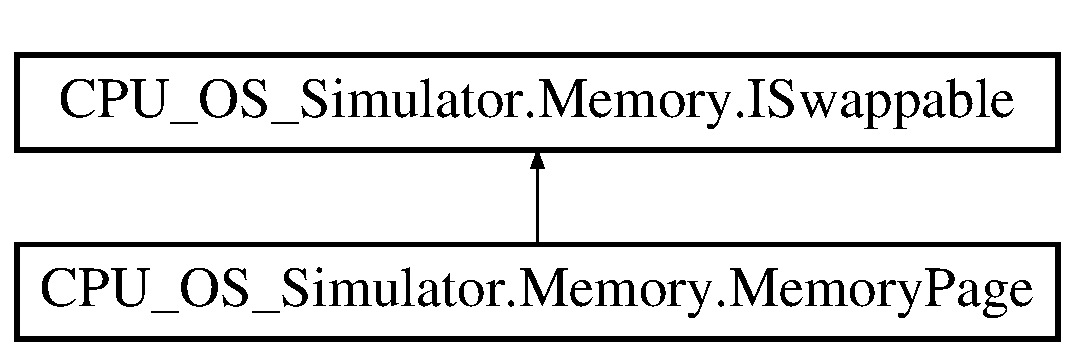
\includegraphics[height=2.000000cm]{class_c_p_u___o_s___simulator_1_1_memory_1_1_memory_page}
\end{center}
\end{figure}
\subsection*{Public Member Functions}
\begin{DoxyCompactItemize}
\item 
\hyperlink{class_c_p_u___o_s___simulator_1_1_memory_1_1_memory_page_a9b162033b9c9cc4dd28d683706fe6d2e}{Memory\+Page} (int \hyperlink{class_c_p_u___o_s___simulator_1_1_memory_1_1_memory_page_acf60a7bdefab6120fe080854b5f0b38b}{page\+Index}, int \hyperlink{class_c_p_u___o_s___simulator_1_1_memory_1_1_memory_page_a6fe2e28385db19a1968a41efe3df3f38}{start\+Offset})
\begin{DoxyCompactList}\small\item\em Constructor for memory page \end{DoxyCompactList}\item 
void \hyperlink{class_c_p_u___o_s___simulator_1_1_memory_1_1_memory_page_a53d6deee146e06754ea770755b17ff14}{Swap\+Out} (int Location\+To\+Swap, int Frame\+Number)
\begin{DoxyCompactList}\small\item\em This function swaps out this memory page \end{DoxyCompactList}\item 
void \hyperlink{class_c_p_u___o_s___simulator_1_1_memory_1_1_memory_page_a79e408c1be5efbaa6969ab66cc46930f}{Swap\+In} (int Location\+To\+Swap, int Frame\+Number)
\begin{DoxyCompactList}\small\item\em This function swaps in this memory page \end{DoxyCompactList}\item 
void \hyperlink{class_c_p_u___o_s___simulator_1_1_memory_1_1_memory_page_a0c43cf3b2640f17b8d732acbaaaead96}{Zero\+Memory} ()
\begin{DoxyCompactList}\small\item\em This function zeros out (clears) a memory page \end{DoxyCompactList}\end{DoxyCompactItemize}
\subsection*{Public Attributes}
\begin{DoxyCompactItemize}
\item 
const int \hyperlink{class_c_p_u___o_s___simulator_1_1_memory_1_1_memory_page_a502abee83030136a808d5b5f0c0fe7ec}{P\+A\+G\+E\+\_\+\+S\+I\+Z\+E} = 256
\begin{DoxyCompactList}\small\item\em The size of the memory pages to manage \end{DoxyCompactList}\end{DoxyCompactItemize}
\subsection*{Properties}
\begin{DoxyCompactItemize}
\item 
int \hyperlink{class_c_p_u___o_s___simulator_1_1_memory_1_1_memory_page_aec80700d036a447e7e6ec204513e3a59}{Page\+Index}\hspace{0.3cm}{\ttfamily  \mbox{[}get, set\mbox{]}}
\begin{DoxyCompactList}\small\item\em The index of the current page within its program \end{DoxyCompactList}\item 
int \hyperlink{class_c_p_u___o_s___simulator_1_1_memory_1_1_memory_page_ad700979e51dd3d05470c681588c6fa79}{Start\+Offset}\hspace{0.3cm}{\ttfamily  \mbox{[}get\mbox{]}}
\begin{DoxyCompactList}\small\item\em The start offset of this page \end{DoxyCompactList}\item 
int \hyperlink{class_c_p_u___o_s___simulator_1_1_memory_1_1_memory_page_abe850b4a088a820ecf598af1cd9a7deb}{End\+Offset}\hspace{0.3cm}{\ttfamily  \mbox{[}get\mbox{]}}
\begin{DoxyCompactList}\small\item\em the end offset of this page \end{DoxyCompactList}\item 
\hyperlink{class_c_p_u___o_s___simulator_1_1_memory_1_1_memory_segment}{Memory\+Segment}\mbox{[}$\,$\mbox{]} \hyperlink{class_c_p_u___o_s___simulator_1_1_memory_1_1_memory_page_a8bf84e82146f9ff35ffbcc32b93a9db0}{Data}\hspace{0.3cm}{\ttfamily  \mbox{[}get, set\mbox{]}}
\begin{DoxyCompactList}\small\item\em array of memory segments which collectively make up this page \end{DoxyCompactList}\item 
int \hyperlink{class_c_p_u___o_s___simulator_1_1_memory_1_1_memory_page_af31a2243a3e68ec635315929859fa358}{Start\+Offset\+Physical}\hspace{0.3cm}{\ttfamily  \mbox{[}get, set\mbox{]}}
\begin{DoxyCompactList}\small\item\em The physical address of the first byte in the page \end{DoxyCompactList}\end{DoxyCompactItemize}
\subsection*{Private Member Functions}
\begin{DoxyCompactItemize}
\item 
void \hyperlink{class_c_p_u___o_s___simulator_1_1_memory_1_1_memory_page_a4006da1460cb3bf17076dfbade9d0038}{Populate\+Data} ()
\begin{DoxyCompactList}\small\item\em Populates the data in this page with its initial value (0) \end{DoxyCompactList}\item 
dynamic \hyperlink{class_c_p_u___o_s___simulator_1_1_memory_1_1_memory_page_a84a305171941df5c3ae72b34ccec5485}{Get\+Main\+Window\+Instance} ()
\begin{DoxyCompactList}\small\item\em This function gets the main window instance from the window bridge \end{DoxyCompactList}\end{DoxyCompactItemize}
\subsection*{Private Attributes}
\begin{DoxyCompactItemize}
\item 
int \hyperlink{class_c_p_u___o_s___simulator_1_1_memory_1_1_memory_page_acf60a7bdefab6120fe080854b5f0b38b}{page\+Index}
\item 
int \hyperlink{class_c_p_u___o_s___simulator_1_1_memory_1_1_memory_page_a3cecfb0fe2f91def3db5711180442d44}{start\+Offset\+Physical}
\item 
readonly int \hyperlink{class_c_p_u___o_s___simulator_1_1_memory_1_1_memory_page_a6fe2e28385db19a1968a41efe3df3f38}{start\+Offset}
\item 
readonly int \hyperlink{class_c_p_u___o_s___simulator_1_1_memory_1_1_memory_page_ae2f8f419909326ce5449d37af9ff7c89}{end\+Offset}
\item 
\hyperlink{class_c_p_u___o_s___simulator_1_1_memory_1_1_memory_segment}{Memory\+Segment}\mbox{[}$\,$\mbox{]} \hyperlink{class_c_p_u___o_s___simulator_1_1_memory_1_1_memory_page_af9ab25101e7920de2344e0fa5ddfaa27}{data}
\end{DoxyCompactItemize}


\subsection{Detailed Description}
This class represents a page of data within memory 



Definition at line 10 of file Memory\+Page.\+cs.



\subsection{Constructor \& Destructor Documentation}
\hypertarget{class_c_p_u___o_s___simulator_1_1_memory_1_1_memory_page_a9b162033b9c9cc4dd28d683706fe6d2e}{}\index{C\+P\+U\+\_\+\+O\+S\+\_\+\+Simulator\+::\+Memory\+::\+Memory\+Page@{C\+P\+U\+\_\+\+O\+S\+\_\+\+Simulator\+::\+Memory\+::\+Memory\+Page}!Memory\+Page@{Memory\+Page}}
\index{Memory\+Page@{Memory\+Page}!C\+P\+U\+\_\+\+O\+S\+\_\+\+Simulator\+::\+Memory\+::\+Memory\+Page@{C\+P\+U\+\_\+\+O\+S\+\_\+\+Simulator\+::\+Memory\+::\+Memory\+Page}}
\subsubsection[{Memory\+Page(int page\+Index, int start\+Offset)}]{\setlength{\rightskip}{0pt plus 5cm}C\+P\+U\+\_\+\+O\+S\+\_\+\+Simulator.\+Memory.\+Memory\+Page.\+Memory\+Page (
\begin{DoxyParamCaption}
\item[{int}]{page\+Index, }
\item[{int}]{start\+Offset}
\end{DoxyParamCaption}
)}\label{class_c_p_u___o_s___simulator_1_1_memory_1_1_memory_page_a9b162033b9c9cc4dd28d683706fe6d2e}


Constructor for memory page 


\begin{DoxyParams}{Parameters}
{\em page\+Index} & the index of the page within the program\\
\hline
{\em start\+Offset} & \\
\hline
\end{DoxyParams}


Definition at line 93 of file Memory\+Page.\+cs.



\subsection{Member Function Documentation}
\hypertarget{class_c_p_u___o_s___simulator_1_1_memory_1_1_memory_page_a84a305171941df5c3ae72b34ccec5485}{}\index{C\+P\+U\+\_\+\+O\+S\+\_\+\+Simulator\+::\+Memory\+::\+Memory\+Page@{C\+P\+U\+\_\+\+O\+S\+\_\+\+Simulator\+::\+Memory\+::\+Memory\+Page}!Get\+Main\+Window\+Instance@{Get\+Main\+Window\+Instance}}
\index{Get\+Main\+Window\+Instance@{Get\+Main\+Window\+Instance}!C\+P\+U\+\_\+\+O\+S\+\_\+\+Simulator\+::\+Memory\+::\+Memory\+Page@{C\+P\+U\+\_\+\+O\+S\+\_\+\+Simulator\+::\+Memory\+::\+Memory\+Page}}
\subsubsection[{Get\+Main\+Window\+Instance()}]{\setlength{\rightskip}{0pt plus 5cm}dynamic C\+P\+U\+\_\+\+O\+S\+\_\+\+Simulator.\+Memory.\+Memory\+Page.\+Get\+Main\+Window\+Instance (
\begin{DoxyParamCaption}
{}
\end{DoxyParamCaption}
)\hspace{0.3cm}{\ttfamily [private]}}\label{class_c_p_u___o_s___simulator_1_1_memory_1_1_memory_page_a84a305171941df5c3ae72b34ccec5485}


This function gets the main window instance from the window bridge 

\begin{DoxyReturn}{Returns}
the active instance of main window 
\end{DoxyReturn}


Definition at line 170 of file Memory\+Page.\+cs.

\hypertarget{class_c_p_u___o_s___simulator_1_1_memory_1_1_memory_page_a4006da1460cb3bf17076dfbade9d0038}{}\index{C\+P\+U\+\_\+\+O\+S\+\_\+\+Simulator\+::\+Memory\+::\+Memory\+Page@{C\+P\+U\+\_\+\+O\+S\+\_\+\+Simulator\+::\+Memory\+::\+Memory\+Page}!Populate\+Data@{Populate\+Data}}
\index{Populate\+Data@{Populate\+Data}!C\+P\+U\+\_\+\+O\+S\+\_\+\+Simulator\+::\+Memory\+::\+Memory\+Page@{C\+P\+U\+\_\+\+O\+S\+\_\+\+Simulator\+::\+Memory\+::\+Memory\+Page}}
\subsubsection[{Populate\+Data()}]{\setlength{\rightskip}{0pt plus 5cm}void C\+P\+U\+\_\+\+O\+S\+\_\+\+Simulator.\+Memory.\+Memory\+Page.\+Populate\+Data (
\begin{DoxyParamCaption}
{}
\end{DoxyParamCaption}
)\hspace{0.3cm}{\ttfamily [private]}}\label{class_c_p_u___o_s___simulator_1_1_memory_1_1_memory_page_a4006da1460cb3bf17076dfbade9d0038}


Populates the data in this page with its initial value (0) 



Definition at line 106 of file Memory\+Page.\+cs.

\hypertarget{class_c_p_u___o_s___simulator_1_1_memory_1_1_memory_page_a79e408c1be5efbaa6969ab66cc46930f}{}\index{C\+P\+U\+\_\+\+O\+S\+\_\+\+Simulator\+::\+Memory\+::\+Memory\+Page@{C\+P\+U\+\_\+\+O\+S\+\_\+\+Simulator\+::\+Memory\+::\+Memory\+Page}!Swap\+In@{Swap\+In}}
\index{Swap\+In@{Swap\+In}!C\+P\+U\+\_\+\+O\+S\+\_\+\+Simulator\+::\+Memory\+::\+Memory\+Page@{C\+P\+U\+\_\+\+O\+S\+\_\+\+Simulator\+::\+Memory\+::\+Memory\+Page}}
\subsubsection[{Swap\+In(int Location\+To\+Swap, int Frame\+Number)}]{\setlength{\rightskip}{0pt plus 5cm}void C\+P\+U\+\_\+\+O\+S\+\_\+\+Simulator.\+Memory.\+Memory\+Page.\+Swap\+In (
\begin{DoxyParamCaption}
\item[{int}]{Location\+To\+Swap, }
\item[{int}]{Frame\+Number}
\end{DoxyParamCaption}
)}\label{class_c_p_u___o_s___simulator_1_1_memory_1_1_memory_page_a79e408c1be5efbaa6969ab66cc46930f}


This function swaps in this memory page 


\begin{DoxyParams}{Parameters}
{\em Location\+To\+Swap} & the physical address to swap this page in to\\
\hline
{\em Frame\+Number} & this pages frame number\\
\hline
\end{DoxyParams}


Implements \hyperlink{interface_c_p_u___o_s___simulator_1_1_memory_1_1_i_swappable_a38e30363486a3de53e6171da50b943af}{C\+P\+U\+\_\+\+O\+S\+\_\+\+Simulator.\+Memory.\+I\+Swappable}.



Definition at line 146 of file Memory\+Page.\+cs.

\hypertarget{class_c_p_u___o_s___simulator_1_1_memory_1_1_memory_page_a53d6deee146e06754ea770755b17ff14}{}\index{C\+P\+U\+\_\+\+O\+S\+\_\+\+Simulator\+::\+Memory\+::\+Memory\+Page@{C\+P\+U\+\_\+\+O\+S\+\_\+\+Simulator\+::\+Memory\+::\+Memory\+Page}!Swap\+Out@{Swap\+Out}}
\index{Swap\+Out@{Swap\+Out}!C\+P\+U\+\_\+\+O\+S\+\_\+\+Simulator\+::\+Memory\+::\+Memory\+Page@{C\+P\+U\+\_\+\+O\+S\+\_\+\+Simulator\+::\+Memory\+::\+Memory\+Page}}
\subsubsection[{Swap\+Out(int Location\+To\+Swap, int Frame\+Number)}]{\setlength{\rightskip}{0pt plus 5cm}void C\+P\+U\+\_\+\+O\+S\+\_\+\+Simulator.\+Memory.\+Memory\+Page.\+Swap\+Out (
\begin{DoxyParamCaption}
\item[{int}]{Location\+To\+Swap, }
\item[{int}]{Frame\+Number}
\end{DoxyParamCaption}
)}\label{class_c_p_u___o_s___simulator_1_1_memory_1_1_memory_page_a53d6deee146e06754ea770755b17ff14}


This function swaps out this memory page 


\begin{DoxyParams}{Parameters}
{\em Location\+To\+Swap} & the physical address to swap from\\
\hline
{\em Frame\+Number} & this page\textquotesingle{}s frame number\\
\hline
\end{DoxyParams}


Implements \hyperlink{interface_c_p_u___o_s___simulator_1_1_memory_1_1_i_swappable_ae789e9deb0600d48b0dcbe4a4252220a}{C\+P\+U\+\_\+\+O\+S\+\_\+\+Simulator.\+Memory.\+I\+Swappable}.



Definition at line 121 of file Memory\+Page.\+cs.

\hypertarget{class_c_p_u___o_s___simulator_1_1_memory_1_1_memory_page_a0c43cf3b2640f17b8d732acbaaaead96}{}\index{C\+P\+U\+\_\+\+O\+S\+\_\+\+Simulator\+::\+Memory\+::\+Memory\+Page@{C\+P\+U\+\_\+\+O\+S\+\_\+\+Simulator\+::\+Memory\+::\+Memory\+Page}!Zero\+Memory@{Zero\+Memory}}
\index{Zero\+Memory@{Zero\+Memory}!C\+P\+U\+\_\+\+O\+S\+\_\+\+Simulator\+::\+Memory\+::\+Memory\+Page@{C\+P\+U\+\_\+\+O\+S\+\_\+\+Simulator\+::\+Memory\+::\+Memory\+Page}}
\subsubsection[{Zero\+Memory()}]{\setlength{\rightskip}{0pt plus 5cm}void C\+P\+U\+\_\+\+O\+S\+\_\+\+Simulator.\+Memory.\+Memory\+Page.\+Zero\+Memory (
\begin{DoxyParamCaption}
{}
\end{DoxyParamCaption}
)}\label{class_c_p_u___o_s___simulator_1_1_memory_1_1_memory_page_a0c43cf3b2640f17b8d732acbaaaead96}


This function zeros out (clears) a memory page 



Definition at line 181 of file Memory\+Page.\+cs.



\subsection{Member Data Documentation}
\hypertarget{class_c_p_u___o_s___simulator_1_1_memory_1_1_memory_page_af9ab25101e7920de2344e0fa5ddfaa27}{}\index{C\+P\+U\+\_\+\+O\+S\+\_\+\+Simulator\+::\+Memory\+::\+Memory\+Page@{C\+P\+U\+\_\+\+O\+S\+\_\+\+Simulator\+::\+Memory\+::\+Memory\+Page}!data@{data}}
\index{data@{data}!C\+P\+U\+\_\+\+O\+S\+\_\+\+Simulator\+::\+Memory\+::\+Memory\+Page@{C\+P\+U\+\_\+\+O\+S\+\_\+\+Simulator\+::\+Memory\+::\+Memory\+Page}}
\subsubsection[{data}]{\setlength{\rightskip}{0pt plus 5cm}{\bf Memory\+Segment} \mbox{[}$\,$\mbox{]} C\+P\+U\+\_\+\+O\+S\+\_\+\+Simulator.\+Memory.\+Memory\+Page.\+data\hspace{0.3cm}{\ttfamily [private]}}\label{class_c_p_u___o_s___simulator_1_1_memory_1_1_memory_page_af9ab25101e7920de2344e0fa5ddfaa27}


Definition at line 20 of file Memory\+Page.\+cs.

\hypertarget{class_c_p_u___o_s___simulator_1_1_memory_1_1_memory_page_ae2f8f419909326ce5449d37af9ff7c89}{}\index{C\+P\+U\+\_\+\+O\+S\+\_\+\+Simulator\+::\+Memory\+::\+Memory\+Page@{C\+P\+U\+\_\+\+O\+S\+\_\+\+Simulator\+::\+Memory\+::\+Memory\+Page}!end\+Offset@{end\+Offset}}
\index{end\+Offset@{end\+Offset}!C\+P\+U\+\_\+\+O\+S\+\_\+\+Simulator\+::\+Memory\+::\+Memory\+Page@{C\+P\+U\+\_\+\+O\+S\+\_\+\+Simulator\+::\+Memory\+::\+Memory\+Page}}
\subsubsection[{end\+Offset}]{\setlength{\rightskip}{0pt plus 5cm}readonly int C\+P\+U\+\_\+\+O\+S\+\_\+\+Simulator.\+Memory.\+Memory\+Page.\+end\+Offset\hspace{0.3cm}{\ttfamily [private]}}\label{class_c_p_u___o_s___simulator_1_1_memory_1_1_memory_page_ae2f8f419909326ce5449d37af9ff7c89}


Definition at line 19 of file Memory\+Page.\+cs.

\hypertarget{class_c_p_u___o_s___simulator_1_1_memory_1_1_memory_page_a502abee83030136a808d5b5f0c0fe7ec}{}\index{C\+P\+U\+\_\+\+O\+S\+\_\+\+Simulator\+::\+Memory\+::\+Memory\+Page@{C\+P\+U\+\_\+\+O\+S\+\_\+\+Simulator\+::\+Memory\+::\+Memory\+Page}!P\+A\+G\+E\+\_\+\+S\+I\+Z\+E@{P\+A\+G\+E\+\_\+\+S\+I\+Z\+E}}
\index{P\+A\+G\+E\+\_\+\+S\+I\+Z\+E@{P\+A\+G\+E\+\_\+\+S\+I\+Z\+E}!C\+P\+U\+\_\+\+O\+S\+\_\+\+Simulator\+::\+Memory\+::\+Memory\+Page@{C\+P\+U\+\_\+\+O\+S\+\_\+\+Simulator\+::\+Memory\+::\+Memory\+Page}}
\subsubsection[{P\+A\+G\+E\+\_\+\+S\+I\+Z\+E}]{\setlength{\rightskip}{0pt plus 5cm}const int C\+P\+U\+\_\+\+O\+S\+\_\+\+Simulator.\+Memory.\+Memory\+Page.\+P\+A\+G\+E\+\_\+\+S\+I\+Z\+E = 256}\label{class_c_p_u___o_s___simulator_1_1_memory_1_1_memory_page_a502abee83030136a808d5b5f0c0fe7ec}


The size of the memory pages to manage 



Definition at line 18 of file Memory\+Page.\+cs.

\hypertarget{class_c_p_u___o_s___simulator_1_1_memory_1_1_memory_page_acf60a7bdefab6120fe080854b5f0b38b}{}\index{C\+P\+U\+\_\+\+O\+S\+\_\+\+Simulator\+::\+Memory\+::\+Memory\+Page@{C\+P\+U\+\_\+\+O\+S\+\_\+\+Simulator\+::\+Memory\+::\+Memory\+Page}!page\+Index@{page\+Index}}
\index{page\+Index@{page\+Index}!C\+P\+U\+\_\+\+O\+S\+\_\+\+Simulator\+::\+Memory\+::\+Memory\+Page@{C\+P\+U\+\_\+\+O\+S\+\_\+\+Simulator\+::\+Memory\+::\+Memory\+Page}}
\subsubsection[{page\+Index}]{\setlength{\rightskip}{0pt plus 5cm}int C\+P\+U\+\_\+\+O\+S\+\_\+\+Simulator.\+Memory.\+Memory\+Page.\+page\+Index\hspace{0.3cm}{\ttfamily [private]}}\label{class_c_p_u___o_s___simulator_1_1_memory_1_1_memory_page_acf60a7bdefab6120fe080854b5f0b38b}


Definition at line 12 of file Memory\+Page.\+cs.

\hypertarget{class_c_p_u___o_s___simulator_1_1_memory_1_1_memory_page_a6fe2e28385db19a1968a41efe3df3f38}{}\index{C\+P\+U\+\_\+\+O\+S\+\_\+\+Simulator\+::\+Memory\+::\+Memory\+Page@{C\+P\+U\+\_\+\+O\+S\+\_\+\+Simulator\+::\+Memory\+::\+Memory\+Page}!start\+Offset@{start\+Offset}}
\index{start\+Offset@{start\+Offset}!C\+P\+U\+\_\+\+O\+S\+\_\+\+Simulator\+::\+Memory\+::\+Memory\+Page@{C\+P\+U\+\_\+\+O\+S\+\_\+\+Simulator\+::\+Memory\+::\+Memory\+Page}}
\subsubsection[{start\+Offset}]{\setlength{\rightskip}{0pt plus 5cm}readonly int C\+P\+U\+\_\+\+O\+S\+\_\+\+Simulator.\+Memory.\+Memory\+Page.\+start\+Offset\hspace{0.3cm}{\ttfamily [private]}}\label{class_c_p_u___o_s___simulator_1_1_memory_1_1_memory_page_a6fe2e28385db19a1968a41efe3df3f38}


Definition at line 14 of file Memory\+Page.\+cs.

\hypertarget{class_c_p_u___o_s___simulator_1_1_memory_1_1_memory_page_a3cecfb0fe2f91def3db5711180442d44}{}\index{C\+P\+U\+\_\+\+O\+S\+\_\+\+Simulator\+::\+Memory\+::\+Memory\+Page@{C\+P\+U\+\_\+\+O\+S\+\_\+\+Simulator\+::\+Memory\+::\+Memory\+Page}!start\+Offset\+Physical@{start\+Offset\+Physical}}
\index{start\+Offset\+Physical@{start\+Offset\+Physical}!C\+P\+U\+\_\+\+O\+S\+\_\+\+Simulator\+::\+Memory\+::\+Memory\+Page@{C\+P\+U\+\_\+\+O\+S\+\_\+\+Simulator\+::\+Memory\+::\+Memory\+Page}}
\subsubsection[{start\+Offset\+Physical}]{\setlength{\rightskip}{0pt plus 5cm}int C\+P\+U\+\_\+\+O\+S\+\_\+\+Simulator.\+Memory.\+Memory\+Page.\+start\+Offset\+Physical\hspace{0.3cm}{\ttfamily [private]}}\label{class_c_p_u___o_s___simulator_1_1_memory_1_1_memory_page_a3cecfb0fe2f91def3db5711180442d44}


Definition at line 13 of file Memory\+Page.\+cs.



\subsection{Property Documentation}
\hypertarget{class_c_p_u___o_s___simulator_1_1_memory_1_1_memory_page_a8bf84e82146f9ff35ffbcc32b93a9db0}{}\index{C\+P\+U\+\_\+\+O\+S\+\_\+\+Simulator\+::\+Memory\+::\+Memory\+Page@{C\+P\+U\+\_\+\+O\+S\+\_\+\+Simulator\+::\+Memory\+::\+Memory\+Page}!Data@{Data}}
\index{Data@{Data}!C\+P\+U\+\_\+\+O\+S\+\_\+\+Simulator\+::\+Memory\+::\+Memory\+Page@{C\+P\+U\+\_\+\+O\+S\+\_\+\+Simulator\+::\+Memory\+::\+Memory\+Page}}
\subsubsection[{Data}]{\setlength{\rightskip}{0pt plus 5cm}{\bf Memory\+Segment} \mbox{[}$\,$\mbox{]} C\+P\+U\+\_\+\+O\+S\+\_\+\+Simulator.\+Memory.\+Memory\+Page.\+Data\hspace{0.3cm}{\ttfamily [get]}, {\ttfamily [set]}}\label{class_c_p_u___o_s___simulator_1_1_memory_1_1_memory_page_a8bf84e82146f9ff35ffbcc32b93a9db0}


array of memory segments which collectively make up this page 



Definition at line 60 of file Memory\+Page.\+cs.

\hypertarget{class_c_p_u___o_s___simulator_1_1_memory_1_1_memory_page_abe850b4a088a820ecf598af1cd9a7deb}{}\index{C\+P\+U\+\_\+\+O\+S\+\_\+\+Simulator\+::\+Memory\+::\+Memory\+Page@{C\+P\+U\+\_\+\+O\+S\+\_\+\+Simulator\+::\+Memory\+::\+Memory\+Page}!End\+Offset@{End\+Offset}}
\index{End\+Offset@{End\+Offset}!C\+P\+U\+\_\+\+O\+S\+\_\+\+Simulator\+::\+Memory\+::\+Memory\+Page@{C\+P\+U\+\_\+\+O\+S\+\_\+\+Simulator\+::\+Memory\+::\+Memory\+Page}}
\subsubsection[{End\+Offset}]{\setlength{\rightskip}{0pt plus 5cm}int C\+P\+U\+\_\+\+O\+S\+\_\+\+Simulator.\+Memory.\+Memory\+Page.\+End\+Offset\hspace{0.3cm}{\ttfamily [get]}}\label{class_c_p_u___o_s___simulator_1_1_memory_1_1_memory_page_abe850b4a088a820ecf598af1cd9a7deb}


the end offset of this page 



Definition at line 50 of file Memory\+Page.\+cs.

\hypertarget{class_c_p_u___o_s___simulator_1_1_memory_1_1_memory_page_aec80700d036a447e7e6ec204513e3a59}{}\index{C\+P\+U\+\_\+\+O\+S\+\_\+\+Simulator\+::\+Memory\+::\+Memory\+Page@{C\+P\+U\+\_\+\+O\+S\+\_\+\+Simulator\+::\+Memory\+::\+Memory\+Page}!Page\+Index@{Page\+Index}}
\index{Page\+Index@{Page\+Index}!C\+P\+U\+\_\+\+O\+S\+\_\+\+Simulator\+::\+Memory\+::\+Memory\+Page@{C\+P\+U\+\_\+\+O\+S\+\_\+\+Simulator\+::\+Memory\+::\+Memory\+Page}}
\subsubsection[{Page\+Index}]{\setlength{\rightskip}{0pt plus 5cm}int C\+P\+U\+\_\+\+O\+S\+\_\+\+Simulator.\+Memory.\+Memory\+Page.\+Page\+Index\hspace{0.3cm}{\ttfamily [get]}, {\ttfamily [set]}}\label{class_c_p_u___o_s___simulator_1_1_memory_1_1_memory_page_aec80700d036a447e7e6ec204513e3a59}


The index of the current page within its program 



Definition at line 25 of file Memory\+Page.\+cs.

\hypertarget{class_c_p_u___o_s___simulator_1_1_memory_1_1_memory_page_ad700979e51dd3d05470c681588c6fa79}{}\index{C\+P\+U\+\_\+\+O\+S\+\_\+\+Simulator\+::\+Memory\+::\+Memory\+Page@{C\+P\+U\+\_\+\+O\+S\+\_\+\+Simulator\+::\+Memory\+::\+Memory\+Page}!Start\+Offset@{Start\+Offset}}
\index{Start\+Offset@{Start\+Offset}!C\+P\+U\+\_\+\+O\+S\+\_\+\+Simulator\+::\+Memory\+::\+Memory\+Page@{C\+P\+U\+\_\+\+O\+S\+\_\+\+Simulator\+::\+Memory\+::\+Memory\+Page}}
\subsubsection[{Start\+Offset}]{\setlength{\rightskip}{0pt plus 5cm}int C\+P\+U\+\_\+\+O\+S\+\_\+\+Simulator.\+Memory.\+Memory\+Page.\+Start\+Offset\hspace{0.3cm}{\ttfamily [get]}}\label{class_c_p_u___o_s___simulator_1_1_memory_1_1_memory_page_ad700979e51dd3d05470c681588c6fa79}


The start offset of this page 



Definition at line 40 of file Memory\+Page.\+cs.

\hypertarget{class_c_p_u___o_s___simulator_1_1_memory_1_1_memory_page_af31a2243a3e68ec635315929859fa358}{}\index{C\+P\+U\+\_\+\+O\+S\+\_\+\+Simulator\+::\+Memory\+::\+Memory\+Page@{C\+P\+U\+\_\+\+O\+S\+\_\+\+Simulator\+::\+Memory\+::\+Memory\+Page}!Start\+Offset\+Physical@{Start\+Offset\+Physical}}
\index{Start\+Offset\+Physical@{Start\+Offset\+Physical}!C\+P\+U\+\_\+\+O\+S\+\_\+\+Simulator\+::\+Memory\+::\+Memory\+Page@{C\+P\+U\+\_\+\+O\+S\+\_\+\+Simulator\+::\+Memory\+::\+Memory\+Page}}
\subsubsection[{Start\+Offset\+Physical}]{\setlength{\rightskip}{0pt plus 5cm}int C\+P\+U\+\_\+\+O\+S\+\_\+\+Simulator.\+Memory.\+Memory\+Page.\+Start\+Offset\+Physical\hspace{0.3cm}{\ttfamily [get]}, {\ttfamily [set]}}\label{class_c_p_u___o_s___simulator_1_1_memory_1_1_memory_page_af31a2243a3e68ec635315929859fa358}


The physical address of the first byte in the page 



Definition at line 75 of file Memory\+Page.\+cs.



The documentation for this class was generated from the following file\+:\begin{DoxyCompactItemize}
\item 
Memory/\hyperlink{_memory_page_8cs}{Memory\+Page.\+cs}\end{DoxyCompactItemize}

\hypertarget{class_c_p_u___o_s___simulator_1_1_c_p_u_1_1_number_of_operands_attribute}{}\section{C\+P\+U\+\_\+\+O\+S\+\_\+\+Simulator.\+C\+P\+U.\+Number\+Of\+Operands\+Attribute Class Reference}
\label{class_c_p_u___o_s___simulator_1_1_c_p_u_1_1_number_of_operands_attribute}\index{C\+P\+U\+\_\+\+O\+S\+\_\+\+Simulator.\+C\+P\+U.\+Number\+Of\+Operands\+Attribute@{C\+P\+U\+\_\+\+O\+S\+\_\+\+Simulator.\+C\+P\+U.\+Number\+Of\+Operands\+Attribute}}


This class represents the Number\+Of\+Operands attribute  


Inheritance diagram for C\+P\+U\+\_\+\+O\+S\+\_\+\+Simulator.\+C\+P\+U.\+Number\+Of\+Operands\+Attribute\+:\begin{figure}[H]
\begin{center}
\leavevmode
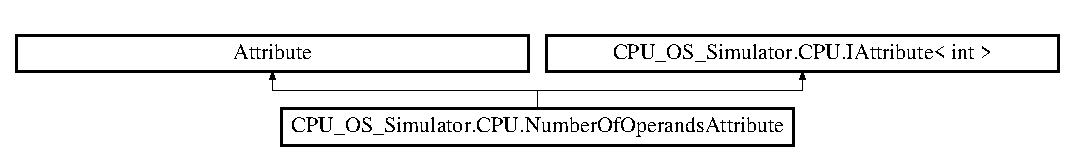
\includegraphics[height=1.733746cm]{class_c_p_u___o_s___simulator_1_1_c_p_u_1_1_number_of_operands_attribute}
\end{center}
\end{figure}
\subsection*{Public Member Functions}
\begin{DoxyCompactItemize}
\item 
\hyperlink{class_c_p_u___o_s___simulator_1_1_c_p_u_1_1_number_of_operands_attribute_a1976902af3b6dc92e16724d83937816e}{Number\+Of\+Operands\+Attribute} (int \hyperlink{class_c_p_u___o_s___simulator_1_1_c_p_u_1_1_number_of_operands_attribute_a23e7e9d6f0e3af1c7deddce153d13965}{value})
\begin{DoxyCompactList}\small\item\em Constructor for the Number\+O\+F\+Operands attribute \end{DoxyCompactList}\end{DoxyCompactItemize}
\subsection*{Properties}
\begin{DoxyCompactItemize}
\item 
int \hyperlink{class_c_p_u___o_s___simulator_1_1_c_p_u_1_1_number_of_operands_attribute_a00873634b211bcf2fd8b1425aa5143d6}{Value}\hspace{0.3cm}{\ttfamily  \mbox{[}get\mbox{]}}
\begin{DoxyCompactList}\small\item\em Property for the value of the attribute \end{DoxyCompactList}\end{DoxyCompactItemize}
\subsection*{Private Attributes}
\begin{DoxyCompactItemize}
\item 
readonly int \hyperlink{class_c_p_u___o_s___simulator_1_1_c_p_u_1_1_number_of_operands_attribute_a23e7e9d6f0e3af1c7deddce153d13965}{value}
\begin{DoxyCompactList}\small\item\em The value of the attribute \end{DoxyCompactList}\end{DoxyCompactItemize}


\subsection{Detailed Description}
This class represents the Number\+Of\+Operands attribute 



Definition at line 8 of file Number\+Of\+Operands\+Attribute.\+cs.



\subsection{Constructor \& Destructor Documentation}
\hypertarget{class_c_p_u___o_s___simulator_1_1_c_p_u_1_1_number_of_operands_attribute_a1976902af3b6dc92e16724d83937816e}{}\index{C\+P\+U\+\_\+\+O\+S\+\_\+\+Simulator\+::\+C\+P\+U\+::\+Number\+Of\+Operands\+Attribute@{C\+P\+U\+\_\+\+O\+S\+\_\+\+Simulator\+::\+C\+P\+U\+::\+Number\+Of\+Operands\+Attribute}!Number\+Of\+Operands\+Attribute@{Number\+Of\+Operands\+Attribute}}
\index{Number\+Of\+Operands\+Attribute@{Number\+Of\+Operands\+Attribute}!C\+P\+U\+\_\+\+O\+S\+\_\+\+Simulator\+::\+C\+P\+U\+::\+Number\+Of\+Operands\+Attribute@{C\+P\+U\+\_\+\+O\+S\+\_\+\+Simulator\+::\+C\+P\+U\+::\+Number\+Of\+Operands\+Attribute}}
\subsubsection[{Number\+Of\+Operands\+Attribute(int value)}]{\setlength{\rightskip}{0pt plus 5cm}C\+P\+U\+\_\+\+O\+S\+\_\+\+Simulator.\+C\+P\+U.\+Number\+Of\+Operands\+Attribute.\+Number\+Of\+Operands\+Attribute (
\begin{DoxyParamCaption}
\item[{int}]{value}
\end{DoxyParamCaption}
)}\label{class_c_p_u___o_s___simulator_1_1_c_p_u_1_1_number_of_operands_attribute_a1976902af3b6dc92e16724d83937816e}


Constructor for the Number\+O\+F\+Operands attribute 


\begin{DoxyParams}{Parameters}
{\em value} & the value to store in the attribute \\
\hline
\end{DoxyParams}


Definition at line 19 of file Number\+Of\+Operands\+Attribute.\+cs.



\subsection{Member Data Documentation}
\hypertarget{class_c_p_u___o_s___simulator_1_1_c_p_u_1_1_number_of_operands_attribute_a23e7e9d6f0e3af1c7deddce153d13965}{}\index{C\+P\+U\+\_\+\+O\+S\+\_\+\+Simulator\+::\+C\+P\+U\+::\+Number\+Of\+Operands\+Attribute@{C\+P\+U\+\_\+\+O\+S\+\_\+\+Simulator\+::\+C\+P\+U\+::\+Number\+Of\+Operands\+Attribute}!value@{value}}
\index{value@{value}!C\+P\+U\+\_\+\+O\+S\+\_\+\+Simulator\+::\+C\+P\+U\+::\+Number\+Of\+Operands\+Attribute@{C\+P\+U\+\_\+\+O\+S\+\_\+\+Simulator\+::\+C\+P\+U\+::\+Number\+Of\+Operands\+Attribute}}
\subsubsection[{value}]{\setlength{\rightskip}{0pt plus 5cm}readonly int C\+P\+U\+\_\+\+O\+S\+\_\+\+Simulator.\+C\+P\+U.\+Number\+Of\+Operands\+Attribute.\+value\hspace{0.3cm}{\ttfamily [private]}}\label{class_c_p_u___o_s___simulator_1_1_c_p_u_1_1_number_of_operands_attribute_a23e7e9d6f0e3af1c7deddce153d13965}


The value of the attribute 



Definition at line 13 of file Number\+Of\+Operands\+Attribute.\+cs.



\subsection{Property Documentation}
\hypertarget{class_c_p_u___o_s___simulator_1_1_c_p_u_1_1_number_of_operands_attribute_a00873634b211bcf2fd8b1425aa5143d6}{}\index{C\+P\+U\+\_\+\+O\+S\+\_\+\+Simulator\+::\+C\+P\+U\+::\+Number\+Of\+Operands\+Attribute@{C\+P\+U\+\_\+\+O\+S\+\_\+\+Simulator\+::\+C\+P\+U\+::\+Number\+Of\+Operands\+Attribute}!Value@{Value}}
\index{Value@{Value}!C\+P\+U\+\_\+\+O\+S\+\_\+\+Simulator\+::\+C\+P\+U\+::\+Number\+Of\+Operands\+Attribute@{C\+P\+U\+\_\+\+O\+S\+\_\+\+Simulator\+::\+C\+P\+U\+::\+Number\+Of\+Operands\+Attribute}}
\subsubsection[{Value}]{\setlength{\rightskip}{0pt plus 5cm}int C\+P\+U\+\_\+\+O\+S\+\_\+\+Simulator.\+C\+P\+U.\+Number\+Of\+Operands\+Attribute.\+Value\hspace{0.3cm}{\ttfamily [get]}}\label{class_c_p_u___o_s___simulator_1_1_c_p_u_1_1_number_of_operands_attribute_a00873634b211bcf2fd8b1425aa5143d6}


Property for the value of the attribute 



Definition at line 27 of file Number\+Of\+Operands\+Attribute.\+cs.



The documentation for this class was generated from the following file\+:\begin{DoxyCompactItemize}
\item 
C\+P\+U/\hyperlink{_number_of_operands_attribute_8cs}{Number\+Of\+Operands\+Attribute.\+cs}\end{DoxyCompactItemize}

\hypertarget{class_c_p_u___o_s___simulator_1_1_c_p_u_1_1_operand}{}\section{C\+P\+U\+\_\+\+O\+S\+\_\+\+Simulator.\+C\+P\+U.\+Operand Class Reference}
\label{class_c_p_u___o_s___simulator_1_1_c_p_u_1_1_operand}\index{C\+P\+U\+\_\+\+O\+S\+\_\+\+Simulator.\+C\+P\+U.\+Operand@{C\+P\+U\+\_\+\+O\+S\+\_\+\+Simulator.\+C\+P\+U.\+Operand}}


This class represents an operand which can be passed to an instruction  


\subsection*{Public Member Functions}
\begin{DoxyCompactItemize}
\item 
\hyperlink{class_c_p_u___o_s___simulator_1_1_c_p_u_1_1_operand_a8f6d642c2e5741c17748379c34a3052c}{Operand} ()
\begin{DoxyCompactList}\small\item\em Default constructor for an operand used when deserialising an operand N\+O\+T\+E do not use in code \end{DoxyCompactList}\item 
\hyperlink{class_c_p_u___o_s___simulator_1_1_c_p_u_1_1_operand_a66ce3c1acaa5f53e1f3af5276968b6e2}{Operand} (Int32 \hyperlink{class_c_p_u___o_s___simulator_1_1_c_p_u_1_1_operand_ab418a225965ed7e8d07649b218a7edd4}{value}, \hyperlink{namespace_c_p_u___o_s___simulator_1_1_c_p_u_ad49cfe442b74115a326c03b7ae848f76}{Enum\+Operand\+Type} \hyperlink{class_c_p_u___o_s___simulator_1_1_c_p_u_1_1_operand_abc8f504a22e9a5c49d91b12f61cc5119}{type})
\begin{DoxyCompactList}\small\item\em Constructor for an operand which is an intermediate value \end{DoxyCompactList}\item 
\hyperlink{class_c_p_u___o_s___simulator_1_1_c_p_u_1_1_operand_ab1da49c3f7978edcfa8c9b95e5804f08}{Operand} (\hyperlink{class_c_p_u___o_s___simulator_1_1_c_p_u_1_1_register}{Register} reg, \hyperlink{namespace_c_p_u___o_s___simulator_1_1_c_p_u_ad49cfe442b74115a326c03b7ae848f76}{Enum\+Operand\+Type} \hyperlink{class_c_p_u___o_s___simulator_1_1_c_p_u_1_1_operand_abc8f504a22e9a5c49d91b12f61cc5119}{type})
\begin{DoxyCompactList}\small\item\em Constructor for an operand which is a register \end{DoxyCompactList}\end{DoxyCompactItemize}
\subsection*{Properties}
\begin{DoxyCompactItemize}
\item 
int \hyperlink{class_c_p_u___o_s___simulator_1_1_c_p_u_1_1_operand_ab109292eba2094db4d7f21cbdbd5bc9e}{Value}\hspace{0.3cm}{\ttfamily  \mbox{[}get, set\mbox{]}}
\item 
\hyperlink{namespace_c_p_u___o_s___simulator_1_1_c_p_u_ad49cfe442b74115a326c03b7ae848f76}{Enum\+Operand\+Type} \hyperlink{class_c_p_u___o_s___simulator_1_1_c_p_u_1_1_operand_a0b0deae57b760df3a083dc54535b0891}{Type}\hspace{0.3cm}{\ttfamily  \mbox{[}get, set\mbox{]}}
\item 
bool \hyperlink{class_c_p_u___o_s___simulator_1_1_c_p_u_1_1_operand_a662aacb6eb1aa9cf818181aea695e0c9}{Is\+Register}\hspace{0.3cm}{\ttfamily  \mbox{[}get, set\mbox{]}}
\item 
\hyperlink{class_c_p_u___o_s___simulator_1_1_c_p_u_1_1_register}{Register} \hyperlink{class_c_p_u___o_s___simulator_1_1_c_p_u_1_1_operand_a8f08360f0e27922fc0377f5d58a9e67f}{Register}\hspace{0.3cm}{\ttfamily  \mbox{[}get, set\mbox{]}}
\end{DoxyCompactItemize}
\subsection*{Private Attributes}
\begin{DoxyCompactItemize}
\item 
Int32 \hyperlink{class_c_p_u___o_s___simulator_1_1_c_p_u_1_1_operand_ab418a225965ed7e8d07649b218a7edd4}{value}
\item 
\hyperlink{namespace_c_p_u___o_s___simulator_1_1_c_p_u_ad49cfe442b74115a326c03b7ae848f76}{Enum\+Operand\+Type} \hyperlink{class_c_p_u___o_s___simulator_1_1_c_p_u_1_1_operand_abc8f504a22e9a5c49d91b12f61cc5119}{type}
\item 
bool \hyperlink{class_c_p_u___o_s___simulator_1_1_c_p_u_1_1_operand_a16cc03d0d4c600b864d9c189529a473d}{is\+Register}
\item 
\hyperlink{class_c_p_u___o_s___simulator_1_1_c_p_u_1_1_register}{Register} \hyperlink{class_c_p_u___o_s___simulator_1_1_c_p_u_1_1_operand_a55d446765a50844fcbbc56b757b1b679}{register}
\end{DoxyCompactItemize}


\subsection{Detailed Description}
This class represents an operand which can be passed to an instruction 



Definition at line 9 of file Operand.\+cs.



\subsection{Constructor \& Destructor Documentation}
\hypertarget{class_c_p_u___o_s___simulator_1_1_c_p_u_1_1_operand_a8f6d642c2e5741c17748379c34a3052c}{}\index{C\+P\+U\+\_\+\+O\+S\+\_\+\+Simulator\+::\+C\+P\+U\+::\+Operand@{C\+P\+U\+\_\+\+O\+S\+\_\+\+Simulator\+::\+C\+P\+U\+::\+Operand}!Operand@{Operand}}
\index{Operand@{Operand}!C\+P\+U\+\_\+\+O\+S\+\_\+\+Simulator\+::\+C\+P\+U\+::\+Operand@{C\+P\+U\+\_\+\+O\+S\+\_\+\+Simulator\+::\+C\+P\+U\+::\+Operand}}
\subsubsection[{Operand()}]{\setlength{\rightskip}{0pt plus 5cm}C\+P\+U\+\_\+\+O\+S\+\_\+\+Simulator.\+C\+P\+U.\+Operand.\+Operand (
\begin{DoxyParamCaption}
{}
\end{DoxyParamCaption}
)}\label{class_c_p_u___o_s___simulator_1_1_c_p_u_1_1_operand_a8f6d642c2e5741c17748379c34a3052c}


Default constructor for an operand used when deserialising an operand N\+O\+T\+E do not use in code 



Definition at line 26 of file Operand.\+cs.

\hypertarget{class_c_p_u___o_s___simulator_1_1_c_p_u_1_1_operand_a66ce3c1acaa5f53e1f3af5276968b6e2}{}\index{C\+P\+U\+\_\+\+O\+S\+\_\+\+Simulator\+::\+C\+P\+U\+::\+Operand@{C\+P\+U\+\_\+\+O\+S\+\_\+\+Simulator\+::\+C\+P\+U\+::\+Operand}!Operand@{Operand}}
\index{Operand@{Operand}!C\+P\+U\+\_\+\+O\+S\+\_\+\+Simulator\+::\+C\+P\+U\+::\+Operand@{C\+P\+U\+\_\+\+O\+S\+\_\+\+Simulator\+::\+C\+P\+U\+::\+Operand}}
\subsubsection[{Operand(\+Int32 value, Enum\+Operand\+Type type)}]{\setlength{\rightskip}{0pt plus 5cm}C\+P\+U\+\_\+\+O\+S\+\_\+\+Simulator.\+C\+P\+U.\+Operand.\+Operand (
\begin{DoxyParamCaption}
\item[{Int32}]{value, }
\item[{{\bf Enum\+Operand\+Type}}]{type}
\end{DoxyParamCaption}
)}\label{class_c_p_u___o_s___simulator_1_1_c_p_u_1_1_operand_a66ce3c1acaa5f53e1f3af5276968b6e2}


Constructor for an operand which is an intermediate value 


\begin{DoxyParams}{Parameters}
{\em value} & the value of the operand \\
\hline
{\em type} & the type of the operand i.\+e memory address or intermediate value\\
\hline
\end{DoxyParams}


Definition at line 35 of file Operand.\+cs.

\hypertarget{class_c_p_u___o_s___simulator_1_1_c_p_u_1_1_operand_ab1da49c3f7978edcfa8c9b95e5804f08}{}\index{C\+P\+U\+\_\+\+O\+S\+\_\+\+Simulator\+::\+C\+P\+U\+::\+Operand@{C\+P\+U\+\_\+\+O\+S\+\_\+\+Simulator\+::\+C\+P\+U\+::\+Operand}!Operand@{Operand}}
\index{Operand@{Operand}!C\+P\+U\+\_\+\+O\+S\+\_\+\+Simulator\+::\+C\+P\+U\+::\+Operand@{C\+P\+U\+\_\+\+O\+S\+\_\+\+Simulator\+::\+C\+P\+U\+::\+Operand}}
\subsubsection[{Operand(\+Register reg, Enum\+Operand\+Type type)}]{\setlength{\rightskip}{0pt plus 5cm}C\+P\+U\+\_\+\+O\+S\+\_\+\+Simulator.\+C\+P\+U.\+Operand.\+Operand (
\begin{DoxyParamCaption}
\item[{{\bf Register}}]{reg, }
\item[{{\bf Enum\+Operand\+Type}}]{type}
\end{DoxyParamCaption}
)}\label{class_c_p_u___o_s___simulator_1_1_c_p_u_1_1_operand_ab1da49c3f7978edcfa8c9b95e5804f08}


Constructor for an operand which is a register 


\begin{DoxyParams}{Parameters}
{\em reg} & the register to be passed as an operand\\
\hline
{\em type} & the type of the operand i.\+e memory address or intermediate value\\
\hline
\end{DoxyParams}


Definition at line 48 of file Operand.\+cs.



\subsection{Member Data Documentation}
\hypertarget{class_c_p_u___o_s___simulator_1_1_c_p_u_1_1_operand_a16cc03d0d4c600b864d9c189529a473d}{}\index{C\+P\+U\+\_\+\+O\+S\+\_\+\+Simulator\+::\+C\+P\+U\+::\+Operand@{C\+P\+U\+\_\+\+O\+S\+\_\+\+Simulator\+::\+C\+P\+U\+::\+Operand}!is\+Register@{is\+Register}}
\index{is\+Register@{is\+Register}!C\+P\+U\+\_\+\+O\+S\+\_\+\+Simulator\+::\+C\+P\+U\+::\+Operand@{C\+P\+U\+\_\+\+O\+S\+\_\+\+Simulator\+::\+C\+P\+U\+::\+Operand}}
\subsubsection[{is\+Register}]{\setlength{\rightskip}{0pt plus 5cm}bool C\+P\+U\+\_\+\+O\+S\+\_\+\+Simulator.\+C\+P\+U.\+Operand.\+is\+Register\hspace{0.3cm}{\ttfamily [private]}}\label{class_c_p_u___o_s___simulator_1_1_c_p_u_1_1_operand_a16cc03d0d4c600b864d9c189529a473d}


Definition at line 15 of file Operand.\+cs.

\hypertarget{class_c_p_u___o_s___simulator_1_1_c_p_u_1_1_operand_a55d446765a50844fcbbc56b757b1b679}{}\index{C\+P\+U\+\_\+\+O\+S\+\_\+\+Simulator\+::\+C\+P\+U\+::\+Operand@{C\+P\+U\+\_\+\+O\+S\+\_\+\+Simulator\+::\+C\+P\+U\+::\+Operand}!register@{register}}
\index{register@{register}!C\+P\+U\+\_\+\+O\+S\+\_\+\+Simulator\+::\+C\+P\+U\+::\+Operand@{C\+P\+U\+\_\+\+O\+S\+\_\+\+Simulator\+::\+C\+P\+U\+::\+Operand}}
\subsubsection[{register}]{\setlength{\rightskip}{0pt plus 5cm}{\bf Register} C\+P\+U\+\_\+\+O\+S\+\_\+\+Simulator.\+C\+P\+U.\+Operand.\+register\hspace{0.3cm}{\ttfamily [private]}}\label{class_c_p_u___o_s___simulator_1_1_c_p_u_1_1_operand_a55d446765a50844fcbbc56b757b1b679}


Definition at line 16 of file Operand.\+cs.

\hypertarget{class_c_p_u___o_s___simulator_1_1_c_p_u_1_1_operand_abc8f504a22e9a5c49d91b12f61cc5119}{}\index{C\+P\+U\+\_\+\+O\+S\+\_\+\+Simulator\+::\+C\+P\+U\+::\+Operand@{C\+P\+U\+\_\+\+O\+S\+\_\+\+Simulator\+::\+C\+P\+U\+::\+Operand}!type@{type}}
\index{type@{type}!C\+P\+U\+\_\+\+O\+S\+\_\+\+Simulator\+::\+C\+P\+U\+::\+Operand@{C\+P\+U\+\_\+\+O\+S\+\_\+\+Simulator\+::\+C\+P\+U\+::\+Operand}}
\subsubsection[{type}]{\setlength{\rightskip}{0pt plus 5cm}{\bf Enum\+Operand\+Type} C\+P\+U\+\_\+\+O\+S\+\_\+\+Simulator.\+C\+P\+U.\+Operand.\+type\hspace{0.3cm}{\ttfamily [private]}}\label{class_c_p_u___o_s___simulator_1_1_c_p_u_1_1_operand_abc8f504a22e9a5c49d91b12f61cc5119}


Definition at line 14 of file Operand.\+cs.

\hypertarget{class_c_p_u___o_s___simulator_1_1_c_p_u_1_1_operand_ab418a225965ed7e8d07649b218a7edd4}{}\index{C\+P\+U\+\_\+\+O\+S\+\_\+\+Simulator\+::\+C\+P\+U\+::\+Operand@{C\+P\+U\+\_\+\+O\+S\+\_\+\+Simulator\+::\+C\+P\+U\+::\+Operand}!value@{value}}
\index{value@{value}!C\+P\+U\+\_\+\+O\+S\+\_\+\+Simulator\+::\+C\+P\+U\+::\+Operand@{C\+P\+U\+\_\+\+O\+S\+\_\+\+Simulator\+::\+C\+P\+U\+::\+Operand}}
\subsubsection[{value}]{\setlength{\rightskip}{0pt plus 5cm}Int32 C\+P\+U\+\_\+\+O\+S\+\_\+\+Simulator.\+C\+P\+U.\+Operand.\+value\hspace{0.3cm}{\ttfamily [private]}}\label{class_c_p_u___o_s___simulator_1_1_c_p_u_1_1_operand_ab418a225965ed7e8d07649b218a7edd4}


Definition at line 13 of file Operand.\+cs.



\subsection{Property Documentation}
\hypertarget{class_c_p_u___o_s___simulator_1_1_c_p_u_1_1_operand_a662aacb6eb1aa9cf818181aea695e0c9}{}\index{C\+P\+U\+\_\+\+O\+S\+\_\+\+Simulator\+::\+C\+P\+U\+::\+Operand@{C\+P\+U\+\_\+\+O\+S\+\_\+\+Simulator\+::\+C\+P\+U\+::\+Operand}!Is\+Register@{Is\+Register}}
\index{Is\+Register@{Is\+Register}!C\+P\+U\+\_\+\+O\+S\+\_\+\+Simulator\+::\+C\+P\+U\+::\+Operand@{C\+P\+U\+\_\+\+O\+S\+\_\+\+Simulator\+::\+C\+P\+U\+::\+Operand}}
\subsubsection[{Is\+Register}]{\setlength{\rightskip}{0pt plus 5cm}bool C\+P\+U\+\_\+\+O\+S\+\_\+\+Simulator.\+C\+P\+U.\+Operand.\+Is\+Register\hspace{0.3cm}{\ttfamily [get]}, {\ttfamily [set]}}\label{class_c_p_u___o_s___simulator_1_1_c_p_u_1_1_operand_a662aacb6eb1aa9cf818181aea695e0c9}


Definition at line 87 of file Operand.\+cs.

\hypertarget{class_c_p_u___o_s___simulator_1_1_c_p_u_1_1_operand_a8f08360f0e27922fc0377f5d58a9e67f}{}\index{C\+P\+U\+\_\+\+O\+S\+\_\+\+Simulator\+::\+C\+P\+U\+::\+Operand@{C\+P\+U\+\_\+\+O\+S\+\_\+\+Simulator\+::\+C\+P\+U\+::\+Operand}!Register@{Register}}
\index{Register@{Register}!C\+P\+U\+\_\+\+O\+S\+\_\+\+Simulator\+::\+C\+P\+U\+::\+Operand@{C\+P\+U\+\_\+\+O\+S\+\_\+\+Simulator\+::\+C\+P\+U\+::\+Operand}}
\subsubsection[{Register}]{\setlength{\rightskip}{0pt plus 5cm}{\bf Register} C\+P\+U\+\_\+\+O\+S\+\_\+\+Simulator.\+C\+P\+U.\+Operand.\+Register\hspace{0.3cm}{\ttfamily [get]}, {\ttfamily [set]}}\label{class_c_p_u___o_s___simulator_1_1_c_p_u_1_1_operand_a8f08360f0e27922fc0377f5d58a9e67f}


Definition at line 100 of file Operand.\+cs.

\hypertarget{class_c_p_u___o_s___simulator_1_1_c_p_u_1_1_operand_a0b0deae57b760df3a083dc54535b0891}{}\index{C\+P\+U\+\_\+\+O\+S\+\_\+\+Simulator\+::\+C\+P\+U\+::\+Operand@{C\+P\+U\+\_\+\+O\+S\+\_\+\+Simulator\+::\+C\+P\+U\+::\+Operand}!Type@{Type}}
\index{Type@{Type}!C\+P\+U\+\_\+\+O\+S\+\_\+\+Simulator\+::\+C\+P\+U\+::\+Operand@{C\+P\+U\+\_\+\+O\+S\+\_\+\+Simulator\+::\+C\+P\+U\+::\+Operand}}
\subsubsection[{Type}]{\setlength{\rightskip}{0pt plus 5cm}{\bf Enum\+Operand\+Type} C\+P\+U\+\_\+\+O\+S\+\_\+\+Simulator.\+C\+P\+U.\+Operand.\+Type\hspace{0.3cm}{\ttfamily [get]}, {\ttfamily [set]}, {\ttfamily [package]}}\label{class_c_p_u___o_s___simulator_1_1_c_p_u_1_1_operand_a0b0deae57b760df3a083dc54535b0891}


Definition at line 74 of file Operand.\+cs.

\hypertarget{class_c_p_u___o_s___simulator_1_1_c_p_u_1_1_operand_ab109292eba2094db4d7f21cbdbd5bc9e}{}\index{C\+P\+U\+\_\+\+O\+S\+\_\+\+Simulator\+::\+C\+P\+U\+::\+Operand@{C\+P\+U\+\_\+\+O\+S\+\_\+\+Simulator\+::\+C\+P\+U\+::\+Operand}!Value@{Value}}
\index{Value@{Value}!C\+P\+U\+\_\+\+O\+S\+\_\+\+Simulator\+::\+C\+P\+U\+::\+Operand@{C\+P\+U\+\_\+\+O\+S\+\_\+\+Simulator\+::\+C\+P\+U\+::\+Operand}}
\subsubsection[{Value}]{\setlength{\rightskip}{0pt plus 5cm}int C\+P\+U\+\_\+\+O\+S\+\_\+\+Simulator.\+C\+P\+U.\+Operand.\+Value\hspace{0.3cm}{\ttfamily [get]}, {\ttfamily [set]}}\label{class_c_p_u___o_s___simulator_1_1_c_p_u_1_1_operand_ab109292eba2094db4d7f21cbdbd5bc9e}


Definition at line 61 of file Operand.\+cs.



The documentation for this class was generated from the following file\+:\begin{DoxyCompactItemize}
\item 
C\+P\+U/\hyperlink{_operand_8cs}{Operand.\+cs}\end{DoxyCompactItemize}

\hypertarget{class_c_p_u___o_s___simulator_1_1_c_p_u_1_1_program_stack}{}\section{C\+P\+U\+\_\+\+O\+S\+\_\+\+Simulator.\+C\+P\+U.\+Program\+Stack Class Reference}
\label{class_c_p_u___o_s___simulator_1_1_c_p_u_1_1_program_stack}\index{C\+P\+U\+\_\+\+O\+S\+\_\+\+Simulator.\+C\+P\+U.\+Program\+Stack@{C\+P\+U\+\_\+\+O\+S\+\_\+\+Simulator.\+C\+P\+U.\+Program\+Stack}}


This class represents a Last in first out (L\+I\+F\+O) stack data structure for use with simulator programs  


\subsection*{Public Member Functions}
\begin{DoxyCompactItemize}
\item 
\hyperlink{class_c_p_u___o_s___simulator_1_1_c_p_u_1_1_program_stack_a2a30dfbb7df3408de94c883c44aff090}{Program\+Stack} ()
\begin{DoxyCompactList}\small\item\em Constructor for program stack objects \end{DoxyCompactList}\item 
void \hyperlink{class_c_p_u___o_s___simulator_1_1_c_p_u_1_1_program_stack_ae52c8a15274b2e86e02572ba13cad60c}{push\+Item} (\hyperlink{class_c_p_u___o_s___simulator_1_1_c_p_u_1_1_stack_item}{Stack\+Item} item)
\begin{DoxyCompactList}\small\item\em this function pushes an item onto the stack \end{DoxyCompactList}\item 
int \hyperlink{class_c_p_u___o_s___simulator_1_1_c_p_u_1_1_program_stack_a32a272fedcd1d8ac5673b3ef90689519}{pop\+Item} ()
\begin{DoxyCompactList}\small\item\em This item pops a value off the top of the stack \end{DoxyCompactList}\end{DoxyCompactItemize}
\subsection*{Properties}
\begin{DoxyCompactItemize}
\item 
List$<$ \hyperlink{class_c_p_u___o_s___simulator_1_1_c_p_u_1_1_stack_item}{Stack\+Item} $>$ \hyperlink{class_c_p_u___o_s___simulator_1_1_c_p_u_1_1_program_stack_a13eb0a485bbcdba8a38bbf80e78692c7}{Stack\+Items}\hspace{0.3cm}{\ttfamily  \mbox{[}get, set\mbox{]}}
\begin{DoxyCompactList}\small\item\em Property for the list of items that are currently on the stack \end{DoxyCompactList}\item 
int \hyperlink{class_c_p_u___o_s___simulator_1_1_c_p_u_1_1_program_stack_a5ed770e83658cfcde6e451c27342dca3}{Max\+Stack\+Size}\hspace{0.3cm}{\ttfamily  \mbox{[}get\mbox{]}}
\begin{DoxyCompactList}\small\item\em Property for the maximum stack size \end{DoxyCompactList}\item 
int \hyperlink{class_c_p_u___o_s___simulator_1_1_c_p_u_1_1_program_stack_ac9cedcbfdf26ffa757042280f21da367}{Stack\+Size}\hspace{0.3cm}{\ttfamily  \mbox{[}get, set\mbox{]}}
\begin{DoxyCompactList}\small\item\em Property for the current stack size \end{DoxyCompactList}\end{DoxyCompactItemize}
\subsection*{Private Member Functions}
\begin{DoxyCompactItemize}
\item 
void \hyperlink{class_c_p_u___o_s___simulator_1_1_c_p_u_1_1_program_stack_a64ba20aa2a49863d1197a9aeb31b4a13}{Set\+Annotations} ()
\begin{DoxyCompactList}\small\item\em This function sets an annotation to a stack item B\+O\+S if the item is at the bottom of the stack T\+O\+S if the item is at the top of the stack or an empty string if it in the middle of the stack \end{DoxyCompactList}\item 
dynamic \hyperlink{class_c_p_u___o_s___simulator_1_1_c_p_u_1_1_program_stack_a5e86416fb4e4bdff3605a40f521ea211}{Get\+Main\+Window\+Instance} ()
\begin{DoxyCompactList}\small\item\em This function gets the main window instance from the window bridge \end{DoxyCompactList}\end{DoxyCompactItemize}
\subsection*{Private Attributes}
\begin{DoxyCompactItemize}
\item 
List$<$ \hyperlink{class_c_p_u___o_s___simulator_1_1_c_p_u_1_1_stack_item}{Stack\+Item} $>$ \hyperlink{class_c_p_u___o_s___simulator_1_1_c_p_u_1_1_program_stack_ada087487ee69e4e38e2f2591bdc28f37}{stack\+Items} = new List$<$\hyperlink{class_c_p_u___o_s___simulator_1_1_c_p_u_1_1_stack_item}{Stack\+Item}$>$()
\begin{DoxyCompactList}\small\item\em The items held within the stack \end{DoxyCompactList}\item 
readonly int \hyperlink{class_c_p_u___o_s___simulator_1_1_c_p_u_1_1_program_stack_a2e475bb3c8ce48b8b0a86e31b2cb972e}{max\+Stack\+Size} = 1024
\begin{DoxyCompactList}\small\item\em The maximum size of the stack before it overflows \end{DoxyCompactList}\item 
int \hyperlink{class_c_p_u___o_s___simulator_1_1_c_p_u_1_1_program_stack_ab0667a30e4d6e10c3ffddfdfbc084102}{stack\+Size}
\begin{DoxyCompactList}\small\item\em the current size of the stack \end{DoxyCompactList}\end{DoxyCompactItemize}


\subsection{Detailed Description}
This class represents a Last in first out (L\+I\+F\+O) stack data structure for use with simulator programs 



Definition at line 12 of file Program\+Stack.\+cs.



\subsection{Constructor \& Destructor Documentation}
\hypertarget{class_c_p_u___o_s___simulator_1_1_c_p_u_1_1_program_stack_a2a30dfbb7df3408de94c883c44aff090}{}\index{C\+P\+U\+\_\+\+O\+S\+\_\+\+Simulator\+::\+C\+P\+U\+::\+Program\+Stack@{C\+P\+U\+\_\+\+O\+S\+\_\+\+Simulator\+::\+C\+P\+U\+::\+Program\+Stack}!Program\+Stack@{Program\+Stack}}
\index{Program\+Stack@{Program\+Stack}!C\+P\+U\+\_\+\+O\+S\+\_\+\+Simulator\+::\+C\+P\+U\+::\+Program\+Stack@{C\+P\+U\+\_\+\+O\+S\+\_\+\+Simulator\+::\+C\+P\+U\+::\+Program\+Stack}}
\subsubsection[{Program\+Stack()}]{\setlength{\rightskip}{0pt plus 5cm}C\+P\+U\+\_\+\+O\+S\+\_\+\+Simulator.\+C\+P\+U.\+Program\+Stack.\+Program\+Stack (
\begin{DoxyParamCaption}
{}
\end{DoxyParamCaption}
)}\label{class_c_p_u___o_s___simulator_1_1_c_p_u_1_1_program_stack_a2a30dfbb7df3408de94c883c44aff090}


Constructor for program stack objects 



Definition at line 38 of file Program\+Stack.\+cs.



\subsection{Member Function Documentation}
\hypertarget{class_c_p_u___o_s___simulator_1_1_c_p_u_1_1_program_stack_a5e86416fb4e4bdff3605a40f521ea211}{}\index{C\+P\+U\+\_\+\+O\+S\+\_\+\+Simulator\+::\+C\+P\+U\+::\+Program\+Stack@{C\+P\+U\+\_\+\+O\+S\+\_\+\+Simulator\+::\+C\+P\+U\+::\+Program\+Stack}!Get\+Main\+Window\+Instance@{Get\+Main\+Window\+Instance}}
\index{Get\+Main\+Window\+Instance@{Get\+Main\+Window\+Instance}!C\+P\+U\+\_\+\+O\+S\+\_\+\+Simulator\+::\+C\+P\+U\+::\+Program\+Stack@{C\+P\+U\+\_\+\+O\+S\+\_\+\+Simulator\+::\+C\+P\+U\+::\+Program\+Stack}}
\subsubsection[{Get\+Main\+Window\+Instance()}]{\setlength{\rightskip}{0pt plus 5cm}dynamic C\+P\+U\+\_\+\+O\+S\+\_\+\+Simulator.\+C\+P\+U.\+Program\+Stack.\+Get\+Main\+Window\+Instance (
\begin{DoxyParamCaption}
{}
\end{DoxyParamCaption}
)\hspace{0.3cm}{\ttfamily [private]}}\label{class_c_p_u___o_s___simulator_1_1_c_p_u_1_1_program_stack_a5e86416fb4e4bdff3605a40f521ea211}


This function gets the main window instance from the window bridge 

\begin{DoxyReturn}{Returns}
the active instance of main window 
\end{DoxyReturn}


Definition at line 118 of file Program\+Stack.\+cs.

\hypertarget{class_c_p_u___o_s___simulator_1_1_c_p_u_1_1_program_stack_a32a272fedcd1d8ac5673b3ef90689519}{}\index{C\+P\+U\+\_\+\+O\+S\+\_\+\+Simulator\+::\+C\+P\+U\+::\+Program\+Stack@{C\+P\+U\+\_\+\+O\+S\+\_\+\+Simulator\+::\+C\+P\+U\+::\+Program\+Stack}!pop\+Item@{pop\+Item}}
\index{pop\+Item@{pop\+Item}!C\+P\+U\+\_\+\+O\+S\+\_\+\+Simulator\+::\+C\+P\+U\+::\+Program\+Stack@{C\+P\+U\+\_\+\+O\+S\+\_\+\+Simulator\+::\+C\+P\+U\+::\+Program\+Stack}}
\subsubsection[{pop\+Item()}]{\setlength{\rightskip}{0pt plus 5cm}int C\+P\+U\+\_\+\+O\+S\+\_\+\+Simulator.\+C\+P\+U.\+Program\+Stack.\+pop\+Item (
\begin{DoxyParamCaption}
{}
\end{DoxyParamCaption}
)}\label{class_c_p_u___o_s___simulator_1_1_c_p_u_1_1_program_stack_a32a272fedcd1d8ac5673b3ef90689519}


This item pops a value off the top of the stack 

\begin{DoxyReturn}{Returns}
the value that was popped off the stack
\end{DoxyReturn}


Definition at line 99 of file Program\+Stack.\+cs.

\hypertarget{class_c_p_u___o_s___simulator_1_1_c_p_u_1_1_program_stack_ae52c8a15274b2e86e02572ba13cad60c}{}\index{C\+P\+U\+\_\+\+O\+S\+\_\+\+Simulator\+::\+C\+P\+U\+::\+Program\+Stack@{C\+P\+U\+\_\+\+O\+S\+\_\+\+Simulator\+::\+C\+P\+U\+::\+Program\+Stack}!push\+Item@{push\+Item}}
\index{push\+Item@{push\+Item}!C\+P\+U\+\_\+\+O\+S\+\_\+\+Simulator\+::\+C\+P\+U\+::\+Program\+Stack@{C\+P\+U\+\_\+\+O\+S\+\_\+\+Simulator\+::\+C\+P\+U\+::\+Program\+Stack}}
\subsubsection[{push\+Item(\+Stack\+Item item)}]{\setlength{\rightskip}{0pt plus 5cm}void C\+P\+U\+\_\+\+O\+S\+\_\+\+Simulator.\+C\+P\+U.\+Program\+Stack.\+push\+Item (
\begin{DoxyParamCaption}
\item[{{\bf Stack\+Item}}]{item}
\end{DoxyParamCaption}
)}\label{class_c_p_u___o_s___simulator_1_1_c_p_u_1_1_program_stack_ae52c8a15274b2e86e02572ba13cad60c}


this function pushes an item onto the stack 


\begin{DoxyParams}{Parameters}
{\em item} & the item to be pushed onto the stack\\
\hline
\end{DoxyParams}


Definition at line 51 of file Program\+Stack.\+cs.

\hypertarget{class_c_p_u___o_s___simulator_1_1_c_p_u_1_1_program_stack_a64ba20aa2a49863d1197a9aeb31b4a13}{}\index{C\+P\+U\+\_\+\+O\+S\+\_\+\+Simulator\+::\+C\+P\+U\+::\+Program\+Stack@{C\+P\+U\+\_\+\+O\+S\+\_\+\+Simulator\+::\+C\+P\+U\+::\+Program\+Stack}!Set\+Annotations@{Set\+Annotations}}
\index{Set\+Annotations@{Set\+Annotations}!C\+P\+U\+\_\+\+O\+S\+\_\+\+Simulator\+::\+C\+P\+U\+::\+Program\+Stack@{C\+P\+U\+\_\+\+O\+S\+\_\+\+Simulator\+::\+C\+P\+U\+::\+Program\+Stack}}
\subsubsection[{Set\+Annotations()}]{\setlength{\rightskip}{0pt plus 5cm}void C\+P\+U\+\_\+\+O\+S\+\_\+\+Simulator.\+C\+P\+U.\+Program\+Stack.\+Set\+Annotations (
\begin{DoxyParamCaption}
{}
\end{DoxyParamCaption}
)\hspace{0.3cm}{\ttfamily [private]}}\label{class_c_p_u___o_s___simulator_1_1_c_p_u_1_1_program_stack_a64ba20aa2a49863d1197a9aeb31b4a13}


This function sets an annotation to a stack item B\+O\+S if the item is at the bottom of the stack T\+O\+S if the item is at the top of the stack or an empty string if it in the middle of the stack 



Definition at line 72 of file Program\+Stack.\+cs.



\subsection{Member Data Documentation}
\hypertarget{class_c_p_u___o_s___simulator_1_1_c_p_u_1_1_program_stack_a2e475bb3c8ce48b8b0a86e31b2cb972e}{}\index{C\+P\+U\+\_\+\+O\+S\+\_\+\+Simulator\+::\+C\+P\+U\+::\+Program\+Stack@{C\+P\+U\+\_\+\+O\+S\+\_\+\+Simulator\+::\+C\+P\+U\+::\+Program\+Stack}!max\+Stack\+Size@{max\+Stack\+Size}}
\index{max\+Stack\+Size@{max\+Stack\+Size}!C\+P\+U\+\_\+\+O\+S\+\_\+\+Simulator\+::\+C\+P\+U\+::\+Program\+Stack@{C\+P\+U\+\_\+\+O\+S\+\_\+\+Simulator\+::\+C\+P\+U\+::\+Program\+Stack}}
\subsubsection[{max\+Stack\+Size}]{\setlength{\rightskip}{0pt plus 5cm}readonly int C\+P\+U\+\_\+\+O\+S\+\_\+\+Simulator.\+C\+P\+U.\+Program\+Stack.\+max\+Stack\+Size = 1024\hspace{0.3cm}{\ttfamily [private]}}\label{class_c_p_u___o_s___simulator_1_1_c_p_u_1_1_program_stack_a2e475bb3c8ce48b8b0a86e31b2cb972e}


The maximum size of the stack before it overflows 



Definition at line 24 of file Program\+Stack.\+cs.

\hypertarget{class_c_p_u___o_s___simulator_1_1_c_p_u_1_1_program_stack_ada087487ee69e4e38e2f2591bdc28f37}{}\index{C\+P\+U\+\_\+\+O\+S\+\_\+\+Simulator\+::\+C\+P\+U\+::\+Program\+Stack@{C\+P\+U\+\_\+\+O\+S\+\_\+\+Simulator\+::\+C\+P\+U\+::\+Program\+Stack}!stack\+Items@{stack\+Items}}
\index{stack\+Items@{stack\+Items}!C\+P\+U\+\_\+\+O\+S\+\_\+\+Simulator\+::\+C\+P\+U\+::\+Program\+Stack@{C\+P\+U\+\_\+\+O\+S\+\_\+\+Simulator\+::\+C\+P\+U\+::\+Program\+Stack}}
\subsubsection[{stack\+Items}]{\setlength{\rightskip}{0pt plus 5cm}List$<${\bf Stack\+Item}$>$ C\+P\+U\+\_\+\+O\+S\+\_\+\+Simulator.\+C\+P\+U.\+Program\+Stack.\+stack\+Items = new List$<${\bf Stack\+Item}$>$()\hspace{0.3cm}{\ttfamily [private]}}\label{class_c_p_u___o_s___simulator_1_1_c_p_u_1_1_program_stack_ada087487ee69e4e38e2f2591bdc28f37}


The items held within the stack 



Definition at line 19 of file Program\+Stack.\+cs.

\hypertarget{class_c_p_u___o_s___simulator_1_1_c_p_u_1_1_program_stack_ab0667a30e4d6e10c3ffddfdfbc084102}{}\index{C\+P\+U\+\_\+\+O\+S\+\_\+\+Simulator\+::\+C\+P\+U\+::\+Program\+Stack@{C\+P\+U\+\_\+\+O\+S\+\_\+\+Simulator\+::\+C\+P\+U\+::\+Program\+Stack}!stack\+Size@{stack\+Size}}
\index{stack\+Size@{stack\+Size}!C\+P\+U\+\_\+\+O\+S\+\_\+\+Simulator\+::\+C\+P\+U\+::\+Program\+Stack@{C\+P\+U\+\_\+\+O\+S\+\_\+\+Simulator\+::\+C\+P\+U\+::\+Program\+Stack}}
\subsubsection[{stack\+Size}]{\setlength{\rightskip}{0pt plus 5cm}int C\+P\+U\+\_\+\+O\+S\+\_\+\+Simulator.\+C\+P\+U.\+Program\+Stack.\+stack\+Size\hspace{0.3cm}{\ttfamily [private]}}\label{class_c_p_u___o_s___simulator_1_1_c_p_u_1_1_program_stack_ab0667a30e4d6e10c3ffddfdfbc084102}


the current size of the stack 



Definition at line 29 of file Program\+Stack.\+cs.



\subsection{Property Documentation}
\hypertarget{class_c_p_u___o_s___simulator_1_1_c_p_u_1_1_program_stack_a5ed770e83658cfcde6e451c27342dca3}{}\index{C\+P\+U\+\_\+\+O\+S\+\_\+\+Simulator\+::\+C\+P\+U\+::\+Program\+Stack@{C\+P\+U\+\_\+\+O\+S\+\_\+\+Simulator\+::\+C\+P\+U\+::\+Program\+Stack}!Max\+Stack\+Size@{Max\+Stack\+Size}}
\index{Max\+Stack\+Size@{Max\+Stack\+Size}!C\+P\+U\+\_\+\+O\+S\+\_\+\+Simulator\+::\+C\+P\+U\+::\+Program\+Stack@{C\+P\+U\+\_\+\+O\+S\+\_\+\+Simulator\+::\+C\+P\+U\+::\+Program\+Stack}}
\subsubsection[{Max\+Stack\+Size}]{\setlength{\rightskip}{0pt plus 5cm}int C\+P\+U\+\_\+\+O\+S\+\_\+\+Simulator.\+C\+P\+U.\+Program\+Stack.\+Max\+Stack\+Size\hspace{0.3cm}{\ttfamily [get]}}\label{class_c_p_u___o_s___simulator_1_1_c_p_u_1_1_program_stack_a5ed770e83658cfcde6e451c27342dca3}


Property for the maximum stack size 



Definition at line 150 of file Program\+Stack.\+cs.

\hypertarget{class_c_p_u___o_s___simulator_1_1_c_p_u_1_1_program_stack_a13eb0a485bbcdba8a38bbf80e78692c7}{}\index{C\+P\+U\+\_\+\+O\+S\+\_\+\+Simulator\+::\+C\+P\+U\+::\+Program\+Stack@{C\+P\+U\+\_\+\+O\+S\+\_\+\+Simulator\+::\+C\+P\+U\+::\+Program\+Stack}!Stack\+Items@{Stack\+Items}}
\index{Stack\+Items@{Stack\+Items}!C\+P\+U\+\_\+\+O\+S\+\_\+\+Simulator\+::\+C\+P\+U\+::\+Program\+Stack@{C\+P\+U\+\_\+\+O\+S\+\_\+\+Simulator\+::\+C\+P\+U\+::\+Program\+Stack}}
\subsubsection[{Stack\+Items}]{\setlength{\rightskip}{0pt plus 5cm}List$<${\bf Stack\+Item}$>$ C\+P\+U\+\_\+\+O\+S\+\_\+\+Simulator.\+C\+P\+U.\+Program\+Stack.\+Stack\+Items\hspace{0.3cm}{\ttfamily [get]}, {\ttfamily [set]}}\label{class_c_p_u___o_s___simulator_1_1_c_p_u_1_1_program_stack_a13eb0a485bbcdba8a38bbf80e78692c7}


Property for the list of items that are currently on the stack 



Definition at line 134 of file Program\+Stack.\+cs.

\hypertarget{class_c_p_u___o_s___simulator_1_1_c_p_u_1_1_program_stack_ac9cedcbfdf26ffa757042280f21da367}{}\index{C\+P\+U\+\_\+\+O\+S\+\_\+\+Simulator\+::\+C\+P\+U\+::\+Program\+Stack@{C\+P\+U\+\_\+\+O\+S\+\_\+\+Simulator\+::\+C\+P\+U\+::\+Program\+Stack}!Stack\+Size@{Stack\+Size}}
\index{Stack\+Size@{Stack\+Size}!C\+P\+U\+\_\+\+O\+S\+\_\+\+Simulator\+::\+C\+P\+U\+::\+Program\+Stack@{C\+P\+U\+\_\+\+O\+S\+\_\+\+Simulator\+::\+C\+P\+U\+::\+Program\+Stack}}
\subsubsection[{Stack\+Size}]{\setlength{\rightskip}{0pt plus 5cm}int C\+P\+U\+\_\+\+O\+S\+\_\+\+Simulator.\+C\+P\+U.\+Program\+Stack.\+Stack\+Size\hspace{0.3cm}{\ttfamily [get]}, {\ttfamily [set]}}\label{class_c_p_u___o_s___simulator_1_1_c_p_u_1_1_program_stack_ac9cedcbfdf26ffa757042280f21da367}


Property for the current stack size 



Definition at line 160 of file Program\+Stack.\+cs.



The documentation for this class was generated from the following file\+:\begin{DoxyCompactItemize}
\item 
C\+P\+U/\hyperlink{_program_stack_8cs}{Program\+Stack.\+cs}\end{DoxyCompactItemize}

\hypertarget{class_c_p_u___o_s___simulator_1_1_c_p_u_1_1_register}{}\section{C\+P\+U\+\_\+\+O\+S\+\_\+\+Simulator.\+C\+P\+U.\+Register Class Reference}
\label{class_c_p_u___o_s___simulator_1_1_c_p_u_1_1_register}\index{C\+P\+U\+\_\+\+O\+S\+\_\+\+Simulator.\+C\+P\+U.\+Register@{C\+P\+U\+\_\+\+O\+S\+\_\+\+Simulator.\+C\+P\+U.\+Register}}


This class represents a \hyperlink{namespace_c_p_u___o_s___simulator_1_1_c_p_u}{C\+P\+U} register  


\subsection*{Public Member Functions}
\begin{DoxyCompactItemize}
\item 
\hyperlink{class_c_p_u___o_s___simulator_1_1_c_p_u_1_1_register_a1ee1fb682bf9349209b31a50aff2de45}{Register} ()
\begin{DoxyCompactList}\small\item\em Default constructor for a register used when deserialising a register N\+O\+T\+E\+: Do not use in code! \end{DoxyCompactList}\item 
void \hyperlink{class_c_p_u___o_s___simulator_1_1_c_p_u_1_1_register_a29b6a87aa7d0bb7fc118b021fc559482}{set\+Register\+Value} (int \hyperlink{class_c_p_u___o_s___simulator_1_1_c_p_u_1_1_register_af2a05af808a3e2fa5fb086844cab1c2d}{value}, \hyperlink{namespace_c_p_u___o_s___simulator_1_1_c_p_u_ad49cfe442b74115a326c03b7ae848f76}{Enum\+Operand\+Type} \hyperlink{class_c_p_u___o_s___simulator_1_1_c_p_u_1_1_register_acb2f0f96db7cdee5c175562a5f050d83}{type})
\begin{DoxyCompactList}\small\item\em Sets the value in a register \end{DoxyCompactList}\end{DoxyCompactItemize}
\subsection*{Static Public Member Functions}
\begin{DoxyCompactItemize}
\item 
static \hyperlink{class_c_p_u___o_s___simulator_1_1_c_p_u_1_1_register}{Register} \hyperlink{class_c_p_u___o_s___simulator_1_1_c_p_u_1_1_register_a2048bfb660e7792cbaae83370a3b2606}{Find\+Register} (string \hyperlink{class_c_p_u___o_s___simulator_1_1_c_p_u_1_1_register_a1d9405f19dc212f0ff3d3307469451db}{name})
\begin{DoxyCompactList}\small\item\em This function finds a register by its name \end{DoxyCompactList}\end{DoxyCompactItemize}
\subsection*{Static Public Attributes}
\begin{DoxyCompactItemize}
\item 
static \hyperlink{class_c_p_u___o_s___simulator_1_1_c_p_u_1_1_register}{Register} \hyperlink{class_c_p_u___o_s___simulator_1_1_c_p_u_1_1_register_a14dd660fd5c709aa90298e0716d8b88a}{R00} = new \hyperlink{class_c_p_u___o_s___simulator_1_1_c_p_u_1_1_register}{Register}(\char`\"{}R00\char`\"{})
\item 
static \hyperlink{class_c_p_u___o_s___simulator_1_1_c_p_u_1_1_register}{Register} \hyperlink{class_c_p_u___o_s___simulator_1_1_c_p_u_1_1_register_a8e2da18c4d80597ebe22c0cdd23d5211}{R01} = new \hyperlink{class_c_p_u___o_s___simulator_1_1_c_p_u_1_1_register}{Register}(\char`\"{}R01\char`\"{})
\item 
static \hyperlink{class_c_p_u___o_s___simulator_1_1_c_p_u_1_1_register}{Register} \hyperlink{class_c_p_u___o_s___simulator_1_1_c_p_u_1_1_register_a80b13ce612c017c483a1a4edfecd6d99}{R02} = new \hyperlink{class_c_p_u___o_s___simulator_1_1_c_p_u_1_1_register}{Register}(\char`\"{}R02\char`\"{})
\item 
static \hyperlink{class_c_p_u___o_s___simulator_1_1_c_p_u_1_1_register}{Register} \hyperlink{class_c_p_u___o_s___simulator_1_1_c_p_u_1_1_register_a442530be904ccb54d0224eb441bccb27}{R03} = new \hyperlink{class_c_p_u___o_s___simulator_1_1_c_p_u_1_1_register}{Register}(\char`\"{}R03\char`\"{})
\item 
static \hyperlink{class_c_p_u___o_s___simulator_1_1_c_p_u_1_1_register}{Register} \hyperlink{class_c_p_u___o_s___simulator_1_1_c_p_u_1_1_register_aa86ab37f2ba652b534b8a6d4d338603e}{R04} = new \hyperlink{class_c_p_u___o_s___simulator_1_1_c_p_u_1_1_register}{Register}(\char`\"{}R04\char`\"{})
\item 
static \hyperlink{class_c_p_u___o_s___simulator_1_1_c_p_u_1_1_register}{Register} \hyperlink{class_c_p_u___o_s___simulator_1_1_c_p_u_1_1_register_a68c78defdae216e7110a284464e1ec64}{R05} = new \hyperlink{class_c_p_u___o_s___simulator_1_1_c_p_u_1_1_register}{Register}(\char`\"{}R05\char`\"{})
\item 
static \hyperlink{class_c_p_u___o_s___simulator_1_1_c_p_u_1_1_register}{Register} \hyperlink{class_c_p_u___o_s___simulator_1_1_c_p_u_1_1_register_a643141b987101b5bc93f99d04faecca8}{R06} = new \hyperlink{class_c_p_u___o_s___simulator_1_1_c_p_u_1_1_register}{Register}(\char`\"{}R06\char`\"{})
\item 
static \hyperlink{class_c_p_u___o_s___simulator_1_1_c_p_u_1_1_register}{Register} \hyperlink{class_c_p_u___o_s___simulator_1_1_c_p_u_1_1_register_a2224ffa8d2250d999afcddf739b5762b}{R07} = new \hyperlink{class_c_p_u___o_s___simulator_1_1_c_p_u_1_1_register}{Register}(\char`\"{}R07\char`\"{})
\item 
static \hyperlink{class_c_p_u___o_s___simulator_1_1_c_p_u_1_1_register}{Register} \hyperlink{class_c_p_u___o_s___simulator_1_1_c_p_u_1_1_register_a782cd395e24947e6bb509cbf61d090e2}{R08} = new \hyperlink{class_c_p_u___o_s___simulator_1_1_c_p_u_1_1_register}{Register}(\char`\"{}R08\char`\"{})
\item 
static \hyperlink{class_c_p_u___o_s___simulator_1_1_c_p_u_1_1_register}{Register} \hyperlink{class_c_p_u___o_s___simulator_1_1_c_p_u_1_1_register_a6d88d738c0794179adbe47a73359b769}{R09} = new \hyperlink{class_c_p_u___o_s___simulator_1_1_c_p_u_1_1_register}{Register}(\char`\"{}R09\char`\"{})
\item 
static \hyperlink{class_c_p_u___o_s___simulator_1_1_c_p_u_1_1_register}{Register} \hyperlink{class_c_p_u___o_s___simulator_1_1_c_p_u_1_1_register_aafde355f621c35a2994b26ac1ad8c61b}{R10} = new \hyperlink{class_c_p_u___o_s___simulator_1_1_c_p_u_1_1_register}{Register}(\char`\"{}R10\char`\"{})
\item 
static \hyperlink{class_c_p_u___o_s___simulator_1_1_c_p_u_1_1_register}{Register} \hyperlink{class_c_p_u___o_s___simulator_1_1_c_p_u_1_1_register_a4f593c7d99a4e42966dea3749c07b79d}{R11} = new \hyperlink{class_c_p_u___o_s___simulator_1_1_c_p_u_1_1_register}{Register}(\char`\"{}R11\char`\"{})
\item 
static \hyperlink{class_c_p_u___o_s___simulator_1_1_c_p_u_1_1_register}{Register} \hyperlink{class_c_p_u___o_s___simulator_1_1_c_p_u_1_1_register_abb2b38dad72e0b3e97fcf7e09a0bf1f9}{R12} = new \hyperlink{class_c_p_u___o_s___simulator_1_1_c_p_u_1_1_register}{Register}(\char`\"{}R12\char`\"{})
\item 
static \hyperlink{class_c_p_u___o_s___simulator_1_1_c_p_u_1_1_register}{Register} \hyperlink{class_c_p_u___o_s___simulator_1_1_c_p_u_1_1_register_adb4ed15863b50ae94a10416d9fc35a34}{R13} = new \hyperlink{class_c_p_u___o_s___simulator_1_1_c_p_u_1_1_register}{Register}(\char`\"{}R13\char`\"{})
\item 
static \hyperlink{class_c_p_u___o_s___simulator_1_1_c_p_u_1_1_register}{Register} \hyperlink{class_c_p_u___o_s___simulator_1_1_c_p_u_1_1_register_ad2c93dc9788349569aac3a5ba60f7581}{R14} = new \hyperlink{class_c_p_u___o_s___simulator_1_1_c_p_u_1_1_register}{Register}(\char`\"{}R14\char`\"{})
\item 
static \hyperlink{class_c_p_u___o_s___simulator_1_1_c_p_u_1_1_register}{Register} \hyperlink{class_c_p_u___o_s___simulator_1_1_c_p_u_1_1_register_a643aa109f6aea2e44a92aca9cd62b2df}{R15} = new \hyperlink{class_c_p_u___o_s___simulator_1_1_c_p_u_1_1_register}{Register}(\char`\"{}R15\char`\"{})
\item 
static \hyperlink{class_c_p_u___o_s___simulator_1_1_c_p_u_1_1_register}{Register} \hyperlink{class_c_p_u___o_s___simulator_1_1_c_p_u_1_1_register_ac008605898ab29a4ecd071f25f9e2d50}{R16} = new \hyperlink{class_c_p_u___o_s___simulator_1_1_c_p_u_1_1_register}{Register}(\char`\"{}R16\char`\"{})
\item 
static \hyperlink{class_c_p_u___o_s___simulator_1_1_c_p_u_1_1_register}{Register} \hyperlink{class_c_p_u___o_s___simulator_1_1_c_p_u_1_1_register_add014a0021f9e8115728d7b95a398bda}{R17} = new \hyperlink{class_c_p_u___o_s___simulator_1_1_c_p_u_1_1_register}{Register}(\char`\"{}R17\char`\"{})
\item 
static \hyperlink{class_c_p_u___o_s___simulator_1_1_c_p_u_1_1_register}{Register} \hyperlink{class_c_p_u___o_s___simulator_1_1_c_p_u_1_1_register_aac05b1dce0cbfda874ca7c1783485095}{R18} = new \hyperlink{class_c_p_u___o_s___simulator_1_1_c_p_u_1_1_register}{Register}(\char`\"{}R18\char`\"{})
\item 
static \hyperlink{class_c_p_u___o_s___simulator_1_1_c_p_u_1_1_register}{Register} \hyperlink{class_c_p_u___o_s___simulator_1_1_c_p_u_1_1_register_a1d5394eb0e63d28e96decccbdbc2ec2c}{R19} = new \hyperlink{class_c_p_u___o_s___simulator_1_1_c_p_u_1_1_register}{Register}(\char`\"{}R19\char`\"{})
\item 
static \hyperlink{class_c_p_u___o_s___simulator_1_1_c_p_u_1_1_register}{Register} \hyperlink{class_c_p_u___o_s___simulator_1_1_c_p_u_1_1_register_a6fe52ef881281bbfdc42aa7f4cc68f4d}{R20} = new \hyperlink{class_c_p_u___o_s___simulator_1_1_c_p_u_1_1_register}{Register}(\char`\"{}R20\char`\"{})
\end{DoxyCompactItemize}
\subsection*{Protected Member Functions}
\begin{DoxyCompactItemize}
\item 
\hyperlink{class_c_p_u___o_s___simulator_1_1_c_p_u_1_1_register_a17e76aef3bd00389ac1473b4edda8855}{Register} (string \hyperlink{class_c_p_u___o_s___simulator_1_1_c_p_u_1_1_register_a1d9405f19dc212f0ff3d3307469451db}{name})
\begin{DoxyCompactList}\small\item\em Protected constructor for a register this is the primary constructor for a register. \end{DoxyCompactList}\end{DoxyCompactItemize}
\subsection*{Properties}
\begin{DoxyCompactItemize}
\item 
string \hyperlink{class_c_p_u___o_s___simulator_1_1_c_p_u_1_1_register_a75621754d2c4c740c52b6c21a8151dc4}{Name}\hspace{0.3cm}{\ttfamily  \mbox{[}get, set\mbox{]}}
\begin{DoxyCompactList}\small\item\em Property for the name of the register \end{DoxyCompactList}\item 
int \hyperlink{class_c_p_u___o_s___simulator_1_1_c_p_u_1_1_register_a1cabe4ad65d4dc6267be9f34d682e181}{Value}\hspace{0.3cm}{\ttfamily  \mbox{[}get, set\mbox{]}}
\begin{DoxyCompactList}\small\item\em Property of the value stored within the register \end{DoxyCompactList}\item 
\hyperlink{namespace_c_p_u___o_s___simulator_1_1_c_p_u_ad49cfe442b74115a326c03b7ae848f76}{Enum\+Operand\+Type} \hyperlink{class_c_p_u___o_s___simulator_1_1_c_p_u_1_1_register_ac9df7ddedb74ab974a57a334b42e0381}{Type}\hspace{0.3cm}{\ttfamily  \mbox{[}get, set\mbox{]}}
\begin{DoxyCompactList}\small\item\em Property for the type of data in the register i.\+e. Value or \hyperlink{namespace_c_p_u___o_s___simulator_1_1_memory}{Memory} Address \end{DoxyCompactList}\end{DoxyCompactItemize}
\subsection*{Private Attributes}
\begin{DoxyCompactItemize}
\item 
string \hyperlink{class_c_p_u___o_s___simulator_1_1_c_p_u_1_1_register_a1d9405f19dc212f0ff3d3307469451db}{name}
\item 
int \hyperlink{class_c_p_u___o_s___simulator_1_1_c_p_u_1_1_register_af2a05af808a3e2fa5fb086844cab1c2d}{value}
\item 
\hyperlink{namespace_c_p_u___o_s___simulator_1_1_c_p_u_ad49cfe442b74115a326c03b7ae848f76}{Enum\+Operand\+Type} \hyperlink{class_c_p_u___o_s___simulator_1_1_c_p_u_1_1_register_acb2f0f96db7cdee5c175562a5f050d83}{type}
\end{DoxyCompactItemize}


\subsection{Detailed Description}
This class represents a \hyperlink{namespace_c_p_u___o_s___simulator_1_1_c_p_u}{C\+P\+U} register 



Definition at line 8 of file Register.\+cs.



\subsection{Constructor \& Destructor Documentation}
\hypertarget{class_c_p_u___o_s___simulator_1_1_c_p_u_1_1_register_a1ee1fb682bf9349209b31a50aff2de45}{}\index{C\+P\+U\+\_\+\+O\+S\+\_\+\+Simulator\+::\+C\+P\+U\+::\+Register@{C\+P\+U\+\_\+\+O\+S\+\_\+\+Simulator\+::\+C\+P\+U\+::\+Register}!Register@{Register}}
\index{Register@{Register}!C\+P\+U\+\_\+\+O\+S\+\_\+\+Simulator\+::\+C\+P\+U\+::\+Register@{C\+P\+U\+\_\+\+O\+S\+\_\+\+Simulator\+::\+C\+P\+U\+::\+Register}}
\subsubsection[{Register()}]{\setlength{\rightskip}{0pt plus 5cm}C\+P\+U\+\_\+\+O\+S\+\_\+\+Simulator.\+C\+P\+U.\+Register.\+Register (
\begin{DoxyParamCaption}
{}
\end{DoxyParamCaption}
)}\label{class_c_p_u___o_s___simulator_1_1_c_p_u_1_1_register_a1ee1fb682bf9349209b31a50aff2de45}


Default constructor for a register used when deserialising a register N\+O\+T\+E\+: Do not use in code! 



Definition at line 40 of file Register.\+cs.

\hypertarget{class_c_p_u___o_s___simulator_1_1_c_p_u_1_1_register_a17e76aef3bd00389ac1473b4edda8855}{}\index{C\+P\+U\+\_\+\+O\+S\+\_\+\+Simulator\+::\+C\+P\+U\+::\+Register@{C\+P\+U\+\_\+\+O\+S\+\_\+\+Simulator\+::\+C\+P\+U\+::\+Register}!Register@{Register}}
\index{Register@{Register}!C\+P\+U\+\_\+\+O\+S\+\_\+\+Simulator\+::\+C\+P\+U\+::\+Register@{C\+P\+U\+\_\+\+O\+S\+\_\+\+Simulator\+::\+C\+P\+U\+::\+Register}}
\subsubsection[{Register(string name)}]{\setlength{\rightskip}{0pt plus 5cm}C\+P\+U\+\_\+\+O\+S\+\_\+\+Simulator.\+C\+P\+U.\+Register.\+Register (
\begin{DoxyParamCaption}
\item[{string}]{name}
\end{DoxyParamCaption}
)\hspace{0.3cm}{\ttfamily [protected]}}\label{class_c_p_u___o_s___simulator_1_1_c_p_u_1_1_register_a17e76aef3bd00389ac1473b4edda8855}


Protected constructor for a register this is the primary constructor for a register. 


\begin{DoxyParams}{Parameters}
{\em name} & the name of the register\\
\hline
\end{DoxyParams}


Definition at line 49 of file Register.\+cs.



\subsection{Member Function Documentation}
\hypertarget{class_c_p_u___o_s___simulator_1_1_c_p_u_1_1_register_a2048bfb660e7792cbaae83370a3b2606}{}\index{C\+P\+U\+\_\+\+O\+S\+\_\+\+Simulator\+::\+C\+P\+U\+::\+Register@{C\+P\+U\+\_\+\+O\+S\+\_\+\+Simulator\+::\+C\+P\+U\+::\+Register}!Find\+Register@{Find\+Register}}
\index{Find\+Register@{Find\+Register}!C\+P\+U\+\_\+\+O\+S\+\_\+\+Simulator\+::\+C\+P\+U\+::\+Register@{C\+P\+U\+\_\+\+O\+S\+\_\+\+Simulator\+::\+C\+P\+U\+::\+Register}}
\subsubsection[{Find\+Register(string name)}]{\setlength{\rightskip}{0pt plus 5cm}static {\bf Register} C\+P\+U\+\_\+\+O\+S\+\_\+\+Simulator.\+C\+P\+U.\+Register.\+Find\+Register (
\begin{DoxyParamCaption}
\item[{string}]{name}
\end{DoxyParamCaption}
)\hspace{0.3cm}{\ttfamily [static]}}\label{class_c_p_u___o_s___simulator_1_1_c_p_u_1_1_register_a2048bfb660e7792cbaae83370a3b2606}


This function finds a register by its name 


\begin{DoxyParams}{Parameters}
{\em name} & the name of the register to find\\
\hline
\end{DoxyParams}
\begin{DoxyReturn}{Returns}
the requested register
\end{DoxyReturn}


Definition at line 117 of file Register.\+cs.

\hypertarget{class_c_p_u___o_s___simulator_1_1_c_p_u_1_1_register_a29b6a87aa7d0bb7fc118b021fc559482}{}\index{C\+P\+U\+\_\+\+O\+S\+\_\+\+Simulator\+::\+C\+P\+U\+::\+Register@{C\+P\+U\+\_\+\+O\+S\+\_\+\+Simulator\+::\+C\+P\+U\+::\+Register}!set\+Register\+Value@{set\+Register\+Value}}
\index{set\+Register\+Value@{set\+Register\+Value}!C\+P\+U\+\_\+\+O\+S\+\_\+\+Simulator\+::\+C\+P\+U\+::\+Register@{C\+P\+U\+\_\+\+O\+S\+\_\+\+Simulator\+::\+C\+P\+U\+::\+Register}}
\subsubsection[{set\+Register\+Value(int value, Enum\+Operand\+Type type)}]{\setlength{\rightskip}{0pt plus 5cm}void C\+P\+U\+\_\+\+O\+S\+\_\+\+Simulator.\+C\+P\+U.\+Register.\+set\+Register\+Value (
\begin{DoxyParamCaption}
\item[{int}]{value, }
\item[{{\bf Enum\+Operand\+Type}}]{type}
\end{DoxyParamCaption}
)}\label{class_c_p_u___o_s___simulator_1_1_c_p_u_1_1_register_a29b6a87aa7d0bb7fc118b021fc559482}


Sets the value in a register 


\begin{DoxyParams}{Parameters}
{\em value} & the value to store in the register\\
\hline
{\em type} & the type of data memory or value\\
\hline
\end{DoxyParams}


Definition at line 107 of file Register.\+cs.



\subsection{Member Data Documentation}
\hypertarget{class_c_p_u___o_s___simulator_1_1_c_p_u_1_1_register_a1d9405f19dc212f0ff3d3307469451db}{}\index{C\+P\+U\+\_\+\+O\+S\+\_\+\+Simulator\+::\+C\+P\+U\+::\+Register@{C\+P\+U\+\_\+\+O\+S\+\_\+\+Simulator\+::\+C\+P\+U\+::\+Register}!name@{name}}
\index{name@{name}!C\+P\+U\+\_\+\+O\+S\+\_\+\+Simulator\+::\+C\+P\+U\+::\+Register@{C\+P\+U\+\_\+\+O\+S\+\_\+\+Simulator\+::\+C\+P\+U\+::\+Register}}
\subsubsection[{name}]{\setlength{\rightskip}{0pt plus 5cm}string C\+P\+U\+\_\+\+O\+S\+\_\+\+Simulator.\+C\+P\+U.\+Register.\+name\hspace{0.3cm}{\ttfamily [private]}}\label{class_c_p_u___o_s___simulator_1_1_c_p_u_1_1_register_a1d9405f19dc212f0ff3d3307469451db}


Definition at line 10 of file Register.\+cs.

\hypertarget{class_c_p_u___o_s___simulator_1_1_c_p_u_1_1_register_a14dd660fd5c709aa90298e0716d8b88a}{}\index{C\+P\+U\+\_\+\+O\+S\+\_\+\+Simulator\+::\+C\+P\+U\+::\+Register@{C\+P\+U\+\_\+\+O\+S\+\_\+\+Simulator\+::\+C\+P\+U\+::\+Register}!R00@{R00}}
\index{R00@{R00}!C\+P\+U\+\_\+\+O\+S\+\_\+\+Simulator\+::\+C\+P\+U\+::\+Register@{C\+P\+U\+\_\+\+O\+S\+\_\+\+Simulator\+::\+C\+P\+U\+::\+Register}}
\subsubsection[{R00}]{\setlength{\rightskip}{0pt plus 5cm}{\bf Register} C\+P\+U\+\_\+\+O\+S\+\_\+\+Simulator.\+C\+P\+U.\+Register.\+R00 = new {\bf Register}(\char`\"{}R00\char`\"{})\hspace{0.3cm}{\ttfamily [static]}}\label{class_c_p_u___o_s___simulator_1_1_c_p_u_1_1_register_a14dd660fd5c709aa90298e0716d8b88a}


Definition at line 14 of file Register.\+cs.

\hypertarget{class_c_p_u___o_s___simulator_1_1_c_p_u_1_1_register_a8e2da18c4d80597ebe22c0cdd23d5211}{}\index{C\+P\+U\+\_\+\+O\+S\+\_\+\+Simulator\+::\+C\+P\+U\+::\+Register@{C\+P\+U\+\_\+\+O\+S\+\_\+\+Simulator\+::\+C\+P\+U\+::\+Register}!R01@{R01}}
\index{R01@{R01}!C\+P\+U\+\_\+\+O\+S\+\_\+\+Simulator\+::\+C\+P\+U\+::\+Register@{C\+P\+U\+\_\+\+O\+S\+\_\+\+Simulator\+::\+C\+P\+U\+::\+Register}}
\subsubsection[{R01}]{\setlength{\rightskip}{0pt plus 5cm}{\bf Register} C\+P\+U\+\_\+\+O\+S\+\_\+\+Simulator.\+C\+P\+U.\+Register.\+R01 = new {\bf Register}(\char`\"{}R01\char`\"{})\hspace{0.3cm}{\ttfamily [static]}}\label{class_c_p_u___o_s___simulator_1_1_c_p_u_1_1_register_a8e2da18c4d80597ebe22c0cdd23d5211}


Definition at line 15 of file Register.\+cs.

\hypertarget{class_c_p_u___o_s___simulator_1_1_c_p_u_1_1_register_a80b13ce612c017c483a1a4edfecd6d99}{}\index{C\+P\+U\+\_\+\+O\+S\+\_\+\+Simulator\+::\+C\+P\+U\+::\+Register@{C\+P\+U\+\_\+\+O\+S\+\_\+\+Simulator\+::\+C\+P\+U\+::\+Register}!R02@{R02}}
\index{R02@{R02}!C\+P\+U\+\_\+\+O\+S\+\_\+\+Simulator\+::\+C\+P\+U\+::\+Register@{C\+P\+U\+\_\+\+O\+S\+\_\+\+Simulator\+::\+C\+P\+U\+::\+Register}}
\subsubsection[{R02}]{\setlength{\rightskip}{0pt plus 5cm}{\bf Register} C\+P\+U\+\_\+\+O\+S\+\_\+\+Simulator.\+C\+P\+U.\+Register.\+R02 = new {\bf Register}(\char`\"{}R02\char`\"{})\hspace{0.3cm}{\ttfamily [static]}}\label{class_c_p_u___o_s___simulator_1_1_c_p_u_1_1_register_a80b13ce612c017c483a1a4edfecd6d99}


Definition at line 16 of file Register.\+cs.

\hypertarget{class_c_p_u___o_s___simulator_1_1_c_p_u_1_1_register_a442530be904ccb54d0224eb441bccb27}{}\index{C\+P\+U\+\_\+\+O\+S\+\_\+\+Simulator\+::\+C\+P\+U\+::\+Register@{C\+P\+U\+\_\+\+O\+S\+\_\+\+Simulator\+::\+C\+P\+U\+::\+Register}!R03@{R03}}
\index{R03@{R03}!C\+P\+U\+\_\+\+O\+S\+\_\+\+Simulator\+::\+C\+P\+U\+::\+Register@{C\+P\+U\+\_\+\+O\+S\+\_\+\+Simulator\+::\+C\+P\+U\+::\+Register}}
\subsubsection[{R03}]{\setlength{\rightskip}{0pt plus 5cm}{\bf Register} C\+P\+U\+\_\+\+O\+S\+\_\+\+Simulator.\+C\+P\+U.\+Register.\+R03 = new {\bf Register}(\char`\"{}R03\char`\"{})\hspace{0.3cm}{\ttfamily [static]}}\label{class_c_p_u___o_s___simulator_1_1_c_p_u_1_1_register_a442530be904ccb54d0224eb441bccb27}


Definition at line 17 of file Register.\+cs.

\hypertarget{class_c_p_u___o_s___simulator_1_1_c_p_u_1_1_register_aa86ab37f2ba652b534b8a6d4d338603e}{}\index{C\+P\+U\+\_\+\+O\+S\+\_\+\+Simulator\+::\+C\+P\+U\+::\+Register@{C\+P\+U\+\_\+\+O\+S\+\_\+\+Simulator\+::\+C\+P\+U\+::\+Register}!R04@{R04}}
\index{R04@{R04}!C\+P\+U\+\_\+\+O\+S\+\_\+\+Simulator\+::\+C\+P\+U\+::\+Register@{C\+P\+U\+\_\+\+O\+S\+\_\+\+Simulator\+::\+C\+P\+U\+::\+Register}}
\subsubsection[{R04}]{\setlength{\rightskip}{0pt plus 5cm}{\bf Register} C\+P\+U\+\_\+\+O\+S\+\_\+\+Simulator.\+C\+P\+U.\+Register.\+R04 = new {\bf Register}(\char`\"{}R04\char`\"{})\hspace{0.3cm}{\ttfamily [static]}}\label{class_c_p_u___o_s___simulator_1_1_c_p_u_1_1_register_aa86ab37f2ba652b534b8a6d4d338603e}


Definition at line 18 of file Register.\+cs.

\hypertarget{class_c_p_u___o_s___simulator_1_1_c_p_u_1_1_register_a68c78defdae216e7110a284464e1ec64}{}\index{C\+P\+U\+\_\+\+O\+S\+\_\+\+Simulator\+::\+C\+P\+U\+::\+Register@{C\+P\+U\+\_\+\+O\+S\+\_\+\+Simulator\+::\+C\+P\+U\+::\+Register}!R05@{R05}}
\index{R05@{R05}!C\+P\+U\+\_\+\+O\+S\+\_\+\+Simulator\+::\+C\+P\+U\+::\+Register@{C\+P\+U\+\_\+\+O\+S\+\_\+\+Simulator\+::\+C\+P\+U\+::\+Register}}
\subsubsection[{R05}]{\setlength{\rightskip}{0pt plus 5cm}{\bf Register} C\+P\+U\+\_\+\+O\+S\+\_\+\+Simulator.\+C\+P\+U.\+Register.\+R05 = new {\bf Register}(\char`\"{}R05\char`\"{})\hspace{0.3cm}{\ttfamily [static]}}\label{class_c_p_u___o_s___simulator_1_1_c_p_u_1_1_register_a68c78defdae216e7110a284464e1ec64}


Definition at line 19 of file Register.\+cs.

\hypertarget{class_c_p_u___o_s___simulator_1_1_c_p_u_1_1_register_a643141b987101b5bc93f99d04faecca8}{}\index{C\+P\+U\+\_\+\+O\+S\+\_\+\+Simulator\+::\+C\+P\+U\+::\+Register@{C\+P\+U\+\_\+\+O\+S\+\_\+\+Simulator\+::\+C\+P\+U\+::\+Register}!R06@{R06}}
\index{R06@{R06}!C\+P\+U\+\_\+\+O\+S\+\_\+\+Simulator\+::\+C\+P\+U\+::\+Register@{C\+P\+U\+\_\+\+O\+S\+\_\+\+Simulator\+::\+C\+P\+U\+::\+Register}}
\subsubsection[{R06}]{\setlength{\rightskip}{0pt plus 5cm}{\bf Register} C\+P\+U\+\_\+\+O\+S\+\_\+\+Simulator.\+C\+P\+U.\+Register.\+R06 = new {\bf Register}(\char`\"{}R06\char`\"{})\hspace{0.3cm}{\ttfamily [static]}}\label{class_c_p_u___o_s___simulator_1_1_c_p_u_1_1_register_a643141b987101b5bc93f99d04faecca8}


Definition at line 20 of file Register.\+cs.

\hypertarget{class_c_p_u___o_s___simulator_1_1_c_p_u_1_1_register_a2224ffa8d2250d999afcddf739b5762b}{}\index{C\+P\+U\+\_\+\+O\+S\+\_\+\+Simulator\+::\+C\+P\+U\+::\+Register@{C\+P\+U\+\_\+\+O\+S\+\_\+\+Simulator\+::\+C\+P\+U\+::\+Register}!R07@{R07}}
\index{R07@{R07}!C\+P\+U\+\_\+\+O\+S\+\_\+\+Simulator\+::\+C\+P\+U\+::\+Register@{C\+P\+U\+\_\+\+O\+S\+\_\+\+Simulator\+::\+C\+P\+U\+::\+Register}}
\subsubsection[{R07}]{\setlength{\rightskip}{0pt plus 5cm}{\bf Register} C\+P\+U\+\_\+\+O\+S\+\_\+\+Simulator.\+C\+P\+U.\+Register.\+R07 = new {\bf Register}(\char`\"{}R07\char`\"{})\hspace{0.3cm}{\ttfamily [static]}}\label{class_c_p_u___o_s___simulator_1_1_c_p_u_1_1_register_a2224ffa8d2250d999afcddf739b5762b}


Definition at line 21 of file Register.\+cs.

\hypertarget{class_c_p_u___o_s___simulator_1_1_c_p_u_1_1_register_a782cd395e24947e6bb509cbf61d090e2}{}\index{C\+P\+U\+\_\+\+O\+S\+\_\+\+Simulator\+::\+C\+P\+U\+::\+Register@{C\+P\+U\+\_\+\+O\+S\+\_\+\+Simulator\+::\+C\+P\+U\+::\+Register}!R08@{R08}}
\index{R08@{R08}!C\+P\+U\+\_\+\+O\+S\+\_\+\+Simulator\+::\+C\+P\+U\+::\+Register@{C\+P\+U\+\_\+\+O\+S\+\_\+\+Simulator\+::\+C\+P\+U\+::\+Register}}
\subsubsection[{R08}]{\setlength{\rightskip}{0pt plus 5cm}{\bf Register} C\+P\+U\+\_\+\+O\+S\+\_\+\+Simulator.\+C\+P\+U.\+Register.\+R08 = new {\bf Register}(\char`\"{}R08\char`\"{})\hspace{0.3cm}{\ttfamily [static]}}\label{class_c_p_u___o_s___simulator_1_1_c_p_u_1_1_register_a782cd395e24947e6bb509cbf61d090e2}


Definition at line 22 of file Register.\+cs.

\hypertarget{class_c_p_u___o_s___simulator_1_1_c_p_u_1_1_register_a6d88d738c0794179adbe47a73359b769}{}\index{C\+P\+U\+\_\+\+O\+S\+\_\+\+Simulator\+::\+C\+P\+U\+::\+Register@{C\+P\+U\+\_\+\+O\+S\+\_\+\+Simulator\+::\+C\+P\+U\+::\+Register}!R09@{R09}}
\index{R09@{R09}!C\+P\+U\+\_\+\+O\+S\+\_\+\+Simulator\+::\+C\+P\+U\+::\+Register@{C\+P\+U\+\_\+\+O\+S\+\_\+\+Simulator\+::\+C\+P\+U\+::\+Register}}
\subsubsection[{R09}]{\setlength{\rightskip}{0pt plus 5cm}{\bf Register} C\+P\+U\+\_\+\+O\+S\+\_\+\+Simulator.\+C\+P\+U.\+Register.\+R09 = new {\bf Register}(\char`\"{}R09\char`\"{})\hspace{0.3cm}{\ttfamily [static]}}\label{class_c_p_u___o_s___simulator_1_1_c_p_u_1_1_register_a6d88d738c0794179adbe47a73359b769}


Definition at line 23 of file Register.\+cs.

\hypertarget{class_c_p_u___o_s___simulator_1_1_c_p_u_1_1_register_aafde355f621c35a2994b26ac1ad8c61b}{}\index{C\+P\+U\+\_\+\+O\+S\+\_\+\+Simulator\+::\+C\+P\+U\+::\+Register@{C\+P\+U\+\_\+\+O\+S\+\_\+\+Simulator\+::\+C\+P\+U\+::\+Register}!R10@{R10}}
\index{R10@{R10}!C\+P\+U\+\_\+\+O\+S\+\_\+\+Simulator\+::\+C\+P\+U\+::\+Register@{C\+P\+U\+\_\+\+O\+S\+\_\+\+Simulator\+::\+C\+P\+U\+::\+Register}}
\subsubsection[{R10}]{\setlength{\rightskip}{0pt plus 5cm}{\bf Register} C\+P\+U\+\_\+\+O\+S\+\_\+\+Simulator.\+C\+P\+U.\+Register.\+R10 = new {\bf Register}(\char`\"{}R10\char`\"{})\hspace{0.3cm}{\ttfamily [static]}}\label{class_c_p_u___o_s___simulator_1_1_c_p_u_1_1_register_aafde355f621c35a2994b26ac1ad8c61b}


Definition at line 24 of file Register.\+cs.

\hypertarget{class_c_p_u___o_s___simulator_1_1_c_p_u_1_1_register_a4f593c7d99a4e42966dea3749c07b79d}{}\index{C\+P\+U\+\_\+\+O\+S\+\_\+\+Simulator\+::\+C\+P\+U\+::\+Register@{C\+P\+U\+\_\+\+O\+S\+\_\+\+Simulator\+::\+C\+P\+U\+::\+Register}!R11@{R11}}
\index{R11@{R11}!C\+P\+U\+\_\+\+O\+S\+\_\+\+Simulator\+::\+C\+P\+U\+::\+Register@{C\+P\+U\+\_\+\+O\+S\+\_\+\+Simulator\+::\+C\+P\+U\+::\+Register}}
\subsubsection[{R11}]{\setlength{\rightskip}{0pt plus 5cm}{\bf Register} C\+P\+U\+\_\+\+O\+S\+\_\+\+Simulator.\+C\+P\+U.\+Register.\+R11 = new {\bf Register}(\char`\"{}R11\char`\"{})\hspace{0.3cm}{\ttfamily [static]}}\label{class_c_p_u___o_s___simulator_1_1_c_p_u_1_1_register_a4f593c7d99a4e42966dea3749c07b79d}


Definition at line 25 of file Register.\+cs.

\hypertarget{class_c_p_u___o_s___simulator_1_1_c_p_u_1_1_register_abb2b38dad72e0b3e97fcf7e09a0bf1f9}{}\index{C\+P\+U\+\_\+\+O\+S\+\_\+\+Simulator\+::\+C\+P\+U\+::\+Register@{C\+P\+U\+\_\+\+O\+S\+\_\+\+Simulator\+::\+C\+P\+U\+::\+Register}!R12@{R12}}
\index{R12@{R12}!C\+P\+U\+\_\+\+O\+S\+\_\+\+Simulator\+::\+C\+P\+U\+::\+Register@{C\+P\+U\+\_\+\+O\+S\+\_\+\+Simulator\+::\+C\+P\+U\+::\+Register}}
\subsubsection[{R12}]{\setlength{\rightskip}{0pt plus 5cm}{\bf Register} C\+P\+U\+\_\+\+O\+S\+\_\+\+Simulator.\+C\+P\+U.\+Register.\+R12 = new {\bf Register}(\char`\"{}R12\char`\"{})\hspace{0.3cm}{\ttfamily [static]}}\label{class_c_p_u___o_s___simulator_1_1_c_p_u_1_1_register_abb2b38dad72e0b3e97fcf7e09a0bf1f9}


Definition at line 26 of file Register.\+cs.

\hypertarget{class_c_p_u___o_s___simulator_1_1_c_p_u_1_1_register_adb4ed15863b50ae94a10416d9fc35a34}{}\index{C\+P\+U\+\_\+\+O\+S\+\_\+\+Simulator\+::\+C\+P\+U\+::\+Register@{C\+P\+U\+\_\+\+O\+S\+\_\+\+Simulator\+::\+C\+P\+U\+::\+Register}!R13@{R13}}
\index{R13@{R13}!C\+P\+U\+\_\+\+O\+S\+\_\+\+Simulator\+::\+C\+P\+U\+::\+Register@{C\+P\+U\+\_\+\+O\+S\+\_\+\+Simulator\+::\+C\+P\+U\+::\+Register}}
\subsubsection[{R13}]{\setlength{\rightskip}{0pt plus 5cm}{\bf Register} C\+P\+U\+\_\+\+O\+S\+\_\+\+Simulator.\+C\+P\+U.\+Register.\+R13 = new {\bf Register}(\char`\"{}R13\char`\"{})\hspace{0.3cm}{\ttfamily [static]}}\label{class_c_p_u___o_s___simulator_1_1_c_p_u_1_1_register_adb4ed15863b50ae94a10416d9fc35a34}


Definition at line 27 of file Register.\+cs.

\hypertarget{class_c_p_u___o_s___simulator_1_1_c_p_u_1_1_register_ad2c93dc9788349569aac3a5ba60f7581}{}\index{C\+P\+U\+\_\+\+O\+S\+\_\+\+Simulator\+::\+C\+P\+U\+::\+Register@{C\+P\+U\+\_\+\+O\+S\+\_\+\+Simulator\+::\+C\+P\+U\+::\+Register}!R14@{R14}}
\index{R14@{R14}!C\+P\+U\+\_\+\+O\+S\+\_\+\+Simulator\+::\+C\+P\+U\+::\+Register@{C\+P\+U\+\_\+\+O\+S\+\_\+\+Simulator\+::\+C\+P\+U\+::\+Register}}
\subsubsection[{R14}]{\setlength{\rightskip}{0pt plus 5cm}{\bf Register} C\+P\+U\+\_\+\+O\+S\+\_\+\+Simulator.\+C\+P\+U.\+Register.\+R14 = new {\bf Register}(\char`\"{}R14\char`\"{})\hspace{0.3cm}{\ttfamily [static]}}\label{class_c_p_u___o_s___simulator_1_1_c_p_u_1_1_register_ad2c93dc9788349569aac3a5ba60f7581}


Definition at line 28 of file Register.\+cs.

\hypertarget{class_c_p_u___o_s___simulator_1_1_c_p_u_1_1_register_a643aa109f6aea2e44a92aca9cd62b2df}{}\index{C\+P\+U\+\_\+\+O\+S\+\_\+\+Simulator\+::\+C\+P\+U\+::\+Register@{C\+P\+U\+\_\+\+O\+S\+\_\+\+Simulator\+::\+C\+P\+U\+::\+Register}!R15@{R15}}
\index{R15@{R15}!C\+P\+U\+\_\+\+O\+S\+\_\+\+Simulator\+::\+C\+P\+U\+::\+Register@{C\+P\+U\+\_\+\+O\+S\+\_\+\+Simulator\+::\+C\+P\+U\+::\+Register}}
\subsubsection[{R15}]{\setlength{\rightskip}{0pt plus 5cm}{\bf Register} C\+P\+U\+\_\+\+O\+S\+\_\+\+Simulator.\+C\+P\+U.\+Register.\+R15 = new {\bf Register}(\char`\"{}R15\char`\"{})\hspace{0.3cm}{\ttfamily [static]}}\label{class_c_p_u___o_s___simulator_1_1_c_p_u_1_1_register_a643aa109f6aea2e44a92aca9cd62b2df}


Definition at line 29 of file Register.\+cs.

\hypertarget{class_c_p_u___o_s___simulator_1_1_c_p_u_1_1_register_ac008605898ab29a4ecd071f25f9e2d50}{}\index{C\+P\+U\+\_\+\+O\+S\+\_\+\+Simulator\+::\+C\+P\+U\+::\+Register@{C\+P\+U\+\_\+\+O\+S\+\_\+\+Simulator\+::\+C\+P\+U\+::\+Register}!R16@{R16}}
\index{R16@{R16}!C\+P\+U\+\_\+\+O\+S\+\_\+\+Simulator\+::\+C\+P\+U\+::\+Register@{C\+P\+U\+\_\+\+O\+S\+\_\+\+Simulator\+::\+C\+P\+U\+::\+Register}}
\subsubsection[{R16}]{\setlength{\rightskip}{0pt plus 5cm}{\bf Register} C\+P\+U\+\_\+\+O\+S\+\_\+\+Simulator.\+C\+P\+U.\+Register.\+R16 = new {\bf Register}(\char`\"{}R16\char`\"{})\hspace{0.3cm}{\ttfamily [static]}}\label{class_c_p_u___o_s___simulator_1_1_c_p_u_1_1_register_ac008605898ab29a4ecd071f25f9e2d50}


Definition at line 30 of file Register.\+cs.

\hypertarget{class_c_p_u___o_s___simulator_1_1_c_p_u_1_1_register_add014a0021f9e8115728d7b95a398bda}{}\index{C\+P\+U\+\_\+\+O\+S\+\_\+\+Simulator\+::\+C\+P\+U\+::\+Register@{C\+P\+U\+\_\+\+O\+S\+\_\+\+Simulator\+::\+C\+P\+U\+::\+Register}!R17@{R17}}
\index{R17@{R17}!C\+P\+U\+\_\+\+O\+S\+\_\+\+Simulator\+::\+C\+P\+U\+::\+Register@{C\+P\+U\+\_\+\+O\+S\+\_\+\+Simulator\+::\+C\+P\+U\+::\+Register}}
\subsubsection[{R17}]{\setlength{\rightskip}{0pt plus 5cm}{\bf Register} C\+P\+U\+\_\+\+O\+S\+\_\+\+Simulator.\+C\+P\+U.\+Register.\+R17 = new {\bf Register}(\char`\"{}R17\char`\"{})\hspace{0.3cm}{\ttfamily [static]}}\label{class_c_p_u___o_s___simulator_1_1_c_p_u_1_1_register_add014a0021f9e8115728d7b95a398bda}


Definition at line 31 of file Register.\+cs.

\hypertarget{class_c_p_u___o_s___simulator_1_1_c_p_u_1_1_register_aac05b1dce0cbfda874ca7c1783485095}{}\index{C\+P\+U\+\_\+\+O\+S\+\_\+\+Simulator\+::\+C\+P\+U\+::\+Register@{C\+P\+U\+\_\+\+O\+S\+\_\+\+Simulator\+::\+C\+P\+U\+::\+Register}!R18@{R18}}
\index{R18@{R18}!C\+P\+U\+\_\+\+O\+S\+\_\+\+Simulator\+::\+C\+P\+U\+::\+Register@{C\+P\+U\+\_\+\+O\+S\+\_\+\+Simulator\+::\+C\+P\+U\+::\+Register}}
\subsubsection[{R18}]{\setlength{\rightskip}{0pt plus 5cm}{\bf Register} C\+P\+U\+\_\+\+O\+S\+\_\+\+Simulator.\+C\+P\+U.\+Register.\+R18 = new {\bf Register}(\char`\"{}R18\char`\"{})\hspace{0.3cm}{\ttfamily [static]}}\label{class_c_p_u___o_s___simulator_1_1_c_p_u_1_1_register_aac05b1dce0cbfda874ca7c1783485095}


Definition at line 32 of file Register.\+cs.

\hypertarget{class_c_p_u___o_s___simulator_1_1_c_p_u_1_1_register_a1d5394eb0e63d28e96decccbdbc2ec2c}{}\index{C\+P\+U\+\_\+\+O\+S\+\_\+\+Simulator\+::\+C\+P\+U\+::\+Register@{C\+P\+U\+\_\+\+O\+S\+\_\+\+Simulator\+::\+C\+P\+U\+::\+Register}!R19@{R19}}
\index{R19@{R19}!C\+P\+U\+\_\+\+O\+S\+\_\+\+Simulator\+::\+C\+P\+U\+::\+Register@{C\+P\+U\+\_\+\+O\+S\+\_\+\+Simulator\+::\+C\+P\+U\+::\+Register}}
\subsubsection[{R19}]{\setlength{\rightskip}{0pt plus 5cm}{\bf Register} C\+P\+U\+\_\+\+O\+S\+\_\+\+Simulator.\+C\+P\+U.\+Register.\+R19 = new {\bf Register}(\char`\"{}R19\char`\"{})\hspace{0.3cm}{\ttfamily [static]}}\label{class_c_p_u___o_s___simulator_1_1_c_p_u_1_1_register_a1d5394eb0e63d28e96decccbdbc2ec2c}


Definition at line 33 of file Register.\+cs.

\hypertarget{class_c_p_u___o_s___simulator_1_1_c_p_u_1_1_register_a6fe52ef881281bbfdc42aa7f4cc68f4d}{}\index{C\+P\+U\+\_\+\+O\+S\+\_\+\+Simulator\+::\+C\+P\+U\+::\+Register@{C\+P\+U\+\_\+\+O\+S\+\_\+\+Simulator\+::\+C\+P\+U\+::\+Register}!R20@{R20}}
\index{R20@{R20}!C\+P\+U\+\_\+\+O\+S\+\_\+\+Simulator\+::\+C\+P\+U\+::\+Register@{C\+P\+U\+\_\+\+O\+S\+\_\+\+Simulator\+::\+C\+P\+U\+::\+Register}}
\subsubsection[{R20}]{\setlength{\rightskip}{0pt plus 5cm}{\bf Register} C\+P\+U\+\_\+\+O\+S\+\_\+\+Simulator.\+C\+P\+U.\+Register.\+R20 = new {\bf Register}(\char`\"{}R20\char`\"{})\hspace{0.3cm}{\ttfamily [static]}}\label{class_c_p_u___o_s___simulator_1_1_c_p_u_1_1_register_a6fe52ef881281bbfdc42aa7f4cc68f4d}


Definition at line 34 of file Register.\+cs.

\hypertarget{class_c_p_u___o_s___simulator_1_1_c_p_u_1_1_register_acb2f0f96db7cdee5c175562a5f050d83}{}\index{C\+P\+U\+\_\+\+O\+S\+\_\+\+Simulator\+::\+C\+P\+U\+::\+Register@{C\+P\+U\+\_\+\+O\+S\+\_\+\+Simulator\+::\+C\+P\+U\+::\+Register}!type@{type}}
\index{type@{type}!C\+P\+U\+\_\+\+O\+S\+\_\+\+Simulator\+::\+C\+P\+U\+::\+Register@{C\+P\+U\+\_\+\+O\+S\+\_\+\+Simulator\+::\+C\+P\+U\+::\+Register}}
\subsubsection[{type}]{\setlength{\rightskip}{0pt plus 5cm}{\bf Enum\+Operand\+Type} C\+P\+U\+\_\+\+O\+S\+\_\+\+Simulator.\+C\+P\+U.\+Register.\+type\hspace{0.3cm}{\ttfamily [private]}}\label{class_c_p_u___o_s___simulator_1_1_c_p_u_1_1_register_acb2f0f96db7cdee5c175562a5f050d83}


Definition at line 12 of file Register.\+cs.

\hypertarget{class_c_p_u___o_s___simulator_1_1_c_p_u_1_1_register_af2a05af808a3e2fa5fb086844cab1c2d}{}\index{C\+P\+U\+\_\+\+O\+S\+\_\+\+Simulator\+::\+C\+P\+U\+::\+Register@{C\+P\+U\+\_\+\+O\+S\+\_\+\+Simulator\+::\+C\+P\+U\+::\+Register}!value@{value}}
\index{value@{value}!C\+P\+U\+\_\+\+O\+S\+\_\+\+Simulator\+::\+C\+P\+U\+::\+Register@{C\+P\+U\+\_\+\+O\+S\+\_\+\+Simulator\+::\+C\+P\+U\+::\+Register}}
\subsubsection[{value}]{\setlength{\rightskip}{0pt plus 5cm}int C\+P\+U\+\_\+\+O\+S\+\_\+\+Simulator.\+C\+P\+U.\+Register.\+value\hspace{0.3cm}{\ttfamily [private]}}\label{class_c_p_u___o_s___simulator_1_1_c_p_u_1_1_register_af2a05af808a3e2fa5fb086844cab1c2d}


Definition at line 11 of file Register.\+cs.



\subsection{Property Documentation}
\hypertarget{class_c_p_u___o_s___simulator_1_1_c_p_u_1_1_register_a75621754d2c4c740c52b6c21a8151dc4}{}\index{C\+P\+U\+\_\+\+O\+S\+\_\+\+Simulator\+::\+C\+P\+U\+::\+Register@{C\+P\+U\+\_\+\+O\+S\+\_\+\+Simulator\+::\+C\+P\+U\+::\+Register}!Name@{Name}}
\index{Name@{Name}!C\+P\+U\+\_\+\+O\+S\+\_\+\+Simulator\+::\+C\+P\+U\+::\+Register@{C\+P\+U\+\_\+\+O\+S\+\_\+\+Simulator\+::\+C\+P\+U\+::\+Register}}
\subsubsection[{Name}]{\setlength{\rightskip}{0pt plus 5cm}string C\+P\+U\+\_\+\+O\+S\+\_\+\+Simulator.\+C\+P\+U.\+Register.\+Name\hspace{0.3cm}{\ttfamily [get]}, {\ttfamily [set]}}\label{class_c_p_u___o_s___simulator_1_1_c_p_u_1_1_register_a75621754d2c4c740c52b6c21a8151dc4}


Property for the name of the register 



Definition at line 59 of file Register.\+cs.

\hypertarget{class_c_p_u___o_s___simulator_1_1_c_p_u_1_1_register_ac9df7ddedb74ab974a57a334b42e0381}{}\index{C\+P\+U\+\_\+\+O\+S\+\_\+\+Simulator\+::\+C\+P\+U\+::\+Register@{C\+P\+U\+\_\+\+O\+S\+\_\+\+Simulator\+::\+C\+P\+U\+::\+Register}!Type@{Type}}
\index{Type@{Type}!C\+P\+U\+\_\+\+O\+S\+\_\+\+Simulator\+::\+C\+P\+U\+::\+Register@{C\+P\+U\+\_\+\+O\+S\+\_\+\+Simulator\+::\+C\+P\+U\+::\+Register}}
\subsubsection[{Type}]{\setlength{\rightskip}{0pt plus 5cm}{\bf Enum\+Operand\+Type} C\+P\+U\+\_\+\+O\+S\+\_\+\+Simulator.\+C\+P\+U.\+Register.\+Type\hspace{0.3cm}{\ttfamily [get]}, {\ttfamily [set]}}\label{class_c_p_u___o_s___simulator_1_1_c_p_u_1_1_register_ac9df7ddedb74ab974a57a334b42e0381}


Property for the type of data in the register i.\+e. Value or \hyperlink{namespace_c_p_u___o_s___simulator_1_1_memory}{Memory} Address 



Definition at line 90 of file Register.\+cs.

\hypertarget{class_c_p_u___o_s___simulator_1_1_c_p_u_1_1_register_a1cabe4ad65d4dc6267be9f34d682e181}{}\index{C\+P\+U\+\_\+\+O\+S\+\_\+\+Simulator\+::\+C\+P\+U\+::\+Register@{C\+P\+U\+\_\+\+O\+S\+\_\+\+Simulator\+::\+C\+P\+U\+::\+Register}!Value@{Value}}
\index{Value@{Value}!C\+P\+U\+\_\+\+O\+S\+\_\+\+Simulator\+::\+C\+P\+U\+::\+Register@{C\+P\+U\+\_\+\+O\+S\+\_\+\+Simulator\+::\+C\+P\+U\+::\+Register}}
\subsubsection[{Value}]{\setlength{\rightskip}{0pt plus 5cm}int C\+P\+U\+\_\+\+O\+S\+\_\+\+Simulator.\+C\+P\+U.\+Register.\+Value\hspace{0.3cm}{\ttfamily [get]}, {\ttfamily [set]}}\label{class_c_p_u___o_s___simulator_1_1_c_p_u_1_1_register_a1cabe4ad65d4dc6267be9f34d682e181}


Property of the value stored within the register 



Definition at line 74 of file Register.\+cs.



The documentation for this class was generated from the following file\+:\begin{DoxyCompactItemize}
\item 
C\+P\+U/\hyperlink{_register_8cs}{Register.\+cs}\end{DoxyCompactItemize}

\hypertarget{class_c_p_u___o_s___simulator_1_1_properties_1_1_resources}{}\section{C\+P\+U\+\_\+\+O\+S\+\_\+\+Simulator.\+Properties.\+Resources Class Reference}
\label{class_c_p_u___o_s___simulator_1_1_properties_1_1_resources}\index{C\+P\+U\+\_\+\+O\+S\+\_\+\+Simulator.\+Properties.\+Resources@{C\+P\+U\+\_\+\+O\+S\+\_\+\+Simulator.\+Properties.\+Resources}}


A strongly-\/typed resource class, for looking up localized strings, etc.  


\subsection*{Package Functions}
\begin{DoxyCompactItemize}
\item 
\hyperlink{class_c_p_u___o_s___simulator_1_1_properties_1_1_resources_ae830a892b90306383137816b2194f777}{Resources} ()
\end{DoxyCompactItemize}
\subsection*{Properties}
\begin{DoxyCompactItemize}
\item 
static global\+::\+System.\+Resources.\+Resource\+Manager \hyperlink{class_c_p_u___o_s___simulator_1_1_properties_1_1_resources_a59a57fa23c17b7afe97c18c6cb3c30cc}{Resource\+Manager}\hspace{0.3cm}{\ttfamily  \mbox{[}get\mbox{]}}
\begin{DoxyCompactList}\small\item\em Returns the cached Resource\+Manager instance used by this class. \end{DoxyCompactList}\item 
static global\+::\+System.\+Globalization.\+Culture\+Info \hyperlink{class_c_p_u___o_s___simulator_1_1_properties_1_1_resources_afb07c44f770e3a53a2df87db2ebd9af3}{Culture}\hspace{0.3cm}{\ttfamily  \mbox{[}get, set\mbox{]}}
\begin{DoxyCompactList}\small\item\em Overrides the current thread\textquotesingle{}s Current\+U\+I\+Culture property for all resource lookups using this strongly typed resource class. \end{DoxyCompactList}\end{DoxyCompactItemize}
\subsection*{Static Private Attributes}
\begin{DoxyCompactItemize}
\item 
static global\+::\+System.\+Resources.\+Resource\+Manager \hyperlink{class_c_p_u___o_s___simulator_1_1_properties_1_1_resources_abc80953d3d68ed223e07e8efabc17b79}{resource\+Man}
\item 
static global\+::\+System.\+Globalization.\+Culture\+Info \hyperlink{class_c_p_u___o_s___simulator_1_1_properties_1_1_resources_a08c56eb92abfbde7a18635199c6f28cf}{resource\+Culture}
\end{DoxyCompactItemize}


\subsection{Detailed Description}
A strongly-\/typed resource class, for looking up localized strings, etc. 



Definition at line 25 of file Resources.\+Designer.\+cs.



\subsection{Constructor \& Destructor Documentation}
\hypertarget{class_c_p_u___o_s___simulator_1_1_properties_1_1_resources_ae830a892b90306383137816b2194f777}{}\index{C\+P\+U\+\_\+\+O\+S\+\_\+\+Simulator\+::\+Properties\+::\+Resources@{C\+P\+U\+\_\+\+O\+S\+\_\+\+Simulator\+::\+Properties\+::\+Resources}!Resources@{Resources}}
\index{Resources@{Resources}!C\+P\+U\+\_\+\+O\+S\+\_\+\+Simulator\+::\+Properties\+::\+Resources@{C\+P\+U\+\_\+\+O\+S\+\_\+\+Simulator\+::\+Properties\+::\+Resources}}
\subsubsection[{Resources()}]{\setlength{\rightskip}{0pt plus 5cm}C\+P\+U\+\_\+\+O\+S\+\_\+\+Simulator.\+Properties.\+Resources.\+Resources (
\begin{DoxyParamCaption}
{}
\end{DoxyParamCaption}
)\hspace{0.3cm}{\ttfamily [package]}}\label{class_c_p_u___o_s___simulator_1_1_properties_1_1_resources_ae830a892b90306383137816b2194f777}


Definition at line 32 of file Resources.\+Designer.\+cs.



\subsection{Member Data Documentation}
\hypertarget{class_c_p_u___o_s___simulator_1_1_properties_1_1_resources_a08c56eb92abfbde7a18635199c6f28cf}{}\index{C\+P\+U\+\_\+\+O\+S\+\_\+\+Simulator\+::\+Properties\+::\+Resources@{C\+P\+U\+\_\+\+O\+S\+\_\+\+Simulator\+::\+Properties\+::\+Resources}!resource\+Culture@{resource\+Culture}}
\index{resource\+Culture@{resource\+Culture}!C\+P\+U\+\_\+\+O\+S\+\_\+\+Simulator\+::\+Properties\+::\+Resources@{C\+P\+U\+\_\+\+O\+S\+\_\+\+Simulator\+::\+Properties\+::\+Resources}}
\subsubsection[{resource\+Culture}]{\setlength{\rightskip}{0pt plus 5cm}global.\+System.\+Globalization.\+Culture\+Info C\+P\+U\+\_\+\+O\+S\+\_\+\+Simulator.\+Properties.\+Resources.\+resource\+Culture\hspace{0.3cm}{\ttfamily [static]}, {\ttfamily [private]}}\label{class_c_p_u___o_s___simulator_1_1_properties_1_1_resources_a08c56eb92abfbde7a18635199c6f28cf}


Definition at line 29 of file Resources.\+Designer.\+cs.

\hypertarget{class_c_p_u___o_s___simulator_1_1_properties_1_1_resources_abc80953d3d68ed223e07e8efabc17b79}{}\index{C\+P\+U\+\_\+\+O\+S\+\_\+\+Simulator\+::\+Properties\+::\+Resources@{C\+P\+U\+\_\+\+O\+S\+\_\+\+Simulator\+::\+Properties\+::\+Resources}!resource\+Man@{resource\+Man}}
\index{resource\+Man@{resource\+Man}!C\+P\+U\+\_\+\+O\+S\+\_\+\+Simulator\+::\+Properties\+::\+Resources@{C\+P\+U\+\_\+\+O\+S\+\_\+\+Simulator\+::\+Properties\+::\+Resources}}
\subsubsection[{resource\+Man}]{\setlength{\rightskip}{0pt plus 5cm}global.\+System.\+Resources.\+Resource\+Manager C\+P\+U\+\_\+\+O\+S\+\_\+\+Simulator.\+Properties.\+Resources.\+resource\+Man\hspace{0.3cm}{\ttfamily [static]}, {\ttfamily [private]}}\label{class_c_p_u___o_s___simulator_1_1_properties_1_1_resources_abc80953d3d68ed223e07e8efabc17b79}


Definition at line 27 of file Resources.\+Designer.\+cs.



\subsection{Property Documentation}
\hypertarget{class_c_p_u___o_s___simulator_1_1_properties_1_1_resources_afb07c44f770e3a53a2df87db2ebd9af3}{}\index{C\+P\+U\+\_\+\+O\+S\+\_\+\+Simulator\+::\+Properties\+::\+Resources@{C\+P\+U\+\_\+\+O\+S\+\_\+\+Simulator\+::\+Properties\+::\+Resources}!Culture@{Culture}}
\index{Culture@{Culture}!C\+P\+U\+\_\+\+O\+S\+\_\+\+Simulator\+::\+Properties\+::\+Resources@{C\+P\+U\+\_\+\+O\+S\+\_\+\+Simulator\+::\+Properties\+::\+Resources}}
\subsubsection[{Culture}]{\setlength{\rightskip}{0pt plus 5cm}global.\+System.\+Globalization.\+Culture\+Info C\+P\+U\+\_\+\+O\+S\+\_\+\+Simulator.\+Properties.\+Resources.\+Culture\hspace{0.3cm}{\ttfamily [static]}, {\ttfamily [get]}, {\ttfamily [set]}, {\ttfamily [package]}}\label{class_c_p_u___o_s___simulator_1_1_properties_1_1_resources_afb07c44f770e3a53a2df87db2ebd9af3}


Overrides the current thread\textquotesingle{}s Current\+U\+I\+Culture property for all resource lookups using this strongly typed resource class. 



Definition at line 54 of file Resources.\+Designer.\+cs.

\hypertarget{class_c_p_u___o_s___simulator_1_1_properties_1_1_resources_a59a57fa23c17b7afe97c18c6cb3c30cc}{}\index{C\+P\+U\+\_\+\+O\+S\+\_\+\+Simulator\+::\+Properties\+::\+Resources@{C\+P\+U\+\_\+\+O\+S\+\_\+\+Simulator\+::\+Properties\+::\+Resources}!Resource\+Manager@{Resource\+Manager}}
\index{Resource\+Manager@{Resource\+Manager}!C\+P\+U\+\_\+\+O\+S\+\_\+\+Simulator\+::\+Properties\+::\+Resources@{C\+P\+U\+\_\+\+O\+S\+\_\+\+Simulator\+::\+Properties\+::\+Resources}}
\subsubsection[{Resource\+Manager}]{\setlength{\rightskip}{0pt plus 5cm}global.\+System.\+Resources.\+Resource\+Manager C\+P\+U\+\_\+\+O\+S\+\_\+\+Simulator.\+Properties.\+Resources.\+Resource\+Manager\hspace{0.3cm}{\ttfamily [static]}, {\ttfamily [get]}, {\ttfamily [package]}}\label{class_c_p_u___o_s___simulator_1_1_properties_1_1_resources_a59a57fa23c17b7afe97c18c6cb3c30cc}


Returns the cached Resource\+Manager instance used by this class. 



Definition at line 39 of file Resources.\+Designer.\+cs.



The documentation for this class was generated from the following file\+:\begin{DoxyCompactItemize}
\item 
C\+P\+U-\/\+O\+S Simulator/\+Properties/\hyperlink{_resources_8_designer_8cs}{Resources.\+Designer.\+cs}\end{DoxyCompactItemize}

\hypertarget{class_c_p_u___o_s___simulator_1_1_properties_1_1_settings}{}\section{C\+P\+U\+\_\+\+O\+S\+\_\+\+Simulator.\+Properties.\+Settings Class Reference}
\label{class_c_p_u___o_s___simulator_1_1_properties_1_1_settings}\index{C\+P\+U\+\_\+\+O\+S\+\_\+\+Simulator.\+Properties.\+Settings@{C\+P\+U\+\_\+\+O\+S\+\_\+\+Simulator.\+Properties.\+Settings}}
Inheritance diagram for C\+P\+U\+\_\+\+O\+S\+\_\+\+Simulator.\+Properties.\+Settings\+:\begin{figure}[H]
\begin{center}
\leavevmode
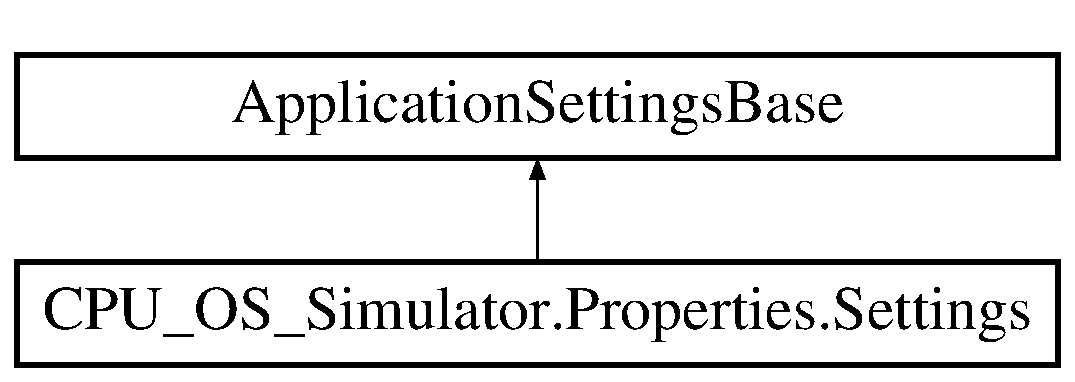
\includegraphics[height=2.000000cm]{class_c_p_u___o_s___simulator_1_1_properties_1_1_settings}
\end{center}
\end{figure}
\subsection*{Properties}
\begin{DoxyCompactItemize}
\item 
static \hyperlink{class_c_p_u___o_s___simulator_1_1_properties_1_1_settings}{Settings} \hyperlink{class_c_p_u___o_s___simulator_1_1_properties_1_1_settings_a423993327c18a4dfede5f73981018fca}{Default}\hspace{0.3cm}{\ttfamily  \mbox{[}get\mbox{]}}
\end{DoxyCompactItemize}
\subsection*{Static Private Attributes}
\begin{DoxyCompactItemize}
\item 
static \hyperlink{class_c_p_u___o_s___simulator_1_1_properties_1_1_settings}{Settings} \hyperlink{class_c_p_u___o_s___simulator_1_1_properties_1_1_settings_a9016562ea46f792bf8dc8d3e79dd36ae}{default\+Instance} = ((\hyperlink{class_c_p_u___o_s___simulator_1_1_properties_1_1_settings}{Settings})(Synchronized(new \hyperlink{class_c_p_u___o_s___simulator_1_1_properties_1_1_settings}{Settings}())))
\end{DoxyCompactItemize}


\subsection{Detailed Description}


Definition at line 20 of file Settings.\+Designer.\+cs.



\subsection{Member Data Documentation}
\hypertarget{class_c_p_u___o_s___simulator_1_1_properties_1_1_settings_a9016562ea46f792bf8dc8d3e79dd36ae}{}\index{C\+P\+U\+\_\+\+O\+S\+\_\+\+Simulator\+::\+Properties\+::\+Settings@{C\+P\+U\+\_\+\+O\+S\+\_\+\+Simulator\+::\+Properties\+::\+Settings}!default\+Instance@{default\+Instance}}
\index{default\+Instance@{default\+Instance}!C\+P\+U\+\_\+\+O\+S\+\_\+\+Simulator\+::\+Properties\+::\+Settings@{C\+P\+U\+\_\+\+O\+S\+\_\+\+Simulator\+::\+Properties\+::\+Settings}}
\subsubsection[{default\+Instance}]{\setlength{\rightskip}{0pt plus 5cm}{\bf Settings} C\+P\+U\+\_\+\+O\+S\+\_\+\+Simulator.\+Properties.\+Settings.\+default\+Instance = (({\bf Settings})(Synchronized(new {\bf Settings}())))\hspace{0.3cm}{\ttfamily [static]}, {\ttfamily [private]}}\label{class_c_p_u___o_s___simulator_1_1_properties_1_1_settings_a9016562ea46f792bf8dc8d3e79dd36ae}


Definition at line 22 of file Settings.\+Designer.\+cs.



\subsection{Property Documentation}
\hypertarget{class_c_p_u___o_s___simulator_1_1_properties_1_1_settings_a423993327c18a4dfede5f73981018fca}{}\index{C\+P\+U\+\_\+\+O\+S\+\_\+\+Simulator\+::\+Properties\+::\+Settings@{C\+P\+U\+\_\+\+O\+S\+\_\+\+Simulator\+::\+Properties\+::\+Settings}!Default@{Default}}
\index{Default@{Default}!C\+P\+U\+\_\+\+O\+S\+\_\+\+Simulator\+::\+Properties\+::\+Settings@{C\+P\+U\+\_\+\+O\+S\+\_\+\+Simulator\+::\+Properties\+::\+Settings}}
\subsubsection[{Default}]{\setlength{\rightskip}{0pt plus 5cm}{\bf Settings} C\+P\+U\+\_\+\+O\+S\+\_\+\+Simulator.\+Properties.\+Settings.\+Default\hspace{0.3cm}{\ttfamily [static]}, {\ttfamily [get]}}\label{class_c_p_u___o_s___simulator_1_1_properties_1_1_settings_a423993327c18a4dfede5f73981018fca}


Definition at line 24 of file Settings.\+Designer.\+cs.



The documentation for this class was generated from the following file\+:\begin{DoxyCompactItemize}
\item 
C\+P\+U-\/\+O\+S Simulator/\+Properties/\hyperlink{_c_p_u-_o_s_01_simulator_2_properties_2_settings_8_designer_8cs}{Settings.\+Designer.\+cs}\end{DoxyCompactItemize}

\hypertarget{class_c_p_u___o_s___simulator_1_1_c_p_u_1_1_simulator_program}{}\section{C\+P\+U\+\_\+\+O\+S\+\_\+\+Simulator.\+C\+P\+U.\+Simulator\+Program Class Reference}
\label{class_c_p_u___o_s___simulator_1_1_c_p_u_1_1_simulator_program}\index{C\+P\+U\+\_\+\+O\+S\+\_\+\+Simulator.\+C\+P\+U.\+Simulator\+Program@{C\+P\+U\+\_\+\+O\+S\+\_\+\+Simulator.\+C\+P\+U.\+Simulator\+Program}}


This class represents a program that can be run within the simulator  


\subsection*{Public Member Functions}
\begin{DoxyCompactItemize}
\item 
\hyperlink{class_c_p_u___o_s___simulator_1_1_c_p_u_1_1_simulator_program_a92873858cd0a0d7e506f5718788a9e5e}{Simulator\+Program} ()
\item 
\hyperlink{class_c_p_u___o_s___simulator_1_1_c_p_u_1_1_simulator_program_af30bc76187c64b374a48d6d7f9e94d54}{Simulator\+Program} (string \hyperlink{class_c_p_u___o_s___simulator_1_1_c_p_u_1_1_simulator_program_ad4797b5d81ceb01cd4207a97b7af36c5}{name}, Int32 \hyperlink{class_c_p_u___o_s___simulator_1_1_c_p_u_1_1_simulator_program_aaea4fb02fb8d22806ce58b957f9b573d}{base\+Address}, Int32 \hyperlink{class_c_p_u___o_s___simulator_1_1_c_p_u_1_1_simulator_program_ac4d19d17c7ee206ad6343884f3390054}{pages})
\begin{DoxyCompactList}\small\item\em Constructor for simulator program \end{DoxyCompactList}\item 
void \hyperlink{class_c_p_u___o_s___simulator_1_1_c_p_u_1_1_simulator_program_a6b6df3400e406b1dc6de3787f1a8fc61}{Add\+Instruction} (ref \hyperlink{class_c_p_u___o_s___simulator_1_1_c_p_u_1_1_instruction}{Instruction} ins)
\item 
void \hyperlink{class_c_p_u___o_s___simulator_1_1_c_p_u_1_1_simulator_program_a1142bf081f4173d0276504db3d232968}{Add\+Instruction} (ref \hyperlink{class_c_p_u___o_s___simulator_1_1_c_p_u_1_1_instruction}{Instruction} ins, int index)
\end{DoxyCompactItemize}
\subsection*{Properties}
\begin{DoxyCompactItemize}
\item 
string \hyperlink{class_c_p_u___o_s___simulator_1_1_c_p_u_1_1_simulator_program_a29b077a3403773010be9efe912d11b92}{Name}\hspace{0.3cm}{\ttfamily  \mbox{[}get, set\mbox{]}}
\begin{DoxyCompactList}\small\item\em Property for the name of the program \end{DoxyCompactList}\item 
int \hyperlink{class_c_p_u___o_s___simulator_1_1_c_p_u_1_1_simulator_program_ad07bee447d47fb07243a4484b5740c21}{Base\+Address}\hspace{0.3cm}{\ttfamily  \mbox{[}get, set\mbox{]}}
\begin{DoxyCompactList}\small\item\em Property for the base address of the program \end{DoxyCompactList}\item 
int \hyperlink{class_c_p_u___o_s___simulator_1_1_c_p_u_1_1_simulator_program_aa33b4428956a097dd710948ee51bb5f3}{Pages}\hspace{0.3cm}{\ttfamily  \mbox{[}get, set\mbox{]}}
\begin{DoxyCompactList}\small\item\em Property for the number of memory pages in the program \end{DoxyCompactList}\item 
List$<$ \hyperlink{class_c_p_u___o_s___simulator_1_1_c_p_u_1_1_instruction}{Instruction} $>$ \hyperlink{class_c_p_u___o_s___simulator_1_1_c_p_u_1_1_simulator_program_ae64c462081a1806d5f194c271dbb2686}{Instructions}\hspace{0.3cm}{\ttfamily  \mbox{[}get, set\mbox{]}}
\begin{DoxyCompactList}\small\item\em Property for the linked list of instructions that make up the program \end{DoxyCompactList}\item 
int \hyperlink{class_c_p_u___o_s___simulator_1_1_c_p_u_1_1_simulator_program_aeeb09200864db79b4a41f35cda644b87}{Start\+Address}\hspace{0.3cm}{\ttfamily  \mbox{[}get, set\mbox{]}}
\item 
List$<$ \hyperlink{class_c_p_u___o_s___simulator_1_1_memory_1_1_memory_page}{Memory\+Page} $>$ \hyperlink{class_c_p_u___o_s___simulator_1_1_c_p_u_1_1_simulator_program_ac3f520f751426a1e09f350096f0d2341}{Memory}\hspace{0.3cm}{\ttfamily  \mbox{[}get, set\mbox{]}}
\item 
\hyperlink{class_c_p_u___o_s___simulator_1_1_c_p_u_1_1_program_stack}{Program\+Stack} \hyperlink{class_c_p_u___o_s___simulator_1_1_c_p_u_1_1_simulator_program_ac6065e57e8d108a0aefd27840f3bf01c}{Stack}\hspace{0.3cm}{\ttfamily  \mbox{[}get, set\mbox{]}}
\end{DoxyCompactItemize}
\subsection*{Private Member Functions}
\begin{DoxyCompactItemize}
\item 
void \hyperlink{class_c_p_u___o_s___simulator_1_1_c_p_u_1_1_simulator_program_a4f7e933d4f3ca318d68471d465c6b31c}{Update\+Addresses} ()
\item 
int \hyperlink{class_c_p_u___o_s___simulator_1_1_c_p_u_1_1_simulator_program_a6ab84d4093d03fc387e4288dfc566388}{Calculate\+Address} (\hyperlink{class_c_p_u___o_s___simulator_1_1_c_p_u_1_1_instruction}{Instruction} instruction, int index)
\end{DoxyCompactItemize}
\subsection*{Private Attributes}
\begin{DoxyCompactItemize}
\item 
string \hyperlink{class_c_p_u___o_s___simulator_1_1_c_p_u_1_1_simulator_program_ad4797b5d81ceb01cd4207a97b7af36c5}{name}
\item 
Int32 \hyperlink{class_c_p_u___o_s___simulator_1_1_c_p_u_1_1_simulator_program_aaea4fb02fb8d22806ce58b957f9b573d}{base\+Address}
\item 
Int32 \hyperlink{class_c_p_u___o_s___simulator_1_1_c_p_u_1_1_simulator_program_a7b2581eff41da814292bf29936ab5318}{start\+Address}
\item 
Int32 \hyperlink{class_c_p_u___o_s___simulator_1_1_c_p_u_1_1_simulator_program_ac4d19d17c7ee206ad6343884f3390054}{pages}
\item 
\hyperlink{class_c_p_u___o_s___simulator_1_1_c_p_u_1_1_execution_unit}{Execution\+Unit} \hyperlink{class_c_p_u___o_s___simulator_1_1_c_p_u_1_1_simulator_program_a10e4c29c3ed9b84c0fb8aee7613cabf9}{unit}
\item 
List$<$ \hyperlink{class_c_p_u___o_s___simulator_1_1_c_p_u_1_1_instruction}{Instruction} $>$ \hyperlink{class_c_p_u___o_s___simulator_1_1_c_p_u_1_1_simulator_program_a30b501e0b2d012212077059be49857cf}{instructions}
\item 
List$<$ \hyperlink{class_c_p_u___o_s___simulator_1_1_memory_1_1_memory_page}{Memory\+Page} $>$ \hyperlink{class_c_p_u___o_s___simulator_1_1_c_p_u_1_1_simulator_program_a402e53ae5daf1b6be0d5b7b705091c9c}{memory}
\item 
\hyperlink{class_c_p_u___o_s___simulator_1_1_c_p_u_1_1_program_stack}{Program\+Stack} \hyperlink{class_c_p_u___o_s___simulator_1_1_c_p_u_1_1_simulator_program_a85f44af349486db4b141b3946bf21a64}{stack}
\end{DoxyCompactItemize}


\subsection{Detailed Description}
This class represents a program that can be run within the simulator 



Definition at line 12 of file Simulator\+Program.\+cs.



\subsection{Constructor \& Destructor Documentation}
\hypertarget{class_c_p_u___o_s___simulator_1_1_c_p_u_1_1_simulator_program_a92873858cd0a0d7e506f5718788a9e5e}{}\index{C\+P\+U\+\_\+\+O\+S\+\_\+\+Simulator\+::\+C\+P\+U\+::\+Simulator\+Program@{C\+P\+U\+\_\+\+O\+S\+\_\+\+Simulator\+::\+C\+P\+U\+::\+Simulator\+Program}!Simulator\+Program@{Simulator\+Program}}
\index{Simulator\+Program@{Simulator\+Program}!C\+P\+U\+\_\+\+O\+S\+\_\+\+Simulator\+::\+C\+P\+U\+::\+Simulator\+Program@{C\+P\+U\+\_\+\+O\+S\+\_\+\+Simulator\+::\+C\+P\+U\+::\+Simulator\+Program}}
\subsubsection[{Simulator\+Program()}]{\setlength{\rightskip}{0pt plus 5cm}C\+P\+U\+\_\+\+O\+S\+\_\+\+Simulator.\+C\+P\+U.\+Simulator\+Program.\+Simulator\+Program (
\begin{DoxyParamCaption}
{}
\end{DoxyParamCaption}
)}\label{class_c_p_u___o_s___simulator_1_1_c_p_u_1_1_simulator_program_a92873858cd0a0d7e506f5718788a9e5e}


Definition at line 33 of file Simulator\+Program.\+cs.

\hypertarget{class_c_p_u___o_s___simulator_1_1_c_p_u_1_1_simulator_program_af30bc76187c64b374a48d6d7f9e94d54}{}\index{C\+P\+U\+\_\+\+O\+S\+\_\+\+Simulator\+::\+C\+P\+U\+::\+Simulator\+Program@{C\+P\+U\+\_\+\+O\+S\+\_\+\+Simulator\+::\+C\+P\+U\+::\+Simulator\+Program}!Simulator\+Program@{Simulator\+Program}}
\index{Simulator\+Program@{Simulator\+Program}!C\+P\+U\+\_\+\+O\+S\+\_\+\+Simulator\+::\+C\+P\+U\+::\+Simulator\+Program@{C\+P\+U\+\_\+\+O\+S\+\_\+\+Simulator\+::\+C\+P\+U\+::\+Simulator\+Program}}
\subsubsection[{Simulator\+Program(string name, Int32 base\+Address, Int32 pages)}]{\setlength{\rightskip}{0pt plus 5cm}C\+P\+U\+\_\+\+O\+S\+\_\+\+Simulator.\+C\+P\+U.\+Simulator\+Program.\+Simulator\+Program (
\begin{DoxyParamCaption}
\item[{string}]{name, }
\item[{Int32}]{base\+Address, }
\item[{Int32}]{pages}
\end{DoxyParamCaption}
)}\label{class_c_p_u___o_s___simulator_1_1_c_p_u_1_1_simulator_program_af30bc76187c64b374a48d6d7f9e94d54}


Constructor for simulator program 


\begin{DoxyParams}{Parameters}
{\em name} & The name of the program\\
\hline
{\em base\+Address} & the base address of the program\\
\hline
{\em pages} & the number of memory pages in the program\\
\hline
\end{DoxyParams}


Definition at line 43 of file Simulator\+Program.\+cs.



\subsection{Member Function Documentation}
\hypertarget{class_c_p_u___o_s___simulator_1_1_c_p_u_1_1_simulator_program_a6b6df3400e406b1dc6de3787f1a8fc61}{}\index{C\+P\+U\+\_\+\+O\+S\+\_\+\+Simulator\+::\+C\+P\+U\+::\+Simulator\+Program@{C\+P\+U\+\_\+\+O\+S\+\_\+\+Simulator\+::\+C\+P\+U\+::\+Simulator\+Program}!Add\+Instruction@{Add\+Instruction}}
\index{Add\+Instruction@{Add\+Instruction}!C\+P\+U\+\_\+\+O\+S\+\_\+\+Simulator\+::\+C\+P\+U\+::\+Simulator\+Program@{C\+P\+U\+\_\+\+O\+S\+\_\+\+Simulator\+::\+C\+P\+U\+::\+Simulator\+Program}}
\subsubsection[{Add\+Instruction(ref Instruction ins)}]{\setlength{\rightskip}{0pt plus 5cm}void C\+P\+U\+\_\+\+O\+S\+\_\+\+Simulator.\+C\+P\+U.\+Simulator\+Program.\+Add\+Instruction (
\begin{DoxyParamCaption}
\item[{ref {\bf Instruction}}]{ins}
\end{DoxyParamCaption}
)}\label{class_c_p_u___o_s___simulator_1_1_c_p_u_1_1_simulator_program_a6b6df3400e406b1dc6de3787f1a8fc61}


Definition at line 168 of file Simulator\+Program.\+cs.

\hypertarget{class_c_p_u___o_s___simulator_1_1_c_p_u_1_1_simulator_program_a1142bf081f4173d0276504db3d232968}{}\index{C\+P\+U\+\_\+\+O\+S\+\_\+\+Simulator\+::\+C\+P\+U\+::\+Simulator\+Program@{C\+P\+U\+\_\+\+O\+S\+\_\+\+Simulator\+::\+C\+P\+U\+::\+Simulator\+Program}!Add\+Instruction@{Add\+Instruction}}
\index{Add\+Instruction@{Add\+Instruction}!C\+P\+U\+\_\+\+O\+S\+\_\+\+Simulator\+::\+C\+P\+U\+::\+Simulator\+Program@{C\+P\+U\+\_\+\+O\+S\+\_\+\+Simulator\+::\+C\+P\+U\+::\+Simulator\+Program}}
\subsubsection[{Add\+Instruction(ref Instruction ins, int index)}]{\setlength{\rightskip}{0pt plus 5cm}void C\+P\+U\+\_\+\+O\+S\+\_\+\+Simulator.\+C\+P\+U.\+Simulator\+Program.\+Add\+Instruction (
\begin{DoxyParamCaption}
\item[{ref {\bf Instruction}}]{ins, }
\item[{int}]{index}
\end{DoxyParamCaption}
)}\label{class_c_p_u___o_s___simulator_1_1_c_p_u_1_1_simulator_program_a1142bf081f4173d0276504db3d232968}


Definition at line 176 of file Simulator\+Program.\+cs.

\hypertarget{class_c_p_u___o_s___simulator_1_1_c_p_u_1_1_simulator_program_a6ab84d4093d03fc387e4288dfc566388}{}\index{C\+P\+U\+\_\+\+O\+S\+\_\+\+Simulator\+::\+C\+P\+U\+::\+Simulator\+Program@{C\+P\+U\+\_\+\+O\+S\+\_\+\+Simulator\+::\+C\+P\+U\+::\+Simulator\+Program}!Calculate\+Address@{Calculate\+Address}}
\index{Calculate\+Address@{Calculate\+Address}!C\+P\+U\+\_\+\+O\+S\+\_\+\+Simulator\+::\+C\+P\+U\+::\+Simulator\+Program@{C\+P\+U\+\_\+\+O\+S\+\_\+\+Simulator\+::\+C\+P\+U\+::\+Simulator\+Program}}
\subsubsection[{Calculate\+Address(\+Instruction instruction, int index)}]{\setlength{\rightskip}{0pt plus 5cm}int C\+P\+U\+\_\+\+O\+S\+\_\+\+Simulator.\+C\+P\+U.\+Simulator\+Program.\+Calculate\+Address (
\begin{DoxyParamCaption}
\item[{{\bf Instruction}}]{instruction, }
\item[{int}]{index}
\end{DoxyParamCaption}
)\hspace{0.3cm}{\ttfamily [private]}}\label{class_c_p_u___o_s___simulator_1_1_c_p_u_1_1_simulator_program_a6ab84d4093d03fc387e4288dfc566388}


Definition at line 196 of file Simulator\+Program.\+cs.

\hypertarget{class_c_p_u___o_s___simulator_1_1_c_p_u_1_1_simulator_program_a4f7e933d4f3ca318d68471d465c6b31c}{}\index{C\+P\+U\+\_\+\+O\+S\+\_\+\+Simulator\+::\+C\+P\+U\+::\+Simulator\+Program@{C\+P\+U\+\_\+\+O\+S\+\_\+\+Simulator\+::\+C\+P\+U\+::\+Simulator\+Program}!Update\+Addresses@{Update\+Addresses}}
\index{Update\+Addresses@{Update\+Addresses}!C\+P\+U\+\_\+\+O\+S\+\_\+\+Simulator\+::\+C\+P\+U\+::\+Simulator\+Program@{C\+P\+U\+\_\+\+O\+S\+\_\+\+Simulator\+::\+C\+P\+U\+::\+Simulator\+Program}}
\subsubsection[{Update\+Addresses()}]{\setlength{\rightskip}{0pt plus 5cm}void C\+P\+U\+\_\+\+O\+S\+\_\+\+Simulator.\+C\+P\+U.\+Simulator\+Program.\+Update\+Addresses (
\begin{DoxyParamCaption}
{}
\end{DoxyParamCaption}
)\hspace{0.3cm}{\ttfamily [private]}}\label{class_c_p_u___o_s___simulator_1_1_c_p_u_1_1_simulator_program_a4f7e933d4f3ca318d68471d465c6b31c}


Definition at line 184 of file Simulator\+Program.\+cs.



\subsection{Member Data Documentation}
\hypertarget{class_c_p_u___o_s___simulator_1_1_c_p_u_1_1_simulator_program_aaea4fb02fb8d22806ce58b957f9b573d}{}\index{C\+P\+U\+\_\+\+O\+S\+\_\+\+Simulator\+::\+C\+P\+U\+::\+Simulator\+Program@{C\+P\+U\+\_\+\+O\+S\+\_\+\+Simulator\+::\+C\+P\+U\+::\+Simulator\+Program}!base\+Address@{base\+Address}}
\index{base\+Address@{base\+Address}!C\+P\+U\+\_\+\+O\+S\+\_\+\+Simulator\+::\+C\+P\+U\+::\+Simulator\+Program@{C\+P\+U\+\_\+\+O\+S\+\_\+\+Simulator\+::\+C\+P\+U\+::\+Simulator\+Program}}
\subsubsection[{base\+Address}]{\setlength{\rightskip}{0pt plus 5cm}Int32 C\+P\+U\+\_\+\+O\+S\+\_\+\+Simulator.\+C\+P\+U.\+Simulator\+Program.\+base\+Address\hspace{0.3cm}{\ttfamily [private]}}\label{class_c_p_u___o_s___simulator_1_1_c_p_u_1_1_simulator_program_aaea4fb02fb8d22806ce58b957f9b573d}


Definition at line 17 of file Simulator\+Program.\+cs.

\hypertarget{class_c_p_u___o_s___simulator_1_1_c_p_u_1_1_simulator_program_a30b501e0b2d012212077059be49857cf}{}\index{C\+P\+U\+\_\+\+O\+S\+\_\+\+Simulator\+::\+C\+P\+U\+::\+Simulator\+Program@{C\+P\+U\+\_\+\+O\+S\+\_\+\+Simulator\+::\+C\+P\+U\+::\+Simulator\+Program}!instructions@{instructions}}
\index{instructions@{instructions}!C\+P\+U\+\_\+\+O\+S\+\_\+\+Simulator\+::\+C\+P\+U\+::\+Simulator\+Program@{C\+P\+U\+\_\+\+O\+S\+\_\+\+Simulator\+::\+C\+P\+U\+::\+Simulator\+Program}}
\subsubsection[{instructions}]{\setlength{\rightskip}{0pt plus 5cm}List$<${\bf Instruction}$>$ C\+P\+U\+\_\+\+O\+S\+\_\+\+Simulator.\+C\+P\+U.\+Simulator\+Program.\+instructions\hspace{0.3cm}{\ttfamily [private]}}\label{class_c_p_u___o_s___simulator_1_1_c_p_u_1_1_simulator_program_a30b501e0b2d012212077059be49857cf}


Definition at line 21 of file Simulator\+Program.\+cs.

\hypertarget{class_c_p_u___o_s___simulator_1_1_c_p_u_1_1_simulator_program_a402e53ae5daf1b6be0d5b7b705091c9c}{}\index{C\+P\+U\+\_\+\+O\+S\+\_\+\+Simulator\+::\+C\+P\+U\+::\+Simulator\+Program@{C\+P\+U\+\_\+\+O\+S\+\_\+\+Simulator\+::\+C\+P\+U\+::\+Simulator\+Program}!memory@{memory}}
\index{memory@{memory}!C\+P\+U\+\_\+\+O\+S\+\_\+\+Simulator\+::\+C\+P\+U\+::\+Simulator\+Program@{C\+P\+U\+\_\+\+O\+S\+\_\+\+Simulator\+::\+C\+P\+U\+::\+Simulator\+Program}}
\subsubsection[{memory}]{\setlength{\rightskip}{0pt plus 5cm}List$<${\bf Memory\+Page}$>$ C\+P\+U\+\_\+\+O\+S\+\_\+\+Simulator.\+C\+P\+U.\+Simulator\+Program.\+memory\hspace{0.3cm}{\ttfamily [private]}}\label{class_c_p_u___o_s___simulator_1_1_c_p_u_1_1_simulator_program_a402e53ae5daf1b6be0d5b7b705091c9c}


Definition at line 24 of file Simulator\+Program.\+cs.

\hypertarget{class_c_p_u___o_s___simulator_1_1_c_p_u_1_1_simulator_program_ad4797b5d81ceb01cd4207a97b7af36c5}{}\index{C\+P\+U\+\_\+\+O\+S\+\_\+\+Simulator\+::\+C\+P\+U\+::\+Simulator\+Program@{C\+P\+U\+\_\+\+O\+S\+\_\+\+Simulator\+::\+C\+P\+U\+::\+Simulator\+Program}!name@{name}}
\index{name@{name}!C\+P\+U\+\_\+\+O\+S\+\_\+\+Simulator\+::\+C\+P\+U\+::\+Simulator\+Program@{C\+P\+U\+\_\+\+O\+S\+\_\+\+Simulator\+::\+C\+P\+U\+::\+Simulator\+Program}}
\subsubsection[{name}]{\setlength{\rightskip}{0pt plus 5cm}string C\+P\+U\+\_\+\+O\+S\+\_\+\+Simulator.\+C\+P\+U.\+Simulator\+Program.\+name\hspace{0.3cm}{\ttfamily [private]}}\label{class_c_p_u___o_s___simulator_1_1_c_p_u_1_1_simulator_program_ad4797b5d81ceb01cd4207a97b7af36c5}


Definition at line 16 of file Simulator\+Program.\+cs.

\hypertarget{class_c_p_u___o_s___simulator_1_1_c_p_u_1_1_simulator_program_ac4d19d17c7ee206ad6343884f3390054}{}\index{C\+P\+U\+\_\+\+O\+S\+\_\+\+Simulator\+::\+C\+P\+U\+::\+Simulator\+Program@{C\+P\+U\+\_\+\+O\+S\+\_\+\+Simulator\+::\+C\+P\+U\+::\+Simulator\+Program}!pages@{pages}}
\index{pages@{pages}!C\+P\+U\+\_\+\+O\+S\+\_\+\+Simulator\+::\+C\+P\+U\+::\+Simulator\+Program@{C\+P\+U\+\_\+\+O\+S\+\_\+\+Simulator\+::\+C\+P\+U\+::\+Simulator\+Program}}
\subsubsection[{pages}]{\setlength{\rightskip}{0pt plus 5cm}Int32 C\+P\+U\+\_\+\+O\+S\+\_\+\+Simulator.\+C\+P\+U.\+Simulator\+Program.\+pages\hspace{0.3cm}{\ttfamily [private]}}\label{class_c_p_u___o_s___simulator_1_1_c_p_u_1_1_simulator_program_ac4d19d17c7ee206ad6343884f3390054}


Definition at line 19 of file Simulator\+Program.\+cs.

\hypertarget{class_c_p_u___o_s___simulator_1_1_c_p_u_1_1_simulator_program_a85f44af349486db4b141b3946bf21a64}{}\index{C\+P\+U\+\_\+\+O\+S\+\_\+\+Simulator\+::\+C\+P\+U\+::\+Simulator\+Program@{C\+P\+U\+\_\+\+O\+S\+\_\+\+Simulator\+::\+C\+P\+U\+::\+Simulator\+Program}!stack@{stack}}
\index{stack@{stack}!C\+P\+U\+\_\+\+O\+S\+\_\+\+Simulator\+::\+C\+P\+U\+::\+Simulator\+Program@{C\+P\+U\+\_\+\+O\+S\+\_\+\+Simulator\+::\+C\+P\+U\+::\+Simulator\+Program}}
\subsubsection[{stack}]{\setlength{\rightskip}{0pt plus 5cm}{\bf Program\+Stack} C\+P\+U\+\_\+\+O\+S\+\_\+\+Simulator.\+C\+P\+U.\+Simulator\+Program.\+stack\hspace{0.3cm}{\ttfamily [private]}}\label{class_c_p_u___o_s___simulator_1_1_c_p_u_1_1_simulator_program_a85f44af349486db4b141b3946bf21a64}


Definition at line 27 of file Simulator\+Program.\+cs.

\hypertarget{class_c_p_u___o_s___simulator_1_1_c_p_u_1_1_simulator_program_a7b2581eff41da814292bf29936ab5318}{}\index{C\+P\+U\+\_\+\+O\+S\+\_\+\+Simulator\+::\+C\+P\+U\+::\+Simulator\+Program@{C\+P\+U\+\_\+\+O\+S\+\_\+\+Simulator\+::\+C\+P\+U\+::\+Simulator\+Program}!start\+Address@{start\+Address}}
\index{start\+Address@{start\+Address}!C\+P\+U\+\_\+\+O\+S\+\_\+\+Simulator\+::\+C\+P\+U\+::\+Simulator\+Program@{C\+P\+U\+\_\+\+O\+S\+\_\+\+Simulator\+::\+C\+P\+U\+::\+Simulator\+Program}}
\subsubsection[{start\+Address}]{\setlength{\rightskip}{0pt plus 5cm}Int32 C\+P\+U\+\_\+\+O\+S\+\_\+\+Simulator.\+C\+P\+U.\+Simulator\+Program.\+start\+Address\hspace{0.3cm}{\ttfamily [private]}}\label{class_c_p_u___o_s___simulator_1_1_c_p_u_1_1_simulator_program_a7b2581eff41da814292bf29936ab5318}


Definition at line 18 of file Simulator\+Program.\+cs.

\hypertarget{class_c_p_u___o_s___simulator_1_1_c_p_u_1_1_simulator_program_a10e4c29c3ed9b84c0fb8aee7613cabf9}{}\index{C\+P\+U\+\_\+\+O\+S\+\_\+\+Simulator\+::\+C\+P\+U\+::\+Simulator\+Program@{C\+P\+U\+\_\+\+O\+S\+\_\+\+Simulator\+::\+C\+P\+U\+::\+Simulator\+Program}!unit@{unit}}
\index{unit@{unit}!C\+P\+U\+\_\+\+O\+S\+\_\+\+Simulator\+::\+C\+P\+U\+::\+Simulator\+Program@{C\+P\+U\+\_\+\+O\+S\+\_\+\+Simulator\+::\+C\+P\+U\+::\+Simulator\+Program}}
\subsubsection[{unit}]{\setlength{\rightskip}{0pt plus 5cm}{\bf Execution\+Unit} C\+P\+U\+\_\+\+O\+S\+\_\+\+Simulator.\+C\+P\+U.\+Simulator\+Program.\+unit\hspace{0.3cm}{\ttfamily [private]}}\label{class_c_p_u___o_s___simulator_1_1_c_p_u_1_1_simulator_program_a10e4c29c3ed9b84c0fb8aee7613cabf9}


Definition at line 20 of file Simulator\+Program.\+cs.



\subsection{Property Documentation}
\hypertarget{class_c_p_u___o_s___simulator_1_1_c_p_u_1_1_simulator_program_ad07bee447d47fb07243a4484b5740c21}{}\index{C\+P\+U\+\_\+\+O\+S\+\_\+\+Simulator\+::\+C\+P\+U\+::\+Simulator\+Program@{C\+P\+U\+\_\+\+O\+S\+\_\+\+Simulator\+::\+C\+P\+U\+::\+Simulator\+Program}!Base\+Address@{Base\+Address}}
\index{Base\+Address@{Base\+Address}!C\+P\+U\+\_\+\+O\+S\+\_\+\+Simulator\+::\+C\+P\+U\+::\+Simulator\+Program@{C\+P\+U\+\_\+\+O\+S\+\_\+\+Simulator\+::\+C\+P\+U\+::\+Simulator\+Program}}
\subsubsection[{Base\+Address}]{\setlength{\rightskip}{0pt plus 5cm}int C\+P\+U\+\_\+\+O\+S\+\_\+\+Simulator.\+C\+P\+U.\+Simulator\+Program.\+Base\+Address\hspace{0.3cm}{\ttfamily [get]}, {\ttfamily [set]}}\label{class_c_p_u___o_s___simulator_1_1_c_p_u_1_1_simulator_program_ad07bee447d47fb07243a4484b5740c21}


Property for the base address of the program 



Definition at line 79 of file Simulator\+Program.\+cs.

\hypertarget{class_c_p_u___o_s___simulator_1_1_c_p_u_1_1_simulator_program_ae64c462081a1806d5f194c271dbb2686}{}\index{C\+P\+U\+\_\+\+O\+S\+\_\+\+Simulator\+::\+C\+P\+U\+::\+Simulator\+Program@{C\+P\+U\+\_\+\+O\+S\+\_\+\+Simulator\+::\+C\+P\+U\+::\+Simulator\+Program}!Instructions@{Instructions}}
\index{Instructions@{Instructions}!C\+P\+U\+\_\+\+O\+S\+\_\+\+Simulator\+::\+C\+P\+U\+::\+Simulator\+Program@{C\+P\+U\+\_\+\+O\+S\+\_\+\+Simulator\+::\+C\+P\+U\+::\+Simulator\+Program}}
\subsubsection[{Instructions}]{\setlength{\rightskip}{0pt plus 5cm}List$<${\bf Instruction}$>$ C\+P\+U\+\_\+\+O\+S\+\_\+\+Simulator.\+C\+P\+U.\+Simulator\+Program.\+Instructions\hspace{0.3cm}{\ttfamily [get]}, {\ttfamily [set]}}\label{class_c_p_u___o_s___simulator_1_1_c_p_u_1_1_simulator_program_ae64c462081a1806d5f194c271dbb2686}


Property for the linked list of instructions that make up the program 



Definition at line 111 of file Simulator\+Program.\+cs.

\hypertarget{class_c_p_u___o_s___simulator_1_1_c_p_u_1_1_simulator_program_ac3f520f751426a1e09f350096f0d2341}{}\index{C\+P\+U\+\_\+\+O\+S\+\_\+\+Simulator\+::\+C\+P\+U\+::\+Simulator\+Program@{C\+P\+U\+\_\+\+O\+S\+\_\+\+Simulator\+::\+C\+P\+U\+::\+Simulator\+Program}!Memory@{Memory}}
\index{Memory@{Memory}!C\+P\+U\+\_\+\+O\+S\+\_\+\+Simulator\+::\+C\+P\+U\+::\+Simulator\+Program@{C\+P\+U\+\_\+\+O\+S\+\_\+\+Simulator\+::\+C\+P\+U\+::\+Simulator\+Program}}
\subsubsection[{Memory}]{\setlength{\rightskip}{0pt plus 5cm}List$<${\bf Memory\+Page}$>$ C\+P\+U\+\_\+\+O\+S\+\_\+\+Simulator.\+C\+P\+U.\+Simulator\+Program.\+Memory\hspace{0.3cm}{\ttfamily [get]}, {\ttfamily [set]}}\label{class_c_p_u___o_s___simulator_1_1_c_p_u_1_1_simulator_program_ac3f520f751426a1e09f350096f0d2341}


Definition at line 138 of file Simulator\+Program.\+cs.

\hypertarget{class_c_p_u___o_s___simulator_1_1_c_p_u_1_1_simulator_program_a29b077a3403773010be9efe912d11b92}{}\index{C\+P\+U\+\_\+\+O\+S\+\_\+\+Simulator\+::\+C\+P\+U\+::\+Simulator\+Program@{C\+P\+U\+\_\+\+O\+S\+\_\+\+Simulator\+::\+C\+P\+U\+::\+Simulator\+Program}!Name@{Name}}
\index{Name@{Name}!C\+P\+U\+\_\+\+O\+S\+\_\+\+Simulator\+::\+C\+P\+U\+::\+Simulator\+Program@{C\+P\+U\+\_\+\+O\+S\+\_\+\+Simulator\+::\+C\+P\+U\+::\+Simulator\+Program}}
\subsubsection[{Name}]{\setlength{\rightskip}{0pt plus 5cm}string C\+P\+U\+\_\+\+O\+S\+\_\+\+Simulator.\+C\+P\+U.\+Simulator\+Program.\+Name\hspace{0.3cm}{\ttfamily [get]}, {\ttfamily [set]}}\label{class_c_p_u___o_s___simulator_1_1_c_p_u_1_1_simulator_program_a29b077a3403773010be9efe912d11b92}


Property for the name of the program 



Definition at line 63 of file Simulator\+Program.\+cs.

\hypertarget{class_c_p_u___o_s___simulator_1_1_c_p_u_1_1_simulator_program_aa33b4428956a097dd710948ee51bb5f3}{}\index{C\+P\+U\+\_\+\+O\+S\+\_\+\+Simulator\+::\+C\+P\+U\+::\+Simulator\+Program@{C\+P\+U\+\_\+\+O\+S\+\_\+\+Simulator\+::\+C\+P\+U\+::\+Simulator\+Program}!Pages@{Pages}}
\index{Pages@{Pages}!C\+P\+U\+\_\+\+O\+S\+\_\+\+Simulator\+::\+C\+P\+U\+::\+Simulator\+Program@{C\+P\+U\+\_\+\+O\+S\+\_\+\+Simulator\+::\+C\+P\+U\+::\+Simulator\+Program}}
\subsubsection[{Pages}]{\setlength{\rightskip}{0pt plus 5cm}int C\+P\+U\+\_\+\+O\+S\+\_\+\+Simulator.\+C\+P\+U.\+Simulator\+Program.\+Pages\hspace{0.3cm}{\ttfamily [get]}, {\ttfamily [set]}}\label{class_c_p_u___o_s___simulator_1_1_c_p_u_1_1_simulator_program_aa33b4428956a097dd710948ee51bb5f3}


Property for the number of memory pages in the program 



Definition at line 95 of file Simulator\+Program.\+cs.

\hypertarget{class_c_p_u___o_s___simulator_1_1_c_p_u_1_1_simulator_program_ac6065e57e8d108a0aefd27840f3bf01c}{}\index{C\+P\+U\+\_\+\+O\+S\+\_\+\+Simulator\+::\+C\+P\+U\+::\+Simulator\+Program@{C\+P\+U\+\_\+\+O\+S\+\_\+\+Simulator\+::\+C\+P\+U\+::\+Simulator\+Program}!Stack@{Stack}}
\index{Stack@{Stack}!C\+P\+U\+\_\+\+O\+S\+\_\+\+Simulator\+::\+C\+P\+U\+::\+Simulator\+Program@{C\+P\+U\+\_\+\+O\+S\+\_\+\+Simulator\+::\+C\+P\+U\+::\+Simulator\+Program}}
\subsubsection[{Stack}]{\setlength{\rightskip}{0pt plus 5cm}{\bf Program\+Stack} C\+P\+U\+\_\+\+O\+S\+\_\+\+Simulator.\+C\+P\+U.\+Simulator\+Program.\+Stack\hspace{0.3cm}{\ttfamily [get]}, {\ttfamily [set]}}\label{class_c_p_u___o_s___simulator_1_1_c_p_u_1_1_simulator_program_ac6065e57e8d108a0aefd27840f3bf01c}


Definition at line 152 of file Simulator\+Program.\+cs.

\hypertarget{class_c_p_u___o_s___simulator_1_1_c_p_u_1_1_simulator_program_aeeb09200864db79b4a41f35cda644b87}{}\index{C\+P\+U\+\_\+\+O\+S\+\_\+\+Simulator\+::\+C\+P\+U\+::\+Simulator\+Program@{C\+P\+U\+\_\+\+O\+S\+\_\+\+Simulator\+::\+C\+P\+U\+::\+Simulator\+Program}!Start\+Address@{Start\+Address}}
\index{Start\+Address@{Start\+Address}!C\+P\+U\+\_\+\+O\+S\+\_\+\+Simulator\+::\+C\+P\+U\+::\+Simulator\+Program@{C\+P\+U\+\_\+\+O\+S\+\_\+\+Simulator\+::\+C\+P\+U\+::\+Simulator\+Program}}
\subsubsection[{Start\+Address}]{\setlength{\rightskip}{0pt plus 5cm}int C\+P\+U\+\_\+\+O\+S\+\_\+\+Simulator.\+C\+P\+U.\+Simulator\+Program.\+Start\+Address\hspace{0.3cm}{\ttfamily [get]}, {\ttfamily [set]}}\label{class_c_p_u___o_s___simulator_1_1_c_p_u_1_1_simulator_program_aeeb09200864db79b4a41f35cda644b87}


Definition at line 124 of file Simulator\+Program.\+cs.



The documentation for this class was generated from the following file\+:\begin{DoxyCompactItemize}
\item 
C\+P\+U/\hyperlink{_simulator_program_8cs}{Simulator\+Program.\+cs}\end{DoxyCompactItemize}

\hypertarget{class_c_p_u___o_s___simulator_1_1_c_p_u_1_1_special_register}{}\section{C\+P\+U\+\_\+\+O\+S\+\_\+\+Simulator.\+C\+P\+U.\+Special\+Register Class Reference}
\label{class_c_p_u___o_s___simulator_1_1_c_p_u_1_1_special_register}\index{C\+P\+U\+\_\+\+O\+S\+\_\+\+Simulator.\+C\+P\+U.\+Special\+Register@{C\+P\+U\+\_\+\+O\+S\+\_\+\+Simulator.\+C\+P\+U.\+Special\+Register}}


This class represents a special register i.\+e a non general purpose register  


Inheritance diagram for C\+P\+U\+\_\+\+O\+S\+\_\+\+Simulator.\+C\+P\+U.\+Special\+Register\+:\begin{figure}[H]
\begin{center}
\leavevmode
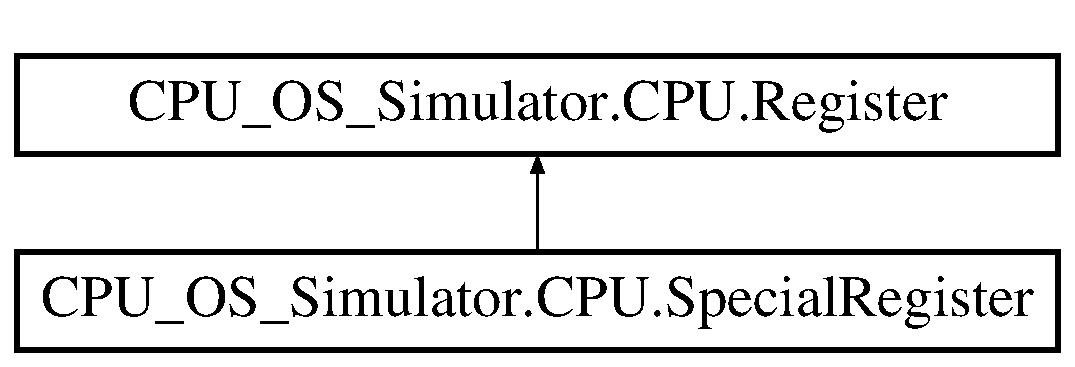
\includegraphics[height=2.000000cm]{class_c_p_u___o_s___simulator_1_1_c_p_u_1_1_special_register}
\end{center}
\end{figure}
\subsection*{Public Member Functions}
\begin{DoxyCompactItemize}
\item 
\hyperlink{class_c_p_u___o_s___simulator_1_1_c_p_u_1_1_special_register_a697f3e6f938ad7ab0ceee0555fe2c312}{Special\+Register} ()
\item 
void \hyperlink{class_c_p_u___o_s___simulator_1_1_c_p_u_1_1_special_register_ab76c9ab94069230fdf14821495ac9e9c}{set\+Register\+Value} (int \hyperlink{class_c_p_u___o_s___simulator_1_1_c_p_u_1_1_special_register_a040dbed0c42c3a45ccb7b01d181dd829}{value}, \hyperlink{namespace_c_p_u___o_s___simulator_1_1_c_p_u_ad49cfe442b74115a326c03b7ae848f76}{Enum\+Operand\+Type} \hyperlink{class_c_p_u___o_s___simulator_1_1_c_p_u_1_1_special_register_aae2bca6c1354013cca156bd19c30640d}{type})
\begin{DoxyCompactList}\small\item\em Sets the value in a special register \end{DoxyCompactList}\item 
void \hyperlink{class_c_p_u___o_s___simulator_1_1_c_p_u_1_1_special_register_a6c2605883e6349c10e92f5453c2ad9ea}{set\+Register\+Value} (string \hyperlink{class_c_p_u___o_s___simulator_1_1_c_p_u_1_1_special_register_a040dbed0c42c3a45ccb7b01d181dd829}{value}, \hyperlink{namespace_c_p_u___o_s___simulator_1_1_c_p_u_ad49cfe442b74115a326c03b7ae848f76}{Enum\+Operand\+Type} \hyperlink{class_c_p_u___o_s___simulator_1_1_c_p_u_1_1_special_register_aae2bca6c1354013cca156bd19c30640d}{type})
\begin{DoxyCompactList}\small\item\em Sets the string value in a special register \end{DoxyCompactList}\end{DoxyCompactItemize}
\subsection*{Static Public Member Functions}
\begin{DoxyCompactItemize}
\item 
static \hyperlink{class_c_p_u___o_s___simulator_1_1_c_p_u_1_1_special_register}{Special\+Register} \hyperlink{class_c_p_u___o_s___simulator_1_1_c_p_u_1_1_special_register_aa8c2e88c7311076eb6fd42ecb5d64e38}{Find\+Special\+Register} (string \hyperlink{class_c_p_u___o_s___simulator_1_1_c_p_u_1_1_special_register_ac521aef66f5fe6a88486e70f5ade8326}{name})
\end{DoxyCompactItemize}
\subsection*{Static Public Attributes}
\begin{DoxyCompactItemize}
\item 
static \hyperlink{class_c_p_u___o_s___simulator_1_1_c_p_u_1_1_special_register}{Special\+Register} \hyperlink{class_c_p_u___o_s___simulator_1_1_c_p_u_1_1_special_register_afc3205003157a5f135752e6a4f8ffb8a}{P\+C} = new \hyperlink{class_c_p_u___o_s___simulator_1_1_c_p_u_1_1_special_register}{Special\+Register}(\char`\"{}P\+C\char`\"{})
\begin{DoxyCompactList}\small\item\em The Program Counter register \end{DoxyCompactList}\item 
static \hyperlink{class_c_p_u___o_s___simulator_1_1_c_p_u_1_1_special_register}{Special\+Register} \hyperlink{class_c_p_u___o_s___simulator_1_1_c_p_u_1_1_special_register_a556243e1c3c891e685bf884771c1575c}{S\+R} = new \hyperlink{class_c_p_u___o_s___simulator_1_1_c_p_u_1_1_special_register}{Special\+Register}(\char`\"{}S\+R\char`\"{})
\begin{DoxyCompactList}\small\item\em The Stack \hyperlink{class_c_p_u___o_s___simulator_1_1_c_p_u_1_1_register}{Register} \end{DoxyCompactList}\item 
static \hyperlink{class_c_p_u___o_s___simulator_1_1_c_p_u_1_1_special_register}{Special\+Register} \hyperlink{class_c_p_u___o_s___simulator_1_1_c_p_u_1_1_special_register_ae1699c7972763e73e3f1cfe467cc82e9}{S\+P} = new \hyperlink{class_c_p_u___o_s___simulator_1_1_c_p_u_1_1_special_register}{Special\+Register}(\char`\"{}S\+P\char`\"{})
\begin{DoxyCompactList}\small\item\em The Stack Pointer \hyperlink{class_c_p_u___o_s___simulator_1_1_c_p_u_1_1_register}{Register} \end{DoxyCompactList}\item 
static \hyperlink{class_c_p_u___o_s___simulator_1_1_c_p_u_1_1_special_register}{Special\+Register} \hyperlink{class_c_p_u___o_s___simulator_1_1_c_p_u_1_1_special_register_a08c44f677cc5e830000382725ce8ab9f}{B\+R} = new \hyperlink{class_c_p_u___o_s___simulator_1_1_c_p_u_1_1_special_register}{Special\+Register}(\char`\"{}B\+R\char`\"{})
\item 
static \hyperlink{class_c_p_u___o_s___simulator_1_1_c_p_u_1_1_special_register}{Special\+Register} \hyperlink{class_c_p_u___o_s___simulator_1_1_c_p_u_1_1_special_register_a96fde61578e06f00ab7b19a4b05b9885}{I\+R} = new \hyperlink{class_c_p_u___o_s___simulator_1_1_c_p_u_1_1_special_register}{Special\+Register}(\char`\"{}I\+R\char`\"{})
\begin{DoxyCompactList}\small\item\em The \hyperlink{class_c_p_u___o_s___simulator_1_1_c_p_u_1_1_instruction}{Instruction} \hyperlink{class_c_p_u___o_s___simulator_1_1_c_p_u_1_1_register}{Register} \end{DoxyCompactList}\item 
static \hyperlink{class_c_p_u___o_s___simulator_1_1_c_p_u_1_1_special_register}{Special\+Register} \hyperlink{class_c_p_u___o_s___simulator_1_1_c_p_u_1_1_special_register_aabf7c761e1f8a9994b7c0b131c53924d}{M\+D\+R} = new \hyperlink{class_c_p_u___o_s___simulator_1_1_c_p_u_1_1_special_register}{Special\+Register}(\char`\"{}M\+D\+R\char`\"{})
\begin{DoxyCompactList}\small\item\em The \hyperlink{namespace_c_p_u___o_s___simulator_1_1_memory}{Memory} Data \hyperlink{class_c_p_u___o_s___simulator_1_1_c_p_u_1_1_register}{Register} \end{DoxyCompactList}\item 
static \hyperlink{class_c_p_u___o_s___simulator_1_1_c_p_u_1_1_special_register}{Special\+Register} \hyperlink{class_c_p_u___o_s___simulator_1_1_c_p_u_1_1_special_register_a2ae89cee8b74f9985f43ee4e6f994bad}{M\+A\+R} = new \hyperlink{class_c_p_u___o_s___simulator_1_1_c_p_u_1_1_special_register}{Special\+Register}(\char`\"{}M\+A\+R\char`\"{})
\begin{DoxyCompactList}\small\item\em The \hyperlink{namespace_c_p_u___o_s___simulator_1_1_memory}{Memory} Logical\+Address \hyperlink{class_c_p_u___o_s___simulator_1_1_c_p_u_1_1_register}{Register} \end{DoxyCompactList}\end{DoxyCompactItemize}
\subsection*{Protected Member Functions}
\begin{DoxyCompactItemize}
\item 
\hyperlink{class_c_p_u___o_s___simulator_1_1_c_p_u_1_1_special_register_a0328b3388027aa409a68191685753f4a}{Special\+Register} (string \hyperlink{class_c_p_u___o_s___simulator_1_1_c_p_u_1_1_special_register_ac521aef66f5fe6a88486e70f5ade8326}{name})
\begin{DoxyCompactList}\small\item\em Primary constructor for a special register \end{DoxyCompactList}\end{DoxyCompactItemize}
\subsection*{Properties}
\begin{DoxyCompactItemize}
\item 
string \hyperlink{class_c_p_u___o_s___simulator_1_1_c_p_u_1_1_special_register_ad8ad1efaf680db5471184a74f911b558}{Name}\hspace{0.3cm}{\ttfamily  \mbox{[}get, set\mbox{]}}
\begin{DoxyCompactList}\small\item\em Property for the name of the special register \end{DoxyCompactList}\item 
int \hyperlink{class_c_p_u___o_s___simulator_1_1_c_p_u_1_1_special_register_aeff33618d376eeaef1e62d6833074bd4}{Value}\hspace{0.3cm}{\ttfamily  \mbox{[}get, set\mbox{]}}
\begin{DoxyCompactList}\small\item\em Property for the value stored in the special register \end{DoxyCompactList}\item 
\hyperlink{namespace_c_p_u___o_s___simulator_1_1_c_p_u_ad49cfe442b74115a326c03b7ae848f76}{Enum\+Operand\+Type} \hyperlink{class_c_p_u___o_s___simulator_1_1_c_p_u_1_1_special_register_afd9e45080d792861e577dde31cdb6d3e}{Type}\hspace{0.3cm}{\ttfamily  \mbox{[}get, set\mbox{]}}
\begin{DoxyCompactList}\small\item\em Property for the type of data in the special register i.\+e. Value or \hyperlink{namespace_c_p_u___o_s___simulator_1_1_memory}{Memory} Address \end{DoxyCompactList}\item 
string \hyperlink{class_c_p_u___o_s___simulator_1_1_c_p_u_1_1_special_register_a60a2bcd516cedf8bb485c2e36bbc3235}{Value\+String}\hspace{0.3cm}{\ttfamily  \mbox{[}get, set\mbox{]}}
\begin{DoxyCompactList}\small\item\em Property for the value stored in the special register \end{DoxyCompactList}\end{DoxyCompactItemize}
\subsection*{Static Private Member Functions}
\begin{DoxyCompactItemize}
\item 
static dynamic \hyperlink{class_c_p_u___o_s___simulator_1_1_c_p_u_1_1_special_register_a0ed54c8fcd7674bcb87fef3eda712af2}{Get\+Main\+Window\+Instance} ()
\begin{DoxyCompactList}\small\item\em This function gets the main window instance from the window bridge \end{DoxyCompactList}\end{DoxyCompactItemize}
\subsection*{Private Attributes}
\begin{DoxyCompactItemize}
\item 
string \hyperlink{class_c_p_u___o_s___simulator_1_1_c_p_u_1_1_special_register_ac521aef66f5fe6a88486e70f5ade8326}{name}
\begin{DoxyCompactList}\small\item\em The name of the Special \hyperlink{class_c_p_u___o_s___simulator_1_1_c_p_u_1_1_register}{Register} \end{DoxyCompactList}\item 
int \hyperlink{class_c_p_u___o_s___simulator_1_1_c_p_u_1_1_special_register_a040dbed0c42c3a45ccb7b01d181dd829}{value}
\begin{DoxyCompactList}\small\item\em The integer value of the special register \end{DoxyCompactList}\item 
string \hyperlink{class_c_p_u___o_s___simulator_1_1_c_p_u_1_1_special_register_a540a55b17a53591312e76689d051abac}{value\+String}
\item 
\hyperlink{namespace_c_p_u___o_s___simulator_1_1_c_p_u_ad49cfe442b74115a326c03b7ae848f76}{Enum\+Operand\+Type} \hyperlink{class_c_p_u___o_s___simulator_1_1_c_p_u_1_1_special_register_aae2bca6c1354013cca156bd19c30640d}{type}
\end{DoxyCompactItemize}


\subsection{Detailed Description}
This class represents a special register i.\+e a non general purpose register 



Definition at line 10 of file Special\+Register.\+cs.



\subsection{Constructor \& Destructor Documentation}
\hypertarget{class_c_p_u___o_s___simulator_1_1_c_p_u_1_1_special_register_a697f3e6f938ad7ab0ceee0555fe2c312}{}\index{C\+P\+U\+\_\+\+O\+S\+\_\+\+Simulator\+::\+C\+P\+U\+::\+Special\+Register@{C\+P\+U\+\_\+\+O\+S\+\_\+\+Simulator\+::\+C\+P\+U\+::\+Special\+Register}!Special\+Register@{Special\+Register}}
\index{Special\+Register@{Special\+Register}!C\+P\+U\+\_\+\+O\+S\+\_\+\+Simulator\+::\+C\+P\+U\+::\+Special\+Register@{C\+P\+U\+\_\+\+O\+S\+\_\+\+Simulator\+::\+C\+P\+U\+::\+Special\+Register}}
\subsubsection[{Special\+Register()}]{\setlength{\rightskip}{0pt plus 5cm}C\+P\+U\+\_\+\+O\+S\+\_\+\+Simulator.\+C\+P\+U.\+Special\+Register.\+Special\+Register (
\begin{DoxyParamCaption}
{}
\end{DoxyParamCaption}
)}\label{class_c_p_u___o_s___simulator_1_1_c_p_u_1_1_special_register_a697f3e6f938ad7ab0ceee0555fe2c312}




Default constructor for Special \hyperlink{class_c_p_u___o_s___simulator_1_1_c_p_u_1_1_register}{Register} used when deserialising a special register. 

N\+O\+T\+E Do Not use in code 

Definition at line 75 of file Special\+Register.\+cs.

\hypertarget{class_c_p_u___o_s___simulator_1_1_c_p_u_1_1_special_register_a0328b3388027aa409a68191685753f4a}{}\index{C\+P\+U\+\_\+\+O\+S\+\_\+\+Simulator\+::\+C\+P\+U\+::\+Special\+Register@{C\+P\+U\+\_\+\+O\+S\+\_\+\+Simulator\+::\+C\+P\+U\+::\+Special\+Register}!Special\+Register@{Special\+Register}}
\index{Special\+Register@{Special\+Register}!C\+P\+U\+\_\+\+O\+S\+\_\+\+Simulator\+::\+C\+P\+U\+::\+Special\+Register@{C\+P\+U\+\_\+\+O\+S\+\_\+\+Simulator\+::\+C\+P\+U\+::\+Special\+Register}}
\subsubsection[{Special\+Register(string name)}]{\setlength{\rightskip}{0pt plus 5cm}C\+P\+U\+\_\+\+O\+S\+\_\+\+Simulator.\+C\+P\+U.\+Special\+Register.\+Special\+Register (
\begin{DoxyParamCaption}
\item[{string}]{name}
\end{DoxyParamCaption}
)\hspace{0.3cm}{\ttfamily [protected]}}\label{class_c_p_u___o_s___simulator_1_1_c_p_u_1_1_special_register_a0328b3388027aa409a68191685753f4a}


Primary constructor for a special register 


\begin{DoxyParams}{Parameters}
{\em name} & The name of the register\\
\hline
\end{DoxyParams}


Definition at line 83 of file Special\+Register.\+cs.



\subsection{Member Function Documentation}
\hypertarget{class_c_p_u___o_s___simulator_1_1_c_p_u_1_1_special_register_aa8c2e88c7311076eb6fd42ecb5d64e38}{}\index{C\+P\+U\+\_\+\+O\+S\+\_\+\+Simulator\+::\+C\+P\+U\+::\+Special\+Register@{C\+P\+U\+\_\+\+O\+S\+\_\+\+Simulator\+::\+C\+P\+U\+::\+Special\+Register}!Find\+Special\+Register@{Find\+Special\+Register}}
\index{Find\+Special\+Register@{Find\+Special\+Register}!C\+P\+U\+\_\+\+O\+S\+\_\+\+Simulator\+::\+C\+P\+U\+::\+Special\+Register@{C\+P\+U\+\_\+\+O\+S\+\_\+\+Simulator\+::\+C\+P\+U\+::\+Special\+Register}}
\subsubsection[{Find\+Special\+Register(string name)}]{\setlength{\rightskip}{0pt plus 5cm}static {\bf Special\+Register} C\+P\+U\+\_\+\+O\+S\+\_\+\+Simulator.\+C\+P\+U.\+Special\+Register.\+Find\+Special\+Register (
\begin{DoxyParamCaption}
\item[{string}]{name}
\end{DoxyParamCaption}
)\hspace{0.3cm}{\ttfamily [static]}}\label{class_c_p_u___o_s___simulator_1_1_c_p_u_1_1_special_register_aa8c2e88c7311076eb6fd42ecb5d64e38}





\begin{DoxyParams}{Parameters}
{\em name} & \\
\hline
\end{DoxyParams}
\begin{DoxyReturn}{Returns}

\end{DoxyReturn}


Definition at line 100 of file Special\+Register.\+cs.

\hypertarget{class_c_p_u___o_s___simulator_1_1_c_p_u_1_1_special_register_a0ed54c8fcd7674bcb87fef3eda712af2}{}\index{C\+P\+U\+\_\+\+O\+S\+\_\+\+Simulator\+::\+C\+P\+U\+::\+Special\+Register@{C\+P\+U\+\_\+\+O\+S\+\_\+\+Simulator\+::\+C\+P\+U\+::\+Special\+Register}!Get\+Main\+Window\+Instance@{Get\+Main\+Window\+Instance}}
\index{Get\+Main\+Window\+Instance@{Get\+Main\+Window\+Instance}!C\+P\+U\+\_\+\+O\+S\+\_\+\+Simulator\+::\+C\+P\+U\+::\+Special\+Register@{C\+P\+U\+\_\+\+O\+S\+\_\+\+Simulator\+::\+C\+P\+U\+::\+Special\+Register}}
\subsubsection[{Get\+Main\+Window\+Instance()}]{\setlength{\rightskip}{0pt plus 5cm}static dynamic C\+P\+U\+\_\+\+O\+S\+\_\+\+Simulator.\+C\+P\+U.\+Special\+Register.\+Get\+Main\+Window\+Instance (
\begin{DoxyParamCaption}
{}
\end{DoxyParamCaption}
)\hspace{0.3cm}{\ttfamily [static]}, {\ttfamily [private]}}\label{class_c_p_u___o_s___simulator_1_1_c_p_u_1_1_special_register_a0ed54c8fcd7674bcb87fef3eda712af2}


This function gets the main window instance from the window bridge 

\begin{DoxyReturn}{Returns}
the active instance of main window 
\end{DoxyReturn}


Definition at line 165 of file Special\+Register.\+cs.

\hypertarget{class_c_p_u___o_s___simulator_1_1_c_p_u_1_1_special_register_ab76c9ab94069230fdf14821495ac9e9c}{}\index{C\+P\+U\+\_\+\+O\+S\+\_\+\+Simulator\+::\+C\+P\+U\+::\+Special\+Register@{C\+P\+U\+\_\+\+O\+S\+\_\+\+Simulator\+::\+C\+P\+U\+::\+Special\+Register}!set\+Register\+Value@{set\+Register\+Value}}
\index{set\+Register\+Value@{set\+Register\+Value}!C\+P\+U\+\_\+\+O\+S\+\_\+\+Simulator\+::\+C\+P\+U\+::\+Special\+Register@{C\+P\+U\+\_\+\+O\+S\+\_\+\+Simulator\+::\+C\+P\+U\+::\+Special\+Register}}
\subsubsection[{set\+Register\+Value(int value, Enum\+Operand\+Type type)}]{\setlength{\rightskip}{0pt plus 5cm}void C\+P\+U\+\_\+\+O\+S\+\_\+\+Simulator.\+C\+P\+U.\+Special\+Register.\+set\+Register\+Value (
\begin{DoxyParamCaption}
\item[{int}]{value, }
\item[{{\bf Enum\+Operand\+Type}}]{type}
\end{DoxyParamCaption}
)}\label{class_c_p_u___o_s___simulator_1_1_c_p_u_1_1_special_register_ab76c9ab94069230fdf14821495ac9e9c}


Sets the value in a special register 


\begin{DoxyParams}{Parameters}
{\em value} & the value to store in the register\\
\hline
{\em type} & the type of data memory or value\\
\hline
\end{DoxyParams}


Definition at line 144 of file Special\+Register.\+cs.

\hypertarget{class_c_p_u___o_s___simulator_1_1_c_p_u_1_1_special_register_a6c2605883e6349c10e92f5453c2ad9ea}{}\index{C\+P\+U\+\_\+\+O\+S\+\_\+\+Simulator\+::\+C\+P\+U\+::\+Special\+Register@{C\+P\+U\+\_\+\+O\+S\+\_\+\+Simulator\+::\+C\+P\+U\+::\+Special\+Register}!set\+Register\+Value@{set\+Register\+Value}}
\index{set\+Register\+Value@{set\+Register\+Value}!C\+P\+U\+\_\+\+O\+S\+\_\+\+Simulator\+::\+C\+P\+U\+::\+Special\+Register@{C\+P\+U\+\_\+\+O\+S\+\_\+\+Simulator\+::\+C\+P\+U\+::\+Special\+Register}}
\subsubsection[{set\+Register\+Value(string value, Enum\+Operand\+Type type)}]{\setlength{\rightskip}{0pt plus 5cm}void C\+P\+U\+\_\+\+O\+S\+\_\+\+Simulator.\+C\+P\+U.\+Special\+Register.\+set\+Register\+Value (
\begin{DoxyParamCaption}
\item[{string}]{value, }
\item[{{\bf Enum\+Operand\+Type}}]{type}
\end{DoxyParamCaption}
)}\label{class_c_p_u___o_s___simulator_1_1_c_p_u_1_1_special_register_a6c2605883e6349c10e92f5453c2ad9ea}


Sets the string value in a special register 


\begin{DoxyParams}{Parameters}
{\em value} & the value to store in the register\\
\hline
{\em type} & the type of data memory or value\\
\hline
\end{DoxyParams}


Definition at line 155 of file Special\+Register.\+cs.



\subsection{Member Data Documentation}
\hypertarget{class_c_p_u___o_s___simulator_1_1_c_p_u_1_1_special_register_a08c44f677cc5e830000382725ce8ab9f}{}\index{C\+P\+U\+\_\+\+O\+S\+\_\+\+Simulator\+::\+C\+P\+U\+::\+Special\+Register@{C\+P\+U\+\_\+\+O\+S\+\_\+\+Simulator\+::\+C\+P\+U\+::\+Special\+Register}!B\+R@{B\+R}}
\index{B\+R@{B\+R}!C\+P\+U\+\_\+\+O\+S\+\_\+\+Simulator\+::\+C\+P\+U\+::\+Special\+Register@{C\+P\+U\+\_\+\+O\+S\+\_\+\+Simulator\+::\+C\+P\+U\+::\+Special\+Register}}
\subsubsection[{B\+R}]{\setlength{\rightskip}{0pt plus 5cm}{\bf Special\+Register} C\+P\+U\+\_\+\+O\+S\+\_\+\+Simulator.\+C\+P\+U.\+Special\+Register.\+B\+R = new {\bf Special\+Register}(\char`\"{}B\+R\char`\"{})\hspace{0.3cm}{\ttfamily [static]}}\label{class_c_p_u___o_s___simulator_1_1_c_p_u_1_1_special_register_a08c44f677cc5e830000382725ce8ab9f}






Definition at line 53 of file Special\+Register.\+cs.

\hypertarget{class_c_p_u___o_s___simulator_1_1_c_p_u_1_1_special_register_a96fde61578e06f00ab7b19a4b05b9885}{}\index{C\+P\+U\+\_\+\+O\+S\+\_\+\+Simulator\+::\+C\+P\+U\+::\+Special\+Register@{C\+P\+U\+\_\+\+O\+S\+\_\+\+Simulator\+::\+C\+P\+U\+::\+Special\+Register}!I\+R@{I\+R}}
\index{I\+R@{I\+R}!C\+P\+U\+\_\+\+O\+S\+\_\+\+Simulator\+::\+C\+P\+U\+::\+Special\+Register@{C\+P\+U\+\_\+\+O\+S\+\_\+\+Simulator\+::\+C\+P\+U\+::\+Special\+Register}}
\subsubsection[{I\+R}]{\setlength{\rightskip}{0pt plus 5cm}{\bf Special\+Register} C\+P\+U\+\_\+\+O\+S\+\_\+\+Simulator.\+C\+P\+U.\+Special\+Register.\+I\+R = new {\bf Special\+Register}(\char`\"{}I\+R\char`\"{})\hspace{0.3cm}{\ttfamily [static]}}\label{class_c_p_u___o_s___simulator_1_1_c_p_u_1_1_special_register_a96fde61578e06f00ab7b19a4b05b9885}


The \hyperlink{class_c_p_u___o_s___simulator_1_1_c_p_u_1_1_instruction}{Instruction} \hyperlink{class_c_p_u___o_s___simulator_1_1_c_p_u_1_1_register}{Register} 



Definition at line 58 of file Special\+Register.\+cs.

\hypertarget{class_c_p_u___o_s___simulator_1_1_c_p_u_1_1_special_register_a2ae89cee8b74f9985f43ee4e6f994bad}{}\index{C\+P\+U\+\_\+\+O\+S\+\_\+\+Simulator\+::\+C\+P\+U\+::\+Special\+Register@{C\+P\+U\+\_\+\+O\+S\+\_\+\+Simulator\+::\+C\+P\+U\+::\+Special\+Register}!M\+A\+R@{M\+A\+R}}
\index{M\+A\+R@{M\+A\+R}!C\+P\+U\+\_\+\+O\+S\+\_\+\+Simulator\+::\+C\+P\+U\+::\+Special\+Register@{C\+P\+U\+\_\+\+O\+S\+\_\+\+Simulator\+::\+C\+P\+U\+::\+Special\+Register}}
\subsubsection[{M\+A\+R}]{\setlength{\rightskip}{0pt plus 5cm}{\bf Special\+Register} C\+P\+U\+\_\+\+O\+S\+\_\+\+Simulator.\+C\+P\+U.\+Special\+Register.\+M\+A\+R = new {\bf Special\+Register}(\char`\"{}M\+A\+R\char`\"{})\hspace{0.3cm}{\ttfamily [static]}}\label{class_c_p_u___o_s___simulator_1_1_c_p_u_1_1_special_register_a2ae89cee8b74f9985f43ee4e6f994bad}


The \hyperlink{namespace_c_p_u___o_s___simulator_1_1_memory}{Memory} Logical\+Address \hyperlink{class_c_p_u___o_s___simulator_1_1_c_p_u_1_1_register}{Register} 



Definition at line 68 of file Special\+Register.\+cs.

\hypertarget{class_c_p_u___o_s___simulator_1_1_c_p_u_1_1_special_register_aabf7c761e1f8a9994b7c0b131c53924d}{}\index{C\+P\+U\+\_\+\+O\+S\+\_\+\+Simulator\+::\+C\+P\+U\+::\+Special\+Register@{C\+P\+U\+\_\+\+O\+S\+\_\+\+Simulator\+::\+C\+P\+U\+::\+Special\+Register}!M\+D\+R@{M\+D\+R}}
\index{M\+D\+R@{M\+D\+R}!C\+P\+U\+\_\+\+O\+S\+\_\+\+Simulator\+::\+C\+P\+U\+::\+Special\+Register@{C\+P\+U\+\_\+\+O\+S\+\_\+\+Simulator\+::\+C\+P\+U\+::\+Special\+Register}}
\subsubsection[{M\+D\+R}]{\setlength{\rightskip}{0pt plus 5cm}{\bf Special\+Register} C\+P\+U\+\_\+\+O\+S\+\_\+\+Simulator.\+C\+P\+U.\+Special\+Register.\+M\+D\+R = new {\bf Special\+Register}(\char`\"{}M\+D\+R\char`\"{})\hspace{0.3cm}{\ttfamily [static]}}\label{class_c_p_u___o_s___simulator_1_1_c_p_u_1_1_special_register_aabf7c761e1f8a9994b7c0b131c53924d}


The \hyperlink{namespace_c_p_u___o_s___simulator_1_1_memory}{Memory} Data \hyperlink{class_c_p_u___o_s___simulator_1_1_c_p_u_1_1_register}{Register} 



Definition at line 63 of file Special\+Register.\+cs.

\hypertarget{class_c_p_u___o_s___simulator_1_1_c_p_u_1_1_special_register_ac521aef66f5fe6a88486e70f5ade8326}{}\index{C\+P\+U\+\_\+\+O\+S\+\_\+\+Simulator\+::\+C\+P\+U\+::\+Special\+Register@{C\+P\+U\+\_\+\+O\+S\+\_\+\+Simulator\+::\+C\+P\+U\+::\+Special\+Register}!name@{name}}
\index{name@{name}!C\+P\+U\+\_\+\+O\+S\+\_\+\+Simulator\+::\+C\+P\+U\+::\+Special\+Register@{C\+P\+U\+\_\+\+O\+S\+\_\+\+Simulator\+::\+C\+P\+U\+::\+Special\+Register}}
\subsubsection[{name}]{\setlength{\rightskip}{0pt plus 5cm}string C\+P\+U\+\_\+\+O\+S\+\_\+\+Simulator.\+C\+P\+U.\+Special\+Register.\+name\hspace{0.3cm}{\ttfamily [private]}}\label{class_c_p_u___o_s___simulator_1_1_c_p_u_1_1_special_register_ac521aef66f5fe6a88486e70f5ade8326}


The name of the Special \hyperlink{class_c_p_u___o_s___simulator_1_1_c_p_u_1_1_register}{Register} 



Definition at line 15 of file Special\+Register.\+cs.

\hypertarget{class_c_p_u___o_s___simulator_1_1_c_p_u_1_1_special_register_afc3205003157a5f135752e6a4f8ffb8a}{}\index{C\+P\+U\+\_\+\+O\+S\+\_\+\+Simulator\+::\+C\+P\+U\+::\+Special\+Register@{C\+P\+U\+\_\+\+O\+S\+\_\+\+Simulator\+::\+C\+P\+U\+::\+Special\+Register}!P\+C@{P\+C}}
\index{P\+C@{P\+C}!C\+P\+U\+\_\+\+O\+S\+\_\+\+Simulator\+::\+C\+P\+U\+::\+Special\+Register@{C\+P\+U\+\_\+\+O\+S\+\_\+\+Simulator\+::\+C\+P\+U\+::\+Special\+Register}}
\subsubsection[{P\+C}]{\setlength{\rightskip}{0pt plus 5cm}{\bf Special\+Register} C\+P\+U\+\_\+\+O\+S\+\_\+\+Simulator.\+C\+P\+U.\+Special\+Register.\+P\+C = new {\bf Special\+Register}(\char`\"{}P\+C\char`\"{})\hspace{0.3cm}{\ttfamily [static]}}\label{class_c_p_u___o_s___simulator_1_1_c_p_u_1_1_special_register_afc3205003157a5f135752e6a4f8ffb8a}


The Program Counter register 



Definition at line 38 of file Special\+Register.\+cs.

\hypertarget{class_c_p_u___o_s___simulator_1_1_c_p_u_1_1_special_register_ae1699c7972763e73e3f1cfe467cc82e9}{}\index{C\+P\+U\+\_\+\+O\+S\+\_\+\+Simulator\+::\+C\+P\+U\+::\+Special\+Register@{C\+P\+U\+\_\+\+O\+S\+\_\+\+Simulator\+::\+C\+P\+U\+::\+Special\+Register}!S\+P@{S\+P}}
\index{S\+P@{S\+P}!C\+P\+U\+\_\+\+O\+S\+\_\+\+Simulator\+::\+C\+P\+U\+::\+Special\+Register@{C\+P\+U\+\_\+\+O\+S\+\_\+\+Simulator\+::\+C\+P\+U\+::\+Special\+Register}}
\subsubsection[{S\+P}]{\setlength{\rightskip}{0pt plus 5cm}{\bf Special\+Register} C\+P\+U\+\_\+\+O\+S\+\_\+\+Simulator.\+C\+P\+U.\+Special\+Register.\+S\+P = new {\bf Special\+Register}(\char`\"{}S\+P\char`\"{})\hspace{0.3cm}{\ttfamily [static]}}\label{class_c_p_u___o_s___simulator_1_1_c_p_u_1_1_special_register_ae1699c7972763e73e3f1cfe467cc82e9}


The Stack Pointer \hyperlink{class_c_p_u___o_s___simulator_1_1_c_p_u_1_1_register}{Register} 



Definition at line 48 of file Special\+Register.\+cs.

\hypertarget{class_c_p_u___o_s___simulator_1_1_c_p_u_1_1_special_register_a556243e1c3c891e685bf884771c1575c}{}\index{C\+P\+U\+\_\+\+O\+S\+\_\+\+Simulator\+::\+C\+P\+U\+::\+Special\+Register@{C\+P\+U\+\_\+\+O\+S\+\_\+\+Simulator\+::\+C\+P\+U\+::\+Special\+Register}!S\+R@{S\+R}}
\index{S\+R@{S\+R}!C\+P\+U\+\_\+\+O\+S\+\_\+\+Simulator\+::\+C\+P\+U\+::\+Special\+Register@{C\+P\+U\+\_\+\+O\+S\+\_\+\+Simulator\+::\+C\+P\+U\+::\+Special\+Register}}
\subsubsection[{S\+R}]{\setlength{\rightskip}{0pt plus 5cm}{\bf Special\+Register} C\+P\+U\+\_\+\+O\+S\+\_\+\+Simulator.\+C\+P\+U.\+Special\+Register.\+S\+R = new {\bf Special\+Register}(\char`\"{}S\+R\char`\"{})\hspace{0.3cm}{\ttfamily [static]}}\label{class_c_p_u___o_s___simulator_1_1_c_p_u_1_1_special_register_a556243e1c3c891e685bf884771c1575c}


The Stack \hyperlink{class_c_p_u___o_s___simulator_1_1_c_p_u_1_1_register}{Register} 



Definition at line 43 of file Special\+Register.\+cs.

\hypertarget{class_c_p_u___o_s___simulator_1_1_c_p_u_1_1_special_register_aae2bca6c1354013cca156bd19c30640d}{}\index{C\+P\+U\+\_\+\+O\+S\+\_\+\+Simulator\+::\+C\+P\+U\+::\+Special\+Register@{C\+P\+U\+\_\+\+O\+S\+\_\+\+Simulator\+::\+C\+P\+U\+::\+Special\+Register}!type@{type}}
\index{type@{type}!C\+P\+U\+\_\+\+O\+S\+\_\+\+Simulator\+::\+C\+P\+U\+::\+Special\+Register@{C\+P\+U\+\_\+\+O\+S\+\_\+\+Simulator\+::\+C\+P\+U\+::\+Special\+Register}}
\subsubsection[{type}]{\setlength{\rightskip}{0pt plus 5cm}{\bf Enum\+Operand\+Type} C\+P\+U\+\_\+\+O\+S\+\_\+\+Simulator.\+C\+P\+U.\+Special\+Register.\+type\hspace{0.3cm}{\ttfamily [private]}}\label{class_c_p_u___o_s___simulator_1_1_c_p_u_1_1_special_register_aae2bca6c1354013cca156bd19c30640d}




The type of value stored in the register 

i.\+e intermediate value or memory address 

Definition at line 33 of file Special\+Register.\+cs.

\hypertarget{class_c_p_u___o_s___simulator_1_1_c_p_u_1_1_special_register_a040dbed0c42c3a45ccb7b01d181dd829}{}\index{C\+P\+U\+\_\+\+O\+S\+\_\+\+Simulator\+::\+C\+P\+U\+::\+Special\+Register@{C\+P\+U\+\_\+\+O\+S\+\_\+\+Simulator\+::\+C\+P\+U\+::\+Special\+Register}!value@{value}}
\index{value@{value}!C\+P\+U\+\_\+\+O\+S\+\_\+\+Simulator\+::\+C\+P\+U\+::\+Special\+Register@{C\+P\+U\+\_\+\+O\+S\+\_\+\+Simulator\+::\+C\+P\+U\+::\+Special\+Register}}
\subsubsection[{value}]{\setlength{\rightskip}{0pt plus 5cm}int C\+P\+U\+\_\+\+O\+S\+\_\+\+Simulator.\+C\+P\+U.\+Special\+Register.\+value\hspace{0.3cm}{\ttfamily [private]}}\label{class_c_p_u___o_s___simulator_1_1_c_p_u_1_1_special_register_a040dbed0c42c3a45ccb7b01d181dd829}


The integer value of the special register 



Definition at line 20 of file Special\+Register.\+cs.

\hypertarget{class_c_p_u___o_s___simulator_1_1_c_p_u_1_1_special_register_a540a55b17a53591312e76689d051abac}{}\index{C\+P\+U\+\_\+\+O\+S\+\_\+\+Simulator\+::\+C\+P\+U\+::\+Special\+Register@{C\+P\+U\+\_\+\+O\+S\+\_\+\+Simulator\+::\+C\+P\+U\+::\+Special\+Register}!value\+String@{value\+String}}
\index{value\+String@{value\+String}!C\+P\+U\+\_\+\+O\+S\+\_\+\+Simulator\+::\+C\+P\+U\+::\+Special\+Register@{C\+P\+U\+\_\+\+O\+S\+\_\+\+Simulator\+::\+C\+P\+U\+::\+Special\+Register}}
\subsubsection[{value\+String}]{\setlength{\rightskip}{0pt plus 5cm}string C\+P\+U\+\_\+\+O\+S\+\_\+\+Simulator.\+C\+P\+U.\+Special\+Register.\+value\+String\hspace{0.3cm}{\ttfamily [private]}}\label{class_c_p_u___o_s___simulator_1_1_c_p_u_1_1_special_register_a540a55b17a53591312e76689d051abac}




The string value of the register used 

for the instruction register (I\+R) 

and the memory data register (M\+D\+R) 

Definition at line 27 of file Special\+Register.\+cs.



\subsection{Property Documentation}
\hypertarget{class_c_p_u___o_s___simulator_1_1_c_p_u_1_1_special_register_ad8ad1efaf680db5471184a74f911b558}{}\index{C\+P\+U\+\_\+\+O\+S\+\_\+\+Simulator\+::\+C\+P\+U\+::\+Special\+Register@{C\+P\+U\+\_\+\+O\+S\+\_\+\+Simulator\+::\+C\+P\+U\+::\+Special\+Register}!Name@{Name}}
\index{Name@{Name}!C\+P\+U\+\_\+\+O\+S\+\_\+\+Simulator\+::\+C\+P\+U\+::\+Special\+Register@{C\+P\+U\+\_\+\+O\+S\+\_\+\+Simulator\+::\+C\+P\+U\+::\+Special\+Register}}
\subsubsection[{Name}]{\setlength{\rightskip}{0pt plus 5cm}string C\+P\+U\+\_\+\+O\+S\+\_\+\+Simulator.\+C\+P\+U.\+Special\+Register.\+Name\hspace{0.3cm}{\ttfamily [get]}, {\ttfamily [set]}}\label{class_c_p_u___o_s___simulator_1_1_c_p_u_1_1_special_register_ad8ad1efaf680db5471184a74f911b558}


Property for the name of the special register 



Definition at line 177 of file Special\+Register.\+cs.

\hypertarget{class_c_p_u___o_s___simulator_1_1_c_p_u_1_1_special_register_afd9e45080d792861e577dde31cdb6d3e}{}\index{C\+P\+U\+\_\+\+O\+S\+\_\+\+Simulator\+::\+C\+P\+U\+::\+Special\+Register@{C\+P\+U\+\_\+\+O\+S\+\_\+\+Simulator\+::\+C\+P\+U\+::\+Special\+Register}!Type@{Type}}
\index{Type@{Type}!C\+P\+U\+\_\+\+O\+S\+\_\+\+Simulator\+::\+C\+P\+U\+::\+Special\+Register@{C\+P\+U\+\_\+\+O\+S\+\_\+\+Simulator\+::\+C\+P\+U\+::\+Special\+Register}}
\subsubsection[{Type}]{\setlength{\rightskip}{0pt plus 5cm}{\bf Enum\+Operand\+Type} C\+P\+U\+\_\+\+O\+S\+\_\+\+Simulator.\+C\+P\+U.\+Special\+Register.\+Type\hspace{0.3cm}{\ttfamily [get]}, {\ttfamily [set]}}\label{class_c_p_u___o_s___simulator_1_1_c_p_u_1_1_special_register_afd9e45080d792861e577dde31cdb6d3e}


Property for the type of data in the special register i.\+e. Value or \hyperlink{namespace_c_p_u___o_s___simulator_1_1_memory}{Memory} Address 



Definition at line 208 of file Special\+Register.\+cs.

\hypertarget{class_c_p_u___o_s___simulator_1_1_c_p_u_1_1_special_register_aeff33618d376eeaef1e62d6833074bd4}{}\index{C\+P\+U\+\_\+\+O\+S\+\_\+\+Simulator\+::\+C\+P\+U\+::\+Special\+Register@{C\+P\+U\+\_\+\+O\+S\+\_\+\+Simulator\+::\+C\+P\+U\+::\+Special\+Register}!Value@{Value}}
\index{Value@{Value}!C\+P\+U\+\_\+\+O\+S\+\_\+\+Simulator\+::\+C\+P\+U\+::\+Special\+Register@{C\+P\+U\+\_\+\+O\+S\+\_\+\+Simulator\+::\+C\+P\+U\+::\+Special\+Register}}
\subsubsection[{Value}]{\setlength{\rightskip}{0pt plus 5cm}int C\+P\+U\+\_\+\+O\+S\+\_\+\+Simulator.\+C\+P\+U.\+Special\+Register.\+Value\hspace{0.3cm}{\ttfamily [get]}, {\ttfamily [set]}}\label{class_c_p_u___o_s___simulator_1_1_c_p_u_1_1_special_register_aeff33618d376eeaef1e62d6833074bd4}


Property for the value stored in the special register 



Definition at line 192 of file Special\+Register.\+cs.

\hypertarget{class_c_p_u___o_s___simulator_1_1_c_p_u_1_1_special_register_a60a2bcd516cedf8bb485c2e36bbc3235}{}\index{C\+P\+U\+\_\+\+O\+S\+\_\+\+Simulator\+::\+C\+P\+U\+::\+Special\+Register@{C\+P\+U\+\_\+\+O\+S\+\_\+\+Simulator\+::\+C\+P\+U\+::\+Special\+Register}!Value\+String@{Value\+String}}
\index{Value\+String@{Value\+String}!C\+P\+U\+\_\+\+O\+S\+\_\+\+Simulator\+::\+C\+P\+U\+::\+Special\+Register@{C\+P\+U\+\_\+\+O\+S\+\_\+\+Simulator\+::\+C\+P\+U\+::\+Special\+Register}}
\subsubsection[{Value\+String}]{\setlength{\rightskip}{0pt plus 5cm}string C\+P\+U\+\_\+\+O\+S\+\_\+\+Simulator.\+C\+P\+U.\+Special\+Register.\+Value\+String\hspace{0.3cm}{\ttfamily [get]}, {\ttfamily [set]}}\label{class_c_p_u___o_s___simulator_1_1_c_p_u_1_1_special_register_a60a2bcd516cedf8bb485c2e36bbc3235}


Property for the value stored in the special register 



Definition at line 223 of file Special\+Register.\+cs.



The documentation for this class was generated from the following file\+:\begin{DoxyCompactItemize}
\item 
C\+P\+U/\hyperlink{_special_register_8cs}{Special\+Register.\+cs}\end{DoxyCompactItemize}

\hypertarget{class_c_p_u___o_s___simulator_1_1_c_p_u_1_1_stack_item}{}\section{C\+P\+U\+\_\+\+O\+S\+\_\+\+Simulator.\+C\+P\+U.\+Stack\+Item Class Reference}
\label{class_c_p_u___o_s___simulator_1_1_c_p_u_1_1_stack_item}\index{C\+P\+U\+\_\+\+O\+S\+\_\+\+Simulator.\+C\+P\+U.\+Stack\+Item@{C\+P\+U\+\_\+\+O\+S\+\_\+\+Simulator.\+C\+P\+U.\+Stack\+Item}}


This class represents an item that is stored on the stack  


\subsection*{Public Member Functions}
\begin{DoxyCompactItemize}
\item 
\hyperlink{class_c_p_u___o_s___simulator_1_1_c_p_u_1_1_stack_item_a0a2381f0b16e0b6665239c0a032701ee}{Stack\+Item} (int \hyperlink{class_c_p_u___o_s___simulator_1_1_c_p_u_1_1_stack_item_a114a8ae5aae9b8c45e2e0c36ce856cd2}{value}, bool \hyperlink{class_c_p_u___o_s___simulator_1_1_c_p_u_1_1_stack_item_a39244e0760a2eb2465d24954d178bd1c}{marked}=false)
\begin{DoxyCompactList}\small\item\em Constructor for stack item \end{DoxyCompactList}\end{DoxyCompactItemize}
\subsection*{Properties}
\begin{DoxyCompactItemize}
\item 
string \hyperlink{class_c_p_u___o_s___simulator_1_1_c_p_u_1_1_stack_item_a13f182fa7a19bcb7d78aadbd4cc04c98}{Annotation}\hspace{0.3cm}{\ttfamily  \mbox{[}get, set\mbox{]}}
\begin{DoxyCompactList}\small\item\em Property to store the annotation associated with this stack item. i.\+e. \char`\"{}\+T\+O\+S\char`\"{} if the item is at the top of the stack. And \char`\"{}\+B\+O\+S\char`\"{} if the item is at the bottom of the stack. \end{DoxyCompactList}\item 
int \hyperlink{class_c_p_u___o_s___simulator_1_1_c_p_u_1_1_stack_item_ac8e518e9111640d56d59efbff2fa3161}{Value}\hspace{0.3cm}{\ttfamily  \mbox{[}get, set\mbox{]}}
\begin{DoxyCompactList}\small\item\em Property to store the value within this stack item \end{DoxyCompactList}\item 
int \hyperlink{class_c_p_u___o_s___simulator_1_1_c_p_u_1_1_stack_item_aa2e46f703d2a81a32d38f12df3718909}{Position}\hspace{0.3cm}{\ttfamily  \mbox{[}get, set\mbox{]}}
\begin{DoxyCompactList}\small\item\em Property to store the position of this item within the stack \end{DoxyCompactList}\item 
int \hyperlink{class_c_p_u___o_s___simulator_1_1_c_p_u_1_1_stack_item_a44f4c5bd346e25e81c54b01012768bc5}{Address}\hspace{0.3cm}{\ttfamily  \mbox{[}get, set\mbox{]}}
\begin{DoxyCompactList}\small\item\em Property to store the address of this stack item within memory \end{DoxyCompactList}\item 
bool \hyperlink{class_c_p_u___o_s___simulator_1_1_c_p_u_1_1_stack_item_a90b379e1fcadd02d4ca5a473f197dd7b}{Marked}\hspace{0.3cm}{\ttfamily  \mbox{[}get, set\mbox{]}}
\end{DoxyCompactItemize}
\subsection*{Private Attributes}
\begin{DoxyCompactItemize}
\item 
string \hyperlink{class_c_p_u___o_s___simulator_1_1_c_p_u_1_1_stack_item_ae73bf2077598fcf2849a0fb1024b2d77}{annotation}
\item 
int \hyperlink{class_c_p_u___o_s___simulator_1_1_c_p_u_1_1_stack_item_a114a8ae5aae9b8c45e2e0c36ce856cd2}{value}
\item 
int \hyperlink{class_c_p_u___o_s___simulator_1_1_c_p_u_1_1_stack_item_abc7ce976cd8474fc072eb155c4f155ac}{position}
\item 
int \hyperlink{class_c_p_u___o_s___simulator_1_1_c_p_u_1_1_stack_item_aa3d343371c939e5279496e374ba7da1c}{address}
\item 
bool \hyperlink{class_c_p_u___o_s___simulator_1_1_c_p_u_1_1_stack_item_a39244e0760a2eb2465d24954d178bd1c}{marked}
\end{DoxyCompactItemize}


\subsection{Detailed Description}
This class represents an item that is stored on the stack 



Definition at line 6 of file Stack\+Item.\+cs.



\subsection{Constructor \& Destructor Documentation}
\hypertarget{class_c_p_u___o_s___simulator_1_1_c_p_u_1_1_stack_item_a0a2381f0b16e0b6665239c0a032701ee}{}\index{C\+P\+U\+\_\+\+O\+S\+\_\+\+Simulator\+::\+C\+P\+U\+::\+Stack\+Item@{C\+P\+U\+\_\+\+O\+S\+\_\+\+Simulator\+::\+C\+P\+U\+::\+Stack\+Item}!Stack\+Item@{Stack\+Item}}
\index{Stack\+Item@{Stack\+Item}!C\+P\+U\+\_\+\+O\+S\+\_\+\+Simulator\+::\+C\+P\+U\+::\+Stack\+Item@{C\+P\+U\+\_\+\+O\+S\+\_\+\+Simulator\+::\+C\+P\+U\+::\+Stack\+Item}}
\subsubsection[{Stack\+Item(int value, bool marked=false)}]{\setlength{\rightskip}{0pt plus 5cm}C\+P\+U\+\_\+\+O\+S\+\_\+\+Simulator.\+C\+P\+U.\+Stack\+Item.\+Stack\+Item (
\begin{DoxyParamCaption}
\item[{int}]{value, }
\item[{bool}]{marked = {\ttfamily false}}
\end{DoxyParamCaption}
)}\label{class_c_p_u___o_s___simulator_1_1_c_p_u_1_1_stack_item_a0a2381f0b16e0b6665239c0a032701ee}


Constructor for stack item 


\begin{DoxyParams}{Parameters}
{\em value} & the value to store on the stack\\
\hline
\end{DoxyParams}


Definition at line 18 of file Stack\+Item.\+cs.



\subsection{Member Data Documentation}
\hypertarget{class_c_p_u___o_s___simulator_1_1_c_p_u_1_1_stack_item_aa3d343371c939e5279496e374ba7da1c}{}\index{C\+P\+U\+\_\+\+O\+S\+\_\+\+Simulator\+::\+C\+P\+U\+::\+Stack\+Item@{C\+P\+U\+\_\+\+O\+S\+\_\+\+Simulator\+::\+C\+P\+U\+::\+Stack\+Item}!address@{address}}
\index{address@{address}!C\+P\+U\+\_\+\+O\+S\+\_\+\+Simulator\+::\+C\+P\+U\+::\+Stack\+Item@{C\+P\+U\+\_\+\+O\+S\+\_\+\+Simulator\+::\+C\+P\+U\+::\+Stack\+Item}}
\subsubsection[{address}]{\setlength{\rightskip}{0pt plus 5cm}int C\+P\+U\+\_\+\+O\+S\+\_\+\+Simulator.\+C\+P\+U.\+Stack\+Item.\+address\hspace{0.3cm}{\ttfamily [private]}}\label{class_c_p_u___o_s___simulator_1_1_c_p_u_1_1_stack_item_aa3d343371c939e5279496e374ba7da1c}


Definition at line 11 of file Stack\+Item.\+cs.

\hypertarget{class_c_p_u___o_s___simulator_1_1_c_p_u_1_1_stack_item_ae73bf2077598fcf2849a0fb1024b2d77}{}\index{C\+P\+U\+\_\+\+O\+S\+\_\+\+Simulator\+::\+C\+P\+U\+::\+Stack\+Item@{C\+P\+U\+\_\+\+O\+S\+\_\+\+Simulator\+::\+C\+P\+U\+::\+Stack\+Item}!annotation@{annotation}}
\index{annotation@{annotation}!C\+P\+U\+\_\+\+O\+S\+\_\+\+Simulator\+::\+C\+P\+U\+::\+Stack\+Item@{C\+P\+U\+\_\+\+O\+S\+\_\+\+Simulator\+::\+C\+P\+U\+::\+Stack\+Item}}
\subsubsection[{annotation}]{\setlength{\rightskip}{0pt plus 5cm}string C\+P\+U\+\_\+\+O\+S\+\_\+\+Simulator.\+C\+P\+U.\+Stack\+Item.\+annotation\hspace{0.3cm}{\ttfamily [private]}}\label{class_c_p_u___o_s___simulator_1_1_c_p_u_1_1_stack_item_ae73bf2077598fcf2849a0fb1024b2d77}


Definition at line 8 of file Stack\+Item.\+cs.

\hypertarget{class_c_p_u___o_s___simulator_1_1_c_p_u_1_1_stack_item_a39244e0760a2eb2465d24954d178bd1c}{}\index{C\+P\+U\+\_\+\+O\+S\+\_\+\+Simulator\+::\+C\+P\+U\+::\+Stack\+Item@{C\+P\+U\+\_\+\+O\+S\+\_\+\+Simulator\+::\+C\+P\+U\+::\+Stack\+Item}!marked@{marked}}
\index{marked@{marked}!C\+P\+U\+\_\+\+O\+S\+\_\+\+Simulator\+::\+C\+P\+U\+::\+Stack\+Item@{C\+P\+U\+\_\+\+O\+S\+\_\+\+Simulator\+::\+C\+P\+U\+::\+Stack\+Item}}
\subsubsection[{marked}]{\setlength{\rightskip}{0pt plus 5cm}bool C\+P\+U\+\_\+\+O\+S\+\_\+\+Simulator.\+C\+P\+U.\+Stack\+Item.\+marked\hspace{0.3cm}{\ttfamily [private]}}\label{class_c_p_u___o_s___simulator_1_1_c_p_u_1_1_stack_item_a39244e0760a2eb2465d24954d178bd1c}


Definition at line 12 of file Stack\+Item.\+cs.

\hypertarget{class_c_p_u___o_s___simulator_1_1_c_p_u_1_1_stack_item_abc7ce976cd8474fc072eb155c4f155ac}{}\index{C\+P\+U\+\_\+\+O\+S\+\_\+\+Simulator\+::\+C\+P\+U\+::\+Stack\+Item@{C\+P\+U\+\_\+\+O\+S\+\_\+\+Simulator\+::\+C\+P\+U\+::\+Stack\+Item}!position@{position}}
\index{position@{position}!C\+P\+U\+\_\+\+O\+S\+\_\+\+Simulator\+::\+C\+P\+U\+::\+Stack\+Item@{C\+P\+U\+\_\+\+O\+S\+\_\+\+Simulator\+::\+C\+P\+U\+::\+Stack\+Item}}
\subsubsection[{position}]{\setlength{\rightskip}{0pt plus 5cm}int C\+P\+U\+\_\+\+O\+S\+\_\+\+Simulator.\+C\+P\+U.\+Stack\+Item.\+position\hspace{0.3cm}{\ttfamily [private]}}\label{class_c_p_u___o_s___simulator_1_1_c_p_u_1_1_stack_item_abc7ce976cd8474fc072eb155c4f155ac}


Definition at line 10 of file Stack\+Item.\+cs.

\hypertarget{class_c_p_u___o_s___simulator_1_1_c_p_u_1_1_stack_item_a114a8ae5aae9b8c45e2e0c36ce856cd2}{}\index{C\+P\+U\+\_\+\+O\+S\+\_\+\+Simulator\+::\+C\+P\+U\+::\+Stack\+Item@{C\+P\+U\+\_\+\+O\+S\+\_\+\+Simulator\+::\+C\+P\+U\+::\+Stack\+Item}!value@{value}}
\index{value@{value}!C\+P\+U\+\_\+\+O\+S\+\_\+\+Simulator\+::\+C\+P\+U\+::\+Stack\+Item@{C\+P\+U\+\_\+\+O\+S\+\_\+\+Simulator\+::\+C\+P\+U\+::\+Stack\+Item}}
\subsubsection[{value}]{\setlength{\rightskip}{0pt plus 5cm}int C\+P\+U\+\_\+\+O\+S\+\_\+\+Simulator.\+C\+P\+U.\+Stack\+Item.\+value\hspace{0.3cm}{\ttfamily [private]}}\label{class_c_p_u___o_s___simulator_1_1_c_p_u_1_1_stack_item_a114a8ae5aae9b8c45e2e0c36ce856cd2}


Definition at line 9 of file Stack\+Item.\+cs.



\subsection{Property Documentation}
\hypertarget{class_c_p_u___o_s___simulator_1_1_c_p_u_1_1_stack_item_a44f4c5bd346e25e81c54b01012768bc5}{}\index{C\+P\+U\+\_\+\+O\+S\+\_\+\+Simulator\+::\+C\+P\+U\+::\+Stack\+Item@{C\+P\+U\+\_\+\+O\+S\+\_\+\+Simulator\+::\+C\+P\+U\+::\+Stack\+Item}!Address@{Address}}
\index{Address@{Address}!C\+P\+U\+\_\+\+O\+S\+\_\+\+Simulator\+::\+C\+P\+U\+::\+Stack\+Item@{C\+P\+U\+\_\+\+O\+S\+\_\+\+Simulator\+::\+C\+P\+U\+::\+Stack\+Item}}
\subsubsection[{Address}]{\setlength{\rightskip}{0pt plus 5cm}int C\+P\+U\+\_\+\+O\+S\+\_\+\+Simulator.\+C\+P\+U.\+Stack\+Item.\+Address\hspace{0.3cm}{\ttfamily [get]}, {\ttfamily [set]}}\label{class_c_p_u___o_s___simulator_1_1_c_p_u_1_1_stack_item_a44f4c5bd346e25e81c54b01012768bc5}


Property to store the address of this stack item within memory 



Definition at line 74 of file Stack\+Item.\+cs.

\hypertarget{class_c_p_u___o_s___simulator_1_1_c_p_u_1_1_stack_item_a13f182fa7a19bcb7d78aadbd4cc04c98}{}\index{C\+P\+U\+\_\+\+O\+S\+\_\+\+Simulator\+::\+C\+P\+U\+::\+Stack\+Item@{C\+P\+U\+\_\+\+O\+S\+\_\+\+Simulator\+::\+C\+P\+U\+::\+Stack\+Item}!Annotation@{Annotation}}
\index{Annotation@{Annotation}!C\+P\+U\+\_\+\+O\+S\+\_\+\+Simulator\+::\+C\+P\+U\+::\+Stack\+Item@{C\+P\+U\+\_\+\+O\+S\+\_\+\+Simulator\+::\+C\+P\+U\+::\+Stack\+Item}}
\subsubsection[{Annotation}]{\setlength{\rightskip}{0pt plus 5cm}string C\+P\+U\+\_\+\+O\+S\+\_\+\+Simulator.\+C\+P\+U.\+Stack\+Item.\+Annotation\hspace{0.3cm}{\ttfamily [get]}, {\ttfamily [set]}}\label{class_c_p_u___o_s___simulator_1_1_c_p_u_1_1_stack_item_a13f182fa7a19bcb7d78aadbd4cc04c98}


Property to store the annotation associated with this stack item. i.\+e. \char`\"{}\+T\+O\+S\char`\"{} if the item is at the top of the stack. And \char`\"{}\+B\+O\+S\char`\"{} if the item is at the bottom of the stack. 



Definition at line 29 of file Stack\+Item.\+cs.

\hypertarget{class_c_p_u___o_s___simulator_1_1_c_p_u_1_1_stack_item_a90b379e1fcadd02d4ca5a473f197dd7b}{}\index{C\+P\+U\+\_\+\+O\+S\+\_\+\+Simulator\+::\+C\+P\+U\+::\+Stack\+Item@{C\+P\+U\+\_\+\+O\+S\+\_\+\+Simulator\+::\+C\+P\+U\+::\+Stack\+Item}!Marked@{Marked}}
\index{Marked@{Marked}!C\+P\+U\+\_\+\+O\+S\+\_\+\+Simulator\+::\+C\+P\+U\+::\+Stack\+Item@{C\+P\+U\+\_\+\+O\+S\+\_\+\+Simulator\+::\+C\+P\+U\+::\+Stack\+Item}}
\subsubsection[{Marked}]{\setlength{\rightskip}{0pt plus 5cm}bool C\+P\+U\+\_\+\+O\+S\+\_\+\+Simulator.\+C\+P\+U.\+Stack\+Item.\+Marked\hspace{0.3cm}{\ttfamily [get]}, {\ttfamily [set]}}\label{class_c_p_u___o_s___simulator_1_1_c_p_u_1_1_stack_item_a90b379e1fcadd02d4ca5a473f197dd7b}


Definition at line 87 of file Stack\+Item.\+cs.

\hypertarget{class_c_p_u___o_s___simulator_1_1_c_p_u_1_1_stack_item_aa2e46f703d2a81a32d38f12df3718909}{}\index{C\+P\+U\+\_\+\+O\+S\+\_\+\+Simulator\+::\+C\+P\+U\+::\+Stack\+Item@{C\+P\+U\+\_\+\+O\+S\+\_\+\+Simulator\+::\+C\+P\+U\+::\+Stack\+Item}!Position@{Position}}
\index{Position@{Position}!C\+P\+U\+\_\+\+O\+S\+\_\+\+Simulator\+::\+C\+P\+U\+::\+Stack\+Item@{C\+P\+U\+\_\+\+O\+S\+\_\+\+Simulator\+::\+C\+P\+U\+::\+Stack\+Item}}
\subsubsection[{Position}]{\setlength{\rightskip}{0pt plus 5cm}int C\+P\+U\+\_\+\+O\+S\+\_\+\+Simulator.\+C\+P\+U.\+Stack\+Item.\+Position\hspace{0.3cm}{\ttfamily [get]}, {\ttfamily [set]}}\label{class_c_p_u___o_s___simulator_1_1_c_p_u_1_1_stack_item_aa2e46f703d2a81a32d38f12df3718909}


Property to store the position of this item within the stack 



Definition at line 59 of file Stack\+Item.\+cs.

\hypertarget{class_c_p_u___o_s___simulator_1_1_c_p_u_1_1_stack_item_ac8e518e9111640d56d59efbff2fa3161}{}\index{C\+P\+U\+\_\+\+O\+S\+\_\+\+Simulator\+::\+C\+P\+U\+::\+Stack\+Item@{C\+P\+U\+\_\+\+O\+S\+\_\+\+Simulator\+::\+C\+P\+U\+::\+Stack\+Item}!Value@{Value}}
\index{Value@{Value}!C\+P\+U\+\_\+\+O\+S\+\_\+\+Simulator\+::\+C\+P\+U\+::\+Stack\+Item@{C\+P\+U\+\_\+\+O\+S\+\_\+\+Simulator\+::\+C\+P\+U\+::\+Stack\+Item}}
\subsubsection[{Value}]{\setlength{\rightskip}{0pt plus 5cm}int C\+P\+U\+\_\+\+O\+S\+\_\+\+Simulator.\+C\+P\+U.\+Stack\+Item.\+Value\hspace{0.3cm}{\ttfamily [get]}, {\ttfamily [set]}}\label{class_c_p_u___o_s___simulator_1_1_c_p_u_1_1_stack_item_ac8e518e9111640d56d59efbff2fa3161}


Property to store the value within this stack item 



Definition at line 44 of file Stack\+Item.\+cs.



The documentation for this class was generated from the following file\+:\begin{DoxyCompactItemize}
\item 
C\+P\+U/\hyperlink{_stack_item_8cs}{Stack\+Item.\+cs}\end{DoxyCompactItemize}

\hypertarget{class_c_p_u___o_s___simulator_1_1_c_p_u_1_1_status_flags}{}\section{C\+P\+U\+\_\+\+O\+S\+\_\+\+Simulator.\+C\+P\+U.\+Status\+Flags Class Reference}
\label{class_c_p_u___o_s___simulator_1_1_c_p_u_1_1_status_flags}\index{C\+P\+U\+\_\+\+O\+S\+\_\+\+Simulator.\+C\+P\+U.\+Status\+Flags@{C\+P\+U\+\_\+\+O\+S\+\_\+\+Simulator.\+C\+P\+U.\+Status\+Flags}}
\subsection*{Public Member Functions}
\begin{DoxyCompactItemize}
\item 
void \hyperlink{class_c_p_u___o_s___simulator_1_1_c_p_u_1_1_status_flags_a435d878793ab321ac1f2aae372c2e43e}{Toggle\+Flag} (\hyperlink{class_c_p_u___o_s___simulator_1_1_c_p_u_1_1_status_flags}{Status\+Flags} flag)
\end{DoxyCompactItemize}
\subsection*{Static Public Attributes}
\begin{DoxyCompactItemize}
\item 
static \hyperlink{class_c_p_u___o_s___simulator_1_1_c_p_u_1_1_status_flags}{Status\+Flags} \hyperlink{class_c_p_u___o_s___simulator_1_1_c_p_u_1_1_status_flags_ad4725b32f8d1718df7e6a1b6b4a21170}{O\+V} = new \hyperlink{class_c_p_u___o_s___simulator_1_1_c_p_u_1_1_status_flags}{Status\+Flags}(false, 4)
\item 
static \hyperlink{class_c_p_u___o_s___simulator_1_1_c_p_u_1_1_status_flags}{Status\+Flags} \hyperlink{class_c_p_u___o_s___simulator_1_1_c_p_u_1_1_status_flags_aa38943c12054a3f613161ecde5580f27}{Z} = new \hyperlink{class_c_p_u___o_s___simulator_1_1_c_p_u_1_1_status_flags}{Status\+Flags}(false, 1)
\item 
static \hyperlink{class_c_p_u___o_s___simulator_1_1_c_p_u_1_1_status_flags}{Status\+Flags} \hyperlink{class_c_p_u___o_s___simulator_1_1_c_p_u_1_1_status_flags_a48a766c8a99690112570b884b09e9b10}{N} = new \hyperlink{class_c_p_u___o_s___simulator_1_1_c_p_u_1_1_status_flags}{Status\+Flags}(false, 2)
\end{DoxyCompactItemize}
\subsection*{Protected Member Functions}
\begin{DoxyCompactItemize}
\item 
\hyperlink{class_c_p_u___o_s___simulator_1_1_c_p_u_1_1_status_flags_ab99e9cd2522d43a7dfd3224ff9ae0d79}{Status\+Flags} (bool set, int \hyperlink{class_c_p_u___o_s___simulator_1_1_c_p_u_1_1_status_flags_a289edb09fa9bef509188db5619be8dee}{value})
\end{DoxyCompactItemize}
\subsection*{Properties}
\begin{DoxyCompactItemize}
\item 
bool \hyperlink{class_c_p_u___o_s___simulator_1_1_c_p_u_1_1_status_flags_a96ee01f7bcf0a1d0810c75705e462b43}{Is\+Set}\hspace{0.3cm}{\ttfamily  \mbox{[}get, set\mbox{]}}
\item 
int \hyperlink{class_c_p_u___o_s___simulator_1_1_c_p_u_1_1_status_flags_a2978a3bc6493134bb9546c879e625fc2}{Value}\hspace{0.3cm}{\ttfamily  \mbox{[}get, set\mbox{]}}
\end{DoxyCompactItemize}
\subsection*{Private Attributes}
\begin{DoxyCompactItemize}
\item 
bool \hyperlink{class_c_p_u___o_s___simulator_1_1_c_p_u_1_1_status_flags_a09019f0ab60c6be65f427e84bc488d6b}{is\+Set}
\item 
int \hyperlink{class_c_p_u___o_s___simulator_1_1_c_p_u_1_1_status_flags_a289edb09fa9bef509188db5619be8dee}{value}
\end{DoxyCompactItemize}


\subsection{Detailed Description}


Definition at line 3 of file Status\+Flags.\+cs.



\subsection{Constructor \& Destructor Documentation}
\hypertarget{class_c_p_u___o_s___simulator_1_1_c_p_u_1_1_status_flags_ab99e9cd2522d43a7dfd3224ff9ae0d79}{}\index{C\+P\+U\+\_\+\+O\+S\+\_\+\+Simulator\+::\+C\+P\+U\+::\+Status\+Flags@{C\+P\+U\+\_\+\+O\+S\+\_\+\+Simulator\+::\+C\+P\+U\+::\+Status\+Flags}!Status\+Flags@{Status\+Flags}}
\index{Status\+Flags@{Status\+Flags}!C\+P\+U\+\_\+\+O\+S\+\_\+\+Simulator\+::\+C\+P\+U\+::\+Status\+Flags@{C\+P\+U\+\_\+\+O\+S\+\_\+\+Simulator\+::\+C\+P\+U\+::\+Status\+Flags}}
\subsubsection[{Status\+Flags(bool set, int value)}]{\setlength{\rightskip}{0pt plus 5cm}C\+P\+U\+\_\+\+O\+S\+\_\+\+Simulator.\+C\+P\+U.\+Status\+Flags.\+Status\+Flags (
\begin{DoxyParamCaption}
\item[{bool}]{set, }
\item[{int}]{value}
\end{DoxyParamCaption}
)\hspace{0.3cm}{\ttfamily [protected]}}\label{class_c_p_u___o_s___simulator_1_1_c_p_u_1_1_status_flags_ab99e9cd2522d43a7dfd3224ff9ae0d79}


Definition at line 12 of file Status\+Flags.\+cs.



\subsection{Member Function Documentation}
\hypertarget{class_c_p_u___o_s___simulator_1_1_c_p_u_1_1_status_flags_a435d878793ab321ac1f2aae372c2e43e}{}\index{C\+P\+U\+\_\+\+O\+S\+\_\+\+Simulator\+::\+C\+P\+U\+::\+Status\+Flags@{C\+P\+U\+\_\+\+O\+S\+\_\+\+Simulator\+::\+C\+P\+U\+::\+Status\+Flags}!Toggle\+Flag@{Toggle\+Flag}}
\index{Toggle\+Flag@{Toggle\+Flag}!C\+P\+U\+\_\+\+O\+S\+\_\+\+Simulator\+::\+C\+P\+U\+::\+Status\+Flags@{C\+P\+U\+\_\+\+O\+S\+\_\+\+Simulator\+::\+C\+P\+U\+::\+Status\+Flags}}
\subsubsection[{Toggle\+Flag(\+Status\+Flags flag)}]{\setlength{\rightskip}{0pt plus 5cm}void C\+P\+U\+\_\+\+O\+S\+\_\+\+Simulator.\+C\+P\+U.\+Status\+Flags.\+Toggle\+Flag (
\begin{DoxyParamCaption}
\item[{{\bf Status\+Flags}}]{flag}
\end{DoxyParamCaption}
)}\label{class_c_p_u___o_s___simulator_1_1_c_p_u_1_1_status_flags_a435d878793ab321ac1f2aae372c2e43e}


Definition at line 18 of file Status\+Flags.\+cs.



\subsection{Member Data Documentation}
\hypertarget{class_c_p_u___o_s___simulator_1_1_c_p_u_1_1_status_flags_a09019f0ab60c6be65f427e84bc488d6b}{}\index{C\+P\+U\+\_\+\+O\+S\+\_\+\+Simulator\+::\+C\+P\+U\+::\+Status\+Flags@{C\+P\+U\+\_\+\+O\+S\+\_\+\+Simulator\+::\+C\+P\+U\+::\+Status\+Flags}!is\+Set@{is\+Set}}
\index{is\+Set@{is\+Set}!C\+P\+U\+\_\+\+O\+S\+\_\+\+Simulator\+::\+C\+P\+U\+::\+Status\+Flags@{C\+P\+U\+\_\+\+O\+S\+\_\+\+Simulator\+::\+C\+P\+U\+::\+Status\+Flags}}
\subsubsection[{is\+Set}]{\setlength{\rightskip}{0pt plus 5cm}bool C\+P\+U\+\_\+\+O\+S\+\_\+\+Simulator.\+C\+P\+U.\+Status\+Flags.\+is\+Set\hspace{0.3cm}{\ttfamily [private]}}\label{class_c_p_u___o_s___simulator_1_1_c_p_u_1_1_status_flags_a09019f0ab60c6be65f427e84bc488d6b}


Definition at line 9 of file Status\+Flags.\+cs.

\hypertarget{class_c_p_u___o_s___simulator_1_1_c_p_u_1_1_status_flags_a48a766c8a99690112570b884b09e9b10}{}\index{C\+P\+U\+\_\+\+O\+S\+\_\+\+Simulator\+::\+C\+P\+U\+::\+Status\+Flags@{C\+P\+U\+\_\+\+O\+S\+\_\+\+Simulator\+::\+C\+P\+U\+::\+Status\+Flags}!N@{N}}
\index{N@{N}!C\+P\+U\+\_\+\+O\+S\+\_\+\+Simulator\+::\+C\+P\+U\+::\+Status\+Flags@{C\+P\+U\+\_\+\+O\+S\+\_\+\+Simulator\+::\+C\+P\+U\+::\+Status\+Flags}}
\subsubsection[{N}]{\setlength{\rightskip}{0pt plus 5cm}{\bf Status\+Flags} C\+P\+U\+\_\+\+O\+S\+\_\+\+Simulator.\+C\+P\+U.\+Status\+Flags.\+N = new {\bf Status\+Flags}(false, 2)\hspace{0.3cm}{\ttfamily [static]}}\label{class_c_p_u___o_s___simulator_1_1_c_p_u_1_1_status_flags_a48a766c8a99690112570b884b09e9b10}


Definition at line 7 of file Status\+Flags.\+cs.

\hypertarget{class_c_p_u___o_s___simulator_1_1_c_p_u_1_1_status_flags_ad4725b32f8d1718df7e6a1b6b4a21170}{}\index{C\+P\+U\+\_\+\+O\+S\+\_\+\+Simulator\+::\+C\+P\+U\+::\+Status\+Flags@{C\+P\+U\+\_\+\+O\+S\+\_\+\+Simulator\+::\+C\+P\+U\+::\+Status\+Flags}!O\+V@{O\+V}}
\index{O\+V@{O\+V}!C\+P\+U\+\_\+\+O\+S\+\_\+\+Simulator\+::\+C\+P\+U\+::\+Status\+Flags@{C\+P\+U\+\_\+\+O\+S\+\_\+\+Simulator\+::\+C\+P\+U\+::\+Status\+Flags}}
\subsubsection[{O\+V}]{\setlength{\rightskip}{0pt plus 5cm}{\bf Status\+Flags} C\+P\+U\+\_\+\+O\+S\+\_\+\+Simulator.\+C\+P\+U.\+Status\+Flags.\+O\+V = new {\bf Status\+Flags}(false, 4)\hspace{0.3cm}{\ttfamily [static]}}\label{class_c_p_u___o_s___simulator_1_1_c_p_u_1_1_status_flags_ad4725b32f8d1718df7e6a1b6b4a21170}


Definition at line 5 of file Status\+Flags.\+cs.

\hypertarget{class_c_p_u___o_s___simulator_1_1_c_p_u_1_1_status_flags_a289edb09fa9bef509188db5619be8dee}{}\index{C\+P\+U\+\_\+\+O\+S\+\_\+\+Simulator\+::\+C\+P\+U\+::\+Status\+Flags@{C\+P\+U\+\_\+\+O\+S\+\_\+\+Simulator\+::\+C\+P\+U\+::\+Status\+Flags}!value@{value}}
\index{value@{value}!C\+P\+U\+\_\+\+O\+S\+\_\+\+Simulator\+::\+C\+P\+U\+::\+Status\+Flags@{C\+P\+U\+\_\+\+O\+S\+\_\+\+Simulator\+::\+C\+P\+U\+::\+Status\+Flags}}
\subsubsection[{value}]{\setlength{\rightskip}{0pt plus 5cm}int C\+P\+U\+\_\+\+O\+S\+\_\+\+Simulator.\+C\+P\+U.\+Status\+Flags.\+value\hspace{0.3cm}{\ttfamily [private]}}\label{class_c_p_u___o_s___simulator_1_1_c_p_u_1_1_status_flags_a289edb09fa9bef509188db5619be8dee}


Definition at line 10 of file Status\+Flags.\+cs.

\hypertarget{class_c_p_u___o_s___simulator_1_1_c_p_u_1_1_status_flags_aa38943c12054a3f613161ecde5580f27}{}\index{C\+P\+U\+\_\+\+O\+S\+\_\+\+Simulator\+::\+C\+P\+U\+::\+Status\+Flags@{C\+P\+U\+\_\+\+O\+S\+\_\+\+Simulator\+::\+C\+P\+U\+::\+Status\+Flags}!Z@{Z}}
\index{Z@{Z}!C\+P\+U\+\_\+\+O\+S\+\_\+\+Simulator\+::\+C\+P\+U\+::\+Status\+Flags@{C\+P\+U\+\_\+\+O\+S\+\_\+\+Simulator\+::\+C\+P\+U\+::\+Status\+Flags}}
\subsubsection[{Z}]{\setlength{\rightskip}{0pt plus 5cm}{\bf Status\+Flags} C\+P\+U\+\_\+\+O\+S\+\_\+\+Simulator.\+C\+P\+U.\+Status\+Flags.\+Z = new {\bf Status\+Flags}(false, 1)\hspace{0.3cm}{\ttfamily [static]}}\label{class_c_p_u___o_s___simulator_1_1_c_p_u_1_1_status_flags_aa38943c12054a3f613161ecde5580f27}


Definition at line 6 of file Status\+Flags.\+cs.



\subsection{Property Documentation}
\hypertarget{class_c_p_u___o_s___simulator_1_1_c_p_u_1_1_status_flags_a96ee01f7bcf0a1d0810c75705e462b43}{}\index{C\+P\+U\+\_\+\+O\+S\+\_\+\+Simulator\+::\+C\+P\+U\+::\+Status\+Flags@{C\+P\+U\+\_\+\+O\+S\+\_\+\+Simulator\+::\+C\+P\+U\+::\+Status\+Flags}!Is\+Set@{Is\+Set}}
\index{Is\+Set@{Is\+Set}!C\+P\+U\+\_\+\+O\+S\+\_\+\+Simulator\+::\+C\+P\+U\+::\+Status\+Flags@{C\+P\+U\+\_\+\+O\+S\+\_\+\+Simulator\+::\+C\+P\+U\+::\+Status\+Flags}}
\subsubsection[{Is\+Set}]{\setlength{\rightskip}{0pt plus 5cm}bool C\+P\+U\+\_\+\+O\+S\+\_\+\+Simulator.\+C\+P\+U.\+Status\+Flags.\+Is\+Set\hspace{0.3cm}{\ttfamily [get]}, {\ttfamily [set]}}\label{class_c_p_u___o_s___simulator_1_1_c_p_u_1_1_status_flags_a96ee01f7bcf0a1d0810c75705e462b43}


Definition at line 24 of file Status\+Flags.\+cs.

\hypertarget{class_c_p_u___o_s___simulator_1_1_c_p_u_1_1_status_flags_a2978a3bc6493134bb9546c879e625fc2}{}\index{C\+P\+U\+\_\+\+O\+S\+\_\+\+Simulator\+::\+C\+P\+U\+::\+Status\+Flags@{C\+P\+U\+\_\+\+O\+S\+\_\+\+Simulator\+::\+C\+P\+U\+::\+Status\+Flags}!Value@{Value}}
\index{Value@{Value}!C\+P\+U\+\_\+\+O\+S\+\_\+\+Simulator\+::\+C\+P\+U\+::\+Status\+Flags@{C\+P\+U\+\_\+\+O\+S\+\_\+\+Simulator\+::\+C\+P\+U\+::\+Status\+Flags}}
\subsubsection[{Value}]{\setlength{\rightskip}{0pt plus 5cm}int C\+P\+U\+\_\+\+O\+S\+\_\+\+Simulator.\+C\+P\+U.\+Status\+Flags.\+Value\hspace{0.3cm}{\ttfamily [get]}, {\ttfamily [set]}}\label{class_c_p_u___o_s___simulator_1_1_c_p_u_1_1_status_flags_a2978a3bc6493134bb9546c879e625fc2}


Definition at line 37 of file Status\+Flags.\+cs.



The documentation for this class was generated from the following file\+:\begin{DoxyCompactItemize}
\item 
C\+P\+U/\hyperlink{_status_flags_8cs}{Status\+Flags.\+cs}\end{DoxyCompactItemize}

\hypertarget{class_c_p_u___o_s___simulator_1_1_window_bridge_1_1_window_instances}{}\section{C\+P\+U\+\_\+\+O\+S\+\_\+\+Simulator.\+Window\+Bridge.\+Window\+Instances Class Reference}
\label{class_c_p_u___o_s___simulator_1_1_window_bridge_1_1_window_instances}\index{C\+P\+U\+\_\+\+O\+S\+\_\+\+Simulator.\+Window\+Bridge.\+Window\+Instances@{C\+P\+U\+\_\+\+O\+S\+\_\+\+Simulator.\+Window\+Bridge.\+Window\+Instances}}


This class represents all of the active window instances  


\subsection*{Static Public Attributes}
\begin{DoxyCompactItemize}
\item 
static \hyperlink{class_c_p_u___o_s___simulator_1_1_main_window}{Main\+Window} \hyperlink{class_c_p_u___o_s___simulator_1_1_window_bridge_1_1_window_instances_a130a2c32e8ccfd51a42ecb363fbb42cc}{Main\+Window\+Instance} = \hyperlink{class_c_p_u___o_s___simulator_1_1_main_window_a1280266cc57403a91f08a8350dee05cc}{Main\+Window.\+current\+Instance}
\begin{DoxyCompactList}\small\item\em This variable represents the active main window instance \end{DoxyCompactList}\item 
static \hyperlink{class_c_p_u___o_s___simulator_1_1_memory_window}{Memory\+Window} \hyperlink{class_c_p_u___o_s___simulator_1_1_window_bridge_1_1_window_instances_a401fd485bde830472a1a960a25ec1464}{Memory\+Window\+Instance} = \hyperlink{class_c_p_u___o_s___simulator_1_1_memory_window_a870b795e3b919a82888ad608ab24d61a}{Memory\+Window.\+current\+Instance}
\begin{DoxyCompactList}\small\item\em This variable represents the active memory window instance \end{DoxyCompactList}\item 
static \hyperlink{class_c_p_u___o_s___simulator_1_1_console_window}{Console\+Window} \hyperlink{class_c_p_u___o_s___simulator_1_1_window_bridge_1_1_window_instances_a90b746b2373f150cab75e4dee0f91c45}{Console\+Window\+Instance} = \hyperlink{class_c_p_u___o_s___simulator_1_1_console_window_abee2fd1e118dd4f81dc2142bc033da4a}{Console\+Window.\+current\+Instance}
\begin{DoxyCompactList}\small\item\em This variable represents the active console window instance \end{DoxyCompactList}\item 
static \hyperlink{class_c_p_u___o_s___simulator_1_1_operating_system_main_window}{Operating\+System\+Main\+Window} \hyperlink{class_c_p_u___o_s___simulator_1_1_window_bridge_1_1_window_instances_a151a9fa30e40800129d05845501f7b64}{Operating\+System\+Main\+Window\+Instance}
\begin{DoxyCompactList}\small\item\em This variable represents the active operating system main window instance \end{DoxyCompactList}\end{DoxyCompactItemize}


\subsection{Detailed Description}
This class represents all of the active window instances 



Definition at line 6 of file Window\+Instances.\+cs.



\subsection{Member Data Documentation}
\hypertarget{class_c_p_u___o_s___simulator_1_1_window_bridge_1_1_window_instances_a90b746b2373f150cab75e4dee0f91c45}{}\index{C\+P\+U\+\_\+\+O\+S\+\_\+\+Simulator\+::\+Window\+Bridge\+::\+Window\+Instances@{C\+P\+U\+\_\+\+O\+S\+\_\+\+Simulator\+::\+Window\+Bridge\+::\+Window\+Instances}!Console\+Window\+Instance@{Console\+Window\+Instance}}
\index{Console\+Window\+Instance@{Console\+Window\+Instance}!C\+P\+U\+\_\+\+O\+S\+\_\+\+Simulator\+::\+Window\+Bridge\+::\+Window\+Instances@{C\+P\+U\+\_\+\+O\+S\+\_\+\+Simulator\+::\+Window\+Bridge\+::\+Window\+Instances}}
\subsubsection[{Console\+Window\+Instance}]{\setlength{\rightskip}{0pt plus 5cm}{\bf Console\+Window} C\+P\+U\+\_\+\+O\+S\+\_\+\+Simulator.\+Window\+Bridge.\+Window\+Instances.\+Console\+Window\+Instance = {\bf Console\+Window.\+current\+Instance}\hspace{0.3cm}{\ttfamily [static]}}\label{class_c_p_u___o_s___simulator_1_1_window_bridge_1_1_window_instances_a90b746b2373f150cab75e4dee0f91c45}


This variable represents the active console window instance 



Definition at line 19 of file Window\+Instances.\+cs.

\hypertarget{class_c_p_u___o_s___simulator_1_1_window_bridge_1_1_window_instances_a130a2c32e8ccfd51a42ecb363fbb42cc}{}\index{C\+P\+U\+\_\+\+O\+S\+\_\+\+Simulator\+::\+Window\+Bridge\+::\+Window\+Instances@{C\+P\+U\+\_\+\+O\+S\+\_\+\+Simulator\+::\+Window\+Bridge\+::\+Window\+Instances}!Main\+Window\+Instance@{Main\+Window\+Instance}}
\index{Main\+Window\+Instance@{Main\+Window\+Instance}!C\+P\+U\+\_\+\+O\+S\+\_\+\+Simulator\+::\+Window\+Bridge\+::\+Window\+Instances@{C\+P\+U\+\_\+\+O\+S\+\_\+\+Simulator\+::\+Window\+Bridge\+::\+Window\+Instances}}
\subsubsection[{Main\+Window\+Instance}]{\setlength{\rightskip}{0pt plus 5cm}{\bf Main\+Window} C\+P\+U\+\_\+\+O\+S\+\_\+\+Simulator.\+Window\+Bridge.\+Window\+Instances.\+Main\+Window\+Instance = {\bf Main\+Window.\+current\+Instance}\hspace{0.3cm}{\ttfamily [static]}}\label{class_c_p_u___o_s___simulator_1_1_window_bridge_1_1_window_instances_a130a2c32e8ccfd51a42ecb363fbb42cc}


This variable represents the active main window instance 



Definition at line 11 of file Window\+Instances.\+cs.

\hypertarget{class_c_p_u___o_s___simulator_1_1_window_bridge_1_1_window_instances_a401fd485bde830472a1a960a25ec1464}{}\index{C\+P\+U\+\_\+\+O\+S\+\_\+\+Simulator\+::\+Window\+Bridge\+::\+Window\+Instances@{C\+P\+U\+\_\+\+O\+S\+\_\+\+Simulator\+::\+Window\+Bridge\+::\+Window\+Instances}!Memory\+Window\+Instance@{Memory\+Window\+Instance}}
\index{Memory\+Window\+Instance@{Memory\+Window\+Instance}!C\+P\+U\+\_\+\+O\+S\+\_\+\+Simulator\+::\+Window\+Bridge\+::\+Window\+Instances@{C\+P\+U\+\_\+\+O\+S\+\_\+\+Simulator\+::\+Window\+Bridge\+::\+Window\+Instances}}
\subsubsection[{Memory\+Window\+Instance}]{\setlength{\rightskip}{0pt plus 5cm}{\bf Memory\+Window} C\+P\+U\+\_\+\+O\+S\+\_\+\+Simulator.\+Window\+Bridge.\+Window\+Instances.\+Memory\+Window\+Instance = {\bf Memory\+Window.\+current\+Instance}\hspace{0.3cm}{\ttfamily [static]}}\label{class_c_p_u___o_s___simulator_1_1_window_bridge_1_1_window_instances_a401fd485bde830472a1a960a25ec1464}


This variable represents the active memory window instance 



Definition at line 15 of file Window\+Instances.\+cs.

\hypertarget{class_c_p_u___o_s___simulator_1_1_window_bridge_1_1_window_instances_a151a9fa30e40800129d05845501f7b64}{}\index{C\+P\+U\+\_\+\+O\+S\+\_\+\+Simulator\+::\+Window\+Bridge\+::\+Window\+Instances@{C\+P\+U\+\_\+\+O\+S\+\_\+\+Simulator\+::\+Window\+Bridge\+::\+Window\+Instances}!Operating\+System\+Main\+Window\+Instance@{Operating\+System\+Main\+Window\+Instance}}
\index{Operating\+System\+Main\+Window\+Instance@{Operating\+System\+Main\+Window\+Instance}!C\+P\+U\+\_\+\+O\+S\+\_\+\+Simulator\+::\+Window\+Bridge\+::\+Window\+Instances@{C\+P\+U\+\_\+\+O\+S\+\_\+\+Simulator\+::\+Window\+Bridge\+::\+Window\+Instances}}
\subsubsection[{Operating\+System\+Main\+Window\+Instance}]{\setlength{\rightskip}{0pt plus 5cm}{\bf Operating\+System\+Main\+Window} C\+P\+U\+\_\+\+O\+S\+\_\+\+Simulator.\+Window\+Bridge.\+Window\+Instances.\+Operating\+System\+Main\+Window\+Instance\hspace{0.3cm}{\ttfamily [static]}}\label{class_c_p_u___o_s___simulator_1_1_window_bridge_1_1_window_instances_a151a9fa30e40800129d05845501f7b64}
{\bfseries Initial value\+:}
\begin{DoxyCode}
=
            OperatingSystemMainWindow.currentInstance
\end{DoxyCode}


This variable represents the active operating system main window instance 



Definition at line 23 of file Window\+Instances.\+cs.



The documentation for this class was generated from the following file\+:\begin{DoxyCompactItemize}
\item 
Window\+Bridge/\hyperlink{_window_instances_8cs}{Window\+Instances.\+cs}\end{DoxyCompactItemize}

\chapter{File Documentation}
\hypertarget{_app_8xaml_8cs}{}\section{C\+P\+U-\/\+O\+S Simulator/\+App.xaml.\+cs File Reference}
\label{_app_8xaml_8cs}\index{C\+P\+U-\/\+O\+S Simulator/\+App.\+xaml.\+cs@{C\+P\+U-\/\+O\+S Simulator/\+App.\+xaml.\+cs}}
\subsection*{Classes}
\begin{DoxyCompactItemize}
\item 
class \hyperlink{class_c_p_u___o_s___simulator_1_1_app}{C\+P\+U\+\_\+\+O\+S\+\_\+\+Simulator.\+App}
\begin{DoxyCompactList}\small\item\em Interaction logic for App.\+xaml \end{DoxyCompactList}\end{DoxyCompactItemize}
\subsection*{Namespaces}
\begin{DoxyCompactItemize}
\item 
namespace \hyperlink{namespace_c_p_u___o_s___simulator}{C\+P\+U\+\_\+\+O\+S\+\_\+\+Simulator}
\end{DoxyCompactItemize}

\hypertarget{_enum_instruction_mode_8cs}{}\section{C\+P\+U-\/\+O\+S Simulator/\+Enum\+Instruction\+Mode.cs File Reference}
\label{_enum_instruction_mode_8cs}\index{C\+P\+U-\/\+O\+S Simulator/\+Enum\+Instruction\+Mode.\+cs@{C\+P\+U-\/\+O\+S Simulator/\+Enum\+Instruction\+Mode.\+cs}}
\subsection*{Namespaces}
\begin{DoxyCompactItemize}
\item 
namespace \hyperlink{namespace_c_p_u___o_s___simulator}{C\+P\+U\+\_\+\+O\+S\+\_\+\+Simulator}
\end{DoxyCompactItemize}
\subsection*{Enumerations}
\begin{DoxyCompactItemize}
\item 
enum \hyperlink{namespace_c_p_u___o_s___simulator_adc17a5a5e004084f05dc8e4d3f70e31f}{C\+P\+U\+\_\+\+O\+S\+\_\+\+Simulator.\+Enum\+Instruction\+Mode} \{ \hyperlink{namespace_c_p_u___o_s___simulator_adc17a5a5e004084f05dc8e4d3f70e31fac34fbad9a5e2a1d0c8f7cf8d226808b9}{C\+P\+U\+\_\+\+O\+S\+\_\+\+Simulator.\+Enum\+Instruction\+Mode.\+S\+H\+O\+W} = 0, 
\hyperlink{namespace_c_p_u___o_s___simulator_adc17a5a5e004084f05dc8e4d3f70e31faee3564492739daa789b12c0b8a2e6a25}{C\+P\+U\+\_\+\+O\+S\+\_\+\+Simulator.\+Enum\+Instruction\+Mode.\+A\+D\+D\+\_\+\+N\+E\+W} = 1, 
\hyperlink{namespace_c_p_u___o_s___simulator_adc17a5a5e004084f05dc8e4d3f70e31fa956b44f941eb5917f3cfcf0ba56db19b}{C\+P\+U\+\_\+\+O\+S\+\_\+\+Simulator.\+Enum\+Instruction\+Mode.\+I\+N\+S\+E\+R\+T\+\_\+\+A\+B\+O\+V\+E} = 2, 
\hyperlink{namespace_c_p_u___o_s___simulator_adc17a5a5e004084f05dc8e4d3f70e31fa0310160f3dc4ecec481c20ca1cf88be3}{C\+P\+U\+\_\+\+O\+S\+\_\+\+Simulator.\+Enum\+Instruction\+Mode.\+I\+N\+S\+E\+R\+T\+\_\+\+B\+E\+L\+O\+W} = 3
 \}\begin{DoxyCompactList}\small\item\em This enum represents the possible modes for adding instructions to a program \end{DoxyCompactList}
\end{DoxyCompactItemize}

\hypertarget{_instructions_window_8xaml_8cs}{}\section{C\+P\+U-\/\+O\+S Simulator/\+Instructions\+Window.xaml.\+cs File Reference}
\label{_instructions_window_8xaml_8cs}\index{C\+P\+U-\/\+O\+S Simulator/\+Instructions\+Window.\+xaml.\+cs@{C\+P\+U-\/\+O\+S Simulator/\+Instructions\+Window.\+xaml.\+cs}}
\subsection*{Classes}
\begin{DoxyCompactItemize}
\item 
class \hyperlink{class_c_p_u___o_s___simulator_1_1_instructions_window}{C\+P\+U\+\_\+\+O\+S\+\_\+\+Simulator.\+Instructions\+Window}
\begin{DoxyCompactList}\small\item\em Interaction logic for Instructions\+Window.\+xaml \end{DoxyCompactList}\end{DoxyCompactItemize}
\subsection*{Namespaces}
\begin{DoxyCompactItemize}
\item 
namespace \hyperlink{namespace_c_p_u___o_s___simulator}{C\+P\+U\+\_\+\+O\+S\+\_\+\+Simulator}
\end{DoxyCompactItemize}

\hypertarget{_main_window_8xaml_8cs}{}\section{Main\+Window.\+xaml.\+cs File Reference}
\label{_main_window_8xaml_8cs}\index{Main\+Window.\+xaml.\+cs@{Main\+Window.\+xaml.\+cs}}
\subsection*{Classes}
\begin{DoxyCompactItemize}
\item 
class \hyperlink{class_c_p_u___o_s___simulator_1_1_main_window}{C\+P\+U\+\_\+\+O\+S\+\_\+\+Simulator.\+Main\+Window}
\begin{DoxyCompactList}\small\item\em Interaction logic for Main\+Window.\+xaml \end{DoxyCompactList}\end{DoxyCompactItemize}
\subsection*{Namespaces}
\begin{DoxyCompactItemize}
\item 
namespace \hyperlink{namespace_c_p_u___o_s___simulator}{C\+P\+U\+\_\+\+O\+S\+\_\+\+Simulator}
\end{DoxyCompactItemize}

\hypertarget{_debug_2_app_8g_8cs}{}\section{C\+P\+U-\/\+O\+S Simulator/obj/\+Debug/\+App.g.\+cs File Reference}
\label{_debug_2_app_8g_8cs}\index{C\+P\+U-\/\+O\+S Simulator/obj/\+Debug/\+App.\+g.\+cs@{C\+P\+U-\/\+O\+S Simulator/obj/\+Debug/\+App.\+g.\+cs}}
\subsection*{Classes}
\begin{DoxyCompactItemize}
\item 
class \hyperlink{class_c_p_u___o_s___simulator_1_1_app}{C\+P\+U\+\_\+\+O\+S\+\_\+\+Simulator.\+App}
\begin{DoxyCompactList}\small\item\em Interaction logic for App.\+xaml \end{DoxyCompactList}\end{DoxyCompactItemize}
\subsection*{Namespaces}
\begin{DoxyCompactItemize}
\item 
namespace \hyperlink{namespace_c_p_u___o_s___simulator}{C\+P\+U\+\_\+\+O\+S\+\_\+\+Simulator}
\end{DoxyCompactItemize}

\hypertarget{_release_2_app_8g_8cs}{}\section{C\+P\+U-\/\+O\+S Simulator/obj/\+Release/\+App.g.\+cs File Reference}
\label{_release_2_app_8g_8cs}\index{C\+P\+U-\/\+O\+S Simulator/obj/\+Release/\+App.\+g.\+cs@{C\+P\+U-\/\+O\+S Simulator/obj/\+Release/\+App.\+g.\+cs}}
\subsection*{Classes}
\begin{DoxyCompactItemize}
\item 
class \hyperlink{class_c_p_u___o_s___simulator_1_1_app}{C\+P\+U\+\_\+\+O\+S\+\_\+\+Simulator.\+App}
\begin{DoxyCompactList}\small\item\em Interaction logic for App.\+xaml \end{DoxyCompactList}\end{DoxyCompactItemize}
\subsection*{Namespaces}
\begin{DoxyCompactItemize}
\item 
namespace \hyperlink{namespace_c_p_u___o_s___simulator}{C\+P\+U\+\_\+\+O\+S\+\_\+\+Simulator}
\end{DoxyCompactItemize}

\hypertarget{_debug_2_app_8g_8i_8cs}{}\section{C\+P\+U-\/\+O\+S Simulator/obj/\+Debug/\+App.g.\+i.\+cs File Reference}
\label{_debug_2_app_8g_8i_8cs}\index{C\+P\+U-\/\+O\+S Simulator/obj/\+Debug/\+App.\+g.\+i.\+cs@{C\+P\+U-\/\+O\+S Simulator/obj/\+Debug/\+App.\+g.\+i.\+cs}}
\subsection*{Classes}
\begin{DoxyCompactItemize}
\item 
class \hyperlink{class_c_p_u___o_s___simulator_1_1_app}{C\+P\+U\+\_\+\+O\+S\+\_\+\+Simulator.\+App}
\begin{DoxyCompactList}\small\item\em Interaction logic for App.\+xaml \end{DoxyCompactList}\end{DoxyCompactItemize}
\subsection*{Namespaces}
\begin{DoxyCompactItemize}
\item 
namespace \hyperlink{namespace_c_p_u___o_s___simulator}{C\+P\+U\+\_\+\+O\+S\+\_\+\+Simulator}
\end{DoxyCompactItemize}

\hypertarget{_release_2_app_8g_8i_8cs}{}\section{C\+P\+U-\/\+O\+S Simulator/obj/\+Release/\+App.g.\+i.\+cs File Reference}
\label{_release_2_app_8g_8i_8cs}\index{C\+P\+U-\/\+O\+S Simulator/obj/\+Release/\+App.\+g.\+i.\+cs@{C\+P\+U-\/\+O\+S Simulator/obj/\+Release/\+App.\+g.\+i.\+cs}}
\subsection*{Classes}
\begin{DoxyCompactItemize}
\item 
class \hyperlink{class_c_p_u___o_s___simulator_1_1_app}{C\+P\+U\+\_\+\+O\+S\+\_\+\+Simulator.\+App}
\begin{DoxyCompactList}\small\item\em Interaction logic for App.\+xaml \end{DoxyCompactList}\end{DoxyCompactItemize}
\subsection*{Namespaces}
\begin{DoxyCompactItemize}
\item 
namespace \hyperlink{namespace_c_p_u___o_s___simulator}{C\+P\+U\+\_\+\+O\+S\+\_\+\+Simulator}
\end{DoxyCompactItemize}

\hypertarget{_debug_2_instructions_window_8g_8cs}{}\section{C\+P\+U-\/\+O\+S Simulator/obj/\+Debug/\+Instructions\+Window.g.\+cs File Reference}
\label{_debug_2_instructions_window_8g_8cs}\index{C\+P\+U-\/\+O\+S Simulator/obj/\+Debug/\+Instructions\+Window.\+g.\+cs@{C\+P\+U-\/\+O\+S Simulator/obj/\+Debug/\+Instructions\+Window.\+g.\+cs}}
\subsection*{Classes}
\begin{DoxyCompactItemize}
\item 
class \hyperlink{class_c_p_u___o_s___simulator_1_1_instructions_window}{C\+P\+U\+\_\+\+O\+S\+\_\+\+Simulator.\+Instructions\+Window}
\begin{DoxyCompactList}\small\item\em Interaction logic for Instructions\+Window.\+xaml \end{DoxyCompactList}\end{DoxyCompactItemize}
\subsection*{Namespaces}
\begin{DoxyCompactItemize}
\item 
namespace \hyperlink{namespace_c_p_u___o_s___simulator}{C\+P\+U\+\_\+\+O\+S\+\_\+\+Simulator}
\end{DoxyCompactItemize}

\hypertarget{_release_2_instructions_window_8g_8cs}{}\section{C\+P\+U-\/\+O\+S Simulator/obj/\+Release/\+Instructions\+Window.g.\+cs File Reference}
\label{_release_2_instructions_window_8g_8cs}\index{C\+P\+U-\/\+O\+S Simulator/obj/\+Release/\+Instructions\+Window.\+g.\+cs@{C\+P\+U-\/\+O\+S Simulator/obj/\+Release/\+Instructions\+Window.\+g.\+cs}}
\subsection*{Classes}
\begin{DoxyCompactItemize}
\item 
class \hyperlink{class_c_p_u___o_s___simulator_1_1_instructions_window}{C\+P\+U\+\_\+\+O\+S\+\_\+\+Simulator.\+Instructions\+Window}
\begin{DoxyCompactList}\small\item\em Interaction logic for Instructions\+Window.\+xaml \end{DoxyCompactList}\end{DoxyCompactItemize}
\subsection*{Namespaces}
\begin{DoxyCompactItemize}
\item 
namespace \hyperlink{namespace_c_p_u___o_s___simulator}{C\+P\+U\+\_\+\+O\+S\+\_\+\+Simulator}
\end{DoxyCompactItemize}

\hypertarget{_debug_2_instructions_window_8g_8i_8cs}{}\section{C\+P\+U-\/\+O\+S Simulator/obj/\+Debug/\+Instructions\+Window.g.\+i.\+cs File Reference}
\label{_debug_2_instructions_window_8g_8i_8cs}\index{C\+P\+U-\/\+O\+S Simulator/obj/\+Debug/\+Instructions\+Window.\+g.\+i.\+cs@{C\+P\+U-\/\+O\+S Simulator/obj/\+Debug/\+Instructions\+Window.\+g.\+i.\+cs}}
\subsection*{Classes}
\begin{DoxyCompactItemize}
\item 
class \hyperlink{class_c_p_u___o_s___simulator_1_1_instructions_window}{C\+P\+U\+\_\+\+O\+S\+\_\+\+Simulator.\+Instructions\+Window}
\begin{DoxyCompactList}\small\item\em Interaction logic for Instructions\+Window.\+xaml \end{DoxyCompactList}\end{DoxyCompactItemize}
\subsection*{Namespaces}
\begin{DoxyCompactItemize}
\item 
namespace \hyperlink{namespace_c_p_u___o_s___simulator}{C\+P\+U\+\_\+\+O\+S\+\_\+\+Simulator}
\end{DoxyCompactItemize}

\hypertarget{_release_2_instructions_window_8g_8i_8cs}{}\section{C\+P\+U-\/\+O\+S Simulator/obj/\+Release/\+Instructions\+Window.g.\+i.\+cs File Reference}
\label{_release_2_instructions_window_8g_8i_8cs}\index{C\+P\+U-\/\+O\+S Simulator/obj/\+Release/\+Instructions\+Window.\+g.\+i.\+cs@{C\+P\+U-\/\+O\+S Simulator/obj/\+Release/\+Instructions\+Window.\+g.\+i.\+cs}}
\subsection*{Classes}
\begin{DoxyCompactItemize}
\item 
class \hyperlink{class_c_p_u___o_s___simulator_1_1_instructions_window}{C\+P\+U\+\_\+\+O\+S\+\_\+\+Simulator.\+Instructions\+Window}
\begin{DoxyCompactList}\small\item\em Interaction logic for Instructions\+Window.\+xaml \end{DoxyCompactList}\end{DoxyCompactItemize}
\subsection*{Namespaces}
\begin{DoxyCompactItemize}
\item 
namespace \hyperlink{namespace_c_p_u___o_s___simulator}{C\+P\+U\+\_\+\+O\+S\+\_\+\+Simulator}
\end{DoxyCompactItemize}

\hypertarget{_debug_2_main_window_8g_8cs}{}\section{C\+P\+U-\/\+O\+S Simulator/obj/\+Debug/\+Main\+Window.g.\+cs File Reference}
\label{_debug_2_main_window_8g_8cs}\index{C\+P\+U-\/\+O\+S Simulator/obj/\+Debug/\+Main\+Window.\+g.\+cs@{C\+P\+U-\/\+O\+S Simulator/obj/\+Debug/\+Main\+Window.\+g.\+cs}}
\subsection*{Classes}
\begin{DoxyCompactItemize}
\item 
class \hyperlink{class_c_p_u___o_s___simulator_1_1_main_window}{C\+P\+U\+\_\+\+O\+S\+\_\+\+Simulator.\+Main\+Window}
\begin{DoxyCompactList}\small\item\em Interaction logic for Main\+Window.\+xaml \end{DoxyCompactList}\end{DoxyCompactItemize}
\subsection*{Namespaces}
\begin{DoxyCompactItemize}
\item 
namespace \hyperlink{namespace_c_p_u___o_s___simulator}{C\+P\+U\+\_\+\+O\+S\+\_\+\+Simulator}
\end{DoxyCompactItemize}

\hypertarget{_release_2_main_window_8g_8cs}{}\section{C\+P\+U-\/\+O\+S Simulator/obj/\+Release/\+Main\+Window.g.\+cs File Reference}
\label{_release_2_main_window_8g_8cs}\index{C\+P\+U-\/\+O\+S Simulator/obj/\+Release/\+Main\+Window.\+g.\+cs@{C\+P\+U-\/\+O\+S Simulator/obj/\+Release/\+Main\+Window.\+g.\+cs}}
\subsection*{Classes}
\begin{DoxyCompactItemize}
\item 
class \hyperlink{class_c_p_u___o_s___simulator_1_1_main_window}{C\+P\+U\+\_\+\+O\+S\+\_\+\+Simulator.\+Main\+Window}
\begin{DoxyCompactList}\small\item\em Interaction logic for Main\+Window.\+xaml \end{DoxyCompactList}\end{DoxyCompactItemize}
\subsection*{Namespaces}
\begin{DoxyCompactItemize}
\item 
namespace \hyperlink{namespace_c_p_u___o_s___simulator}{C\+P\+U\+\_\+\+O\+S\+\_\+\+Simulator}
\end{DoxyCompactItemize}

\hypertarget{_debug_2_main_window_8g_8i_8cs}{}\section{C\+P\+U-\/\+O\+S Simulator/obj/\+Debug/\+Main\+Window.g.\+i.\+cs File Reference}
\label{_debug_2_main_window_8g_8i_8cs}\index{C\+P\+U-\/\+O\+S Simulator/obj/\+Debug/\+Main\+Window.\+g.\+i.\+cs@{C\+P\+U-\/\+O\+S Simulator/obj/\+Debug/\+Main\+Window.\+g.\+i.\+cs}}
\subsection*{Classes}
\begin{DoxyCompactItemize}
\item 
class \hyperlink{class_c_p_u___o_s___simulator_1_1_main_window}{C\+P\+U\+\_\+\+O\+S\+\_\+\+Simulator.\+Main\+Window}
\begin{DoxyCompactList}\small\item\em Interaction logic for Main\+Window.\+xaml \end{DoxyCompactList}\end{DoxyCompactItemize}
\subsection*{Namespaces}
\begin{DoxyCompactItemize}
\item 
namespace \hyperlink{namespace_c_p_u___o_s___simulator}{C\+P\+U\+\_\+\+O\+S\+\_\+\+Simulator}
\end{DoxyCompactItemize}

\hypertarget{_release_2_main_window_8g_8i_8cs}{}\section{C\+P\+U-\/\+O\+S Simulator/obj/\+Release/\+Main\+Window.g.\+i.\+cs File Reference}
\label{_release_2_main_window_8g_8i_8cs}\index{C\+P\+U-\/\+O\+S Simulator/obj/\+Release/\+Main\+Window.\+g.\+i.\+cs@{C\+P\+U-\/\+O\+S Simulator/obj/\+Release/\+Main\+Window.\+g.\+i.\+cs}}
\subsection*{Classes}
\begin{DoxyCompactItemize}
\item 
class \hyperlink{class_c_p_u___o_s___simulator_1_1_main_window}{C\+P\+U\+\_\+\+O\+S\+\_\+\+Simulator.\+Main\+Window}
\begin{DoxyCompactList}\small\item\em Interaction logic for Main\+Window.\+xaml \end{DoxyCompactList}\end{DoxyCompactItemize}
\subsection*{Namespaces}
\begin{DoxyCompactItemize}
\item 
namespace \hyperlink{namespace_c_p_u___o_s___simulator}{C\+P\+U\+\_\+\+O\+S\+\_\+\+Simulator}
\end{DoxyCompactItemize}

\hypertarget{_resources_8_designer_8cs}{}\section{C\+P\+U-\/\+O\+S Simulator/\+Properties/\+Resources.Designer.\+cs File Reference}
\label{_resources_8_designer_8cs}\index{C\+P\+U-\/\+O\+S Simulator/\+Properties/\+Resources.\+Designer.\+cs@{C\+P\+U-\/\+O\+S Simulator/\+Properties/\+Resources.\+Designer.\+cs}}
\subsection*{Classes}
\begin{DoxyCompactItemize}
\item 
class \hyperlink{class_c_p_u___o_s___simulator_1_1_properties_1_1_resources}{C\+P\+U\+\_\+\+O\+S\+\_\+\+Simulator.\+Properties.\+Resources}
\begin{DoxyCompactList}\small\item\em A strongly-\/typed resource class, for looking up localized strings, etc. \end{DoxyCompactList}\end{DoxyCompactItemize}
\subsection*{Namespaces}
\begin{DoxyCompactItemize}
\item 
namespace \hyperlink{namespace_c_p_u___o_s___simulator_1_1_properties}{C\+P\+U\+\_\+\+O\+S\+\_\+\+Simulator.\+Properties}
\end{DoxyCompactItemize}

\hypertarget{_settings_8_designer_8cs}{}\section{C\+P\+U-\/\+O\+S Simulator/\+Properties/\+Settings.Designer.\+cs File Reference}
\label{_settings_8_designer_8cs}\index{C\+P\+U-\/\+O\+S Simulator/\+Properties/\+Settings.\+Designer.\+cs@{C\+P\+U-\/\+O\+S Simulator/\+Properties/\+Settings.\+Designer.\+cs}}
\subsection*{Classes}
\begin{DoxyCompactItemize}
\item 
class \hyperlink{class_c_p_u___o_s___simulator_1_1_properties_1_1_settings}{C\+P\+U\+\_\+\+O\+S\+\_\+\+Simulator.\+Properties.\+Settings}
\end{DoxyCompactItemize}
\subsection*{Namespaces}
\begin{DoxyCompactItemize}
\item 
namespace \hyperlink{namespace_c_p_u___o_s___simulator_1_1_properties}{C\+P\+U\+\_\+\+O\+S\+\_\+\+Simulator.\+Properties}
\end{DoxyCompactItemize}

\hypertarget{_enum_instruction_size_8cs}{}\section{C\+P\+U/\+Enum\+Instruction\+Size.cs File Reference}
\label{_enum_instruction_size_8cs}\index{C\+P\+U/\+Enum\+Instruction\+Size.\+cs@{C\+P\+U/\+Enum\+Instruction\+Size.\+cs}}
\subsection*{Namespaces}
\begin{DoxyCompactItemize}
\item 
namespace \hyperlink{namespace_c_p_u___o_s___simulator_1_1_c_p_u}{C\+P\+U\+\_\+\+O\+S\+\_\+\+Simulator.\+C\+P\+U}
\end{DoxyCompactItemize}
\subsection*{Enumerations}
\begin{DoxyCompactItemize}
\item 
enum \hyperlink{namespace_c_p_u___o_s___simulator_1_1_c_p_u_af322082b9b46482202165fb547c052a7}{C\+P\+U\+\_\+\+O\+S\+\_\+\+Simulator.\+C\+P\+U.\+Enum\+Instruction\+Size} \{ \hyperlink{namespace_c_p_u___o_s___simulator_1_1_c_p_u_af322082b9b46482202165fb547c052a7a17b32100aef1fc19670be7fd58bc85df}{C\+P\+U\+\_\+\+O\+S\+\_\+\+Simulator.\+C\+P\+U.\+Enum\+Instruction\+Size.\+M\+O\+V} = 4, 
\hyperlink{namespace_c_p_u___o_s___simulator_1_1_c_p_u_af322082b9b46482202165fb547c052a7aefdb39a4c7286afcecf0e8a7435fce6a}{C\+P\+U\+\_\+\+O\+S\+\_\+\+Simulator.\+C\+P\+U.\+Enum\+Instruction\+Size.\+P\+O\+P} = 4
 \}\begin{DoxyCompactList}\small\item\em This enum holds the sizes for all instruction types \end{DoxyCompactList}
\end{DoxyCompactItemize}

\hypertarget{_enum_opcodes_8cs}{}\section{C\+P\+U/\+Enum\+Opcodes.cs File Reference}
\label{_enum_opcodes_8cs}\index{C\+P\+U/\+Enum\+Opcodes.\+cs@{C\+P\+U/\+Enum\+Opcodes.\+cs}}
\subsection*{Namespaces}
\begin{DoxyCompactItemize}
\item 
namespace \hyperlink{namespace_c_p_u___o_s___simulator_1_1_c_p_u}{C\+P\+U\+\_\+\+O\+S\+\_\+\+Simulator.\+C\+P\+U}
\end{DoxyCompactItemize}
\subsection*{Enumerations}
\begin{DoxyCompactItemize}
\item 
enum \hyperlink{namespace_c_p_u___o_s___simulator_1_1_c_p_u_ac29c87bff87ad404c953b2581024043e}{C\+P\+U\+\_\+\+O\+S\+\_\+\+Simulator.\+C\+P\+U.\+Enum\+Opcodes} \{ \\*
\hyperlink{namespace_c_p_u___o_s___simulator_1_1_c_p_u_ac29c87bff87ad404c953b2581024043ea17b32100aef1fc19670be7fd58bc85df}{C\+P\+U\+\_\+\+O\+S\+\_\+\+Simulator.\+C\+P\+U.\+Enum\+Opcodes.\+M\+O\+V} = 0, 
\hyperlink{namespace_c_p_u___o_s___simulator_1_1_c_p_u_ac29c87bff87ad404c953b2581024043ea69ad7d37a807081169292099cdec3d83}{C\+P\+U\+\_\+\+O\+S\+\_\+\+Simulator.\+C\+P\+U.\+Enum\+Opcodes.\+M\+V\+S} = 1, 
\hyperlink{namespace_c_p_u___o_s___simulator_1_1_c_p_u_ac29c87bff87ad404c953b2581024043ea51332b8fec73c1f1aeb5259d61fabb3a}{C\+P\+U\+\_\+\+O\+S\+\_\+\+Simulator.\+C\+P\+U.\+Enum\+Opcodes.\+C\+V\+S} = 2, 
\hyperlink{namespace_c_p_u___o_s___simulator_1_1_c_p_u_ac29c87bff87ad404c953b2581024043ead66368fbbeff252bb773b5b0837371b6}{C\+P\+U\+\_\+\+O\+S\+\_\+\+Simulator.\+C\+P\+U.\+Enum\+Opcodes.\+C\+V\+I} = 3, 
\\*
\hyperlink{namespace_c_p_u___o_s___simulator_1_1_c_p_u_ac29c87bff87ad404c953b2581024043ea9630d206d80399f359e9ba03ce049143}{C\+P\+U\+\_\+\+O\+S\+\_\+\+Simulator.\+C\+P\+U.\+Enum\+Opcodes.\+L\+D\+B} = 4, 
\hyperlink{namespace_c_p_u___o_s___simulator_1_1_c_p_u_ac29c87bff87ad404c953b2581024043eac3403948896175c390e1c6cf55d56e00}{C\+P\+U\+\_\+\+O\+S\+\_\+\+Simulator.\+C\+P\+U.\+Enum\+Opcodes.\+L\+D\+W} = 5, 
\hyperlink{namespace_c_p_u___o_s___simulator_1_1_c_p_u_ac29c87bff87ad404c953b2581024043ea9bb0ce14967fbf9a41706e3c2b39f2c0}{C\+P\+U\+\_\+\+O\+S\+\_\+\+Simulator.\+C\+P\+U.\+Enum\+Opcodes.\+L\+D\+D\+W} = 53, 
\hyperlink{namespace_c_p_u___o_s___simulator_1_1_c_p_u_ac29c87bff87ad404c953b2581024043eaa44cb7d46990322950d0f4b7369de7fa}{C\+P\+U\+\_\+\+O\+S\+\_\+\+Simulator.\+C\+P\+U.\+Enum\+Opcodes.\+L\+N\+S} = 6, 
\\*
\hyperlink{namespace_c_p_u___o_s___simulator_1_1_c_p_u_ac29c87bff87ad404c953b2581024043ea8d7bae8c9bed76910d021d8afe706299}{C\+P\+U\+\_\+\+O\+S\+\_\+\+Simulator.\+C\+P\+U.\+Enum\+Opcodes.\+L\+D\+B\+I} = 7, 
\hyperlink{namespace_c_p_u___o_s___simulator_1_1_c_p_u_ac29c87bff87ad404c953b2581024043ea57875effeaa72131469525bd0dc194b4}{C\+P\+U\+\_\+\+O\+S\+\_\+\+Simulator.\+C\+P\+U.\+Enum\+Opcodes.\+L\+D\+W\+I} = 8, 
\hyperlink{namespace_c_p_u___o_s___simulator_1_1_c_p_u_ac29c87bff87ad404c953b2581024043eab1e4a769e53197c275ecbee772562e22}{C\+P\+U\+\_\+\+O\+S\+\_\+\+Simulator.\+C\+P\+U.\+Enum\+Opcodes.\+L\+D\+D\+W\+I} = 54, 
\hyperlink{namespace_c_p_u___o_s___simulator_1_1_c_p_u_ac29c87bff87ad404c953b2581024043eaf4e1b83458954d7218793cee79be80b0}{C\+P\+U\+\_\+\+O\+S\+\_\+\+Simulator.\+C\+P\+U.\+Enum\+Opcodes.\+T\+A\+S} = 9, 
\\*
\hyperlink{namespace_c_p_u___o_s___simulator_1_1_c_p_u_ac29c87bff87ad404c953b2581024043eaecd472e37d2e3d8542fd5e9ff63e3450}{C\+P\+U\+\_\+\+O\+S\+\_\+\+Simulator.\+C\+P\+U.\+Enum\+Opcodes.\+S\+T\+B} = 10, 
\hyperlink{namespace_c_p_u___o_s___simulator_1_1_c_p_u_ac29c87bff87ad404c953b2581024043eac88e338a7ffbd66e4c473d249baeb2fb}{C\+P\+U\+\_\+\+O\+S\+\_\+\+Simulator.\+C\+P\+U.\+Enum\+Opcodes.\+S\+T\+W} = 11, 
\hyperlink{namespace_c_p_u___o_s___simulator_1_1_c_p_u_ac29c87bff87ad404c953b2581024043ea90bb1b99a5dbc86aab466dbefe7459be}{C\+P\+U\+\_\+\+O\+S\+\_\+\+Simulator.\+C\+P\+U.\+Enum\+Opcodes.\+S\+T\+D\+W} = 55, 
\hyperlink{namespace_c_p_u___o_s___simulator_1_1_c_p_u_ac29c87bff87ad404c953b2581024043ea26fd3ec72d54c38bca35ee4b53933ebf}{C\+P\+U\+\_\+\+O\+S\+\_\+\+Simulator.\+C\+P\+U.\+Enum\+Opcodes.\+S\+T\+B\+I} = 12, 
\\*
\hyperlink{namespace_c_p_u___o_s___simulator_1_1_c_p_u_ac29c87bff87ad404c953b2581024043eab6753631f66bd7c76f62acbf9c594b12}{C\+P\+U\+\_\+\+O\+S\+\_\+\+Simulator.\+C\+P\+U.\+Enum\+Opcodes.\+S\+T\+W\+I} = 13, 
\hyperlink{namespace_c_p_u___o_s___simulator_1_1_c_p_u_ac29c87bff87ad404c953b2581024043eaec0fab93d91444edc15daef2da66f3b5}{C\+P\+U\+\_\+\+O\+S\+\_\+\+Simulator.\+C\+P\+U.\+Enum\+Opcodes.\+S\+T\+D\+W\+I} = 56, 
\hyperlink{namespace_c_p_u___o_s___simulator_1_1_c_p_u_ac29c87bff87ad404c953b2581024043ea73dabe4437725eedc05a1824a2c31550}{C\+P\+U\+\_\+\+O\+S\+\_\+\+Simulator.\+C\+P\+U.\+Enum\+Opcodes.\+P\+U\+S\+H} = 14, 
\hyperlink{namespace_c_p_u___o_s___simulator_1_1_c_p_u_ac29c87bff87ad404c953b2581024043eaefdb39a4c7286afcecf0e8a7435fce6a}{C\+P\+U\+\_\+\+O\+S\+\_\+\+Simulator.\+C\+P\+U.\+Enum\+Opcodes.\+P\+O\+P} = 15, 
\\*
\hyperlink{namespace_c_p_u___o_s___simulator_1_1_c_p_u_ac29c87bff87ad404c953b2581024043eabf25a2c5bd5a104d12787b840b79f43d}{C\+P\+U\+\_\+\+O\+S\+\_\+\+Simulator.\+C\+P\+U.\+Enum\+Opcodes.\+S\+W\+P} = 16, 
\hyperlink{namespace_c_p_u___o_s___simulator_1_1_c_p_u_ac29c87bff87ad404c953b2581024043ea558ffc8f5770d8e4f95f51d822685532}{C\+P\+U\+\_\+\+O\+S\+\_\+\+Simulator.\+C\+P\+U.\+Enum\+Opcodes.\+A\+N\+D} = 17, 
\hyperlink{namespace_c_p_u___o_s___simulator_1_1_c_p_u_ac29c87bff87ad404c953b2581024043ea1d00e7dce692e8dc3f6877f035e3a616}{C\+P\+U\+\_\+\+O\+S\+\_\+\+Simulator.\+C\+P\+U.\+Enum\+Opcodes.\+O\+R} = 18, 
\hyperlink{namespace_c_p_u___o_s___simulator_1_1_c_p_u_ac29c87bff87ad404c953b2581024043ea10df3d67626099df882920ba6552f16d}{C\+P\+U\+\_\+\+O\+S\+\_\+\+Simulator.\+C\+P\+U.\+Enum\+Opcodes.\+N\+O\+T} = 19, 
\\*
\hyperlink{namespace_c_p_u___o_s___simulator_1_1_c_p_u_ac29c87bff87ad404c953b2581024043eabb0b9165d75b1fd27d0a869b036baa3c}{C\+P\+U\+\_\+\+O\+S\+\_\+\+Simulator.\+C\+P\+U.\+Enum\+Opcodes.\+S\+H\+L} = 20, 
\hyperlink{namespace_c_p_u___o_s___simulator_1_1_c_p_u_ac29c87bff87ad404c953b2581024043ea10ab606ab9efe239a011d327d9301edd}{C\+P\+U\+\_\+\+O\+S\+\_\+\+Simulator.\+C\+P\+U.\+Enum\+Opcodes.\+S\+H\+R} = 21, 
\hyperlink{namespace_c_p_u___o_s___simulator_1_1_c_p_u_ac29c87bff87ad404c953b2581024043ea9eeb52badb613229884838847294b90d}{C\+P\+U\+\_\+\+O\+S\+\_\+\+Simulator.\+C\+P\+U.\+Enum\+Opcodes.\+A\+D\+D} = 22, 
\hyperlink{namespace_c_p_u___o_s___simulator_1_1_c_p_u_ac29c87bff87ad404c953b2581024043ea241dd841abade20fcb27b8a9f494e1eb}{C\+P\+U\+\_\+\+O\+S\+\_\+\+Simulator.\+C\+P\+U.\+Enum\+Opcodes.\+S\+U\+B} = 23, 
\\*
\hyperlink{namespace_c_p_u___o_s___simulator_1_1_c_p_u_ac29c87bff87ad404c953b2581024043ea4ded5761413a41aadfb61dca88326749}{C\+P\+U\+\_\+\+O\+S\+\_\+\+Simulator.\+C\+P\+U.\+Enum\+Opcodes.\+S\+U\+B\+U} = 24, 
\hyperlink{namespace_c_p_u___o_s___simulator_1_1_c_p_u_ac29c87bff87ad404c953b2581024043ea2cdf52a55876063ec93b7d18bc741f6c}{C\+P\+U\+\_\+\+O\+S\+\_\+\+Simulator.\+C\+P\+U.\+Enum\+Opcodes.\+M\+U\+L} = 25, 
\hyperlink{namespace_c_p_u___o_s___simulator_1_1_c_p_u_ac29c87bff87ad404c953b2581024043ea29bbf66f7f8529ec47e394fb5a36c646}{C\+P\+U\+\_\+\+O\+S\+\_\+\+Simulator.\+C\+P\+U.\+Enum\+Opcodes.\+D\+I\+V} = 26, 
\hyperlink{namespace_c_p_u___o_s___simulator_1_1_c_p_u_ac29c87bff87ad404c953b2581024043ea38924f2227ebf15f4bdc6dca5c5eca91}{C\+P\+U\+\_\+\+O\+S\+\_\+\+Simulator.\+C\+P\+U.\+Enum\+Opcodes.\+I\+N\+C} = 27, 
\\*
\hyperlink{namespace_c_p_u___o_s___simulator_1_1_c_p_u_ac29c87bff87ad404c953b2581024043ea38344a4d87bb35ec197f26fad338b6ab}{C\+P\+U\+\_\+\+O\+S\+\_\+\+Simulator.\+C\+P\+U.\+Enum\+Opcodes.\+D\+E\+C} = 28, 
\hyperlink{namespace_c_p_u___o_s___simulator_1_1_c_p_u_ac29c87bff87ad404c953b2581024043ea152b9af76a9e7dd95d9da277b69fdd95}{C\+P\+U\+\_\+\+O\+S\+\_\+\+Simulator.\+C\+P\+U.\+Enum\+Opcodes.\+J\+M\+P} = 29, 
\hyperlink{namespace_c_p_u___o_s___simulator_1_1_c_p_u_ac29c87bff87ad404c953b2581024043ea7fbc618690eca0f0cab03a6e275f6a87}{C\+P\+U\+\_\+\+O\+S\+\_\+\+Simulator.\+C\+P\+U.\+Enum\+Opcodes.\+J\+E\+Q} = 30, 
\hyperlink{namespace_c_p_u___o_s___simulator_1_1_c_p_u_ac29c87bff87ad404c953b2581024043ead339c7f89820d6b83f759ad9d1f95ead}{C\+P\+U\+\_\+\+O\+S\+\_\+\+Simulator.\+C\+P\+U.\+Enum\+Opcodes.\+J\+N\+E} = 31, 
\\*
\hyperlink{namespace_c_p_u___o_s___simulator_1_1_c_p_u_ac29c87bff87ad404c953b2581024043ea559a65066c0f19772ecf1ce3fa1f91dd}{C\+P\+U\+\_\+\+O\+S\+\_\+\+Simulator.\+C\+P\+U.\+Enum\+Opcodes.\+J\+G\+T} = 32, 
\hyperlink{namespace_c_p_u___o_s___simulator_1_1_c_p_u_ac29c87bff87ad404c953b2581024043eaa28dafa80de5e3b89bb0d9a44993c42f}{C\+P\+U\+\_\+\+O\+S\+\_\+\+Simulator.\+C\+P\+U.\+Enum\+Opcodes.\+J\+G\+E} = 33, 
\hyperlink{namespace_c_p_u___o_s___simulator_1_1_c_p_u_ac29c87bff87ad404c953b2581024043ea238d5a03c33c874f4ddaabfdc74a4b4e}{C\+P\+U\+\_\+\+O\+S\+\_\+\+Simulator.\+C\+P\+U.\+Enum\+Opcodes.\+J\+L\+T} = 34, 
\hyperlink{namespace_c_p_u___o_s___simulator_1_1_c_p_u_ac29c87bff87ad404c953b2581024043ea7f684bd682a2fa65c32bf83662374807}{C\+P\+U\+\_\+\+O\+S\+\_\+\+Simulator.\+C\+P\+U.\+Enum\+Opcodes.\+J\+L\+E} = 35, 
\\*
\hyperlink{namespace_c_p_u___o_s___simulator_1_1_c_p_u_ac29c87bff87ad404c953b2581024043ea97a63ac12c7c5761e30b9ec4ee31e993}{C\+P\+U\+\_\+\+O\+S\+\_\+\+Simulator.\+C\+P\+U.\+Enum\+Opcodes.\+J\+N\+Z} = 36, 
\hyperlink{namespace_c_p_u___o_s___simulator_1_1_c_p_u_ac29c87bff87ad404c953b2581024043eabab77d6cc9a6dc975d7402c095748ea8}{C\+P\+U\+\_\+\+O\+S\+\_\+\+Simulator.\+C\+P\+U.\+Enum\+Opcodes.\+J\+Z\+R} = 37, 
\hyperlink{namespace_c_p_u___o_s___simulator_1_1_c_p_u_ac29c87bff87ad404c953b2581024043eaca3547acb9162b49fb4a6594ed9b3030}{C\+P\+U\+\_\+\+O\+S\+\_\+\+Simulator.\+C\+P\+U.\+Enum\+Opcodes.\+C\+A\+L\+L} = 38, 
\hyperlink{namespace_c_p_u___o_s___simulator_1_1_c_p_u_ac29c87bff87ad404c953b2581024043ea9159b3578e4e1eb31ffdf90acd6f6e40}{C\+P\+U\+\_\+\+O\+S\+\_\+\+Simulator.\+C\+P\+U.\+Enum\+Opcodes.\+L\+O\+O\+P} = 39, 
\\*
\hyperlink{namespace_c_p_u___o_s___simulator_1_1_c_p_u_ac29c87bff87ad404c953b2581024043eafc0826ecccbac715760b6eb27f60ec38}{C\+P\+U\+\_\+\+O\+S\+\_\+\+Simulator.\+C\+P\+U.\+Enum\+Opcodes.\+J\+S\+E\+L} = 40, 
\hyperlink{namespace_c_p_u___o_s___simulator_1_1_c_p_u_ac29c87bff87ad404c953b2581024043eae907c6c4314f4cf9154544d7bfa12f23}{C\+P\+U\+\_\+\+O\+S\+\_\+\+Simulator.\+C\+P\+U.\+Enum\+Opcodes.\+T\+A\+B\+E} = 41, 
\hyperlink{namespace_c_p_u___o_s___simulator_1_1_c_p_u_ac29c87bff87ad404c953b2581024043ea33b019d9c1543d3e98c584238707663c}{C\+P\+U\+\_\+\+O\+S\+\_\+\+Simulator.\+C\+P\+U.\+Enum\+Opcodes.\+T\+A\+B\+I} = 42, 
\hyperlink{namespace_c_p_u___o_s___simulator_1_1_c_p_u_ac29c87bff87ad404c953b2581024043ea4ad5a86f50b778a2050c51335e97d234}{C\+P\+U\+\_\+\+O\+S\+\_\+\+Simulator.\+C\+P\+U.\+Enum\+Opcodes.\+M\+S\+F} = 43, 
\\*
\hyperlink{namespace_c_p_u___o_s___simulator_1_1_c_p_u_ac29c87bff87ad404c953b2581024043eafb902bc4807c307b9309f2b528b96f2b}{C\+P\+U\+\_\+\+O\+S\+\_\+\+Simulator.\+C\+P\+U.\+Enum\+Opcodes.\+R\+E\+T} = 44, 
\hyperlink{namespace_c_p_u___o_s___simulator_1_1_c_p_u_ac29c87bff87ad404c953b2581024043ea21a2b29642a44b6b13f86a5dd2b13f42}{C\+P\+U\+\_\+\+O\+S\+\_\+\+Simulator.\+C\+P\+U.\+Enum\+Opcodes.\+I\+R\+E\+T} = 45, 
\hyperlink{namespace_c_p_u___o_s___simulator_1_1_c_p_u_ac29c87bff87ad404c953b2581024043ea9088dd63dc503fab6949a52da00f0190}{C\+P\+U\+\_\+\+O\+S\+\_\+\+Simulator.\+C\+P\+U.\+Enum\+Opcodes.\+S\+W\+I} = 46, 
\hyperlink{namespace_c_p_u___o_s___simulator_1_1_c_p_u_ac29c87bff87ad404c953b2581024043ea29fb9b237d6afacd8d086a8739433cd0}{C\+P\+U\+\_\+\+O\+S\+\_\+\+Simulator.\+C\+P\+U.\+Enum\+Opcodes.\+H\+L\+T} = 47, 
\\*
\hyperlink{namespace_c_p_u___o_s___simulator_1_1_c_p_u_ac29c87bff87ad404c953b2581024043ea5cbc764daeacd3be7f410f42511c1edb}{C\+P\+U\+\_\+\+O\+S\+\_\+\+Simulator.\+C\+P\+U.\+Enum\+Opcodes.\+C\+M\+P} = 48, 
\hyperlink{namespace_c_p_u___o_s___simulator_1_1_c_p_u_ac29c87bff87ad404c953b2581024043eaad26b36ed4daec9b20ee600e0876f367}{C\+P\+U\+\_\+\+O\+S\+\_\+\+Simulator.\+C\+P\+U.\+Enum\+Opcodes.\+C\+P\+S} = 49, 
\hyperlink{namespace_c_p_u___o_s___simulator_1_1_c_p_u_ac29c87bff87ad404c953b2581024043eac86ee0d9d7ed3e7b4fdbf486fa6c0ebb}{C\+P\+U\+\_\+\+O\+S\+\_\+\+Simulator.\+C\+P\+U.\+Enum\+Opcodes.\+I\+N} = 50, 
\hyperlink{namespace_c_p_u___o_s___simulator_1_1_c_p_u_ac29c87bff87ad404c953b2581024043eaef373774188a51f80463f37b6bd9e83a}{C\+P\+U\+\_\+\+O\+S\+\_\+\+Simulator.\+C\+P\+U.\+Enum\+Opcodes.\+O\+U\+T} = 51, 
\\*
\hyperlink{namespace_c_p_u___o_s___simulator_1_1_c_p_u_ac29c87bff87ad404c953b2581024043ea1a004f5abe2b334db21328be1ea6b593}{C\+P\+U\+\_\+\+O\+S\+\_\+\+Simulator.\+C\+P\+U.\+Enum\+Opcodes.\+N\+O\+P} = 52
 \}\begin{DoxyCompactList}\small\item\em This enum holds the opcodes for each instruction type \end{DoxyCompactList}
\end{DoxyCompactItemize}

\hypertarget{_enum_operand_type_8cs}{}\section{C\+P\+U/\+Enum\+Operand\+Type.cs File Reference}
\label{_enum_operand_type_8cs}\index{C\+P\+U/\+Enum\+Operand\+Type.\+cs@{C\+P\+U/\+Enum\+Operand\+Type.\+cs}}
\subsection*{Namespaces}
\begin{DoxyCompactItemize}
\item 
namespace \hyperlink{namespace_c_p_u___o_s___simulator_1_1_c_p_u}{C\+P\+U\+\_\+\+O\+S\+\_\+\+Simulator.\+C\+P\+U}
\end{DoxyCompactItemize}
\subsection*{Enumerations}
\begin{DoxyCompactItemize}
\item 
enum \hyperlink{namespace_c_p_u___o_s___simulator_1_1_c_p_u_ad49cfe442b74115a326c03b7ae848f76}{C\+P\+U\+\_\+\+O\+S\+\_\+\+Simulator.\+C\+P\+U.\+Enum\+Operand\+Type} \{ \hyperlink{namespace_c_p_u___o_s___simulator_1_1_c_p_u_ad49cfe442b74115a326c03b7ae848f76aecc2e9c313faddb07e7da223c1dc5c3f}{C\+P\+U\+\_\+\+O\+S\+\_\+\+Simulator.\+C\+P\+U.\+Enum\+Operand\+Type.\+V\+A\+L\+U\+E} = 0, 
\hyperlink{namespace_c_p_u___o_s___simulator_1_1_c_p_u_ad49cfe442b74115a326c03b7ae848f76a2664f03ac6b8bb9eee4287720e407db3}{C\+P\+U\+\_\+\+O\+S\+\_\+\+Simulator.\+C\+P\+U.\+Enum\+Operand\+Type.\+A\+D\+D\+R\+E\+S\+S} = 1
 \}\begin{DoxyCompactList}\small\item\em This enum holds the different operand types \end{DoxyCompactList}
\end{DoxyCompactItemize}

\hypertarget{_execution_unit_8cs}{}\section{C\+P\+U/\+Execution\+Unit.cs File Reference}
\label{_execution_unit_8cs}\index{C\+P\+U/\+Execution\+Unit.\+cs@{C\+P\+U/\+Execution\+Unit.\+cs}}
\subsection*{Classes}
\begin{DoxyCompactItemize}
\item 
class \hyperlink{class_c_p_u___o_s___simulator_1_1_c_p_u_1_1_execution_unit}{C\+P\+U\+\_\+\+O\+S\+\_\+\+Simulator.\+C\+P\+U.\+Execution\+Unit}
\begin{DoxyCompactList}\small\item\em This class represents the part of the \hyperlink{namespace_c_p_u___o_s___simulator_1_1_c_p_u}{C\+P\+U} which executes instructions \end{DoxyCompactList}\end{DoxyCompactItemize}
\subsection*{Namespaces}
\begin{DoxyCompactItemize}
\item 
namespace \hyperlink{namespace_c_p_u___o_s___simulator_1_1_c_p_u}{C\+P\+U\+\_\+\+O\+S\+\_\+\+Simulator.\+C\+P\+U}
\end{DoxyCompactItemize}

\hypertarget{_extentions_8cs}{}\section{C\+P\+U/\+Extentions.cs File Reference}
\label{_extentions_8cs}\index{C\+P\+U/\+Extentions.\+cs@{C\+P\+U/\+Extentions.\+cs}}
\subsection*{Classes}
\begin{DoxyCompactItemize}
\item 
class \hyperlink{class_c_p_u___o_s___simulator_1_1_c_p_u_1_1_extentions}{C\+P\+U\+\_\+\+O\+S\+\_\+\+Simulator.\+C\+P\+U.\+Extentions}
\end{DoxyCompactItemize}
\subsection*{Namespaces}
\begin{DoxyCompactItemize}
\item 
namespace \hyperlink{namespace_c_p_u___o_s___simulator_1_1_c_p_u}{C\+P\+U\+\_\+\+O\+S\+\_\+\+Simulator.\+C\+P\+U}
\end{DoxyCompactItemize}

\hypertarget{_i_attribute_8cs}{}\section{C\+P\+U/\+I\+Attribute.cs File Reference}
\label{_i_attribute_8cs}\index{C\+P\+U/\+I\+Attribute.\+cs@{C\+P\+U/\+I\+Attribute.\+cs}}
\subsection*{Classes}
\begin{DoxyCompactItemize}
\item 
interface \hyperlink{interface_c_p_u___o_s___simulator_1_1_c_p_u_1_1_i_attribute}{C\+P\+U\+\_\+\+O\+S\+\_\+\+Simulator.\+C\+P\+U.\+I\+Attribute$<$ T $>$}
\begin{DoxyCompactList}\small\item\em This interface defines a basic attribute \end{DoxyCompactList}\end{DoxyCompactItemize}
\subsection*{Namespaces}
\begin{DoxyCompactItemize}
\item 
namespace \hyperlink{namespace_c_p_u___o_s___simulator_1_1_c_p_u}{C\+P\+U\+\_\+\+O\+S\+\_\+\+Simulator.\+C\+P\+U}
\end{DoxyCompactItemize}

\hypertarget{_instruction_8cs}{}\section{C\+P\+U/\+Instruction.cs File Reference}
\label{_instruction_8cs}\index{C\+P\+U/\+Instruction.\+cs@{C\+P\+U/\+Instruction.\+cs}}
\subsection*{Classes}
\begin{DoxyCompactItemize}
\item 
class \hyperlink{class_c_p_u___o_s___simulator_1_1_c_p_u_1_1_instruction}{C\+P\+U\+\_\+\+O\+S\+\_\+\+Simulator.\+C\+P\+U.\+Instruction}
\begin{DoxyCompactList}\small\item\em This class represents an instruction witch can be executed by the virtual \hyperlink{namespace_c_p_u___o_s___simulator_1_1_c_p_u}{C\+P\+U} \end{DoxyCompactList}\end{DoxyCompactItemize}
\subsection*{Namespaces}
\begin{DoxyCompactItemize}
\item 
namespace \hyperlink{namespace_c_p_u___o_s___simulator_1_1_c_p_u}{C\+P\+U\+\_\+\+O\+S\+\_\+\+Simulator.\+C\+P\+U}
\end{DoxyCompactItemize}

\hypertarget{_number_of_operands_attribute_8cs}{}\section{C\+P\+U/\+Number\+Of\+Operands\+Attribute.cs File Reference}
\label{_number_of_operands_attribute_8cs}\index{C\+P\+U/\+Number\+Of\+Operands\+Attribute.\+cs@{C\+P\+U/\+Number\+Of\+Operands\+Attribute.\+cs}}
\subsection*{Classes}
\begin{DoxyCompactItemize}
\item 
class \hyperlink{class_c_p_u___o_s___simulator_1_1_c_p_u_1_1_number_of_operands_attribute}{C\+P\+U\+\_\+\+O\+S\+\_\+\+Simulator.\+C\+P\+U.\+Number\+Of\+Operands\+Attribute}
\begin{DoxyCompactList}\small\item\em This class represents the Number\+Of\+Operands attribute \end{DoxyCompactList}\end{DoxyCompactItemize}
\subsection*{Namespaces}
\begin{DoxyCompactItemize}
\item 
namespace \hyperlink{namespace_c_p_u___o_s___simulator_1_1_c_p_u}{C\+P\+U\+\_\+\+O\+S\+\_\+\+Simulator.\+C\+P\+U}
\end{DoxyCompactItemize}

\hypertarget{___c_p_u-_o_s_01_simulator_8_c_p_u_8g_8cs}{}\section{C\+P\+U/obj/\+Debug/\+In\+Process\+Temp\+Files/\+\_\+\+C\+P\+U-\/\+O\+S Simulator.\+C\+P\+U.\+g.\+cs File Reference}
\label{___c_p_u-_o_s_01_simulator_8_c_p_u_8g_8cs}\index{C\+P\+U/obj/\+Debug/\+In\+Process\+Temp\+Files/\+\_\+\+C\+P\+U-\/\+O\+S Simulator.\+C\+P\+U.\+g.\+cs@{C\+P\+U/obj/\+Debug/\+In\+Process\+Temp\+Files/\+\_\+\+C\+P\+U-\/\+O\+S Simulator.\+C\+P\+U.\+g.\+cs}}
\subsection*{Classes}
\begin{DoxyCompactItemize}
\item 
class \hyperlink{class_xaml_static_helper_namespace_1_1___xaml_static_helper}{Xaml\+Static\+Helper\+Namespace.\+\_\+\+Xaml\+Static\+Helper}
\end{DoxyCompactItemize}
\subsection*{Namespaces}
\begin{DoxyCompactItemize}
\item 
namespace \hyperlink{namespace_xaml_static_helper_namespace}{Xaml\+Static\+Helper\+Namespace}
\end{DoxyCompactItemize}

\hypertarget{_activity1_8g_8cs}{}\section{C\+P\+U/obj/\+Debug/\+In\+Process\+Temp\+Files/\+Activity1.g.\+cs File Reference}
\label{_activity1_8g_8cs}\index{C\+P\+U/obj/\+Debug/\+In\+Process\+Temp\+Files/\+Activity1.\+g.\+cs@{C\+P\+U/obj/\+Debug/\+In\+Process\+Temp\+Files/\+Activity1.\+g.\+cs}}
\subsection*{Classes}
\begin{DoxyCompactItemize}
\item 
class \hyperlink{class_c_p_u___o_s___simulator_1_1_c_p_u_1_1_activity1}{C\+P\+U\+\_\+\+O\+S\+\_\+\+Simulator.\+C\+P\+U.\+Activity1}
\end{DoxyCompactItemize}
\subsection*{Namespaces}
\begin{DoxyCompactItemize}
\item 
namespace \hyperlink{namespace_c_p_u___o_s___simulator_1_1_c_p_u}{C\+P\+U\+\_\+\+O\+S\+\_\+\+Simulator.\+C\+P\+U}
\end{DoxyCompactItemize}

\hypertarget{_c_p_u_2obj_2_debug_2_temporary_generated_file__036_c0_b5_b-1481-4323-8_d20-8_f5_a_d_c_b23_d92_8cs}{}\section{C\+P\+U/obj/\+Debug/\+Temporary\+Generated\+File\+\_\+036\+C0\+B5\+B-\/1481-\/4323-\/8\+D20-\/8\+F5\+A\+D\+C\+B23\+D92.cs File Reference}
\label{_c_p_u_2obj_2_debug_2_temporary_generated_file__036_c0_b5_b-1481-4323-8_d20-8_f5_a_d_c_b23_d92_8cs}\index{C\+P\+U/obj/\+Debug/\+Temporary\+Generated\+File\+\_\+036\+C0\+B5\+B-\/1481-\/4323-\/8\+D20-\/8\+F5\+A\+D\+C\+B23\+D92.\+cs@{C\+P\+U/obj/\+Debug/\+Temporary\+Generated\+File\+\_\+036\+C0\+B5\+B-\/1481-\/4323-\/8\+D20-\/8\+F5\+A\+D\+C\+B23\+D92.\+cs}}

\hypertarget{_c_p_u_2obj_2_release_2_temporary_generated_file__036_c0_b5_b-1481-4323-8_d20-8_f5_a_d_c_b23_d92_8cs}{}\section{C\+P\+U/obj/\+Release/\+Temporary\+Generated\+File\+\_\+036\+C0\+B5\+B-\/1481-\/4323-\/8\+D20-\/8\+F5\+A\+D\+C\+B23\+D92.cs File Reference}
\label{_c_p_u_2obj_2_release_2_temporary_generated_file__036_c0_b5_b-1481-4323-8_d20-8_f5_a_d_c_b23_d92_8cs}\index{C\+P\+U/obj/\+Release/\+Temporary\+Generated\+File\+\_\+036\+C0\+B5\+B-\/1481-\/4323-\/8\+D20-\/8\+F5\+A\+D\+C\+B23\+D92.\+cs@{C\+P\+U/obj/\+Release/\+Temporary\+Generated\+File\+\_\+036\+C0\+B5\+B-\/1481-\/4323-\/8\+D20-\/8\+F5\+A\+D\+C\+B23\+D92.\+cs}}

\hypertarget{_c_p_u-_o_s_01_simulator_2obj_2_debug_2_temporary_generated_file__036_c0_b5_b-1481-4323-8_d20-8_f5_a_d_c_b23_d92_8cs}{}\section{C\+P\+U-\/\+O\+S Simulator/obj/\+Debug/\+Temporary\+Generated\+File\+\_\+036\+C0\+B5\+B-\/1481-\/4323-\/8\+D20-\/8\+F5\+A\+D\+C\+B23\+D92.cs File Reference}
\label{_c_p_u-_o_s_01_simulator_2obj_2_debug_2_temporary_generated_file__036_c0_b5_b-1481-4323-8_d20-8_f5_a_d_c_b23_d92_8cs}\index{C\+P\+U-\/\+O\+S Simulator/obj/\+Debug/\+Temporary\+Generated\+File\+\_\+036\+C0\+B5\+B-\/1481-\/4323-\/8\+D20-\/8\+F5\+A\+D\+C\+B23\+D92.\+cs@{C\+P\+U-\/\+O\+S Simulator/obj/\+Debug/\+Temporary\+Generated\+File\+\_\+036\+C0\+B5\+B-\/1481-\/4323-\/8\+D20-\/8\+F5\+A\+D\+C\+B23\+D92.\+cs}}

\hypertarget{_c_p_u-_o_s_01_simulator_2obj_2_release_2_temporary_generated_file__036_c0_b5_b-1481-4323-8_d20-8_f5_a_d_c_b23_d92_8cs}{}\section{C\+P\+U-\/\+O\+S Simulator/obj/\+Release/\+Temporary\+Generated\+File\+\_\+036\+C0\+B5\+B-\/1481-\/4323-\/8\+D20-\/8\+F5\+A\+D\+C\+B23\+D92.cs File Reference}
\label{_c_p_u-_o_s_01_simulator_2obj_2_release_2_temporary_generated_file__036_c0_b5_b-1481-4323-8_d20-8_f5_a_d_c_b23_d92_8cs}\index{C\+P\+U-\/\+O\+S Simulator/obj/\+Release/\+Temporary\+Generated\+File\+\_\+036\+C0\+B5\+B-\/1481-\/4323-\/8\+D20-\/8\+F5\+A\+D\+C\+B23\+D92.\+cs@{C\+P\+U-\/\+O\+S Simulator/obj/\+Release/\+Temporary\+Generated\+File\+\_\+036\+C0\+B5\+B-\/1481-\/4323-\/8\+D20-\/8\+F5\+A\+D\+C\+B23\+D92.\+cs}}

\hypertarget{_memory_2obj_2_debug_2_temporary_generated_file__036_c0_b5_b-1481-4323-8_d20-8_f5_a_d_c_b23_d92_8cs}{}\section{Memory/obj/\+Debug/\+Temporary\+Generated\+File\+\_\+036\+C0\+B5\+B-\/1481-\/4323-\/8\+D20-\/8\+F5\+A\+D\+C\+B23\+D92.cs File Reference}
\label{_memory_2obj_2_debug_2_temporary_generated_file__036_c0_b5_b-1481-4323-8_d20-8_f5_a_d_c_b23_d92_8cs}\index{Memory/obj/\+Debug/\+Temporary\+Generated\+File\+\_\+036\+C0\+B5\+B-\/1481-\/4323-\/8\+D20-\/8\+F5\+A\+D\+C\+B23\+D92.\+cs@{Memory/obj/\+Debug/\+Temporary\+Generated\+File\+\_\+036\+C0\+B5\+B-\/1481-\/4323-\/8\+D20-\/8\+F5\+A\+D\+C\+B23\+D92.\+cs}}

\hypertarget{_memory_2obj_2_release_2_temporary_generated_file__036_c0_b5_b-1481-4323-8_d20-8_f5_a_d_c_b23_d92_8cs}{}\section{Memory/obj/\+Release/\+Temporary\+Generated\+File\+\_\+036\+C0\+B5\+B-\/1481-\/4323-\/8\+D20-\/8\+F5\+A\+D\+C\+B23\+D92.cs File Reference}
\label{_memory_2obj_2_release_2_temporary_generated_file__036_c0_b5_b-1481-4323-8_d20-8_f5_a_d_c_b23_d92_8cs}\index{Memory/obj/\+Release/\+Temporary\+Generated\+File\+\_\+036\+C0\+B5\+B-\/1481-\/4323-\/8\+D20-\/8\+F5\+A\+D\+C\+B23\+D92.\+cs@{Memory/obj/\+Release/\+Temporary\+Generated\+File\+\_\+036\+C0\+B5\+B-\/1481-\/4323-\/8\+D20-\/8\+F5\+A\+D\+C\+B23\+D92.\+cs}}

\hypertarget{_window_bridge_2obj_2_debug_2_temporary_generated_file__036_c0_b5_b-1481-4323-8_d20-8_f5_a_d_c_b23_d92_8cs}{}\section{Window\+Bridge/obj/\+Debug/\+Temporary\+Generated\+File\+\_\+036\+C0\+B5\+B-\/1481-\/4323-\/8\+D20-\/8\+F5\+A\+D\+C\+B23\+D92.cs File Reference}
\label{_window_bridge_2obj_2_debug_2_temporary_generated_file__036_c0_b5_b-1481-4323-8_d20-8_f5_a_d_c_b23_d92_8cs}\index{Window\+Bridge/obj/\+Debug/\+Temporary\+Generated\+File\+\_\+036\+C0\+B5\+B-\/1481-\/4323-\/8\+D20-\/8\+F5\+A\+D\+C\+B23\+D92.\+cs@{Window\+Bridge/obj/\+Debug/\+Temporary\+Generated\+File\+\_\+036\+C0\+B5\+B-\/1481-\/4323-\/8\+D20-\/8\+F5\+A\+D\+C\+B23\+D92.\+cs}}

\hypertarget{_c_p_u_2obj_2_debug_2_temporary_generated_file__5937a670-0e60-4077-877b-f7221da3dda1_8cs}{}\section{C\+P\+U/obj/\+Debug/\+Temporary\+Generated\+File\+\_\+5937a670-\/0e60-\/4077-\/877b-\/f7221da3dda1.cs File Reference}
\label{_c_p_u_2obj_2_debug_2_temporary_generated_file__5937a670-0e60-4077-877b-f7221da3dda1_8cs}\index{C\+P\+U/obj/\+Debug/\+Temporary\+Generated\+File\+\_\+5937a670-\/0e60-\/4077-\/877b-\/f7221da3dda1.\+cs@{C\+P\+U/obj/\+Debug/\+Temporary\+Generated\+File\+\_\+5937a670-\/0e60-\/4077-\/877b-\/f7221da3dda1.\+cs}}

\hypertarget{_c_p_u_2obj_2_release_2_temporary_generated_file__5937a670-0e60-4077-877b-f7221da3dda1_8cs}{}\section{C\+P\+U/obj/\+Release/\+Temporary\+Generated\+File\+\_\+5937a670-\/0e60-\/4077-\/877b-\/f7221da3dda1.cs File Reference}
\label{_c_p_u_2obj_2_release_2_temporary_generated_file__5937a670-0e60-4077-877b-f7221da3dda1_8cs}\index{C\+P\+U/obj/\+Release/\+Temporary\+Generated\+File\+\_\+5937a670-\/0e60-\/4077-\/877b-\/f7221da3dda1.\+cs@{C\+P\+U/obj/\+Release/\+Temporary\+Generated\+File\+\_\+5937a670-\/0e60-\/4077-\/877b-\/f7221da3dda1.\+cs}}

\hypertarget{_c_p_u-_o_s_01_simulator_2obj_2_debug_2_temporary_generated_file__5937a670-0e60-4077-877b-f7221da3dda1_8cs}{}\section{C\+P\+U-\/\+O\+S Simulator/obj/\+Debug/\+Temporary\+Generated\+File\+\_\+5937a670-\/0e60-\/4077-\/877b-\/f7221da3dda1.cs File Reference}
\label{_c_p_u-_o_s_01_simulator_2obj_2_debug_2_temporary_generated_file__5937a670-0e60-4077-877b-f7221da3dda1_8cs}\index{C\+P\+U-\/\+O\+S Simulator/obj/\+Debug/\+Temporary\+Generated\+File\+\_\+5937a670-\/0e60-\/4077-\/877b-\/f7221da3dda1.\+cs@{C\+P\+U-\/\+O\+S Simulator/obj/\+Debug/\+Temporary\+Generated\+File\+\_\+5937a670-\/0e60-\/4077-\/877b-\/f7221da3dda1.\+cs}}

\hypertarget{_c_p_u-_o_s_01_simulator_2obj_2_release_2_temporary_generated_file__5937a670-0e60-4077-877b-f7221da3dda1_8cs}{}\section{C\+P\+U-\/\+O\+S Simulator/obj/\+Release/\+Temporary\+Generated\+File\+\_\+5937a670-\/0e60-\/4077-\/877b-\/f7221da3dda1.cs File Reference}
\label{_c_p_u-_o_s_01_simulator_2obj_2_release_2_temporary_generated_file__5937a670-0e60-4077-877b-f7221da3dda1_8cs}\index{C\+P\+U-\/\+O\+S Simulator/obj/\+Release/\+Temporary\+Generated\+File\+\_\+5937a670-\/0e60-\/4077-\/877b-\/f7221da3dda1.\+cs@{C\+P\+U-\/\+O\+S Simulator/obj/\+Release/\+Temporary\+Generated\+File\+\_\+5937a670-\/0e60-\/4077-\/877b-\/f7221da3dda1.\+cs}}

\hypertarget{_memory_2obj_2_debug_2_temporary_generated_file__5937a670-0e60-4077-877b-f7221da3dda1_8cs}{}\section{Memory/obj/\+Debug/\+Temporary\+Generated\+File\+\_\+5937a670-\/0e60-\/4077-\/877b-\/f7221da3dda1.cs File Reference}
\label{_memory_2obj_2_debug_2_temporary_generated_file__5937a670-0e60-4077-877b-f7221da3dda1_8cs}\index{Memory/obj/\+Debug/\+Temporary\+Generated\+File\+\_\+5937a670-\/0e60-\/4077-\/877b-\/f7221da3dda1.\+cs@{Memory/obj/\+Debug/\+Temporary\+Generated\+File\+\_\+5937a670-\/0e60-\/4077-\/877b-\/f7221da3dda1.\+cs}}

\hypertarget{_memory_2obj_2_release_2_temporary_generated_file__5937a670-0e60-4077-877b-f7221da3dda1_8cs}{}\section{Memory/obj/\+Release/\+Temporary\+Generated\+File\+\_\+5937a670-\/0e60-\/4077-\/877b-\/f7221da3dda1.cs File Reference}
\label{_memory_2obj_2_release_2_temporary_generated_file__5937a670-0e60-4077-877b-f7221da3dda1_8cs}\index{Memory/obj/\+Release/\+Temporary\+Generated\+File\+\_\+5937a670-\/0e60-\/4077-\/877b-\/f7221da3dda1.\+cs@{Memory/obj/\+Release/\+Temporary\+Generated\+File\+\_\+5937a670-\/0e60-\/4077-\/877b-\/f7221da3dda1.\+cs}}

\hypertarget{_window_bridge_2obj_2_debug_2_temporary_generated_file__5937a670-0e60-4077-877b-f7221da3dda1_8cs}{}\section{Window\+Bridge/obj/\+Debug/\+Temporary\+Generated\+File\+\_\+5937a670-\/0e60-\/4077-\/877b-\/f7221da3dda1.cs File Reference}
\label{_window_bridge_2obj_2_debug_2_temporary_generated_file__5937a670-0e60-4077-877b-f7221da3dda1_8cs}\index{Window\+Bridge/obj/\+Debug/\+Temporary\+Generated\+File\+\_\+5937a670-\/0e60-\/4077-\/877b-\/f7221da3dda1.\+cs@{Window\+Bridge/obj/\+Debug/\+Temporary\+Generated\+File\+\_\+5937a670-\/0e60-\/4077-\/877b-\/f7221da3dda1.\+cs}}

\hypertarget{_c_p_u_2obj_2_debug_2_temporary_generated_file___e7_a71_f73-0_f8_d-4_b9_b-_b56_e-8_e70_b10_b_c5_d3_8cs}{}\section{C\+P\+U/obj/\+Debug/\+Temporary\+Generated\+File\+\_\+\+E7\+A71\+F73-\/0\+F8\+D-\/4\+B9\+B-\/\+B56\+E-\/8\+E70\+B10\+B\+C5\+D3.cs File Reference}
\label{_c_p_u_2obj_2_debug_2_temporary_generated_file___e7_a71_f73-0_f8_d-4_b9_b-_b56_e-8_e70_b10_b_c5_d3_8cs}\index{C\+P\+U/obj/\+Debug/\+Temporary\+Generated\+File\+\_\+\+E7\+A71\+F73-\/0\+F8\+D-\/4\+B9\+B-\/\+B56\+E-\/8\+E70\+B10\+B\+C5\+D3.\+cs@{C\+P\+U/obj/\+Debug/\+Temporary\+Generated\+File\+\_\+\+E7\+A71\+F73-\/0\+F8\+D-\/4\+B9\+B-\/\+B56\+E-\/8\+E70\+B10\+B\+C5\+D3.\+cs}}

\hypertarget{_c_p_u_2obj_2_release_2_temporary_generated_file___e7_a71_f73-0_f8_d-4_b9_b-_b56_e-8_e70_b10_b_c5_d3_8cs}{}\section{C\+P\+U/obj/\+Release/\+Temporary\+Generated\+File\+\_\+\+E7\+A71\+F73-\/0\+F8\+D-\/4\+B9\+B-\/\+B56\+E-\/8\+E70\+B10\+B\+C5\+D3.cs File Reference}
\label{_c_p_u_2obj_2_release_2_temporary_generated_file___e7_a71_f73-0_f8_d-4_b9_b-_b56_e-8_e70_b10_b_c5_d3_8cs}\index{C\+P\+U/obj/\+Release/\+Temporary\+Generated\+File\+\_\+\+E7\+A71\+F73-\/0\+F8\+D-\/4\+B9\+B-\/\+B56\+E-\/8\+E70\+B10\+B\+C5\+D3.\+cs@{C\+P\+U/obj/\+Release/\+Temporary\+Generated\+File\+\_\+\+E7\+A71\+F73-\/0\+F8\+D-\/4\+B9\+B-\/\+B56\+E-\/8\+E70\+B10\+B\+C5\+D3.\+cs}}

\hypertarget{_c_p_u-_o_s_01_simulator_2obj_2_debug_2_temporary_generated_file___e7_a71_f73-0_f8_d-4_b9_b-_b56_e-8_e70_b10_b_c5_d3_8cs}{}\section{C\+P\+U-\/\+O\+S Simulator/obj/\+Debug/\+Temporary\+Generated\+File\+\_\+\+E7\+A71\+F73-\/0\+F8\+D-\/4\+B9\+B-\/\+B56\+E-\/8\+E70\+B10\+B\+C5\+D3.cs File Reference}
\label{_c_p_u-_o_s_01_simulator_2obj_2_debug_2_temporary_generated_file___e7_a71_f73-0_f8_d-4_b9_b-_b56_e-8_e70_b10_b_c5_d3_8cs}\index{C\+P\+U-\/\+O\+S Simulator/obj/\+Debug/\+Temporary\+Generated\+File\+\_\+\+E7\+A71\+F73-\/0\+F8\+D-\/4\+B9\+B-\/\+B56\+E-\/8\+E70\+B10\+B\+C5\+D3.\+cs@{C\+P\+U-\/\+O\+S Simulator/obj/\+Debug/\+Temporary\+Generated\+File\+\_\+\+E7\+A71\+F73-\/0\+F8\+D-\/4\+B9\+B-\/\+B56\+E-\/8\+E70\+B10\+B\+C5\+D3.\+cs}}

\hypertarget{_c_p_u-_o_s_01_simulator_2obj_2_release_2_temporary_generated_file___e7_a71_f73-0_f8_d-4_b9_b-_b56_e-8_e70_b10_b_c5_d3_8cs}{}\section{C\+P\+U-\/\+O\+S Simulator/obj/\+Release/\+Temporary\+Generated\+File\+\_\+\+E7\+A71\+F73-\/0\+F8\+D-\/4\+B9\+B-\/\+B56\+E-\/8\+E70\+B10\+B\+C5\+D3.cs File Reference}
\label{_c_p_u-_o_s_01_simulator_2obj_2_release_2_temporary_generated_file___e7_a71_f73-0_f8_d-4_b9_b-_b56_e-8_e70_b10_b_c5_d3_8cs}\index{C\+P\+U-\/\+O\+S Simulator/obj/\+Release/\+Temporary\+Generated\+File\+\_\+\+E7\+A71\+F73-\/0\+F8\+D-\/4\+B9\+B-\/\+B56\+E-\/8\+E70\+B10\+B\+C5\+D3.\+cs@{C\+P\+U-\/\+O\+S Simulator/obj/\+Release/\+Temporary\+Generated\+File\+\_\+\+E7\+A71\+F73-\/0\+F8\+D-\/4\+B9\+B-\/\+B56\+E-\/8\+E70\+B10\+B\+C5\+D3.\+cs}}

\hypertarget{_memory_2obj_2_debug_2_temporary_generated_file___e7_a71_f73-0_f8_d-4_b9_b-_b56_e-8_e70_b10_b_c5_d3_8cs}{}\section{Memory/obj/\+Debug/\+Temporary\+Generated\+File\+\_\+\+E7\+A71\+F73-\/0\+F8\+D-\/4\+B9\+B-\/\+B56\+E-\/8\+E70\+B10\+B\+C5\+D3.cs File Reference}
\label{_memory_2obj_2_debug_2_temporary_generated_file___e7_a71_f73-0_f8_d-4_b9_b-_b56_e-8_e70_b10_b_c5_d3_8cs}\index{Memory/obj/\+Debug/\+Temporary\+Generated\+File\+\_\+\+E7\+A71\+F73-\/0\+F8\+D-\/4\+B9\+B-\/\+B56\+E-\/8\+E70\+B10\+B\+C5\+D3.\+cs@{Memory/obj/\+Debug/\+Temporary\+Generated\+File\+\_\+\+E7\+A71\+F73-\/0\+F8\+D-\/4\+B9\+B-\/\+B56\+E-\/8\+E70\+B10\+B\+C5\+D3.\+cs}}

\hypertarget{_memory_2obj_2_release_2_temporary_generated_file___e7_a71_f73-0_f8_d-4_b9_b-_b56_e-8_e70_b10_b_c5_d3_8cs}{}\section{Memory/obj/\+Release/\+Temporary\+Generated\+File\+\_\+\+E7\+A71\+F73-\/0\+F8\+D-\/4\+B9\+B-\/\+B56\+E-\/8\+E70\+B10\+B\+C5\+D3.cs File Reference}
\label{_memory_2obj_2_release_2_temporary_generated_file___e7_a71_f73-0_f8_d-4_b9_b-_b56_e-8_e70_b10_b_c5_d3_8cs}\index{Memory/obj/\+Release/\+Temporary\+Generated\+File\+\_\+\+E7\+A71\+F73-\/0\+F8\+D-\/4\+B9\+B-\/\+B56\+E-\/8\+E70\+B10\+B\+C5\+D3.\+cs@{Memory/obj/\+Release/\+Temporary\+Generated\+File\+\_\+\+E7\+A71\+F73-\/0\+F8\+D-\/4\+B9\+B-\/\+B56\+E-\/8\+E70\+B10\+B\+C5\+D3.\+cs}}

\hypertarget{_window_bridge_2obj_2_debug_2_temporary_generated_file___e7_a71_f73-0_f8_d-4_b9_b-_b56_e-8_e70_b10_b_c5_d3_8cs}{}\section{Window\+Bridge/obj/\+Debug/\+Temporary\+Generated\+File\+\_\+\+E7\+A71\+F73-\/0\+F8\+D-\/4\+B9\+B-\/\+B56\+E-\/8\+E70\+B10\+B\+C5\+D3.cs File Reference}
\label{_window_bridge_2obj_2_debug_2_temporary_generated_file___e7_a71_f73-0_f8_d-4_b9_b-_b56_e-8_e70_b10_b_c5_d3_8cs}\index{Window\+Bridge/obj/\+Debug/\+Temporary\+Generated\+File\+\_\+\+E7\+A71\+F73-\/0\+F8\+D-\/4\+B9\+B-\/\+B56\+E-\/8\+E70\+B10\+B\+C5\+D3.\+cs@{Window\+Bridge/obj/\+Debug/\+Temporary\+Generated\+File\+\_\+\+E7\+A71\+F73-\/0\+F8\+D-\/4\+B9\+B-\/\+B56\+E-\/8\+E70\+B10\+B\+C5\+D3.\+cs}}

\hypertarget{_operand_8cs}{}\section{C\+P\+U/\+Operand.cs File Reference}
\label{_operand_8cs}\index{C\+P\+U/\+Operand.\+cs@{C\+P\+U/\+Operand.\+cs}}
\subsection*{Classes}
\begin{DoxyCompactItemize}
\item 
class \hyperlink{class_c_p_u___o_s___simulator_1_1_c_p_u_1_1_operand}{C\+P\+U\+\_\+\+O\+S\+\_\+\+Simulator.\+C\+P\+U.\+Operand}
\begin{DoxyCompactList}\small\item\em This class represents an operand which can be passed to an instruction \end{DoxyCompactList}\end{DoxyCompactItemize}
\subsection*{Namespaces}
\begin{DoxyCompactItemize}
\item 
namespace \hyperlink{namespace_c_p_u___o_s___simulator_1_1_c_p_u}{C\+P\+U\+\_\+\+O\+S\+\_\+\+Simulator.\+C\+P\+U}
\end{DoxyCompactItemize}

\hypertarget{_program_stack_8cs}{}\section{C\+P\+U/\+Program\+Stack.cs File Reference}
\label{_program_stack_8cs}\index{C\+P\+U/\+Program\+Stack.\+cs@{C\+P\+U/\+Program\+Stack.\+cs}}
\subsection*{Classes}
\begin{DoxyCompactItemize}
\item 
class \hyperlink{class_c_p_u___o_s___simulator_1_1_c_p_u_1_1_program_stack}{C\+P\+U\+\_\+\+O\+S\+\_\+\+Simulator.\+C\+P\+U.\+Program\+Stack}
\begin{DoxyCompactList}\small\item\em This class represents a Last in first out (L\+I\+F\+O) stack data structuee for use with simulator programs \end{DoxyCompactList}\end{DoxyCompactItemize}
\subsection*{Namespaces}
\begin{DoxyCompactItemize}
\item 
namespace \hyperlink{namespace_c_p_u___o_s___simulator_1_1_c_p_u}{C\+P\+U\+\_\+\+O\+S\+\_\+\+Simulator.\+C\+P\+U}
\end{DoxyCompactItemize}

\hypertarget{_c_p_u_2_properties_2_assembly_info_8cs}{}\section{C\+P\+U/\+Properties/\+Assembly\+Info.cs File Reference}
\label{_c_p_u_2_properties_2_assembly_info_8cs}\index{C\+P\+U/\+Properties/\+Assembly\+Info.\+cs@{C\+P\+U/\+Properties/\+Assembly\+Info.\+cs}}

\hypertarget{_c_p_u-_o_s_01_simulator_2_properties_2_assembly_info_8cs}{}\section{C\+P\+U-\/\+O\+S Simulator/\+Properties/\+Assembly\+Info.cs File Reference}
\label{_c_p_u-_o_s_01_simulator_2_properties_2_assembly_info_8cs}\index{C\+P\+U-\/\+O\+S Simulator/\+Properties/\+Assembly\+Info.\+cs@{C\+P\+U-\/\+O\+S Simulator/\+Properties/\+Assembly\+Info.\+cs}}

\hypertarget{_memory_2_properties_2_assembly_info_8cs}{}\section{Memory/\+Properties/\+Assembly\+Info.cs File Reference}
\label{_memory_2_properties_2_assembly_info_8cs}\index{Memory/\+Properties/\+Assembly\+Info.\+cs@{Memory/\+Properties/\+Assembly\+Info.\+cs}}

\hypertarget{_window_bridge_2_properties_2_assembly_info_8cs}{}\section{Window\+Bridge/\+Properties/\+Assembly\+Info.cs File Reference}
\label{_window_bridge_2_properties_2_assembly_info_8cs}\index{Window\+Bridge/\+Properties/\+Assembly\+Info.\+cs@{Window\+Bridge/\+Properties/\+Assembly\+Info.\+cs}}

\hypertarget{_register_8cs}{}\section{C\+P\+U/\+Register.cs File Reference}
\label{_register_8cs}\index{C\+P\+U/\+Register.\+cs@{C\+P\+U/\+Register.\+cs}}
\subsection*{Classes}
\begin{DoxyCompactItemize}
\item 
class \hyperlink{class_c_p_u___o_s___simulator_1_1_c_p_u_1_1_register}{C\+P\+U\+\_\+\+O\+S\+\_\+\+Simulator.\+C\+P\+U.\+Register}
\begin{DoxyCompactList}\small\item\em This class represents a \hyperlink{namespace_c_p_u___o_s___simulator_1_1_c_p_u}{C\+P\+U} register \end{DoxyCompactList}\end{DoxyCompactItemize}
\subsection*{Namespaces}
\begin{DoxyCompactItemize}
\item 
namespace \hyperlink{namespace_c_p_u___o_s___simulator_1_1_c_p_u}{C\+P\+U\+\_\+\+O\+S\+\_\+\+Simulator.\+C\+P\+U}
\end{DoxyCompactItemize}

\hypertarget{_simulator_program_8cs}{}\section{C\+P\+U-\/\+O\+S Simulator/\+Simulator\+Program.cs File Reference}
\label{_simulator_program_8cs}\index{C\+P\+U-\/\+O\+S Simulator/\+Simulator\+Program.\+cs@{C\+P\+U-\/\+O\+S Simulator/\+Simulator\+Program.\+cs}}
\subsection*{Classes}
\begin{DoxyCompactItemize}
\item 
class \hyperlink{class_c_p_u___o_s___simulator_1_1_simulator_program}{C\+P\+U\+\_\+\+O\+S\+\_\+\+Simulator.\+Simulator\+Program}
\begin{DoxyCompactList}\small\item\em This class represents a program that can be run within the simulator \end{DoxyCompactList}\end{DoxyCompactItemize}
\subsection*{Namespaces}
\begin{DoxyCompactItemize}
\item 
namespace \hyperlink{namespace_c_p_u___o_s___simulator}{C\+P\+U\+\_\+\+O\+S\+\_\+\+Simulator}
\end{DoxyCompactItemize}

\hypertarget{_special_register_8cs}{}\section{C\+P\+U/\+Special\+Register.cs File Reference}
\label{_special_register_8cs}\index{C\+P\+U/\+Special\+Register.\+cs@{C\+P\+U/\+Special\+Register.\+cs}}
\subsection*{Classes}
\begin{DoxyCompactItemize}
\item 
class \hyperlink{class_c_p_u___o_s___simulator_1_1_c_p_u_1_1_special_register}{C\+P\+U\+\_\+\+O\+S\+\_\+\+Simulator.\+C\+P\+U.\+Special\+Register}
\begin{DoxyCompactList}\small\item\em This class represents a special register i.\+e a non general purpose register \end{DoxyCompactList}\end{DoxyCompactItemize}
\subsection*{Namespaces}
\begin{DoxyCompactItemize}
\item 
namespace \hyperlink{namespace_c_p_u___o_s___simulator_1_1_c_p_u}{C\+P\+U\+\_\+\+O\+S\+\_\+\+Simulator.\+C\+P\+U}
\end{DoxyCompactItemize}

\hypertarget{_stack_item_8cs}{}\section{C\+P\+U/\+Stack\+Item.cs File Reference}
\label{_stack_item_8cs}\index{C\+P\+U/\+Stack\+Item.\+cs@{C\+P\+U/\+Stack\+Item.\+cs}}
\subsection*{Classes}
\begin{DoxyCompactItemize}
\item 
class \hyperlink{class_c_p_u___o_s___simulator_1_1_c_p_u_1_1_stack_item}{C\+P\+U\+\_\+\+O\+S\+\_\+\+Simulator.\+C\+P\+U.\+Stack\+Item}
\end{DoxyCompactItemize}
\subsection*{Namespaces}
\begin{DoxyCompactItemize}
\item 
namespace \hyperlink{namespace_c_p_u___o_s___simulator_1_1_c_p_u}{C\+P\+U\+\_\+\+O\+S\+\_\+\+Simulator.\+C\+P\+U}
\end{DoxyCompactItemize}

\hypertarget{_status_flags_8cs}{}\section{C\+P\+U/\+Status\+Flags.cs File Reference}
\label{_status_flags_8cs}\index{C\+P\+U/\+Status\+Flags.\+cs@{C\+P\+U/\+Status\+Flags.\+cs}}
\subsection*{Classes}
\begin{DoxyCompactItemize}
\item 
class \hyperlink{class_c_p_u___o_s___simulator_1_1_c_p_u_1_1_status_flags}{C\+P\+U\+\_\+\+O\+S\+\_\+\+Simulator.\+C\+P\+U.\+Status\+Flags}
\end{DoxyCompactItemize}
\subsection*{Namespaces}
\begin{DoxyCompactItemize}
\item 
namespace \hyperlink{namespace_c_p_u___o_s___simulator_1_1_c_p_u}{C\+P\+U\+\_\+\+O\+S\+\_\+\+Simulator.\+C\+P\+U}
\end{DoxyCompactItemize}

\hypertarget{_memory_page_8cs}{}\section{Memory/\+Memory\+Page.cs File Reference}
\label{_memory_page_8cs}\index{Memory/\+Memory\+Page.\+cs@{Memory/\+Memory\+Page.\+cs}}
\subsection*{Classes}
\begin{DoxyCompactItemize}
\item 
class \hyperlink{class_c_p_u___o_s___simulator_1_1_memory_1_1_memory_page}{C\+P\+U\+\_\+\+O\+S\+\_\+\+Simulator.\+Memory.\+Memory\+Page}
\begin{DoxyCompactList}\small\item\em This class represents a page of data within memory \end{DoxyCompactList}\end{DoxyCompactItemize}
\subsection*{Namespaces}
\begin{DoxyCompactItemize}
\item 
namespace \hyperlink{namespace_c_p_u___o_s___simulator_1_1_memory}{C\+P\+U\+\_\+\+O\+S\+\_\+\+Simulator.\+Memory}
\end{DoxyCompactItemize}

\hypertarget{_window_instances_8cs}{}\section{Window\+Bridge/\+Window\+Instances.cs File Reference}
\label{_window_instances_8cs}\index{Window\+Bridge/\+Window\+Instances.\+cs@{Window\+Bridge/\+Window\+Instances.\+cs}}
\subsection*{Classes}
\begin{DoxyCompactItemize}
\item 
class \hyperlink{class_c_p_u___o_s___simulator_1_1_window_bridge_1_1_window_instances}{C\+P\+U\+\_\+\+O\+S\+\_\+\+Simulator.\+Window\+Bridge.\+Window\+Instances}
\end{DoxyCompactItemize}
\subsection*{Namespaces}
\begin{DoxyCompactItemize}
\item 
namespace \hyperlink{namespace_c_p_u___o_s___simulator_1_1_window_bridge}{C\+P\+U\+\_\+\+O\+S\+\_\+\+Simulator.\+Window\+Bridge}
\end{DoxyCompactItemize}

%--- End generated contents ---

% Index
\backmatter
\newpage
\phantomsection
\clearemptydoublepage
\addcontentsline{toc}{chapter}{Index}
\printindex

\end{document}
